
% Set this before compiling anything at all.
% Format is MM-DD.
\def\lecturedate{}

%----------------------------------------------------------------------
% Configure compilation parameters based on what file is being compiled
%----------------------------------------------------------------------
\def\texingmode{texing}  % Currently working on the file
\def\classmode {class}   % Presentation mode for in class
\def\webmode   {web}     % Handout mode for the website
\def\blankmode {blank}   % Handout mode for the website, with blank webonly
\def\minemode  {mine}    % Two-page mode with instructor \note{}s

\ifx\slidesmode\classmode
\message{Compiling in presentation mode for in-class slides}
\def\outputmode{presentation}
\else\ifx\slidesmode\webmode
\message{Compiling in handout mode for the website}
\def\outputmode{handout}
\else\ifx\slidesmode\blankmode
\message{Compiling in handout mode for the website (blank webonly)}
\def\outputmode{handout}
\else\ifx\slidesmode\minemode
\message{Compiling in two-page mode with instructor notes}
\def\outputmode{handout}
\else
\message{Compiling in presentation mode with transparent webonly}
\def\outputmode{presentation}
\let\slidesmode=\texingmode
\fi\fi\fi\fi

\documentclass[xcolor=table,9pt,t,\outputmode]{beamer}

\def\styledir{style/}
\usepackage{\styledir jdr-linalg}
\usepackage{bbding, url, pgfcalendar}
\newcommand\bigcheck[1][\;]{\smash{\hbox{\Huge\raise-.7ex\hbox to 0pt{%
      #1\color{seq-green}\CheckmarkBold\hss}}}}
\newcommand\bigcross[1][\;]{\smash{\hbox{\Huge\raise-.7ex\hbox to 0pt{%
      #1\color{seq-red}\XSolidBrush\hss}}}}

\usetikzlibrary{positioning,fit}
\graphicspath{{figures/}{.}}

%----------------------------------------------------------------------
%-- Beamer setup
%----------------------------------------------------------------------
% Looks like GATech colors
\usecolortheme{wolverine}
% Get rid of the navigation links at the bottom of every slide
\beamertemplatenavigationsymbolsempty

%----------------------------------------------------------------------
%-- Compile mode setup
%----------------------------------------------------------------------
\usepackage{pgfpages}
\ifx\slidesmode\minemode
\setbeameroption{show notes on second screen}
\fi

\makeatletter
% Hack: redefine these so \setbeamercovered{transparent} doesn't produce glue
\define@key{beamer@mixin}{invisible}[]{%
  \def\beamer@uncoverbeforeactions{\ignorespaces}%<-- added
  \def\beamer@uncoverafteractions{\ignorespaces}}
\define@key{beamer@mixin}{transparent}[15]{%
  \def\beamer@uncoverbeforeactions{\ignorespaces\opaqueness<1->{#1}}%<-- added
  \def\beamer@uncoverafteractions{\ignorespaces\opaqueness<1->{#1}}}
\makeatother

% Show the contents of \webonly{} as transparent, for instructor's benefit
\def\transparentwebonlys{
  \def\webonlyvisible{\setbeamercovered{transparent}}
  \def\webonlyspec{0| handout:0}
  }

\ifx\slidesmode\minemode
  \transparentwebonlys
\else\ifx\slidesmode\texingmode
  \transparentwebonlys
\else\ifx\slidesmode\blankmode
  \def\webonlyvisible{}
  \def\webonlyspec{0| handout:0}
\else
  % Hide the contents of \webonly{}
  \def\webonlyvisible{}
  \def\webonlyspec{0}
\fi\fi\fi

%----------------------------------------------------------------------
%-- Overlay macros
%----------------------------------------------------------------------

% Use \webonlycmd{} or \begin{webonly}...\end{webonly} for material to write on
% the blackboard during lecture.  It won't appear on class slides, but it'll be
% semi-transparent on the instructor slides, and fully revealed on the web
% slides.
\newcommand{\webonlycmd}[1]{{%
  \webonlyvisible\uncover<\webonlyspec>{#1}}}
\newenvironment{webonly}{%
  \begingroup\webonlyvisible\begin{uncoverenv}<\webonlyspec>}%
  {\end{uncoverenv}\endgroup}

% \blankuntil{6}{blah} produces an underline with the length of ``blah''
% until slide 6, when it's replaced by ``blah'' (with no underline).
\newcommand{\blankuntil}[2]{{%
  \count255=#1\advance\count255 by -1 %
  \only<-\the\count255| handout:0>{\underline{\phantom{#2}}}%
  \advance\count255 by 1 %
  \only<\the\count255->{#2}}}

%----------------------------------------------------------------------
%-- Chapter and section titles
%----------------------------------------------------------------------

% Produces a title frame with title #1 and subtitle #2
\def\titleframe#1#2{
  \begin{frame}
    \begin{center}
      \vfill
      \structure{{\Huge\strut #1}}
      
      \bigskip
      
      \structure{\LARGE\strut #2}
      \vfill
    \end{center}
  \end{frame}
  }

%----------------------------------------------------------------------
%-- For polls
%----------------------------------------------------------------------

% Just makes a frame and sets the title.
\newenvironment{pollframe}{%
  \begin{frame}%
  \frametitle{Poll}%
  }{%
  \end{frame}%
  }

% Environment for poll material that should be hidden in blank mode
\ifx\slidesmode\blankmode
\newenvironment{poll}{%
  \begin{uncoverenv}<0| handout:0>%
  }{%
  \end{uncoverenv}%
  }
\else
\newenvironment{poll}{}{}
\fi

% Enumerate with letters A B C D etc.
\newenvironment{eAlpherate}%
  {\begin{enumerate}%
    \renewcommand{\theenumi}{\Alph{enumi}}}%
  {\end{enumerate}}

%----------------------------------------------------------------------
%-- Spacing
%----------------------------------------------------------------------
\newcommand{\displayskips}[1]{%
  \abovedisplayshortskip=#1\abovedisplayskip=#1\belowdisplayskip=#1}

%----------------------------------------------------------------------
%-- Theorem environments
%----------------------------------------------------------------------
\theoremstyle{definition}
\newtheorem{thm}{Theorem}
\newtheorem{cor}{Corollary}
\newtheorem{lem}{Lemma}
\newtheorem{eg}{Example}
\newtheorem{noneg}{Non-Example}
\newtheorem{defn}{Definition}
\newtheorem{fact2}{Fact}
\newtheorem{ques}{Question}
\newtheorem{rem}{Remark}
\newtheorem{imp}{Important}

% \begin{oneoffthm}{Big Theorem} blah \end{oneoffthm} produces
%   Big Theorem. blah
\newcounter{jdrthmtype}
\newenvironment{oneoffthm}[2][definition]{%
  \addtocounter{jdrthmtype}{1}%
  \theoremstyle{#1}%
  \newtheorem{oneoff\thejdrthmtype}[subsection]{#2}%
  \begin{oneoff\thejdrthmtype}}{%
  \end{oneoff\thejdrthmtype}}

%----------------------------------------------------------------------
%-- Emphasis box
%----------------------------------------------------------------------
\tikzset{
  bluebox/.style={draw=black, fill=blue!5, very thick, rectangle,
    rounded corners, inner sep=10pt, inner ysep=10pt, font=\normalsize},
  redbox/.style={draw=red, very thick, rounded corners, inner sep=5pt,
    font=\normalsize},
  orangebox/.style={draw=orange, thick, rounded corners, inner sep=1mm,
    font=\normalsize},
  fancytitle/.style={draw=black, fill=blue!10, text=black},
}

% Mandatory argument is the width
% Optional argument is the box title, e.g. ``Poll''
\newenvironment{bluebox}[2][]%
  {\begin{center}\begin{tikzpicture}[every node/.style={}]%
     \def\boxtitle{#1}%
     \node[bluebox](box)\bgroup%
     \begin{minipage}{#2}}%
  {\end{minipage}\egroup;%
   \ifx\boxtitle\empty\else%
     \node[fancytitle, right=10pt] at (box.north west) {\boxtitle};%
   \fi\end{tikzpicture}\end{center}}


%----------------------------------------------------------------------
%-- TikZ pictures
%----------------------------------------------------------------------
\tikzset{
  pics/gear/.style args={#1/#2}{
    code = { % #1 = number of gears, #2 = tooth length
      \filldraw[fill=black!30] (1cm-#2/2,0)
        let \n{angle} = {360/#1} in
          \foreach \gear [evaluate=\gear as \startangle using \gear*\n{angle}]
              in {1,...,#1}
            {
              arc[radius=1cm-#2/2, start angle=\startangle-\n{angle},
                  delta angle=\n{angle}/4]
              -- (\startangle-3*\n{angle}/4+\n{angle}/10:1cm+#2/2)
              arc[radius=1cm+#2/2,
                  start angle=\startangle-3*\n{angle}/4+\n{angle}/10,
                  end angle  =\startangle-  \n{angle}/4-\n{angle}/10]
              -- (\startangle-  \n{angle}/4:1cm-#2/2)
              arc[radius=1cm-#2/2, start angle=\startangle-\n{angle}/4,
                  delta angle=\n{angle}/4]
            };
          \draw (0,0) circle[radius=.4cm];
        }
    },
  % machine is an input/output machine for illustrating functions
  machine/.pic = {
    \filldraw[rounded corners=.3mm, fill=steel!30] (1.5, -1) 
      -- (1.5, -.5) -- (1.5-.2, -.5) -- (1.5-.2, .4) -- (1.5, .4)
      -- (1.5, 1) -- (-1.5, 1) -- (-1.5, -1) -- cycle;
    \filldraw[fill=steel!30] (-1.5, -.2)
      -- (-1.5-.5, -.5) -- (-1.5-.5, .5) -- (-1.5, .2);
    \coordinate (-input) at (-1.5-.5, 0);
    \fill (-1.5-.4, -.05) rectangle (-1.5+.5, .05);
    \fill (-1.5+.3, -.15) -- (-1.5+.7, 0) -- (-1.5+.3, .15);
    \filldraw[yshift=-.1cm, fill=black!30] (1.5-.2, -.3)
      -- (1.5+.4, -.3)
      arc[radius=.15, start angle=-90, end angle=90]
      -- (1.5-.2,0);
    \draw[yshift=-.1cm] (1.5+.4, -.15) circle[radius=.1];
    \fill (1.5-.7, -.05) rectangle (1.5+.2, .05);
    \fill (1.5+.0, -.15) -- (1.5+.4, 0) -- (1.5+.0, .15);
    \coordinate (-output) at (1.5+.5, 0);
    \pic[transform shape, scale=.4] at (-.4, -.4) {gear={15/.2cm}};
    \pic[transform shape, scale=.4] at ( .4, -.4) {gear={15/.2cm}};
    % Need to expand \tikzpictextoptions *first* so as not to confuse \pgfkeys
    \expandafter\node\expandafter[\tikzpictextoptions] at (0, .5) {\tikzpictext};
    },
}

%----------------------------------------------------------------------
%-- TikZ styles specific to slides
%----------------------------------------------------------------------
\tikzset{
    all nodes={font=\small},
    every pin edge/.style={<-,thin},
    node is bbox/.style={inner sep=0pt, outer sep=0pt, line width=0pt},
    page absolute/.style={shift=(current page.south west)},
    % Can't use active characters in non-fragile frames
    every matrix/.style={ampersand replacement=\&},
    grid lines/.style={help lines, black!30},
    whitebg/.style={fill=white},
    whitebg nodes/.style={every node/.append style=whitebg},
    thin border/.style={inner sep=#1, outer sep=0pt},
    thin border/.default=1pt,
    thin border nodes/.style={every node/.append style={thin border=#1}},
    thin border nodes/.default=1pt,
}

% Align a tikzpicture with the baseline of the top line of text.
% This really should be built in to TikZ.
\newdimen\aboveheight
\tikzset{
  picture align top/.code={
    \setlength{\aboveheight}{\heightof{(}}
    \tikzset{baseline/.expanded=
      {($(current bounding box.north)-(0,\the\aboveheight)$)}}
  },
}

% Align a tikzpicture with the actual center of the picture.
% This really should be built in to TikZ.
\tikzset{
  picture align center/.style={
    baseline={($.5*(current bounding box.north)+.5*(current bounding box.south)$)}
  }
}


%----------------------------------------------------------------------
%-- Mark the location of text / a box / anything else for TikZ
%----------------------------------------------------------------------

% Makes a node from the bounding box of its last argument.
% Should not change the spacing relative to surrounding text in any way.
%   #1 = node name
%   #2 = node contents
\newif\ifsavemmode
\newcommand\namedbox[2]{%
  \relax\ifmmode\savemmodetrue\else\savemmodefalse\fi%
  \tikz[every node/.style={}, remember picture, baseline=(#1.base)] {%
      \node[node is bbox, anchor=base] (#1) at (0,0)%
        {\ifsavemmode$#2$\else#2\fi};%
    }%
  }

%----------------------------------------------------------------------
%-- For announcements
%----------------------------------------------------------------------

\newcount\lecturejulian\newcount\lectureweekday
% The argument is the lecture date in the format MM-DD
\newenvironment{ann}[1]%
  {\pgfcalendardatetojulian{\year-#1}{\lecturejulian}%
   \pgfcalendarjuliantodate{\the\lecturejulian}%
     {\lectureyear}{\lecturemonth}{\lectureday}%
   \pgfcalendarjuliantoweekday{\the\lecturejulian}{\lectureweekday}%
   \lecture{}{#1}%
   \begin{frame}%
     \frametitle{Announcements}%
     \framesubtitle{\pgfcalendarweekdayname{\the\lectureweekday},
       \pgfcalendarmonthname{\lecturemonth} \lectureday}}%
  {\end{frame}}


%----------------------------------------------------------------------
%-- Main document
%----------------------------------------------------------------------

\institute{School of Mathematics \\ Georgia Institute of Technology}
\date{}
\title{Math 1553 \\ Introduction to Linear Algebra}

\begin{document}

% Compile in the announcements
\def\doannouncements{
  \ifx\lecturedate\empty\else
    \expandafter\includeonlylecture\expandafter{\lecturedate}
    
% JDR: Make announcement slides using the \begin{ann}...\end{ann} environment,
% like below.  The environment takes one required argument, a date in the format
% MM-DD.  Note that, when typeset, it will assume the current year; if you want
% a different year, use this command:

%   \year=2016

\begin{ann}{11-28}
  \begin{itemize}
    \item \textcolor{red}{Please fill out the CIOS form online.}
      \begin{itemize}
      \item It is important for me to get responses from most of the class: I
        use these for preparing future iterations of this course.
      \item If we get an 80\% response rate before the final, I'll drop
        the \emph{two} lowest quiz grades instead of one.
      \end{itemize}
      \bigskip

    \item The written assignment is due today in class.
      \begin{itemize}
      \item Please hand it in before you leave.
      \item Make one pile for each section.
      \end{itemize}
      \bigskip

    \item WeBWorK assignments 6.1, 6.2, 6.3 are due on Friday at 6am.
      \bigskip

    \item Office hours: Wednesday 1--2pm, Thursday 3:30--4:30pm, and by
      appointment, in Skiles 221.
      \begin{itemize}
      \item As always, TAs' office hours are posted on the website.
      \item Math Lab is also a good place to visit.
      \end{itemize}

  \end{itemize}
\end{ann}


%%%%%%%%%%%%%%%%%%%%%%%%%%%%%%%%%%%%%%%%%%%%%%%%%%%%%%%%%%%%%%%%%%%

\begin{ann}{11-30}
  \begin{itemize}
    \item \textcolor{red}{Please fill out the CIOS form online.}
      \begin{itemize}
      \item It is important for me to get responses from most of the class: I
        use these for preparing future iterations of this course.
      \item If we get an 80\% response rate before the final, I'll drop
        the \emph{two} lowest quiz grades instead of one.
      \end{itemize}
      \medskip

    \item WeBWorK assignments 6.1, 6.2, 6.3 are due on Friday at 6am.
      \begin{itemize}
      \item WeBWorK assignments 6.4 and 6.5 will post on Friday, but they are
        only for practice---the scores do not count.
      \end{itemize}
      \medskip

    \item There is no quiz on Friday, but this will be the only opportunity to
      discuss chapter~6 in recitation.
      \bigskip

    \item Soon I will post details about the final exam, a practice final, extra
      office hours, etc.
      \bigskip

    \item Office hours: today 1--2pm, tomorrow 3:30--4:30pm, and by
      appointment, in Skiles 221.
      \begin{itemize}
      \item As always, TAs' office hours are posted on the website.
      \item Math Lab is also a good place to visit.
      \end{itemize}

  \end{itemize}
\end{ann}


  \fi
  }

\ifx\slidesmode\webmode
  \doannouncements
\else\ifx\slidesmode\blankmode
  \doannouncements
\fi\fi

\ifx\lecturedate\empty\else
  \expandafter\includeonlylecture\expandafter{\lecturedate}
\fi

% Only input the sections that will appear on the current lecture

% 
% JDR: Intro to the course.  Some instructors skip this lecture.

\begin{frame}
  \titlepage
\end{frame}

\titleframe{Introduction to Linear Algebra}{Motivation and Overview}

%%%%%%%%%%%%%%%%%%%%%%%%%%%%%%%%%%%%%%%%%%%%%%%%%%%%%%%%%%%%%%%%%%%

\begin{frame}
\frametitle{Linear.  Algebra.}
What is Linear Algebra?

\vfill

\alert{Linear}
\begin{itemize}
  \begin{webonly}
    \item having to do with lines/planes/etc. 
    \item For example, $x+y+3z=7$, not $\sin, \log, x^2$, etc.
  \end{webonly}
\end{itemize}

\vfill

\pause
\alert{Algebra}
\begin{itemize}
\webonlycmd{\item solving equations involving numbers and symbols}
\pause
\item from al-jebr (Arabic), meaning reunion of broken parts
\item 9$^{th}$ century Abu Ja'far Muhammad ibn Muso al-Khwarizmi
\end{itemize}

\vfill

\end{frame}


%%%%%%%%%%%%%%%%%%%%%%%%%%%%%%%%%%%%%%%%%%%%%%%%%%%%%%%%%%%%%%%%%%%

\begin{frame}
  \frametitle{Why a whole course?}
  But these are the easiest kind of equations!  I learned how to solve them in
  7th grade!

  \bigskip
  \pause
  Ah, but engineers need to solve \emph{lots} of equations in \emph{lots} of
  variables.
  \[\syseq{
    3x_1 + 4x_2 + 10x_3 + 19x_4 - 2x_5 - 3x_6 = 141;
    7x_1 + 2x_2 - 13x_3 - 7x_4 + 21x_5 + 8x_6 = 2567;
    -x_1 + 9x_2 + \frac 32x_3 + x_4 + 14x_5 + 27x_6 = 26;
    \frac 12x_1 + 4x_2 + 10x_3 + 11x_4 + 2x_5 + x_6 = -15 
  }\]

  \bigskip
  \pause
  Often, it's enough to know some information about the set of solutions without
  having to solve the equations at all!

  \bigskip
  \pause
  Also, what if one of the coefficients of the $x_i$ is itself a parameter---
  like an unknown real number $t$?

  \bigskip
  \pause
  In real life, the difficult part is often in recognizing that a problem can be
  solved using linear algebra in the first place: need \emph{conceptual}
  understanding. 

\end{frame}


%%%%%%%%%%%%%%%%%%%%%%%%%%%%%%%%%%%%%%%%%%%%%%%%%%%%%%%%%%%%%%%%%%%

\begin{frame}
\frametitle{Linear Algebra in Engineering}

\vfill

\begin{bluebox}{.5\textwidth}
  Large classes of engineering problems, no matter how huge, can be reduced to
  linear algebra:
  \begin{align*}
    Ax &= b \quad \text{ or}\\
    Ax &= \lambda x
  \end{align*}
\end{bluebox}

\bigskip
\pause
\begin{center}
  ``\ldots and now it's just linear algebra''
\end{center}

\note[item]{Linear algebra is extremely well-understood.}
\note[item]{If you can reduce to a linear algebra problem, you can probably solve it.}  \note[item]{Unlike reducing to solving a PDE\ldots}

 \vfill \vfill

\end{frame}


%%%%%%%%%%%%%%%%%%%%%%%%%%%%%%%%%%%%%%%%%%%%%%%%%%%%%%%%%%%%%%%%%%%

\usetikzlibrary{decorations.markings}

\tikzset{
  mid arrow/.style={
    postaction={
      decoration={
        markings,
        mark=at position #1 with {\arrow{Stealth[scale=1]}},
      },
      decorate
    },
  },
  rmid arrow/.style={
    postaction={
      decoration={
        markings,
        mark=at position #1 with {\arrowreversed{Stealth[scale=1]}},
      },
      decorate
    }
  },
  mid arrow/.default={0.5},
  rmid arrow/.default={0.5},
}

\begin{frame}
\frametitle{Applications of Linear Algebra}
\alert{Civil Engineering:} How much traffic flows through the four labeled segments?

\vfill
\begin{columns}[onlytextwidth]
  \column[c]{.5\textwidth}
  \uncover<2->{\longsquiggly~ system of linear equations:}    
  \begin{webonly}
    \[\syseq{
      w + 120 = x + 250;
      x + 120 = y + 70;
      y + 630 = z + 390;
      z + 115 = w + 175
    }\]
  \end{webonly}

  \column[c]{.5\textwidth}
  \centering
  \begin{tikzpicture}[scale=1, thick,
      every node/.style={inner sep=3pt, label distance=1mm}]
    \node at (0,2.4) {Traffic flow (cars/hr)};
    \point[scale=1.5] (A) at (-1,1);
    \point[scale=1.5] (B) at (1,1);
    \point[scale=1.5] (C) at (1,-1);
    \point[scale=1.5] (D) at (-1,-1);
    \draw[mid arrow] (A.center) to["$x$"] (B.center);
    \draw[mid arrow] (B.center) to["$y$"] (C.center);
    \draw[mid arrow] (C.center) to["$z$"] (D.center);
    \draw[mid arrow] (D.center) to["$w$"] (A.center);
    \draw[rmid arrow=.3] (A.center) to["$120$"] +(-1,0);
    \draw[mid arrow=.7] (A.center) to["$250$"] +(0,1);
    \draw[mid arrow=.7] (B.center) to["$70$" swap] +(1,0);
    \draw[rmid arrow=.3] (B.center) to["$120$" swap] +(0,1);
    \draw[rmid arrow=.3] (C.center) to["$630$"] +(1,0);
    \draw[mid arrow=.7] (C.center) to["$390$"] +(0,-1);
    \draw[mid arrow=.7] (D.center) to["$175$" swap] +(-1,0);
    \draw[rmid arrow=.3] (D.center) to["$115$" swap] +(0,-1);
  \end{tikzpicture}
\end{columns}
\vfill

\end{frame}




%%%%%%%%%%%%%%%%%%%%%%%%%%%%%%%%%%%%%%%%%%%%%%%%%%%%%%%%%%%%%%%%%%%

\begin{frame}
\frametitle{Applications of Linear Algebra}
\alert{Chemistry:} Balancing reaction equations 
\bigskip

\begin{center}
  \underline{\hbox to 5mm{\hss\uncover<2->{$x$}\hss}} C$_2$H$_6$ +
  \underline{\hbox to 5mm{\hss\uncover<2->{$y$}\hss}} O$_2$ $\rightarrow$
  \underline{\hbox to 5mm{\hss\uncover<2->{$z$}\hss}} CO$_2$ +
  \underline{\hbox to 5mm{\hss\uncover<2->{$w$}\hss}} H$_2$O
\end{center}
\uncover<2->{$\longsquiggly$ system of linear equations, one equation for each
  element.}

\begin{webonly}
  \[\begin{split}
    2x &= z \\
    6x &= 2w \\
    2y &= 2z
  \end{split}\]
\end{webonly}

\vfill

\end{frame}


%%%%%%%%%%%%%%%%%%%%%%%%%%%%%%%%%%%%%%%%%%%%%%%%%%%%%%%%%%%%%%%%%%%

\begin{frame}
\frametitle{Applications of Linear Algebra}
\alert{Biology:} In a population of rabbits\ldots
\begin{itemize}
\item half of the new born rabbits survive their first year
\item of those, half survive their second year
\item the maximum life span is three years
\item rabbits produce 0, 6, 8 rabbits in their first, second, and third years
\end{itemize}

\pause\medskip
If I know the population in 2016 (in terms of the number of first, second, and
third year rabbits), then what is the population in 2017?
\pause\\[5mm]
$\longsquiggly$ system of linear equations:

\begin{webonly}
  \[\syseq{
    \. \+ 6y_{2016} + 8z_{2016} = x_{2017};
    \frac 12x_{2016} \+ \. \+ \. = y_{2017};
    \. \+ \frac 12y_{2016} \+ \. = z_{2017} 
  }\]
\end{webonly}

\pause

\begin{ques}
  Does the rabbit population have an asymptotic behavior?  Is this even a linear
  algebra question?
  \pause
  Yes, it is!
\end{ques}

\end{frame}


%%%%%%%%%%%%%%%%%%%%%%%%%%%%%%%%%%%%%%%%%%%%%%%%%%%%%%%%%%%%%%%%%%%

\begin{frame}
\frametitle{Applications of Linear Algebra}
\alert{Geometry and Astronomy:} Find the equation of a circle passing through 3
given points, say $(1,0)$, $(0,1)$, and $(1,1)$. 
\pause
The general form of a circle is
$a(x^2+y^2)+bx+cy+d=0$.  
\pause\\[5mm]
$\longsquiggly$ system of linear equations: 

\note{Say we're solving for $a,b,c,d$.}

\begin{webonly}
  \[\syseq{
    a + b \+ \. + d = 0;
    a \+ \. + c + d = 0;
    2a + b + c + d = 0
  }\]
\end{webonly}

\vfill \vfill

\pause
Very similar to: compute the orbit of a planet: 
\[ ax^2+by^2+cxy+dx+ey+f=0 \]

\end{frame}


%%%%%%%%%%%%%%%%%%%%%%%%%%%%%%%%%%%%%%%%%%%%%%%%%%%%%%%%%%%%%%%%%%%

\begin{frame}
\frametitle{Applications of Linear Algebra}
\alert{Google:} ``The 25 billion dollar eigenvector.'' Each web page has some
importance, which it shares via outgoing links to other pages
\pause\\[1mm]
$\longsquiggly$ system of linear equations
\pause
(in gazillions of variables).

\pause
\vfill

Larry Page flies around in a private 747 because he paid attention in his
linear algebra class!

\vfill
\pause

Stay tuned!

\vfill

\end{frame}


%%%%%%%%%%%%%%%%%%%%%%%%%%%%%%%%%%%%%%%%%%%%%%%%%%%%%%%%%%%%%%%%%%%

\begin{frame}
\frametitle{Overview of the Course}

\begin{itemize}
\item<1-> Solve the matrix equation $Ax = b$
  \begin{itemize}
  \item<2-> \alert{Solve systems of linear equations} using matrices, row
    reduction, and inverses.
  \item<3-> \alert{Solve systems of linear equations with varying parameters}
    using parametric forms for solutions, the geometry of linear transformations,
    the characterizations of invertible matrices, and determinants.
  \end{itemize}
  \bigskip
\item<4-> Solve the matrix equation $Ax = \lambda x$
  \begin{itemize}
  \item<5-> \alert{Solve eigenvalue problems} through the use of the
    characteristic polynomial.
  \item<6-> \alert{Understand the dynamics of a linear transformation} via the
    computation of eigenvalues, eigenvectors, and diagonalization.
  \end{itemize}
  \bigskip
\item<7-> Almost solve the equation $Ax = b$
  \begin{itemize}
  \item<8->
    \alert{Find best-fit solutions to systems of linear equations that have no
      actual solution} using least squares approximations.
  \end{itemize}
\end{itemize}

\end{frame}


%%%%%%%%%%%%%%%%%%%%%%%%%%%%%%%%%%%%%%%%%%%%%%%%%%%%%%%%%%%%%%%%%%%

\begin{frame}
\frametitle{What to Expect This Semester}

Your previous math courses probably focused on how to do (sometimes rather
involved) computations.
\begin{webonly}
  \begin{itemize}
  \item Compute the derivative of $\sin(\log x)\cos(e^x)$.  
  \item Compute $\int_0^1 (1-\cos(x))\,dx$.
  \end{itemize}
\end{webonly}
\pause\medskip
This is important, \textbf{but} Wolfram Alpha can do all these problems better
than any of us can.
\pause
Nobody is going to hire you to do something a computer can do better.

\pause
\begin{bluebox}{.8\linewidth}
  If a computer can do the problem better than you can, then it's just an
  algorithm: this is not real problem solving.
\end{bluebox}

\pause
So what are we going to do?
\pause
\begin{itemize}
\item About half the material focuses on how to do linear algebra
  computations---that is still important.
\pause
\item The other half is on \emph{conceptual} understanding of linear algebra.
  \pause
  This is much more subtle: it's about figuring out \emph{what question} to ask
  the computer, or whether you actually need to do any computations at all.
\end{itemize}
\end{frame}


%%%%%%%%%%%%%%%%%%%%%%%%%%%%%%%%%%%%%%%%%%%%%%%%%%%%%%%%%%%%%%%%%%%

\begin{frame}
\frametitle{Resources}

\begin{bluebox}{.8\textwidth}
  \LARGE\centering Everything is on the course web page.
\end{bluebox}

\pause\smallskip
Including these slides.
\pause
There's a link from T-Square.

\pause\medskip
On the webpage you'll find:
\pause
\begin{itemize}
\item\alert{Course administration:} the names of your TAs, their office hours,
  your recitation location, etc.
\pause
\item\alert{Course organization:} grading policies, details about homework and
  exams, etc.
\pause
\item\alert{Help and advice:} how to succeed in this course, resources available
  to you.
\pause
\item\alert{Calendar:} what will happen on which day, links to daily slides,
  quizzes, practice exams, solutions, etc.
\end{itemize}

\pause\medskip
\alert{T-Square:} your grades, link to WeBWorK.

\pause\medskip
\alert{Piazza:} this is where to ask questions, and where I'll post announcements.

\end{frame}



%%% Local Variables:
%%% TeX-master: "../slides"
%%% End:

% 
% JDR: The first 1/3 of this lecture can be safely skipped if you want to get to
%   1.2 more quickly.

\titleframe{Chapter 1}{Linear Equations}
\titleframe{Section 1.1}{Systems of Linear Equations}

\def\rowop#1#2{%
  \hfill%
  \hbox to 0.2\linewidth{\hss\longsquiggly[#1]}%
  \hbox to 0.4\linewidth{\hss#2}%
  }

%%%%%%%%%%%%%%%%%%%%%%%%%%%%%%%%%%%%%%%%%%%%%%%%%%%%%%%%%%%%%%%%%%%

% Disable a bunch of these slides to get to 1.2 quicker
%\iffalse
\begin{frame}
\frametitle{One Linear Equation}

What does the solution set of a linear equation look like?

\pause\medskip
\begin{columns}[onlytextwidth]
  \column[t]{.6\linewidth}
  \vskip-\baselineskip
  \begin{itemize}
  \item $x+y=1$ 
    \pause\\[1mm]
    $\longsquiggly$ a line in the plane: \color{seq1}$y = 1-x$
  \end{itemize}
  \column[t]{.4\linewidth}\centering
  \begin{tikzpicture}[scale=.5, picture align top]
    \draw[grid lines] (-2,-2) grid (2,2);
    \draw[->] (-2,0) -- (2,0);
    \draw[->] (0,-2) -- (0,2);
    \draw[seq1, thick] (-1,2) -- (2,-1);
  \end{tikzpicture}
\end{columns}
\pause
\begin{columns}[onlytextwidth]
  \column[t]{.6\linewidth}
  \vskip-\baselineskip
  \begin{itemize}
  \item $x + y + z = 1$
    \pause\\[1mm]
    $\longsquiggly$ a plane in space: \color{seq1}$z = 1-x-y$
  \end{itemize}
  \column[t]{.4\linewidth}\centering
  \begin{tikzpicture}[scale=.25, picture align top, myxyz]
    \draw[densely dotted] (0,0,0) -- (1,0,0);
    \draw[densely dotted] (0,0,0) -- (0,1,0);
    \draw[densely dotted] (0,0,0) -- (0,0,1);
    \begin{scope}[x={(-1,0,1)}, y={(0,-1,1)}, transformxy=1]
      \fill[help lines, seq1!50, fill opacity=.7] (-2, -2) rectangle (2, 2);
      \draw[help lines, seq1!50] (-2, -2) grid (2, 2);
    \end{scope}
    \point[scale=.5] at (1,0,0);
    \point[scale=.5] at (0,1,0);
    \point[scale=.5] at (0,0,1);
    \draw[->] (1,0,0) -- (2,0,0) node[right] {$x$};
    \draw[->] (0,1,0) -- (0,2,0) node[below left] {$y$};
    \draw[->] (0,0,1) -- (0,0,2) node[above] {$z$};
  \end{tikzpicture}
\end{columns}
\pause
\begin{columns}[onlytextwidth]
  \column[c]{.6\linewidth}
  \begin{itemize}
  \item $x + y + z + w = 1$
    \pause\\[1mm]
    $\longsquiggly$ a ``$3$-plane'' in ``$4$-space''\ldots
  \end{itemize}
  \column[c]{.4\linewidth}\centering\color{black!50}
  [not pictured here]
\end{columns}
\end{frame}


%%%%%%%%%%%%%%%%%%%%%%%%%%%%%%%%%%%%%%%%%%%%%%%%%%%%%%%%%%%%%%%%%%%

\begin{frame}
\frametitle{Systems of Linear Equations}

What does the solution set of a \emph{system} of more than one linear equation
look like?

\pause\vfill
\begin{columns}[onlytextwidth]
  \column[t]{.4\linewidth}
  \[\begin{split}
    \color{seq1}x - 3y &\color{seq1}= \color{seq1}-3 \\
    \color{seq2}2x + y &\color{seq2}= \color{seq2}8
  \end{split}\]
  \webonlycmd{\noindent
  \ldots is the \emph{intersection} of two lines,
  which is a \emph{point} in this case.}
  \note{Find the intersection point}
  \pause
  \column[t]{.6\linewidth}\centering
  \begin{tikzpicture}[picture align top, scale=.095]
    \draw[grid lines] (-20,-20) rectangle (20,20);
    \clip (-20,-20) rectangle (20,20);
    \draw[->] (-20,0) -- (20,0);
    \draw[->] (0,-20) -- (0,20);
    \draw[seq1, thick] (-20,-20/3+1) -- (20,20/3+1);
    \draw[seq2, thick] (-20,40+8) -- (20,-40+8);
    \point at (3,2);
  \end{tikzpicture}
\end{columns}

\pause
\bigskip
In general it's an intersection of lines, planes, etc.

\vfill

\end{frame}


%%%%%%%%%%%%%%%%%%%%%%%%%%%%%%%%%%%%%%%%%%%%%%%%%%%%%%%%%%%%%%%%%%%

\begin{frame}
\frametitle{Kinds of Solution Sets}
  
In what other ways can two lines intersect?

\pause\vfill
\begin{columns}[onlytextwidth]
  \column[t]{.4\linewidth}
    \[\begin{split}
      \color{seq1}x - 3y &\color{seq1}= \color{seq1}-3 \\
      \color{seq2}x - 3y &\color{seq2}= \color{seq2}3
    \end{split}\]
    \webonlycmd{\noindent
    has no solution: the lines are \emph{parallel}.}
  \note[item]{Find the lack of intersection point}
  \pause
  \column[t]{.6\linewidth}\centering
  \begin{tikzpicture}[picture align top, scale=.095]
    \draw[grid lines] (-20,-20) rectangle (20,20);
    \clip (-20,-20) rectangle (20,20);
    \draw[->] (-20,0) -- (20,0);
    \draw[->] (0,-20) -- (0,20);
    \draw[seq1, thick] (-20,-20/3+1) -- (20,20/3+1);
    \draw[seq2, thick] (-20,-20/3-1) -- (20,20/3-1);
  \end{tikzpicture}
\end{columns}

\pause
\bigskip
A system of equations with no solutions is called \textbf{inconsistent}.
\note[item]{Obviously inconsistent in this case}

\vfill

\end{frame}


%%%%%%%%%%%%%%%%%%%%%%%%%%%%%%%%%%%%%%%%%%%%%%%%%%%%%%%%%%%%%%%%%%%

\begin{frame}
\frametitle{Kinds of Solution Sets}
  
In what other ways can two lines intersect?

\pause\vfill

\begin{columns}[onlytextwidth]
  \column[t]{.4\linewidth}
  \[\begin{split}
    \color{seq1}x - 3y &\color{seq1}= \color{seq1}-3 \\
    \color{seq2}2x - 6y &\color{seq2}= \color{seq2}-6
  \end{split}\]
  \webonlycmd{\noindent
  has infinitely many solutions: they are the \emph{same line}.}
  \pause
  \column[t]{.6\linewidth}\centering
  \begin{tikzpicture}[picture align top, scale=.095]
    \draw[grid lines] (-20,-20) rectangle (20,20);
    \clip (-20,-20) rectangle (20,20);
    \draw[->] (-20,0) -- (20,0);
    \draw[->] (0,-20) -- (0,20);
    \draw[seq2, double=seq1!50, double distance=1pt, thick] (-20,-20/3+1) -- (20,20/3+1);
  \end{tikzpicture}
\end{columns}

\pause
\bigskip
Note that multiplying an equation by a nonzero number gives the
\emph{same solution set}.
\pause In other words, they are \emph{equivalent} (systems
of) equations.

\vfill

\end{frame}


%%%%%%%%%%%%%%%%%%%%%%%%%%%%%%%%%%%%%%%%%%%%%%%%%%%%%%%%%%%%%%%%%%%

\begin{pollframe}

What about in three variables?
\pause
\bigskip

\begin{poll}
\begin{bluebox}[Poll]{.65\textwidth}
  In how many different ways can three planes intersect in space?

  \smallskip
  \begin{eAlpherate}
  \item One
  \item Two
  \item Three
  \item Four
  \item Five
  \item Six
  \item Seven
  \end{eAlpherate}
\end{bluebox}
\end{poll}

\note{Think: how many ``ways'' can three lines intersect in $\R^2$?}

\end{pollframe}


%%%%%%%%%%%%%%%%%%%%%%%%%%%%%%%%%%%%%%%%%%%%%%%%%%%%%%%%%%%%%%%%%%%

\iffalse % This is a poll question in 1.2
\begin{frame}
\frametitle{Number of Solutions}

\begin{bluebox}{.65\textwidth}
  In general, a system of linear equations can have:

  \smallskip
  \begin{itemize}
    \pause
  \item Zero solutions (\emph{inconsistent});
    \pause
  \item One solution;
    \pause
  \item Infinitely many solutions.
  \end{itemize}
\end{bluebox}

\onslide<5->{We will verify this later on.}

\end{frame}
\fi
%\fi


%%%%%%%%%%%%%%%%%%%%%%%%%%%%%%%%%%%%%%%%%%%%%%%%%%%%%%%%%%%%%%%%%%%
% JDR: can start lecture here

\begin{frame}
\frametitle{Solving Systems of Equations}

\vskip-3mm
\begin{eg}
  Solve the system of equations
  \[\syseq{x + 2y + 3z = 6;
    2x - 3y + 2z = 14;
    3x + y - z = -2
  }\]
\end{eg}

This is the kind of problem we'll talk about for the first half of the course.

\pause

\begin{bluebox}{.6\textwidth}
  \begin{itemize}
  \item A \textbf{solution} is a list of numbers $x,y,z,\ldots$ that make
    \emph{all} of the equations true.
    \pause
  \item The \textbf{solution set} is the collection of all solutions.
    \pause
  \item \textbf{Solving} the system means finding the solution set.
  \end{itemize}
\end{bluebox}

\uncover<5->{What is a \emph{systematic} way to solve a system of equations?}

\end{frame}


%%%%%%%%%%%%%%%%%%%%%%%%%%%%%%%%%%%%%%%%%%%%%%%%%%%%%%%%%%%%%%%%%%%

\begin{frame}
\frametitle{Solving Systems of Equations}

\vskip-3mm
\begin{eg}
  Solve the system of equations
  \[\syseq{x + 2y + 3z = 6;
    2x - 3y + 2z = 14;
    3x + y - z = -2
  }\]
\end{eg}

\pause
What strategies do you know?

\begin{webonly}
  \begin{itemize}
  \item Substitution
  \item Elimination
  \end{itemize}

  Both are perfectly valid, but only elimination scales well to large numbers of
  equations.
\end{webonly}

\end{frame}


%%%%%%%%%%%%%%%%%%%%%%%%%%%%%%%%%%%%%%%%%%%%%%%%%%%%%%%%%%%%%%%%%%%

\begin{frame}
\frametitle{Solving Systems of Equations}

\vskip-3mm
\begin{eg}
  Solve the system of equations
  \[\syseq{x + 2y + 3z = 6;
    2x - 3y + 2z = 14;
    3x + y - z = -2
  }\]
\end{eg}

\alert{Elimination method:} in what ways can you manipulate the equations?

\vfill

\begin{webonly}
  \begin{itemize}
  \item Multiply an equation by a nonzero number.
      \hfill{\bf\color{seq-blue}(scale)}
  \item Add a multiple of one equation to another.
      \hfill{\bf\color{seq-blue}(replacement)} 
  \item Swap two equations.
      \hfill{\bf\color{seq-blue}(swap)}
  \end{itemize}
\end{webonly}
\vfill

\end{frame}


%%%%%%%%%%%%%%%%%%%%%%%%%%%%%%%%%%%%%%%%%%%%%%%%%%%%%%%%%%%%%%%%%%%

\begin{frame}
\frametitle{Solving Systems of Equations}

\vskip-3mm
\begin{eg}
  Solve the system of equations
  \[\syseq{x + 2y + 3z = 6;
    2x - 3y + 2z = 14;
    3x + y - z = -2
  }\]
\end{eg}\pause

\begin{webonly}
\leavevmode
\hbox to .4\textwidth{\hss\longsquiggly[\color{red}Multiply first by $-3$]}
\hskip 5mm
  $\syseq{-3x - 6y - 9z = -18;
    2x - 3y + 2z = 14;
    3x + y - z = -2
  }$\\[4mm]
\leavevmode
\hbox to .4\textwidth{\hss\longsquiggly[\color{red}Add first to third]}
\hskip 5mm
  $\syseq{-3x - 6y - 9z = -18;
    2x - 3y + 2z = 14;
    \. \+ -5y - 10z = -20
  }$
\end{webonly}

\bigskip

Now I've eliminated $x$ from the last equation!

\pause\medskip
~\ldots but there's a long way to go still.  Can we make our lives easier?

\end{frame}


%%%%%%%%%%%%%%%%%%%%%%%%%%%%%%%%%%%%%%%%%%%%%%%%%%%%%%%%%%%%%%%%%%%

\begin{frame}
\frametitle{Solving Systems of Equations}
\framesubtitle{Better notation}

It sure is a pain to have to write $x, y, z,$ and $=$ over and over again.
\pause

\bigskip
\alert{Matrix notation:} write just the numbers, in a box, instead!

\begin{center}
\bigskip
  $\syseq{x + 2y + 3z = 6;
    2x - 3y + 2z = 14;
    3x + y - z = -2
  }$
~\longsquiggly[becomes]~
$\amat{
1  2  3  6 ;
2  -3  2  14; 
3  1  -1  -2
}$
\end{center}

\pause\medskip
This is called an \textbf{(augmented) matrix}.  Our equation manipulations
become \textbf{elementary row operations}:

\note[item]{Augmented means ``remember there was an $=$ there.''}

\pause\medskip
\begin{itemize}
  \item Multiply all entries in a row by a nonzero number.
    {\hfill\bf\color{seq-blue}(scale)}
    \pause
  \item Add a multiple of each entry of one row to the
    corresponding entry in another.
      \hfill{\bf\color{seq-blue}(row replacement)}
    \pause
  \item Swap two rows.
      {\hfill\bf\color{seq-blue}(swap)}
\end{itemize}

\end{frame}


%%%%%%%%%%%%%%%%%%%%%%%%%%%%%%%%%%%%%%%%%%%%%%%%%%%%%%%%%%%%%%%%%%%

\begin{frame}
\frametitle{Row Operations}

\vskip-3mm
\begin{eg}
  Solve the system of equations
  \[\syseq{x + 2y + 3z = 6;
    2x - 3y + 2z = 14;
    3x + y - z = -2
  }\]
\end{eg}

\pause

Start:
\[\amat{
1   2   3   6 ;
2   -3   2   14 ;
3   1   -1   -2
}\]

\pause
\alert{Goal:} we want our elimination method to eventually produce a system of
equations like\\
\begin{center}
$\syseq{x \+ \. \+ \. = A; \. \+ y \+ \. = B; \. \+ \. \+ z = C}$
\pause
\hskip5mm or in matrix form,\hskip5mm
\webonlycmd{$\amat{
1   0   0   A ;
0   1   0   B ;
0   0   1   C
}$}
\end{center}
\pause
So we need to do row operations that make the start matrix look like the end
one.

\pause\smallskip
\alert{Strategy:} fiddle with it so we only have ones and zeros.
\end{frame}

%%%%%%%%%%%%%%%%%%%%%%%%%%%%%%%%%%%%%%%%%%%%%%%%%%%%%%%%%%%%%%%%%%%

\begin{frame}
\frametitle{Row Operations}
\framesubtitle{Continued}

\def\r{\color{red}}
$\amat{
\color<3->{red}1   2   3   6 ;
\namedbox{a21}{2}   -3   2   14 ;
\namedbox{a31}{3}   1   -1   -2
}$%
\begin{tikzpicture}[remember picture, overlay]
  \node<2-> [draw,thick,rounded corners,blue!50,fit=(a21) (a31)] (x) {};
  \node<2-> [blue!50, below=5mm of x, xshift=1.5cm, align=center] (expl) 
    {We want these to be zero.\\
     {\uncover<3->{So we subract multiples of the first row.}}};
  \draw<2->[->, blue!50] (expl.north) to[out=90,in=-90] (x.south);
\end{tikzpicture}%
\begin{webonly}%
\rowop{$R_2 = R_2-2R_1$}{$\amat{
      1   2   3   6 ;
      \r0   -7   -4   2 ;
      3   1   -1   -2
    }$}\\
\rowop{$R_3 = R_3-3R_1$}{$\amat{
      1   2   3   6 ;
      0   -7   -4   2 ;
      \r0   -5   -10   -20
    }$}
\end{webonly}%

\pause[4]\bigskip
$\amat{
  1\phantom-   \namedbox{b12}{\phantom-2}   3   6 ;
  0\phantom-   \namedbox{b22}{\color<6->{seq-green}-7}   -4   2 ;
  0\phantom-   \namedbox{b32}{-5}   -10   -20
}$%
\begin{tikzpicture}[remember picture, overlay]
  \node<5-> [draw, thick, rounded corners, blue!50, fit=(b12)] (x) {};
  \node<5-> [draw, thick, rounded corners, blue!50, fit=(b32)] (y) {};
  \node<5-> [blue!50, below=5mm of y] (expl) {We want these to be zero.};
  \draw<5-> [->, blue!50] 
    let \p1=($(x.west) - (3mm,0)$) in
      (expl.north -| \p1) -- (x.south west -| \p1) to[out=90,in=180] (x.west);
  \draw<5-> [->, blue!50] 
    let \p1=($(y.west) - (3mm,0)$) in
      (expl.north -| \p1) -- (y.south west -| \p1) to[out=90,in=180] (y.west);
  \node<6-> [seq-green, below=1mm of expl, xshift=5mm, align=center] (expl2) 
    {It would be nice if this were a $1$.\\
     {\uncover<7->{We could divide by $-7$, but that}}\\
     {\uncover<7->{would produce ugly fractions.}}\\[3mm]
     {\uncover<8->{\color{black}Let's swap the last two rows first.}}};
  \draw<6-> [->, seq-green] 
    let \p1=($(b22.east) + (3mm,0)$) in
      ($(expl2.north -| expl.east) + (1mm,0)$) 
        -- ($(expl.east) + (1mm,0)$)
        to[out=90,in=0] ($(expl.north east) + (-2mm,1mm)$)
        -- ($(expl.north -| \p1) + (2mm,1mm)$)
        to[out=180,in=-90] ($(expl.north -| \p1) + (0,3mm)$)
        -- ($(b22.south east -| \p1)-(0,1mm)$) 
        to[out=90,in=0] (b22.east);
\end{tikzpicture}%
\begin{webonly}%
\rowop{$R_2\ToT R_3$}{$\amat{
    1   2   3   6 ;
    0   -5   -10   -20 ;
    0   -7   -4   2
  }$}\\
\rowop{$R_2 = R_2\divsymb-5$}{$\amat{
      1   2   3   6 ;
      0   \r1   2   4 ;
      0   -7   -4   2 
    }$}\\
\rowop{$R_1 = R_1-2R_2$}{$\amat{
      1   \r0   -1   -2 ;
      0   1   2   4 ;
      0   -7   -4   2 
    }$}\\
\rowop{$R_3 = R_3+7R_2$}{$\amat{
      1   0   -1   -2 ;
      0   1   2   4 ;
      0   \r0   10   30
    }$}
\end{webonly}%

\end{frame}


%%%%%%%%%%%%%%%%%%%%%%%%%%%%%%%%%%%%%%%%%%%%%%%%%%%%%%%%%%%%%%%%%%%

\begin{frame}
\frametitle{Row Operations}
\framesubtitle{Continued}
\def\r{\color{red}}

$\amat{
    1   0   \namedbox{c13}{-1}   -2 ;
    0   1   \namedbox{c23}{2}   4 ;
    0   0   \namedbox{c33}{\color<3->{seq-green}10}   30
  }$
\begin{tikzpicture}[remember picture, overlay]
  \node<2-> [draw, thick, rounded corners, blue!50, fit=(c13) (c23)] (x) {};
  \node<2-> [blue!50, below=8mm of x, xshift=-5mm] (expl) {We want these to be zero.};
  \draw<2-> [->, blue!50] 
    let \p1=($(x.west) - (2mm,0)$) in
      (expl.north -| \p1) to[out=90,in=-135] ($(x.south west) + .5*(1mm,1mm)$);
  \node<3-> [seq-green, below=1mm of expl, xshift=8mm] (expl2) 
    {Let's make this a $1$ first.};
  \draw<3-> [->, shorten >=.5mm, seq-green] 
      ($(expl2.north -| expl.east) + (1mm,0)$) 
        -- ($(expl.east) + (1mm,0)$)
        to[out=90,in=0] ($(expl.north east) + (-2mm,1mm)$)
        -- ($(expl.north -| c33.south) + (2mm,1mm)$)
        to[out=180,in=-90] ($(expl.north -| c33.south) + (0,3mm)$)
        -- (c33.south);
\end{tikzpicture}%
\begin{webonly}%
\rowop{$R_3 = R_3\divsymb 10$}{$\amat{
        1   0   -1   -2 ;
        0   1   2   4 ;
        0   0   \r1   3
      }$}\\
\rowop{$R_1 = R_1+R_3$}{$\amat{
        1   0   \r0   1 ;
        0   1   2   4 ;
        0   0   1   3
      }$}\\
\rowop{$R_2 = R_2 - 2R_3$}{$\amat{
        1   0   0   1 ;
        0   1   \r0   -2 ;
        0   0   1   3
      }$}\\[3mm]
\rowop{translates into}{$\syseq{
    x \+ \. \+ \. = 1;
    \. \+ y \+ \. = -2;
    \. \+ \. \+ z = 3}$}
\end{webonly}%

\pause[4]%
Success!

\pause\medskip
\alert{Check:}

\bigskip\centering
$\syseq{x + 2y + 3z = 6;
  2x - 3y + 2z = 14;
  3x + y - z = -2
}$
~\longsquiggly[substitute solution]~
\begin{webonly}
  $\syseq{
    1 + 2\cdot(-2) + 3\cdot 3 = 6;
    2\cdot 1 - 3\cdot(-2) + 2\cdot 3 = 14;
    3\cdot 1 + (-2) - 3 = -2
  }$\bigcheck 
\end{webonly}

\end{frame}


%%%%%%%%%%%%%%%%%%%%%%%%%%%%%%%%%%%%%%%%%%%%%%%%%%%%%%%%%%%%%%%%%%%

\begin{frame}
\frametitle{Row Equivalence}

\begin{bluebox}[Important]{.7\textwidth}
  The process of doing row operations to a matrix does not change the solution
  set of the corresponding linear equations!
\end{bluebox}

\pause

\vfill

\begin{defn}
  Two matrices are called \textbf{row equivalent} if one can be obtained from
  the other by doing some number of elementary row operations.
\end{defn}

\pause\bigskip
So the linear equations of row-equivalent matrices have the
\emph{same solution set}.

\vfill

\end{frame}


%%%%%%%%%%%%%%%%%%%%%%%%%%%%%%%%%%%%%%%%%%%%%%%%%%%%%%%%%%%%%%%%%%%

\begin{frame}
\frametitle{A Bad Example}

\vskip-3mm
\begin{eg}
  Solve the system of equations
  \[\syseq{x + y = 2;
    3x + 4y = 5;
    4x + 5y = 9
  }\]
\end{eg}

\pause
Let's try doing row operations:

\bigskip

\def\r{\color{red}}
\begin{center}\hskip 2cm\begin{minipage}{.75\linewidth}
\pause\hfill
$\amat{
\color<4->{red}\phantom-1 1 2;
\namedbox{a21}{3} 4 5;
\namedbox{a31}{4} 5 9}$%
\begin{tikzpicture}[remember picture, overlay]
  \node<4-> [draw, thick, rounded corners, blue!50, fit=(a21) (a31)] (x) {};
  \node<4-> [blue!50, left=2mm of x, xshift=-5mm, align=center] (expl) 
    {First clear these by\\
     subtracting multiples\\
     of the first row.};
  \draw<4-> [->, blue!50] (expl.east) -- (x.west);
\end{tikzpicture}%
\begin{webonly}%
\rowop{$R_2 = R_2 - 3R_1$}{$\amat{ 
    1 1 2; {\r0} 1 {-1};
  4 5 9}$\hskip 8mm}\par
\rowop{$R_3 = R_3 - 4R_1$}{$\amat{
  1 1 2;
  0 1 {-1};
  {\r0} 1 1}$\hskip 8mm}\par\vskip3mm
\end{webonly}%
\pause[5]\hfill$\amat{
  1 1 2;
  0 \color<6->{red}1 {-1};
  0 \namedbox{b32}{1} 1}$%
\begin{tikzpicture}[remember picture, overlay]
  \node<6-> [draw, thick, rounded corners, blue!50, fit=(b32)] (y) {};
  \node<6-> [blue!50, align=center] at (y.west -| expl.south) (expl2) 
    {Now clear this by\\
     subtracting\\
     the second row.};
  \draw<6-> [->, blue!50] (expl2.east) -- (y.west);
\end{tikzpicture}%
\begin{webonly}%
\rowop{$R_3 = R_3 - R_2$}{$\amat{
  1 1 2;
  0 1 {-1};
  0 {\r0} 2}$\hskip 8mm}
\end{webonly}%
\end{minipage}\end{center}%

\end{frame}


%%%%%%%%%%%%%%%%%%%%%%%%%%%%%%%%%%%%%%%%%%%%%%%%%%%%%%%%%%%%%%%%%%%

\begin{frame}
\frametitle{A Bad Example}
\framesubtitle{Continued}

\begin{center}
  $\amat{
  1 1 2;
  0 1 -1;
  0 0 2}$
  \;\longsquiggly[translates into]\;
  \begin{webonly}\def\r{\color{red}}
    $\syseq{x + y = 2; \. \+ y = -1; \. \+ \r0 \r= \r2}$
  \end{webonly}
\end{center}

\pause\medskip
In other words, the original equations
\begin{center}
  $\syseq{x + y = 2;
    3x + 4y = 5;
    4x + 5y = 9
  }$
  \qquad have the same solutions as \qquad
  $\syseq{x + y = 2; \. \+ y = -1; \. \+ 0 = 2}$
\end{center}

\pause\medskip
But the latter system obviously has no solutions (there is no way to make them
all true), so our original system has no solutions either.

\pause
\bigskip

\begin{defn}
  A system of equations is called \textbf{inconsistent} if it has no solution.
  It is \textbf{consistent} otherwise.
\end{defn}

\end{frame}


%%% Local Variables:
%%% TeX-master: "../slides"
%%% End:

% 
% JDR: This is probably more than 50 minutes worth of material.  A natural break
%   point is after "Inconsistent Matrices"; then do parametric form the next
%   day.

\titleframe{Section 1.2}{Row Reduction and Echelon Forms}

\def\rowop#1#2{%
  \hfill%
  \hbox to 0.2\linewidth{\hss\longsquiggly[#1]}%
  \hbox to 0.4\linewidth{\hss#2}%
  }

%%%%%%%%%%%%%%%%%%%%%%%%%%%%%%%%%%%%%%%%%%%%%%%%%%%%%%%%%%%%%%%%%%%

\begin{frame}
\frametitle{Row Echelon Form}

Let's come up with an \emph{algorithm} for turning an arbitrary matrix into a
``solved'' matrix.
\pause
What do we mean by ``solved''?

\pause

\begin{bluebox}{.8\textwidth}
  A matrix is in \textbf{row echelon form} if

  \pause\smallskip
  \begin{enumerate}
  \item All zero rows are at the bottom.
    \pause
  \item Each leading nonzero entry of a row is to the \emph{right} of the
    leading entry of the row above.
    \pause
  \item Below a leading entry of a row, all entries are \emph{zero}.
  \end{enumerate}
\end{bluebox}

\begin{uncoverenv}<7->
Picture:
\[\mat{
\color{red}\boxed\star,  \star,  \star,  \star,  \star ;
0  \color{red}\boxed\star,  \star,  \star,  \star ;
0  0  0  \color{red}\boxed\star, \star ;
0 0 0 0 0}\qquad
\begin{aligned}
  \star &= \text{any number} \\
  \color{red}\boxed\star &= \text{any nonzero number}
\end{aligned}
\]

\pause[8]
\begin{defn}
  A \textbf{pivot} $\color{red}\boxed\star$ is the first nonzero entry of a row
  of a matrix in row echelon form.
\end{defn}
\end{uncoverenv}

\end{frame}


%%%%%%%%%%%%%%%%%%%%%%%%%%%%%%%%%%%%%%%%%%%%%%%%%%%%%%%%%%%%%%%%%%%

\begin{frame}
\frametitle{Reduced Row Echelon Form}

\vskip-6mm\null
\begin{bluebox}{.8\textwidth}
  A matrix is in \textbf{reduced row echelon form} if it is in row echelon form,
  and in addition,

  \pause\smallskip
  \begin{enumerate}
    \setcounter{enumi}{3}
  \item The pivot in each nonzero row is equal to $1$.
    \pause
    \item Each pivot is the only nonzero entry in its column.
  \end{enumerate}
\end{bluebox}

\begin{uncoverenv}<4->
Picture:
\[\mat{
\color{red}1   0   \star,   0   \star ;
0   \color{red}1   \star , 0   \star ;
0   0   0   \color{red}1   \star ;
0 0 0 0 0
} \qquad
\begin{aligned}
  \star &= \text{any number} \\
  \color{red}1 &= \text{pivot}
\end{aligned}\]

\pause[5]\medskip
\alert{Note:} Echelon forms do not care whether or not a column is augmented.
Just ignore the vertical line.

\pause\smallskip
\begin{ques}
  Can every matrix be put into reduced row echelon form only using row operations?
\end{ques}

\pause
\alert{Answer:} Yes!  Stay tuned.
\end{uncoverenv}

\end{frame}


%%%%%%%%%%%%%%%%%%%%%%%%%%%%%%%%%%%%%%%%%%%%%%%%%%%%%%%%%%%%%%%%%%%

\begin{frame}
\frametitle{Reduced Row Echelon Form}
\framesubtitle{Continued}

\alert{Why is this the ``solved'' version of the matrix?}
\pause
\[\amat{
1  0  0  1 ;
0  1  0  -2 ;
0  0  1  3
}\]
is in reduced row echelon form.  It translates into
\webonlycmd{\[ \syseq{x = 1; y = -2; z = 3\rlap{,}} \]}\pause
which is clearly the solution.

\pause

\vfill

But what happens if there are fewer pivots than rows?
\pause \ldots parametrized solution set (later).

\end{frame}


%%%%%%%%%%%%%%%%%%%%%%%%%%%%%%%%%%%%%%%%%%%%%%%%%%%%%%%%%%%%%%%%%%%

\begin{pollframe}

\begin{bluebox}[Poll]{.8\textwidth}
  Which of the following matrices are in reduced row echelon form?
  \[ \textrm{A.}~ \mat{1 0; 0 2} \qquad \textrm{B.}~ \mat{0 0 0;0 0 0} \]
  \[ \textrm{C.}~ \vec{0 1 0 0} \qquad \textrm{D.}~ \mat{0 1 0 0} \qquad
  \textrm{E.}~ \mat{0 1 8 0} \]
  \[ \textrm{F.}~ \amat{1 17 0;0 0 1} \]
\end{bluebox}

\note{Matrix A is in row echelon form though.}

\end{pollframe}


%%%%%%%%%%%%%%%%%%%%%%%%%%%%%%%%%%%%%%%%%%%%%%%%%%%%%%%%%%%%%%%%%%%

\begin{frame}
\frametitle{Reduced Row Echelon Form}

\vskip-3mm
\begin{thm}
  Every matrix is row equivalent to one and only one matrix in reduced row
  echelon form.
\end{thm}

\pause
\bigskip
We'll give an algorithm, called \textbf{row reduction}, which demonstrates that
every matrix is row equivalent to \emph{at least one} matrix in reduced row
echelon form.

\pause
\bigskip
\alert{Note:} Like echelon forms, the row reduction algorithm does not care if a
column is augmented: ignore the vertical line when row reducing.

\pause\bigskip
The uniqueness statement is interesting---%
\pause
it means that, nomatter \emph{how\/} you row reduce, you \emph{always\/} get the
same matrix in reduced row echelon form.
\pause
(Assuming you only do the three legal row operations.)
\pause
(And you don't make any arithmetic errors.)

\pause\bigskip
Maybe you can figure out why it's true!

\end{frame}


%%%%%%%%%%%%%%%%%%%%%%%%%%%%%%%%%%%%%%%%%%%%%%%%%%%%%%%%%%%%%%%%%%%

\begin{frame}
\frametitle{Row Reduction Algorithm}

\begin{itemize}[<+->]
\item [Step 1a] Swap the 1st row with a lower one so a leftmost nonzero entry is
  in 1st row (if necessary).
\item [Step 1b] Scale 1st row so that its leading entry is equal to 1.
\item [Step 1c] Use row replacement so all entries above and below this 1 are 0.
\item [Step 2a] Cover the first row, swap the 2nd row with a lower one so that the leftmost nonzero (uncovered) entry is in 2nd row; uncover 1st row.
\item [Step 2b] Scale 2nd row so that its leading entry is equal to 1.
\item [Step 2c] Use row replacement so all entries above and below this 1 are 0.
\item [Step 3a] Cover the first two rows, swap the 3rd row with a lower one so
  that the leftmost nonzero (uncovered) entry is in 3rd row; uncover first two rows.
\item [etc.]
\end{itemize}

\note{Do example concurrently, on the board.}

\begin{eg}<1->\vskip-5mm
  \[\amat{
    0   -7   -4   2 ;
    2   4   6   12 ;
    3   1   -1   -2
  }\]
\end{eg}

\end{frame}


%%%%%%%%%%%%%%%%%%%%%%%%%%%%%%%%%%%%%%%%%%%%%%%%%%%%%%%%%%%%%%%%%%%

\begin{frame}
\frametitle{Row Reduction}
\framesubtitle{Example}

\def\r{\color{red}}
$\amat{
\phantom-\namedbox{a11}{0}   -7   -4   2 ;
\namedbox{a21}{2}   4   6   12 ;
\namedbox{a31}{3}   1   -1   -2
}$%
\begin{webonly}%
\begin{tikzpicture}[remember picture, overlay]
  \node [draw,thick,rounded corners,blue!50,fit=(a11)] (x) {};
  \node [blue!50, below=1.5mm of a31, anchor=north west, xshift=-1.3cm] (expl) 
    {Step 1a: Row swap to make this nonzero.};
  \draw[->, blue!50, rounded corners] 
    let \p1=($(expl.north west) + (5mm,0)$) in
      (\p1) |- (x.west);
\end{tikzpicture}%
\rowop{$R_1 \ToT R_2$}{$\amat{
      \namedbox{b11}{\r2}   4   6   12 ;
      \phantom-0   -7   -4   2 ;
      \namedbox{b31}3   1   -1   -2
    }$}%
\begin{tikzpicture}[remember picture, overlay]
  \node [draw,thick,rounded corners,blue!50,fit=(b11)] (y) {};
  \node [blue!50, below=1.5mm of b31, anchor=north west, xshift=-1.3cm] (expl2) 
    {Step 1b: Scale to make this $1$.};
  \draw[->, blue!50, rounded corners] 
    let \p1=($(expl2.north west) + (5mm,0)$) in
      (\p1) |- (y.west);
\end{tikzpicture}\\[5mm]%
\rowop{$R_1 = R_1\divsymb 2$}{$\amat{
      \r1   2   3   6 ;
      \phantom-0   -7   -4   2 ;
      \namedbox{c31}3 1 -1 -2
    }$}%
\begin{tikzpicture}[remember picture, overlay]
  \node [draw,thick,rounded corners,blue!50,fit=(c31)] (z) {};
  \node [blue!50, below=1.5mm of c31, anchor=north west, xshift=-1.3cm, align=left] (expl3) 
    {Step 1c: Subtract a multiple of\\
     ~the first row to clear this.};
  \draw[->, blue!50, rounded corners] 
    let \p1=($(expl3.north west) + (5mm,0)$) in
      (\p1) |- (z.west);
\end{tikzpicture}%
\\[8mm]%
\rowop{$R_3= R_3 - 3R_1$}{$\amat{
    1   2   3   6 ;
    0   -7   -4   2;
    \r0 -5 -10 -20
  }$}\\[3mm]%
\leavevmode\rlap{\parbox{.4\linewidth}{\small\color{blue!50}
    Optional: swap rows $2$ and $3$ to
    make Step 2b easier later on.}}%
\rowop{$R_2 \ToT R_3$}{$\amat{
    1  2    3   6;
    0 -5  -10 -20;
    0 -7   -4   2;
  }$}
\end{webonly}

\end{frame}


%%%%%%%%%%%%%%%%%%%%%%%%%%%%%%%%%%%%%%%%%%%%%%%%%%%%%%%%%%%%%%%%%%%

\begin{frame}
\frametitle{Row Reduction}
\framesubtitle{Example, continued}
\def\r{\color{red}}\def\g{\color{black!15}}

$\amat{
    \g1  \g2    \g3   \g6;
    0 \namedbox{a22}{-5}  -10 -20;
    \namedbox{a31}{0} -7   -4   2;
  }$%
\begin{webonly}
\begin{tikzpicture}[remember picture, overlay]
  \node [draw,thick,rounded corners,blue!50,fit=(a22)] (x) {};
  \node [blue!50, below=1.5mm of a31, anchor=north west, xshift=-1cm, align=left] (expl) 
    {Step 2a: This is already nonzero.\\
     Step 2b: Scale to make this $1$.\\[1mm]
     \hskip1em (There are no fractions because\\
     \hskip1em of the optional step before.)};
  \draw[->, blue!50, rounded corners] 
    let \p1=($(expl.north west) + (5mm,0)$) in
      (\p1) |- (x.west);
\end{tikzpicture}%
\rowop{$R_2 = R_2 \divsymb -5$}{$\amat{
    1 \namedbox{b12}{\phantom-2} 3 6 ;
    0 \r1 2 4 ;
    \namedbox{b31}{0} \namedbox{b32}{-7} -4 2
  }$}%
\begin{tikzpicture}[remember picture, overlay]
  \node [draw,thick,rounded corners,blue!50,fit=(b12)] (y) {};
  \node [draw,thick,rounded corners,blue!50,fit=(b32)] (y') {};
  \node [blue!50, below=1.5mm of b31, anchor=north west, xshift=-1cm, align=left] (expl2) 
    {Step 2c: Add multiples of\\
      ~the second row to clear these.};
  \draw[->, blue!50, rounded corners] 
    let \p1=($(expl2.north west) + (5mm,0)$) in
      (\p1) |- (y.west);
  \draw[->, blue!50, rounded corners] 
    let \p1=($(expl2.north west) + (5mm,0)$) in
      (\p1) |- (y'.west);
\end{tikzpicture}%
\\[8mm]%
\rowop{$R_1 = R_1 - 2R_2$}{$\amat{
    1 \r0 -1 -2;
    0 1 2 4;
    0 -7 -4 2}$}\\
\rowop{$R_3 = R_3 + 7R_2$}{$\amat{
    1 0 -1 -2;
    0 1 2 4;
    0 \r0 10 30}$}
\end{webonly}

\pause\bigskip
\alert{Note:} Step~2 never messes up the first (nonzero) column of the matrix,
because it looks like this:

\[ \amat{
  \phantom11 \star, \star, \star;
  \namedbox{b21}{0} \star, \star, \namedbox{b24}{\star};
  0 \star, \star, \star} \]
\begin{tikzpicture}[remember picture, overlay]
  \node [draw,thick,rounded corners,blue!50,fit=(b21) (b24)] (z) {};
  \node [blue!50, left=8mm of b21, anchor=east, align=left] (expl3) 
    {``Active'' row};
  \draw[->, blue!50] (expl3.east) -- (z.west);
\end{tikzpicture}

\end{frame}


%%%%%%%%%%%%%%%%%%%%%%%%%%%%%%%%%%%%%%%%%%%%%%%%%%%%%%%%%%%%%%%%%%%

\begin{frame}
\frametitle{Row Reduction}
\framesubtitle{Example, continued}
\def\r{\color{red}}\def\g{\color{black!15}}

$\amat{
    \g1 \g0 \g-1 \g-2;
    \g0 \g1 \g2  \g4;
    \namedbox{a31}{0} 0 \namedbox{a33}{10} 30
  }$%
\begin{webonly}
\begin{tikzpicture}[remember picture, overlay]
  \node [draw,thick,rounded corners,blue!50,fit=(a33)] (x) {};
  \node [blue!50, below=1.5mm of a31, anchor=north west, xshift=-1cm, align=left] (expl) 
    {Step 3a: This is already nonzero.\\
     Step 3b: Scale to make this $1$.};
  \draw[->, blue!50, rounded corners] 
    let \p1=($(expl.north west) + (5mm,0)$) in
      (\p1) |- (x.west);
\end{tikzpicture}%
\rowop{$R_3 = R_3 \divsymb 10$}{$\amat{
    1 0 \namedbox{b13}{-1} -2;
    0 1 \namedbox{b23}{2}  4;
    \namedbox{b31}{0} 0 \r1 3
  }$}%
\begin{tikzpicture}[remember picture, overlay]
  \node [draw,thick,rounded corners,blue!50,fit=(b13) (b23)] (y) {};
  \node [blue!50, below=1.5mm of b31, anchor=north west, xshift=-1cm, align=left] (expl) 
    {Step 3c: Add multiples of\\
      ~the third row to clear these.};
  \draw[->, blue!50, rounded corners] 
    let \p1=($(expl.north west) + (5mm,0)$) in
      (\p1) |- (y.west);
\end{tikzpicture}%
\\[8mm]%
\rowop{$R_1 = R_1 + R_3$}{$\amat{
    1 0 \r0 1;
    0 1 2 4;
    0 0 1 3
  }$}
\\
\rowop{$R_2 = R_2 - 2R_3$}{$\amat{
    1 0 0 1;
    0 1 \r0 -2;
    0 0 1 3
  }$}
\end{webonly}

\pause\medskip
\alert{Note:} Step~3 never messes up the columns to the left.

\pause\medskip
\alert{Success!}  
The reduced row echelon form is
\[ \amat{
  1 0 0 1;
  0 1 0 -2;
  0 0 1 3
} \qquad\implies\qquad \spalignsysdelims\{.
 \syseq{
  x \+ \. \+ \. = 1 ;
  \. \+ y \+ \. = -2;
  \. \+ \. \+ z = 3
} \]
\pause
\alert{Step 4:} profit?

\end{frame}


%%%%%%%%%%%%%%%%%%%%%%%%%%%%%%%%%%%%%%%%%%%%%%%%%%%%%%%%%%%%%%%%%%%

\begin{frame}
\frametitle{Row Reduction}
\framesubtitle{Another example}

The linear system

\smallskip

\hfill$\syseq{2x + 10y = -1; 3x + 15y = 2}$\hfill
gives rise to the matrix\hfill
\webonlycmd{$\amat{ 2 10 -1; 3 15 2}.$\hskip 0pt plus .3fil}\hfill\null

\pause\smallskip
\note[item]{Students say what the next step is.}
\note[item]{Put the algorithm up on the second screen.}
Let's row reduce it:

\def\r{\color{red}}
\begin{center}
\begin{minipage}{.7\linewidth}
$\amat{ 2 {10} {-1} ;3 {15} 2}$
\begin{webonly}
  \rowop{$R_1 = R_1\divsymb 2$}{$\amat{
      \r1 5 {-\frac 12}; 3 {15} 2}$}\rlap{\qquad\textcolor{blue}{(Step 1b)}}\par
  \rowop{$R_2 = R_2 - 3R_1$}{$\amat{
      1 5 {-\frac 12} ; 
      \r0 0 {\frac 72}}$}\rlap{\qquad\textcolor{blue}{(Step 1c)}}\par
  \rowop{$R_2 = R_2 \times \frac 27$}{$\amat{
      1 5 {-\frac 12} ;0 0 \r1}$}\rlap{\qquad\textcolor{blue}{(Step 2b)}}\par
  \rowop{$R_1 = R_1 + \frac 12R_2$}{$\amat{
      1 5 \r0 ;0 0 1}$}\rlap{\qquad\textcolor{blue}{(Step 2c)}}
\end{webonly}%
\end{minipage}\qquad\null%
\end{center}

\pause
The row reduced matrix

\medskip
\hfill
$\amat{1 5 0 ;0 0 1}$ \hfill
\parbox{.35\linewidth}{\centering corresponds to the\\\emph{inconsistent} system}
\hfill
$\syseq{x + 5y = 0; \. \+ 0 = 1\rlap.}$
\hfill\null

\end{frame}


%%%%%%%%%%%%%%%%%%%%%%%%%%%%%%%%%%%%%%%%%%%%%%%%%%%%%%%%%%%%%%%%%%%

\begin{frame}
\frametitle{Inconsistent Matrices}

\vskip-3mm
\begin{ques}
  What does an augmented matrix in reduced row echelon form look like, if its
  system of linear equations is inconsistent? 
  \note{Ask what it means in terms of pivots}
\end{ques}

\pause\bigskip
\alert{Answer:}
\[\amat{
1  0  \star,  \star,  \color{red}0 ;
0  1  \star,  \star,  \color{red}0 ;
0  0  0  0  \color{red}1 
}\]

\pause\bigskip
\begin{bluebox}{.75\linewidth}
  An augmented matrix corresponds to an inconsistent system of equations if and
  only if \emph{the last \textup{(i.e., the augmented)} column is a pivot column.}
\end{bluebox}

\end{frame}


%%%%%%%%%%%%%%%%%%%%%%%%%%%%%%%%%%%%%%%%%%%%%%%%%%%%%%%%%%%%%%%%%%%

\begin{frame}
\frametitle{Another Example}

The linear system

\smallskip
\hfill
$\syseq{2x + y + 12z = 1; x + 2y + 9z = -1}$\hfill
gives rise to the matrix\hfill
$\amat{ 2 1 {12} 1 ;1 2 9 {-1}}.$\hfill\null

\pause\smallskip
Let's row reduce it:

\def\r{\color{red}}
\begin{center}
\begin{minipage}{.8\linewidth}
  $\amat{ 2 1 {12} 1 ;1 2 9 {-1}}$
\begin{webonly}
  \rowop{$R_1 \ToT R_2$}{$\amat{
      \r1 2 9 {-1}; 2 1 {12} 1}$}\rlap{\qquad\textcolor{blue}{(Optional)}}\par
  \rowop{$R_2 = R_2 - 2R_1$}{$\amat{
      1 2 9 {-1} ; \r0 {-3} {-6} 3}$}\rlap{\qquad\textcolor{blue}{(Step 1c)}}\par
  \rowop{$R_2 = R_2 \divsymb -3$}{$\amat{
      1 2 9 {-1} ;0 \r1 2 {-1}}$}\rlap{\qquad\textcolor{blue}{(Step 2b)}}\par
  \rowop{$R_1 = R_1 - 2R_2$}{$\amat{
      1 \r0 5 1 ;0 1 2 {-1}}$}\rlap{\qquad\textcolor{blue}{(Step 2c)}}
\end{webonly}%
\end{minipage}\qquad\qquad\null
\end{center}

\pause
The row reduced matrix
\medskip

\hfill $\amat{1 0 5 1 ;0 1 2 {-1}}$ \hfill
\parbox{.35\linewidth}{\centering corresponds to the\\linear system}
\hfill\spalignsysdelims\{.
$\syseq{x + 5z = 1; y + 2z = -1}$
\hfill\null

\end{frame}


%%%%%%%%%%%%%%%%%%%%%%%%%%%%%%%%%%%%%%%%%%%%%%%%%%%%%%%%%%%%%%%%%%%

\begin{frame}
\frametitle{Another Example}
\framesubtitle{Continued}
The system
\[ \syseq{x + 5z = 1; y + 2z = -1} \]
comes from a matrix in reduced row echelon form.
\pause
Are we done?  Is the system solved?

\pause\medskip
\alert{Yes!}  Rewrite:
\[ \syseq{x = 1 - 5z; y = -1 - 2z} \]
For any value of $z$, there is exactly one value of $x$ and $y$ that makes the
equations true.  But $z$ can be \emph{anything we want\/}!

\pause\medskip
So we have found the solution set: it is all values $x,y,z$ where
\[ \syseq{x = 1 - 5z; y = -1 - 2z; \llap(z = \. \+ z\rlap)}
\qquad \text{for $z$ any real number.} \]
\pause
This is called the \textbf{parametric form} for the solution.

\medskip
\webonlycmd{For instance, $(1, -1, 0)$ and $(-4, -3, 1)$ are solutions.}

\end{frame}


%%%%%%%%%%%%%%%%%%%%%%%%%%%%%%%%%%%%%%%%%%%%%%%%%%%%%%%%%%%%%%%%%%%

\begin{frame}
\frametitle{Free Variables}

\vskip-3mm
\begin{defn}
  Consider a \emph{consistent} linear system of equations in the variables
  $x_1,\ldots,x_n$.
  Let $A$ be a row echelon form of the matrix for this system.

  \pause\smallskip
  We say that $x_i$ is a \textbf{free variable} if its
  corresponding column in $A$ is \emph{not} a pivot column.
\end{defn}

\pause
\begin{bluebox}[Important]{.8\textwidth}
  \begin{enumerate}
  \item You can choose \emph{any value} for the free variables in a (consistent)
    linear system.
  \item<4-> Free variables come from \emph{columns without pivots\/} in a matrix
    in row echelon form.
  \end{enumerate}
\end{bluebox}

\pause[5]\vskip-2mm
In the previous example, $\color{seq-red}z$ was free because the reduced row echelon form
matrix was
\[ \amat{ 1 0 {\color{seq-red}5} 4 ; 0 1 {\color{seq-red}2} {-1}}. \]

\pause
In this matrix:
\[\amat{
1  \color<7->{seq-red}\star,  0  \color<7->{seq-blue}\star,  \star ;
0  \color<7->{seq-red}0   1  \color<7->{seq-blue}\star,  \star
}\]
the free variables are
\blankuntil{7}{$\color{seq-red}x_2$ and $\color{seq-blue}x_4$}.
\pause[8]%
(What about the last column?)
\note{It doesn't correspond to a variable!}

\end{frame}


%%%%%%%%%%%%%%%%%%%%%%%%%%%%%%%%%%%%%%%%%%%%%%%%%%%%%%%%%%%%%%%%%%%

\begin{frame}
\frametitle{One More Example}

\vskip-1mm
The reduced row echelon form of the matrix for a linear system in
$x_1,x_2,x_3,x_4$ is
\[ \amat{
    1 \color<3->{seq-red}0 0 \color<3->{seq-blue}3 2 ;
    0 \color<3->{seq-red}0 1 \color<3->{seq-blue}4 -1
  } \]
\pause
The free variables are
\blankuntil{3}{$\color{seq-red}x_2$ and $\color{seq-blue}x_4$}:
\pause
they are the ones whose
columns are \emph{not} pivot columns.

\pause\medskip
This translates into the system of equations
\[ \spalignsysdelims\{.
\syseq{x_1 \+ \. \+ \. + 3x_4 = 2;
  \.  \+ \. \+ x_3 + x_4 = -1} 
\pause\qquad\implies\qquad\spalignsysdelims..
\framebox{$\syseq{x_1 = 2 - 3x_4; x_3 = -1 - 4x_4\llap.}$}\]
\pause
What happened to $x_2$?  What is it allowed to be?
\pause
Anything!  The general solution is
\webonlycmd{
\[ (x_1,\,x_2,\,x_3,\,x_4) = (2-3x_4,\,x_2,\,-1-4x_4,\,x_4) \]
}%
for any values of $x_2$ and $x_4$.
\begin{webonly}
  For instance, $(2,0,-1,0)$ is a solution ($x_2=x_4=0$), and
  $(5,1,3,-1)$ is a solution ($x_2=1$, $x_4=-1$).
\end{webonly}

\pause
\begin{bluebox}{.8\linewidth}
  The boxed equation is called the \textbf{parametric form} of the general solution to
  the system of equations.  It is obtained by moving all free variables to the
  right-hand side of the $=$.
\end{bluebox}

\end{frame}


%%%%%%%%%%%%%%%%%%%%%%%%%%%%%%%%%%%%%%%%%%%%%%%%%%%%%%%%%%%%%%%%%%%

\begin{pollframe}

\vskip 1cm

\begin{bluebox}[Poll]{.6\textwidth}
  Is it possible for a system of linear equations to have exactly two solutions?
\end{bluebox}


\end{pollframe}


%%%%%%%%%%%%%%%%%%%%%%%%%%%%%%%%%%%%%%%%%%%%%%%%%%%%%%%%%%%%%%%%%%%

\begin{frame}
\frametitle{Summary}

There are \emph{three possibilities} for the reduced row echelon form of the
augmented matrix of a linear system.\pause

\begin{enumerate}
\item \alert{The last column is a pivot column.}\\
  In this case, the system is \emph{inconsistent}.  
  \pause
  There are \emph{zero} solutions, i.e.\ the solution set is \emph{empty}.  
  Picture:
  \pause
  \[ \amat{ 1 0 {\color{red}0}; 0 1 {\color{red}0}; 0 0 {\color{red}1}} \]

\pause
\item \alert{Every column except the last column is a pivot column.}\\
  In this case, the system has a \emph{unique solution}.  Picture:
  \[ \amat{
      1  0  0  \star ;
      0  1  0  \star ;
      0  0  1  \star
    } \]
\note{Ask: what are $x,y,z$?}

\pause
\item \alert{The last column is not a pivot column, and some other column isn't either.}\\
  In this case, the system has \emph{infinitely many} solutions, corresponding
  to the infinitely many possible values of the free variable(s).  Picture:
  \[\amat{
      1  \color{seq-red}\star,  0  \color{seq-blue}\star,  \star ;
      0  \color{seq-red}0   1  \color{seq-blue}\star, \star
    }\]

\end{enumerate}

\end{frame}


%%% Local Variables:
%%% TeX-master: "../slides"
%%% End:

% 
% JDR: This is probably more than 50 minutes worth of material.  A natural break
%   point is before the slides on Span.

\titleframe{Section 1.3}{Vector Equations}


%%%%%%%%%%%%%%%%%%%%%%%%%%%%%%%%%%%%%%%%%%%%%%%%%%%%%%%%%%%%%%%%%%%

\begin{frame}
\frametitle{Motivation}

We want to think about the \emph{algebra} in linear algebra (systems of
equations and their solution sets) in terms of \emph{geometry} (points, lines,
planes, etc).

\pause
\begin{center}
\def\r{\color{seq1}}\def\b{\color{seq2}}
$\syseq{\r x \r- \r3y \r= \r-3; \b2x \b+ \b y \b= \b8 }$
\qquad\longsquiggly\qquad
\begin{tikzpicture}[scale=.08, baseline]
  \draw[grid lines] (-20,-20) rectangle (20,20);
  \clip (-20,-20) rectangle (20,20);
  \draw[->] (-20,0) -- (20,0);
  \draw[->] (0,-20) -- (0,20);
  \draw[seq1, thick] (-20,-20/3+1) -- (20,20/3+1);
  \draw[seq2, thick] (-20,40+8) -- (20,-40+8);
  \point at (3,2);
\end{tikzpicture}
\end{center}

\bigskip
\pause
This will give us better insight into the properties of systems of equations and
their solution sets.

\bigskip
\pause
To do this, we need to introduce $n$-dimensional space $\R^n$, and
\textbf{vectors} inside it.

\end{frame}


%%%%%%%%%%%%%%%%%%%%%%%%%%%%%%%%%%%%%%%%%%%%%%%%%%%%%%%%%%%%%%%%%%%

\begin{frame}
\frametitle{Line, Plane, Space, $\ldots$}
Recall that $\R$ denotes the collection of all real numbers, i.e.\ the number
line.
\pause

\begin{defn}
  Let $n$ be a positive whole number.  We define
  \[ \R^n = \text{all ordered } n\text{-tuples of real numbers }
  (x_1,\,x_2,\,x_3,\,\ldots,\,x_n). \]
\end{defn}

\pause

\begin{eg}
  When $n=1$, we just get $\R$ back: $\R^1 = \R$.  Geometrically, this is the
  \emph{number line}.
  \begin{center}
    \begin{tikzpicture}
      \draw [<->, thick] (-3.5,0) -- (3.5,0);
      \foreach \x in {-3,...,3}
         \draw[thin] (\x,-.1) -- (\x,0.1) node[anchor=south] {\small$\x$};
    \end{tikzpicture}
  \end{center}
\end{eg}

\end{frame}


%%%%%%%%%%%%%%%%%%%%%%%%%%%%%%%%%%%%%%%%%%%%%%%%%%%%%%%%%%%%%%%%%%%

\begin{frame}
\frametitle{Line, Plane, Space, $\ldots$}
\framesubtitle{Continued}

\vskip-3mm
\begin{eg}
  When $n=2$, we can think of $\R^2$ as the \emph{plane}.  This is because every
  point on the plane can be represented by an ordered pair of real numbers,
  namely, its $x$- and $y$-coordinates.
  \vskip .5cm
  \begin{center}
    \begin{tikzpicture}[every node/.append style={whitebg, thin border},
        every label/.append style={text=seq-blue}, scale=.5]
      \draw[help lines] (-4, -4) grid (4, 4);
      \draw[->, thick] (-4,0) -- (4,0);
      \draw[->, thick] (0,-4) -- (0,4);
      \point[seq-blue, "{$(1,2)$}" above right] at (1,2);
      \point[seq-blue, "{$(0,-3)$}" above right] at (0,-3);
    \end{tikzpicture}
  \end{center}

  \pause We can use the elements of $\R^2$ to \emph{label} points on the
  plane, but $\R^2$ is not defined to be the plane!

\end{eg}

\end{frame}


%%%%%%%%%%%%%%%%%%%%%%%%%%%%%%%%%%%%%%%%%%%%%%%%%%%%%%%%%%%%%%%%%%%

\begin{frame}
\frametitle{Line, Plane, Space, $\ldots$}
\framesubtitle{Continued}

\vskip-3mm
\begin{eg}
  When $n=3$, we can think of $\R^3$ as the \emph{space} we (appear to) live
  in.  This is because every point in space can be represented by an ordered
  triple of real numbers, namely, its $x$-, $y$-, and $z$-coordinates.
  \vskip .5cm
  \begin{center}
    \begin{tikzpicture}[myxyz, scale=.5,
        every label/.append style={text=seq-blue}]
      \begin{scope}[transformxy]
        \draw[help lines] (-4, -4) grid (4, 4);
      \end{scope}
      \draw[->, thick] (-4,0,0) -- (4,0,0);
      \draw[->, thick] (0,-4,0) -- (0,4,0);
      \draw[->, thick] (0,0,0) -- (0,0,4);
      \draw[thick] (0,0,-4) -- (0,0,-2);
      \draw[thick,gray] (0,0,-2) -- (0,0,0);
      \draw[thin, densely dotted] (1,-1,3) -- (1,-1,0);
      \point[seq-blue, "${(1,-1,3)}$" above] at (1,-1,3);
      \draw[thin, densely dotted] (-2,2,2) -- (-2,2,0);
      \point[seq-blue, "${(-2,2,2)}$" above] at (-2,2,2);
    \end{tikzpicture}
  \end{center}

  \pause Again, we can use the elements of $\R^3$ to \emph{label} points in
  space, but $\R^3$ is not defined to be space!

\end{eg}

\end{frame}


%%%%%%%%%%%%%%%%%%%%%%%%%%%%%%%%%%%%%%%%%%%%%%%%%%%%%%%%%%%%%%%%%%%

\begin{frame}
\frametitle{Line, Plane, Space, $\ldots$}
\framesubtitle{Continued}

So what is $\R^4$?  or $\R^5$?  or $\R^n$?\\[2mm]
\pause\hskip 1em\ldots
go back to the \emph{definition}: ordered $n$-tuples of real numbers
\[ (x_1,x_2,x_3,\ldots,x_n). \]

\pause\bigskip
They're still ``geometric'' spaces, in the sense that our intuition for $\R^2$
and $\R^3$ sometimes extends to $\R^n$, but they're harder to visualize.

\pause\bigskip
We'll make definitions and state theorems that apply to any $\R^n$, but we'll
only draw pictures for $\R^2$ and $\R^3$.

\end{frame}


%%%%%%%%%%%%%%%%%%%%%%%%%%%%%%%%%%%%%%%%%%%%%%%%%%%%%%%%%%%%%%%%%%%

\begin{frame}
\frametitle{Vectors}
In the previous slides, we were thinking of elements of $\R^n$ as
\textbf{points}: in the line, plane, space, etc.

\pause\medskip
We can also think of them as \textbf{vectors}: arrows with a given length and
direction. 
\begin{center}
    \begin{tikzpicture}[scale=0.5, every pin/.style={whitebg, thin border}]
      \draw[grid lines] (-1,-1) grid (4, 4);
      \draw[->, thick] (-1,0) -- (4,0);
      \draw[->, thick] (0,-1) -- (0,4);
      \point[seq-blue, pin={
          [pin edge={seq-blue}, text=seq-blue, right]
          10:the point $(1,3)$}] (x) at (1,3);
      \draw[thick vector, green!50!black] (0,0)
        -- node[midway, pin={[right]-10:the vector $1\choose3$}] {} (x);
    \end{tikzpicture}
\end{center}
\pause
So the vector points \emph{horizontally} in the amount of its $x$-coordinate,
and \emph{vertically} in the amount of its $y$-coordinate.

\pause\medskip
When we think of an element of $\R^n$ as a vector, we write it as a matrix with
$n$ rows and one column:
\[ v = \vec{ 1 2 3}. \]
We'll see why this is useful later.

\note{Some authors use $\bb v$.}

\end{frame}


%%%%%%%%%%%%%%%%%%%%%%%%%%%%%%%%%%%%%%%%%%%%%%%%%%%%%%%%%%%%%%%%%%%

\begin{frame}
\frametitle{Points and Vectors}
So what is the difference between a point and a vector?%
\note{There isn't really any difference\ldots}

\pause\medskip
A vector need not start at the origin: \emph{it can be located anywhere\/}!
In other words, an arrow is determined by its length and its direction, not
by its location.\\[1mm]
\hbox to \linewidth{\hss
\begin{tikzpicture}[scale=0.5]
  \draw[help lines] (-1,-1) grid (4, 4);
  \draw[thick vector, seq-green] (0,1) -- (1,3);
  \draw[thick vector, seq-green] (1,1) -- (2,3);
  \draw[thick vector, seq-green] (2,0) -- (3,2);
  \node[anchor=west, text width=7.8cm] (a) at (5, 3.3)
    {These arrows all represent the vector $\color{seq-green}\vec{1 2}$.};
  \node<3->[below=.9cm of a.south west, anchor=west, bluebox, text width=7.5cm,
      inner sep=5pt, align=justify]
    {
      However, unless otherwise specified, we'll assume a vector starts
      at the origin: we'll usually be sloppy and identify the vector
      ${1\choose 2}$ with the point $(1,2)$.
    };
\end{tikzpicture}\hss}

\begin{uncoverenv}<4->\medskip
This makes sense in the real world: many physical quantities, such as velocity,
are represented as vectors.  But it makes more sense to think of the velocity of
a car as being located at the car.

\pause[5]\medskip
Another way to think about it: a vector is a \emph{difference} between two
points, or the arrow from one point to another.

\pause\medskip
For instance, $\vec{1 2}$ is the arrow from $(1,1)$ to $(2,3)$.\qquad
\begin{tikzpicture}[overlay, baseline=.75cm, scale=.5,
    whitebg nodes, thin border nodes]
  \draw[help lines] (0,0) grid (3,3);
  \draw[->] (0,0) -- (3,0);
  \draw[->] (0,0) -- (0,3);
  \point["${(1,1)}$" {left, text=seq-red}, seq-red] (x) at (1,1);
  \point["${(2,3)}$" {right, text=seq-green}, seq-green] (y) at (2,3);
  \draw[vector, seq-blue] (x)
    -- node[below right=1pt] {${1\choose 2}$} (y);
\end{tikzpicture}
\end{uncoverenv}

\end{frame}


%%%%%%%%%%%%%%%%%%%%%%%%%%%%%%%%%%%%%%%%%%%%%%%%%%%%%%%%%%%%%%%%%%%

\begin{frame}
\frametitle{Vector Algebra}

\vskip-3mm
\begin{defn}
  \begin{itemize}
  \item We can add two vectors together:
    \[ \vec{ a b c} + \vec{ x y z} = \vec{ a+x b+y c+z}. \]
    \pause
  \item We can multiply, or \textbf{scale}, a vector by a real number $c$:
    \[ \def\r{\textcolor{red}} \r c\vec{ x y z} 
    = \vec{ \r c\cdot x \r c\cdot y \r c\cdot z}. \]
    \pause
    We call $c$ a \textbf{scalar} to distinguish it from a vector.  If $v$ is a
    vector and $c$ is a scalar, $cv$ is called a \textbf{scalar multiple} of
    $v$.
  \end{itemize}
\end{defn}

\pause
(And likewise for vectors of length $n$.)
\pause
For instance,
\webonlycmd{
\[ \vec{ 1 2 3} + \vec{ 4 5 6} = \vec{ 5 7 9} \sptxt{and} 
-2\vec{ 1 2 3} = \vec{-2 -4 -6}. \]
}

\end{frame}


%%%%%%%%%%%%%%%%%%%%%%%%%%%%%%%%%%%%%%%%%%%%%%%%%%%%%%%%%%%%%%%%%%%

\begin{frame}
\frametitle{Vector Addition and Subtraction: Geometry}

\begin{center}
\vskip-4mm
\begin{tikzpicture}[scale=0.5]
  \draw[grid lines] (0,0) grid (5,5);
  \fill<5->[red!30, nearly transparent] (0,0) -- (1,3) -- (5,5) -- (4,2) -- cycle;
  \begin{scope}[thin border nodes]
  \draw<2->[vector, seq-blue] (0,0) to["$v$"] (1,3);
  \draw<3->[vector, seq-green] (1,3) to["$w$"] (5,5);
  \draw<2,5->[vector, seq-green] (0,0) to["$w$"'] (4,2);
  \draw<5->[vector, seq-blue] (4,2) to["$v$"'] (5,5);
  \draw<4->[vector] (0,0) to["$v+w$" {sloped, pos=.6}] (5,5);
  \end{scope}
  \draw<7->[|<->|] (0,5.5) -- (1,5.5);
  \draw<7->[|<->|] (1,5.5) -- (5,5.5);
  \draw<7->[|<->|] (0,-.5) -- (4,-.5);
  \draw<7->[|<->|] (4,-.5) -- (5,-.5);
  \path<7-> (0,-.5) -- (5,-.5)
     node[pos=.5, font=\small, below=1mm] {$5 = 1 + 4 = 4+1$};
  \draw<7->[|<->|] (5.5,0) -- (5.5,2);
  \draw<7->[|<->|] (5.5,2) -- (5.5,5);
  \draw<7->[|<->|] (-.5,0) -- (-.5,3);
  \draw<7->[|<->|] (-.5,3) -- (-.5,5);
  \path<7-> (-.5, 0) -- (-.5, 5)
     node[pos=.5, font=\small, above, rotate=90] {$5 = 2 + 3 = 3 + 2$};
  \node[anchor=north west] at (6.5,6) {
     \begin{minipage}{0.6\linewidth}
       \def\v{\textcolor{seq-blue}v}\def\w{\textcolor{seq-green}w}
       \alert{\large The parallelogram law for vector addition}\\[1mm]%
       \pause
       Geometrically, the sum of two vectors 
       $\v,\w$ is obtained as follows:
       \pause
       place the tail of $\w$ at the head of $\v$.  
       \pause
       Then $v+w$ is the vector whose tail is the tail of $\v$ and whose head is
       the head of $\w$.
       \pause
       Doing this both ways creates a \textcolor{red!60}{parallelogram}.
       \pause
       For example,
       \[ \textcolor{seq-blue}{\vec{1 3}}
       + \textcolor{seq-green}{\vec{4 2}}
       = \vec{5 5}. \]
       \pause
       Why?  The width of $v+w$ is the sum of the widths, and likewise with
       the heights.
     \end{minipage}
   };
  \useasboundingbox (-1.5,-1.5) rectangle (6,6);
\end{tikzpicture}
\end{center}
\note{Mention commutativity}

\begin{uncoverenv}<8->
\begin{center}
\vskip-2mm
\begin{tikzpicture}[scale=0.5]
  \draw[grid lines] (0,0) grid (5,5);
  \begin{scope}[thin border nodes]
  \draw<9->[vector, seq-blue] (0,0) to["$v$"] (1,4);
  \draw<9->[vector, seq-green] (0,0) to["$w$"] (4,2);
  \draw<11->[vector] (4,2) to["$v-w$"' {sloped, pos=.7}] (1,4);
  \end{scope}
  \node[anchor=north west] at (6.5,6) {
     \begin{minipage}{0.6\linewidth}
       \def\v{\textcolor{seq-blue}v}\def\w{\textcolor{seq-green}w}
       \alert{\large Vector subtraction}\\[1mm]%
       \pause[9]%
       Geometrically, the difference of two vectors 
       $\v,\w$ is obtained as follows:
       \pause
       place the tail of $\v$ and $\w$ at the
       same point.
       \pause
       Then $v-w$ is the vector from the head of $\v$ to the head of $\w$. 
       \pause
       For example,
       \[ \textcolor{seq-blue}{\vec{1 4}}
       - \textcolor{seq-green}{\vec{4 2}}
       = \vec{-3 2}. \]
       \pause
       Why?  If you add $v-w$ to $\w$, you get $\v$.
     \end{minipage}
   };
  \useasboundingbox (-1.5,-1.5) rectangle (6,6);
\end{tikzpicture}\qquad
\end{center}
\end{uncoverenv}

\begin{uncoverenv}<14->
  \vskip-5mm
  This works in higher dimensions too!\qquad
  \begin{tikzpicture}[scale=.25, myxyz, overlay, baseline=4mm]
    \begin{scope}[transformxy]
      \draw[grid lines] (-1, -4) grid (4, 1);
    \end{scope}
    \fill[red!30, nearly transparent] (0,0,0) -- (2,-1,.5) --
      (3,-2,3.5) -- (1,-1,3) -- cycle;
    \draw[vector,seq-blue] (0,0,0) -- (1,-1,3);
    \draw[thin,densely dotted] (1,-1,3) -- (1,-1,0);
    \draw[vector,seq-green] (1,-1,3) -- (3,-2,3.5);
    \draw[thin,densely dotted] (3,-2,3.5) -- (3,-2,0);
    \draw[vector,seq-green] (0,0,0) -- (2,-1,.5);
    \draw[thin,densely dotted] (2,-1,.5) -- (2,-1,0);
    \draw[vector,seq-blue] (2,-1,.5) -- (3,-2,3.5);
    \draw[vector] (0,0,0) -- (3,-2,3.5);
  \end{tikzpicture}
  
\end{uncoverenv}

\end{frame}


%%%%%%%%%%%%%%%%%%%%%%%%%%%%%%%%%%%%%%%%%%%%%%%%%%%%%%%%%%%%%%%%%%%

\begin{frame}
\frametitle{Scalar Multiplication: Geometry}
\alert{Scalar multiples of a vector}\\
These have the same \emph{direction} but a different \emph{length}.

\note{Ask where $2v$, $-\frac 12v$, $0v$ are.}

\begin{center}
  \begin{tikzpicture}[scale=0.5, baseline=.8cm]
    \draw[grid lines] (-2,-2) grid (3,5);
    \node[anchor=south] at (.5,5) {Some multiples of $v$.};
    \draw[vector] (0,0) -- (1,2) node[below right, whitebg] {$v$};
    \begin{webonly}
    \draw[vector] (0,0) -- (2,4) node[below right, whitebg] {$2v$};
    \draw[vector] (0,0) -- (-.5,-1) node[left, whitebg] {$-\frac 12v$};
    \point["$0v$" below right] at (0,0);
    \end{webonly}
  \end{tikzpicture}
  \quad
  $\displaystyle\begin{aligned}[c]
    v &= \vec{1 2} \\
    2v &= \vec{2 4} \\
    -\frac 12v &= \vec{-\frac 12, -1} \\
    0v &= \vec{0 0}
  \end{aligned}$
  \quad\;\pause
  \begin{tikzpicture}[scale=0.5, baseline=.8cm]
    \node[anchor=south] at (.5,5) {All multiples of $v$.};
    \draw[help lines] (-2,-2) grid (3,5);
    \pause
    \draw[thick, seq-blue, <->] (-1,-2) -- (2.5, 5);
    \point at (0,0);
  \end{tikzpicture}
\end{center}

\bigskip
\uncover<4->
{So the scalar multiples of $v$ form a \emph{line}.}

\end{frame}


%%%%%%%%%%%%%%%%%%%%%%%%%%%%%%%%%%%%%%%%%%%%%%%%%%%%%%%%%%%%%%%%%%%

\begin{frame}
\frametitle{Linear Combinations}
We can add and scalar multiply in the same equation:
\pause
\[ w = c_1v_1 + c_2v_2 + \cdots + c_pv_p \]
where $c_1,c_2,\ldots,c_p$ are \blankuntil{3}{scalars},
\pause
$v_1,v_2,\ldots,v_p$ are \blankuntil{4}{vectors}
\pause
in $\R^n$, and $w$ is a
\blankuntil{5}{vector}
\pause
in $\R^n$.

\pause
\begin{defn}
  We call $w$ a \textbf{linear combination} of the vectors
  $v_1,v_2,\ldots,v_p$. 
  \pause
  The scalars $c_1,c_2,\ldots,c_p$ are called the
  \textbf{weights} or \textbf{coefficients}.
\end{defn}

\pause
\begin{eg}
  \begin{tikzpicture}[scale=0.5, thin border nodes]
    \draw[help lines] (-3,-3) grid (4, 4);
    \draw[->] (-3,0) -- (4,0);
    \draw[->] (0,-3) -- (0,4);
    \draw[vector, seq1] (0,0) to["$v$"] (1,2);
    \draw[vector, seq2] (0,0) to["\strut$w$"'] (1,0);
    \point at (0,0);
    \begin{webonly}
    \point[seq3] at (2,2);
    \point[seq4] at (0,2);
    \point[seq5] at (2,4);
    \point[seq8] at (2,0);
    \point[seq7] at (-1,-2);
    \end{webonly}

    \node[anchor=west] at (5, .75)
      {
        \begin{minipage}{0.6\linewidth}
           Let $\color{seq1}v = \vec{ 1 2}$ and 
           $\color{seq2}w = \vec{ 1 0}$.\\[1mm]
           What are some linear combinations
           of $v$ and $w?$
           \begin{itemize}
           \item $\color{seq3} v+w$
           \item $\color{seq4} v-w$
           \item $\color{seq5} 2v\color{gray}+0w$
           \item $\color{seq8} 2w$
           \item $\color{seq7} -v$
           \end{itemize}
        \end{minipage}
      };
    
  \end{tikzpicture}
\end{eg}

\end{frame}


%%%%%%%%%%%%%%%%%%%%%%%%%%%%%%%%%%%%%%%%%%%%%%%%%%%%%%%%%%%%%%%%%%%

\begin{pollframe}

\begin{poll}
\begin{bluebox}[Poll]{.6\textwidth}
  Is there any vector in $\R^2$ that is \emph{not} a linear combination of $v$
  and $w$?
\end{bluebox}

\medskip
\begin{uncoverenv}<2->
  No: in fact, \emph{every} vector in $\R^2$ is a combination of $v$ and $w$.
\end{uncoverenv}


\begin{center}
  \begin{tikzpicture}[scale=0.5]
    \draw<1>[grid lines] (-3,-3) grid (3,3);
    \path<2->[clip] (-3,-3) rectangle (3, 3);
    \filldraw<2->[grid lines, fill=seq4!30!white] (-3,-3) rectangle (3, 3);
    \begin{scope}
      \pgftransformcm {1}{0}{1}{2}{\pgfpoint{0cm}{0cm}}
      \draw<2->[very thin, seq4] (-6,-2) grid (6,2);
    \end{scope}
    \draw[vector, seq1] (0,0) --
      node [midway, above left=-2pt] {$v$} (1,2);
    \draw[vector, seq2] (0,0) --
      node [midway, below] {$w$} (1,0);
    \point at (0,0);
  \end{tikzpicture}
\end{center}

\uncover<3->{
  (The purple lines are to help measure \emph{how much} of $v$ and $w$ you need to
  get to a given point.)
}
\end{poll}


\end{pollframe}


%%%%%%%%%%%%%%%%%%%%%%%%%%%%%%%%%%%%%%%%%%%%%%%%%%%%%%%%%%%%%%%%%%%

\begin{frame}
\frametitle{More Examples}

\begin{tikzpicture}[scale=0.5]
  \begin{scope}
    \draw[grid lines] (-3,-3) grid (4, 4);
    \clip (-3,-3) rectangle (4, 4);
    \begin{webonly}
    \draw[thin, seq4] ($-2*(2,1)$) -- ($2*(2,1)$);
    \point[seq2] at (3,1.5);
    \point[seq3] at (-1, -.5);
    \end{webonly}
    \draw[vector, seq1] (0,0) to["$v$" thin border] (2,1);
    \point at (0,0);
  \end{scope}

  \node[anchor=west] at (5, .75)
    {
      \begin{minipage}{0.6\linewidth}
        What are some linear combinations of $\color{seq1}v = \vec{2 1}$?
        \begin{webonly}
        \begin{itemize}
        \item $\color{seq2} \frac 32v$
        \item $\color{seq3} -\frac 12v$
        \item $\ldots$
        \end{itemize}

        \smallskip
        What are \emph{all} linear combinations of $v$?\\[1mm]%
        All vectors $cv$ for $c$ a real number.
        I.e., all \emph{scalar multiples} of $v$.
        These form a \emph{line}.
        \end{webonly}
      \end{minipage}
    };
\end{tikzpicture}

\medskip

\begin{uncoverenv}<2->
\begin{tikzpicture}[scale=0.5]
  \begin{scope}
    \draw[grid lines] (-3,-3) grid (4, 4);
    \path[clip] (-3,-3) rectangle (4, 4);
    \draw<3->[thin, seq4] ($-2*(2,2)$) -- ($2*(2,2)$);
    \draw[vector, seq1] (0,0) to["$v$" thin border] (2,2);
    \draw[vector, seq2] (0,0) to["$w$"' thin border] (-1,-1);
    \point at (0,0);
  \end{scope}

  \node[anchor=west] at (5, .75)
    {
      \begin{minipage}{0.6\linewidth}
        \begin{ques}
          What are all linear combinations of 
          \[ \textcolor{seq1}{v = \vec{2 2}} \sptxt{and}
          \textcolor{seq2}{w = \vec{-1 -1}}? \]
        \end{ques}
        \uncover<3->{\alert{Answer:} The line which contains both vectors.}
        
        \medskip
        \uncover<4->{What's different about this example and the one on the poll?}
      \end{minipage}
    };
\end{tikzpicture}
\end{uncoverenv}

\end{frame}


%%%%%%%%%%%%%%%%%%%%%%%%%%%%%%%%%%%%%%%%%%%%%%%%%%%%%%%%%%%%%%%%%%%

\begin{frame}
\frametitle{Systems of Linear Equations}

\vskip-3mm
\begin{ques}
  Is $\vec{ 8 16 3}$ a linear combination of $\vec{1 2 6}$ and $\vec{-1 -2 -1}$?
\end{ques}

\smallskip
\begin{webonly}%
\alert{This means:} can we solve the equation
\[ x\vec{1 2 6} + y \vec{-1 -2 -1} = \vec{8 16 3} \]
where $x$ and $y$ are the unknowns (the coefficients)?
Rewrite:
\[ \vec{ x 2x 6x} + \vec{-y -2y -y} = \vec{8 16 3}
\qquad\text{or}\qquad
\spalignsysdelims()\syseq{ x - y; 2x - 2y; 6x - y} = \vec{8 16 3}. \]
This is just a system of linear equations:
\[ \syseq{x - y = 8; 2x - 2y = 16; 6x - y = 3\rlap.} \]
\end{webonly}

\end{frame}


%%%%%%%%%%%%%%%%%%%%%%%%%%%%%%%%%%%%%%%%%%%%%%%%%%%%%%%%%%%%%%%%%%%

\begin{frame}
\frametitle{Systems of Linear Equations}

\def\r{\color<7->{seq-red}}
\def\g{\color<7->{seq-green}}
\def\b{\color<7->{seq-blue}}

\framesubtitle{Continued}
\hfill$\syseq{x - y = 8; 2x - 2y = 16; 6x - y = 3}$\qquad\pause
\hbox to .6\hsize{\longsquiggly[matrix form] \hfill
  $\amat{\r1 \g-1 \b8; \r2 \g-2 \b16; \r6 \g-1 \b3}$\hskip 1cm}\\[1mm]%
\pause\hfill
\hbox to .6\hsize{\longsquiggly[row reduce]\hfill
  $\amat{1 0 -1; 0 1 -9; 0 0 0}$\hskip 1cm}\\[1mm]%
\pause\hfill
\hbox to .6\hsize{\longsquiggly[solution]\hfill
  $\syseq{x = -1; y = -9}$ \hskip 1.3cm}

\pause
Conclusion:
\[ -{\r\vec{1 2 6}} - 9{\g\vec{-1 -2 -1}} = {\b\vec{8 16 3}} \]

\pause\medskip
What is the relationship between the original vectors and the matrix form of the
linear equation? \pause They have the same columns!

\pause\bigskip
\alert{Shortcut:} You can make the augmented matrix without writing down the
system of linear equations first.

\end{frame}


%%%%%%%%%%%%%%%%%%%%%%%%%%%%%%%%%%%%%%%%%%%%%%%%%%%%%%%%%%%%%%%%%%%

\begin{frame}
\frametitle{Vector Equations and Linear Equations}

\vskip-7mm\null
\begin{bluebox}[Summary]{.8\textwidth}
  The vector equation
  \[ x_1v_1 + x_2v_2 + \cdots + x_p v_p = b, \]
  where $v_1,v_2,\ldots,v_p,b$ are vectors in $\R^n$ and $x_1,x_2,\ldots,x_p$
  are scalars, \uncover<2->{%
  has the same solution set as the linear system with augmented matrix
  \[ \amat[c]{| | ,, | |; v_1 v_2 \cdots, v_p b; | | ,, | |}, \]
  where the $v_i$'s and $b$ are the columns of the matrix.}
\end{bluebox}

\pause[3]%
So we now have (at least) \emph{two} equivalent ways of thinking about linear
systems of equations:
\begin{enumerate}
  \pause
\item Augmented matrices.
  \pause
\item Linear combinations of vectors (vector equations).
\end{enumerate}

\pause
The last one is more geometric in nature.

\note{In math, you always want several different but equivalent ways of thinking
  about the same problem---because that gives you more ways to solve it!}

\end{frame}


%%%%%%%%%%%%%%%%%%%%%%%%%%%%%%%%%%%%%%%%%%%%%%%%%%%%%%%%%%%%%%%%%%%

\begin{frame}
\frametitle{Span}

It is important to know what are \emph{all\/} linear combinations of a set of
vectors $v_1,v_2,\ldots,v_p$ in $\R^n$: \pause it's exactly the collection of all $b$
in $\R^n$ such that the vector equation (in the unknowns $x_1,x_2,\ldots,x_p$)
\displayskips{3pt}
\[ x_1v_1 + x_2v_2 + \cdots + x_pv_p = b \]
has a solution (i.e., is consistent).

\pause
\medskip

\begin{defn}
  Let $v_1,v_2,\ldots,v_p$ be vectors in $\R^n$.  The \textbf{span} of
  $v_1,v_2,\ldots,v_p$ is the collection of all linear combinations of
  $v_1,v_2,\ldots,v_p$, and is denoted $\Span\{v_1,v_2,\ldots,v_p\}$. \pause
  In symbols:
  \begin{center}
    \namedbox{redbox}{
        $\displaystyle\Span\{v_1,v_2,\ldots,v_p\} =
        \namedbox{begin set}{\bigl\{{}} \,x_1v_1+x_2v_2+\cdots+x_pv_p
        \namedbox{such that}{{}\bigm|{}} x_1,x_2,\ldots,x_p\text{ in }\R \,\bigr\}$.
        }
  \end{center}
  \note{Translate the symbols back to words.}
  \uncover<6->{
  \alert{Synonyms:} $\Span\{v_1,v_2,\ldots,v_p\}$ is the subset \textbf{spanned by} or
  \textbf{generated by} $v_1,v_2,\ldots,v_p$.
  }
\end{defn}

\smallskip
\begin{uncoverenv}<5->
\begin{tikzpicture}[remember picture]
  \node<7->[overlay, redbox, fit=(redbox), inner sep=5pt] (x) {};
  \node<7->[bluebox, text width=.9\textwidth, font=\normalsize, align=justify]
    (bluebox) at (0,0)
  {
    This is the first of several definitions in this class that you simply
    \textbf{must learn}.  I will give you other ways to think about Span, and ways
    to draw pictures, but \emph{this is the definition}.  Having a vague idea what
    Span means will not help you solve any exam problems!
  };
  \begin{scope}[overlay]
  \draw<7->[->, very thick, shorten >=1pt, rounded corners] 
    (bluebox.west)
      -- ($(bluebox.west -| current page.west)!.3cm!(bluebox.west)$)
      |- (x.west);
  \node<5->[above=1.6cm of such that.north, xshift=.3cm, blue!50] (stlabel)
    {``such that''};
  \draw<5->[->, shorten >=1pt, blue!50]
    (stlabel) to[in=90,out=-90] (such that.north);
  \node<5->[above=1.6cm of begin set.north, xshift=-.3cm, blue!50] (setlabel)
    {``the set of''};
  \draw<5->[->, shorten >=1pt, blue!50]
    (setlabel) to[in=90,out=-90] (begin set.north);
  \end{scope}
  
\end{tikzpicture}
\end{uncoverenv}
\vss

\end{frame}


%%%%%%%%%%%%%%%%%%%%%%%%%%%%%%%%%%%%%%%%%%%%%%%%%%%%%%%%%%%%%%%%%%%

\begin{frame}
\frametitle{Span}
\framesubtitle{Continued}

Now we have several equivalent ways of making the same statement:
\begin{enumerate}
\pause
\item A vector $b$ is in the span of $v_1,v_2,\ldots,v_p$.
\pause
\item The linear system with augmented matrix
  \[ \amat[c]{| | ,, | |; v_1 v_2 \cdots, v_p b; | | ,, | |} \]
  is consistent.
\pause
\item The vector equation
  \[ x_1v_1 + x_2v_2 + \cdots + x_pv_p = b \]
  has a solution.
\end{enumerate}

\pause\bigskip
\alert{Note:} \textbf{equivalent} means that, for any given list of vectors
$v_1,v_2,\ldots,v_p,b$, \emph{either} all three statements are true,
\emph{or} all three statements are false.

\end{frame}


%%%%%%%%%%%%%%%%%%%%%%%%%%%%%%%%%%%%%%%%%%%%%%%%%%%%%%%%%%%%%%%%%%%

\begin{frame}
\frametitle{Pictures of Span}

Drawing a picture of $\Span\{v_1,v_2,\ldots,v_p\}$ is the same as drawing a picture
of all linear combinations of $v_1,v_2,\ldots,v_p$.

\pause
\bigskip
\hfill
\begin{tikzpicture}[scale=0.5, thin border nodes]
  \draw[grid lines] (-3,-2) grid (4, 3);
  \path[clip] (-3,-2) rectangle (4, 3);
  \draw<3->[thin, seq4] ($-2*(2,1)$) -- ($2*(2,1)$);
  \node<3->[seq4,whitebg] at (0,2) {$\Span\{v\}$};
  \draw[vector, seq1] (0,0) to["$v$"] (2,1);
  \point at (0,0);
\end{tikzpicture}
\hfill
\pause[4]%
\begin{tikzpicture}[scale=0.5, thin border nodes]
  \draw[grid lines] (-3,-2) grid (4, 3);
  \fill<5->[seq4!30, nearly transparent] (-3,-2) rectangle (4,3);
  \node<5->[seq4] at (.5,2.5) {$\Span\{v,w\}$};
  \draw[vector, seq1] (0,-1) to["$v$"] (1,1);
  \draw[vector, seq2] (0,-1) to["\strut$w$"'] (1,-1);
  \point at (0,-1);
\end{tikzpicture}
\hfill\null

\bigskip
\pause[6]%
\hfill
\begin{tikzpicture}[scale=0.5, thin border nodes]
  \draw[grid lines] (-3,-3) grid (4, 4);
  \path[clip] (-3,-3) rectangle (4, 4);
  \node<7->[seq4] at (.5,2.5) {$\Span\{v,w\}$};
  \draw<7->[thin, seq4] ($-2*(2,2)$) -- ($2*(2,2)$);
  \draw[vector, seq1] (0,0) to["$v$"] (2,2);
  \draw[vector, seq2] (0,0) to["$w$"' pos=.4] (-1,-1);
  \point at (0,0);
\end{tikzpicture}
\hfill\null

\end{frame}


%%%%%%%%%%%%%%%%%%%%%%%%%%%%%%%%%%%%%%%%%%%%%%%%%%%%%%%%%%%%%%%%%%%

\begin{frame}
\frametitle{Pictures of Span}
\framesubtitle{In $\R^3$}

\hfill
\begin{tikzpicture}[myxyz, scale=0.5, thin border nodes]
  \path[clip, resetxy] (-4,-3) rectangle (4,3);

  \draw<2->[seq4] ($-3*(2,-1,1)$) -- (0,0,0);

  \begin{scope}[transformxy]
    \fill[white, nearly opaque] (-2, -2) rectangle (3, 3);
    \draw[grid lines] (-2, -2) grid (3, 3);
  \end{scope}

  \draw<2->[seq4] (0,0,0) -- ($3*(2,-1,1)$);
  \node<2->[seq4] at (-1cm, 2cm) {$\Span\{v\}$};

  \draw[vector, seq1] (0,0,0) to["$v$"] (2,-1,1);
  \draw[thin, densely dotted] (2,-1,1) -- (2,-1,0);

  \point at (0,0,0);

\end{tikzpicture}
\hfill
\begin{uncoverenv}<3->
\begin{tikzpicture}[myxyz, scale=0.5, thin border nodes]
  \path[clip, resetxy] (-4,-3) rectangle (4,3);

  \def\v{(2,-1,1)}
  \def\w{(2,1,.3)}

  \node[coordinate] (X) at \v {};
  \node[coordinate] (Y) at \w {};

  \begin{scope}[x=(X), y=(Y), transformxy]
    \path[clip] (-1.5, 5) -- (1.5, -5) -- (1.5, -7) -- (-1.5, -7) -- cycle;
    \fill<4->[seq4!30, nearly opaque] (-1.5,-1) rectangle (1.5,2);
    \draw<4->[step=.5cm, seq4, very thin] (-1.5,-1) grid (1.5,2);
  \end{scope}

  \begin{scope}[transformxy]
    \fill[white, nearly opaque] (-2, -2) rectangle (3, 3);
    \draw[grid lines] (-2, -2) grid (3, 3);
  \end{scope}

  \begin{scope}[x=(X), y=(Y), transformxy]
    \path[clip] (-1.5, 5) -- (1.5, -5) -- (1.5, 7) -- (-1.5, 7) -- cycle;
    \fill<4->[seq4!30, nearly opaque] (-1.5,-1) rectangle (1.5,2);
    \draw<4->[step=.5cm, seq4, very thin] (-1.5,-1) grid (1.5,2);
  \end{scope}

  \node<4->[seq4] at (-1cm, 2cm) {$\Span\{v,w\}$};

  \draw[vector, seq1] (0,0,0) -- 
    node [midway, above] {$v$} \v;
  \draw[thin, densely dotted] \v -- \projxy\v;
  \draw[vector, seq2] (0,0,0) -- 
    node [midway, below] {\strut$w$} \w;
  \draw[thin, densely dotted] \w -- \projxy\w;

  \point at (0,0,0);

\end{tikzpicture}
\end{uncoverenv}
\hfill\null

\medskip
\hfill
\begin{uncoverenv}<5->
\begin{tikzpicture}[myxyz, scale=0.5, thin border nodes]
  \path[clip, resetxy] (-4,-3) rectangle (4,3);

  \begin{scope}[transformxy]
    \fill[white, nearly opaque] (-2, -2) rectangle (3, 3);
    \draw[grid lines] (-2, -2) grid (3, 3);
  \end{scope}

  \draw[vector, seq1] (0,0,0) to["$v$"] (2,-1,1);
  \draw[thin, densely dotted] (2,-1,1) -- (2,-1,0);
  \draw[vector, seq2] (0,0,0) to["\strut$w$"'] (2,1,.3);
  \draw[thin, densely dotted] (2,1,.3) -- (2,1,0);
  \draw[vector, seq3] (0,0,0) to["$u$"] (-.5,.5,1);
  \draw[thin, densely dotted] (-.5,.5,1) -- (-.5,.5,0);

  \point at (0,0,0);

  \fill<6->[seq4!30, nearly transparent, resetxy] (-4,-3) rectangle (4,3);
  \node<6->[seq4] at (-1cm, 2cm) {$\Span\{u,v,w\}$};

\end{tikzpicture}
\end{uncoverenv}
\hfill
\begin{uncoverenv}<7->
\begin{tikzpicture}[myxyz, scale=0.5, thin border nodes]
  \path[clip, resetxy] (-4,-3) rectangle (4,3);

  \def\v{(2,-1,1)}
  \def\w{(2,1,.3)}
  \def\u{(2,0,.65)}

  \node[coordinate] (X) at \v {};
  \node[coordinate] (Y) at \w {};

  \begin{scope}[x=(X), y=(Y), transformxy]
    \path[clip] (-1.5, 5) -- (1.5, -5) -- (1.5, -7) -- (-1.5, -7) -- cycle;
    \fill<8->[seq4!30, nearly opaque] (-1.5,-1) rectangle (1.5,2);
    \draw<8->[step=.5cm, seq4, very thin] (-1.5,-1) grid (1.5,2);
  \end{scope}

  \begin{scope}[transformxy]
    \fill[white, nearly opaque] (-2, -2) rectangle (3, 3);
    \draw[grid lines] (-2, -2) grid (3, 3);
  \end{scope}

  \begin{scope}[x=(X), y=(Y), transformxy]
    \path[clip] (-1.5, 5) -- (1.5, -5) -- (1.5, 7) -- (-1.5, 7) -- cycle;
    \fill<8->[seq4!30, nearly opaque] (-1.5,-1) rectangle (1.5,2);
    \draw<8->[step=.5cm, seq4, very thin] (-1.5,-1) grid (1.5,2);
  \end{scope}

  \node<8->[seq4] at (-1cm, 2cm) {$\Span\{u,v,w\}$};

  \draw[vector, seq1] (0,0,0) -- 
    node [midway, above] {$v$} \v;
  \draw[thin, densely dotted] \v -- \projxy\v;
  \draw[vector, seq2] (0,0,0) -- 
    node [midway, below] {\strut$w$} \w;
  \draw[thin, densely dotted] \w -- \projxy\w;
  \draw[vector, seq3] (0,0,0) -- 
    \u node [right] {$u$};
  \draw[thin, densely dotted] \u -- \projxy\u;

  \draw[thin, densely dotted] \v -- \w;

  \point at (0,0,0);

\end{tikzpicture}
\end{uncoverenv}
\hfill\null

\end{frame}


%%%%%%%%%%%%%%%%%%%%%%%%%%%%%%%%%%%%%%%%%%%%%%%%%%%%%%%%%%%%%%%%%%%

\begin{pollframe}

\begin{poll}
\medskip
\begin{bluebox}[Poll]{.6\textwidth}
  How many vectors are in $\Span\left\{ \vec{0 0 0} \right\}$?  
  \begin{enumerate}
    \renewcommand{\theenumi}{\Alph{enumi}}
  \item Zero
  \item One
  \item Infinity
  \end{enumerate}
\end{bluebox}

\pause\bigskip
In general, it appears that $\Span\{v_1,v_2,\ldots,v_p\}$ is the smallest ``linear
space'' (line, plane, etc.) containing the origin and all of the vectors
$v_1,v_2,\ldots,v_p$.

\pause\bigskip
We will make this precise later.
\end{poll}

\note{Ask: what is the definition of Span?}

\end{pollframe}


%%% Local Variables:
%%% TeX-master: "../slides"
%%% End:

% 
\titleframe{Section 1.4}{The Matrix Equation $Ax=b$}

\usetikzlibrary{decorations.pathreplacing}


%%%%%%%%%%%%%%%%%%%%%%%%%%%%%%%%%%%%%%%%%%%%%%%%%%%%%%%%%%%%%%%%%%%

\begin{frame}
\frametitle{Matrix $\times$ Vector}

\vskip3mm
Let $A$ be an $\namedbox{rows}{m}\times \namedbox{cols}{n}$ matrix 
\pause
\begin{tikzpicture}[remember picture, overlay]
  \path (rows.north) ++(-1mm,5mm)
    node[left, blue!50, align=center, text width=2.5cm, inner xsep=1pt] (expl1) 
      {the first number is the number of rows};
  \draw[rounded corners, ->, blue!50, shorten >=1pt]
    (expl1.east) -| (rows.north);
  \path (cols.north) ++(11mm,5mm)
    node[right, blue!50, align=center, text width=3cm, inner xsep=1pt] (expl2) 
      {the second number is the number of columns};
  \draw[rounded corners, ->, blue!50, shorten >=1pt]
    (expl2.west) -| (cols.north);
\end{tikzpicture}%
\pause
\[ A = \mat{ 
| | {} |;
v_1 v_2 \cdots, v_n;
| | {}   |}
\qquad\text{with columns } v_1,v_2,\ldots,v_n
\]

\pause
\begin{defn}
  \def\r{\color<8->{red}}
  The \textbf{product} of $A$ with a vector $x$ in $\R^{\r n}$ is the linear combination
  \[ Ax = 
  \mat{ 
  | | {} |;
  v_1 v_2 \cdots, v_{\namedbox{cols}{\scriptstyle\r n}};
  | | {}   |} 
  \vec{x_1 x_2 \vdots, x_{\namedbox{rows}{\scriptstyle\r n}}}\;
  \namedbox{defeq}{\defeq}\;
  x_1v_1 + x_2v_2 + \cdots + x_{\r n}v_{\r n}.
 \]
 \pause
 \begin{tikzpicture}[remember picture, overlay]
   \node[fit=(defeq), draw, thick, blue!50, rounded corners, inner sep=2pt] (x) {};
   \path (x.north) ++(3mm,4mm)
     node[right, blue!50, align=center, inner xsep=1pt] (expl3)
       {this means the equality\\is a \emph{definition}};
   \draw[->, blue!50, shorten >=1pt] (expl3.west) to[out=180, in=90] (x.north);
   \path<8-> (rows.south) ++(3mm,-4mm)
     node[red, anchor=west, thin border] (eq) {these must be equal};
   \draw<8->[->, shorten >=1pt, red, rounded corners] (eq.west) -| (cols.south);
   \draw<8->[->, shorten >=1pt, red, rounded corners] (eq.west) -| (rows.south);
 \end{tikzpicture}%
 \pause
 The output is a vector in $\R^{\blankuntil{7}{m}}$.
\end{defn}

\pause[8]%
Note that the number of {\color{red}columns} of $A$ has to equal the number of
{\color{red}rows} of $x$.

\pause
\begin{eg}
  \vskip -.5cm
  \[ \mat{
4 5 6;
7 8 9}
\vec{1 2 3}
= \webonlycmd{1\vec{4 7} + 2\vec{5 8} + 3\vec{6 9} = \vec{32 50}.}
 \]
\end{eg}

\end{frame}


%%%%%%%%%%%%%%%%%%%%%%%%%%%%%%%%%%%%%%%%%%%%%%%%%%%%%%%%%%%%%%%%%%%

\begin{frame}
\frametitle{Matrix Equations}
\framesubtitle{An example}

\vskip-3mm
\begin{ques}
  Let $v_1,v_2,v_3$ be vectors in $\R^3$.
  \pause
  How can you write the vector equation
  \[ 2v_1 + 3v_2 - 4v_3 = \vec{7 2 1} \]
  in terms of matrix multiplication?
\end{ques}

\begin{webonly}
  \medskip
  \alert{Answer:}
  Let $A$ be the matrix with colums $v_1,v_2,v_3$, and let $x$ be the vector
  with entries $2,3,-4$.  Then
  \[ Ax = \mat{ | | |; v_1 v_2 v_3; | | |}\vec{2 3 -4}
  = 2v_1 + 3v_2 - 4v_3, \]
  so the vector equation is equivalent to the matrix equation
  \[ Ax = \vec{7 2 1}. \]
\end{webonly}

\end{frame}


%%%%%%%%%%%%%%%%%%%%%%%%%%%%%%%%%%%%%%%%%%%%%%%%%%%%%%%%%%%%%%%%%%%

\begin{frame}
\frametitle{Matrix Equations}
\framesubtitle{In general}

Let $v_1,v_2,\ldots,v_n$, and $b$ be vectors in $\R^m$. 
\pause
Consider the vector equation
\[ x_1v_1 + x_2v_2 + \cdots + x_nv_n = b. \]
\pause
It is equivalent to the \textbf{matrix equation}
\[ Ax = b \]
where
\pause
\[ A = \mat{ | | {} |; v_1 v_2 \cdots, v_n; | | {} |} 
\qquad\text{and}\qquad
x = \vec{x_1 x_2 \vdots, x_n}. \]
\pause
Conversely, if $A$ is any $m\times n$ matrix, then
\[ Ax = b 
\qquad \parbox{.3\textwidth}{\centering is equivalent to the vector equation}
\qquad
\pause
x_1v_1 + x_2v_2 + \cdots + x_nv_n = b \]
\pause
where $v_1,\ldots,v_n$ are
\pause 
the columns of $A$, and $x_1,\ldots,x_n$ are 
\pause
the entries of $x$.
\note{In math, define notation so equations look simpler.}

\end{frame}


%%%%%%%%%%%%%%%%%%%%%%%%%%%%%%%%%%%%%%%%%%%%%%%%%%%%%%%%%%%%%%%%%%%

\begin{frame}
\frametitle{Linear Systems, Vector Equations, Matrix Equations, $\ldots$}

We now have \emph{four} equivalent ways of writing (and thinking about) linear
systems:
\pause
\begin{enumerate}
\item As a system of equations:\namedbox{top}{\strut}
\[ \syseq{2x_1 + 3x_2 = 7; x_1 - x_2 = 5} \]
\vskip-5mm\pause
\item As an augmented matrix:
  \vskip -3mm
  \[ \amat{ 2 3 7; 1 -1 5} \]
\vskip-5mm\pause
\item As a vector equation ($x_1v_1 + \cdots + x_nv_n = b$):
  \[ x_1\vec{2 1} + x_2\vec{3 -1} = \vec{7 5} \]
\vskip-7mm\pause
\item As a matrix equation ($Ax = b$):
  \[ \mat{ 2 3; 1 -1}\vec{x_1 x_2} = \namedbox{bottom}{\vec{7 5}} \]
  \note{(4) is by definition equal to (3).}%
\end{enumerate}
\pause

In particular, \emph{all four have the same solution set}.
\pause
\begin{tikzpicture}[remember picture, overlay]
  \draw[decoration={brace, amplitude=2mm}, decorate, thick, red] 
    let \p1=($(current page.north east) - (3.8cm,0)$) in
      (\p1 |- top.north) -- 
        node[right=2mm, midway, align=justify, text width=3.3cm] 
        {We will move back and forth freely between these over and over again, for the
          rest of the semester.  Get comfortable with them now!}
      (\p1 |- bottom.south);
\end{tikzpicture}

\end{frame}


%%%%%%%%%%%%%%%%%%%%%%%%%%%%%%%%%%%%%%%%%%%%%%%%%%%%%%%%%%%%%%%%%%%

\begin{frame}
\frametitle{Matrix $\times$ Vector}
\framesubtitle{Another way}

\vskip-3mm
\note{Now is as good a time as ever$\ldots$}
\begin{defn}
  A \textbf{row vector} is a matrix with one row.
  \pause
  The product of a row vector of length $n$ and a (column) vector of length $n$
  is
  \[ \mat{ a_1 \cdots, a_n} \vec{x_1 \vdots, x_n}
  \defeq a_1x_1 + \cdots + a_nx_n. \]
  This is a \blankuntil{3}{scalar}.
\end{defn}

\pause[4]\medskip
If $A$ is an $m\times n$ matrix with rows $r_1,r_2,\ldots,r_{\blankuntil{5}m}$,
\pause
and $x$ is a vector in $\R^n$, then
\[ Ax = 
\mat[c]{ \matrow{r_1};
     \matrow{r_2};
     \vdots ;
     \matrow{r_m}}
     x
= \vec{r_1x r_2x \vdots, r_mx}
 \]
This is \pause a vector in $\R^m$ (again).

\end{frame}


%%%%%%%%%%%%%%%%%%%%%%%%%%%%%%%%%%%%%%%%%%%%%%%%%%%%%%%%%%%%%%%%%%%

\begin{frame}
\frametitle{Matrix $\times$ Vector}
\framesubtitle{Both ways}

\vskip-3mm
\begin{eg}
\vskip-5mm
  \[ 
\mat{
4 5 6;
7 8 9}
\vec{1 2 3} = 
\begin{webonly}
\vec{{\scriptscriptstyle(\,4\; 5\; 6\,)
      \Bigl(\smallveciii 123 \Bigr)}
    {\scriptscriptstyle(\,7\; 8\; 9\,)
      \Bigl(\smallveciii 123 \Bigr)}} 
  = \vec{4\cdot1+5\cdot2+6\cdot3 7\cdot1+8\cdot2+9\cdot3}
  = \vec{32 50}.
\end{webonly}
 \]
\pause
 Note this is the same as before:\\[\abovedisplayskip]
\begin{webonly}
  \hbox to \linewidth{\hss
$\displaystyle\mat{
4 5 6;
7 8 9}
\vec{1 2 3}
= 1\vec{4 7} + 2\vec{5 8} + 3\vec{6 9}
= \vec{1\cdot4+2\cdot5+3\cdot6 1\cdot7+2\cdot8+3\cdot9}
= \vec{32 50}.
$\hss}
\end{webonly}
\end{eg}

\pause
\begin{bluebox}{.75\linewidth}
  Now you have \emph{two} ways of computing $Ax$.  

  \pause\medskip
  In the second, you calculate $Ax$ one entry at a time.

  \pause\medskip
  The second way is usually the most convenient, but we'll use both.
\end{bluebox}

\end{frame}


%%%%%%%%%%%%%%%%%%%%%%%%%%%%%%%%%%%%%%%%%%%%%%%%%%%%%%%%%%%%%%%%%%%

\begin{frame}
\frametitle{Spans and Solutions to Equations}

Let $A$ be a matrix with columns $v_1,v_2,\ldots,v_n$:
\[ A = \mat{ | | {} |; v_1 v_2 \cdots, v_n; | | {} |} \]

\pause\smallskip
\begin{bluebox}
  [Very Important Fact That Will Appear on Every Midterm and the Final]
  {.93\textwidth}
  \mode<handout>{\setbeamercovered{transparent}}
  \vskip-1.5mm
  \[ \begin{split}
    Ax = b &\text{ has a solution}  \\[-5mm]
    &\uncover<3-7| handout:0>{\namedbox{iff}{{}\iff{}} \text{there exist } x_1,\ldots,x_n \text{ such that }
    A\vec{x_1 x_2 \vdots, x_n} = b} \\
    &\uncover<5-7| handout:0>{\iff \text{there exist } x_1,\ldots,x_n \text{ such that }
    x_1v_1 + \cdots + x_nv_n = b} \\
    &\uncover<6-7| handout:0>{\iff b \text{ is a linear combination of } v_1,\ldots,v_n} \\
    &\uncover<7->{\namedbox{iff2}{{}\iff{}} b \text{ is in the span of the columns of } A.}
  \end{split}\]
\end{bluebox}

\uncover<9->{The last condition is geometric.}

\begin{tikzpicture}[remember picture, overlay]
  \node<4->[below=.4cm of iff.west, xshift=-8mm, blue!50] (ifflabel)
    {``if and only if''};
  \draw<4-7| handout:0>[->, shorten >=-1.5mm, blue!50]
    (ifflabel) to[in=180,out=90] (iff.west);
  \draw<5-7| handout:0>[->, shorten >=-1.5mm, blue!50]
    (ifflabel) to[in=180,out=90] (iff.west);
  \draw<8->[->, shorten >=-1.5mm, blue!50]
    (ifflabel) to[in=180,out=-90] (iff2.west);
\end{tikzpicture}
\note{Define $\iff$}

\end{frame}


%%%%%%%%%%%%%%%%%%%%%%%%%%%%%%%%%%%%%%%%%%%%%%%%%%%%%%%%%%%%%%%%%%%

\begin{frame}
\frametitle{Spans and Solutions to Equations}
\framesubtitle{Example}

\vskip-3mm
\begin{ques}
  Let $A = \mat[r]{2 1; -1 0; 1 -1}$.
  Does the equation $Ax = \vec{0 2 2}$ have a solution?
\end{ques}

\pause
\begin{center}
\begin{tikzpicture}[myxyz, scale=0.5,
    thin border nodes, baseline]
  \path[clip, resetxy] (-4,-4) rectangle (4,4);

  \def\v{(2,-1,1)}
  \def\w{(1,0,-1)}
  \def\b{(0,2,2)}

  \node[coordinate] (X) at \v {};
  \node[coordinate] (Y) at \w {};

  \begin{scope}[x=(X), y=(Y), transformxy]
    \path[clip] (-5, -5) -- (5, 5) -- (5, 10) -- (-5, 10) -- cycle;
    \fill<4->[seq4!30, nearly opaque] (-1.5,-1) rectangle (1.5,2);
    \draw<4->[step=.5cm, seq4, very thin] (-1.5,-1) grid (1.5,2);
  \end{scope}

  \begin{scope}[transformxy]
    \fill[white, nearly opaque] (-2, -2) rectangle (3, 3);
    \draw[grid lines] (-2, -2) grid (3, 3);
  \end{scope}

  \begin{scope}[x=(X), y=(Y), transformxy]
    \path[clip] (-5, -5) -- (5, 5) -- (5, -10) -- (-5, -10) -- cycle;
    \fill<4->[seq4!30, nearly opaque] (-1.5,-1) rectangle (1.5,2);
    \draw<4->[step=.5cm, seq4, very thin] (-1.5,-1) grid (1.5,2);
  \end{scope}

  \draw[vector, seq1] (0,0,0) -- 
    node [midway, above left] {$v$} \v;
  \draw[thin, densely dotted] \v -- \projxy\v;

  \draw[vector, seq2!50!white] (0,0,0) -- 
    node [midway, below left] {$w$} \w;
  \draw[thin, densely dotted, black!50!white] \w -- \projxy\w;

  \draw<3->[vector, seq3] (0,0,0) -- 
    node [midway, above right] {$b$} \b;
  \draw<3->[thin, densely dotted] \b -- \projxy\b;

  \node<4->[seq4] at (-1.5cm, 2cm) {$\Span\{v,w\}$};

  \point at (0,0,0);

\end{tikzpicture}
\qquad
\begin{minipage}[c]{0.5\textwidth}
  Columns of $A$:
  \[ \color{seq1} v = \vec{2 -1 1} \qquad 
  \color{seq2} w = \vec{1 0 -1} \]
  \begin{uncoverenv}<3->
    Output vector:
    \[ \color{seq3} b = \vec{0 2 2} \]
  \end{uncoverenv}
\end{minipage}

\end{center}

\pause[5]\smallskip%
Is $b$ contained in the span of the columns of $A$?
\pause
It sure doesn't look like it.

\pause\medskip
\alert{Conclusion:} $Ax=b$ is \emph{inconsistent}.

\end{frame}


%%%%%%%%%%%%%%%%%%%%%%%%%%%%%%%%%%%%%%%%%%%%%%%%%%%%%%%%%%%%%%%%%%%

\begin{frame}
\frametitle{Spans and Solutions to Equations}
\framesubtitle{Example, continued}

\vskip-3mm
\begin{ques}
  Let $A = \mat[r]{2 1; -1 0; 1 -1}$.
  Does the equation $Ax = \vec{0 2 2}$ have a solution?
\end{ques}

\medskip
\alert{Answer:}
Let's check by solving the matrix equation using row reduction.  

\begin{webonly}
\medskip
The first step is to put the system into an augmented matrix.
\[  \amat{2 1 0; -1 0 2; 1 -1 2}
\;\longsquiggly[row reduce]\;
  \amat{1 0 0; 0 1 0; 0 0 1} \]
The last equation is $0=1$, so the system is \emph{inconsistent}.
\end{webonly}

\pause\medskip
In other words, the matrix equation 
\[ \mat[r]{2 1; -1 0; 1 -1}x = \vec{0 2 2} \]
has no solution, as the picture shows.

\end{frame}


%%%%%%%%%%%%%%%%%%%%%%%%%%%%%%%%%%%%%%%%%%%%%%%%%%%%%%%%%%%%%%%%%%%

\begin{frame}
\frametitle{Spans and Solutions to Equations}
\framesubtitle{Example}

\vskip-3mm
\begin{ques}
  Let $A = \mat[r]{2 1; -1 0; 1 -1}$.
  Does the equation $Ax = \vec{1 -1 2}$ have a solution?
\end{ques}

\pause
\begin{center}
\begin{tikzpicture}[myxyz, scale=0.5,
    thin border nodes, baseline]
  \path[clip, resetxy] (-4,-4) rectangle (4,4);

  \def\v{(2,-1,1)}
  \def\w{(1,0,-1)}
  \def\b{(1,-1,2)}

  \node[coordinate] (X) at \v {};
  \node[coordinate] (Y) at \w {};

  \begin{scope}[x=(X), y=(Y), transformxy]
    \path[clip] (-5, -5) -- (5, 5) -- (5, 10) -- (-5, 10) -- cycle;
    \fill<4->[seq4!30, nearly opaque] (-1.5,-1.5) rectangle (1.5,2);
    \draw<4->[step=.5cm, seq4, very thin] (-1.5,-1.5) grid (1.5,2);
  \end{scope}

  \begin{scope}[transformxy]
    \fill[white, nearly opaque] (-2, -2) rectangle (3, 3);
    \draw[help lines] (-2, -2) grid (3, 3);
  \end{scope}

  \begin{scope}[x=(X), y=(Y), transformxy]
    \path[clip] (-5, -5) -- (5, 5) -- (5, -10) -- (-5, -10) -- cycle;
    \fill<4->[seq4!30, nearly opaque] (-1.5,-1.5) rectangle (1.5,2);
    \draw<4->[step=.5cm, seq4, very thin] (-1.5,-1.5) grid (1.5,2);
  \end{scope}

  \draw[vector, seq1] (0,0,0) -- 
    node [midway, below right] {$v$} \v;
  \draw[thin, densely dotted] \v -- \projxy\v;

  \draw[vector, seq2!50!white] (0,0,0) -- 
    node [midway, below left] {$w$} \w;
  \draw[thin, densely dotted, black!50!white] \w -- \projxy\w;

  \draw<3->[vector, seq3] (0,0,0) -- 
    node [midway, above left] {$b$} \b;
  \draw<3->[thin, densely dotted] \b -- \projxy\b;

  \node<4->[seq4] at (-1.75cm, 2.45cm) {$\Span\{v,w\}$};

  \point at (0,0,0);

\end{tikzpicture}
\qquad
\begin{minipage}[c]{0.5\textwidth}
  Columns of $A$:
  \[ \color{seq1} v = \vec{2 -1 1} \qquad 
  \color{seq2} w = \vec{1 0 -1} \]
  \begin{uncoverenv}<3->
    Solution vector:
    \[ \color{seq3} b = \vec{1 -1 2} \]
  \end{uncoverenv}
\end{minipage}
\end{center}

\pause[5]
Is $b$ contained in the span of the columns of $A$?
\pause
It looks like it: in fact,
\[ b = \blankuntil{7}{1} v + \blankuntil{7}{(-1)}w
\implies
x = \vec{\uncover<8->1 \uncover<8->{{-1}}}.
 \]

\end{frame}


%%%%%%%%%%%%%%%%%%%%%%%%%%%%%%%%%%%%%%%%%%%%%%%%%%%%%%%%%%%%%%%%%%%

\begin{frame}
\frametitle{Spans and Solutions to Equations}
\framesubtitle{Example, continued}

\vskip-3mm
\begin{ques}
  Let $A = \mat[r]{2 1; -1 0; 1 -1}$.
  Does the equation $Ax = \vec{1 -1 2}$ have a solution?
\end{ques}

\medskip
\alert{Answer:}
Let's do this systematically using row reduction.
\begin{webonly}
  \[ \amat{2 1 1; -1 0 -1; 1 -1 2}
  \;\longsquiggly[row reduce]\;
  \amat{1 0 1; 0 1 -1; 0 0 0} \]
This gives us
\[ x = 1\qquad y = -1. \]
\end{webonly}

\pause
This is consistent with the picture on the previous slide:
\[ 1\vec{2 -1 1} -1\vec{1 0 -1} = \vec{1 -1 2}
\qquad\text{or}\qquad\pause
A\vec{1 -1} = \vec{1 -1 2}. \]

\end{frame}


%%%%%%%%%%%%%%%%%%%%%%%%%%%%%%%%%%%%%%%%%%%%%%%%%%%%%%%%%%%%%%%%%%%

\begin{pollframe}

\smallskip
\begin{bluebox}[Poll]{.8\textwidth}
  Which of the following true statements can be checked by eyeballing them,
  \emph{without} row reduction?
  \medskip
  \begin{eAlpherate}
  \item $\vec{0 1 2}$ is in the span of
    $\;\vec{3 3 4},\; \vec{0 10 20},\; \vec{0 -1 -2}$.
  \item $\vec{0 1 2}$ is in the span of
    $\;\vec{3 3 4},\; \vec{0 5 7},\; \vec{0 6 8}$.
  \item $\vec{0 1 2}$ is in the span of
    $\;\vec{3 3 4},\; \vec{0 1 0},\; \vec{0 0 \sqrt2}$.
  \item $\vec{0 1 2}$ is in the span of
    $\;\vec{5 7 0},\; \vec{6 8 0},\; \vec{3 3 4}$.
  \end{eAlpherate}
\end{bluebox}

\note[item]{A: use negative the third}
\note[item]{C: use the second and third}
\note[item]{For the other two, draw the span (especially B)}

\end{pollframe}


%%%%%%%%%%%%%%%%%%%%%%%%%%%%%%%%%%%%%%%%%%%%%%%%%%%%%%%%%%%%%%%%%%%

\begin{frame}
\frametitle{When Solutions Always Exist}

Here are criteria for a linear system to always have a solution.

\begin{thm}
  Let $A$ be an $m\times n$ (non-augmented) matrix.  The following are
  \namedbox{equivalent}{equivalent}
  \pause
  \begin{tikzpicture}[remember picture, overlay]
    \path (equivalent.south) ++(-1.5mm,-5mm)
      node[blue!50, align=center, anchor=north] (expl)
        {recall that this means\\
          that for given $A$, either they're\\
          all true, or they're all false};
    \draw[->, blue!50] (expl.north) to[out=90,in=-90] (equivalent.south);
  \end{tikzpicture}
  \pause
  \begin{enumerate}
  \item $Ax = b$ has a solution for all $b$ in $\R^{\blankuntil{4}m}$.
    \pause[5]
  \item The span of the columns of $A$ is all of $\R^m$.
    \pause
  \item A has a pivot in each row.
  \end{enumerate}
\end{thm}

\note{Show previous slide for definition of $Ax$ to see why it's $m$ entries.}
\pause
Why is (1) the same as (2)?
\pause
This was the 
\tikz[baseline] \node[bluebox, inner sep=2mm, anchor=base] 
  {Very Important};
box from before.

\pause\medskip
Why is (1) the same as (3)?
\pause
If $A$ has a pivot in each row then its reduced row echelon form looks like this:
\[ \mat{
1   0   \star,   0   \star ;
0   1   \star , 0   \star ;
0   0   0   1   \star 
}
\pause\quad\parbox{.2\textwidth}
{\centering and $(\,A\mid b\,)$ reduces to this:}\quad
\amat[c]{
1   0   \star,   0   \star, \star ;
0   1   \star , 0   \star, \star ;
0   0   0   1   \star, \star
}.\]
\pause
There's no $b$ that makes it inconsistent, so there's always a solution.
\pause
If $A$ doesn't have a pivot in each row, then its reduced form looks like this:
\pause
\[ \mat{
1   0   \star,   0   \star ;
0   1   \star , 0   \star ;
0   0   0   0  0 
}
\pause\quad\parbox{.2\textwidth}
{\centering and this can be made inconsistent:}\quad
\amat{
1   0   \star,   0   \star, 0 ;
0   1   \star , 0   \star, 0 ;
0   0   0   0   0 16
}.
\]

\end{frame}


%%%%%%%%%%%%%%%%%%%%%%%%%%%%%%%%%%%%%%%%%%%%%%%%%%%%%%%%%%%%%%%%%%%

\begin{frame}
\frametitle{Properties of the Matrix--Vector Product}

\begin{bluebox}{.65\textwidth}
  Let $c$ be a scalar, $u,v$ be vectors, and $A$ a matrix.

  \pause\smallskip
  \begin{itemize}
  \item $A(u+v) = Au + Av$
    \pause
  \item $A(cv) = cAv$
  \end{itemize}

  \pause\smallskip
  {\small\color{black!60}See Lay, \S1.4, Theorem~5.}
\end{bluebox}

\webonlycmd{For instance, $A(3u-7v) = 3Au - 7Av$.}

\bigskip
\begin{uncoverenv}<5->
  \alert{Consequence:}
  If $u$ and $v$ are solutions to $Ax = 0$, then so is every vector in 
  $\Span\{u,v\}$.
  \pause[6]
  Why?
  \begin{webonly}
  \[ \left\{\syseq*{Au = 0; Av = 0}\right.
  \quad\implies\quad
  A(xu+yv) = xAu + yAv = x0 + y0 = 0. \]
  (Here $0$ means the zero vector.)
  \end{webonly}

  \pause

  \begin{bluebox}[Important]{.65\textwidth}
    The set of solutions to $Ax = \color{red}0$ is a span.
  \end{bluebox}

\end{uncoverenv}

\end{frame}


%%% Local Variables:
%%% TeX-master: "../slides"
%%% End:

% 
\titleframe{Section 1.5}{Solution Sets of Linear Systems}


%%%%%%%%%%%%%%%%%%%%%%%%%%%%%%%%%%%%%%%%%%%%%%%%%%%%%%%%%%%%%%%%%%%

\begin{frame}
\frametitle{Plan For Today}

Today we will learn to describe and draw the solution set of an arbitrary system
of linear equations $Ax=b$, using spans.

\begin{center}
\begin{tikzpicture}[scale=1]
  \path[clip] (-3,-1) rectangle (3,2);
  \draw (-3,0) -- (3,0);
  \draw (0,-1) -- (0,2);
  \draw[seq4, thick] (-4,-1) -- node[pos=.45, above left=1pt, thin border] 
    {$Ax=b$} (4,3);
\end{tikzpicture}
\end{center}

\pause
\alert{Recall:} the \textbf{solution set} is the collection of all vectors $x$
such that $Ax=b$ is true.

\pause\bigskip
Last time we discussed the set of vectors $b$ for which $Ax=b$ has a solution.

\pause\bigskip
We also described this set using spans, but it was a
\emph{different problem}.

\end{frame}


%%%%%%%%%%%%%%%%%%%%%%%%%%%%%%%%%%%%%%%%%%%%%%%%%%%%%%%%%%%%%%%%%%%

\begin{frame}
\frametitle{Homogeneous Systems}
Everything is easier when $b=0$, so we start with this case.

\pause
\begin{defn}
  A system of linear equations of the form $Ax=0$ is called
  \textbf{homogeneous.}
\end{defn}

\pause\smallskip
These are linear equations where everything to the right of the $=$ is zero.

\pause
The opposite is:

\begin{defn}
  A system of linear equations of the form $Ax=b$ with $b\neq 0$ is called
  \textbf{nonhomogeneous} or \textbf{inhomogeneous.}
\end{defn}

\pause\smallskip
A homogeneous system always has the solution $x=\blankuntil{6}0$.
\pause[6]
This is called the \textbf{trivial solution.}
\pause
The nonzero solutions are called \textbf{nontrivial.}

\pause\smallskip
\begin{bluebox}[Observation]{.6\textwidth}
  \abovedisplayskip=0pt \abovedisplayshortskip=0pt
  \[\begin{split}
    Ax=0 &\text{ has a nontrivial solution} \\
    &\iff \uncover<9->{ \text{there is a free variable}} \\
    &\iff \uncover<10->{ \text{$A$ has a column with no pivot.}}
  \end{split}\]

\end{bluebox}

\end{frame}


%%%%%%%%%%%%%%%%%%%%%%%%%%%%%%%%%%%%%%%%%%%%%%%%%%%%%%%%%%%%%%%%%%%

\begin{frame}
\frametitle{Homogeneous Systems}
\framesubtitle{Example}

\vskip-3mm
\begin{ques}
  What is the solution set of $Ax=0$, where
  \[ A = \mat{1 3 4; 2 -1 2; 1 0 1}? \]
\end{ques}

\pause
We know how to do this: first form an augmented matrix and row reduce.
\begin{webonly}
\[ \amat{1 3 4 0; 2 -1 2 0; 1 0 1 0}
\quad\longsquiggly[row reduce]\quad
\amat{1 0 0 0; 0 1 0 0; 0 0 1 0}. \]
\end{webonly}
\pause
The only solution is the trivial solution $x=0$.

\pause
\begin{bluebox}[Observation]{.8\textwidth}
  Since the last column (everything to the right of the $=$) was zero to begin,
  it will always stay zero! \pause
  So it's not really necessary to write augmented matrices in the homogeneous case.
\end{bluebox}

\end{frame}


%%%%%%%%%%%%%%%%%%%%%%%%%%%%%%%%%%%%%%%%%%%%%%%%%%%%%%%%%%%%%%%%%%%

\begin{frame}
\frametitle{Homogeneous Systems}
\framesubtitle{Example}

\vskip-3mm
\begin{ques}
  What is the solution set of $Ax=0$, where
  \[ A = \mat{1 -3; 2 -6}? \]
\end{ques}

\spalignsysdelims\{.
\begin{webonly}
\leavevmode
\hbox to 4cm{\hfil$\mat{1 -3; 2 -6}$}%
\hbox to 2cm{\hfil\longsquiggly[row reduce]}
\quad$\mat{1 -3; 0 0}$\\[1mm]
\leavevmode
\hbox to 6cm{\hfil\longsquiggly[equation]}\quad $x_1 - 3x_2= 0$\\[2mm]
\leavevmode
\hbox to 6cm{\hfil\longsquiggly[parametric form]}\quad 
$\syseq{x_1 = 3x_2; x_2 = x_2}$\\[1mm]
\leavevmode
\hbox to 6cm{\hfil\longsquiggly[parametric vector form]}\quad 
$x = \vec{x_1 x_2} = x_2\vec{3 1}$.
\end{webonly}

\pause\medskip
This last equation is called the \textbf{parametric vector form} of the
solution.

\pause\medskip
It is obtained by listing equations for all the variables, in order, including
the free ones, and making a vector equation.

\end{frame}


%%%%%%%%%%%%%%%%%%%%%%%%%%%%%%%%%%%%%%%%%%%%%%%%%%%%%%%%%%%%%%%%%%%

\begin{frame}
\frametitle{Homogeneous Systems}
\framesubtitle{Example, continued}

\vskip-3mm
\begin{ques}
  What is the solution set of $Ax=0$, where
  \[ A = \mat{1 -3; 2 -6}? \]
\end{ques}

\alert{Answer: } $x = x_2\vec{3 1}$ for any $x_2$ in $\R$.
\pause\def\r{\color<4->{seq1}}
The solution set is $\Span\biggl\{\pause\hbox{\r$\vec{3 1}$}\biggr\}$.

\pause\bigskip
\begin{center}
\begin{tikzpicture}[scale=.5]
  \path[clip] (-6,-2) rectangle (6,2);
  \draw[grid lines] (-6,-2) grid (6,2);
  \draw[thick] (-6,0) -- (6,0);
  \draw[thick] (0,-2) -- (0,2);
  \draw[seq4] (-6,-2) -- node[pos=.4, above left=1pt, whitebg, thin border] 
   {$Ax=0$} (6,2);
  \draw[vector, seq1] (0,0) -- (3,1);
\end{tikzpicture}
\end{center}

\pause\bigskip
\alert{Note:} \emph{one} free variable means the solution set is a \emph{line}
in $\R^{\color{seq-blue}2}$ ($\textcolor{seq-blue}2={}\#$ variables $=\#$
columns). 

\end{frame}


%%%%%%%%%%%%%%%%%%%%%%%%%%%%%%%%%%%%%%%%%%%%%%%%%%%%%%%%%%%%%%%%%%%

\begin{frame}
\frametitle{Homogeneous Systems}
\framesubtitle{Example}

\vskip-3mm
\begin{ques}
  What is the solution set of $Ax=0$, where
  \[ A = \mat{1 3 1; 2 -1 -5; 1 0 -2}? \]
\end{ques}

\spalignsysdelims\{.
\begin{webonly}
\leavevmode
\hbox to 4cm{\hfil$\mat{1 3 1; 2 -1 -5; 1 0 -2}$}%
\hbox to 2cm{\hfil\longsquiggly[row reduce]}
\quad$\mat{1 0 -2; 0 1 1; 0 0 0}$ \\[2mm]
\leavevmode
\hbox to 6cm{\hfil\longsquiggly[equations]}\quad 
$\syseq{x_1 \+ \. - 2x_3 = 0; \. \+ x_2 + x_3 = 0}$\\[2mm]
\leavevmode
\hbox to 6cm{\hfil\longsquiggly[parametric form]}\quad 
$\syseq{
  x_1 = 2x_3; 
  x_2 = -x_3; 
  x_3 = x_3}$\\[2mm]
\leavevmode
\hbox to 6cm{\hfil\longsquiggly[parametric vector form]}\quad 
$x = \vec{x_1 x_2 x_3} = x_3\vec{2 -1 1}$.
\end{webonly}

\end{frame}


%%%%%%%%%%%%%%%%%%%%%%%%%%%%%%%%%%%%%%%%%%%%%%%%%%%%%%%%%%%%%%%%%%%

\begin{frame}
\frametitle{Homogeneous Systems}
\framesubtitle{Example, continued}

\vskip-3mm
\begin{ques}
  What is the solution set of $Ax=0$, where
  \[ A = \mat{1 3 1; 2 -1 -5; 1 0 -2}? \]
\end{ques}

\alert{Answer: } $\Span\left\{\pause\hbox{\textcolor<3->{seq1}{$\vec{2 -1 1}$}}\right\}$.

\pause
\begin{center}\vskip-3mm
\begin{tikzpicture}[myxyz, scale=0.5]
  \path[clip, resetxy] (-6,-2) rectangle (6,3);

  \def\v{(2,-1,1)}
  \def\w{(1,0,-1)}

  \node[coordinate] (X) at \v {};
  \node[coordinate] (Y) at \w {};

  \begin{scope}[x=(X), y=(Y), transformxy]
    \draw[seq4] (-5,0) -- (0,0);
  \end{scope}

  \draw (0,0,-3) -- (0,0,0);

  \begin{scope}[transformxy]
    \fill[white, nearly opaque] (-3, -3) rectangle (3, 3);
    \draw[grid lines] (-3, -3) grid (3, 3);
    \draw[->] (-3,0) -- (3,0);
    \draw[->] (0,-3) -- (0,3);
  \end{scope}

  \draw[->] (0,0,0) -- (0,0,3);

  \begin{scope}[x=(X), y=(Y), transformxy]
    \draw[seq4] (0,0) 
      -- node[pos=.75,above left,thin border] {$Ax=0$} (2,0);
  \end{scope}

  \draw[vector, seq1] (0,0,0) -- \v;
  \draw[thin, densely dotted] \v -- \projxy\v;

  \point at (0,0,0);

\end{tikzpicture}
\end{center}

\pause
\alert{Note:} \emph{one} free variable means the solution set is a \emph{line}
in $\R^{\color{seq-blue}3}$ ($\textcolor{seq-blue}3={}\#$ variables $= \#$ columns).

\end{frame}


%%%%%%%%%%%%%%%%%%%%%%%%%%%%%%%%%%%%%%%%%%%%%%%%%%%%%%%%%%%%%%%%%%%

\begin{frame}
\frametitle{Homogeneous Systems}
\framesubtitle{Example}

\begin{overlayarea}{\textwidth}{1.2cm}
\vskip-3mm
\begin{ques}
  What is the solution set of $Ax=0$, where \uncover<beamer:0>{$A=$}
\only<1| handout:0>{  \[ A = \mat[r]{1 2 0 -1; -2 -3 4 5; 2 4 0 -2}? \]}
\end{ques}
\end{overlayarea}

\spalignsysdelims\{.
\pause
\leavevmode
\hbox to 3.5cm{\hfil$\mat[r]{1 2 0 -1; -2 -3 4 5; 2 4 0 -2}$}%
\pause
\hbox to 2cm{\hfil\longsquiggly[row reduce]}
\quad$\mat[r]{1 0 -8 -7; 0 1 4 3; 0 0 0 0}$\\[2mm]
\leavevmode
\pause
\hbox to 5.5cm{\hfil\longsquiggly[equations]}\quad 
$\syseq{x_1 \+ \. - 8x_3 - 7x_4 = 0;
        \. \+ x_2 + 4x_3 + 3x_4 = 0}$\\[2mm]
\medskip
\leavevmode
\pause
\hbox to 5.5cm{\hfil\longsquiggly[parametric form]}\quad 
$\syseq{
  x_1 = 8x_3 + 7x_4; 
  x_2 = -4x_3 - 3x_4; 
  x_3 = x_3; 
  x_4 = \. \+ x_4}$\\[2mm]
\medskip
\leavevmode
\pause
\hbox to 5.5cm{\hfil\longsquiggly[parametric vector form]}\quad 
$x = \vec{x_1 x_2 x_3 x_4} = \pause x_3\vec{8 -4 1 0} + \pause x_4\vec{7 -3 0 1}$.

\end{frame}


%%%%%%%%%%%%%%%%%%%%%%%%%%%%%%%%%%%%%%%%%%%%%%%%%%%%%%%%%%%%%%%%%%%

\begin{frame}
\frametitle{Homogeneous Systems}
\framesubtitle{Example, continued}

\vskip-3mm
\begin{ques}
  What is the solution set of $Ax=0$, where
  \[ A = \mat[r]{1 2 0 -1; -2 -3 4 5; 2 4 0 -2}? \]
\end{ques}

\alert{Answer: } $\Span\left\{\pause\vec{8 -4 1 0}, \pause\vec{7 -3 0 1}\right\}$.

\pause\vfill

\begin{center}
  \color{gray}[not pictured here]
\end{center}

\pause\vfill
\alert{Note:} \emph{two} free variables means the solution set is a \emph{plane}
in $\R^{\color{seq-blue}4}$ ($\textcolor{seq-blue}4={}\#$ variables  $=\#$ columns).

\note{Spans are useful for \emph{naming} planes, etc.}

\end{frame}


%%%%%%%%%%%%%%%%%%%%%%%%%%%%%%%%%%%%%%%%%%%%%%%%%%%%%%%%%%%%%%%%%%%

\begin{frame}
\frametitle{Parametric Vector Form}
\framesubtitle{Homogeneous systems}

Let $A$ be an $m\times n$ matrix.
\pause
Suppose that the free variables in the
homogeneous equation $Ax=0$ are $x_i,x_j,x_k,\ldots$

\pause\bigskip
Then the solutions to $Ax=0$ can be written in the form
\[ \color<7->{seq-blue} x = x_iv_i + x_jv_j + x_kv_k + \cdots \]
for some vectors $v_i,v_j,v_k,\ldots$ in $\R^{\blankuntil{4}n}$, \pause[4]
and any scalars $x_i,x_j,x_k,\ldots$

\pause\bigskip
The solution set is
\[ \Span\bigl\{ \pause v_i,\,v_j,\,v_k,\ldots\bigr\}. \]

\pause\bigskip
The \textcolor{seq-blue}{equation} above is called the
\textbf{parametric vector form} of the solution.

\end{frame}


%%%%%%%%%%%%%%%%%%%%%%%%%%%%%%%%%%%%%%%%%%%%%%%%%%%%%%%%%%%%%%%%%%%

\begin{pollframe}

\begin{poll}
\vskip-7mm\null
\begin{bluebox}[Poll]{.7\textwidth}
  How many solutions can there be to a homogeneous system with more equations
  than variables?
  \smallskip
  \begin{eAlpherate}
  \item $0$
  \item $1$
  \item $\infty$
  \end{eAlpherate}
\end{bluebox}

\pause
The trivial solution is always a solution to a homogeneous system, so answer A is
impossible.

\pause\medskip
This matrix has only one solution to $Ax=0$:
\[ A = \mat{1 0; 0 1; 0 0} \]

\pause\medskip
This matrix has infinitely many solutions to $Ax=0$:
\[ A = \mat{1 1; 0 0; 0 0} \]
\end{poll}

\end{pollframe}


%%%%%%%%%%%%%%%%%%%%%%%%%%%%%%%%%%%%%%%%%%%%%%%%%%%%%%%%%%%%%%%%%%%

\begin{frame}
\frametitle{Nonhomogeneous Systems}
\framesubtitle{Example}

\vskip-3mm
\begin{ques}
  What is the solution set of $Ax=b$, where
  \[ A = \mat{1 -3; 2 -6} \sptxt{and} b = \vec{-3 -6}? \]
\end{ques}

\spalignsysdelims\{.
\begin{webonly}
\leavevmode
\hbox to 4cm{\hfil$\amat{1 -3 -3; 2 -6 -6}$}%
\hbox to 2cm{\hfil\longsquiggly[row reduce]}
\quad$\amat{1 -3 -3; 0 0 0}$\\[1mm]
\leavevmode
\hbox to 6cm{\hfil\longsquiggly[equation]}\quad $x_1 - 3x_2= -3$\\[2mm]
\leavevmode
\hbox to 6cm{\hfil\longsquiggly[parametric form]}\quad 
$\syseq{x_1 = 3x_2 - 3; x_2 = x_2 + 0}$\\[1mm]
\leavevmode
\hbox to 6cm{\hfil\longsquiggly[parametric vector form]}\quad 
$x = \vec{x_1 x_2} = x_2\vec{3 1} + \vec{-3 0}$.
\end{webonly}

\pause\medskip
The only difference from the homogeneous case is the constant vector $p =
{-3\choose 0}$.
\note{Put the homogeneous version up on the other screen.}

\pause\medskip
Note that $p$ is itself a solution: take $x_2=0$.

\end{frame}


%%%%%%%%%%%%%%%%%%%%%%%%%%%%%%%%%%%%%%%%%%%%%%%%%%%%%%%%%%%%%%%%%%%

\begin{frame}
\frametitle{Nonhomogeneous Systems}
\framesubtitle{Example, continued}

\vskip-3mm
\begin{ques}
  What is the solution set of $Ax=b$, where
  \[ A = \mat{1 -3; 2 -6} \sptxt{and} b = \vec{-3 -6}? \]
\end{ques}

\alert{Answer: } $x = x_2\vec{3 1} + \vec{-3 0}$ for any $x_2$ in $\R$.
\note{Note that the span is the same as it was before.  Why?}

\pause\smallskip
This is a \emph{translate} of 
$\Span\biggl\{\vec{3 1}\biggr\}$: it is the
parallel line through $p = \vec{-3 0}$.  

\pause\medskip
\begin{center}
\begin{tikzpicture}[scale=.5, baseline={(0,0.25)}, thin border nodes]
  \draw[grid lines] (-6,-2) grid (6,3);
  \path[clip] (-6,-2) rectangle (6,3);
  \draw (-6,0) -- (6,0);
  \draw (0,-2) -- (0,3);
  \draw[seq2] (-6,-2) -- node[pos=.6,below right=1pt,whitebg] {$Ax=0$} (6,2);
  \draw[seq4] (-6,-1) -- node[pos=.7,above left=1pt,whitebg] {$Ax=b$} (6,3);
  \point (a) at (-3,0);
  \draw[vector, seq1] (a) -- (0,1);
  \draw[->, vector, seq3] (0,0) -- node[pos=.3,above] {$p$} (a);
  \point at (0,0);
\end{tikzpicture}
\quad
\begin{minipage}[c]{0.4\linewidth}
  \pause
It can be written
\[\Span\biggl\{{\color{seq1}\vec{3 1}}\biggr\} + \color{seq3}\vec{-3 0}.\]
\end{minipage}
\end{center}

\end{frame}


%%%%%%%%%%%%%%%%%%%%%%%%%%%%%%%%%%%%%%%%%%%%%%%%%%%%%%%%%%%%%%%%%%%

\begin{frame}
\frametitle{Nonhomogeneous Systems}
\framesubtitle{Example}

\vskip-3mm
\begin{ques}
  What is the solution set of $Ax=b$, where
  \[ A = \mat{1 3 1; 2 -1 -5; 1 0 -2} \sptxt{and} b = \vec{-5 -3 -2}? \]
\end{ques}

\begin{webonly}
\spalignsysdelims\{.
\leavevmode
\hbox to 4cm{\hfil$\amat{1 3 1 -5; 2 -1 -5 -3; 1 0 -2 -2}$}%
\hbox to 2cm{\hfil\longsquiggly[row reduce]}
\quad$\amat{1 0 -2 -2; 0 1 1 -1; 0 0 0 0}$\\[2mm]
\leavevmode
\hbox to 6cm{\hfil\longsquiggly[equations]}\quad 
$\syseq{x_1 \+ \. - 2x_3 = -2; \. \+ x_2 + x_3 = -1}$\\[2mm]
\leavevmode
\hbox to 6cm{\hfil\longsquiggly[parametric form]}\quad 
$\syseq{
  x_1 = 2x_3 - 2; 
  x_2 = -x_3 - 1; 
  x_3 = x_3}$\\[2mm]
\leavevmode
\hbox to 6cm{\hfil\longsquiggly[parametric vector form]}\quad 
\rlap{$x = \vec{x_1 x_2 x_3} = x_3\vec{2 -1 1} + \vec{-2 -1 0}$.}
\end{webonly}

\end{frame}


%%%%%%%%%%%%%%%%%%%%%%%%%%%%%%%%%%%%%%%%%%%%%%%%%%%%%%%%%%%%%%%%%%%

\begin{frame}
\frametitle{Nonhomogeneous Systems}
\framesubtitle{Example, continued}

\vskip-3mm
\begin{ques}
  What is the solution set of $Ax=b$, where
  \[ A = \mat{1 3 1; 2 -1 -5; 1 0 -2} \sptxt{and} b = \vec{-5 -3 -2}? \]
\end{ques}

\vskip-2pt
\alert{Answer: } $\Span\left\{\vec{2 -1 1}\right\}
+ \pause \vec{-2 -1 0}$.
\note{Put the homogeneous case up on the other screen.}

\pause
\begin{center}
\begin{tikzpicture}[myxyz, scale=0.5, baseline, thin border nodes]
  \path[clip, resetxy] (-6,-2) rectangle (6,3);

  \def\v{(2,-1,1)}
  \def\w{(1,0,-1)}

  \node[coordinate] (X) at \v {};
  \node[coordinate] (Y) at \w {};

  \begin{scope}[x=(X), y=(Y), transformxy]
    \draw[seq2] (-5,0) -- (0,0);
  \end{scope}

  \draw[seq4] (-8,2,-3) -- (-2,-1,0);

  \begin{scope}[transformxy]
    \fill[white, nearly opaque] (-3, -3) rectangle (3, 3);
    \draw[grid lines] (-3, -3) grid (3, 3);
    \draw[->] (-3,0) -- (3,0);
    \draw[->] (0,-3) -- (0,3);
  \end{scope}

  \begin{scope}[x=(X), y=(Y), transformxy]
    \draw[seq2] (0,0) 
      -- node[pos=.7,below right] {$Ax=0$} (2,0);
  \end{scope}

  \point (p) at (-2,-1,0);

  \draw[seq4] (p) --
    node[pos=.4,above left] {$Ax=b$} (4,-4,3);

  \draw[vector, seq1] (p) -- (0,-2,1);
  \draw[thin, densely dotted] (0,-2,1) -- \projxy(0,-2,1);
  \draw[thin, densely dotted] \v -- \projxy\v;

  \draw[vector, seq3] (0,0,0) -- 
    node[midway,above right] {$p$} (p);
  \point at (0,0,0);

\end{tikzpicture}
\quad
\begin{minipage}[c]{.4\textwidth}
  \abovedisplayskip=5pt\belowdisplayskip=5pt
  The solution set is a \emph{translate} of 
  \[ \Span\left\{\textcolor{seq1}{\vec{2 -1 1}}\right\}: \]
  it is the parallel line through
  \[ \color{seq3}p = \vec{-2 -1 0}. \]
\end{minipage}
\end{center}

\end{frame}


%%%%%%%%%%%%%%%%%%%%%%%%%%%%%%%%%%%%%%%%%%%%%%%%%%%%%%%%%%%%%%%%%%%

\begin{frame}
\frametitle{Homogeneous vs.\ Nonhomogeneous Systems}

\vskip-7mm\null
\begin{bluebox}[Key Observation]{.8\textwidth}
  The set of solutions to $Ax=b$, if it is nonempty, is obtained by taking one
  \textbf{specific} or \textbf{particular solution} $p$ to $Ax=b$, and adding
  all solutions to $Ax=0$.
\end{bluebox}

  \pause
  \alert{Why?}  If $Ap = b$ and $Ax = 0$, then
  \[ A(p+x) = Ap + Ax = b + 0 = b, \]
  \pause
  so $p+x$ is also a solution to $Ax=b$.

  \pause\medskip
  We know the solution set of $Ax=0$ is a span.
  \pause
  So the solution set of $Ax=b$ is a \emph{translate} of a span: it is
  \emph{parallel} to a span.  \pause(Or it is empty.)

  \pause
\begin{center}
\begin{tikzpicture}[scale=.5, baseline={(0,0.25)}, thin border nodes]
  \path[clip] (-6,-2) rectangle (6,3);
  \draw[grid lines] (-6,-2) grid (6,3);
  \draw (-6,0) -- (6,0);
  \draw (0,-2) -- (0,3);
  \draw[seq2] (-6,-2) -- node[pos=.6,below right=1pt,whitebg] {$Ax=0$} (6,2);
  \draw[seq4] (-6,-1) -- node[pos=.6,above left=1pt,whitebg] {$Ax=b$} (6,3);
  \foreach \x in {-5,...,5}
    \draw[->, vector, thin, seq3] (0,0) -- ($(\x,0) + 1/3*(0,\x) + (0,1)$);
  \point at (0,0);
\end{tikzpicture}
\quad
\begin{minipage}[c]{0.4\linewidth}
  This works for \emph{any} specific solution $\color{seq3}p$: it doesn't
  have to be the one produced by finding the parametric vector form and setting
  the free variables all to zero, as we did before.
\end{minipage}
\end{center}

\end{frame}


%%%%%%%%%%%%%%%%%%%%%%%%%%%%%%%%%%%%%%%%%%%%%%%%%%%%%%%%%%%%%%%%%%%

\begin{frame}
\frametitle{Homogeneous vs.\ Nonhomogeneous Systems}
\framesubtitle{Varying $b$}

If we understand the solution set of $Ax=0$, then we understand the solution set
of $Ax=b$ for all $b$: they are all translates (or empty).

\pause\medskip
For instance, if $A = \mat{1 -3; 2 -6}$, then the solution sets for
varying $b$ look like this:
\medskip
\begin{center}
\begin{tikzpicture}[scale=.5, baseline, thin border nodes]
  \path[clip] (-6,-4) rectangle (6,4);
  \draw (-6,0) -- (6,0);
  \draw (0,-4) -- (0,4);
  \foreach \z in {-8,-7.5,...,4}
    \draw[seq2] (-6,\z) -- ($(6,4)+(0,\z)$);
  \draw[seq2,thick] (-6,-2) -- (6,2);
  \draw[seq1, thick] (-6,-1) --
    node[pos=.55,coordinate,name=N] {} (6,3);
  \node<4->[above left=1pt,whitebg,text=seq1] at (N) {$Ax=Ap$};
  \draw[->, vector, seq3] (0,0) -- 
    node[midway,below right=1pt,whitebg] {$p$} (3,2);
  \point at (0,0);
\end{tikzpicture}
\quad
\pause
\begin{minipage}[c]{0.4\linewidth}
  \raggedright
  Which $b$ gives the solution set $\color{seq1}Ax=b$ in
  \textcolor{seq1}{red} in the picture?

  \pause\medskip
  Choose $p$ on the red line, and set $b=Ap$.
  Then $p$ is a specific solution to $Ax=b$, so the solution set of
  $\color{seq1}Ax=b$ is the red line.

  \pause\medskip
  Note the cool optical illusion!
\end{minipage}
\end{center}

\pause\smallskip
For a matrix equation $Ax=b$, you now know how to find which $b$'s are possible, and
what the solution set looks like for all $b$, both using spans.

\end{frame}


%%% Local Variables:
%%% TeX-master: "../slides"
%%% End:

% 
% JDR: At (my) normal speed, this takes less than 50 minutes.

\titleframe{Section 1.7}{Linear Independence}


%%%%%%%%%%%%%%%%%%%%%%%%%%%%%%%%%%%%%%%%%%%%%%%%%%%%%%%%%%%%%%%%%%%

\begin{frame}
\frametitle{Motivation}

Sometimes the span of a set of vectors is ``smaller'' than you expect from the
number of vectors.

\pause\vskip .5cm
\hfill
\begin{tikzpicture}[scale=0.5, thin border nodes]
  \draw[grid lines, light gray] (-3,-3) grid (4, 4);
  \path[clip] (-3,-3) rectangle (4, 4);
  \node[seq4] at (.5,2.5) {$\Span\{v,w\}$};
  \draw[thin, seq4] ($-2*(2,2)$) -- ($2*(2,2)$);
  \draw[vector, seq1] (0,0)
    -- node[midway,above left,text=seq1] {$v$} (2,2);
  \draw[vector, seq2] (0,0)
    -- node[pos=.4,above left,text=seq2] {$w$} (-1,-1);
  \point at (0,0);
\end{tikzpicture}
\hfill\pause
\begin{tikzpicture}[myxyz, scale=0.5, thin border nodes]
  \path[clip, resetxy] (-4,-3) rectangle (4,3);

  \def\v{(2,-1,1)}
  \def\w{(2,1,.3)}
  \def\u{(2,0,.65)}

  \node[coordinate] (X) at \v {};
  \node[coordinate] (Y) at \w {};

  \begin{scope}[x=(X), y=(Y), transformxy]
    \path[clip] (-1.5, 5) -- (1.5, -5) -- (1.5, -7) -- (-1.5, -7) -- cycle;
    \fill[seq4!30, nearly opaque] (-1.5,-1) rectangle (1.5,2);
    \draw[step=.5cm, seq4, very thin] (-1.5,-1) grid (1.5,2);
  \end{scope}

  \begin{scope}[transformxy]
    \fill[white, nearly opaque] (-2, -2) rectangle (3, 3);
    \draw[grid lines] (-2, -2) grid (3, 3);
  \end{scope}

  \begin{scope}[x=(X), y=(Y), transformxy]
    \path[clip] (-1.5, 5) -- (1.5, -5) -- (1.5, 7) -- (-1.5, 7) -- cycle;
    \fill[seq4!30, nearly opaque] (-1.5,-1) rectangle (1.5,2);
    \draw[step=.5cm, seq4, very thin] (-1.5,-1) grid (1.5,2);
  \end{scope}

  \node[seq4] at (-1cm, 2cm) {$\Span\{u,v,w\}$};

  \draw[vector, seq1] (0,0,0) -- 
    node [midway, above] {$v$} \v;
  \draw[thin, densely dotted] \v -- \projxy\v;
  \draw[vector, seq2] (0,0,0) -- 
    node [midway, below] {\strut$w$} \w;
  \draw[thin, densely dotted] \w -- \projxy\w;
  \draw[vector, seq3] (0,0,0) -- 
    \u node [right] {$u$};
  \draw[thin, densely dotted] \u -- \projxy\u;

  \draw[thin, densely dotted] \v -- \w;

  \point at (0,0,0);

\end{tikzpicture}
\hfill\null

\pause\vskip .5cm
This can mean many things.  For example, it can mean you're using too many
vectors to write your solution set.

\pause\medskip
Notice in each case that one vector in the set is already in the span of the
others---so it doesn't make the span bigger.

\pause\medskip
Today we will formalize this idea in the concept of \emph{linear (in)dependence}.

\end{frame}


%%%%%%%%%%%%%%%%%%%%%%%%%%%%%%%%%%%%%%%%%%%%%%%%%%%%%%%%%%%%%%%%%%%

\begin{frame}
\frametitle{Linear Independence}

\vskip .14cm

\namedbox{redbox}{
\begin{minipage}{\textwidth}
\vskip -.14cm
\begin{defn}
  A set of vectors $\{v_1,v_2,\ldots,v_p\}$ in $\R^n$ is
  \textbf{linearly independent} if the vector equation
  \[ x_1v_1 + x_2v_2 + \cdots + x_pv_p = 0 \]
  has only the trivial solution $x_1=x_2=\cdots=x_p=0$.  
  \pause
  The set
  $\{v_1,v_2,\ldots,v_p\}$ is \textbf{linearly dependent} otherwise.
\end{defn}
\end{minipage}
}

\bigskip
\begin{uncoverenv}<3->
In other words, $\{v_1,v_2,\ldots,v_p\}$ is linearly dependent if
\pause[4]%
there exist
numbers $x_1,x_2,\ldots,x_p$, not all equal to zero, such that
\[ x_1v_1 + x_2v_2 + \cdots + x_pv_p = 0. \]
This is called a \textbf{linear dependence relation}.

\pause\smallskip
\begin{center}
\begin{tikzpicture}[remember picture]
  \node[bluebox, align=justify, text width=.9\textwidth]
    (bluebox)
    {
      Like span, linear (in)dependence is another one of those big vocabulary words
      that you absolutely need to learn.  Much of the rest of the course will be
      built on these concepts, and you need to know exactly what they mean in order
      to be able to answer questions on quizzes and exams (and solve real-world
      problems later on).
    };
  \node[overlay, redbox, fit=(redbox)] (x) {};
  \draw<5->[overlay, ->, very thick, black, rounded corners, shorten >=1pt] 
    let \p1=($(bluebox.west -| current page.west)!.3cm!(bluebox.west)$) in
    (bluebox.west)
      -- (\p1)  { -- (\p1 |- x.west) }
      -- (x.west);
\end{tikzpicture}
\end{center}
\end{uncoverenv}

\end{frame}


%%%%%%%%%%%%%%%%%%%%%%%%%%%%%%%%%%%%%%%%%%%%%%%%%%%%%%%%%%%%%%%%%%%

\begin{frame}
\frametitle{Linear Independence}

\begin{minipage}{\textwidth}
\begin{defn}
  A set of vectors $\{v_1,v_2,\ldots,v_p\}$ in $\R^n$ is
  \textbf{linearly independent} if the vector equation
  \[ x_1v_1 + x_2v_2 + \cdots + x_pv_p = 0 \]
  has only the trivial solution $x_1=x_2=\cdots=x_p=0$.  
  The set
  $\{v_1,v_2,\ldots,v_p\}$ is \textbf{linearly dependent} otherwise.
\end{defn}
\end{minipage}

\bigskip
\begin{bluebox}{.7\linewidth}
  Note that linear (in)dependence is a notion that applies to a
  \emph{collection of vectors}, not to a single vector, or to one vector in the
  presence of some others.
\end{bluebox}

\end{frame}


%%%%%%%%%%%%%%%%%%%%%%%%%%%%%%%%%%%%%%%%%%%%%%%%%%%%%%%%%%%%%%%%%%%

\begin{frame}
\frametitle{Checking Linear Independence}

\alert{Question: } 
Is $\left\{ \vec{1 1 1},\, \vec{1 -1 2},\, \vec{3 1 4} \right\}$ linearly
independent?

\medskip
\begin{webonly}
Equivalently, does the (homogeneous) the vector equation
\[ x\vec{1 1 1} + y\vec{1 -1 2} + z\vec{3 1 4} = \vec{0 0 0} \]
have a nontrivial solution?
How do we solve this kind of vector equation?
\[ \mat{1 1 3; 1 -1 1; 1 2 4} 
\quad\longsquiggly[row reduce]\quad
\mat{1 0 2; 0 1 1; 0 0 0}
\]
So $x = -2z$ and $y = -z$.  So the vectors are
linearly \textit{de}pendent, and an equation of linear dependence is
(taking $z=1$)
\[ -2\vec{1 1 1} - \vec{1 -1 2} + \vec{3 1 4} = \vec{0 0 0}. \]
\end{webonly}

\end{frame}


%%%%%%%%%%%%%%%%%%%%%%%%%%%%%%%%%%%%%%%%%%%%%%%%%%%%%%%%%%%%%%%%%%%

\begin{frame}
\frametitle{Checking Linear Independence}

\alert{Question: } 
Is $\left\{ \vec{1 1 0},\, \vec{1 -1 2},\, \vec{3 1 4} \right\}$ linearly
independent?

\medskip
\begin{webonly}
Equivalently, does the (homogeneous) the vector equation
\[ x\vec{1 1 0} + y\vec{1 -1 2} + z\vec{3 1 4} = \vec{0 0 0} \]
have a nontrivial solution?
\[ \mat{1 1 3; 1 -1 1; 0 2 4} 
\quad\longsquiggly[row reduce]\quad
\mat{1 0 0; 0 1 0; 0 0 1}
\]
The trivial solution $\vec{x y z} = \vec{0 0 0}$ is the unique solution. 
So the vectors are linearly \textit{in}dependent.
\end{webonly}

\end{frame}


%%%%%%%%%%%%%%%%%%%%%%%%%%%%%%%%%%%%%%%%%%%%%%%%%%%%%%%%%%%%%%%%%%%

\begin{frame}
\frametitle{Linear Independence and Matrix Columns}

In general, $\{v_1,v_2,\ldots,v_p\}$ is linearly independent 
\pause
if and only if the
vector equation
\[ x_1v_1 + x_2v_2 + \cdots + x_pv_p = 0 \]
has only the trivial solution, 
\pause
if and only if the matrix equation
\[ Ax = 0 \]
has only the trivial solution, where $A$ is the matrix
\pause
with columns $v_1,v_2,\ldots,v_p$:
\[ A = \mat{| |, , |; v_1 v_2 \cdots, v_p; | |, , |}. \]
\pause
This is true if and only if the matrix $A$ has a pivot
in each \blankuntil{6}{column}.

\pause[7]\smallskip

\begin{bluebox}[Important]{.9\textwidth}
  \begin{itemize}
  \item The vectors $v_1,v_2,\ldots,v_p$ are linearly independent if and only if
    the matrix with columns $v_1,v_2,\ldots,v_p$ has a pivot in each column.
    \pause
  \item Solving the matrix equation $Ax=0$ will either verify that the columns
    $v_1,v_2,\ldots,v_p$ of $A$ are linearly independent, or will produce
    a linear dependence relation.
  \end{itemize}
\end{bluebox}

\end{frame}


%%%%%%%%%%%%%%%%%%%%%%%%%%%%%%%%%%%%%%%%%%%%%%%%%%%%%%%%%%%%%%%%%%%

\begin{frame}
\frametitle{Linear Independence}
\framesubtitle{Criterion}

Suppose that one of the vectors $\{v_1,v_2,\ldots,v_p\}$ is a linear combination
of the other ones (that is, it is in the span of the other ones):
\pause
\[ v_3 = 2v_1 - \frac 12v_2 + 6v_4 \]
Then the vectors are linearly \textit{de}pendent:
\webonlycmd{
\[ 2v_1 - \frac 12v_2 - v_3 + 6v_4 = 0. \]}

\pause
Conversely, if the vectors are linearly dependent
\[ 2v_1 - \frac 12v_2 + 6v_4 = 0. \]
\pause
then one vector is a linear combination of (in the span of) the other ones:
\webonlycmd{\[ v_2 = 4v_1 + 12v_4. \]}
\pause
\vskip -.75cm

\begin{thm}
  A set of vectors $\{v_1,v_2,\ldots,v_p\}$ is linearly \textit{de}pendent if and only if
  one of the vectors is in the span of the other ones.
\end{thm}

% \pause
% (In fact, we can find $j$ such that $v_j$ is in
% $\Span\{v_1,v_2,\ldots,v_{j-1}\}$: later.)

% \note{Ask: how to do this with the above example?}

\end{frame}


%%%%%%%%%%%%%%%%%%%%%%%%%%%%%%%%%%%%%%%%%%%%%%%%%%%%%%%%%%%%%%%%%%%

\begin{frame}<handout:2,4,7>
\frametitle{Linear Independence}
\framesubtitle{Pictures in $\R^2$}

\vfill

\begin{tikzpicture}[scale=1, baseline, thin border nodes]
  \path[clip] (-3,-3) rectangle (3,3);
  \fill<all:5->[seq4!10] (-3,-3) rectangle (3,3);
  \draw[seq4!30] (-4,-2) -- (4,2);
  \draw<all:3->[seq4!30] (-3,3) -- (3,-3);
  \path (-2,-1) node[below right, seq4] {$\Span\{v\}$};
  \path<all:3-> (-2,2) node[above right, seq4] {$\Span\{w\}$};
  \node<all:5->[seq4] at (1,2) {$\Span\{v,w\}$};
  \draw[vector, seq1] (0,0) --
    node[midway,above left]{$v$} (2,1);
  \draw<all:3->[vector, seq2] (0,0) --
    node[midway,below left]{$w$} (-1,1);
  \draw<all:5->[vector, seq3] (0,0) --
    node[midway,right]{$u$} (0,-1.5);
  \point at (0,0);
  \draw[thin] (-3,-3) rectangle (3,3);
\end{tikzpicture}
\hfill
\begin{minipage}[c]{.4\textwidth}\raggedright
  \alert{In this picture}\\
  \hrulefill\medskip

  \alert{One vector $\{\textcolor{seq1}v\}$:}\\
  \uncover<all:2->
  {Linearly independent if $v\neq 0$.}
  \note{What if $v=0$?}

  \medskip
  \uncover<all:3->{
  \alert{Two vectors
    $\{\textcolor{seq1}v,\textcolor{seq2}w\}$:}}\\
  \uncover<all:4->{
  Linearly independent: neither is in the span of the other.}

  \medskip
  \uncover<all:5->{
  \alert{Three vectors
    $\{\textcolor{seq1}v,\textcolor{seq2}w, \textcolor{seq3}u\}$:}}\\
  \uncover<all:6->{
  Linearly dependent: $u$ is in $\Span\{v,w\}$.}

  \medskip
  \uncover<all:7->{
  Also $v$ is in $\Span\{u,w\}$ and $w$ is in $\Span\{u,v\}$.}
\end{minipage}

\vfill

\end{frame}


%%%%%%%%%%%%%%%%%%%%%%%%%%%%%%%%%%%%%%%%%%%%%%%%%%%%%%%%%%%%%%%%%%%

\begin{frame}<handout:2,7>
\frametitle{Linear Independence}
\framesubtitle{Pictures in $\R^2$}

\vfill

\begin{tikzpicture}[scale=1, thin border nodes, baseline]
  \path[clip] (-3,-3) rectangle (3,3);
  \draw[seq4!30] (-4,-2) -- (4,2);
  \path (-2,-1) node[below right, seq4] {$\Span\{v\}$};
  \draw[vector, seq1] (0,0) --
    node[midway,above left]{$v$} (2,1);
  \draw[vector, seq2] (0,0) --
    node[pos=.4,above left]{$w$} (-1,-.5);
  \draw<all:5->[vector, seq3] (0,0) --
    node[midway,right]{$u$} (0,-1.5);
  \point at (0,0);
  \draw[thin] (-3,-3) rectangle (3,3);
\end{tikzpicture}
\hfill
\begin{minipage}[c]{.4\textwidth}\raggedright
  \uncover<all:1->{
  \alert{Two collinear vectors
    $\{\textcolor{seq1}v,\textcolor{seq2}w\}$:}}\\
  \uncover<all:2->{
  Linearly dependent: $w$ is in $\Span\{v\}$ (and vice-versa).}

  \medskip
  \uncover<all:3->{
  \alert{Observe:} \emph{Two} vectors are linearly \textit{de}pendent if and only if}
  \uncover<all:4->{they are \emph{collinear}.}

  \medskip
  \uncover<all:5->{
  \alert{Three vectors
    $\{\textcolor{seq1}v,\textcolor{seq2}w, \textcolor{seq3}u\}$:}}\\
  \uncover<all:6->{
  Linearly dependent: $w$ is in $\Span\{v\}$ (and vice-versa).}

  \medskip
  \uncover<all:7->{
  \alert{Observe:} If a set of vectors is linearly dependent, then so is any
  larger set of vectors!
  }
  
\end{minipage}

\vfill

\end{frame}


%%%%%%%%%%%%%%%%%%%%%%%%%%%%%%%%%%%%%%%%%%%%%%%%%%%%%%%%%%%%%%%%%%%

\begin{frame}<handout:2,4,6>
\frametitle{Linear Independence}
\framesubtitle{Pictures in $\R^3$}

\vfill

\begin{tikzpicture}[myxyz, scale=.75, baseline, thin border nodes]
  \path[clip, resetxy] (-4,-4) rectangle (4,4);

  \def\v{(2,-1,1)}
  \def\w{(1,0,-1)}
  \def\u{(.5,-.5,1)}
  \def\uu{(0,2,2)}

  \node[coordinate] (X) at \v {};
  \node[coordinate] (Y) at \w {};

  \begin{uncoverenv}<all:3->
  \begin{scope}[x=(X), y=(Y), transformxy]
    \path[clip] (-5, -5) -- (5, 5) -- (5, 10) -- (-5, 10) -- cycle;
    \fill[seq4!10, nearly opaque] (-1.5,-1) rectangle (1.5,2);
    \draw[step=.5cm, seq4!30, very thin] (-1.5,-1) grid (1.5,2);
  \end{scope}
  \end{uncoverenv}

  \draw[seq4!30] ($-3*(2,-1,1)$) -- (0,0,0);
  \draw[seq4!30] ($5*(1,0,-1)$) -- (0,0,0);

  \begin{scope}[transformxy]
    \fill[white, semitransparent] (-2, -2) rectangle (3, 3);
    \draw[help lines, light gray] (-2, -2) grid (3, 3);
  \end{scope}

  \draw[seq4!30] ($3*(2,-1,1)$) -- (0,0,0);
  \draw[seq4!30] ($-5*(1,0,-1)$) -- (0,0,0);

  \begin{uncoverenv}<all:3->
  \begin{scope}[x=(X), y=(Y), transformxy]
    \path[clip] (-5, -5) -- (5, 5) -- (5, -10) -- (-5, -10) -- cycle;
    \fill[seq4!10, nearly opaque] (-1.5,-1) rectangle (1.5,2);
    \draw[step=.5cm, seq4!30, very thin] (-1.5,-1) grid (1.5,2);
  \end{scope}
  \end{uncoverenv}

  \draw[vector, seq1] (0,0,0) -- 
    node [midway, below right] {$v$} \v;
  \draw[thin, densely dotted] \v -- \projxy\v;

  \draw[vector, seq2!50!white] (0,0,0) -- 
    node [midway, below left] {$w$} \w;
  \draw[thin, densely dotted, black!50!white] \w -- \projxy\w;

  \draw<all:3-4>[vector, seq3] (0,0,0) -- 
    node [midway, below left] {$u$} \uu;
  \draw<all:3-4>[thin, densely dotted] \uu -- \projxy\uu;

  \draw<all:5->[vector, seq5] (0,0,0) -- 
    node [midway, above left] {$x$} \u;
  \draw<all:5->[thin, densely dotted] \u -- \projxy\u;

  \path[seq4] ($.9*(-3,1.5,-1.5)$) node[below right] {$\Span\{v\}$};
  \path[seq4] (-2,0,2) node[below left] {$\Span\{w\}$};
  \node<all:3->[seq4] at (.8cm, 2.8cm) {$\Span\{v,w\}$};

  \point at (0,0);
  \draw[thin,resetxy] (-4,-4) rectangle (4,4);

\end{tikzpicture}
\hfill
\begin{minipage}[c]{.4\textwidth}\raggedright
  \alert{In this picture}\\
  \hrulefill\medskip

  \uncover<all:1->{
  \alert{Two vectors
    $\{\textcolor{seq1}v,\textcolor{seq2}w\}$:}}\\
  \uncover<all:2->{
    Linearly independent: neither is in the span of the other.}

  \begin{overlayarea}{\textwidth}{3cm}
    \medskip
  \only<all:3-4>{
  \alert{Three vectors
    $\{\textcolor{seq1}v,\textcolor{seq2}w, \textcolor{seq3}u\}$:\\}}
  \only<all:4>{
  Linearly independent: no one is in the span of the other two.}

  \only<all:5->{
  \alert{Three vectors
    $\{\textcolor{seq1}v,\textcolor{seq2}w, \textcolor{seq5}{x}\}$:\\}}
  \only<all:6->{
    Linearly dependent: $x$ is in $\Span\{v,w\}$.
  }
  \end{overlayarea}
  
\end{minipage}

\vfill

\end{frame}


%%%%%%%%%%%%%%%%%%%%%%%%%%%%%%%%%%%%%%%%%%%%%%%%%%%%%%%%%%%%%%%%%%%

\begin{pollframe}

\begin{poll}
\vskip 0pt plus .5fill

\begin{bluebox}[Poll]{.8\textwidth}
  Are there four vectors $u,v,w,x$ in $\R^3$ which are linearly dependent, but
  such that $u$ is \emph{not} a linear combination of $v,w,x$?  If so, draw a
  picture; if not, give an argument.
\end{bluebox}

\vfill\pause
\alert{Yes:} actually the pictures on the previous slides provide such an example.

\vfill\pause
Linear dependence of $\{v_1,\ldots,v_p\}$ means \emph{some} $v_i$ is a linear
combination of the others, not \emph{any}.
\end{poll}

\vfill

\end{pollframe}


%%%%%%%%%%%%%%%%%%%%%%%%%%%%%%%%%%%%%%%%%%%%%%%%%%%%%%%%%%%%%%%%%%%

\begin{frame}
\frametitle{Linear Independence}
\framesubtitle{Stronger criterion}

\vskip-3mm
\begin{thm}
  A set of vectors $\{v_1,v_2,\ldots,v_p\}$ is linearly \textit{de}pendent if and only if
  one of the vectors is in the span of the other ones.
\end{thm}

\pause\medskip
Take the largest $j$ such that $v_j$ is in the span of the others.
\pause
Then $v_j$ is in the span of $v_1,v_2,\ldots,v_{j-1}$.  Why?
\pause
If not ($j=3$):
\[ v_3 = 2v_1 - \frac 12v_2 + 6v_4 \]
\pause
Rearrange:
\webonlycmd{
\[ v_4 = -\frac 16\biggl( 2v_1 - \frac 12v_2 - v_3 \biggr) \]}%
\pause
so $v_4$ works as well, but $v_3$ was supposed to be the last one that was in
the span of the others.

\pause\medskip

\begin{oneoffthm}[definition]{Better Theorem}
  A set of vectors $\{v_1,v_2,\ldots,v_p\}$ is linearly dependent if and only if
  there is some $j$ such that $v_j$ is in $\Span\{v_1,v_2,\ldots,v_{j-1}\}$.
\end{oneoffthm}


\end{frame}


%%%%%%%%%%%%%%%%%%%%%%%%%%%%%%%%%%%%%%%%%%%%%%%%%%%%%%%%%%%%%%%%%%%

\begin{frame}
\frametitle{Linear Independence}
\framesubtitle{Increasing span criterion}

\vskip-3mm
\begin{thm}
  A set of vectors $\{v_1,v_2,\ldots,v_p\}$ is linearly dependent if and only if
  there is some $j$ such that $v_j$ is in $\Span\{v_1,v_2,\ldots,v_{j-1}\}$.
\end{thm}

\pause\bigskip
Equivalently, $\{v_1,v_2,\ldots,v_p\}$ is linearly \textit{in}dependent if for every $j$,
the vector $v_j$ is not in $\Span\{v_1,v_2,\ldots,v_{j-1}\}$.

\pause\medskip
This means $\Span\{v_1,v_2,\ldots,v_j\}$ is \emph{bigger} than
$\Span\{v_1,v_2,\ldots,v_{j-1}\}$.

\pause\bigskip
\begin{thm}
  A set of vectors $\{v_1,v_2,\ldots,v_p\}$ is linearly independent if
  and only if, for every $j$, the span of $v_1,v_2,\ldots,v_{j}$ is strictly
  larger than the span of $v_1,v_2,\ldots,v_{j-1}$.
\end{thm}

\pause\medskip
\begin{bluebox}[Translation]{.7\linewidth}
  A set of vectors is linearly independent if and only if, every time you add
  another vector to the set, the span gets bigger.
\end{bluebox}

\end{frame}


%%%%%%%%%%%%%%%%%%%%%%%%%%%%%%%%%%%%%%%%%%%%%%%%%%%%%%%%%%%%%%%%%%%

\begin{frame}<handout:1->
\frametitle{Linear Independence}
\framesubtitle{Increasing span criterion: pictures}

\vskip-3mm
\begin{thm}
  A set of vectors $\{v_1,v_2,\ldots,v_p\}$ is linearly independent if
  and only if, for every $j$, the span of $v_1,v_2,\ldots,v_{j}$ is strictly
  larger than the span of $v_1,v_2,\ldots,v_{j-1}$.
\end{thm}

\vfill

\quad
\begin{tikzpicture}[myxyz, scale=.65, baseline, thin border nodes]
  \path[clip, resetxy] (-4,-4) rectangle (4,4);

  \def\v{(2,-1,1)}
  \def\w{(1,0,-1)}
  \def\u{(0,2,2)}
  \def\x{(.5,-.5,1)}

  \node[coordinate] (X) at \v {};
  \node[coordinate] (Y) at \w {};

  \fill<all:3>[seq4!10, resetxy] (-4,-4) rectangle (4,4);

  \begin{uncoverenv}<all:2->
  \begin{scope}[x=(X), y=(Y), transformxy]
    \path[clip] (-5, -5) -- (5, 5) -- (5, 10) -- (-5, 10) -- cycle;
    \fill[seq4!10, nearly opaque] (-1.5,-1) rectangle (1.5,2);
    \draw[step=.5cm, seq4!30, very thin] (-1.5,-1) grid (1.5,2);
  \end{scope}
  \end{uncoverenv}

  \draw[seq4!30] ($-3*(2,-1,1)$) -- (0,0,0);

  \begin{scope}[transformxy]
    \fill[white, semitransparent] (-2, -2) rectangle (3, 3);
    \draw[help lines, light gray] (-2, -2) grid (3, 3);
  \end{scope}

  \draw[seq4!30] ($3*(2,-1,1)$) -- (0,0,0);

  \begin{uncoverenv}<all:2->
  \begin{scope}[x=(X), y=(Y), transformxy]
    \path[clip] (-5, -5) -- (5, 5) -- (5, -10) -- (-5, -10) -- cycle;
    \fill[seq4!10, nearly opaque] (-1.5,-1) rectangle (1.5,2);
    \draw[step=.5cm, seq4!30, very thin] (-1.5,-1) grid (1.5,2);
  \end{scope}
  \end{uncoverenv}

  \draw[vector, seq1] (0,0,0) -- 
    node [midway, below right] {$v$} \v;
  \draw[thin, densely dotted] \v -- \projxy\v;

  \draw<all:2->[vector, seq2!50!white] (0,0,0) -- 
    node [midway, below left] {$w$} \w;
  \draw<all:2->[thin, densely dotted, black!50!white] \w -- \projxy\w;

  \draw<all:3>[vector, seq3] (0,0,0) -- 
    node [midway, below left] {$u$} \u;
  \draw<all:3>[thin, densely dotted] \u -- \projxy\u;

  \draw<all:4>[vector, seq5] (0,0,0) -- 
    node [midway, above left] {$x$} \x;
  \draw<all:4>[thin, densely dotted] \x -- \projxy\x;

  \path[seq4] ($.9*(-3,1.5,-1.5)$) node[below right] {$\Span\{v\}$};
  \node<all:2-3>[seq4] at (.8cm, 2.8cm) {$\Span\{v,w\}$};
  \node<all:3>[seq4] at (-2cm,2cm) {$\Span\{v,w,u\}$};
  \node<all:4>[seq4] at (.5cm, 2.8cm) {$\Span\{v,w,x\}$};

  \point at (0,0,0);
  \draw[thin,resetxy] (-4,-4) rectangle (4,4);

\end{tikzpicture}
\hfill
\begin{minipage}[c]{.4\textwidth}
  \alert{One vector $\{\textcolor{seq1}v\}$:}\\
  Linearly independent: span got bigger (than $\{0\}$).

  \medskip
  \begin{overlayarea}{\textwidth}{3cm}
  \uncover<all:2->{
    \alert{Two vectors $\{\textcolor{seq1}v, \textcolor{seq2}w\}$:}\\
    Linearly independent: span got bigger.}

  \medskip
  \only<all:3>{
    \alert{Three vectors $\{\textcolor{seq1}v, \textcolor{seq2}w,
      \textcolor{seq3}u\}$:}\\
    Linearly independent: span got bigger.}

  \only<all:4>{
    \alert{Three vectors $\{\textcolor{seq1}v, \textcolor{seq2}w,
      \textcolor{seq5}x\}$:}\\
    Linearly dependent: span didn't get bigger.}
  \end{overlayarea}

\end{minipage}
\quad\null

\vfill

\end{frame}


%%%%%%%%%%%%%%%%%%%%%%%%%%%%%%%%%%%%%%%%%%%%%%%%%%%%%%%%%%%%%%%%%%%

\begin{frame}
\frametitle{Linear Independence}
\framesubtitle{Two more facts}

\displayskips{3pt}
\alert{Fact 1:} Say $v_1,v_2,\ldots,v_n$ are in $\R^m$.  If $n > m$ then
$\{v_1,v_2,\ldots,v_n\}$ is linearly
\pause
\textit{de}pendent: the matrix
\[ A = \mat{| |, , |; v_1 v_2 \cdots, v_n; | |, , |}. \]
cannot have a pivot in each column
\pause
(it is too wide).

\pause\medskip
This says you can't have $4$ linearly independent vectors in $\R^3$, for
instance.

\pause
\begin{bluebox}{.8\linewidth}
  A wide matrix can't have linearly independent columns.
\end{bluebox}

\pause\medskip
\alert{Fact 2:} If one of $v_1,v_2,\ldots,v_n$ is zero, then 
$\{v_1,v_2,\ldots,v_n\}$ is linearly
\pause
\textit{de}pendent.  For instance, if $v_1 = 0$, then
\pause
\[ 1\cdot v_1 + 0\cdot v_2 + 0\cdot v_3 + \cdots + 0\cdot v_n = 0 \]
is a linear dependence relation.

\pause
\begin{bluebox}{.8\linewidth}
  A set containing the zero vector is linearly dependent.
\end{bluebox}

\end{frame}


%%% Local Variables:
%%% TeX-master: "../slides"
%%% End:

% 
% JDR: At (my) normal speed, this takes less than 50 minutes.

\titleframe{Section 1.8}{Introduction to Linear Transformations}

\usetikzlibrary{datavisualization.formats.functions}
\usetikzlibrary{decorations.pathreplacing}


%%%%%%%%%%%%%%%%%%%%%%%%%%%%%%%%%%%%%%%%%%%%%%%%%%%%%%%%%%%%%%%%%%%

\begin{frame}
\frametitle{Motivation}

Let $A$ be an $m\times n$ matrix.  
\pause
For the matrix equation $Ax=b$ we have
learned to describe 
\begin{itemize}
\pause
\item the solution set: all $x$ in $\R^n$ making the equation true.
\pause
\item the column span: the set of all $b$ in $\R^m$ making the equation
  consistent.
\end{itemize}

\pause\bigskip
It turns out these two sets are very closely related to each other.
\note{Rank-nullity}

\pause\bigskip
In order to understand this relationship, it helps to think of the matrix $A$ as
a \emph{transformation} from $\R^n$ to $\R^m$.

\pause\bigskip
It's a special kind of transformation called a \emph{linear transformation}.

\pause\bigskip
This is also a way to understand the \emph{geometry} of \emph{matrices}.

\end{frame}


%%%%%%%%%%%%%%%%%%%%%%%%%%%%%%%%%%%%%%%%%%%%%%%%%%%%%%%%%%%%%%%%%%%

\begin{frame}
\frametitle{Transformations}

\vskip-3mm
\begin{defn}
  A \textbf{transformation} (or \textbf{function} or \textbf{map}) from $\R^n$
  to $\R^m$ is a rule $T$ that assigns to each vector $x$ in $\R^n$ a vector
  $T(x)$ in $\R^m$.
  \begin{itemize}
  \item<2-> $\R^n$ is called the \textbf{domain} of $T$ (the inputs).
  \item<3-> $\R^m$ is called the \textbf{codomain} of $T$ (the outputs).
  \item<4-> For $x$ in $\R^n$, the vector $T(x)$ in $\R^m$ is the \textbf{image} of
    $x$ under $T$.\\  \alert{Notation:} $x\mapsto T(x)$.
  \item<5-> The set of all images $\{T(x)\mid x\text{ in }\R^n\}$ is the
    \textbf{range} of $T$.
  \end{itemize}
  \begin{uncoverenv}<6->
  \alert{Notation:}\abovedisplayskip=2pt\abovedisplayshortskip=2pt
  \[ T\colon \R^n\To\R^m\sptxt{means}
  \text{$T$ is a transformation from $\R^n$ to $\R^m$.} \]
  \end{uncoverenv}
\end{defn}

\vskip -3mm
\hfill
\begin{tikzpicture}[scale=0.35, baseline, thin border nodes]
  \path[use as bounding box] (-3,-5.5) -- (15,3);
  \draw<2->[grid lines, light gray] (-3,-3) grid (3,3);

  \node<2-> (A) at (0,-4) {$\R^n$};
  \node<3-> (B) at (12,-4) {$\R^m$};
  \node<2-> at (0,-5) {domain};
  \node<3-> at (12,-5) {codomain};
  \draw<6->[->] (A.east) +(5mm,0) -- node[midway,above=1mm] {$T$}
    ($(B.west)-(5mm,0)$);

  \point<4->["$x$" left] (P) at (1,1,5);
%  \node<4->[point, label=left:$x$] (P) at (1,1.5) {};

  \begin{scope}[myxyz, xshift=12cm]
    \path[clip, resetxy] (-3,-3) rectangle (3,3);

    \def\v{(2,-1,1)}
    \def\w{(1,0,-1)}
  
    \node[coordinate] (X) at \v {};
    \node[coordinate] (Y) at \w {};

    \draw<3->[very thin] (-2,0,0) -- (0,0,0);
    \draw<3->[very thin] (0,-2,0) -- (0,0,0);
    \draw<3->[very thin] (0,0,-2) -- (0,0,0);

    \begin{scope}[x=(X), y=(Y), transformxy]
      \fill<5->[seq4!10, nearly opaque] (-1,-1) rectangle (1,1);
      \draw<5->[step=.5cm, seq4!30, very thin] (-1,-1) grid (1,1);
      \point<4->["$T(x)$" {font=\tiny,fill=none,below}] (Q) at (-.5,.5);
      \node<5->[coordinate,
          pin={[pin edge={very thin,-},pin distance=3mm,anchor=north]-70:range}]
        at (0.1,1) {};
    \end{scope}

    \draw<3->[->, very thin] (0,0,0) -- (2,0,0);
    \draw<3->[->, very thin] (0,0,0) -- (0,2,0);
    \draw<3->[->, very thin] (0,0,0) -- (0,0,2);

    \draw<3->[resetxy] (-3,-3) rectangle (3,3);

  \end{scope}

  \pic<7->[scale=.4, "$T$"] (machine) at (6,0) {machine};
  \node[coordinate] (IN) at (6cm-24pt/.35,0) {};
  \node[coordinate] (OUT) at (6cm+24pt/.35,0) {};
  \draw<7->[->, shorten >=.35mm, shorten <=.35mm] (P.east)
    .. controls +(0:1cm) and +(180:1cm) .. (IN);
  \draw<7->[->, shorten >=.35mm, shorten <=.35mm] (OUT)
    .. controls +(0:1cm) and +(190:2cm) .. (Q.west);

  \draw<4-6| handout:0>[|->, shorten >=.35mm, shorten <=.35mm] 
    (P.east) .. controls +(0:5cm) and +(190:5cm) .. (Q.west);

\end{tikzpicture}
\hfill
\begin{uncoverenv}<7->
\begin{minipage}[c]{.35\textwidth}
  It may help to think of $T$ as a ``machine'' that takes $x$ as an input, and
  gives you $T(x)$ as the output.
\end{minipage}
\end{uncoverenv}
\hfill\null


\end{frame}


%%%%%%%%%%%%%%%%%%%%%%%%%%%%%%%%%%%%%%%%%%%%%%%%%%%%%%%%%%%%%%%%%%%

\begin{frame}
\frametitle{Functions from Calculus}

Many of the functions you know and love have domain and codomain $\R$.
\pause
\abovedisplayskip=2mm\abovedisplayshortskip=2mm\belowdisplayskip=2mm
\[ \sin\colon\R\To\R \qquad \sin(x) =
  \left(\,\parbox{.5\textwidth}{
    the length of the opposite edge over the hypotenuse of a right
    triangle with angle $x$ in radians}\,\right) \]
\pause
Note how I've written down the \emph{rule} that defines the function $\sin$.
\pause
\[ f\colon\R\To\R \qquad f(x) = x^2 \]
\pause
Note that ``$x^2$'' is sloppy (but common) notation for a function: it doesn't
have a name!

\pause\bigskip
You may be used to thinking of a function in terms of its graph.
\medskip

\hfill
\begin{tikzpicture}[baseline]
  \datavisualization[school book axes,
      all axes={ticks=none},
      visualize as smooth line/.list={sin},
      sin={style=seq1}]

    data[format=function, set=sin] {
      var x : interval[-2:2] ;
      func y = sin(\value x r);
    };

  %\node[point, label=below:$x$] at (1,0) {};
  \point["$x$" below] at (1,0);
  %\node[point, label={[label distance=1.2mm]above:$(x,\sin x)$}] at (1,{sin(1 r)}) {};
  \point["${(x,\sin x)}$" {label distance=1.2mm, above}] at (1,{sin(1 r)});
\end{tikzpicture}
\hfill
\begin{minipage}[c]{.5\textwidth}\raggedright
  \pause
  The horizontal axis is the domain, and the vertical axis is the codomain.

  \pause\medskip
  This is fine when the domain and codomain are $\R$, but it's hard to do when
  they're $\R^2$ and $\R^3$!
  \pause
  You need
  \only<-9| handout:0>{\underline{\phantom{five}}}%
  \only<10->{five}
  dimensions to draw that graph.

\end{minipage}
\hfill\null

\end{frame}


%%%%%%%%%%%%%%%%%%%%%%%%%%%%%%%%%%%%%%%%%%%%%%%%%%%%%%%%%%%%%%%%%%%

\begin{frame}
\frametitle{Matrix Transformations}

Most of the transformations we encounter in this class will come from (surprise)
matrices!

\pause
\begin{defn}
  Let $A$ be an $m\times n$ matrix.  The \textbf{matrix transformation}
  associated to $A$ is the transformation
  \[ T\colon \R^n \To \R^m \sptxt{defined by} T(x) = Ax. \]
  \pause
  In other words, $T$ takes the vector $x$ in $\R^n$ to the vector $Ax$ in
  $\R^m$. 
\end{defn}

\pause
\begin{itemize}
\item \namedbox{top}{\strut}The \emph{domain} of $T$ is \pause $\R^n$, which is
  the number of
  \blankuntil{6}{\emph{columns\/}}
  of $A$.
\pause\pause
\item The \emph{codomain} of $T$ is \pause $\R^m$, which is the number of
  \blankuntil{9}{\emph{rows\/}} of $A$.
\pause\pause
\item The \emph{range} of $T$ is the set of all images of $T$:
  \[ T(x) = Ax = 
  \mat{| |, , |; v_1 v_2 \cdots, v_n; | |, , |}\vec{x_1 x_2 \vdots, x_n}
  = x_1v_1 + x_2v_2 + \cdots + x_nv_n. \]
  \namedbox{bottom}{\strut}This is the
  \pause 
  \emph{column span\/} of $A$.  It is a span of vectors in the codomain.
\end{itemize}
\pause
\begin{tikzpicture}[remember picture, overlay]
  \draw[decoration={brace, amplitude=2mm}, decorate, thick, red] 
    let \p1=($(current page.north west) + (1.2cm,0)$) in
      (\p1 |- bottom.south) -- 
        node[above=2mm, midway, sloped, text width=5cm, align=center] 
        {Your life will be much easier if you just remember these.}
      (\p1 |- top.north);
\end{tikzpicture}

\end{frame}


%%%%%%%%%%%%%%%%%%%%%%%%%%%%%%%%%%%%%%%%%%%%%%%%%%%%%%%%%%%%%%%%%%%

\begin{frame}
\frametitle{Matrix Transformations}
\framesubtitle{Example}

\def\A{\mat{1 1; 0 1; 1 1}}
Let $A = \A$ and let $T(x) = Ax$, so
$T\colon\R^{\blankuntil{2}{2}}\to\R^{\blankuntil{3}{3}}$.

\pause[4]%
\begin{itemize}
\item
  $\text{If } u = \vec{3 4} \sptxt{then}
  T(u) = \webonlycmd{\A\vec{3 4} = \vec{7 4 7}.}$

\pause
\item
  Let $b = \vec{7 5 7}$.  Find $v$ in $\R^{\blankuntil{6}{2}}$ such that
  $T(v) = b$.
  \pause[7]%
  Is there more than one?

  \begin{webonly}\smallskip
  We want to find $v$ such that $T(v) = Av = b$.  We know how to do that:
  \[ \A v = \vec{7 5 7}
    \longsquiggly[\parbox{\widthof{\small augmented}}
      {\small\centering augmented matrix\strut}]
      \amat{1 1 7; 0 1 5; 1 1 7}
    \longsquiggly[\parbox{\widthof{\small reduce}}
      {\small\centering row reduce\strut}]
    \amat{1 0 2; 0 1 5; 0 0 0}. \]
  This gives $x = 2$ and $y = 5$, or $v = \vec{2 5}$ (unique).  
  In other words,
  \[ T(v) = \A\vec{2 5} = \vec{7 5 7}. \]
  \end{webonly}

\end{itemize}

\end{frame}


%%%%%%%%%%%%%%%%%%%%%%%%%%%%%%%%%%%%%%%%%%%%%%%%%%%%%%%%%%%%%%%%%%%

\begin{frame}
\frametitle{Matrix Transformations}
\framesubtitle{Example, continued}

\def\A{\mat{1 1; 0 1; 1 1}}
Let $A = \A$ and let $T(x) = Ax$, so $T\colon\R^2\to\R^3$.

\begin{itemize}
\pause
\item Is there any $c$ in $\R^3$ such that there is more than one $v$ in $\R^2$ with
  $T(v) = c$? 

  \pause\smallskip
  \alert{Translation:} is there any $c$ in $\R^3$ such that the solution set of
  $Ax = c$ has more than one vector $v$ in it?

  \pause\smallskip
  The solution set of $Ax = c$ is a translate of the solution set of
  $Ax = b$ (from before), which has \blankuntil{5}{one} vector in it.
  \pause[6]%
  So the solution set to $Ax = c$ has only one vector.
  \pause
  So no!

  \pause\medskip
\item Find $c$ such that there is \emph{no} $v$ with $T(v) = c$.

  \pause\smallskip
  \alert{Translation:} Find $c$ such that $Ax = c$ is inconsistent.

  \pause\smallskip
  \alert{Translation:} Find $c$ not in the column span of $A$ (i.e., the range
    of $T$).
    \pause
    We could draw a picture, or notice:
    $a\vec{1 0 1} + b\vec{1 1 1} = \vec{a+b b a+b}$.
    \pause
    So anything in the column span has the same first and last coordinate.
    \pause
    So $c = \Bigl(\smallveciii123\Bigr)$ is not in the column span (for example).

\end{itemize}

\end{frame}


%%%%%%%%%%%%%%%%%%%%%%%%%%%%%%%%%%%%%%%%%%%%%%%%%%%%%%%%%%%%%%%%%%%

\begin{frame}
\frametitle{Matrix Transformations}
\framesubtitle{Geometric example}

Let $A = \mat{1 0 0; 0 1 0; 0 0 0}$ and let $T(x) = Ax$, so
$T\colon\R^{\blankuntil{2}{3}}\to\R^{\blankuntil{2}{3}}$.  
\pause[3]
Then
\[ T\vec{x y z} = \mat{1 0 0; 0 1 0; 0 0 0}\vec{x y z} = \vec{x y 0}. \]
\pause
This is
\pause
\emph{projection onto the $xy$-axis}.  Picture:

\begin{center}
\begin{tikzpicture}[myxyz, scale=0.5]
  \path[clip, resetxy] (-7,-4) rectangle (7,4);

  \begin{scope}[arrows={|[width=2pt]->[width=2pt]}, shorten=2pt]
    \draw (-1,-1,-2.5) node[point, seq2] {}
      -- (-1,-1,0);
    \draw (-2,2,-1) node[point, seq5] {}
      -- (-2,2,0);
  \end{scope}

  \begin{scope}[transformxy]
    \fill[white, nearly opaque] (-3, -3) rectangle (3, 3);
    \draw[step=1cm, help lines] (-3, -3) grid (3, 3);
  \end{scope}

  \begin{scope}[arrows={|[width=2pt]->[width=2pt]}, shorten=2pt]
    \draw (1,2,3) node[point,seq1] {}
      -- (1,2,0) node[point,seq1] {};
    \point[seq2] at (-1,-1,0);
    \point[seq5] at (-2,2,0);
    \draw (2,-1,2) node[point,seq3] {}
      -- (2,-1,0) node[point,seq3] {};
    \draw (0,-2,1) node[point,seq4] {}
      -- (0,-2,0) node[point,seq4] {};
  \end{scope}

\end{tikzpicture}
\end{center}

\end{frame}


%%%%%%%%%%%%%%%%%%%%%%%%%%%%%%%%%%%%%%%%%%%%%%%%%%%%%%%%%%%%%%%%%%%

\begin{frame}
\frametitle{Matrix Transformations}
\framesubtitle{Geometric example}

Let $A = \mat{-1 0; 0 1}$ and let $T(x) = Ax$, so
$T\colon\R^{\blankuntil{2}{2}}\to\R^{\blankuntil{2}{2}}$.  
\pause[3]
Then
\[ T\vec{x y} = \mat{-1 0; 0 1}\vec{x y} = \vec{-x y}. \]
\pause
This is
\pause
\emph{reflection over the $y$-axis}.  Picture:

\def\theo{
\includegraphics[width=4cm]{figures/theo2.jpg}}

\vfill
\hbox to \linewidth{\hss
\begin{tikzpicture}
  \node (theo1) at (0,0,0) {\theo};
  \draw[->,opacity=.3] (-1.8,0) -- (1.8,0);
  \draw[->,opacity=.3] (0,-1.8) -- (0,1.8);

  \begin{scope}[xshift=7cm]
  \node[xscale=-1] (theo2) at (0,0,0) {\theo};
  \draw[->,opacity=.3] (-1.8,0) -- (1.8,0);
  \draw[->,opacity=.3] (0,-1.8) -- (0,1.8);
  \end{scope}

  \draw[->] (theo1.20)
    to[out=20,in=160] node[midway,above] {$T$} (theo2.20);
\end{tikzpicture}
\hss}
\vfill

\end{frame}


%%%%%%%%%%%%%%%%%%%%%%%%%%%%%%%%%%%%%%%%%%%%%%%%%%%%%%%%%%%%%%%%%%%

\def\sheep{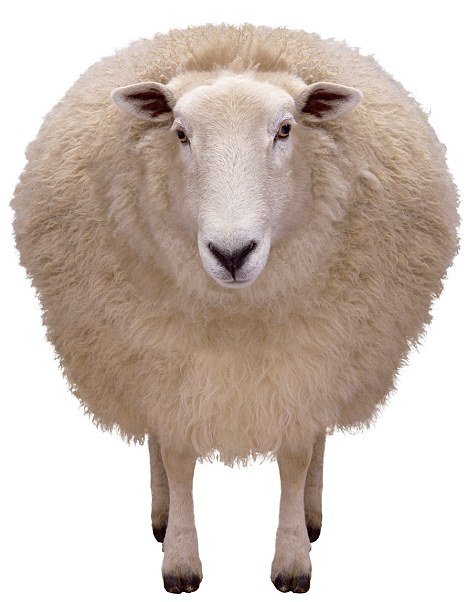
\includegraphics[width=2cm]{figures/sheep.jpg}}

\begin{pollframe}

Let $A = \mat{1 1; 0 1}$ and let $T(x) = Ax$, so $T\colon\R^2\to\R^2$.
($T$ is called a \textbf{shear}.)

\medskip
\begin{bluebox}[Poll]{.8\textwidth}
  What does $T$ do to this sheep?\\[1mm]
  \alert{Hint:} first draw a picture what it does to
  the box \emph{around} the sheep.
\end{bluebox}


\vfill
\hbox to \linewidth{\hss
\begin{tikzpicture}[axes/.pic={
    \draw[->,opacity=.5] (-.8,0) -- (.8,0);
    \draw[->,opacity=.5] (0,-.8) -- (0,.8);
  }]

  \node (sheep1) {\sheep} pic {axes};

 \path (4,0) node[rotate=90] (sheep2) {\sheep} pic {axes};
 \path (7,0) node[cm={1,0,1,1,(0,0)}] (sheep3) {\sheep} pic {axes};
 \path (9.8,0) node (sheep4) {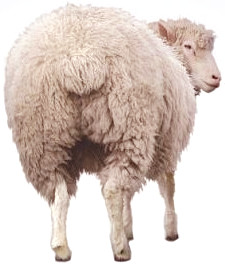
\includegraphics[width=2cm]{figures/sheep_back.jpg}} pic {axes};

  \draw[->,very thick,yshift=1cm] (sheep1.20)
    to[out=20, in=160, "$T$"] (sheep2.north |- sheep1.20);

  \path (4,1.4) node[seq-blue] {$A$}
      ++(3,0) node[seq-blue] {$B$}
      ++(2.8,0) node[seq-blue] {$C$};

  \useasboundingbox (0,-2.1);

  \draw<2->[dashed,seq-blue] (5.4,-1.4) rectangle (8.7,1.7);
  \node<2->[seq-blue] (SS) at (5,-2) {sheared sheep};
  \draw<2->[seq-blue,->,shorten=2pt] (SS.east) to[out=0,in=-90] (7,-1.4);

\end{tikzpicture}
\hss}
\vfill

\end{pollframe}


%%%%%%%%%%%%%%%%%%%%%%%%%%%%%%%%%%%%%%%%%%%%%%%%%%%%%%%%%%%%%%%%%%%

\begin{frame}
\frametitle{Linear Transformations}

\displayskips{3pt}
\alert{Recall:} If $A$ is a matrix, $u,v$ are vectors, and $c$ is a scalar, then
\[ A(u+v) = Au + Av \qquad A(cv) = cAv. \]
\pause
So if $T(x) = Ax$ is a matrix transformation then,
\textcolor<4->{blue}{
\[ T(u+v) = T(u) + T(v)  \qquad  T(cv) = cT(v). \]}%
\pause
This property is so special that it has its own name.

\pause\smallskip
\begin{defn}
  A transformation $T\colon\R^n\to\R^m$ is \textbf{linear} if it satisfies the
  above \textcolor{blue}{equations} for all vectors $u,v$ in $\R^n$ and all
  scalars $c$.
\end{defn}

\pause
In other words, $T$ ``respects'' addition and scalar multiplication.

\pause\bigskip
\alert{Check:} if $T$ is linear, then
\[ T(0) = 0 \qquad T(cu + dv) = cT(u) + dT(v) \]
for all vectors $u,v$ and scalars $c,d$.
\pause
More generally,
\[ T\bigl( c_1v_1 + c_2v_2 + \cdots + c_nv_n \bigr)
 = c_1 T(v_1) + c_2 T(v_2) + \cdots + c_n T(v_n). \]
\pause
In engineering this is called \textbf{superposition}.

\end{frame}


%%%%%%%%%%%%%%%%%%%%%%%%%%%%%%%%%%%%%%%%%%%%%%%%%%%%%%%%%%%%%%%%%%%

\begin{frame}
\frametitle{Linear Transformations}
\framesubtitle{Dilation}

Define $T\colon\R^2\to\R^2$ by $T(x) = 1.5x$.  Is $T$ linear?  Check:
\pause
\[\begin{split} 
  T(u+v) &= \webonlycmd{1.5(u+v) = 1.5u + 1.5v = T(u) + T(v)} \\
  T(cv) &= \webonlycmd{1.5(cv) = c(1.5v) = c(Tv).} \end{split} \]
\pause
So $T$ satisfies the two equations, hence $T$ is linear.

\pause\medskip
This is called \textbf{dilation} or \textbf{scaling} (by a factor of $1.5$).
Picture:

\pause

\def\theo{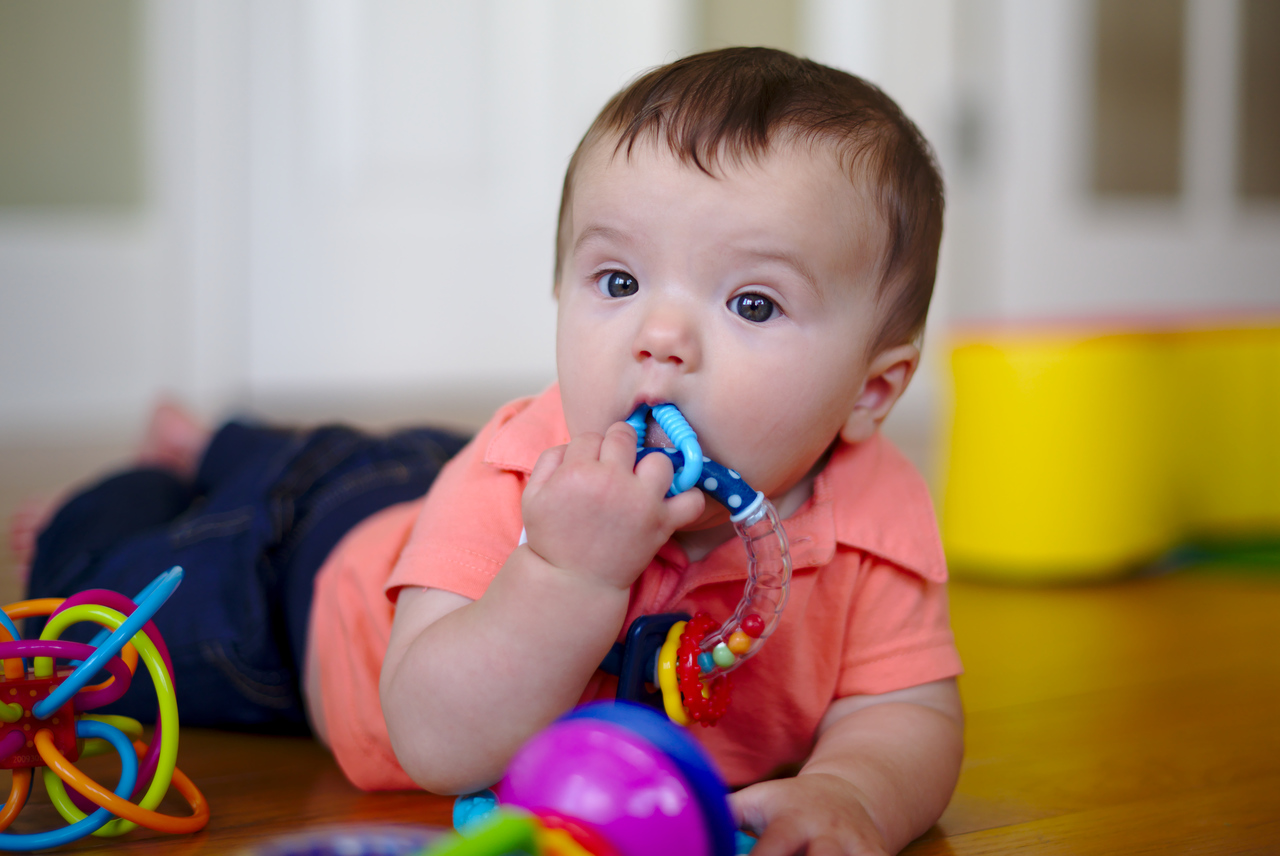
\includegraphics[width=3.5cm]{figures/theo3.jpg}}

\vfill
\hbox to \linewidth{\hss
\begin{tikzpicture}
  \node (theo1) at (0,0,0) {\theo};
  \draw[->,opacity=.6] (-1.3,0) -- (1.3,0);
  \draw[->,opacity=.6] (0,-1.3) -- (0,1.3);

  \begin{scope}[xshift=7cm]
  \node[scale=1.5] (theo2) at (0,0,0) {\theo};
  \draw[->,opacity=.6] (-1.3,0) -- (1.3,0);
  \draw[->,opacity=.6] (0,-1.3) -- (0,1.3);
  \end{scope}

  \draw[->] ($(theo1.east)+(0,.3)$)
    to[bend left, "$T$"] ($(theo2.west)+(0,.3)$);
\end{tikzpicture}
\hss}
\vfill

\end{frame}


%%%%%%%%%%%%%%%%%%%%%%%%%%%%%%%%%%%%%%%%%%%%%%%%%%%%%%%%%%%%%%%%%%%

\def\arcarrow#1;{
  \pgfmathanglebetweenpoints{\pgfpoint{0cm}{0cm}}{\pgfpointanchor{#1}{center}}
  \let\sangle=\pgfmathresult
  \draw[|->, shorten=1mm] 
    let \p1 = (#1.center), \n1={veclen(\x1,\y1)} in
      (#1) arc[radius=\n1, delta angle=90, start angle=\sangle];
}

\begin{frame}
\frametitle{Linear Transformations}
\framesubtitle{Rotation}

Define $T\colon\R^2\to\R^2$ by
\[ T\vec{x y} = \vec{-y x}. \]
Is $T$ linear?  Check:
\pause
\[\begin{split} 
  T\left(\vec{u_1 u_2} + \vec{v_1 v_2}\right)
    &= \webonlycmd{\vec{-u_2 u_1} + \vec{-v_2 v_1}
         = \vec{-(u_2+v_2) (u_1+v_1)} = T\vec{u_1+u_2 v_1+v_2}} \\
  T\left(c\vec{v_1 v_2}\right)
  &= \webonlycmd{T\vec{cv_1 cv_2} = \vec{-cv_2 cv_1}
  = c\vec{-v_2 v_1} = cT\vec{v_1 v_2}.} \end{split} \]

\smallskip
  \begin{minipage}[t]{.6\linewidth}
    \pause
    So $T$ satisfies the two equations, hence $T$ is linear.
    \pause
    This is called \textbf{rotation} (by $90^\circ$).  Picture:
    \[\begin{split}
      \uncover<5->{T\color{seq1}\vec{1 2} &= \color{seq1}\vec{-2 1}} \\
      \uncover<6->{T\color{seq2}\vec{-1 1} &= \color{seq2}\vec{-1 -1}} \\
      \uncover<7->{T\color{seq3}\vec{0 -2} &= \color{seq3}\vec{2 0}} \\
    \end{split}\]
  \end{minipage}
\hfill
\begin{tikzpicture}[scale=.6,baseline=(current bounding box.north)]
  \draw[help lines] (-3,-3) grid (3,3);
  \draw[->] (-3,0) -- (3,0);
  \draw[->] (0,-3) -- (0,3);

  \begin{uncoverenv}<5->
  \point[seq1] (X1) at (1,2);
  \point[seq1] (TX1) at (-2,1);
  \arcarrow X1;
  \end{uncoverenv}

  \begin{uncoverenv}<6->
  \point[seq2] (X2) at (-1,1);
  \point[seq2] (TX2) at (-1,-1);
  \arcarrow X2;
  \end{uncoverenv}

  \begin{uncoverenv}<7->
  \point[seq3] (TX3) at (2,0);
  \point[seq3] (X3) at (0,-2);
  \arcarrow X3;
  \end{uncoverenv}
\end{tikzpicture}

\end{frame}


%%% Local Variables:
%%% TeX-master: "../slides"
%%% End:

% 
\usetikzlibrary{math}

\titleframe{Section 1.9}{The Matrix of a Linear Transformation}


%%%%%%%%%%%%%%%%%%%%%%%%%%%%%%%%%%%%%%%%%%%%%%%%%%%%%%%%%%%%%%%%%%%
% JDR: Students will be asking you until the day of the final what do e_1, e_2,
%   etc. mean...

\begin{frame}
\frametitle{Unit Coordinate Vectors}

\vskip-.3cm

\begin{defn}
  The \textbf{unit coordinate vectors} in $\R^n$ are
  \[ \namedbox{ei}{
    e_1 = \vec{1 0 \vdots, 0 0},\quad e_2 = \vec{0 1 \vdots, 0 0},\quad\ldots,\quad
    e_{n-1} = \vec{0 0 \vdots, 1 0},\quad e_n = \vec{0 0 \vdots, 0 1}.} \]
  \pause
  \begin{tikzpicture}[remember picture, overlay]
    \node[orangebox, fit=(ei)] (ei') {};
    \path (ei'.north) ++(10mm,2.5mm)
      node[anchor=south west, orange, align=left] (expl)
        {This is what $e_1,e_2,\ldots$ mean,\\
          \emph{for the rest of the class}.};
    \draw[->, orange] (expl.west) to[out=180, in=90] ($(ei'.north)+(5mm,0)$);
      
  \end{tikzpicture}
\end{defn}

\pause\hfill
\begin{tikzpicture}[scale=.5, thin border nodes]
  \draw[grid lines] (-2,-2) grid (2,2);
  \draw[->] (-2,0) -- (2,0);
  \draw[->] (0,-2) -- (0,2);
  \draw[vector, seq1] (0,0) to["$e_1$" below=1pt] (1,0);
  \draw[vector, seq2] (0,0) to["$e_2$"] (0,1);
  \node[font=\normalsize, above] at (0,2.1) {in $\R^2$};
  \point at (0,0);
\end{tikzpicture}
\hfill\pause
\begin{tikzpicture}[scale=.5, myxyz, thin border nodes]
  \node[font=\normalsize, above] at (0,0,2.1) {in $\R^3$};
  \useasboundingbox[resetxy] (-2,-2) rectangle (2,2);
  \draw[grid lines, transformxy] (-2,-2) grid (2,2);
  \draw[->] (-2,0,0) -- (2,0,0);
  \draw[->] (0,-2,0) -- (0,2,0);
  \draw[->] (0,0,-2) -- (0,0,2);
  \draw[vector, seq1] (0,0,0) to["$e_1$" below=1pt] (1,0,0);
  \draw[vector, seq2] (0,0,0) to["$e_2$" pos=.8] (0,1,0);
  \draw[vector, seq3] (0,0,0) to["$e_3$"] (0,0,1);
  \point at (0,0,0);
\end{tikzpicture}
\hfill\null

\pause\medskip
\alert{Note:}
if $A$ is an $m\times n$ matrix with columns $v_1,v_2,\ldots,v_n$, then
\textcolor{seq-red}{$Ae_i = v_i$} for $i=1,2,\ldots,n$:
\pause
multiplying a matrix by $e_i$ gives you the $i$th column.

\webonlycmd{\def\A{\mat{1 2 3; 4 5 6; 7 8 9}}\small
\smallskip
\hbox to \linewidth{\hss
$ 
\A\vec{1 0 0} = \vec{1 4 7} \qquad
\A\vec{0 1 0} = \vec{2 5 8} \qquad
\A\vec{0 0 1} = \vec{3 6 9}
$
\hss}
}

\end{frame}


%%%%%%%%%%%%%%%%%%%%%%%%%%%%%%%%%%%%%%%%%%%%%%%%%%%%%%%%%%%%%%%%%%%

\begin{frame}
\frametitle{Linear Transformations are Matrix Transformations}

\alert{Recall:} A matrix $A$ defines a linear transformation $T$ by $T(x) = Ax$.

\pause
\begin{thm}
  Let $T\colon\R^n\to\R^m$ be a linear transformation.  Let
  \[ A = \mat{| | ,, |; T(e_1) T(e_2) \cdots, T(e_n); | | ,, | }. \]
  This is an $\blankuntil{3}{m\times n}$ matrix, 
  \pause 
  and $T$ is the matrix transformation for $A$: $T(x) = Ax$.

  \pause\smallskip
  The matrix $A$ is called the \textbf{standard matrix} for $T$.
\end{thm}

\pause
\begin{bluebox}[Take-Away]{.85\linewidth}\centering
  Linear transformations are the same as matrix transformations.
\end{bluebox}
\note[item]{These are essentially the only transformations we'll deal with in
  this class.}
\note[item]{The added abstraction of linear transformations is useful: sometimes
  a transformation isn't given a priori as a matrix transformation, like in the
  1.8 slides.}

\pause
\hbox to \linewidth{\hfil\alert{Dictionary}\hfil}
\pause\leavevmode
\parbox{.3\linewidth}{\centering
  Linear transformation\\$T\colon\R^n\to\R^m$}%
\;\longsquiggly\;
\hbox to .5\linewidth{$m\times n$ matrix
\small$A = \mat{| | ,, |; T(e_1) T(e_2) \cdots, T(e_n); | | ,, | }$\hss}\\[1mm]
\pause\leavevmode
\hbox to .3\linewidth{\hfil
  $\begin{aligned}&T(x) = Ax\\&T\colon\R^n\to\R^m\end{aligned}$\hfil}%
\;\rlongsquiggly\;
\hbox to .5\linewidth{$m\times n$ matrix $A$\hfil}

\end{frame}


%%%%%%%%%%%%%%%%%%%%%%%%%%%%%%%%%%%%%%%%%%%%%%%%%%%%%%%%%%%%%%%%%%%

\begin{frame}
\frametitle{Linear Transformations are Matrix Transformations}
\framesubtitle{Continued}

\alert{Why is a linear transformation a matrix transformation?}  

\pause\medskip
Suppose for simplicity that $T\colon\R^3\to\R^2$.
\begin{webonly}
\[\begin{split}
  T\vec{x y z} &= T\left( x\vec{1 0 0} + y\vec{0 1 0} + z\vec{0 0 1} \right) \\
  &= T\bigl( xe_1 + ye_2 + ze_3 \bigr) \\
  &= xT(e_1) + yT(e_2) + zT(e_3) \\
  &= \mat{| | |; T(e_1) T(e_2) T(e_3); | | |}\vec{x y z}\\
  &= A\vec{x y z}.
\end{split} \]
\end{webonly}

\end{frame}


%%%%%%%%%%%%%%%%%%%%%%%%%%%%%%%%%%%%%%%%%%%%%%%%%%%%%%%%%%%%%%%%%%%

\begin{frame}
\frametitle{Linear Transformations are Matrix Transformations}
\framesubtitle{Example}

Before, we defined a \textbf{dilation} transformation $T\colon\R^2\to\R^2$ by
$T(x) = 1.5x$.  What is its standard matrix?
\begin{webonly}
\[\left.\begin{aligned}
    T(e_1) &= 1.5e_1 = \vec{1.5 0} \\
    T(e_2) &= 1.5e_2 = \vec{0 1.5}
\end{aligned}\right\}
\implies A = \mat{1.5 0; 0 1.5}.\]
\end{webonly}

\pause
\alert{Check:}
\[ \mat{1.5 0; 0 1.5}\vec{x y} = \pause \vec{1.5x 1.5y}
= \pause 1.5\vec{x y} = T\vec{x y}. \]

\end{frame}


%%%%%%%%%%%%%%%%%%%%%%%%%%%%%%%%%%%%%%%%%%%%%%%%%%%%%%%%%%%%%%%%%%%

\begin{frame}
\frametitle{Linear Transformations are Matrix Transformations}
\framesubtitle{Example}

\vskip -3mm
\begin{ques}
  What is the matrix for the linear transformation
  $T\colon\R^2\to\R^2$ defined by
  \[ T(x) = x \text{ rotated counterclockwise by an angle } \theta? \]
  \pause
  (Check linearity\ldots)
\end{ques}

\begin{webonly}
\begin{center}
\begin{tikzpicture}[scale=2, thin border nodes]
  \clip (-.5,-.2) rectangle (3.5,1.3);

  \draw[help lines] (0,0) circle[radius=1];
  \draw[->] (-1.3,0) -- (1.3,0);
  \draw[->] (0,-1.3) -- (0,1.3);

  \tikzmath{
    coordinate \c;
    \x = cos(37);
    \y = sin(37);
    \c = (\x,\y);
  }

  \coordinate (Te) at (\c);
  \coordinate (cos) at (\cx,0);
  \point (o) at (0,0);
  \pic[draw] {right angle=(o)--(cos)--(Te)};
  \draw[thick vector] (0,0) -- (1,0) 
    node[pos=.9, below=1mm] {$e_1$};
  \draw[thick vector] (0,0) -- (Te)
    node[pos=.7, above left] {$T(e_1)$};
  \draw (.3,0) arc[start angle=0, delta angle=37, radius=.3cm]
    node[midway, right=.2mm, yshift=.5mm] {$\theta$};
  \draw[seq1,thick] (Te) -- (\cx,0) node[midway,right] {$\sin(\theta)$};
  \draw[seq2,thick] (0,0) -- (\cx,0) node[midway,below=1mm] {$\cos(\theta)$};

  \begin{scope}[xshift=3cm]
    \draw[help lines] (0,0) circle[radius=1];
    \draw[->] (-1.3,0) -- (1.3,0);
    \draw[->] (0,-1.3) -- (0,1.3);
  
    \tikzmath{
      coordinate \c;
      \x = -sin(37);
      \y = cos(37);
      \c = (\x,\y);
    }
  
    \coordinate (Te) at (\c);
    \coordinate (sin) at (\cx, 0);
    \point (o) at (0,0);
    \pic[draw] {right angle=(o)--(sin)--(Te)};
    \draw[thick vector] (0,0) -- (0,1) 
      node[pos=.6, right] {$e_2$};
    \draw[thick vector] (0,0) -- (Te)
      node[pos=1.15, inner sep=1pt] {$T(e_2)$};
    \draw (0,.3) arc[start angle=90, delta angle=37, radius=.3cm]
      node[midway, above=.21mm] {$\theta$};
    \draw[seq2,thick] (Te) -- (\cx,0) node[midway,left] {$\cos(\theta)$};
    \draw[seq1,thick] (0,0) -- (\cx,0) node[midway,below=1mm] {$\sin(\theta)$};
      
  \end{scope}

\end{tikzpicture}
\end{center}

\hbox to \linewidth{\hss
$\left.\begin{aligned}
    T(e_1) &= \vec{\color{seq2}\cos(\theta) \color{seq1}\sin(\theta)} \\
    T(e_2) &= \vec{-\color{seq1}\sin(\theta) \color{seq2}\cos(\theta)}
\end{aligned}\right\}
\implies A = 
\mat{\color{seq2}\cos(\theta) -\color{seq1}\sin(\theta);
     \color{seq1}\sin(\theta) \color{seq2}\cos(\theta)}
\quad
\mat{\theta=90^\circ\implies; A=\mat{0 -1; 1 0}; \text{(from before)}}
$\hss}
\end{webonly}

\end{frame}


%%%%%%%%%%%%%%%%%%%%%%%%%%%%%%%%%%%%%%%%%%%%%%%%%%%%%%%%%%%%%%%%%%%

\def\drawarrow#1{
\begin{tikzpicture}[myxyz, scale=0.6, thin border nodes, baseline]
  \path[clip, resetxy] (-2,-2) rectangle (2,2);

  \begin{scope}[transformxy]
    \fill[blue, opacity=.05] (-1.5,-1.5) rectangle (1.5,1.5);
    \draw[step=1cm, help lines, blue!40!black]
      (-1.5, -1.5) grid (1.5, 1.5);
  \end{scope}

  \node[blue!40!black] at (-.9,1,-.5) {$xy$};

  \begin{scope}[transformyz]
    \fill[green, opacity=.05] (-1.5,-1.5) rectangle (1.5,1.5);
    \draw[step=1cm, help lines, green!40!black]
      (-1.5, -1.5) grid (1.5, 1.5);
  \end{scope}

  \node[green!40!black] at (.75,-1,1) {$yz$};

  #1

\end{tikzpicture}
}

\begin{frame}
\frametitle{Linear Transformations are Matrix Transformations}
\framesubtitle{Example}

\vskip-3mm
\begin{ques}
  What is the matrix for the linear transformation $T\colon\R^3\to\R^3$ that
  reflects through the $xy$-plane and then projects onto the $yz$-plane?
\end{ques}

\pause\vfill

\hbox to \linewidth{\hss
\drawarrow{\draw[vector] (0,0,0) -- (1,0,0) node[above] {$e_1$};}
\longsquiggly[reflect $xy$]
\pause
\drawarrow{\draw[vector] (0,0,0) -- (1,0,0);}
\longsquiggly[project $yz$]
\pause
\drawarrow{\point at (0,0,0);}
\hss}

\pause\medskip

\[ T(e_1) = \vec{0 0 0}. \]

\vfill

\end{frame}

\begin{frame}
\frametitle{Linear Transformations are Matrix Transformations}
\framesubtitle{Example, continued}

\vskip-3mm
\begin{ques}
  What is the matrix for the linear transformation $T\colon\R^3\to\R^3$ that
  reflects through the $xy$-plane and then projects onto the $yz$-plane?
\end{ques}

\vfill

\hbox to \linewidth{\hss
\drawarrow{\draw[vector] (0,0,0) -- (0,1,0) node[below right=-.5mm] {$e_2$};}
\longsquiggly[reflect $xy$]
\pause
\drawarrow{\draw[vector] (0,0,0) -- (0,1,0);}
\longsquiggly[project $yz$]
\pause
\drawarrow{\draw[vector] (0,0,0) -- (0,1,0);}
\hss}

\pause\medskip
\[ T(e_2) = e_2 = \vec{0 1 0}. \]

\vfill

\end{frame}


\begin{frame}
\frametitle{Linear Transformations are Matrix Transformations}
\framesubtitle{Example, continued}

\vskip-3mm
\begin{ques}
  What is the matrix for the linear transformation $T\colon\R^3\to\R^3$ that
  reflects through the $xy$-plane and then projects onto the $yz$-plane?
\end{ques}

\vfill

\hbox to \linewidth{\hss
\drawarrow{\draw[vector] (0,0,0) -- (0,0,1) node[right] {$e_3$};}
\longsquiggly[reflect $xy$]
\pause
\drawarrow{\draw[vector] (0,0,0) -- (0,0,-1);}
\longsquiggly[project $yz$]
\pause
\drawarrow{\draw[vector] (0,0,0) -- (0,0,-1);}
\hss}

\pause\medskip
\[ T(e_3) = \vec{0 0 -1}. \]

\vfill

\end{frame}


\begin{frame}
\frametitle{Linear Transformations are Matrix Transformations}
\framesubtitle{Example, continued}

\vskip-3mm
\begin{ques}
  What is the matrix for the linear transformation $T\colon\R^3\to\R^3$ that
  reflects through the $xy$-plane and then projects onto the $yz$-plane?
\end{ques}

\vfill

\[\left.\begin{aligned}
  T(e_1) &= \vec{0 0 0} \\
  T(e_2) &= \vec{0 1 0} \\
  T(e_1) &= \vec{0 0 -1} \\
\end{aligned}\right\}
\implies A = \pause\mat{0 0 0; 0 1 0; 0 0 -1}.
\]

\vfill

\end{frame}


%%%%%%%%%%%%%%%%%%%%%%%%%%%%%%%%%%%%%%%%%%%%%%%%%%%%%%%%%%%%%%%%%%%

\begin{frame}
\frametitle{Other Geometric Transformations}

\vfill

\begin{bluebox}{.75\textwidth}
  There is a long list of geometric transformations of $\R^2$ in \S1.9 of Lay.
  (Reflections over the diagonal, contractions and expansions along different
  axes, shears, projections, \ldots)
  Please look them over.
\end{bluebox}

\vfill

\end{frame}


%%%%%%%%%%%%%%%%%%%%%%%%%%%%%%%%%%%%%%%%%%%%%%%%%%%%%%%%%%%%%%%%%%%

\begin{frame}
\frametitle{Onto Transformations}

\vskip -.3cm
\begin{defn}
  A transformation $T\colon\R^n\to\R^m$ is \textbf{onto} (or
  \textbf{surjective}) if the range of $T$ is equal to $\R^m$ (its codomain).  
  \pause
  In other words, each $b$
  in $\R^m$ is the image of \emph{at least one} $x$ in $\R^n$:
  \pause
  every possible output has an input.
  \pause
  Note that \emph{not} onto means 
  \pause
  there is some $b$ in $\R^m$ which is not the image of any $x$ in $\R^n$.
\end{defn}
\note{Beware quantifiers}

\pause

\begin{center}
\begin{tikzpicture}[scale=.4, thin border nodes]
  \draw (-3,-3) rectangle (3,3);

  \draw[->, very thin, myxyz] (-2,0,0) -- (2,0,0);
  \draw[->, very thin, myxyz] (0,-2,0) -- (0,2,0);
  \draw[->, very thin, myxyz] (0,0,-2) -- (0,0,2);

  \node (source) at (0,-3.6) {$\R^n$};
  \point["$x$" above left] (x) at (1,2);

  \begin{scope}[xshift=12cm, every label/.append style={fill=seq4!10}]
    \fill[seq4!10] (-3,-3) rectangle (3,3);
    \draw[grid lines] (-3,-3) grid (3,3);
    \point["$T(x)$" above right] (Tx) at (1,-1);
    \node[fill=seq4!10, text=seq4]
      at (0,2) {$\range(T)$};

    \node (target) at (0,-3.6) {$\R^m =$ codomain};
  \end{scope}

  \draw[->] (source) -- (target) node[midway,above=1pt] {$T$};
  \draw[|->, shorten=.35mm] (x) to[out=0, in=180] (Tx);

  \node[seq-blue] at (6,2.5) {onto};

\end{tikzpicture}

\bigskip\pause

\begin{tikzpicture}[scale=.4, thin border nodes]
  \draw (-3,-3) rectangle (3,3);

  \draw[->, very thin, myxyz] (-2,0,0) -- (2,0,0);
  \draw[->, very thin, myxyz] (0,-2,0) -- (0,2,0);
  \draw[->, very thin, myxyz] (0,0,-2) -- (0,0,2);

  \node (source) at (0,-3.6) {$\R^n$};
  \point["$x$" above left] (x) at (1,-2);

  \begin{scope}[xshift=12cm]
    \draw[grid lines] (-3,-3) grid (3,3);
    \draw[seq4] (-3,-1.5) -- (3,1.5); 
   \point["$T(x)$" below right] (Tx) at (1,.5);
    \node[fill=white, text=seq4]
      at (-1,-1.8) {$\range(T)$};

    \node (target) at (0,-3.6) {$\R^m =$ codomain};
  \end{scope}

  \draw[->] (source) -- (target) node[midway,above=1pt] {$T$};
  \draw[|->, shorten=.35mm] (x) to[out=0, in=150] (Tx);

  \node[seq-blue] at (6,2.5) {not onto};

\end{tikzpicture}
\end{center}

\end{frame}


%%%%%%%%%%%%%%%%%%%%%%%%%%%%%%%%%%%%%%%%%%%%%%%%%%%%%%%%%%%%%%%%%%%

\begin{frame}
\frametitle{Characterization of Onto Transformations}

\vskip -3mm
\begin{thm}
  Let $T\colon\R^n\to\R^m$ be a linear transformation with matrix $A$.  Then the
  following are equivalent:
  \begin{itemize}
  \item $T$ is onto
    \pause
  \item $T(x) = b$ has a solution for every $b$ in $\R^m$
    \pause
  \item $Ax = b$ is consistent for every $b$ in $\R^m$
    \pause
  \item The columns of $A$ span $\R^m$
    \pause
  \item $A$ has a pivot in every \blankuntil{6}{row}
  \end{itemize}
\end{thm}

\pause[7]

\begin{ques}
  If $T\colon\R^n\to\R^m$ is onto, what can we say about the relative sizes of
  $n$ and $m$?
\end{ques}

\pause
\alert{Answer:} $T$ corresponds to an \blankuntil{9}{$m\times n$} matrix $A$.
\pause[10]
In order for $A$ to have a pivot in every row, it must have
\emph{at least as many} columns as rows: $m\leq n$.
\pause
\[ \mat{
\color{red}1   0   \star,   0   \star ;
0   \color{red}1   \star , 0   \star ;
0   0   0   \color{red}1   \star 
} \]
\pause
For instance, $\R^2$ is ``too small'' to map \emph{onto\/} $\R^3$.

\end{frame}


%%%%%%%%%%%%%%%%%%%%%%%%%%%%%%%%%%%%%%%%%%%%%%%%%%%%%%%%%%%%%%%%%%%

\begin{frame}
\frametitle{One-to-one Transformations}

\vskip -3mm
\begin{defn}
  A transformation $T\colon\R^n\to\R^m$ is \textbf{one-to-one} (or
  \textbf{into}, or \textbf{injective}) if different vectors in $\R^n$ map to
  different vectors in $\R^m$.
  \pause
  In other words, each $b$ in $\R^m$ is the image of
  \emph{at most one} $x$ in $\R^n$:
  \pause
  different inputs have different outputs.
  \pause
  Note that \emph{not} one-to-one means
  \pause
  different vectors in $\R^n$ have the same image.
\end{defn}

\pause

\begin{center}
\begin{tikzpicture}[scale=0.4, thin border nodes]
  \draw[grid lines] (-3,-3) grid (3,3);

  \node (A) at (0,-3.6) {$\R^n$};
  \node (B) at (12,-3.6) {$\R^m$};
  \draw[->] (A) -- (B) node[midway,above=1pt] {$T$};

  \point["$x$" left] (x) at (1,1.5);
  \point["$y$" left] (y) at (-1,0);
  \point["$z$" left] (z) at (0,-2);

  \begin{scope}[myxyz, xshift=12cm]
    \path[clip, resetxy] (-3,-3) rectangle (3,3);

    \def\v{(2,-1,1)}
    \def\w{(1,0,-1)}
  
    \node[coordinate] (X) at \v {};
    \node[coordinate] (Y) at \w {};

    \draw[very thin] (-2,0,0) -- (0,0,0);
    \draw[very thin] (0,-2,0) -- (0,0,0);
    \draw[very thin] (0,0,-2) -- (0,0,0);

    \begin{scope}[x=(X), y=(Y), transformxy,
        every label/.style={font=\tiny,fill=none,inner sep=.5pt}]
      \fill[seq4!10, nearly opaque] (-1,-1) rectangle (1,1);
      \draw[step=.5cm, seq4!30, very thin] (-1,-1) grid (1,1);
      \point["$T(x)$" above] (Tx) at (.5,-.5);
      \point["$T(y)$" above] (Ty) at (.5,.5);
      \point["$T(z)$" above] (Tz) at (-.5,.75);
      \node[coordinate,
          pin={[pin edge={very thin,-},
            pin distance=3mm,anchor=north,text=seq4]-70:range}]
        at (0.1,1) {};
    \end{scope}

    \draw[->, very thin] (0,0,0) -- (2,0,0);
    \draw[->, very thin] (0,0,0) -- (0,2,0);
    \draw[->, very thin] (0,0,0) -- (0,0,2);

    \draw[resetxy] (-3,-3) rectangle (3,3);

  \end{scope}

  \begin{scope}[arrows={|->}, shorten=.35mm, every to/.style={out=0, in=180}]
    \draw (x) to (Tx);
    \draw (y) to (Ty);
    \draw (z) to (Tz);
  \end{scope}

  \node[seq-blue] at (6,2.5) {one-to-one};

\end{tikzpicture}

\bigskip\pause

\begin{tikzpicture}[scale=0.4, thin border nodes]
  \draw[grid lines] (-3,-3) grid (3,3);

  \node (A) at (0,-3.6) {$\R^n$};
  \node (B) at (12,-3.6) {$\R^m$};
  \draw[->] (A) -- (B) node[midway,above=1pt] {$T$};

  \point["$x$" left] (x) at (1,1.5);
  \point["$y$" left] (y) at (-1,0);
  \point["$z$" left] (z) at (0,-2);

  \begin{scope}[myxyz, xshift=12cm,
      every label/.style={font=\tiny, fill=none, inner sep=.5pt}]
    \path[clip, resetxy] (-3,-3) rectangle (3,3);

    \def\v{(1,-1,2)}
    \node[coordinate] (V) at \v {};
  
    \draw[very thin] (-2,0,0) -- (0,0,0);
    \draw[very thin] (0,-2,0) -- (0,0,0);
    \draw[very thin] (0,0,-2) -- (0,0,0);

    \draw[seq4] ($-4*(V)$) -- ($4*(V)$);
    \point[label={[xshift=.25cm,fill=white]above:{$T(x)=T(y)$}}]
      (Tx) at ($.5*(V)$);
    \point["$T(z)$" right] (Tz) at ($-1*(V)$);
    \node[coordinate,
        pin={[pin edge={very thin,-},
          pin distance=8mm,anchor=north,text=seq4]-30:range}]
        at ($-.2*(V)$) {};

    \draw[->, very thin] (0,0,0) -- (2,0,0);
    \draw[->, very thin] (0,0,0) -- (0,2,0);
    \draw[->, very thin] (0,0,0) -- (0,0,2);

    \draw[resetxy] (-3,-3) rectangle (3,3);

  \end{scope}

  \begin{scope}[arrows={|->}, shorten=.35mm, every to/.style={out=0, in=180}]
    \draw (x) to (Tx);
    \draw[|-] (y) to (Tx);
    \draw (z) to (Tz);
  \end{scope}

  \node[seq-blue] at (6,2.5) {not one-to-one};

\end{tikzpicture}

\end{center}

\end{frame}


%%%%%%%%%%%%%%%%%%%%%%%%%%%%%%%%%%%%%%%%%%%%%%%%%%%%%%%%%%%%%%%%%%%

\begin{frame}
\frametitle{Characterization of One-to-One Transformations}

\vskip -3mm
\begin{thm}
  Let $T\colon\R^n\to\R^m$ be a linear transformation with matrix $A$.  Then the
  following are equivalent:
  \begin{itemize}
  \item $T$ is one-to-one
    \pause
  \item $T(x) = b$ has one or zero solutions for every $b$ in $\R^m$
    \pause
  \item $Ax = b$ has a unique solution or is inconsistent for every $b$ in $\R^m$
    \pause
  \item $Ax = 0$ has a unique solution
    \pause
  \item The columns of $A$ are linearly independent
    \pause
  \item $A$ has a pivot in every \blankuntil{7}{column}.
  \end{itemize}
\end{thm}

\pause[8]

\begin{ques}
  If $T\colon\R^n\to\R^m$ is one-to-one, what can we say about the relative sizes of
  $n$ and $m$?
\end{ques}

\pause
\alert{Answer:} $T$ corresponds to an $m\times n$ matrix $A$.
\pause
In order for $A$ to have a pivot in every column, it must have
\emph{at least as many} rows as columns: $n\leq m$.

\pause
\hbox to \linewidth{\hss
\begin{minipage}{.4\textwidth}
\[ \mat{
\color{red}1   0   0 ;
0   \color{red}1  0 ;
0 0  \color{red}1 ;
0 0 0
} \]
\end{minipage}
\pause
\begin{minipage}{.6\textwidth}
For instance, $\R^3$ is ``too big'' to map \emph{into\/} $\R^2$.
\end{minipage}\hss}

\end{frame}


%%% Local Variables:
%%% TeX-master: "../slides"
%%% End:

% 
% JDR: These are the topics I thought my students found most confusing from
%   chapter 1, and the ones they asked me to cover.  They can probably be covered
%   in 50 minutes, but aren't necessarily meant to--the students can always review
%   the rest online.

\titleframe{Review for Midterm 1}{Selected Topics}


%%%%%%%%%%%%%%%%%%%%%%%%%%%%%%%%%%%%%%%%%%%%%%%%%%%%%%%%%%%%%%%%%%%

\begin{frame}
\frametitle{Linear Equations}

We have \emph{four} equivalent ways of writing (and thinking about) linear
systems:
\pause
\begin{enumerate}
\item As a system of equations:
\[ \syseq{2x_1 + 3x_2 = 7; x_1 - x_2 = 5} \]
\vskip-5mm\pause
\item As an augmented matrix:
  \vskip -3mm
  \[ \amat{ 2 3 7; 1 -1 5} \]
\vskip-5mm\pause
\item As a vector equation ($x_1v_1 + \cdots + x_nv_n = b$):
  \[ x_1\vec{2 1} + x_2\vec{3 -1} = \vec{7 5} \]
\vskip-7mm\pause
\item As a matrix equation ($Ax = b$):
  \[ \mat{ 2 3; 1 -1}\vec{x_1 x_2} = \vec{7 5} \]
  \note{(4) is by definition equal to (3).}%
\end{enumerate}
\pause

In particular, \emph{all four have the same solution set}.

\end{frame}


%%%%%%%%%%%%%%%%%%%%%%%%%%%%%%%%%%%%%%%%%%%%%%%%%%%%%%%%%%%%%%%%%%%

\begin{frame}
\frametitle{Number of Solutions}

There are \emph{three possibilities} for the reduced row echelon form of the
augmented matrix of a linear system.\pause

\begin{enumerate}
\item \alert{The last column is a pivot column.}\\
  \pause
  There are \emph{zero} solutions, i.e.\ the solution set is \emph{empty}.
  \pause
  In this case, the system is called \textbf{inconsistent}.  
  Picture:
  \pause
  \[ \amat{ 1 0 {\color{red}0}; 0 1 {\color{red}0}; 0 0 {\color{red}1}} \]

\pause
\item \alert{Every column except the last column is a pivot column.}\\
  In this case, the system has a \emph{unique solution}.  Picture:
  \[ \amat{
      1  0  0  \star ;
      0  1  0  \star ;
      0  0  1  \star
    } \]
\note{Ask: what are $x,y,z$?}%

\pause
\item \alert{The last column is not a pivot column, and some other column isn't either.}\\
  In this case, the system has \emph{infinitely many} solutions, corresponding
  to the infinitely many possible values of the free variable(s).  Picture:
  \[\amat{
      1  \color{seq-red}\star,  0  \color{seq-blue}\star,  \star ;
      0  \color{seq-red}0   1  \color{seq-blue}\star, \star
    }\]

\end{enumerate}

\end{frame}


%%%%%%%%%%%%%%%%%%%%%%%%%%%%%%%%%%%%%%%%%%%%%%%%%%%%%%%%%%%%%%%%%%%

\begin{frame}
\frametitle{Span}

The \textbf{span} of vectors $v_1,v_2,\ldots,v_n$ is the set of all linear
combinations of these vectors:
\[ \Span\{v_1,v_2,\ldots,v_n\}
= \bigl\{ a_1v_1+a_2v_2+\cdots+a_nv_n\mid a_1,a_2,\ldots,a_n\text{ in }\R \bigr\}. \]

\pause
\begin{thm}
  Let $v_1,v_2,\ldots,v_n$, and $b$ be vectors in $\R^m$, and let $A$ be the
  $m\times n$ matrix with columns $v_1,v_2,\ldots,v_n$.  The following are
  equivalent\namedbox{colon}{:}
  \begin{tikzpicture}[remember picture, overlay, blue!50]
    \path (colon.east) ++(1.2cm,.2cm) node[anchor=north west, text width=3cm]
      (expl) {either they're all true, or they're all false, for the given vectors};
    \draw[->, thick] (expl.west) to[out=180, in=0] (colon.east);
  \end{tikzpicture}
  \begin{enumerate}
    \pause
  \item $Ax = b$ is consistent.
    \pause
  \item $(\,A\mid b\,)$ does not have a pivot in \pause the last column.
    \pause
  \item $b$ is in $\Span\{v_1,v_2,\ldots,v_n\}$ (the span of the columns of
    $A$).
  \end{enumerate}
\end{thm}

\pause
In this case, a solution to the matrix equation
\[ A\vec{x_1 x_2 \vdots, x_n} = b
\parbox{3cm}{\centering gives the linear\\combination}
x_1v_1 + x_2v_2 + \cdots + x_nv_n = b. \]

\end{frame}


%%%%%%%%%%%%%%%%%%%%%%%%%%%%%%%%%%%%%%%%%%%%%%%%%%%%%%%%%%%%%%%%%%%

\begin{frame}
\frametitle{Transformations}

\vskip-3mm
\begin{defn}
  A \textbf{transformation} (or \textbf{function} or \textbf{map}) from $\R^n$
  to $\R^m$ is a rule $T$ that assigns to each vector $x$ in $\R^n$ a vector
  $T(x)$ in $\R^m$.
\end{defn}

\pause
Picture and vocabulary words:

\begin{center}
\begin{tikzpicture}[scale=0.35, baseline, thin border nodes]
  \path[use as bounding box] (-3,-5.5) -- (15,3);
  \draw[grid lines] (-3,-3) grid (3,3);

  \node (A) at (0,-4) {$\R^n$};
  \node (B) at (12,-4) {$\R^m$};
  \node at (0,-5) {domain};
  \node at (12,-5) {codomain};
  \draw[->] (A.east) +(5mm,0) -- node[midway,above=1pt] {$T$}
    ($(B.west)-(5mm,0)$);

  \point["$x$" left] (P) at (1,1.5);

  \begin{scope}[myxyz, xshift=12cm]
    \path[clip, resetxy] (-3,-3) rectangle (3,3);

    \def\v{(2,-1,1)}
    \def\w{(1,0,-1)}
  
    \node[coordinate] (X) at \v {};
    \node[coordinate] (Y) at \w {};

    \draw[very thin] (-2,0,0) -- (0,0,0);
    \draw[very thin] (0,-2,0) -- (0,0,0);
    \draw[very thin] (0,0,-2) -- (0,0,0);

    \begin{scope}[x=(X), y=(Y), transformxy]
      \fill[seq4!10, nearly opaque] (-1,-1) rectangle (1,1);
      \draw[step=.5cm, seq4!30, very thin] (-1,-1) grid (1,1);
      \point[label={[font=\tiny,fill=none]below:$T(x)$}]
        (Q) at (-.5,.5);
      \node[coordinate,
          pin={[pin edge={very thin,-},pin distance=3mm,anchor=north,font=\small,xshift=1mm,text=seq4]-90:range}]
        at (0.1,1) {};
    \end{scope}

    \draw[->, very thin] (0,0,0) -- (2,0,0);
    \draw[->, very thin] (0,0,0) -- (0,2,0);
    \draw[->, very thin] (0,0,0) -- (0,0,2);

    \draw[resetxy] (-3,-3) rectangle (3,3);

  \end{scope}

  \pic[scale=.4, "$T$"] (machine) at (6,0) {machine};
  \draw[->, shorten >=.35mm, shorten <=.35mm] (P.east)
    .. controls +(0:1cm) and +(180:1cm) .. (machine-input);
  \draw[->, shorten >=.35mm, shorten <=.35mm] (machine-output)
    .. controls +(0:1cm) and +(190:2cm) .. (Q.west);

\end{tikzpicture}
\end{center}

\pause
It is \textbf{one-to-one} if different vectors in the domain go to different
vectors in the codomain: $x\neq y\implies T(x)\neq T(y)$.

\pause\medskip
It is \textbf{onto} if every vector in the codomain is $T(x)$ for some $x$.
\pause
In other words, the range equals the codomain.

\end{frame}


%%%%%%%%%%%%%%%%%%%%%%%%%%%%%%%%%%%%%%%%%%%%%%%%%%%%%%%%%%%%%%%%%%%

\begin{frame}
\frametitle{Linear Transformations}

A transformation $T\colon\R^n\to\R^m$ is \textbf{linear} if it satisfies:
\[ T(u+v) = T(u) + T(v) \sptxt{and} T(cu) = cT(u) \]
for every $u,v$ in $\R^n$ and every $c$ in $\R$.

\pause\smallskip
\begin{bluebox}{.85\linewidth}\centering
  Linear transformations are the same as matrix transformations.
\end{bluebox}

\pause
\hbox to \linewidth{\hfil\alert{Dictionary}\hfil}
\pause\leavevmode
\parbox{.3\linewidth}{\centering
  Linear transformation\\$T\colon\R^n\to\R^m$}%
\;\longsquiggly\;
\hbox to .5\linewidth{$m\times n$ matrix
\small$A = \mat{| | ,, |; T(e_1) T(e_2) \cdots, T(e_n); | | ,, | }$\hss}\\[1mm]
\pause\leavevmode
\hbox to .3\linewidth{\hfil
  $\begin{aligned}&T(x) = Ax\\&T\colon\R^n\to\R^m\end{aligned}$\hfil}%
\;\rlongsquiggly\;
\hbox to .5\linewidth{$m\times n$ matrix $A$\hfil}

\pause\smallskip
As always, $e_1,e_2,\ldots,e_n$ are the \textbf{unit coordinate vectors}\small
\[ e_1 = \vec{1 0 \vdots, 0 0},\quad e_2 = \vec{0 1 \vdots, 0 0},\quad\ldots,\quad
   e_{n-1} = \vec{0 0 \vdots, 1 0},\quad e_n = \vec{0 0 \vdots, 0 1}. \]

\end{frame}


%%%%%%%%%%%%%%%%%%%%%%%%%%%%%%%%%%%%%%%%%%%%%%%%%%%%%%%%%%%%%%%%%%%

\begin{frame}
\frametitle{Linear Transformations and Matrices}

Let $A$ be an $m\times n$ matrix and let $T$ be the linear transformation
$T(x)=Ax$.
\begin{itemize}
  \pause
\item The domain of $T$ is $\R^n$.  (Inputs are vectors with $n$ entries.)
  \pause
\item The codomain of $T$ is $\R^m$.  (Outputs are vectors with $m$ entries.)
  \pause
\item The range of $T$ is span of the columns of $A$.\\
  \pause
  (This is the set of all
  $b$ in $\R^m$ such that $Ax=b$ has a solution.)
\end{itemize}

\pause\leavevmode
\begin{minipage}[t]{.5\textwidth}
\begin{eg}
  \vskip -.5cm
  \[ A = \mat[r]{2 1; -1 0; 1 -1} \qquad T(x) = Ax \]
  \begin{itemize}
  \item<7-> The domain of $T$ is $\R^{\blankuntil{8}2}$.
  \item<9-> The codomain of $T$ is $\R^{\blankuntil{10}3}$.
  \item<11-> The range of $T$ is 
    \uncover<12->{\[ \Span\left\{\textcolor{seq-red}{\vec{2 -1 1}},\,
        \textcolor{seq-blue}{\vec{1 0 -1}}\right\}. \]}
  \end{itemize}
\end{eg}
\end{minipage}\quad
\begin{uncoverenv}<12->
\begin{tikzpicture}[myxyz, scale=.6, baseline=3cm]
  \begin{scope}
  \path[clip, resetxy] (-4,-3) rectangle (4,3);

  \def\v{(2,-1,1)}
  \def\w{(1,0,-1)}

  \node[coordinate] (X) at \v {};
  \node[coordinate] (Y) at \w {};

  \begin{scope}[x=(X), y=(Y), transformxy]
    \path[clip] (-5, -5) -- (5, 5) -- (5, 10) -- (-5, 10) -- cycle;
    \fill[seq4!10, nearly opaque] (-1.5,-1) rectangle (1.5,2);
    \draw[step=.5cm, seq4!30, very thin] (-1.5,-1) grid (1.5,2);
  \end{scope}

  \begin{scope}[transformxy]
    \fill[white, semitransparent] (-2, -2) rectangle (3, 3);
    \draw[step=1cm, grid lines] (-2, -2) grid (3, 3);
  \end{scope}

  \begin{scope}[x=(X), y=(Y), transformxy]
    \path[clip] (-5, -5) -- (5, 5) -- (5, -10) -- (-5, -10) -- cycle;
    \fill[seq4!10, nearly opaque] (-1.5,-1) rectangle (1.5,2);
    \draw[step=.5cm, seq4!30, very thin] (-1.5,-1) grid (1.5,2);
  \end{scope}

  \draw[vector, seq1] (0,0,0) -- \v;
  \draw[thin, densely dotted] \v -- \projxy\v;

  \draw[vector, seq2!50!white] (0,0,0) -- \w;
  \draw[thin, densely dotted, black!50!white] \w -- \projxy\w;

  \node[seq4] at (-1.5cm, 1.5cm) {$\range(T)$};

  \point at (0,0,0) {};
  \draw[thin,resetxy] (-4,-3) rectangle (4,3);
  \end{scope}
  \node at (0,-3.5cm) {$\R^3 = {\rm codomain}(T)$};
\end{tikzpicture}
\end{uncoverenv}

\end{frame}


%%%%%%%%%%%%%%%%%%%%%%%%%%%%%%%%%%%%%%%%%%%%%%%%%%%%%%%%%%%%%%%%%%%

\begin{frame}
\frametitle{When the Span is Everything}

\vskip-3mm

\begin{thm}
  Let $A$ be an $m\times n$ matrix, and let $T\colon\R^n\to\R^m$ be the linear
  transformation $T(x) = Ax$.  The following are equivalent:
  \begin{enumerate}
    \pause
  \item $T$ is onto.
    \pause
  \item $T(x) = b$ has a solution for every $b$ in $\R^m$.
    \pause
  \item $Ax = b$ is consistent for every $b$ in $\R^m$.
    \pause
  \item The columns of $A$ span $\R^m$.
    \pause
  \item A has a pivot in each \emph{row}.
  \end{enumerate}
\end{thm}

\pause
\alert{Moral:}
If $A$ has a pivot in each row then its reduced row echelon form looks like this:
\[\def\r{\color{red}} \mat{
\r1   0   \star,   0   \star ;
0   \r1   \star , 0   \star ;
0   0   0   \r1   \star 
}
\pause\quad\parbox{.2\textwidth}
{\centering and $(\,A\mid b\,)$ reduces to this:}\quad
\amat[c]{
\r1   0   \star,   0   \star, \star ;
0   \r1   \star , 0   \star, \star ;
0   0   0   \r1   \star, \star 
}.\]
\pause
There's no $b$ that makes it inconsistent, so there's always a solution.

\pause\medskip
\alert{Refer:} slides for \S1.4 and \S1.9.

\end{frame}


%%%%%%%%%%%%%%%%%%%%%%%%%%%%%%%%%%%%%%%%%%%%%%%%%%%%%%%%%%%%%%%%%%%

\begin{frame}
\frametitle{Linear Independence}

A \emph{set} of vectors $\{v_1,v_2,\ldots,v_n\}$ is
\textbf{linearly independent} if
\[ a_1v_1 + a_2v_2 + \cdots + a_nv_n = 0 
\sptxt{only when} a_1 = a_2 = \cdots = a_n = 0. \]
\pause
Otherwise they are \textbf{linearly dependent}, and an equation
$a_1v_1 + a_2v_2 + \cdots + a_nv_n = 0$
with some $a_i\neq0$ is a \textbf{linear dependence relation}.

\pause
\begin{thm}
  Let $v_1,v_2,\ldots,v_n$ be vectors in $\R^m$, and let $A$ be the
  $m\times n$ matrix with columns $v_1,v_2,\ldots,v_n$.  The following are
  equivalent:
  \begin{enumerate}
    \pause
  \item The set $\{v_1,v_2,\ldots,v_n\}$ is linearly independent.
    \pause
  \item For every $i$ between $1$ and $n$, $v_i$ is not in
    $\Span\{v_1,v_2,\ldots,v_{i-1}\}$.
    \pause
  \item $Ax=0$ only has the trivial solution.
    \pause
  \item $A$ has a pivot in every \blankuntil{8}{column}\pause.
  \end{enumerate}
\end{thm}

\pause
If the vectors are linearly \emph{de}pendent, a nontrivial solution to the
matrix equation
\[ A\vec{x_1 x_2 \vdots, x_n} = 0
\parbox{3.5cm}{\centering gives the linear\\dependence relation}
x_1v_1 + x_2v_2 + \cdots + x_nv_n = 0. \]

\end{frame}


%%%%%%%%%%%%%%%%%%%%%%%%%%%%%%%%%%%%%%%%%%%%%%%%%%%%%%%%%%%%%%%%%%%

\begin{frame}
\frametitle{More Criteria for Linear Independence}

\vskip-3mm

\begin{thm}
  Let $A$ be an $m\times n$ matrix, and let $T\colon\R^n\to\R^m$ be the linear
  transformation $T(x) = Ax$.  The following are equivalent:
  \begin{enumerate}
    \pause
  \item $T$ is one-to-one.
    \pause
  \item $T(x) = b$ has one or zero solutions for every $b$ in $\R^m$.
    \pause
  \item $Ax = b$ has a unique solution or is inconsistent for every $b$ in $\R^m$.
    \pause
  \item $Ax = 0$ has a unique solution.
    \pause
  \item The columns of $A$ are linearly independent.
    \pause
  \item A has a pivot in each \emph{column}.
  \end{enumerate}
\end{thm}

\pause
\alert{Moral:}
If $A$ has a pivot in each column then its reduced row echelon form looks like this:
\[\def\r{\color{red}} \mat{
\r1   0   0 ;
0   \r1   0 ;
0     0   \r1 ;
0     0   0 
}
\pause\quad\parbox{.2\textwidth}
{\centering and $(\,A\mid b\,)$ reduces to this:}\quad
\amat[c]{
\r1   0   0 \star;
0   \r1   0 \star;
0     0   \r1 \star ;
0     0   0 \star
}.\]
\pause
This can be inconsistent, but if it is consistent, it has a unique solution.

\pause\medskip
\alert{Refer:} slides for \S1.4, \S1.8, \S1.9.

\end{frame}


%%%%%%%%%%%%%%%%%%%%%%%%%%%%%%%%%%%%%%%%%%%%%%%%%%%%%%%%%%%%%%%%%%%

\begin{frame}
\frametitle{Parametric Form of Solution Sets}

To find the solution set to $Ax=b$, first form the augmented matrix
$(\,A\mid b\,)$, then row reduce.
\pause
\def\r{\color<5->{red}}\def\g{\color<5->{green!70!black}}
\[ \amat{1 \r3 0  \g4 0 2;
         0 \r0 1 \g{-1} 0 3;
         0 \r0 0  \g0 1 -7} \]
\pause
This translates into
\spalignsysdelims..
\[ \syseq{x_1 + \r3x_2 \+ \.  \+ \g{x_4} \+ \.  = 2;
          \. \+  \.  \+ x_3  - \g{x_4}  \+ \.  = 3;
          \. \+  \.  \+ \.  \+  \.  \+ x_5 = -7} \]
\pause
The variables correspond to the non-augmented columns of the matrix.\\
\pause
The \emph{\r{free} \g{variables}} correspond to the non-augmented columns
\pause
\emph{without pivots}.

\pause\medskip
Move the free variables to the other side, get the \emph{parametric form}:
\[ \syseq{x_1 = 2 - 3x_2 - x_4;
          %x_2 = \. \+ x_2;
          x_3 = 3 \+ \. + x_4;
          %x_4 = \. \+ \. \+ x_4;
          x_5 = -7
        } \]
This is a solution for every value of $x_3$ and $x_4$.
\end{frame}


%%%%%%%%%%%%%%%%%%%%%%%%%%%%%%%%%%%%%%%%%%%%%%%%%%%%%%%%%%%%%%%%%%%

\begin{frame}
\frametitle{Parametric Vector Form of Solution Sets}

\def\r{\color<3->{seq1}}\def\g{\color<3->{seq2}}
\def\b{\color<3->{seq3}}\def\a{\color<3->{seq4}}
Parametric form:
\[ \syseq{x_1 = 2 - 3x_2 - x_4;
          %x_2 = \. \+ x_2;
          x_3 = 3 \+ \. + x_4;
          %x_4 = \. \+ \. \+ x_4;
          x_5 = -7
        } 
 \pause
 \quad\longsquiggly[add free variables]\quad
 \syseq{\r{x_1} = \g2 - \b3x_2 - \a{x_4};
        \r{x_2} = \. \+ \b{x_2};
        \r{x_3} = \g3 \+ \. + \a{x_4};
        \r{x_4} = \. \+ \. \+ \a{x_4};
        \r{x_5} = \g-7
      } 
\]
\pause
Now collect all of the equations into a vector equation:
\[ x = {\r\vec{x_1 x_2 x_3 x_4 x_5}}
= {\g\vec{2 0 3 0 -7}}
+ {\b x_2\vec{-3 1 0 0 0}}
+ {\a x_4\vec{-1 0 1 1 0}}. \]
This is the \textbf{parametric vector form} of the solution set.
\pause
This means that the
\[ \text{(solution set)}
= \vec{2 0 3 0 -7}
  + \Span\left\{ \vec{-3 1 0 0 0},\, \vec{-1 0 1 1 0}\right\}. \]
\end{frame}


%%%%%%%%%%%%%%%%%%%%%%%%%%%%%%%%%%%%%%%%%%%%%%%%%%%%%%%%%%%%%%%%%%%

\begin{frame}
\frametitle{Homogeneous and Non-Homogeneous Equations}

The equation $Ax=b$ is called \textbf{homogeneous} if $b=0$, and
\textbf{non-homogeneous} otherwise.
\pause
A homogeneous equation always has the \textbf{trivial solution} $x=0$:
\[ A0 = 0. \]

\pause\medskip
The solution set to a homogeneous equation is always a span:
\[ \text{(solutions to $Ax=0$)} = \Span\{v_1,v_2,\ldots,v_r\} \]
where $r$ is the
\pause
number of free variables.
\pause
The solution set to a consistent non-homogeneous equation is
\[ \text{(solutions to $Ax=b$)} = p + \Span\{v_1,v_2,\ldots,v_r\} \]
where $p$ is a \textbf{specific solution} (i.e.\ some vector such that $Ap=b$),
\pause
and $\Span\{v_1,\ldots,v_r\}$ is the solution set to the homogeneous equation
$Ax=0$.
\pause
This is a \emph{translate of a span}.

\pause\bigskip
Both expressions can be read off from the parametric vector form.

\end{frame}


%%% Local Variables:
%%% TeX-master: "../slides"
%%% End:

% 
\usetikzlibrary{matrix,shapes.geometric,angles}

\titleframe{Chapter 2}{Matrix Algebra}
\titleframe{Section 2.1}{Matrix Operations}


%%%%%%%%%%%%%%%%%%%%%%%%%%%%%%%%%%%%%%%%%%%%%%%%%%%%%%%%%%%%%%%%%%%

\begin{frame}
\frametitle{Motivation}

\alert{Recall:} we can turn any system of linear equations into a matrix
equation
\[ Ax = b. \]
\pause
This notation is suggestive.  Can we solve the equation by ``dividing by A''?
\[ x \overset{??}= \frac bA \]
\pause
\alert{Answer:} Sometimes, but you have to know what you're doing.

\pause\bigskip
Today we'll study \emph{matrix algebra}: adding and multiplying matrices.

\end{frame}


%%%%%%%%%%%%%%%%%%%%%%%%%%%%%%%%%%%%%%%%%%%%%%%%%%%%%%%%%%%%%%%%%%%

\long\def\row#1#2{\hbox to \linewidth{\hss%
    \begin{minipage}[t]{.5\linewidth}#1\end{minipage}\hskip 1em plus 1fill%
    \begin{minipage}[t]{.45\linewidth}\centering#2\end{minipage}\hss}%
  \vskip 1.5ex%
}

\tikzstyle{circle entry} = [draw,rounded corners,thick,blue!50]

\begin{frame}
\frametitle{More Notation for Matrices}

Let $A$ be an $m\times n$ matrix.

\pause\medskip
\row{
  We write $a_{ij}$ for the entry in the $i$th row and the $j$th
  column.  It is called the \textbf{$ij$th entry} of the matrix.
  % NB: A_{ij} is the i,j *minor*
}{
  \begin{tikzpicture}[picture align top]
    \matrix[math matrix]  (aij)
      {
        a_{11} \& \cdots \& a_{1j} \& \cdots \& a_{1n} \\
        \spvdots \&        \& \spvdots \&        \& \spvdots \\
        a_{i1} \& \cdots \& a_{ij} \& \cdots \& a_{in} \\
        \spvdots \&        \& \spvdots \&        \& \spvdots \\
        a_{m1} \& \cdots \& a_{mj} \& \cdots \& a_{mn} \\
      };
      \node[fit=(aij-1-3) (aij-5-3), inner sep=0pt,
          draw=blue!50, thick, rounded corners,
          label={[text=blue!50]below:\small$j$th column}] {};
      \node[fit=(aij-3-1) (aij-3-5), inner sep=0pt,
          draw=green!70!black, thick, rounded corners] (row) {};
      \node[text=green!70!black, rotate=90, anchor=north, yshift=1mm, font=\small]
        at (row.east) {$i$th row};
  \end{tikzpicture}
}\pause
\row{The entries $a_{11},a_{22},a_{33},\ldots$ are the
  \textbf{diagonal entries}; they form the \textbf{main diagonal} of the matrix.
}{
  \begin{tikzpicture}[picture align top]
    \matrix[math matrix]  (aij2)
      {
        \node[circle entry]{a_{11}}; \& a_{12} \& a_{13} \\
        a_{21} \& \node[circle entry]{a_{22}}; \& a_{23} \\
      };
    \matrix[math matrix, right=20pt of aij2] 
      {
        \node[circle entry]{a_{11}}; \& a_{12} \\
        a_{21} \& \node[circle entry]{a_{22}}; \\
        a_{31} \& a_{32} \\
      };
  \end{tikzpicture}
}\pause\vskip 1ex
\row{
  A \textbf{diagonal matrix} is a \emph{square} matrix whose only nonzero
  entries are on the main diagonal.
}{
  \vskip-\aboveheight
  $\mat{a_{11} 0 0; 0 a_{22} 0; 0 0 a_{33}}$
}\pause
\row{
  The $n\times n$ \textbf{identity matrix} $I_n$ is the diagonal matrix with all
  diagonal entries equal to $1$.  It is special because
  $\color{red}I_nv = \blankuntil{6}{v}$ for \emph{all} $v$ in $\R^n$.
}{
  \vskip-\aboveheight
  \uncover<4->{$I_3 = \mat{1 0 0; 0 1 0; 0 0 1}$}
}

\end{frame}


%%%%%%%%%%%%%%%%%%%%%%%%%%%%%%%%%%%%%%%%%%%%%%%%%%%%%%%%%%%%%%%%%%%

\begin{frame}
\frametitle{More Notation for Matrices}
\framesubtitle{Continued}

\row{
  The \textbf{zero matrix} (of size $m\times n$) is the $m\times n$ matrix $0$
  with all zero entries.
}{
  \vskip-\aboveheight
  $0 = \mat{0 0 0; 0 0 0}$
}\pause
\row{
  The \textbf{transpose} of an $m\times n$ matrix $A$ is the $n\times m$ matrix
  $A^T$ whose rows are the columns of $A$.  In other words, the $ij$ entry of
  $A^T$ is $a_{ji}$.
}{
  \begin{tikzpicture}[
      picture align top,
      every matrix/.append style={nodes={shape=regular polygon,regular polygon sides=4,
        inner sep=-.8pt}}
      ]
    \matrix[math matrix, label={[yshift=1mm]above:$A$}] (aij)
      {
        a_{11} \& a_{12} \& a_{13} \\
        a_{21} \& a_{22} \& a_{23} \\
      };
    \matrix[math matrix, right=15mm of aij,
        label={[yshift=1mm]above:$A^T$}] (aijT)
      {
        a_{11} \& a_{21} \\
        a_{12} \& a_{22} \\
        a_{13} \& a_{23} \\
      };
    \draw[->, decorate,
        decoration={
          snake, amplitude=.5mm, segment length=1mm, post length=1mm}] 
      ($(aij.east) + (3mm,0)$) -- ($(aijT.west) - (3.2mm,0)$);
    \draw[green!50!black, opacity=.5, shorten >=-4mm]
      (aij-1-1.north west) -- (aij-2-2.south east)
      coordinate[pos=1.3, below left=3mm] (left)
      coordinate[pos=1.3, above right=3mm] (right)
      node[pos=1.2, below right, opaque] {\small flip};
    \draw[<->, green!50!black] (left) to[bend left] (right);
    \draw[green!50!black, opacity=.5, shorten >=-4mm]
      (aijT-1-1.north west) -- (aijT-2-2.south east);
      
  \end{tikzpicture}
}

\end{frame}


%%%%%%%%%%%%%%%%%%%%%%%%%%%%%%%%%%%%%%%%%%%%%%%%%%%%%%%%%%%%%%%%%%%

\begin{frame}
\frametitle{Addition and Scalar Multiplication}

You add two matrices component by component, like with vectors.
\[ \loopmat23{\append{a_{\i\j}}} + \loopmat23{\append{b_{\i\j}}}
= \loopmat23{\append{a_{\i\j}+b_{\i\j}}} \]
\pause
Note you can only add two matrices \emph{of the same size}.

\pause\bigskip
You multiply a matrix by a scalar by multiplying each component, like with
vectors.
\[ \def\r{\textcolor{red}}
\r c\loopmat23{\append{a_{\i\j}}}
= \loopmat23{\appendnoexp{\textcolor{red}c}\append{a_{\i\j}}}. \]

\pause\bigskip
These satisfy the expected rules, like with vectors:
\begin{webonly}
\[\syseq{A+B = B+A\hfill, \qquad,
  (A+B)+C = A+(B+C);
  c(A+B) = cA+cB \qquad,
  (c+d)A = cA+dA\hfill ;
  (cd)A = c(dA)\hfill, \qquad,
  A+0 = A\hfill}
\]
\end{webonly}

\end{frame}


%%%%%%%%%%%%%%%%%%%%%%%%%%%%%%%%%%%%%%%%%%%%%%%%%%%%%%%%%%%%%%%%%%%

\begin{frame}
\frametitle{Matrix Multiplication}

\alert{Beware:} matrix multiplication is more subtle than addition and scalar
multiplication.

\pause\bigskip
Let $A$ be an $m\times\namedbox{cols}{\color<4->{red}n}$ matrix and let $B$ be an
$\namedbox{rows}{\color<4->{red}n}\times p$ matrix with
columns $v_1,v_2\ldots,v_p$:
\[ B = \mat{| | ,, |; v_1 v_2 \cdots, v_p; | | ,, |}. \]
The \textbf{product} $AB$ is the $m\times p$ matrix with columns
$Av_1,Av_2,\ldots,Av_p$: 
\[ AB \namedbox{def}{{}\overset{\rm def}={}}
\mat{| | ,, |; Av_1 Av_2 \cdots, Av_p; | | ,, |}. \]
\begin{tikzpicture}[remember picture, overlay]
  \path (def.west) ++ (-1cm,0)
    node[blue!50, inner sep=0pt, left, align=center] (expl)
      {The equality is\\a definition};
  \draw[->, blue!50] (expl.north) to[bend left] (def.north west);
\end{tikzpicture}%
\pause
In order for $Av_1,Av_2,\ldots,Av_p$ to make sense, the number of
\blankuntil{4}{\textcolor{red}{columns}} of $A$ has to be the same as the number of
\blankuntil{4}{\textcolor{red}{rows}} of $B$.

\begin{tikzpicture}[overlay, remember picture]
  \draw<4->[<->, red, shorten=1.5pt, rounded corners] 
    (cols.north) |- ($(rows.north) + (0,6mm)$) 
    node[below, pos=.75, thin border] {\small must be equal} -- (rows.north) ;
\end{tikzpicture}

\pause[5]\vskip-.3cm
\begin{eg}
  \null
  \vskip-1cm
  \small\[\begin{aligned} \mat{1 2 3; 4 5 6} \mat{1 -3; 2 -2; 3 -1}
    &= \webonlycmd{\mat{\mat{1 2 3; 4 5 6}\cdot\vec{1 2 3}
      \mat{1 2 3; 4 5 6}\cdot\vec{-3 -2 -1}}}\\
    &\webonlycmd{= \mat{14 -10; 32 -28}}
  \end{aligned}\]
\end{eg}

\end{frame}


%%%%%%%%%%%%%%%%%%%%%%%%%%%%%%%%%%%%%%%%%%%%%%%%%%%%%%%%%%%%%%%%%%%

\begin{frame}
\frametitle{Composition of Transformations}

\alert{Why} is this the correct definition of matrix multiplication?
\pause

\begin{defn}
  Let $T\colon\R^n\to\R^m$ and $U\colon\R^p\to\R^n$ be transformations.  The
  \textbf{composition} is the transformation
  \[ T\circ U\colon\R^p\to\R^m \sptxt{defined by}
  T\circ U(x) = T(U(x)). \]
\end{defn}
\pause
This makes sense because $U(x)$ (the output of $U$) is in \blankuntil{4}{$\R^n$},
which is the domain of $T$ (the inputs of $T$).

\pause[5]
\begin{center}
\begin{tikzpicture}[scale=.3, every label/.append style={text=black, thin border}]
  \draw[grid lines] (-3,-3) grid (3,3)
    (0,-4) node[black] {$\R^p$}
    (2,1)  node[point, "$x$" left] (x) {};
  \draw[grid lines,xshift=12cm] (-3,-3) grid (3,3)
    (0,-4) node[black] {$\R^n$}
    (-1,-2) node[point, "$U(x)$" above] (Ux) {};
  \draw[grid lines,xshift=24cm] (-3,-3) grid (3,3)
    (0,-4) node[black] {$\R^m$}
    (-2,2) node[point, "$T\circ U(x)$" below right] (TUx) {};
  \draw[|->, shorten=1.5pt, out=0, in=180]
    (x) to node[below,midway] {$U$} (Ux);
  \draw[|->, shorten=1.5pt, out=0, in=180]
    (Ux) to node[below,midway] {$T$} (TUx);
  \draw[shorten=1.5pt, out=0, in=180]
    (x) to node[above=2pt,midway,thin border] {$T\circ U$} (TUx);
\end{tikzpicture}
\end{center}

\pause
\alert{Fact:}
If $T$ and $U$ are linear then so is $T\circ U$.  
% We have to check:\pause
% \small
% \[\begin{split}
%   T\circ U(v+w) &\webonlycmd{= T(U(v+w)) = T(U(v)+U(w)) 
%   = T(U(v))+T(U(w))} \\
%   &= T\circ U(v) + T\circ U(w) \\
%   T\circ U(cv) &\webonlycmd{= T(U(cv)) = T(cU(v)) = cT(U(v))} = cT\circ U(v)
% \end{split}\]

\pause\medskip
\alert{Guess:}
If $A$ is the matrix for $T$, and $B$ is the matrix for $U$, what is the matrix
for $T\circ U$?


\end{frame}


%%%%%%%%%%%%%%%%%%%%%%%%%%%%%%%%%%%%%%%%%%%%%%%%%%%%%%%%%%%%%%%%%%%

\begin{frame}
\frametitle{Composition of Linear Transformations}

Let $T\colon\R^n\to\R^m$ and $U\colon\R^p\to\R^n$ be \emph{linear}
transformations.  Let $A$ and $B$ be their matrices:
\pause
\[ A = \mat{| | ,, |; T(e_1) T(e_2) \cdots, T(e_n); | | ,, |}
\quad
B = \mat{| | ,, |; U(e_1) U(e_2) \cdots, U(e_p); | | ,, |} \]

\pause
\begin{ques}
  What is the matrix for $T\circ U$?
\end{ques}

\pause
\begin{webonly}
We find the matrix for $T\circ U$ by plugging in the unit coordinate vectors:
\[ T\circ U(e_1) = T(U(e_1)) \mathbin{\namedbox{whyeq}{=}} T(Be_1) = A(Be_1) = (AB)e_1 \]
\namedbox{because}{because} $Be_1$ is the first column of $B$, which is $U(e_1)$.
\tikz[remember picture, overlay]
  \draw[<-,blue!50] (because) to[out=90,in=-90,looseness=.5] (whyeq);
For any other $i$, the same works:
\[ T\circ U(e_i) = T(U(e_i)) = T(Be_i) = A(Be_i) = (AB)e_i. \]
This says that the $i$th column of the matrix for $T\circ U$ is the $i$th column
of $AB$.
\end{webonly}

\begin{bluebox}{.8\linewidth}
  The matrix of the composition is the product of the matrices!
\end{bluebox}

\end{frame}


%%%%%%%%%%%%%%%%%%%%%%%%%%%%%%%%%%%%%%%%%%%%%%%%%%%%%%%%%%%%%%%%%%%

\begin{frame}
\frametitle{Composition of Linear Transformations}
\framesubtitle{Example}

Let $T\colon\R^2\to\R^2$ be rotation by $45^\circ$, and let $U\colon\R^2\to\R^2$
be projection onto the $x$-axis.  Let's compute their standard matrices
$A$ and~$B$:\\[1.5mm]
\begin{webonly}\hfill
\begin{tikzpicture}[picture align center, thin border nodes, scale=1.5]
  \draw[grid lines, step=.5] (-1.1,-.3) grid (1.1,1.1);
  \draw[grid lines] (1,0) arc[start angle=0, end angle=180, radius=1];
  \draw[vector] (0,0) to["$T(e_1)$"] ++(45:1) node[coordinate] (y) {};
  \point (o) at (0,0);
  \draw (o) -| 
     node[pos=.5,coordinate] (z) {}
     node[pos=.25,below] {$\frac 1{\sqrt 2}$} 
     node[pos=.75,right] {$\frac 1{\sqrt 2}$} 
     (y);
  \pic[draw] {right angle=(o)--(z)--(y)};
  \pic[draw, "$45$" font=\tiny, angle eccentricity=.7] {angle=z--o--y};
\end{tikzpicture}\hfill
\hbox to 3cm{\hss$\displaystyle
\begin{aligned}[c]
T(e_1) &= \frac 1{\sqrt 2}\vec{1 1}\\
T(e_2) &= \frac 1{\sqrt 2}\vec{-1 1}\\
\end{aligned}$\hss}\hfill
\begin{tikzpicture}[picture align center, thin border nodes, scale=1.5]
  \draw[grid lines, step=.5] (-1.1,-.3) grid (1.1,1.1);
  \draw[grid lines] (1,0) arc[start angle=0, end angle=180, radius=1];
  \draw[vector] (0,0) to["$T(e_2)$"'] ++(135:1) node[coordinate] (y) {};
  \point (o) at (0,0);
  \draw (o) -| 
     node[pos=.5,coordinate] (z) {}
     node[pos=.25,below] {$\frac 1{\sqrt 2}$} 
     node[pos=.75,left] {$\frac 1{\sqrt 2}$} 
     (y);
  \pic[draw] {right angle=(o)--(z)--(y)};
  \pic[draw, "$45$" font=\tiny, angle eccentricity=.7] {angle=y--o--z};
\end{tikzpicture}\hfill\null

\medskip
\hfill
\begin{tikzpicture}[picture align center, thin border nodes, scale=1.5]
  \draw[grid lines, step=.5] (-1.1,-.3) grid (1.1,1.1);
  \draw (-1.1,0) -- (1.1,0);
  \draw[vector] (0,0) to["$U(e_1)$"] (1,0) node[coordinate] (x) {};
  \point (o) at (0,0);
\end{tikzpicture}\hfill
\hbox to 3cm{\hss$\displaystyle
\begin{aligned}[c]
U(e_1) &= \vec{1 0}\\
U(e_2) &= \vec{0 0}\\
\end{aligned}$\hss}\hfill
\begin{tikzpicture}[picture align center, thin border nodes, scale=1.5]
  \draw[grid lines, step=.5] (-1.1,-.3) grid (1.1,1.1);
  \draw (-1.1,0) -- (1.1,0);
  \point["$U(e_2)$"] (o) at (0,0);
\end{tikzpicture}\hfill\null
\end{webonly}

\pause\medskip
\[ \implies\quad
A = \frac 1{\sqrt 2}\mat{1 -1; 1 1} \qquad
B = \mat{1 0; 0 0} \]

\end{frame}


%%%%%%%%%%%%%%%%%%%%%%%%%%%%%%%%%%%%%%%%%%%%%%%%%%%%%%%%%%%%%%%%%%%

\begin{frame}
\frametitle{Composition of Linear Transformations}
\framesubtitle{Example, continued}

So the matrix $C$ for $T\circ U$ is
\webonlycmd{
\[\begin{split} C = AB &= \frac 1{\sqrt 2}\mat{1 -1; 1 1}\mat{1 0; 0 0} \\
&= \mat{
  \frac 1{\sqrt 2}\mat{1 -1; 1 1}\vec{1 0}
  \frac 1{\sqrt 2}\mat{1 -1; 1 1}\vec{0 0}
} 
= \frac 1{\sqrt 2}\mat{1 0; 1 0}.
\end{split}\]
}

\pause
\alert{Check:}\\[1.5mm]
\begin{webonly}
\hbox to \linewidth{\hss
\begin{tikzpicture}[picture align center, thin border nodes, scale=1]
  \draw[grid lines, step=.5] (-1.1,-.3) grid (1.1,1.1);
  \draw[grid lines] (1,0) arc[start angle=0, end angle=180, radius=1];
  \draw[vector] (0,0) to["$e_1$"] (1,0);
  \point (o) at (0,0);
\end{tikzpicture}\;\longsquiggly\;
\begin{tikzpicture}[picture align center, thin border nodes, scale=1]
  \draw[grid lines, step=.5] (-1.1,-.3) grid (1.1,1.1);
  \draw[grid lines] (1,0) arc[start angle=0, end angle=180, radius=1];
  \draw[vector] (0,0) to["$U(e_1)$"] (1,0);
  \point (o) at (0,0);
\end{tikzpicture}\;\longsquiggly\;
\begin{tikzpicture}[picture align center, thin border nodes, scale=1]
  \draw[grid lines, step=.5] (-1.1,-.3) grid (1.1,1.1);
  \draw[grid lines] (1,0) arc[start angle=0, end angle=180, radius=1];
  \draw[vector] (0,0) to["$T(U(e_1))$"] ++(45:1) node[coordinate] (y) {};
  \point (o) at (0,0);
  \coordinate (z) at (1,0);
\end{tikzpicture}
\hbox to 3cm{$\displaystyle T\circ U(e_1)= \frac 1{\sqrt 2}\vec{1 1}$\hss}\hss}
  
\smallskip\hbox to \linewidth{\hss
\begin{tikzpicture}[picture align center, thin border nodes, scale=1]
  \draw[grid lines, step=.5] (-1.1,-.3) grid (1.1,1.1);
  \draw[grid lines] (1,0) arc[start angle=0, end angle=180, radius=1];
  \draw[vector] (0,0) to["$e_2$"] (0,1);
  \point (o) at (0,0);
\end{tikzpicture}\;\longsquiggly\;
\begin{tikzpicture}[picture align center, thin border nodes, scale=1]
  \draw[grid lines, step=.5] (-1.1,-.3) grid (1.1,1.1);
  \draw[grid lines] (1,0) arc[start angle=0, end angle=180, radius=1];
  \point["$U(e_2)$"] at (0,0);
\end{tikzpicture}\;\longsquiggly\;
\begin{tikzpicture}[picture align center, thin border nodes, scale=1]
  \draw[grid lines, step=.5] (-1.1,-.3) grid (1.1,1.1);
  \draw[grid lines] (1,0) arc[start angle=0, end angle=180, radius=1];
  \point["$T(U(e_2))$"] at (0,0);
\end{tikzpicture}
\hbox to 3cm{$\displaystyle T\circ U(e_2)= \vec{0 0}$\hss}\hss}
\end{webonly}

\pause\medskip
\[ \implies C = \frac 1{\sqrt 2}\mat{1 0; 1 0} \bigcheck[\quad] \]

\end{frame}



%%%%%%%%%%%%%%%%%%%%%%%%%%%%%%%%%%%%%%%%%%%%%%%%%%%%%%%%%%%%%%%%%%%
% JDR: probably skip this slide in class for time

\begin{frame}
\frametitle{Composition of Linear Transformations}
\framesubtitle{Another example}

Let 
\[ A = \mat{1 2 3; 4 5 6} \qquad B = \mat{1 -3; 2 -2; 3 -1}. \]
Let $T(x) = Ax$ and $U(y) = By$, so
\[ T\colon\R^{\blankuntil{2}{3}}\To\R^{\blankuntil{2}{2}}
\qquad
U\colon\R^{\blankuntil{3}{2}}\To\R^{\blankuntil{3}{3}}
\qquad
T\circ U\colon\R^{\blankuntil{4}{2}}\To\R^{\blankuntil{4}{2}}. \]
\pause[5]%
Let's find the matrix for $T\circ U$:
\[\begin{split} T\circ U(e_1) &=\webonlycmd{ T(U(e_1)) = T(Be_1) = T\vec{1 2 3}
= A\vec{1 2 3} = \vec{14 32}} \\
T\circ U(e_2) &=\webonlycmd{ T(U(e_2)) = T(Be_2) = T\vec{-3 -2 -1}
= A\vec{-3 -2 -1} = \vec{-10 -28}} 
\end{split}\]
\pause
Before we computed $AB = \mat{14 -10; 32 -28}$, so $AB$ is the matrix of $T\circ U$.

\end{frame}


%%%%%%%%%%%%%%%%%%%%%%%%%%%%%%%%%%%%%%%%%%%%%%%%%%%%%%%%%%%%%%%%%%%

\begin{pollframe}

\vskip 5mm

\begin{bluebox}[Poll]{.8\textwidth}
  Do there exist \emph{nonzero} matrices $A$ and $B$ with $AB=0$?
\end{bluebox}

\pause\bigskip

Yes!  Here's an example:
\[ \mat{1 0; 1 0}\mat{0 0; 1 1} 
= \mat{\mat{1 0; 1 0}\vec{0 1} \mat{1 0;1 0}\vec{0 1}}
= \mat{0 0; 0 0}. \]


\end{pollframe}


%%%%%%%%%%%%%%%%%%%%%%%%%%%%%%%%%%%%%%%%%%%%%%%%%%%%%%%%%%%%%%%%%%%

\begin{frame}
\frametitle{The Row-Column Rule for Matrix Multiplication}

\alert{Recall:} A row vector of length $n$ times a column vector of length $n$
is a scalar:
\[ \mat{a_1 \cdots, a_n}\vec{b_1 \vdots, b_n} = a_1b_1 + \cdots + a_nb_n. \]
\pause
Another way of multiplying a matrix by a vector is:
\[ Ax = 
\mat[c]{ \matrow{r_1};
     \vdots ;
     \matrow{r_m}}
     x
= \vec{r_1x \vdots, r_mx}.
\]
\pause
On the other hand, you multiply two matrices by
\[ AB = A\mat{| ,, |; c_1 \cdots, c_p; | ,, |} =
\mat{| ,, |; Ac_1 \cdots, Ac_p; | ,, |}. \]
\pause
It follows that
\[ AB = 
\mat[c]{ \matrow{r_1};
     \vdots ;
     \matrow{r_m}} \mat{ | ,, |; c_1 \cdots, c_p; | ,, |}
= \mat{ r_1c_1 r_1c_2 \cdots, r_1c_p;
        r_2c_1 r_2c_2 \cdots, r_2c_p;
         \vdots, \vdots, , \vdots;
        r_mc_1 r_mc_2 \cdots, r_mc_p}
 \]

\end{frame}


%%%%%%%%%%%%%%%%%%%%%%%%%%%%%%%%%%%%%%%%%%%%%%%%%%%%%%%%%%%%%%%%%%%

\begin{frame}
\frametitle{The Row-Column Rule for Matrix Multiplication}

\begin{bluebox}{.9\textwidth}
  The $ij$ entry of $C = AB$ is the $i$th row of $A$ times the $j$th column of $B$:
  \abovedisplayskip=2pt
  \[ c_{ij} = (AB)_{ij} = a_{i1}b_{1j} + a_{i2}b_{2j} + \cdots + a_{in}b_{nj}. \]
\end{bluebox}

\pause
This is how everybody on the planet actually computes $AB$.
\pause
Diagram ($AB=C$):
\[
\begin{tikzpicture}[baseline]
  \matrix[math matrix]  (aij)
    {
      a_{11} \& \cdots \& a_{1k} \& \cdots \& a_{1n} \\
      \spvdots \&        \& \spvdots \&        \& \spvdots \\
      a_{i1} \& \cdots \& a_{ik} \& \cdots \& a_{in} \\
      \spvdots \&        \& \spvdots \&        \& \spvdots \\
      a_{m1} \& \cdots \& a_{mk} \& \cdots \& a_{mn} \\
    };
  \node[fit=(aij-3-1) (aij-3-5), inner sep=0pt,
      draw=green!70!black, thick, rounded corners] (row) {};
  \node[text=green!70!black, rotate=90, anchor=north, yshift=1.1mm, font=\small]
      at (row.east) {$i$th row};
\end{tikzpicture}\cdot
\begin{tikzpicture}[baseline]
  \matrix[math matrix]  (bij)
    {
      b_{11} \& \cdots \& b_{1j} \& \cdots \& b_{1p} \\
      \spvdots \&        \& \spvdots \&        \& \spvdots \\
      b_{k1} \& \cdots \& b_{kj} \& \cdots \& b_{kp} \\
      \spvdots \&        \& \spvdots \&        \& \spvdots \\
      b_{n1} \& \cdots \& b_{nj} \& \cdots \& b_{np} \\
    };
  \node[fit=(bij-1-3) (bij-5-3), inner sep=0pt,
      draw=blue!50, thick, rounded corners,
      label={[text=blue!50]below:\small$j$th column}] {};
\end{tikzpicture}=
\begin{tikzpicture}[baseline]
  \matrix[math matrix,
      label=below:$\textcolor{green!70!black}i\textcolor{blue!50}j$ entry]
        (cij)
    {
      c_{11} \& \cdots \& c_{1j} \& \cdots \& c_{1p} \\
      \spvdots \&        \& \spvdots \&        \& \spvdots \\
      c_{i1} \& \cdots \& c_{ij} \& \cdots \& c_{ip} \\
      \spvdots \&        \& \spvdots \&        \& \spvdots \\
      c_{m1} \& \cdots \& c_{mj} \& \cdots \& c_{mp} \\
    };
  \draw[thick, green!70!black]
    (cij-3-3.center) circle[radius=1.3ex];
  \draw[thick, blue!50]
    (cij-3-3.center) circle[radius=1.3ex+\pgflinewidth];
\end{tikzpicture}
\]

\pause\vskip -.3cm
\begin{eg}
  \null
  \vskip-.8cm
  \begin{webonly}
  \small\[\fboxsep=0pt
  \def\g{\textcolor{green!70!black}}
  \def\b{\textcolor{blue!50}}
  \begin{aligned}
    \mat{\g1 \g2 \g3; 4 5 6}
    \mat{\b1 -3; \b2 -2; \b3 -1}
    &= \mat{\g1\cdot\b1+\g2\cdot\b2+\g3\cdot\b3 \fbox{\phantom 8};
      \fbox{\phantom 8} \fbox{\phantom 8}}
    = \mat{14 \fbox{\phantom 8}; \fbox{\phantom 8} \fbox{\phantom 8}} \\
    \mat{1 2 3; \g4 \g5 \g6}
    \mat{\b1 -3; \b2 -2; \b3 -1}
    &= \mat{\fbox{\phantom 8} \fbox{\phantom 8};
      \g4\cdot\b1+\g5\cdot\b2+\g6\cdot\b3 \fbox{\phantom 8}}
    = \mat{\fbox{\phantom 8} \fbox{\phantom 8}; 32 \fbox{\phantom 8}}
  \end{aligned}\]
  \end{webonly}
\end{eg}

\end{frame}


%%%%%%%%%%%%%%%%%%%%%%%%%%%%%%%%%%%%%%%%%%%%%%%%%%%%%%%%%%%%%%%%%%%

\begin{frame}
\frametitle{Properties of Matrix Multiplication}

Mostly matrix multiplication works like you'd expect.  Suppose $A$ has size
$m\times n$, and that the other matrices below have the right size to make
multiplication work. 
\webonlycmd{
  \[\syseq{A(BC) = (AB)C\hfill, \qquad,
    A(B+C) = ({AB+AC});
    (B+C)A = BA+CA \qquad,
    c(AB) = (cA)B\hfill ;
    c(AB) = A(cB)\hfill, \qquad,
    I_nA = A\hfill;
    AI_m = A\hfill}
\]}\pause
Most of these are easy to verify.  

\pause\medskip
\textbf{Associativity} is $A(BC) = (AB)C$.  It is a pain to verify using the row-column
rule!
\pause
Much easier: use associativity of linear transformations:
\[ S\circ(T\circ U) = (S\circ T)\circ U. \]

\pause\medskip
This is a good example of an instance where having a conceptual viewpoint saves
you a lot of work.

\pause\medskip
\alert{Recommended:} Try to verify all of them on your own.

\end{frame}


%%%%%%%%%%%%%%%%%%%%%%%%%%%%%%%%%%%%%%%%%%%%%%%%%%%%%%%%%%%%%%%%%%%

\begin{frame}
\frametitle{Properties of Matrix Multiplication}
\framesubtitle{Caveats}

\alert{\large Warnings!}
\begin{itemize}
\item $AB$ is usually not equal to $BA$.
  \webonlycmd{
  \[ \mat{0 -1; 1 0}\mat{2 0; 0 1} = \mat{0 -1; 2 0} \qquad
  \mat{2 0; 0 1}\mat{0 -1; 1 0} = \mat{0 -2; 1 0} \]
  }\pause
  In fact, $AB$ may be defined when $BA$ is not.

\pause\medskip
\item $AB = AC$ does not imply $B = C$, even if $A\neq 0$.
  \webonlycmd{
  \[ \mat{1 0; 0 0}\mat{1 2; 3 4} = \mat{1 2; 0 0}
     = \mat{1 0; 0 0}\mat{1 2; 5 6} \]
   }%

\pause
\item $AB = 0$ does not imply $A=0$ or $B=0$.
  \webonlycmd{
  \[ \mat{1 0; 1 0}\mat{0 0; 1 1} 
  = \mat{0 0; 0 0} \]
}

\end{itemize}

\end{frame}


%%%%%%%%%%%%%%%%%%%%%%%%%%%%%%%%%%%%%%%%%%%%%%%%%%%%%%%%%%%%%%%%%%%

\begin{frame}
\frametitle{Other Reading}

\vfill

\begin{bluebox}{.8\linewidth}
  Read about powers of a matrix and multiplication of transposes in \S2.1.
\end{bluebox}

\vfill

\end{frame}



%%% Local Variables:
%%% TeX-master: "../slides"
%%% End:

% 
% JDR: This should be about 2/3 of one lecture.  It's meant to be done in the
%   same class period as section 2.3.

\titleframe{Section 2.2}{The Inverse of a Matrix}


%%%%%%%%%%%%%%%%%%%%%%%%%%%%%%%%%%%%%%%%%%%%%%%%%%%%%%%%%%%%%%%%%%%

\begin{frame}
\frametitle{The Definition of Inverse}

\alert{Recall:} The multiplicative inverse (or reciprocal) of a nonzero number
$a$ is
\pause
the number $b$ such that $ab = 1$.
\pause
We define the inverse of a matrix in almost the same way.
\pause

\begin{defn}
  Let $A$ be an $n\times n$ square matrix.  We say $A$ is \textbf{invertible}
  (or \textbf{nonsingular}) if there is a matrix $B$ of the same size, such that
  \[ AB = I_n \sptxt{and} BA = \namedbox{identity}{I_n}. \]
  \begin{tikzpicture}[remember picture, overlay]
    \path (identity.east) ++(1cm,-1.3cm)
      node[anchor=south west, blue!50, inner sep=0pt] (expl)
        {\begin{minipage}{2.6cm}\centering
            identity matrix\\[.5mm]
            $\mat{1 0 \cdots, 0; 0 1 \cdots, 0;
              \vdots, \vdots, \ddots, \vdots;0 0 \cdots, 1}$
          \end{minipage}};
    \draw[->, blue!50, shorten >=1mm]
      (expl.west) to[out=180, in=0] (identity.east);
  \end{tikzpicture}%
  \pause
  In this case, $B$ is the \textbf{inverse} of $A$, and is written $A\inv$.
\end{defn}

\note{Why require $AB = I$ and $BA = I$?}%

\pause
\begin{eg}
  \vskip -.7cm
  \[ A = \mat{2 1; 1 1} \qquad B = \mat{1 -1; -1 2}. \]
  \begin{webonly}%
  I claim $B = A\inv$.  Check:
  \[\begin{aligned}[c]
    AB &= \mat{2 1; 1 1}\mat{1 -1; -1 2} = \mat{1 0; 0 1} \\
    BA &= \mat{1 -1; -1 2}\mat{2 1; 1 1} = \mat{1 0; 0 1}. 
  \end{aligned} \bigcheck[\quad]\]
  \end{webonly}
\end{eg}

\end{frame}


%%%%%%%%%%%%%%%%%%%%%%%%%%%%%%%%%%%%%%%%%%%%%%%%%%%%%%%%%%%%%%%%%%%

\begin{frame}
\frametitle{The $2\times 2$ case}

Let $A = \mat{a b; c d}$.  The \textbf{determinant} of $A$ is the number
\vskip -.2cm
\[ \namedbox{det2}{\det(A) = \det\mat{a b; c d} = ad-bc.} \]
\tikz[remember picture, overlay] \node[orangebox, fit=(det2)] {};%
\vskip -.2cm
\pause

\alert{Facts:} 
\begin{enumerate}
\item If $\det(A)\neq 0$, then $A$ is invertible and\hskip 2mm
\namedbox{inv2}
{$\displaystyle A\inv = \frac 1{\det(A)}\mat{d -b; -c a}$.}
\tikz[remember picture, overlay] \node[orangebox, fit=(inv2)] {};%
\pause
\item If $\det(A) = 0$, then $A$ is not invertible.
\end{enumerate}

\pause\smallskip
Why \alert{1}?
\webonlycmd{
\[ \mat{a b; c d}\mat{d -b; -c a} = \mat{ad-bc 0; 0 ad-bc}
= \mat{d -b; -c a}\mat{a b; c d} \]
So we get the identity by dividing by $ad-bc$.}

\pause\smallskip
\begin{eg}\vskip-6mm
\[ \det\mat{1 2; 3 4} = \webonlycmd{1\cdot 4-2\cdot 3 = -2} \qquad\pause
\mat{1 2; 3 4}\inv = \webonlycmd{-\frac 12\mat{4 -2; -3 1}.} \]
\end{eg}

\end{frame}


%%%%%%%%%%%%%%%%%%%%%%%%%%%%%%%%%%%%%%%%%%%%%%%%%%%%%%%%%%%%%%%%%%%

\begin{frame}
\frametitle{Solving Linear Systems via Inverses}
\framesubtitle{Solving $Ax=b$ by ``dividing by $A$''}

\vskip-3mm
\begin{thm}
  If $A$ is invertible, then $Ax=b$ has exactly one solution for every $b$, namely:
  \[ x = A\inv b. \]
\end{thm}

\pause
\alert{Why?}  Divide by $A$!
\vskip -2.5mm
\begin{webonly}
\[\vcenter{ \hbox{$Ax = b \;\longsquiggly\;
   A\inv(Ax) = A\inv b \;\longsquiggly\;
   (A\inv A)x = A\inv b$}
 \hbox{\qquad$\longsquiggly\;
   \namedbox{In}{I_n x}
   = A\inv b \;\longsquiggly\;
   x = A\inv b.$}} \]
\begin{tikzpicture}[remember picture, overlay]
  \path (In.south) ++(-1cm,-2.5mm) node[anchor=east,blue!50,inner sep=1pt]
     (expl2) {$I_nx=x$ for every $x$};
  \node [draw,circle,thick,blue!50,fit=(In),inner sep=.5pt] (In2) {};
  \draw [->, blue!50, shorten >=1pt] (expl2.east) to[out=0,in=-135] (In2);
\end{tikzpicture}
\end{webonly}

\pause\smallskip
\begin{eg}
  Solve the system
  \spalignsysdelims..
  \[ \syseq{2x + 3y + 2z = \namedbox{ent1}1;
    x \+ \. + 3z = \namedbox{ent2}1;
    2x + 2y + 3z = \namedbox{ent3}1} 
  \sptxt{using}
  \mat{2 3 2; 1 0 3; 2 2 3}\inv = \mat[r]{-6 -5 9; 3 2 -4; 2 2 -3}. \]
\end{eg}

\alert{Answer:}\;\nobreak
\begin{webonly}
\hbox to 0cm{$\vec{x y z}
  = \mat{2 3 2; 1 0 3; 2 2 3}\inv\kern-1pt\namedbox{bvec}{\vec{1 1 1}}
  = \mat[r]{-6 -5 9; 3 2 -4; 2 2 -3}\vec{1 1 1}
  = \vec{-2 1 1}.$\hss}
\begin{tikzpicture}[remember picture, overlay, blue!50]
  \path (ent1) ++(8mm,7mm)
     node[anchor=south west, inner sep=1pt,
          text width=1.9cm, align=center]
     (expl3) {could be any other vector};
  \node[fit=(ent1) (ent2) (ent3), inner sep=2pt,
        draw, thick, rounded corners=2pt] (circle b) {};
  \node[fit=(bvec), inner xsep=0pt,
        draw, thick, rounded corners=2pt] (circle b') {};
  \draw[->, shorten=1pt] (expl3.west) to[in=north, out=west] (circle b);
  \draw[->, shorten=1pt] (expl3.220) to[in=north, out=south] (circle b');
\end{tikzpicture}
\end{webonly}

\end{frame}


%%%%%%%%%%%%%%%%%%%%%%%%%%%%%%%%%%%%%%%%%%%%%%%%%%%%%%%%%%%%%%%%%%%

\begin{frame}
\frametitle{Some Facts}

Say $A$ and $B$ are invertible $n\times n$ matrices.
\begin{enumerate}
\item $A\inv$ is invertible and its inverse is
  $(A\inv)\inv = \blankuntil{2}A$.\pause

\pause
\item $AB$ is invertible and its inverse is
  $(AB)\inv = \pause
  \namedbox{wrong} {A\inv B\inv} \quad \uncover<5->{B\inv A\inv.}$
  \tikz[remember picture, overlay] 
    \node<5->[cross out, draw, thick, red, opacity=.5, fit=(wrong)] {};

  \pause[5]\medskip
  \alert{Why?}
  \webonlycmd{$(B\inv A\inv)AB = B\inv(A\inv A)B = B\inv I_n B = B\inv B = I_n$.}

\pause
\item $A^T$ is invertible and $(A^T)\inv = (A\inv)^T$.

  \medskip
  \alert{Why?}
  \webonlycmd{$A^T(A\inv)^T = (A\inv A)^T = I_n^T = I_n$.}

\end{enumerate}

\ifx\slidesmode\blankmode\else{
\pause\vskip -.3cm\null
\begin{bluebox}[Poll]{.9\linewidth}
  If $A,B,C$ are invertible $n\times n$ matrices, what is the inverse of $ABC$?
  \[
  \text{i.}\; A\inv B\inv C\inv \quad
  \text{ii.}\; B\inv A\inv C\inv \quad
  \text{iii.}\; C\inv B\inv A\inv \quad
  \text{iv.}\; C\inv A\inv B\inv
  \]
\end{bluebox}

\pause
It's (iii):
\abovedisplayshortskip=0pt
\abovedisplayskip=0pt
\[
\begin{split}
  (ABC)(C\inv B\inv A\inv) &= AB(C C\inv)B\inv A\inv = A(BB\inv)A\inv \\
  &= AA\inv = I_n.
\end{split}
\]
\pause
\alert{In general,} a product of invertible matrices is invertible, and the
inverse is the product of the inverses, in the \emph{reverse order}.
}\fi

\end{frame}


%%%%%%%%%%%%%%%%%%%%%%%%%%%%%%%%%%%%%%%%%%%%%%%%%%%%%%%%%%%%%%%%%%%

\begin{frame}
\frametitle{Computing $A\inv$}

Let $A$ be an $n\times n$ matrix.  Here's how to compute $A\inv$.
\begin{enumerate}
\item<2-> Row reduce the augmented matrix $(\,A\mid I_n\,)$.
\item<3-> If the result has the form $(\,I_n\mid B\,)$, then $A$ is invertible and
  $B=A\inv$.
\item<4-> Otherwise, $A$ is not invertible.
\end{enumerate}

\vskip 1cm
\begin{uncoverenv}<1->
\begin{eg}
\vskip-5mm
  \[ A = \mat[r]{1 0 4; 0 1 2; 0 -3 -4} \]
\end{eg}
\end{uncoverenv}
\note{Do the example on the board concurrently (next slide).}

\end{frame}



%%%%%%%%%%%%%%%%%%%%%%%%%%%%%%%%%%%%%%%%%%%%%%%%%%%%%%%%%%%%%%%%%%%

\def\rowop#1#2{%
  \hfill%
  \hbox to 0.2\linewidth{\hss\longsquiggly[#1]}%
  \hbox to 0.4\linewidth{\hss#2}%
  }

\begin{frame}
\frametitle{Computing $A\inv$}
\framesubtitle{Example}

\begin{webonly}\def\r{\color{red}}%
\medskip
$\hmat{1 0 4 1 0 0; 0  1 2 0 1 0; 0 -3 -4 0 0 1}$
\rowop{$R_3 = R_3 + 3R_2$}
{$\hmat{1 0 4 1 0 0; 0 1 2 0 1 0; 0 \r0 \r2 0 \r3 1}$}\\
\leavevmode\rowop{$\begin{aligned}R_1&=R_1-2R_3\\R_2&=R_2-R_3\end{aligned}$}
{$\hmat{1 0 \r0 1 \r-6 \r-2;
    0 1 \r0 0 \r-2 \r-1;
    0 0 2 0 3 1}$}\\[1.5mm]
\leavevmode\rowop{$R_3 = R_3\divsymb 2$}{
  $\hmat{1 0 0 1 -6 -2;
    0 1 0 0 -2 -1;
    0 0 \r1 0 \r3/2 \r1/2}$}

\medskip
So
$\mat[r]{1 0 4; 0 1 2; 0 -3 -4}\inv =
\mat[r]{1 -6 -2; 0 -2 -1; 0 3/2 1/2}.$
\end{webonly}

\pause\bigskip\leavevmode
\rlap{\alert{Check:}}\hfill
\webonlycmd{
$\displaystyle 
\mat[r]{1 0 4; 0 1 2; 0 -3 -4}\mat[r]{1 -6 -2; 0 -2 -1; 0 3/2 1/2}
= \mat{1 0 0; 0 1 0; 0 0 1} \bigcheck[\quad]$}\hfill\null

\end{frame}


%%%%%%%%%%%%%%%%%%%%%%%%%%%%%%%%%%%%%%%%%%%%%%%%%%%%%%%%%%%%%%%%%%%

\begin{frame}
\frametitle{Why Does This Work?}

\alert{First answer:} We can think of the algorithm as simultaneously solving
the equations
\[\def\g{\color{light gray}}\begin{split}
Ax_1 &= \def\o{\textcolor{blue}} \o{e_1}: \qquad
\hmat{1 0 4 \o1 \g0 \g0; 0 1 2 \o0 \g1 \g0; 0 -3 -4 \o0 \g0 \g1} \\
Ax_2 &= \def\o{\textcolor{red}} \o{e_2}: \qquad
\hmat{1 0 4 \g1 \o0 \g0; 0 1 2 \g0 \o1 \g0; 0 -3 -4 \g0 \o0 \g1} \\
Ax_3 &= \def\o{\textcolor{green!70!black}} \o{e_3}: \qquad
\hmat{1 0 4 \g1 \g0 \o0; 0 1 2 \g0 \g1 \o0; 0 -3 -4 \g0 \g0 \o1} \\
\end{split}\]
\pause
Now note $A\inv e_i = A\inv(Ax_i) = x_i$, and $x_i$ is the $i$th column in the
augmented part.
\pause
Also $A\inv e_i$ is the $i$th column of $A\inv$.

\pause\bigskip
\alert{Second answer:} Elementary matrices.

\end{frame}


%%%%%%%%%%%%%%%%%%%%%%%%%%%%%%%%%%%%%%%%%%%%%%%%%%%%%%%%%%%%%%%%%%%

\begin{frame}
\frametitle{Elementary Matrices}

\vskip-3mm
\begin{defn}
  An \textbf{elementary matrix} is a square matrix $E$ which differs from $I_n$
  by one row operation.
\end{defn}

\pause
There are three kinds, corresponding to the three elementary row operations:
\begin{webonly}
\begin{center}
\begin{tikzpicture}[on grid, node distance=3 and 3]
  \def\r{\color{red}}
  \node["scaling\\($R_2=2R_2$)" align=center]
    (scale) {$\mat{1 0 0; 0 \r2 0; 0 0 1}$};
  \node["row replacement\\($R_2=R_2+2R_1$)" align=center, right=of scale]
    (add)   {$\mat{1 0 0; \r2 1 0; 0 0 1}$};
  \node["swap\\($R_1\ToT R_2$)" align=center, right=of add]
    (swap)  {$\mat{\r0 \r1 \r0; \r1 \r0 \r0; 0 0 1}$};
\end{tikzpicture}
\end{center}
\end{webonly}

\pause
\alert{Fact:} if $E$ is the elementary matrix for a row operation, then $EA$
differs from $A$ by the same row operation.

\pause\smallskip
\alert{Example:}\abovedisplayskip=1pt
\[\begin{split} \textcolor{seq-red}{\mat[r]{1 0 0; 2 1 0; 0 0 1}}
  \textcolor{seq-blue}{\mat{1 0 4; 0 1 2; 0 -3 -4}}
  =& \textcolor{seq-green}{\mat[r]{1 0 4; 2 1 10; 0 -3 -4}} \\
  \textcolor{seq-blue}{\mat{1 0 4; 0 1 2; 0 -3 -4}}
  \;\textcolor{seq-red}{\longsquiggly[$R_2 = R_2+2R_1$]}\;&
  \textcolor{seq-green}{\mat[r]{1 0 4; 2 1 10; 0 -3 -4}}
\end{split}\]

\end{frame}


%%%%%%%%%%%%%%%%%%%%%%%%%%%%%%%%%%%%%%%%%%%%%%%%%%%%%%%%%%%%%%%%%%%

\begin{frame}
\frametitle{Elementary Matrices}
\framesubtitle{Continued}

\alert{Fact:} if $E$ is the elementary matrix for a row operation, then $EA$
differs from $A$ by the same row operation.

\pause\smallskip
\begin{bluebox}[Consequence]{.82\linewidth}
  Elementary matrices are invertible, and
  the inverse is the elementary matrix which un-does the row
  operation.
\end{bluebox}

\bigskip
\begin{webonly}
\hfill
\begin{tikzpicture}[on grid, node distance=3 and 3]
  \node["$R_2 = R_2\times 2$"]
    (scale) {$\mat{1 0 0; 0 2 0; 0 0 1}^{\smash{\rlap{$-1$}}}$};
  \node["$R_2 = R_2\divsymb 2$", right=of scale]
    (unscale) {$\mat{1 0 0; 0 1/2 0; 0 0 1}$};
  \node at ($(scale)!.5!(unscale)$) {$=$};
\end{tikzpicture}
\quad
\begin{tikzpicture}[on grid, node distance=3 and 3]
  \node["$R_2 = R_2 + 2R_1$"]
    (add) {$\mat{1 0 0; 2 1 0; 0 0 1}^{\smash{\rlap{$-1$}}}$};
  \node["$R_2 = R_2 - 2R_1$", right=of add]
    (subtract) {$\mat{1 0 0; -2 1 0; 0 0 1}$};
  \node at ($(add)!.5!(subtract)$) {$=$};
\end{tikzpicture}
\hfill\null\\
\hfill\begin{tikzpicture}[on grid, node distance=3 and 3]
  \node["$R_1 \ToT R_2$"]
    (swap) {$\mat{0 1 0; 1 0 0; 0 0 1}^{\smash{\rlap{$-1$}}}$};
  \node["$R_1 \ToT R_2$", right=of swap]
    (unswap) {$\mat{0 1 0; 1 0 0; 0 0 1}$};
  \node at ($(swap)!.5!(unswap)$) {$=$};
\end{tikzpicture}
\hfill\null
\end{webonly}

\end{frame}


%%%%%%%%%%%%%%%%%%%%%%%%%%%%%%%%%%%%%%%%%%%%%%%%%%%%%%%%%%%%%%%%%%%

\begin{frame}
\frametitle{Why Does The Inversion Algorithm Work?}
\framesubtitle{Second answer}

\vskip-3mm
\begin{thm}
  An $n\times n$ matrix $A$ is invertible if and only if it is row equivalent to
  $I_n$.
  \pause
  In this case, the sequence of row operations taking $A$ to $I_n$ also takes
  $I_n$ to $A\inv$.
\end{thm}

\pause\medskip
\alert{Why?}
Say the row operations taking $A$ to $I_n$ have elementary matrices
$E_1,E_2,\ldots,E_k$.
\begin{webonly}%
So
\[\begin{split}
  \namedbox{order}{E_kE_{k-1}\cdots E_2E_1} A &= I_n \\
\implies E_kE_{k-1}\cdots E_2E_1 AA\inv &= A\inv \\
\implies E_kE_{k-1}\cdots E_2E_1 I_n &= A\inv.
\end{split} \]
\begin{uncoverenv}<5->%
\begin{tikzpicture}[remember picture, overlay, blue!50]
  \path (order.base west) ++(-1cm,0) 
    node[anchor=base east] (note) {note the order!};
  \draw[->, shorten >=1mm] (note.east) -- ++(1cm,0);
\end{tikzpicture}%
\end{uncoverenv}%
\end{webonly}%
\pause
This means if you do these same row operations to $A$ and to $I_n$, you'll end
up with $I_n$ and $A\inv$.  
\pause
This is what you do when you row reduce the augmented matrix:
\[ \hmat{A I_n} \;\longsquiggly\;\hmat{I_n A\inv} \]

\end{frame}


%%% Local Variables:
%%% TeX-master: "../slides"
%%% End:

% 
% JDR: This should be about 1/3 of one lecture.  It's meant to be done in the
%   same class period as section 2.2.

\titleframe{Section 2.3}{Characterization of Invertible Matrices}

\usetikzlibrary{decorations.pathreplacing}


%%%%%%%%%%%%%%%%%%%%%%%%%%%%%%%%%%%%%%%%%%%%%%%%%%%%%%%%%%%%%%%%%%%

\begin{frame}
\frametitle{Invertible Transformations}

\vskip-3mm
\begin{defn}
  A transformation $T\colon\R^n\to\R^n$ is \textbf{invertible} if there exists
  another transformation $U\colon\R^n\to\R^n$ such that 
  \[ T\circ U(x) = x \sptxt{and} U\circ T(x) = x \]
  for all $x$ in $\R^n$.
  \pause
  In this case we say $U$ is the \textbf{inverse} of $T$, and we write 
  $U = T\inv$.
\end{defn}

\pause\smallskip
In other words, $T(U(x)) = x$, so $T$ ``undoes'' $U$, and likewise $U$
``undoes'' $T$.

\pause\smallskip
\begin{bluebox}[Fact]{.5\linewidth}
  A transformation $T$ is invertible if and only if it is both one-to-one and
  onto.
\end{bluebox}

\begin{webonly}
If $T$ is one-to-one and onto, this means
for every $y$ in $\R^n$, there is a unique $x$ in $\R^n$ such that $T(x) = y$.
Then $T\inv(y) = x$.
\end{webonly}

\end{frame}


%%%%%%%%%%%%%%%%%%%%%%%%%%%%%%%%%%%%%%%%%%%%%%%%%%%%%%%%%%%%%%%%%%%

\begin{frame}
\frametitle{Invertible Transformations}
\framesubtitle{Examples}

\vskip-2mm
  Let $T = $ counterclockwise rotation in the plane by $45^\circ$.  What is $T\inv$?
  
  \def\theo{
\includegraphics[width=2cm]{figures/theo2.jpg}}%
\hfill\begin{tikzpicture}
  \begin{scope}
    \clip (0,0) circle[radius=1cm];
    \node (theo1) at (0,0) {\theo};
  \end{scope}
  \draw[->,opacity=.3] (-1.2,0) -- (1.2,0);
  \draw[->,opacity=.3] (0,-1.2) -- (0,1.2);

  \begin{scope}[xshift=4cm]
  \begin{scope}
    \clip (0,0) circle[radius=1cm];
    \node[rotate=45] (theo2) at (0,0) {\theo};
  \end{scope}
  \draw[->,opacity=.3] (-1.2,0) -- (1.2,0);
  \draw[->,opacity=.3] (0,-1.2) -- (0,1.2);
  \end{scope}

  \draw[->] (theo1.20) to["$T$", out=20, in=160] (theo2.115);

  \begin{scope}[xshift=8cm]
  \begin{scope}
    \clip (0,0) circle[radius=1cm];
    \node<2-> (theo3) at (0,0) {\theo};
  \end{scope}
  \draw<2->[->,opacity=.3] (-1.2,0) -- (1.2,0);
  \draw<2->[->,opacity=.3] (0,-1.2) -- (0,1.2);
  \end{scope}

  \draw<2->[->] (theo2.-25) to["$T\inv$", out=20, in=160] (theo3.160);
  \useasboundingbox (9.2,0);
\end{tikzpicture}\hfill\null\\[1mm]
\pause
$T\inv$ is \emph{clockwise} rotation by $45^\circ$.

\pause\medskip
  Let $T = $ shrinking by a factor of $2/3$ in the plane.  What is $T\inv$?

  \def\theo{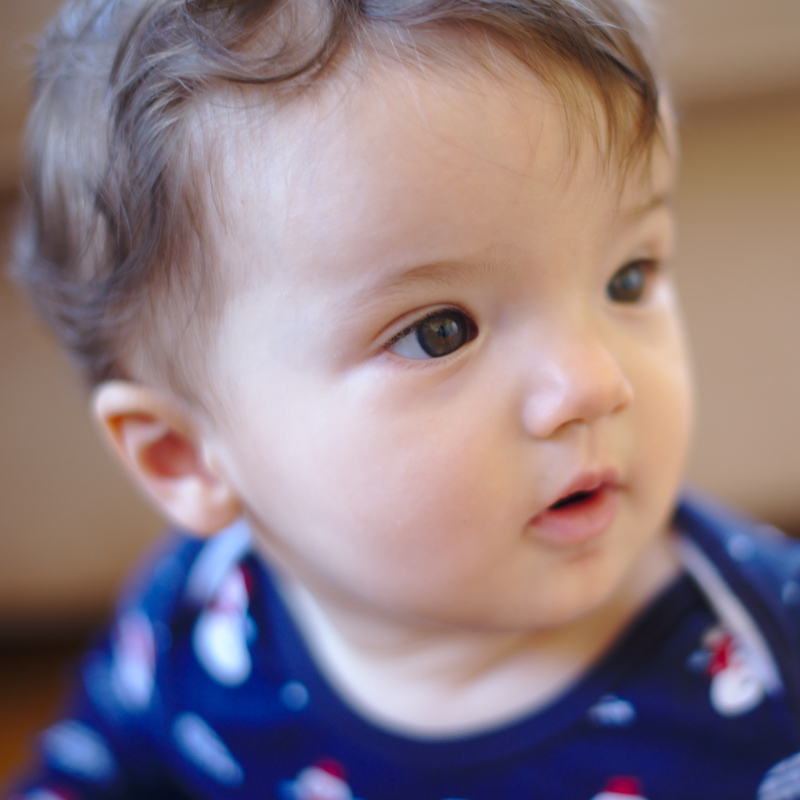
\includegraphics[width=2cm]{figures/theo6.jpg}}%
\hfill\begin{tikzpicture}
  \begin{scope}
    \node (theo1) at (0,0) {\theo};
  \end{scope}
  \draw[->,opacity=.3] (-1.2,0) -- (1.2,0);
  \draw[->,opacity=.3] (0,-1.2) -- (0,1.2);

  \begin{scope}[xshift=4cm]
  \begin{scope}
    \node[scale=2/3] at (0,0) {\theo};
    \node[minimum size={2cm+.3333em}] (theo2) at (0,0) {};
  \end{scope}
  \draw[->,opacity=.3] (-1.2,0) -- (1.2,0);
  \draw[->,opacity=.3] (0,-1.2) -- (0,1.2);
  \end{scope}

  \draw[->] (theo1.20) to["$T$", out=20, in=160] (theo2.160);

  \begin{scope}[xshift=8cm]
  \begin{scope}
    \node<4-> (theo3) at (0,0) {\theo};
  \end{scope}
  \draw<4->[->,opacity=.3] (-1.2,0) -- (1.2,0);
  \draw<4->[->,opacity=.3] (0,-1.2) -- (0,1.2);
  \end{scope}

  \draw<4->[->] (theo2.20) to["$T\inv$", out=20, in=160] (theo3.160);
  \useasboundingbox (9.2,0);
\end{tikzpicture}\hfill\null\\[1mm]
\pause
$T\inv$ is \emph{stretching} by $3/2$.

\pause\medskip
Let $T = $ projection onto the $x$-axis.  What is $T\inv$?
\pause
It is not invertible: you can't undo it.

\end{frame}


%%%%%%%%%%%%%%%%%%%%%%%%%%%%%%%%%%%%%%%%%%%%%%%%%%%%%%%%%%%%%%%%%%%

\begin{frame}
\frametitle{Invertible Linear Transformations}

If $T\colon\R^n\to\R^n$ is an invertible \emph{linear} transformation with
matrix $A$, then what is the matrix for $T\inv$?

\medskip
\begin{webonly}
Let $B$ be the matrix for $T\inv$.
We know $T\circ T\inv$ has matrix $AB$, so for all $x$,
\[ ABx = T\circ T\inv(x) = x. \]
Hence $AB = I_n$, so $B = A\inv$.
\end{webonly}

\pause\vskip 1cm
\begin{bluebox}[Fact]{.85\linewidth}
  If $T$ is an invertible linear transformation with matrix $A$, then\\[1mm]
  $T\inv$ is an invertible linear transformation with matrix $A\inv$.
\end{bluebox}

\end{frame}


%%%%%%%%%%%%%%%%%%%%%%%%%%%%%%%%%%%%%%%%%%%%%%%%%%%%%%%%%%%%%%%%%%%

\begin{frame}
\frametitle{Invertible Linear Transformations}
\framesubtitle{Examples}

\displayskips{4pt}
Let $T = $ counterclockwise rotation in the plane by $45^\circ$.  Its matrix is
\webonlycmd{
\[ A = \mat{\cos(45^\circ) -\sin(45^\circ) ; \sin(45^\circ) \cos(45^\circ)}
= \frac 1{\sqrt 2}\mat{1 -1; 1 1}. \]}%
Then $T\inv = $ counterclockwise rotation by $-45^\circ$.  Its matrix is
\webonlycmd{
\[ B = \mat{\cos(-45^\circ) -\sin(-45^\circ) ; \sin(-45^\circ) \cos(-45^\circ)}
= \frac 1{\sqrt 2}\mat{1 1; -1 1}. \]}%
\rlap{\alert{Check:}}\hfill
\webonlycmd{
$\displaystyle AB = \frac 12\mat{1 -1; 1 1}\mat{1 1; -1 1} = 
\mat{1 0 ; 0 1} \bigcheck[\quad]$}
\hfill\null

\pause\medskip
Let $T = $ shrinking by a factor of $2/3$ in the plane.  Its matrix is
\webonlycmd{
\[ A = \mat{2/3 0; 0 2/3} \]}%
Then $T\inv = $ stretching by $3/2$.  Its matrix is
\webonlycmd{
\[ B = \mat{3/2 0; 0 3/2} \]}%
\rlap{\alert{Check:}}\hfill
\webonlycmd{
$\displaystyle AB = \mat{2/3 0; 0 2/3}\mat{3/2 0; 0 3/2} = \mat{1 0; 0 1}
 \bigcheck[\quad]$}
\hfill\null

\end{frame}


%%%%%%%%%%%%%%%%%%%%%%%%%%%%%%%%%%%%%%%%%%%%%%%%%%%%%%%%%%%%%%%%%%%

\begin{frame}
\frametitle{The Invertible Matrix Theorem}
\framesubtitle{A.K.A.\ The Really Big Theorem of Math~1553}

\vskip-3mm
\begin{oneoffthm}{The Invertible Matrix Theorem}
  Let $A$ be an $n\times n$ matrix, and let $T\colon\R^n\to\R^n$ be the
  linear transformation $T(x) = Ax$.  The following statements are equivalent.
  \begin{enumerate}
  \item \namedbox{first}{$A$} is invertible.
    \pause
  \item $T$ is invertible.
    \pause
  \item $A$ is row equivalent to $I_n$.
    \pause
  \item $A$ has $n$ pivots.
    \pause
  \item $Ax=0$ has only the trivial solution.
    \pause
  \item The columns of $A$ are linearly independent.
    \pause
  \item $T$ is one-to-one.
    \pause
  \item $Ax = b$ is consistent for all $b$ in $\R^n$.
    \pause
  \item The columns of $A$ span $\R^n$.
    \pause
  \item $T$ is onto.
    \pause
  \item $A$ has a left inverse (there exists $B$ such that $BA = I_n$).
    \pause
  \item $A$ has a right inverse (there exists $B$ such that $AB = I_n$).
    \pause
  \item \namedbox{last}{$A^T$} is invertible.
  \end{enumerate}
  \pause
  \begin{tikzpicture}[remember picture, overlay]
    \draw[decorate,decoration={brace, amplitude=3mm}, thick, red]
      let \p1=($(current page.east) + (-2cm,0)$) in
        (first.north -| \p1) -- (last.south -| \p1)
        node[rotate=-90, midway, anchor=south, yshift=.2cm]
          {you really have to know these};
  \end{tikzpicture}
\end{oneoffthm}
\end{frame}


%%%%%%%%%%%%%%%%%%%%%%%%%%%%%%%%%%%%%%%%%%%%%%%%%%%%%%%%%%%%%%%%%%%

\begin{frame}
\frametitle{The Invertible Matrix Theorem}
\framesubtitle{Summary}

There are two kinds of \textcolor{red}{\emph{square}} matrices:
\pause
\begin{enumerate}
\item invertible (non-singular), and
\pause
\item non-invertible (singular).
\end{enumerate}

\pause\bigskip
For invertible matrices, all statements of the Invertible Matrix Theorem are true.

\pause\bigskip
For non-invertible matrices, all statements of the Invertible Matrix Theorem are
false.

\pause\bigskip
\alert{Strong recommendation:} 
If you want to understand invertible matrices, go through all of the conditions
of the IMT and try to figure out on your own (or at least with help from the
book) why they're all equivalent.

\pause\bigskip
You know enough at this point to be able to reduce all of the statements to
assertions about the pivots of a square matrix.

\end{frame}


%%% Local Variables:
%%% TeX-master: "../slides"
%%% End:

% 
% JDR: This should take a bit more than one lecture as written.  It can bleed
%   into 2.9, which is shorter.

\titleframe{Section 2.8}{Subspaces of $\R^n$}


%%%%%%%%%%%%%%%%%%%%%%%%%%%%%%%%%%%%%%%%%%%%%%%%%%%%%%%%%%%%%%%%%%%

\begin{frame}
\frametitle{Motivation}

Today we will discuss \textbf{subspaces} of $\R^n$.

\pause\medskip
A subspace turns out to be the same as a span, except we don't know \emph{which}
vectors it's the span of.

\pause\medskip
This arises naturally when you have, say, a plane through the origin in $\R^3$
which is \emph{not} defined (a priori) as a span, but you still want to say
something about it.

\begin{center}
\begin{tikzpicture}[myxyz, scale=.6]
  \def\v{(2,-1,1)}
  \def\w{(1,0,-1)}

  \node[coordinate] (X) at \v {};
  \node[coordinate] (Y) at \w {};

  \begin{scope}[x=(X), y=(Y), transformxy]
    \fill[seq4!30, nearly opaque] (-1.5,-2) rectangle (1.5,2);
    \draw[step=.5cm, seq4!50, very thin] (-1.5,-2) grid (1.5,2);
  \end{scope}

  \node[seq4] at (-2.5cm, 2.9cm) {$x+3y+z=0$};

  \point at (0,0,0);
\end{tikzpicture}
\end{center}
\end{frame}


%%%%%%%%%%%%%%%%%%%%%%%%%%%%%%%%%%%%%%%%%%%%%%%%%%%%%%%%%%%%%%%%%%%

\begin{frame}
\frametitle{Definition of Subspace}

\vskip-3mm
\begin{defn}
  A \textbf{subspace} of $\R^n$ is a subset $V$ of $\R^n$ satisfying:
  \begin{enumerate}
  \item The zero vector is in $V$.
    \hfill \pause\textcolor{blue}{``not empty''}
    \pause
  \item If $u$ and $v$ are in $V$, then $u+v$ is also in $V$.
    \hfill \pause\textcolor{blue}{``closed under addition''}
    \pause
  \item If $u$ is in $V$ and $c$ is in $\R$, then $cu$ is in $V$.
    \hfill \pause\textcolor{blue}{``closed under $\times$ scalars''}
  \end{enumerate}
\end{defn}
\note{(3) doesn't imply (1): could be empty}

\pause\medskip
\alert{What does this mean?}
\begin{itemize}
\item If $v$ is in $V$, then all scalar multiples of $v$ are in $V$ by~(3).
  \pause
  That is, the line through $v$ is in $V$.

  \pause
\item If $u,v$ are in $V$, then $xu$ and $yv$ are in $V$ for scalars $x,y$ by~(3).
  \pause
  So $xu+yv$ is in $V$ by~(2).
  \pause
  So $\Span\{u,v\}$ is contained in $V$.

  \pause
\item Likewise, if $v_1,v_2,\ldots,v_n$ are all in $V$, then 
  $\Span\{v_1,v_2,\ldots,v_n\}$ is contained in $V$.

\end{itemize}

\pause\medskip
\begin{bluebox}{.75\linewidth}
  A subspace $V$ contains the span of any set of vectors in $V$.
\end{bluebox}

\end{frame}


%%%%%%%%%%%%%%%%%%%%%%%%%%%%%%%%%%%%%%%%%%%%%%%%%%%%%%%%%%%%%%%%%%%

\begin{frame}
\frametitle{Examples}

\vskip-3mm
\begin{eg}
  \begin{minipage}[t]{.5\linewidth}
    A line $L$ through the origin: this contains the span of any vector in $L$.
  \end{minipage}\hfill
  \begin{tikzpicture}[scale=.5, baseline]
    \useasboundingbox (-3,-1) -- (3,0);
    \draw[seq4] (-3,-1) -- (3,1);
    \draw[vector] (0,0) -- (1,1/3);
    \point at (0,0);
    \node[seq4] at (0,.5) {$L$};
  \end{tikzpicture}
\end{eg}

\pause
\begin{eg}
  \begin{minipage}[t]{.5\linewidth}
    A plane $P$ through the origin: this contains the span of any vectors in $P$.
  \end{minipage}\hfill
  \begin{tikzpicture}[myxyz, scale=.5, baseline=.5cm]
    \useasboundingbox[resetxy] (-3,-3) rectangle (3,0);
  
    \def\v{(2,-1,1)}
    \def\w{(1,0,-1)}
  
    \node[coordinate] (X) at \v {};
    \node[coordinate] (Y) at \w {};
  
    \begin{scope}[x=(X), y=(Y), transformxy]
      \fill[seq4!30, nearly opaque] (-1,-1) rectangle (1,1);
      \draw[step=.5cm, seq4!50, very thin] (-1,-1) grid (1,1);
    \end{scope}

    \draw[vector] (0,0,0) -- ($.5*(X)$);
    \draw[vector] (0,0,0) -- ($.5*(Y)$);
  
    \point at (0,0,0);
    \node[x=(X),y=(Y),seq4] at (.2,-1.4) {$P$};
  \end{tikzpicture}
\end{eg}

\pause
\begin{eg}
  All of $\R^n$: this contains $0$, and is closed under addition and scalar
  multiplication.
\end{eg}

\pause
\begin{eg}
  The subset $\{0\}$: this subspace contains only one vector.
\end{eg}

\pause\medskip
Note these are all pictures of spans!  (Line, plane, space, etc.)

\end{frame}


%%%%%%%%%%%%%%%%%%%%%%%%%%%%%%%%%%%%%%%%%%%%%%%%%%%%%%%%%%%%%%%%%%%

\begin{frame}
\frametitle{Non-Examples}

\vskip-3mm
\begin{noneg}
  \begin{minipage}[t]{.5\linewidth}
    A line $L$ (or any other set) that doesn't contain the origin is not a
    subspace.  Fails: \uncover<2->{\alert 1.}
  \end{minipage}\hfill
  \begin{tikzpicture}[scale=.5, baseline]
    \useasboundingbox (-3,-1) -- (3,0);
    \draw[seq4] (-3,-1) -- (3,1);
    \point<1> at (0,-.5);
    \point<2->[red] at (0,-.5);
  \end{tikzpicture}\hskip 0pt plus .5fill\null
\end{noneg}

\pause[3]%
\begin{noneg}
  \begin{minipage}[t]{.5\linewidth}
    A circle $C$ is not a subspace.  Fails: \uncover<4->{\alert{1,2,3}.}
    \uncover<5->{Think: a circle isn't a ``linear space.''}
  \end{minipage}\hfill
  \begin{tikzpicture}[scale=.5, baseline]
    \useasboundingbox (-2,-2) -- (2,0);
    \draw[seq4] (0,0) circle [radius=2cm];
    \draw<4->[vector,red] (0,0) -- (2.5,0);
    \draw<4->[vector] (0,0) -- (0,2);
    \draw<4->[vector] (0,0) -- (2,0);
    \draw<4->[vector,red] (0,0) -- (2,2);
    \point<3> at (0,0);
    \point<4->[red] at (0,0);
  \end{tikzpicture}\hskip 0pt plus .5fill\null
\end{noneg}

\pause[6]%
\begin{noneg}
  \begin{minipage}[t]{.5\linewidth}
    The first quadrant in $\R^2$ is not a subspace.
    Fails: \uncover<7->{\alert{3} only.}
  \end{minipage}\hfill
  \begin{tikzpicture}[scale=.5, baseline]
    \useasboundingbox (-2,-2) -- (2,1);
    \fill[seq4!20] (0,0) rectangle (2,2);
    \draw[->] (-2,0) -- (2,0);
    \draw[->] (0,-2) -- (0,2);
    \draw<7->[vector] (0,0) -- (1,1);
    \draw<7->[vector,red] (0,0) -- (-1,-1);
    \point at (0,0);
  \end{tikzpicture}\hskip 0pt plus .5fill\null
\end{noneg}

\pause[8]%
\begin{noneg}
  \begin{minipage}[t]{.5\linewidth}
    A line union a plane in $\R^3$ is not a subspace.
    Fails: \uncover<9->{\alert{2} only.}
  \end{minipage}\hfill
  \begin{tikzpicture}[scale=.5, baseline, myxyz]
    \useasboundingbox (-4,-2) -- (4,1);
    \path[clip, resetxy] (-4,-2) rectangle (4,2);
  
    \draw[seq4] (-1,-2,-4) -- (0,0,0);

    \begin{scope}[transformxy]
      \fill[seq4!20, semitransparent] (-1.5,-1.5) rectangle (1.5,1.5);
      \draw[step=.5cm, grid lines] (-1.5,-1.5) grid (1.5,1.5);
    \end{scope}
  
    \draw[seq4] (1,2,4) -- (0,0,0);

    \draw<9->[vector] (0,0,0) -- (.3,.6,1.2);
    \draw<9->[vector] (0,0,0) -- (1,0,0);
    \draw<9->[vector,red] (0,0,0) -- (1.3,.6,1.2);

    \point at (0,0,0);

  \end{tikzpicture}\hskip 0pt plus .5fill\null
\end{noneg}

\end{frame}


%%%%%%%%%%%%%%%%%%%%%%%%%%%%%%%%%%%%%%%%%%%%%%%%%%%%%%%%%%%%%%%%%%%

\begin{frame}
\frametitle{Subsets and Subspaces}
\framesubtitle{They aren't the same thing}

A \textbf{subset} of $\R^n$ is any collection of vectors whatsoever.

\pause\bigskip
All of the non-examples are still subsets.

\pause\bigskip
A \textbf{subspace} is a special kind of subset, which satisfies the three
defining properties.

\pause\vskip 1cm\hfill
\begin{tikzpicture}[scale=.5, baseline]
  \draw[grid lines] (-2.5,-2.5) grid (2.5,2.5);
  \draw (0,0) circle [radius=2cm];
\end{tikzpicture}
\quad
\begin{minipage}{.5\linewidth}\leavevmode
\hbox to 1.5cm{Subset:\hss} \emph{yes}\\
\hbox to 1.5cm{Subspace:\hss} \emph{no}
\end{minipage}\hfill\null

\end{frame}


%%%%%%%%%%%%%%%%%%%%%%%%%%%%%%%%%%%%%%%%%%%%%%%%%%%%%%%%%%%%%%%%%%%

\begin{frame}
\frametitle{Spans are Subspaces}

\vskip-3mm
\begin{thm}
  Any $\Span\{v_1,v_2,\ldots,v_n\}$ is a subspace.
\end{thm}

\pause\medskip
\begin{bluebox}[!!!]{.7\linewidth}
  Every subspace is a span, and every span is a subspace.
\end{bluebox}

\pause
\begin{defn}
  If $V = \Span\{v_1,v_2,\ldots,v_n\}$, we say that $V$ is the
  subspace \textbf{generated by} or \textbf{spanned by}
  the vectors $v_1,v_2,\ldots,v_n$.
\end{defn}

\medskip
\begin{webonly}
\alert{Check:}
\begin{enumerate}
\item $0 = 0v_1 + 0v_2 + \cdots + 0v_n$ is in the span.
\item If, say, $u = 3v_1 + 4v_2$ and $v = -v_1 - 2v_2$, then
  \[ u + v = 3v_1 + 4v_2 -v_1 - 2v_2 = 2v_1 + 2v_2 \]
  is also in the span.
\item Similarly, if $u$ is in the span, then so is $cu$ for any scalar $c$.
\end{enumerate}
\end{webonly}

\end{frame}


%%%%%%%%%%%%%%%%%%%%%%%%%%%%%%%%%%%%%%%%%%%%%%%%%%%%%%%%%%%%%%%%%%%

\begin{pollframe}

\begin{poll}
\vfill

\begin{bluebox}[Poll]{.9\linewidth}
  Is the empty set $\{\}$ a subspace?  If not, which property(ies) does it fail?
\end{bluebox}

\pause\medskip
The zero vector is not contained in the empty set, so it is \emph{not} a
subspace.
\end{poll}

\pause\bigskip
\alert{Question:} What is the difference between $\{\}$ and $\{0\}$?

\vfill

\end{pollframe}


%%%%%%%%%%%%%%%%%%%%%%%%%%%%%%%%%%%%%%%%%%%%%%%%%%%%%%%%%%%%%%%%%%%

\begin{frame}
\frametitle{Subspaces}
\framesubtitle{Verification}

Let $V = \left\{ \vec{a b} \text{ in } \R^2\bigm| ab=0 \right\}$.  Let's check
if $V$ is a subspace or not.

\begin{webonly}
\begin{enumerate}
\item Does $V$ contain the zero vector?
  ${a\choose b} = {0\choose 0} \implies ab = 0$ \bigcheck[\quad]
\item[3.] Is $V$ closed under scalar multiplication?
  \begin{itemize}
  \item Let $a\choose b$ be in $V$.  
  \item \emph{This means:} $a$ and $b$ are numbers such that $ab=0$.
  \item Let $c$ be a scalar.  Is $c{a\choose b} = {ca\choose cb}$ in $V$?
  \item \emph{This means:} $(ca)(cb) = 0$.  
  \item Well, $(ca)(cb) = c^2(ab) = c^2(0) = 0 \bigcheck[\quad]\namedbox{mark}{}$
  \end{itemize}
\item[2.] Is $V$ closed under addition?
  \begin{itemize}
  \item Let $a\choose b$ and $a'\choose b'$ be in $V$.  
  \item \emph{This means:} $ab = 0$ and $a'b' = 0$.
  \item Is ${a\choose b} + {a'\choose b'} = {a+a'\choose b+b'}$ in $V$?
  \item \emph{This means:} $(a+a')(b+b')=0$.
  \item This is not true for all such $a,a',b,b'$: for instance,
    $1\choose 0$ and $0\choose 1$ are in $V$, but their sum 
    ${1\choose 0} + {0\choose 1} = {1\choose 1}$ is not in $V$, because
    $1\cdot 1\neq 0$. \bigcross
  \end{itemize}
\end{enumerate}
\end{webonly}

\pause
We conclude that $V$ is \emph{not} a subspace.
\pause
A picture is above.  (It doesn't look like a span.)
\begin{tikzpicture}[remember picture, overlay]
  \begin{scope}[shift=(mark), xshift=3.5cm]
    \draw[grid lines, step=.25] (-1,-1) grid (1,1);
    \draw[seq4, <->] (-1,0) -- (1,0);
    \draw[seq4, <->] (0,-1) -- (0,1);
    \node[seq4] at (.25,.25) {$V$};
  \end{scope}
\end{tikzpicture}

\end{frame}


%%%%%%%%%%%%%%%%%%%%%%%%%%%%%%%%%%%%%%%%%%%%%%%%%%%%%%%%%%%%%%%%%%%

\begin{frame}
\frametitle{Column Space and Null Space}

An $m\times n$ matrix $A$ naturally gives rise to \emph{two}
subspaces.

\pause
\begin{defn}
  \begin{itemize}
  \item The \textbf{column space} of $A$ is the subspace of
    $\R^{\blankuntil{3}{m}}$ spanned by the columns of $A$.  It is written 
    $\Col A$.
    \pause[4]
  \item The \textbf{null space} of $A$ is the set of all solutions of the
    homogeneous equation $Ax=0$:
    \[ \Nul A = \bigl\{ x \text{ in } \R^{\blankuntil{5}{n}}\mid Ax=0 \bigr\}. \]
    This is a subspace of $\R^{\blankuntil{5}{n}}$.
  \end{itemize}
\end{defn}

\vskip -.1cm
\pause[6]
The column space is defined as a span, so we know it is a subspace.
\pause
It is the range (as opposed to the codomain) of the transformation $T(x) = Ax$.

\pause\medskip
\alert{Check} that the null space is a subspace:
\begin{webonly}
\begin{enumerate}
\item $0$ is in $\Nul A$ because $A0 = 0$.
\item If $u$ and $v$ are in $\Nul A$, then $Au = 0$ and $Av = 0$.  Hence
  \abovedisplayskip=1pt\belowdisplayskip=1pt
  \[ A(u+v) = Au + Av = 0, \]
  so $u+v$ is in $\Nul A$.
\item If $u$ is in $\Nul A$, then $Au = 0$.  For any scalar $c$,
  $A(cu) = cAu = 0$.  So $cu$ is in $\Nul A$.
\end{enumerate}
\end{webonly}

\end{frame}


%%%%%%%%%%%%%%%%%%%%%%%%%%%%%%%%%%%%%%%%%%%%%%%%%%%%%%%%%%%%%%%%%%%

\begin{frame}
\frametitle{Column Space and Null Space}
\framesubtitle{Example}

Let $A = \mat{1 1; 1 1; 1 1}$.

\medskip
\begin{minipage}{.7\linewidth}
Let's compute the column space:
\begin{webonly}
\[ \Col A = \Span\left\{\vec{1 1 1},\,\vec{1 1 1}\right\}
= \Span\left\{\vec{1 1 1}\right\}. \]
This is a line in $\R^3$.
\end{webonly}
\end{minipage}\hfill\pause
\begin{tikzpicture}[scale=.5, baseline, myxyz]
  \useasboundingbox (-4,-2) -- (4,1);
  \path[clip, resetxy] (-4,-2) rectangle (4,2);

  \draw[seq4] (-4,-4,-4) -- (0,0,0);
   \begin{scope}[transformxy]
    \fill[white, semitransparent] (-1.5,-1.5) rectangle (1.5,1.5);
    \draw[step=1cm, grid lines] (-1.5,-1.5) grid (1.5,1.5);
  \end{scope}

  \draw[seq4] (4,4,4) -- (0,0,0);
  \draw[vector] (0,0,0) -- (1,1,1);
  \draw[densely dotted] (1,1,0) -- (1,1,1);
  \node[resetxy,seq4] at (1.5,1.5) {$\Col A$};
  \point at (0,0,0);
\end{tikzpicture}

\bigskip

\begin{minipage}{.7\linewidth}
\pause
Let's compute the null space:
\begin{webonly}
\displayskips{1pt}
\[ A\vec{x y} = \vec{x+y x+y x+y}. \]
This zero if and only if $x=-y$.  So
\[ \Nul A = \left\{ \vec{x y}\text{ in }\R^2\mid y=-x \right\}. \]
This defines a line in $\R^2$:
\end{webonly}
\end{minipage}
\hfill\pause
\begin{tikzpicture}[scale=.5, baseline]
  \useasboundingbox (-3,-3) -- (3,1);
  \draw[grid lines] (-3,-3) grid (3,3);
  \draw[seq4] (3,-3) -- (-3,3);
  \point at (0,0);
  \node[seq4,fill=white, inner sep=1pt] at (-.7,2) {$\Nul A$};
\end{tikzpicture}

\end{frame}


%%%%%%%%%%%%%%%%%%%%%%%%%%%%%%%%%%%%%%%%%%%%%%%%%%%%%%%%%%%%%%%%%%%

\begin{frame}
\frametitle{The Null Space is a Span}

The column space of a matrix $A$ is defined to be a span (of the columns).

\pause\medskip
The null space is defined to be the solution set to $Ax=0$.
\pause
It is a subspace, so it is a span.

\pause
\begin{ques}
  How to find vectors which span the null space?
\end{ques}

\pause
\alert{Answer:} Parametric vector form!
\pause
We know that the solution set to $Ax=0$ has a parametric form that looks like
\[ x_3\vec{1 2 1 0} + x_4\vec{-2 3 0 1}\quad
\parbox{2.5cm}{\centering if, say, $x_3$ and $x_4$ are the free variables. \pause So}
\quad
\Nul A = \Span\left\{ \vec{1 2 1 0},\, \vec{-2 3 0 1} \right\}.
\]

\pause\medskip
Refer back to the slides for \S1.5 (Solution Sets).

\pause\medskip
\alert{Note:} It is much easier to define the null space first as a
subspace, then find spanning vectors \emph{later}, if we need them.  This is one
reason subspaces are so useful.

\end{frame}


%%%%%%%%%%%%%%%%%%%%%%%%%%%%%%%%%%%%%%%%%%%%%%%%%%%%%%%%%%%%%%%%%%%

\begin{frame}
\frametitle{The Null Space is a Span}
\framesubtitle{Example, revisited}

Find vector(s) that span the null space of $A = \mat{1 1; 1 1; 1 1}$.

\begin{webonly}
\medskip
The reduced row echelon form is
$\mat{1 1; 0 0; 0 0}$.

\medskip
This gives the equation $x + y = 0$, or
\[ \syseq{x = -y; y = y}
\quad\longsquiggly[parametric vector form]\quad
\vec{x y} = y\vec{-1 1}. \]
\end{webonly}

\begin{minipage}[t]{.6\linewidth}
  \webonlycmd{
  The null space is
  \[ \Nul A = \Span\left\{ \vec{-1 1} \right\}. \]}
\end{minipage}\pause
\begin{tikzpicture}[scale=.5, baseline=1cm]
  \draw[grid lines] (-3,-3) grid (3,3);
  \draw[seq4] (3,-3) -- (-3,3);
  \draw[vector] (0,0) -- (-1,1);
  \point at (0,0);
  \node[seq4,fill=white, inner sep=1pt] at (-.7,2) {$\Nul A$};
  \end{tikzpicture}

\end{frame}


%%%%%%%%%%%%%%%%%%%%%%%%%%%%%%%%%%%%%%%%%%%%%%%%%%%%%%%%%%%%%%%%%%%

\begin{frame}
\frametitle{Subspaces}
\framesubtitle{Summary}

\vskip 5mm

\begin{bluebox}[How do you check if a subset is a subspace?]{.9\linewidth}
  \smallskip
  \begin{itemize}
  \item<+-> Is it a span?  Can it be written as a span?
  \item<+-> Can it be written as the column space of a matrix?
  \item<+-> Can it be written as the null space of a matrix?
  \item<+-> Is it all of $\R^n$ or the zero subspace $\{0\}$?
  \item<+-> Can it be written as a type of subspace that we'll learn about later
    (eigenspaces, \ldots)?
  \end{itemize}

  \smallskip\uncover<+->{%
  If so, then it's automatically a subspace.}

  \smallskip\uncover<+->{%
  If all else fails:}
  \begin{itemize}
  \item<+-> Can you verify directly that it satisfies the three defining
    properties?
  \end{itemize}
\end{bluebox}

\end{frame}


%%%%%%%%%%%%%%%%%%%%%%%%%%%%%%%%%%%%%%%%%%%%%%%%%%%%%%%%%%%%%%%%%%%

\begin{frame}
\frametitle{Basis of a Subspace}

What is the \emph{smallest number} of vectors that are needed to span a subspace?

\pause\bigskip
\namedbox{basis}{%
\begin{minipage}{\textwidth}\vskip -.14cm
\begin{defn}
  Let $V$ be a subspace of $\R^n$.  A \textbf{basis} of $V$ is a set of vectors
  $\{v_1,v_2,\ldots,v_m\}$ in $V$ such that:
  \begin{enumerate}
    \pause
  \item $V = \Span\{v_1,v_2,\ldots,v_m\}$, and
    \pause
  \item $\{v_1,v_2,\ldots,v_m\}$ is linearly independent.
  \end{enumerate}
  \pause
  The number of vectors in a basis is the \textbf{dimension} of $V$, and is
  written $\dim V$.
\end{defn}
\end{minipage}
}
\begin{tikzpicture}[remember picture, overlay]
  \node<6->[redbox, fit=(basis)] (basisbox) {};
  \node<6->[red, rotate=-90, anchor=south, font=\small, text width=2cm, align=center]
    at (basisbox.east) {Note the big red border here};
\end{tikzpicture}

\begin{uncoverenv}<7->
\pause[7]\bigskip
\alert{Why} is a basis the smallest number of vectors needed to span?

\pause\medskip
Recall: \emph{linearly independent} means that every time you add another
vector, the span gets bigger.

\pause\medskip
Hence, if we remove any vector, the span gets \emph{smaller\/}: so any smaller set
can't span $V$.

\pause
\begin{bluebox}[Important]{.8\textwidth}
  A subspace has \emph{many different} bases, but they all have the same
  number of vectors (see the exercises in \S2.9).
\end{bluebox}

\end{uncoverenv}

\end{frame}


%%%%%%%%%%%%%%%%%%%%%%%%%%%%%%%%%%%%%%%%%%%%%%%%%%%%%%%%%%%%%%%%%%%

\begin{frame}
\frametitle{Bases of $\R^2$}

\vskip-.2cm
\begin{ques}
  What is a basis for $\R^2$?
\end{ques}

\begin{minipage}[t]{.6\linewidth}
  \uncover<2->{We need two vectors that \emph{span $\R^2$} and are
  \emph{linearly independent}.}
  \uncover<3->{$\{e_1,e_2\}$ is one basis.}
  \begin{enumerate}
  \item<4-> They span: ${a\choose b} =\uncover<5->{ae_1 + be_2.}$
  \item<6-> They are linearly independent because they are not collinear.
  \end{enumerate}
\end{minipage}
\hfill
\begin{uncoverenv}<3->
\begin{tikzpicture}[picture align top, scale=.75]
  \useasboundingbox (-2,-2) rectangle (2,1);
  \draw[grid lines] (-2,-2) grid (2,2);
  \draw[thick vector] (0,0) -- (1,0) node[anchor=west,whitebg] {$e_1$};
  \draw[thick vector] (0,0) -- (0,1) node[anchor=south,whitebg] {$e_2$};
  \point at (0,0);
\end{tikzpicture}
\end{uncoverenv}

\pause[7]\smallskip
\begin{ques}
  What is another basis for $\R^2$?
\end{ques}

\begin{minipage}[t]{.6\linewidth}
  \uncover<8->{Any two nonzero vectors that are not collinear.}
  \uncover<9->{$\bigl\{{1\choose 0},{1\choose 1}\bigr\}$ is also a basis.}
  \begin{enumerate}
  \item<10-> They span: $\begin{psmm}1&1\\0&1\end{psmm}$ has a pivot in every row.
  \item<11-> They are linearly independent: $\begin{psmm}1&1\\0&1\end{psmm}$ has
    a pivot in every column.
  \end{enumerate}
\end{minipage}
\hfill
\begin{uncoverenv}<9->
\begin{tikzpicture}[picture align top, scale=.75]
  \useasboundingbox (-2,-2) rectangle (2,1);
  \draw[grid lines] (-2,-2) grid (2,2);
  \draw[thick vector] (0,0) -- (1,0) node[anchor=west,whitebg] {$1\choose 0$};
  \draw[thick vector] (0,0) -- (1,1) node[anchor=south,whitebg] {$1\choose 1$};
  \point at (0,0);
\end{tikzpicture}
\end{uncoverenv}

\end{frame}


%%%%%%%%%%%%%%%%%%%%%%%%%%%%%%%%%%%%%%%%%%%%%%%%%%%%%%%%%%%%%%%%%%%

\begin{frame}
\frametitle{Bases of $\R^n$}

The unit coordinate vectors
\[ e_1 = \vec{1 0 \vdots, 0 0},\quad e_2 = \vec{0 1 \vdots, 0 0},\quad\ldots,\quad
   e_{n-1} = \vec{0 0 \vdots, 1 0},\quad e_n = \vec{0 0 \vdots, 0 1} \]
are a basis for $\R^n$.
\pause
\begin{enumerate}
\item They span: \namedbox{identity}{$I_n$} has a pivot in every row.
\pause
\begin{tikzpicture}[blue!50, remember picture, overlay]
  \path (identity.north) ++(1cm,.25cm)
    node[font=\small, anchor=west] (expl)
      {The identity matrix has columns $e_1,e_2,\ldots,e_n$.};
  \draw[->, shorten >=1pt] (expl.west) to[out=180,in=90] (identity.north);
\end{tikzpicture}
\pause
\item They are linearly independent: $I_n$ has a pivot in every column.
\end{enumerate}

\pause\medskip
\alert{In general:} $\{v_1,v_2,\ldots,v_n\}$ is a basis for $\R^n$ if and only
if the matrix 
\[ A = \mat{| | ,, |; v_1 v_2 \cdots, v_n; | | ,, |} \]
has a pivot in every row and every column,
i.e.\ if $A$ is \blankuntil{6}{\emph{invertible}}.

\end{frame}


%%%%%%%%%%%%%%%%%%%%%%%%%%%%%%%%%%%%%%%%%%%%%%%%%%%%%%%%%%%%%%%%%%%

\begin{frame}
\frametitle{Basis of a Subspace}
\framesubtitle{Example}

\vskip-3mm
\begin{eg}
  Let\vskip-7mm
  \[ V = \left\{ \vec{x y z} \text{ in } \R^3\bigm| x + 3y + z = 0 \right\} \qquad 
  \cB = \left\{ \vec{-3 1 0},\;\vec{0 1 -3} \right\}. \]
  Verify that $\cB$ is a basis for $V$.

  \begin{webonly}
    \displayskips{3pt}
  \begin{enumerate}\setcounter{enumi}{-1}
  \item \alert{In $V$:} both vectors are in $V$ because
    \[ -3 + 3(1) + 0 = 0 \sptxt{and} 0 + 3(1) + (-3) = 0. \]
    
  \item \alert{Span:}
    If $\vec{x y z}$ is in $V$, then $y = -\frac 13(x+z)$, so
    \vskip-3mm
    \[ \vec{x y z} = -\frac x3\vec{-3 1 0} - \frac z3\vec{0 1 -3}. \]
    
  \item \alert{Linearly independent:}
    \[ c_1\vec{-3 1 0} + c_2\vec{0 1 -3} = 0
    \implies \vec{-3c_1 c_1+c_2 -3c_2} = \vec{0 0 0}
    \implies c_1 = c_2 = 0. \]
  \end{enumerate}
  \end{webonly}
\end{eg}

\end{frame}


%%%%%%%%%%%%%%%%%%%%%%%%%%%%%%%%%%%%%%%%%%%%%%%%%%%%%%%%%%%%%%%%%%%

\begin{frame}
\frametitle{Basis for $\Nul A$}

\begin{bluebox}[Fact]{.8\linewidth}
  The vectors in the parametric vector form of the general
  solution to $Ax=0$ always form a basis for $\Nul A$.
\end{bluebox}

\pause
\begin{eg}
  \vskip-6mm
  \begin{webonly}
  \[\begin{split}
    A &= \mat[r]{1 2 0 -1; -2 -3 4 5; 2 4 0 -2}
      \quad\longsquiggly[rref]\quad
      \mat[r]{1 0 -8 -7; 0 1 4 3; 0 0 0 0} \\
    &\quad
      \longsquiggly[\parbox{\widthof{parametric}}
        {\centering parametric\\vector\\[-2pt]form}]
    \quad \namedbox{x}{x} {}= x_3\vec{8 -4 1 0} + x_4\vec{7 -3 0 1} 
      \;\longsquiggly[\parbox{\widthof{basis of}}{
        \centering basis of\\$\Nul A$\strut}]\;
      \left\{ \vec{8 -4 1 0},\,\vec{7 -3 0 1} \right\}
  \end{split}\]
  \begin{enumerate}
  \item The vectors span $\Nul A$ by construction (every solution to $Ax=0$
    has \namedbox{this}{this} form).
    \tikz[remember picture, overlay, blue!50]
      \draw[->, shorten >=1pt]
        (this.north) .. controls ++(0,1) and ++(0,-2) .. (x.south);
  \item Can you see why they are linearly independent?
    (Look at the last two rows.)
  \end{enumerate}
  \end{webonly}
\end{eg}

\end{frame}


%%%%%%%%%%%%%%%%%%%%%%%%%%%%%%%%%%%%%%%%%%%%%%%%%%%%%%%%%%%%%%%%%%%

\begin{frame}
\frametitle{Basis for $\Col A$}

\begin{bluebox}[Fact]{.8\textwidth}
  The \emph{pivot columns} of $A$ always form a basis for $\Col A$.
\end{bluebox}

\pause\medskip
\alert{Warning:} I mean the pivot columns of the \emph{original} matrix $A$, not
the row-reduced form.
\pause
(Row reduction changes the column space.)

\pause
\begin{eg}\vskip-5mm
  \begin{webonly}
  \[ A = \mat[r]{\namedbox{col1top}{1} \namedbox{col2top}{2} 0 -1; -2 -3 4 5;
    \namedbox{col1bot}{2} \namedbox{col2bot}{4} 0 -2}
  \quad\longsquiggly[rref]\quad
  \mat[r]{1 0 -8 -7; 0 1 4 3; \namedbox{rcol1}{0} \namedbox{rcol2}{0} 0 0} \]
  \begin{tikzpicture}[remember picture, overlay]
    \path ($(rcol1)!.5!(rcol2)$) ++(0,-1cm)
      node[blue!50, font=\small] (rref) {pivot columns in rref};
    \draw[->,blue!50, shorten >=1pt] (rref.north) to[out=90,in=-90] (rcol1.south);
    \draw[->,blue!50, shorten >=1pt] (rref.north) to[out=90,in=-90] (rcol2.south);
  \end{tikzpicture}
  \begin{tikzpicture}[remember picture, overlay]
    \path let \p1=($(col1bot)!.5!(col2bot)$) in (\p1 |- rref.base)
      node[blue!50, font=\small,anchor=base] (orig) {pivot columns $=$ basis};
    \node[fit=(col1top) (col1bot), draw=orange, rounded corners] (col1) {};
    \node[fit=(col2top) (col2bot), draw=orange, rounded corners] (col2) {};
    \draw[->,blue!50, shorten >=1pt] (orig.north) to[out=90,in=-90] (col1.south);
    \draw[->,blue!50, shorten >=1pt] (orig.north) to[out=90,in=-90] (col2.south);
    \draw[->,
        decoration={snake, amplitude=.4mm, segment length=1mm, post length=.5mm},
        decorate]
      (rref.west) -- (orig.east);
  \end{tikzpicture}

  \vskip 1cm
  So a basis for $\Col A$ is 
  \[ \left\{ \vec[r]{1 -2 2},\,\vec[r]{2 -3 4} \right\}. \]
  \end{webonly}
\end{eg}

\pause
\alert{Why?}  End of \S2.8, or ask in office hours.

\end{frame}


%%% Local Variables:
%%% TeX-master: "../slides"
%%% End:

% 
% JDR: This should take a bit less than one lecture as written.

\usetikzlibrary{matrix}

\titleframe{Section 2.9}{Dimension and Rank}


%%%%%%%%%%%%%%%%%%%%%%%%%%%%%%%%%%%%%%%%%%%%%%%%%%%%%%%%%%%%%%%%%%%

\begin{frame}
\frametitle{Coefficients of Basis Vectors}

\alert{Recall:} a \textbf{basis} of a subspace $V$ is a set of vectors that
\emph{spans} $V$ and is \emph{linearly independent}.

\pause
\begin{oneoffthm}{\namedbox{lemma}{Lemma}}
  \begin{tikzpicture}[remember picture, overlay]
    \path (lemma.north east) ++(1,0)
      node[anchor=west, blue!50, font=\small\upshape] (expl)
        {like a theorem, but less important};
    \draw[->, shorten >=1pt, blue!50]
      (expl.west) to[out=180,in=0] (lemma.east);
  \end{tikzpicture}%
  \pause
  If $\cB = \{v_1,v_2,\ldots,v_m\}$ is a basis for a subspace $V$, then any
  vector $x$ in $V$ can be written as a linear combination
  \[ x = c_1v_1 + c_2v_2 + \cdots + c_mv_m \]
  for \emph{unique} coefficients $c_1,c_2,\ldots,c_m$.
\end{oneoffthm}

\begin{webonly}
We know $x$ is a linear combination of the $v_i$ because they span $V$.
Suppose that we can write $x$ as a linear combination with different
coefficients:
\[\begin{split}
  x &= c_1v_1 + c_2v_2 + \cdots + c_mv_m \\
  x &= c_1'v_1 + c_2'v_2 + \cdots + c_m'v_m
\end{split}\]
Subtracting:
\[ 0 = x-x = (c_1-c_1')v_1 + (c_2-c_2')v_2 + \cdots + (c_m-c_m')v_m \]
Since $v_1,v_2,\ldots,v_m$ are linearly independent, they only have the trivial
linear dependence relation.
That means each $c_i-c_i'=0$, or $c_i=c_i'$.
\end{webonly}

\end{frame}


%%%%%%%%%%%%%%%%%%%%%%%%%%%%%%%%%%%%%%%%%%%%%%%%%%%%%%%%%%%%%%%%%%%

\begin{frame}
\frametitle{Bases as Coordinate Systems}

The unit coordinate vectors $e_1,e_2,\ldots,e_n$ form a basis
for $\R^n$.  Any vector is a unique linear combination of the $e_i$:
\[ v = \vec{\color<2->{seq1}3 \color<2->{seq2}5 \color<2->{seq3}{-2}}
= 3\vec{1 0 0} + 5\vec{0 1 0} - 2\vec{0 0 1}
= \textcolor<2->{seq1}{3}e_1 + \textcolor<2->{seq2}{5}e_2
\textcolor<2->{seq3}{{}- 2}e_3. \]

\pause
\alert{Observe:}
the \emph{coordinates} of $v$ are exactly the \emph{coefficients} of
$e_1,e_2,e_3$.

\pause\medskip
We can go backwards: given any basis $\cB$, we interpret the coefficients of a linear
combination as ``coordinates'' with respect to $\cB$.


\pause
\begin{defn}
  Let $\cB = \{v_1,v_2,\ldots,v_m\}$ be a basis of a subspace $V$.  Any vector
  $x$ in $V$ can be written uniquely as a linear combination
  $x = c_1v_1 + c_2v_2 + \cdots + c_mv_m$.
  The coefficients $c_1,c_2,\ldots,c_m$ are the
  \textbf{coordinates of $x$ with respect to $\cB$}.  The
  \textbf{$\cB$-coordinate vector of $x$} is the vector
  \[ [x]_\cB = \vec{c_1 c_2 \vdots, c_m} \quad \text{in } \R^m. \]

\end{defn}

\end{frame}


%%%%%%%%%%%%%%%%%%%%%%%%%%%%%%%%%%%%%%%%%%%%%%%%%%%%%%%%%%%%%%%%%%%

\begin{frame}
\frametitle{Bases as Coordinate Systems}
\framesubtitle{Example 1}

Let $v_1 = \vec{1 0 1},\,v_2 = \vec{1 1 1},\quad\cB=\{v_1,v_2\},
\quad V=\Span\{v_1,v_2\}$.

\pause\medskip
\alert{Verify} that $\cB$ is a basis:\\
\begin{webonly}
\emph{Span:}
by definition $V = \Span\{v_1,v_2\}$.\\
\emph{Linearly independent:}
because they are not multiples of each other.
\end{webonly}

\pause\medskip
\alert{Question:} If $[x]_\cB = {5\choose 2}$, then what is $x$? 
\abovedisplayskip=2pt\belowdisplayskip=2pt
\webonlycmd{
\[ [x]_\cB = \vec{5 2} \sptxt{means} x = 5v_1 + 2v_2 
= 5\vec{1 0 1} + 2\vec{1 1 1} = \vec{7 2 7}. \]}

\pause
\alert{Question:} Find the $\cB$-coordinates of $x = \vec{5 3 5}$.\\
\begin{webonly}
We have to solve the vector equation $x = c_1v_1 + c_2v_2$ in the unknowns
$c_1,c_2$.
\[ \amat{1 1 5; 0 1 3; 1 1 5}
\;\longsquiggly\;
\amat{1 1 5; 0 1 3; 0 0 0}
\;\longsquiggly\;
\amat{1 0 2; 0 1 3; 0 0 0}
\]
So $c_1 = 2$ and $c_2 = 3$, so $x = 2v_1 + 3v_2$ and $[x]_\cB = {2\choose 3}$.
\end{webonly}

\end{frame}


%%%%%%%%%%%%%%%%%%%%%%%%%%%%%%%%%%%%%%%%%%%%%%%%%%%%%%%%%%%%%%%%%%%

\begin{frame}
\frametitle{Bases as Coordinate Systems}
\framesubtitle{Example 2}

Let $v_1 = \vec{2 3 2},\,v_2=\vec[r]{-1 1 1},\,v_3=\vec{2 8 6},\quad
V = \Span\{v_1,v_2,v_3\}$.

\pause\medskip
\alert{Question:} Find a basis for $V$.\\
\begin{webonly}
$V$ is the column span of the matrix 
\abovedisplayskip=3pt\belowdisplayskip=3pt
\[ A = \mat[r]{2 -1 2; 3 1 8; 2 1 6}
\;\longsquiggly[row reduce]\;
\mat{1 0 2; 0 1 2; 0 0 0}. \]
A basis for the column span is
formed by the pivot columns: $\cB = \{v_1,v_2\}$.
\end{webonly}

\pause\medskip
\alert{Question:} Find the $\cB$-coordinates of $x = \vec{4 11 8}$.\\
\begin{webonly}
We have to solve $x = c_1v_1 + c_2v_2$.
\[  \amat{2 -1 4; 3 1 11; 2 1 8}
  \;\longsquiggly[row reduce]\;
  \amat{1 0 3; 0 1 2; 0 0 0}
\]
So $x = 3v_1 + 2v_2$ and $[x]_\cB = {3\choose 2}$.
\end{webonly}

\end{frame}


%%%%%%%%%%%%%%%%%%%%%%%%%%%%%%%%%%%%%%%%%%%%%%%%%%%%%%%%%%%%%%%%%%%

\begin{frame}
\frametitle{Bases as Coordinate Systems}
\framesubtitle{Summary}

\vskip-7mm\null
\begin{bluebox}{.9\linewidth}
  If $\cB = \{v_1,v_2,\ldots,v_m\}$ is a basis for a subspace $V$ and $x$ is in
  $V$, then\\[\abovedisplayskip]
  \null\hfill\namedbox{obox}{
  $[x]_\cB = \vec{c_1 c_2 \vdots, c_m} \sptxt{means}
  x = c_1v_1 + c_2v_2 + \cdots + c_mv_m.$}\hfill\null\\[\belowdisplayskip]
  \begin{tikzpicture}[remember picture, overlay]
    \node[orangebox, fit=(obox)] {};
  \end{tikzpicture}%
  \displayskips{3pt}%
  \uncover<2->{%
  Finding the $\cB$-coordinates for $x$ means solving the vector
  equation
  \[ x = c_1v_1 + c_2v_2 + \cdots + c_mv_m \]
  in the unknowns $c_1,c_2,\ldots,c_m$.
  }%
  \uncover<3->{%
  This (usually) means row reducing the
  augmented matrix
  \belowdisplayskip=0pt
  \[ \amat[c]{| | ,, | |; v_1 v_2 \cdots, v_m, x; | | ,, | |}. \]
  }
\end{bluebox}

\pause[4]
\alert{Question:} What happens if you try to find the $\cB$-coordinates of $x$
\emph{not} in $V$?\\
\webonlycmd{You end up with an inconsistent system:
$V$ is the span of $v_1,v_2,\ldots,v_m$, and if $x$ is not in the span, then
$x = c_1v_1 + c_2v_2 + \cdots + c_mv_m$ has no solution.}

\end{frame}


%%%%%%%%%%%%%%%%%%%%%%%%%%%%%%%%%%%%%%%%%%%%%%%%%%%%%%%%%%%%%%%%%%%

\begin{frame}
\frametitle{Bases as Coordinate Systems}
\framesubtitle{Picture}

\begin{minipage}[c]{.5\linewidth}\raggedright
  Let
  \[ v_1 = \vec[r]{2 -1 1} \quad v_2 = \vec[r]{1 0 -1} \]
  These form a basis $\cB$ for the plane
  \[ V = \Span\{v_1,v_2\} \]
  in $\R^3$.
\end{minipage}\hfill
\begin{tikzpicture}[myxyz, scale=.75, baseline, thin border nodes]
  \useasboundingbox[resetxy] (-3,-3) rectangle (3,2.3);
  
  \def\v{(2,-1,1)}
  \def\w{(1,0,-1)}
  
  \node[coordinate] (X) at \v {};
  \node[coordinate] (Y) at \w {};
  
  \begin{scope}[x=(X), y=(Y), transformxy]
    \fill[seq4!10, nearly opaque] (-1,-1) rectangle (1,1);
    \draw[step=.5cm, seq4!30, very thin] (-1,-1) grid (1,1);
  \end{scope}

  \begin{scope}[x=($.5*(X)$), y=($.5*(Y)$), every label/.append style={fill=none}]
    \point<2->[seq1, "$u_1$" seq1] at (1,1);
    \point<2->[seq2, "$u_2$" seq2] at (-1,.5);
    \point<2->[seq3, "$u_3$" seq3] at (1.5,-.5);
    \point<2->[seq5, "$u_4$" {seq5, right}] at (0,1.5);
  \end{scope}

  \draw[vector] (0,0,0) to["$v_1$"] ($.5*(X)$);
  \draw[vector] (0,0,0) to["$v_2$"'] ($.5*(Y)$);
  
  \node[x=(X),y=(Y),seq-violet] at (0,-1.2) {$V$};

  \point at (0,0,0);
\end{tikzpicture}

\pause
\alert{Question:} Estimate the $\cB$-coordinates of these vectors:
\[
[\textcolor{seq1}{u_1}]_\cB
= \webonlycmd{\vec{1 1}}\qquad
[\textcolor{seq2}{u_2}]_\cB
= \webonlycmd{\vec[r]{-1 \frac 12}}\qquad
[\textcolor{seq3}{u_3}]_\cB
= \webonlycmd{\vec[r]{\frac 32 -\frac 12}}\qquad
[\textcolor{seq5}{u_4}]_\cB
= \webonlycmd{\vec{0 \frac 32}}
\]

\pause\vskip-3mm
\begin{rem}
  Many of you want to think of a plane in $\R^3$ as ``being'' $\R^2$.  Choosing
  a basis $\cB$ and using $\cB$-coordinates is one way to make sense of that.
  But remember that the coordinates are the coefficients of a
  linear combination of the basis vectors.
\end{rem}

\end{frame}


%%%%%%%%%%%%%%%%%%%%%%%%%%%%%%%%%%%%%%%%%%%%%%%%%%%%%%%%%%%%%%%%%%%

\begin{frame}
\frametitle{The Rank Theorem}

\alert{Recall:} 
\begin{itemize}
\item The \textbf{dimension} of a subspace $V$ is the number of vectors in a
  basis for $V$.
  \pause
\item A basis for the column space of a matrix $A$ is given by the
  \pause
  pivot columns.
  \pause
\item A basis for the null space of $A$ is given by the
  \pause
  vectors attached to the free variables in the parametric vector form.
\end{itemize}

\pause
\begin{defn}
  The \textbf{rank} of a matrix $A$, written $\rank A$, is the dimension of the
  column space $\Col A$.
\end{defn}

\pause\smallskip
\alert{Observe:}
\bgroup
\abovedisplayskip=0pt
\[\begin{split}
  \rank A = \dim\Col A &=
  \uncover<8->{\text{the number of columns with pivots}} \\
  \uncover<9->{
    \dim\Nul A &= \uncover<10->{\text{the number of free variables}} \\}
  \uncover<11->{&= \text{the number of columns without pivots.}
  }
\end{split}\]
\egroup

\pause[12]
\begin{oneoffthm}{Rank Theorem}
  If $A$ is an $m\times n$ matrix, then
  \[ \rank A + \dim\Nul A = \pause
  n = \text{the number of columns of $A$}. \]
\end{oneoffthm}

\end{frame}


%%%%%%%%%%%%%%%%%%%%%%%%%%%%%%%%%%%%%%%%%%%%%%%%%%%%%%%%%%%%%%%%%%%

\begin{frame}
\frametitle{The Rank Theorem}
\framesubtitle{Example}

\begin{center}
\vskip-4mm
\begin{tikzpicture}[mat/.style={ % "every matrix" doesn't work?
    math matrix, column sep={2em,between origins}, nodes=left}]
  \matrix[mat] (A) {
    \phantom{-}1 \&  \phantom{-}2 \& 0 \& -1 \\
   -2 \& -3 \& 4 \&  5 \\
    \phantom{-}2 \&  \phantom{-}4 \& 0 \& -2 \\
  };
  \matrix[mat, right=2cm of A] (Arref) {
    1 \& 0 \& -8 \& -7 \\
    0 \& 1 \&  4 \&  3 \\
    0 \& 0 \&  \phantom{-}0 \&  \phantom{-}0 \\
  };
  \draw[decorate, ->,
      decoration={snake, amplitude=.4mm, segment length=1mm, post length=.5mm}]
      ($(A.east) + (5mm,0)$) -- node[auto] {rref} ($(Arref.west) - (5mm,0)$);
  \node[left=.3cm of A] {$A = $};

  \begin{scope}[every node/.style={draw,rounded corners,
      inner xsep=3mm, inner ysep=2.5mm}]
    % For positioning
    \node<1>[white,fit=(A-1-1.center) (A-3-1.center)] (basis1) {};
    \node<1>[white,fit=(A-1-2.center) (A-3-2.center)] (basis2) {};
    \node<2->[seq-orange,fit=(A-1-1.center) (A-3-1.center)] (basis1) {};
    \node<2->[seq-orange,fit=(A-1-2.center) (A-3-2.center)] (basis2) {};
    \node<3->[seq-green,fit=(Arref-1-3.center) (Arref-3-3.center)] (free1) {};
    \node<3->[seq-green,fit=(Arref-1-4.center) (Arref-3-4.center)] (free2) {};
  \end{scope}

  % For positioning
  \path<1> ($(basis1.south)!.5!(basis2.south)$)
    ++(0,-.6cm) node[font=\small, white] {basis of $\Col A$};
  \path<2-> ($(basis1.south)!.5!(basis2.south)$)
    ++(0,-.6cm) node[font=\small, seq-orange] (label1) {basis of $\Col A$};
  \draw<2->[->,seq-orange] (label1.north) to[out=90,in=-90] (basis1.south);
  \draw<2->[->,seq-orange] (label1.north) to[out=90,in=-90] (basis2.south);

  \useasboundingbox (5,0);
  \path<3-> ($(free1.south)!.5!(free2.south)$)
    ++(0,-.6cm) node[font=\small, seq-green] (label2) {free variables};
  \draw<3->[->,seq-green] (label2.north) to[out=90,in=-90] (free1.south);
  \draw<3->[->,seq-green] (label2.north) to[out=90,in=-90] (free2.south);

\end{tikzpicture}
\end{center}
\vskip-.2cm

\begin{webonly}
\displayskips{3pt}
A basis for $\Col A$ is
\[ \left\{ \vec[r]{1 -2 2},\; \vec[r]{2 -3 4} \right\}, \]
so $\rank A = \dim\Col A = 2$.

\medskip
Since there are two free variables $x_3,x_4$, the parametric vector form for the
solutions to $Ax=0$ is
\[ x = x_3\vec[r]{8 -4 1 0} + x_4\vec[r]{7 -3 0 1}
\;\longsquiggly[basis for $\Nul A$]\;
\left\{ \vec[r]{8 -4 1 0},\; \vec[r]{7 -3 0 1} \right\}.
\]
Thus $\dim\Nul A = 2$.

\medskip
The Rank Theorem says $2+2=4$.
\end{webonly}

\end{frame}


%%%%%%%%%%%%%%%%%%%%%%%%%%%%%%%%%%%%%%%%%%%%%%%%%%%%%%%%%%%%%%%%%%%

\begin{pollframe}

\begin{bluebox}[Poll]{.8\linewidth}
  Let $A$ and $B$ be $3\times 3$ matrices.  Suppose that $\rank(A)=2$ and
  $\rank(B)=2$.  Is it possible that $AB = 0$?  Why or why not?
\end{bluebox}

\note{Uncover the next few as hints.}

\pause\medskip
If $AB = 0$, then $ABx = 0$ for every $x$ in $\R^3$.

\pause\medskip
This means $A(Bx) = 0$, so $Bx$ is in $\Nul A$.

\pause\medskip
This is true for every $x$, so $\Col B$ is contained in $\Nul A$.

\pause\medskip
But $\dim\Nul A = 1$ and $\dim\Col B = 2$, and a $1$-dimensional space can't
contain a $2$-dimensional space.

\pause\medskip
Hence it can't happen.

\pause\medskip
\hfill
\begin{tikzpicture}[scale=.5, baseline, myxyz]
  \path[clip, resetxy] (-4,-2) rectangle (4,2);
  \useasboundingbox[resetxy] (-3,-3) rectangle (3,3);

  \draw[seq4] (-4,-4,-4) -- (0,0,0);
   \begin{scope}[transformxy]
    \fill[white, semitransparent] (-1.5,-1.5) rectangle (1.5,1.5);
    \draw[step=1cm, grid lines] (-1.5,-1.5) grid (1.5,1.5);
  \end{scope}

  \draw[seq4] (4,4,4) -- (0,0,0);
  \node[resetxy,seq4] at (1.5,1.5) {$\Nul A$};
  \point at (0,0,0);
\end{tikzpicture}
\hskip-5mm\parbox{.2\linewidth}{\centering does not contain}\quad\quad
\begin{tikzpicture}[scale=.5, baseline, myxyz]
  \useasboundingbox[resetxy] (-3,-3) rectangle (3,3);
  
  \def\v{(2,-1,1)}
  \def\w{(1,0,-1)}
  
  \node[coordinate] (X) at \v {};
  \node[coordinate] (Y) at \w {};
  
  \begin{scope}[x=(X), y=(Y), transformxy]
    \fill[seq4!30, nearly opaque] (-1,-1) rectangle (1,1);
    \draw[step=.5cm, seq4!50, very thin] (-1,-1) grid (1,1);
  \end{scope}

  \node[x=(X),y=(Y),seq4] at (.2,-1.4) {$\Col B$};
  \point at (0,0,0);
\end{tikzpicture}
\hfill\null

\end{pollframe}


%%%%%%%%%%%%%%%%%%%%%%%%%%%%%%%%%%%%%%%%%%%%%%%%%%%%%%%%%%%%%%%%%%%

\begin{frame}
\frametitle{The Basis Theorem}

\vskip-3mm
\begin{oneoffthm}{Basis Theorem}
  Let $V$ be a subspace of dimension $m$.  Then:
  \begin{itemize}
    \pause
  \item Any $m$ linearly independent vectors in $V$ form a basis for $V$.
    \pause
  \item Any $m$ vectors that span $V$ form a basis for $V$.
  \end{itemize}
\end{oneoffthm}

\pause\bigskip
\begin{bluebox}[Upshot]{.7\linewidth}
  If you \emph{already} know that $\dim V = m$, and you have $m$ vectors
  $\cB = \{v_1,v_2,\ldots,v_m\}$ in $V$, then you only have to check \emph{one} of
  \smallskip
  \begin{enumerate}
  \item<5-> $\cB$ is linearly independent, \emph{or}
  \item<6-> $\cB$ spans $V$
  \end{enumerate}
  \smallskip
  \uncover<7->
  {in order for $\cB$ to be a basis.}
\end{bluebox}

\end{frame}


%%%%%%%%%%%%%%%%%%%%%%%%%%%%%%%%%%%%%%%%%%%%%%%%%%%%%%%%%%%%%%%%%%%

\begin{frame}
\frametitle{The Invertible Matrix Theorem}
\framesubtitle{Addenda}

\vskip-3mm
\begin{oneoffthm}{The Invertible Matrix Theorem}
  Let $A$ be an $n\times n$ matrix, and let $T\colon\R^n\to\R^n$ be the
  linear transformation $T(x) = Ax$.  The following statements are equivalent.\\
  \begin{enumerate}
  \item $A$ is invertible.
  \end{enumerate}
  \pause
  \rlap{
  \begin{tikzpicture}
    \node[scale=.7, anchor=west] (L) {\begin{minipage}{\linewidth}
      \begin{enumerate}
      \setcounter{enumi}{1}
      \item $T$ is invertible.
      \item $A$ is row equivalent to $I_n$.
      \item $A$ has $n$ pivots.
      \item $Ax=0$ has only the trivial solution.
      \item The columns of $A$ are linearly independent.
      \item $T$ is one-to-one.
      \end{enumerate}
      \end{minipage}};
    \node[scale=.7, right=-2.5cm of L] {
      \begin{minipage}{\linewidth}
      \begin{enumerate}
      \setcounter{enumi}{7}
      \item $Ax = b$ is consistent for all $b$ in $\R^n$.
      \item The columns of $A$ span $\R^n$.
      \item $T$ is onto.
      \item $A$ has a left inverse (there exists $B$ such that $BA = I_n$).
      \item $A$ has a right inverse (there exists $B$ such that $AB = I_n$).
      \item $A^T$ is invertible.
      \end{enumerate}
    \end{minipage}};
  \useasboundingbox (-1mm,0);
  \end{tikzpicture}}\par\vskip-1mm
  \begin{enumerate}
    \setcounter{enumi}{13}
    \pause
  \item The columns of $A$ form a basis for $\R^n$.
    \pause
  \item $\Col A = \R^n$.
    \pause
  \item $\dim\Col A = n$.
    \pause
  \item $\rank A = n$.
    \pause
  \item $\Nul A = \{0\}$.
    \pause
  \item $\dim\Nul A = 0$.
  \end{enumerate}
\end{oneoffthm}

\pause
These are equivalent to the previous conditions by the Rank Theorem and the
Basis Theorem.

\end{frame}


%%% Local Variables:
%%% TeX-master: "../slides"
%%% End:

% 
\titleframe{Chapter 3}{Determinants}
\titleframe{Section 3.1}{Introduction to Determinants}


%%%%%%%%%%%%%%%%%%%%%%%%%%%%%%%%%%%%%%%%%%%%%%%%%%%%%%%%%%%%%%%%%%%

\begin{frame}
\frametitle{Orientation}

\alert{Recall:} This course is about learning to:

\begin{itemize}
\item \textcolor<2->{gray}{Solve the matrix equation $Ax = b$}\\
  \pause
  We've said most of what we'll say about this topic now.
  \pause
\item Solve the matrix equation $Ax = \lambda x$ (eigenvalue problem)\\
  \pause
  We are now aiming at this.
  \pause
\item \textcolor{gray}{Almost solve the equation $Ax = b$}\\
  \pause
  This will happen later.
\end{itemize}

\pause\bigskip
The next topic is \emph{determinants}.  

\pause\bigskip
Dan Margalit has written some notes
which, in my opinion, explain the topic in a much better way than Lay does.
\pause
(Both cover the same material.)

\pause\medskip
Prof.\ Margalit's notes are the primary reference for Chapter~3.

\end{frame}


%%%%%%%%%%%%%%%%%%%%%%%%%%%%%%%%%%%%%%%%%%%%%%%%%%%%%%%%%%%%%%%%%%%

\begin{frame}
\frametitle{The Idea of Determinants}

Let $A$ be an $n\times n$ matrix.
\pause
\textcolor{red}{Determinants are only for square matrices.}

\pause\medskip
The columns $v_1,v_2,\ldots,v_n$ give you $n$ vectors in $\R^n$.
\pause
These determine a \textbf{parallelepiped} $P$.

\begin{center}
\begin{tikzpicture}[thin border nodes]
  \filldraw[fill=seq-orange, fill opacity=.2, very thin]
    (0,0) -- (1,2) -- (3,3) -- (2,1) -- cycle;
  \draw[vector] (0,0) -- node[auto]{$v_1$} (1,2);
  \draw[vector] (0,0) -- node[auto,swap]{$v_2$} (2,1);
  \node at (1.5,1.5) {$P$};

  \begin{scope}[xshift=5cm, yshift=.2cm, scale=1.8, myxyz]
    \filldraw[fill=seq-orange, opacity=.2, very thin]
      (0,0,0) -- (0,-1,0) -- (.3,-1,1) -- (.3,0,1) -- cycle;
    \filldraw[fill=seq-orange, opacity=.2, very thin]
      (0,0,0) -- (0,-1,0) -- (1,-.8,0) -- (1,.2,0) -- cycle;
    \filldraw[fill=seq-orange, opacity=.2, shift={(0,-1,0)}, very thin]
      (0,0,0) -- (1,.2,0) -- (1.3,.2,1) -- (.3,0,1) -- cycle;
    \filldraw[fill=seq-orange, fill opacity=.2, very thin]
      (0,0,0) -- (1,.2,0) -- (1.3,.2,1) -- (.3,0,1) -- cycle;
    \filldraw[fill=seq-orange, fill opacity=.2, shift={(1,.2,0)}, very thin]
      (0,0,0) -- (0,-1,0) -- (.3,-1,1) -- (.3,0,1) -- cycle;
    \filldraw[fill=seq-orange, fill opacity=.2, shift={(.3,0,1)}, very thin]
      (0,0,0) -- (0,-1,0) -- (1,-.8,0) -- (1,.2,0) -- cycle;
    \draw[vector] (0,0,0) -- node[auto,swap] {$v_1$} (1,.2,0);
    \draw[vector, opacity=.4] (0,0,0) -- node[auto,swap] {$v_2$} (0,-1,0);
    \draw[vector] (0,0,0) -- node[auto] {$v_3$} (.3,0,1);
    \node at (1.2,0,1.2) {$P$};
  \end{scope}

\end{tikzpicture}
\end{center}

\pause\medskip
\alert{Observation:} the volume of $P$ is zero $\iff$ 
\pause
the columns are \emph{linearly dependent} ($P$ is ``flat'') $\iff$
\pause
the matrix $A$ is not invertible.

\pause\bigskip
The \textbf{determinant} of $A$ will be a number $\det(A)$ whose absolute value
is the volume of $P$.
\pause
In particular, $\det(A)\neq 0\iff$ $A$ is invertible.

\end{frame}


%%%%%%%%%%%%%%%%%%%%%%%%%%%%%%%%%%%%%%%%%%%%%%%%%%%%%%%%%%%%%%%%%%%

\begin{frame}
\frametitle{Determinants of $2\times 2$ Matrices}
\framesubtitle{Revisited}

We already have a formula in the $2\times 2$ case:
\[ \def\r{\textcolor{seq-red}} \def\g{\textcolor{seq-green}}
\det\mat{\r a \g b; \g c \r d} = \r{a}\r{d} - \g{b}\g{c}. \]
\pause
What does this have to do with volumes?
\pause

\vskip-.5cm
\begin{webonly}
\begin{center}
\begin{tikzpicture}[scale=.5, picture align top, thin border nodes]
  \draw[help lines, black!25] (-1,-1) grid (4,4);
  \filldraw[fill=seq-orange, fill opacity=.2, very thin]
    (0,0) -- (2,0) -- (3,3) -- (1,3) -- cycle;
  \draw[vector] (0,0) -- node[auto,swap] {$v_1$} (2,0);
  \draw[vector] (0,0) -- node[auto] {$v_2$} (1,3);
  \draw[|<->|, very thin] (1,3.5) -- node[auto, scale=.7] {base} (3,3.5);
  \draw[|<->|, very thin] (3.5,0) --
    node[scale=.7, rotate=-90, above] {height} (3.5,3);
  \point at (0,0);
\end{tikzpicture}\quad
\begin{minipage}[t]{0.6\linewidth}
  \[ v_1 = \vec{2 0} \qquad v_2 = \vec{1 3} \]
  The area of the parallelogram is
  \[ \text{base}\times\text{height} = 2\cdot 3
  = \left\vert\det\mat{2 1; 0 3}\right\vert. \]
\end{minipage}
\end{center}
\end{webonly}

The area of the parallelogram is always $|ad-bc|$.
\pause
If $v_1$ is not on the $x$-axis: it's a fun geometry problem!

\pause\medskip
\alert{Note:} this shows $\det(A)\neq 0\iff$ $A$ is invertible in this case.
\pause
(The volume is zero if and only if the columns are collinear.)

\pause\medskip
\alert{Question:} What does the sign of the determinant mean?
\note{If you swap the vectors, you multiply by $-1$.}

\end{frame}


%%%%%%%%%%%%%%%%%%%%%%%%%%%%%%%%%%%%%%%%%%%%%%%%%%%%%%%%%%%%%%%%%%%

\begin{frame}
\frametitle{Determinants of $3\times 3$ Matrices}
Here's the formula:
\[ \det\mat{a_{11} a_{12} a_{13}; a_{21} a_{22} a_{23}; a_{31} a_{32} a_{33}}
= \begin{aligned}
&\textcolor<5->{seq-green}{
  a_{11}a_{22}a_{33} + a_{12}a_{23}a_{31} + a_{13}a_{21}a_{32}} \\
&\quad
\textcolor<5->{seq-blue}{
  -a_{13}a_{22}a_{31} - a_{11}a_{23}a_{32} - a_{12}a_{21}a_{33}}
\end{aligned} \]

\pause
How on earth do you remember this?
\pause
Draw a bigger matrix, repeating the first two columns to the right:
\pause
\[\spaligndelims\vert\vert
+ \loopmat35{
  \pgfmathtruncatemacro{\jj}{mod(\j-1, 3) + 1}
  \appendnoexp\namedbox\append{{a-\i-\j}{a_{\i\jj}}}
}
  - \loopmat35{
  \pgfmathtruncatemacro{\jj}{mod(\j-1, 3) + 1}
  \appendnoexp\namedbox\append{{b-\i-\j}{a_{\i\jj}}}
} \]
\pause
Then add the products of the downward diagonals, and subtract the product of the
upward diagonals.
\begin{tikzpicture}[remember picture, overlay,
    very thick, opacity=.75]
  \draw[seq-green] (a-1-1.north west) -- (a-3-3.south east);
  \draw[seq-green] (a-1-2.north west) -- (a-3-4.south east);
  \draw[seq-green] (a-1-3.north west) -- (a-3-5.south east);
  \draw[seq-blue]  (b-1-3.north east) -- (b-3-1.south west);
  \draw[seq-blue]  (b-1-4.north east) -- (b-3-2.south west);
  \draw[seq-blue]  (b-1-5.north east) -- (b-3-3.south west);
\end{tikzpicture}
\pause
For example,
\[\hss \det\mat[r]{5 1 0; -1 3 2; 4 0 -1} =
\begin{webonly}
\spaligndelims\vert\vert
\def\pm{\phantom-}
\mat[r]{
  \namedbox{c-1-1}{\pm5} \namedbox{c-1-2}{\pm1} \namedbox{c-1-3}{\pm0}
  \namedbox{c-1-4}{\pm5} \namedbox{c-1-5}{\pm1}; -1 \pm3 \pm2 -1 \pm3;
  \namedbox{c-3-1}{\pm4} \namedbox{c-3-2}{\pm0} \namedbox{c-3-3}{-1}
  \namedbox{c-3-4}{\pm4} \namedbox{c-3-5}{\pm0}}
= \textcolor{seq-green}{-15+8+0} \textcolor{seq-blue}{{}-0-0-1}
= -8
\end{webonly}
 \hss\]
\begin{webonly}
\begin{tikzpicture}[remember picture, overlay,
    very thick, opacity=.75]
  \draw[seq-green] (c-1-1.north west) -- (c-3-3.south east);
  \draw[seq-green] (c-1-2.north west) -- (c-3-4.south east);
  \draw[seq-green] (c-1-3.north west) -- (c-3-5.south east);
  \draw[seq-blue]  (c-1-3.north east) -- (c-3-1.south west);
  \draw[seq-blue]  (c-1-4.north east) -- (c-3-2.south west);
  \draw[seq-blue]  (c-1-5.north east) -- (c-3-3.south west);
\end{tikzpicture}
\end{webonly}

\pause\medskip
What does this have to do with volumes?
\pause
Next time.

\end{frame}


%%%%%%%%%%%%%%%%%%%%%%%%%%%%%%%%%%%%%%%%%%%%%%%%%%%%%%%%%%%%%%%%%%%

\begin{frame}
\frametitle{A Formula for the Determinant}

\vskip-1mm
When $n\geq 4$, the determinant isn't just a sum of products of diagonals.
\pause
The formula is \emph{recursive}: you compute a larger determinant in terms of
smaller ones.

\pause\medskip
First some notation.  Let $A$ be an $n\times n$ matrix.\\
\pause\medskip
$\begin{aligned} A_{ij} &= \text{$ij$th \textbf{minor} of $A$}  \\
  &= (n-1)\times(n-1)\text{ matrix you get by deleting the $i$th row and $j$th column}
\end{aligned}$\\
\pause\medskip
$\begin{aligned}
  C_{ij} &= (-1)^{i+j} \det A_{ij} \\
  &= \text{$ij$th \textbf{cofactor} of $A$}
\end{aligned}$\\
\pause\medskip
The signs of the cofactors follow a checkerboard pattern:
\[ \def\a{\textcolor{seq-green}{\pmb{+}}} \def\b{\textcolor{seq-blue}{\pmb{-}}}
\mat{\a,\b,\a,\b ; \b,\a,\b,\a ; \a,\b,\a,\b; \b,\a,\b,\a}
\qquad\text{$\color{seq-violet}\pm$ in the $ij$ entry is the sign of $C_{ij}$} \]

\pause\vskip-5mm\null
\begin{defn}
  The \textbf{determinant} of an $n\times n$ matrix $A$ is 
  \abovedisplayskip=1pt\belowdisplayskip=1pt
  \[ \det(A) = \sum_{j=1}^n a_{1j} C_{1j}
  = a_{11}C_{11} + a_{12}C_{12} + \cdots + a_{1n}C_{1n}. \]
  \pause
  This formula is called \textbf{cofactor expansion along the first row}.
\end{defn}

\end{frame}


%%%%%%%%%%%%%%%%%%%%%%%%%%%%%%%%%%%%%%%%%%%%%%%%%%%%%%%%%%%%%%%%%%%

\begin{frame}
\frametitle{A Formula for the Determinant}
\framesubtitle{$1\times 1$ Matrices}

This is the beginning of the recursion.
\pause
\[ \det(\,a_{11}\,) = a_{11}. \]

\end{frame}


%%%%%%%%%%%%%%%%%%%%%%%%%%%%%%%%%%%%%%%%%%%%%%%%%%%%%%%%%%%%%%%%%%%

\def\aijmat#1#2#3#4{\loopmat#1#2{
  \appendnoexp\namedbox\append{{#3-\i-\j}{#4_{\i\j}}}}
}

\begin{frame}
\frametitle{A Formula for the Determinant}
\framesubtitle{$2\times 2$ Matrices}
\[ A = \mat{a_{11} a_{12} ; a_{21} a_{22}} \]
\pause
The minors are:
\begin{align*}
  A_{11} &= \webonlycmd{\aijmat22aa = (\,a_{22}\,)} &
  A_{12} &= \webonlycmd{\aijmat22ba = (\,a_{21}\,)} \\
  A_{21} &= \webonlycmd{\aijmat22ca = (\,a_{12}\,)} &
  A_{22} &= \webonlycmd{\aijmat22da = (\,a_{11}\,)}
\end{align*}
\begin{webonly}
\begin{tikzpicture}[remember picture, overlay,
    decoration={zigzag,segment length=1.5mm},
    seq-red, thick, opacity=.7, line join=round,
    every node/.style={seq-green, draw, thick, circle, inner sep=.5pt}]
  \node[fit=(a-1-1)] {};
  \draw[decorate] (a-1-1.west) -- (a-1-2.east);
  \draw[decorate] (a-1-1.north) -- (a-2-1.south);

  \node[fit=(b-1-2)] {};
  \draw[decorate] (b-1-1.west) -- (b-1-2.east);
  \draw[decorate] (b-1-2.north) -- (b-2-2.south);

  \node[fit=(c-2-1)] {};
  \draw[decorate] (c-2-1.west) -- (c-2-2.east);
  \draw[decorate] (c-2-1.south) -- (c-1-1.north);

  \node[fit=(d-2-2)] {};
  \draw[decorate] (d-2-1.west) -- (d-2-2.east);
  \draw[decorate] (d-1-2.north) -- (d-2-2.south);
 
\end{tikzpicture}
\end{webonly}

\pause
The cofactors are
\begin{align*}
  C_{11} &= \webonlycmd{+\det A_{11} = a_{22}} &
  C_{12} &= \webonlycmd{-\det A_{12} = -a_{21}} \\
  C_{21} &= \webonlycmd{-\det A_{21} = -a_{12}} &
  C_{22} &= \webonlycmd{+\det A_{22} = a_{11}}
\end{align*}

\pause
The determinant is
\[ \det A = a_{11}C_{11} + a_{12}C_{12} 
= a_{11}a_{22} - a_{12}a_{21}. \]

\end{frame}

%%%%%%%%%%%%%%%%%%%%%%%%%%%%%%%%%%%%%%%%%%%%%%%%%%%%%%%%%%%%%%%%%%%

\begin{frame}
\frametitle{A Formula for the Determinant}
\framesubtitle{$3\times 3$ Matrices}

\vskip-.5cm
\[ A = \loopmat33{\append{a_{\i\j}}} \]

\pause
The top row minors and cofactors are:
\begin{align*}
  A_{11} &= \webonlycmd{\aijmat33aa = \mat{a_{22} a_{23}; a_{32} a_{33}}} &
  C_{11} &= \webonlycmd{+\det\mat{a_{22} a_{23}; a_{32} a_{33}}} \\
  A_{12} &= \webonlycmd{\aijmat33ba = \mat{a_{21} a_{23}; a_{31} a_{33}}} &
  C_{12} &= \webonlycmd{-\det\mat{a_{21} a_{23}; a_{31} a_{33}}} \\
  A_{13} &= \webonlycmd{\aijmat33ca = \mat{a_{21} a_{22}; a_{31} a_{32}}} &
  C_{13} &= \webonlycmd{+\det\mat{a_{21} a_{22}; a_{31} a_{32}}}
\end{align*}
\begin{webonly}
\begin{tikzpicture}[remember picture, overlay,
    decoration={zigzag,segment length=1.5mm},
    seq-red, thick, opacity=.7, line join=round,
    every node/.style={seq-green, draw, thick, circle, inner sep=.5pt}]
  \node[fit=(a-1-1)] {};
  \draw[decorate] (a-1-1.north) -- (a-3-1.south);
  \draw[decorate] (a-1-1.west) -- (a-1-3.east);

  \node[fit=(b-1-2)] {};
  \draw[decorate] (b-1-2.north) -- (b-3-2.south);
  \draw[decorate] (b-1-1.west) -- (b-1-3.east);

  \node[fit=(c-1-3)] {};
  \draw[decorate] (c-1-3.north) -- (c-3-3.south);
  \draw[decorate] (c-1-1.west) -- (c-1-3.east);
\end{tikzpicture}
\end{webonly}

\pause
The determinant is the same formula as before (as it turns out):
\[\begin{split}
  \det A &= a_{11}C_{11} + a_{12}C_{12} + a_{13}C_{13} \\
  &= a_{11}\det\mat{a_{22} a_{23}; a_{32} a_{33}} 
   - a_{12}\det\mat{a_{21} a_{23}; a_{31} a_{33}}
   + a_{13}\det\mat{a_{21} a_{22}; a_{31} a_{32}}
\end{split} \]
\note{Always good to have more formulas for the same thing!}

\end{frame}


%%%%%%%%%%%%%%%%%%%%%%%%%%%%%%%%%%%%%%%%%%%%%%%%%%%%%%%%%%%%%%%%%%%

\begin{frame}
\frametitle{A Formula for the Determinant}
\framesubtitle{Example}

\[\hss\begin{aligned}
  \det\mat[r]{5 1 0; -1 3 2; 4 0 -1} &=
\webonlycmd{
  5\cdot\det\mat[r]{
    \namedbox{a-1-1}{5} \namedbox{a-1-2}{1} \namedbox{a-1-3}{0};
    -1 -3 2;
    \namedbox{a-3-1}{4} \namedbox{a-3-2}{0} \namedbox{a-3-3}{-1}}
  -1\cdot\det\mat[r]{
    \namedbox{b-1-1}{5} \namedbox{b-1-2}{1} \namedbox{b-1-3}{0};
    -1 \phantom-3 2;
    \namedbox{b-3-1}{4} \namedbox{b-3-2}{0} \namedbox{b-3-3}{-1}}
  }\\
  &\webonlycmd{
    \qquad\qquad+0\cdot\det\mat[r]{
    \namedbox{c-1-1}{5} \namedbox{c-1-2}{1} \namedbox{c-1-3}{0};
    -1 \phantom-3 2;
    \namedbox{c-3-1}{4} \namedbox{c-3-2}{0} \namedbox{c-3-3}{-1}}
  }\\
  &\webonlycmd{= 5\cdot\det\mat{3 2 ; 0 -1} - 1\cdot\det\mat{-1 2; 4 -1}
  + 0\cdot\det\mat{-1 3 ; 4 0}} \\
  &\webonlycmd{= 5\cdot(-3-0) - 1\cdot(1-8)} \\
  &\webonlycmd{= -15 + 7 = -8}
\end{aligned}\hss\]
\begin{webonly}
\begin{tikzpicture}[remember picture, overlay,
    decoration={zigzag,segment length=1.5mm},
    seq-red, thick, opacity=.7, line join=round,
    every node/.style={seq-green, draw, thick, circle, inner sep=.5pt}]
  \node[fit=(a-1-1)] {};
  \draw[decorate] (a-1-1.north) -- (a-3-1.south);
  \draw[decorate] (a-1-1.west) -- (a-1-3.east);

  \node[fit=(b-1-2)] {};
  \draw[decorate] (b-1-2.north) -- (b-3-2.south);
  \draw[decorate] (b-1-1.west) -- (b-1-3.east);

  \node[fit=(c-1-3)] {};
  \draw[decorate] (c-1-3.north) -- (c-1-3.north |- c-3-3.south);
  \draw[decorate] (c-1-1.west) -- (c-1-3.east);
\end{tikzpicture}
\end{webonly}
  
\end{frame}


%%%%%%%%%%%%%%%%%%%%%%%%%%%%%%%%%%%%%%%%%%%%%%%%%%%%%%%%%%%%%%%%%%%

\begin{frame}
\frametitle{$2n-1$ More Formulas for the Determinant}

\alert{Recall:} the formula
\[ \det(A) = \sum_{j=1}^n a_{1j} C_{1j}
= a_{11}C_{11} + a_{12}C_{12} + \cdots + a_{1n}C_{1n}. \]
is called \textbf{cofactor expansion along the first row.}
\pause
Actually, you can expand cofactors along any row or column you like!
\[\begin{split}
  \det A &= \sum_{j=1}^n a_{ij} C_{ij} \quad\text{for any fixed } i \\
  \det A &= \sum_{i=1}^n a_{ij} C_{ij} \quad\text{for any fixed } j
\end{split}\]
\pause
Try this with a row or a column with a lot of zeros.

\end{frame}


%%%%%%%%%%%%%%%%%%%%%%%%%%%%%%%%%%%%%%%%%%%%%%%%%%%%%%%%%%%%%%%%%%%

\begin{frame}
\frametitle{Cofactor Expansion}
\framesubtitle{Example}

\[A = \mat{2 1 \namedbox{a-1-3}{\color<2->{seq-red}0};
  1 1 \color<2->{seq-red}0;
  5 9 \namedbox{a-3-3}1} \]
It looks easiest to expand along the
\pause
third column:
\begin{tikzpicture}[remember picture, overlay]
  \node[fit=(a-1-3) (a-3-3), draw, thick, seq-green,
    rounded corners, inner sep=2pt] {};
\end{tikzpicture}
\[\begin{aligned} \det A &=
  \webonlycmd{
    0\cdot\det\bigg( \parbox{\widthof{don't}}{\centering don't\\care} \bigg) - 
    0\cdot\det\bigg( \parbox{\widthof{don't}}{\centering don't\\care} \bigg)
  + 1\cdot\det\mat{2 1 \namedbox{b-1-3}0;
    1 1 0;
    \namedbox{b-3-1}5 9 \namedbox{b-3-3}1}} \\
  &\webonlycmd{= \det\mat{2 1; 1 1} = 2-1 = 1 }
\end{aligned}\]
\begin{webonly}
\begin{tikzpicture}[remember picture, overlay,
    decoration={zigzag,segment length=1.5mm},
    seq-red, thick, opacity=.7, line join=round,
    every node/.style={seq-green, draw, thick, circle, inner sep=.5pt}]
  \node[fit=(b-3-3)] {};
  \draw[decorate] (b-1-3.north) -- (b-3-3.south);
  \draw[decorate] (b-3-1.west) -- (b-3-3.east);
\end{tikzpicture}
\end{webonly}

\end{frame}


%%%%%%%%%%%%%%%%%%%%%%%%%%%%%%%%%%%%%%%%%%%%%%%%%%%%%%%%%%%%%%%%%%%

\begin{pollframe}

\begin{poll}
\vskip-7mm\null
\begin{bluebox}[Poll]{.8\linewidth}
  \[ \det\mat[r]{
    1  7 -5 14  3 22;
    0 -2 -3 13 11  1;
    0  0 -1 -9  7 18;
    0  0  0  3  6 -8;
    0  0  0  0  1 -11;
    0  0  0  0  0 -1
  } ={} ? \]
  \centering
  A. $-6$ \quad B. $-3$ \quad C. $-2$ \quad D. $-1$ \quad E. $1$
  \quad F. $2$ \quad G. $3$ \quad H. $6$
\end{bluebox}

\pause\small
If you expand repeatedly along the first column, you get
\[\hss\begin{aligned}
  &\uncover<2->
  {1\cdot \det\mat[r]{-2 -3 13 11 1; 0 -1 -9 7 18; 0 0 3 6 -8; 0 0 0 1 -11; 0 0 0 0 -1}}  
  \uncover<3->
  {= 1\cdot(-2)\cdot\det\mat[r]{-1 -9 7 -18; 0 3 6 -8; 0 0 1 -11; 0 0 0 1}} \\
  &\uncover<4->{\qquad= 1\cdot(-2)\cdot(-1)\cdot\det\mat[r]{3 6 -8; 0 1 -11; 0 0 -1}}
  \uncover<5->{= 1\cdot(-2)\cdot(-1)\cdot 3\cdot\det\mat{1 -11; 0 -1}} \\
  &\uncover<6->{\qquad= 1\cdot(-2)\cdot(-1)\cdot 3\cdot 1\cdot(-1) = -6}
\end{aligned}\hss\]
\end{poll}

\end{pollframe}


%%%%%%%%%%%%%%%%%%%%%%%%%%%%%%%%%%%%%%%%%%%%%%%%%%%%%%%%%%%%%%%%%%%

\begin{frame}
\frametitle{The Determinant of an Upper-Triangular Matrix}

The computation in the poll works for any matrix that is
\emph{upper-triangular} (all entries below the main diagonal are zero).

\pause\vskip .75cm
\begin{thm}
  The determinant of an upper-triangular matrix is  the product of the diagonal entries:
  \[ \det\mat{
    \namedbox{a1}{a_{11}} a_{12} a_{13} \cdots, a_{1n};
    0      \namedbox{a2}{a_{22}} a_{23} \cdots, a_{2n};
    0      0      \namedbox{a3}{a_{33}} \cdots, a_{3n};
    \vdots,\vdots,\vdots,\ddots,\vdots;
    0      0      0      \cdots, \namedbox{an}{a_{nn}}}
  = a_{11}a_{22}a_{33}\cdots a_{nn}. \]
  \begin{tikzpicture}[remember picture, overlay]
    \node foreach \i in {1,2,3,n}
       [draw, circle, seq-green, thick, inner sep=.1pt, fit=(a\i)] {};
  \end{tikzpicture}
\end{thm}

\pause
The same is true for lower-triangular matrices.  (Repeatedly expand along the
first row.) 

\end{frame}


%%%%%%%%%%%%%%%%%%%%%%%%%%%%%%%%%%%%%%%%%%%%%%%%%%%%%%%%%%%%%%%%%%%

\begin{frame}
\frametitle{A Formula for the Inverse}
\framesubtitle{For fun---from \S3.3}

For $2\times 2$ matrices we had a nice formula for the inverse:
\[ A = \mat{a b; c d} \implies
A\inv = \frac 1{ad-bc}\mat{d -b; -c a}
\pause
= \frac 1{\det A}\mat{C_{11} C_{21}; C_{12} C_{22}}. \]
\pause

\begin{thm}
This last formula works for any $n\times n$ invertible matrix $A$:
\[ A\inv = \frac 1{\det A}
\mat{
  C_{11} C_{21} C_{31} \cdots, C_{n1} ;
  C_{12} C_{22} C_{32} \cdots, C_{n2} ;
  \namedbox{x}{C_{13}} C_{23} C_{33} \cdots, C_{n3} ;
  \vdots,\vdots,\vdots,\ddots, \vdots ;
  C_{1n} C_{2n} C_{3n} \cdots, C_{nn}
}
\uncover<4->{{}=\frac 1{\det A}\bigl( C_{ij} \bigr)^T}
 \]
\end{thm}

\pause
Note that the cofactors are ``transposed'': the $(i,j)$ entry of the matrix is
$C_{ji}$.
\begin{tikzpicture}[remember picture, overlay]
  \node[draw, circle, seq-green, thick, inner sep=.1pt, fit=(x)] (y) {};
  \path (y.north west) ++(-1.5,.5) node[blue!50] (expl) {$(3,1)$ entry};
  \draw[->, blue!50, shorten >=1pt] (expl.east) to[out=0,in=145] (y.145);
\end{tikzpicture}

\pause\medskip
The proof uses Cramer's rule.  See Dan Margalit's notes on the website for a
nice explanation.

\end{frame}


%%%%%%%%%%%%%%%%%%%%%%%%%%%%%%%%%%%%%%%%%%%%%%%%%%%%%%%%%%%%%%%%%%%

\begin{frame}
\frametitle{A Formula for the Inverse}
\framesubtitle{Example}

Compute $A\inv$, where
$A = \mat{1 0 1; 0 1 1; 1 1 0}$.

\pause
The minors are:
\begin{webonly}
\begin{align*}
  A_{11} &= \mat{1 1; 1 0} &
  A_{12} &= \mat{0 1; 1 0} &
  A_{13} &= \mat{0 1; 1 1} \\
  A_{21} &= \mat{0 1; 1 0} &
  A_{22} &= \mat{1 1; 1 0} &
  A_{23} &= \mat{1 0; 1 1} \\
  A_{31} &= \mat{0 1; 1 1} &
  A_{32} &= \mat{1 1; 0 1} &
  A_{33} &= \mat{1 0; 0 1}
\end{align*}
\end{webonly}
\pause
The cofactors are (don't forget to multiply by $(-1)^{i+j}$):
\begin{webonly}
\begin{align*}
  C_{11} &= -1  &  C_{12} &=  \phantom-1  &  C_{13} &= -1 \\
  C_{21} &= \phantom-1  &  C_{22} &= -1  &  C_{23} &= -1 \\
  C_{31} &= -1  &  C_{32} &= -1  &  C_{33} &=  \phantom-1
\end{align*}
\end{webonly}
\pause
The determinant is (expanding along the first row):
\[ \det A = \webonlycmd{1\cdot C_{11} + 0\cdot C_{12} + 1\cdot C_{13} = -2} \]

\end{frame}


%%%%%%%%%%%%%%%%%%%%%%%%%%%%%%%%%%%%%%%%%%%%%%%%%%%%%%%%%%%%%%%%%%%

\begin{frame}
\frametitle{A Formula for the Inverse}
\framesubtitle{Example, continued}

Compute $A\inv$, where
$A = \mat{1 0 1; 0 1 1; 1 1 0}$.

\pause
The inverse is
\[ A\inv = \webonlycmd{\frac 1{\det A}\loopmat33{\append{C_{\j\i}}}
= -\frac12\mat[r]{-1 1 -1; 1 -1 -1; -1 -1 1}.} \]

\pause
Check:
\begin{webonly}
\[ \mat{1 0 1; 0 1 1; 1 1 0}\cdot -\frac12\mat[r]{-1 1 -1; 1 -1 -1; -1 -1 1}
= \mat{1 0 0; 0 1 0; 0 0 1}. \bigcheck[\quad] \]
\end{webonly}

\end{frame}


%%% Local Variables:
%%% TeX-master: "../slides"
%%% End:

% 
\usetikzlibrary{decorations.pathreplacing}

\titleframe{Section 3.2}{Properties of Determinants}


%%%%%%%%%%%%%%%%%%%%%%%%%%%%%%%%%%%%%%%%%%%%%%%%%%%%%%%%%%%%%%%%%%%

\begin{frame}
\frametitle{Plan for Today}

Last time, we gave a recursive formula for determinants in terms of cofactor
expansions.

\pause\bigskip
\alert{Plan for today:}
\begin{itemize}
\item An abstract definition of the determinant in terms of its properties.
\pause
\item Computing determinants using row operations.
\pause
\item Determinants and products: $\det(AB) = \det(A)\det(B)$.
\pause
\item Determinants and volumes.
\pause
\item Determinants and linear transformations.
\end{itemize}

\pause\bigskip
The determinant is one of the most amazing functions ever devised.  Today is
about beginning to understand why.

\end{frame}


%%%%%%%%%%%%%%%%%%%%%%%%%%%%%%%%%%%%%%%%%%%%%%%%%%%%%%%%%%%%%%%%%%%

\begin{frame}
\frametitle{The Determinant is a Function}

We can think of the determinant as a function of the entries of a matrix:
\[ \det\mat{a_{11} a_{12} a_{13}; a_{21} a_{22} a_{23}; a_{31} a_{32} a_{33}}
= \begin{aligned}
& a_{11}a_{22}a_{33} + a_{12}a_{23}a_{31} + a_{13}a_{21}a_{32} \\
&\quad -a_{13}a_{22}a_{31} - a_{11}a_{23}a_{32} - a_{12}a_{21}a_{33}.
\end{aligned} \]
\pause
The formula for the determinant of an $n\times n$ matrix has $n!$ terms.
\pause
So the determinant of a $10\times 10$ matrix has $3{,}628{,}800$ terms!

\pause\bigskip
When mathematicians encounter a function whose formula is too difficult to write
down, we try to \emph{characterize} it in terms of its properties.

\pause\bigskip
The determinant function is characterized by how it is changed by row
operations.

\end{frame}


%%%%%%%%%%%%%%%%%%%%%%%%%%%%%%%%%%%%%%%%%%%%%%%%%%%%%%%%%%%%%%%%%%%

\begin{frame}
\frametitle{Defining the Determinant in Terms of its Properties}

\vskip-3mm
\begin{defn}
  The \textbf{determinant} is a function
  \[ \det\colon \{\text{square matrices}\} \To \R \]
  with the following \textbf{defining properties}:
  \pause
  \begin{enumerate}
  \item $\det(I_n) = 1$
    \pause
  \item If we do a row replacement on a matrix, the determinant does not change.
    \pause
  \item If we swap two rows of a matrix, the determinant scales by $-1$.
    \pause
  \item If we scale a row of a matrix by $k$, the determinant scales by $k$.
  \end{enumerate}
\end{defn}

\pause\medskip
Why would we think of these properties?
\pause
This is how volumes work!
\pause
\begin{enumerate}
\item The volume of the unit cube is $1$.
\pause
\item Volumes don't change under a shear.
\pause
\item Volume of a mirror image is negative of the volume?
\pause
\item If you scale one coordinate by $k$, the volume is multiplied by $k$.

\end{enumerate}

\end{frame}


%%%%%%%%%%%%%%%%%%%%%%%%%%%%%%%%%%%%%%%%%%%%%%%%%%%%%%%%%%%%%%%%%%%

\begin{frame}
\frametitle{Properties of the Determinant}
\framesubtitle{$2\times 2$ matrix}

\begin{webonly}
\begin{minipage}[c]{0.6\linewidth}
  \[ \det \mat{1 -2; 0 3 } = 3 \]
\end{minipage}\hfill
\begin{tikzpicture}[scale=.5, baseline=.75cm]
  \draw[help lines, black!25] (-3,-1) grid (3,4);
  \draw[vector] (0,0) -- (1,0);
  \draw[vector] (0,0) -- (-2,3);
  \filldraw[fill=seq-orange, fill opacity=.2, very thin]
    (0,0) -- (1,0) -- (-1, 3) -- (-2, 3) -- cycle;
  \node[anchor=south west, font=\small,
    inner sep=1pt, fill=white] at (-.25,2.1) {volume $= 3$};
  \point at (0,0);
\end{tikzpicture}

%\pause
\begin{minipage}[c]{0.6\linewidth}
  Scale: $R_2 = \frac 13 R_2$
  \[ \det\mat{1 -2; 0 1 } = 1 \]
\end{minipage}\hfill
\begin{tikzpicture}[scale=.5, baseline=.75cm]
  \draw[help lines, black!25] (-3,-1) grid (3,4);
  \draw[vector] (0,0) -- (1,0);
  \draw[vector] (0,0) -- (-2,1);
  \filldraw[fill=seq-orange, fill opacity=.2, very thin]
    (0,0) -- (1,0) -- (-1,1) -- (-2,1) -- cycle;
  \node[anchor=south west, font=\small,
    inner sep=1pt, fill=white] at (-.25,2.1) {volume $= 1$};
  \point at (0,0);
\end{tikzpicture}


%\pause
\begin{minipage}[c]{0.6\linewidth}
  Row replacement: $R_1 = R_1 + 2R_2$
  \[ \det\mat{1 -2; 0 1 } = 1 \]
  (This is a shear by the elementary matrix $\begin{psmm} 1&2\\0&1 \end{psmm}$.)
\end{minipage}\hfill
\begin{tikzpicture}[scale=.5, baseline=.75cm]
  \draw[help lines, black!25] (-3,-1) grid (3,4);
  \draw[vector] (0,0) -- (1,0);
  \draw[vector] (0,0) -- (0,1);
  \filldraw[fill=seq-orange, fill opacity=.2, very thin]
    (0,0) -- (1,0) -- (1,1) -- (0,1) -- cycle;
  \node[anchor=south west, font=\small,
    inner sep=1pt, fill=white] at (-1.25,2.1) {volume still $= 1$};
  \point at (0,0);
\end{tikzpicture}\\
\end{webonly}

\end{frame}


%%%%%%%%%%%%%%%%%%%%%%%%%%%%%%%%%%%%%%%%%%%%%%%%%%%%%%%%%%%%%%%%%%%

\begin{frame}
\frametitle{Properties of the Determinant}
\framesubtitle{Elementary matrices}

Since an elementary matrix differs from the identity matrix by one row
operation, and since $\det(I_n) = 1$, it is easy to calulate the determinant of
an elementary matrix:

\pause\bigskip
\[\begin{aligned}
  \det\mat{1 0 8; 0 1 0; 0 0 1} &=
  \webonlycmd{\hbox to 6cm{$\det(I_n) = 1$\hfil (properties 1 and 2)}} \\
  \det\mat{0 0 1; 0 1 0; 1 0 0} &=
  \webonlycmd{\hbox to 6cm{$-\det(I_n) = -1$\hfil (properties 1 and 3)}} \\
  \det\mat{1 0 0; 0 17 0; 0 0 1} &=
  \webonlycmd{\hbox to 6cm{$17\det(I_n) = 17$\hfil (properties 1 and 4)}}  
\end{aligned}\]

\end{frame}


%%%%%%%%%%%%%%%%%%%%%%%%%%%%%%%%%%%%%%%%%%%%%%%%%%%%%%%%%%%%%%%%%%%

\begin{frame}
\frametitle{Computing the Determinant by Row Reduction}

We can use the properties of the determinant and row reduction to compute the
determinant of any matrix!  
\pause
This means that $\det$ is completely characterized by its defining
properties.
\pause
\[\begin{aligned}
  \qquad\det\mat{0 1 0; 1 0 1; 5 7 -4} &=
  \webonlycmd{\hbox to 7cm{$-\det\mat{1 0 1; 0 1 0; 5 7 -4}$\hfil(property 3)}} \\
  &\webonlycmd{=\hbox to 7cm{$-\det\mat{1 0 1; 0 1 0; 0 7 -9}$\hfil(property 2)}} \\
  &\webonlycmd{=\hbox to 7cm{$-\,\namedbox{mat1}{\det
        \mat{1 0 1; 0 1 0; 0 0 -9}}$\hfil(property 2)}} \\
  &\webonlycmd{=\hbox to 7cm{$(-1)\cdot\namedbox{mat2}{(-9)\det
        \mat{1 0 1; 0 1 0; 0 0 1}}$
      \hfil(property 4)}} \\
  &\webonlycmd{=\hbox to 7cm{$(-1)\cdot(-9)\det\mat{1 0 0; 0 1 0; 0 0 1}$
      \hfil(property 2)}} \\
  &\webonlycmd{=\hbox to 7cm{$9$ \hfil(property 1)}} \\
\end{aligned}\]
\begin{webonly}
\begin{tikzpicture}[remember picture, overlay]
  \node[draw, thick, rounded corners, seq-green, fit=(mat1),
    inner ysep=2pt, inner xsep=1pt] (mat1box) {};
  \node[draw, thick, rounded corners, seq-blue,  fit=(mat2),
    inner ysep=2pt, inner xsep=1pt] (mat2box) {};
  \path let \p1=($.5*(mat1box.center) + .5*(mat2box.center)$),
            \p2=($(current page.west) + (5mm,0)$)
    in (\p1 -| \p2) node[right, align=justify, text width=3.5cm] (expl) {%
      The \textcolor{seq-blue}{second matrix} is obtained from the
      \textcolor{seq-green}{first matrix} by scaling by $-1/9$.  So the
      determinant of the \textcolor{seq-green}{first matrix} is $-9$ times the
      determinant of the \textcolor{seq-blue}{second matrix}.%
    };
  \draw[->, shorten >=1pt, seq-green]
    (expl.east) to[out=0,in=180] (mat1box.200);
  \draw[->, shorten >=1pt, seq-blue]
    (expl.east) to[out=0,in=180] (mat2box.170);
\end{tikzpicture}
\end{webonly}

\end{frame}


%%%%%%%%%%%%%%%%%%%%%%%%%%%%%%%%%%%%%%%%%%%%%%%%%%%%%%%%%%%%%%%%%%%

\begin{frame}
\frametitle{Computing the Determinant by Row Reduction}
\framesubtitle{Saving some work}

The determinant of an upper (or lower)
triangular matrix is the product of the diagonal entries,
\pause
so we can stop row reducing when we get to row echelon form.
\pause\medskip
\[\det\mat{0 1 0; 1 0 1; 5 7 -4} = \cdots
= -\det\mat{1 0 1; 0 1 0; 0 0 -9} = 9.
\]

\vfill
\pause
\begin{bluebox}{.9\linewidth}
  This is almost always the easiest way to compute the determinant of a large,
  complicated matrix, either by hand or by computer.

  \pause\medskip
  (Cofactor expansion is $O(n!)\sim O(n^n\sqrt n)$, row reduction is $O(n^3)$.)
\end{bluebox}
\vfill

\end{frame}


%%%%%%%%%%%%%%%%%%%%%%%%%%%%%%%%%%%%%%%%%%%%%%%%%%%%%%%%%%%%%%%%%%%

\begin{pollframe}

\begin{bluebox}[Poll]{.8\linewidth}
    Suppose that $A$ is a $4\times 4$ matrix satisfying
    \[ Ae_1 = e_2 \quad Ae_2 = e_3 \quad Ae_3 = e_4 \quad Ae_4 = e_1. \]
    What is $\det(A)$?
    \[ \text{A. } {-1} \qquad \text{B. } 0 \qquad \text{C. } 1 \]
\end{bluebox}

\pause\bigskip
These equations tell us the columns of $A$:
\[ A = \mat{0 0 0 1; 1 0 0 0; 0 1 0 0; 0 0 1 0} \]
\pause
You need $3$ row swaps to transform this to the identity matrix.\\[1mm]
\pause
So $\det(A) = (-1)^3 = -1$.

\end{pollframe}


%%%%%%%%%%%%%%%%%%%%%%%%%%%%%%%%%%%%%%%%%%%%%%%%%%%%%%%%%%%%%%%%%%%

\begin{frame}
\frametitle{A Mathematical IOU}

The characterization of the determinant function in terms of its properties is
very useful.  It gives us a fast way to compute determinants, and prove other
properties (later).  But\ldots

\pause\bigskip
The disadvantage of defining a function by its properties instead of a formula
is:
\pause
how do you know such a function exists?
\pause
and if it exists, why is there only one function satisfying those properties?

\pause\bigskip
In our case, we can compute the determinant of a matrix from its defining
properties, so if it exists, it is unique.
\pause
But how do we know that two different row reductions won't give
two different answers for the determinant?

\pause\bigskip
Here is a summary of the magical properties of the determinant.  Prof.\
Margalit's notes (on the website) have very understandable proofs.

\end{frame}


%%%%%%%%%%%%%%%%%%%%%%%%%%%%%%%%%%%%%%%%%%%%%%%%%%%%%%%%%%%%%%%%%%%

\begin{frame}
\frametitle{Magical Properties of the Determinant}

\begin{enumerate}
\item \namedbox{start}{There} is one and only one function
  $\det\colon\{\text{square matrices}\}\to\R$ satisfying the defining
  properties~(1)--(4).
\pause\smallskip
\item $A$ is invertible if and only if $\det(A) \neq 0$.
\pause\smallskip
\item If we row reduce $A$ without row scaling, then
  \[ \det(A) = (-1)^{\text{\#swaps}}
  \bigl( \text{product of diagonal entries in REF} \bigr). \]
\pause\null\vskip -9mm\null
\item The determinant can be computed using any of the $2n$ cofactor expansions.
  (You get the same number every time!)
\pause\smallskip
\item $\color{seq-orange}\det(AB) = \det(A)\det(B)$ \quad and \quad
  $\color{seq-orange}\det(A\inv) = \det(A)\inv$.
\pause\smallskip
\item $\color{seq-orange}\det(A) = \det(A^T)$.
\pause\smallskip
\item $|\det(A)|$ is the volume of the parallelepiped defined by the columns of
  $A$.
\pause\smallskip
\item If $A$ is an $n\times n$ matrix with transformation $T(x)=Ax$, and $S$ is a
  subset of $\R^n$, then the volume of $T(S)$ is $|\det(A)|$ times the volume of
  $S$.  (Even for curvy shapes $S$.)
\pause\smallskip
\item The determinant is multi-linear (we'll talk about this in a few slides\namedbox{end}).
\end{enumerate}
\pause
\begin{tikzpicture}[remember picture, overlay]
  \draw[decorate,decoration={brace, mirror, amplitude=3mm}, thick, red]
    let \p1=($(current page.west) + (1cm,0)$) in
      (start.north -| \p1) -- (end.south -| \p1)
      node[rotate=90, midway, anchor=south, yshift=.2cm]
        {you really have to know these};
\end{tikzpicture}

\end{frame}


%%%%%%%%%%%%%%%%%%%%%%%%%%%%%%%%%%%%%%%%%%%%%%%%%%%%%%%%%%%%%%%%%%%

\begin{frame}
\frametitle{Multiplicativity of the Determinant}

Why is \alert{Property 5} true?
\pause
In Lay, there's a proof using elementary matrices.
\pause
Here's a better one.
\note{Need \emph{some} example of a proof using uniqueness.}

\medskip
\begin{webonly}
Let $B$ be an $n\times n$ matrix.  There are two cases:
\begin{enumerate}
\item If $\det(B) = 0$, then $B$ is not inverible.
  So for any matrix $A$, $BA$ is not invertible. (Otherwise $B\inv =
  A(BA)\inv$.) So 
  \[ \det(BA) = 0 = 0\cdot\det(A) =  \det(B)\det(A). \]

\item If $A$ is invertible, define another function
  \displayskips{3pt}
  \[ f\colon\{\text{$n\times n$ matrices}\}\To\R
  \sptxt{by} f(B) = \frac{\det(BA)}{\det(A)}. \]
  Let's check the defining properties:\\[.5mm]
  \begin{enumerate}
  \item[1.] $f(I_n) = \det(I_nA)/\det(A) = 1$.
    \vskip.5mm
  \item[2--4.] Doing a row operation on $B$ and then multiplying by $A$, does
    the \emph{same row operation} on $BA$.
    This is because a row operation is left-multiplication by an elementary
    matrix $E$, and $(EB)A = E(AB)$.
    Hence $f$ scales like $\det$ with respect to row operations.
  \end{enumerate}
  By uniqueness, $f = \det$, i.e.,
  \[ \det(B) = f(B) = \frac{\det(AB)}{\det(A)}
  \sptxt{so}
  \det(A)\det(B) = \det(AB).
  \]

\end{enumerate}
\end{webonly}

\end{frame}


%%%%%%%%%%%%%%%%%%%%%%%%%%%%%%%%%%%%%%%%%%%%%%%%%%%%%%%%%%%%%%%%%%%

\def\curvy{(-37.3333, 2.6667)
     .. controls (-37.3333, -5.3333) and (-26.6667, -10.6667) .. (-16, -24)
     .. controls (-5.3333, -37.3333) and (5.3333, -58.6667) .. (18.6667, -48)
     .. controls (32, -37.3333) and (48, 5.3333) .. (45.3333, 18.6667)
     .. controls (42.6667, 32) and (21.3333, 16) .. (8, 13.3333)
     .. controls (-5.3333, 10.6667) and (-10.6667, 21.3333) .. (-18.6667, 21.3333)
     .. controls (-26.6667, 21.3333) and (-37.3333, 10.6667) .. cycle}

\begin{frame}
\frametitle{Determinants and Linear Transformations}

Why is \alert{Property 8} true?
\pause
For instance, if $S$ is the unit cube, then $T(S)$ is the parallelepiped defined
by the columns of $A$, since the columns of $A$ are
$T(e_1),T(e_2),\ldots,T(e_n)$.
\pause
In this case, Property~8 is the same as Property~7.
\pause

\begin{center}
\begin{tikzpicture}[scale=.7, thin border nodes]
  \draw[help lines, black!25] (-2,-2) grid (2,2);
  \draw[vector] (0,0) to["$e_1$\strut"'] (1,0);
  \draw[vector] (0,0) to["$e_2$"] (0,1);
  \filldraw[fill=seq-orange, fill opacity=.2, very thin]
    (0,0) -- (1,0) -- (1,1) -- (0,1) -- cycle;
  \node at (.5,.5) {$S$};
  \node[fill=white] at (0,-1) {$\vol(S)=1$};
  \point at (0,0);

  \draw[->, thick] (2.1,.5) to[bend left, "$T$" above=1mm]  
     node[align=center, below=2mm] {$A = \mat{1 1; -1 1}$\\[1mm]$\det(A)=2$}
     (10-2.1,.5);

  \begin{scope}[xshift=10cm]
    \draw[help lines, black!25] (-2,-2) grid (2,2);
    \draw[vector] (0,0) to["$T(e_1)$"'] (1,-1);
    \draw[vector] (0,0) to["$T(e_2)$"] (1,1);
    \filldraw[fill=seq-orange, fill opacity=.2, very thin]
      (0,0) -- (1,-1) -- (2,0) -- (1,1) -- cycle;
    \node at (1,0) {$T(S)$};
    \node[fill=white,anchor=center] at (0,-1.5) {$\vol(T(S)) = 2$};
    \point at (0,0);
  \end{scope}
\end{tikzpicture}
\end{center}

\pause
For curvy shapes, you break $S$ up into a bunch of tiny cubes.  Each one is
scaled by $|\det(A)|$; then you use \emph{calculus} to reduce to the previous
situation! 
\begin{center}
\begin{tikzpicture}[scale=.7, thin border nodes]
  \draw[help lines, black!25] (-2,-2) rectangle (2,2);
  \begin{scope}[ipe import, fill=seq-orange, fill opacity=.2, thin,
      x=.7bp, y=.7bp]
    \expandafter\filldraw\curvy;
    \expandafter\clip\curvy;
    \draw[very thin, step=4] (-60,-60) grid (60,60);
  \end{scope}

  \node at (0,.7) {$S$};
  \point at (0,0);

  \draw[->, thick] (2.1,0) to[bend left, "$T$" above=1mm] 
    node[below=5mm] {$\vol(T(S)) = 2\vol(S)$}
    (10-2.1,0);

  \begin{scope}[xshift=10cm]
    \draw[help lines, black!25] (-2,-2) rectangle (2,2);
    \begin{scope}[ipe import, cm={1,-1,1,1,(0,0)}, x=.7bp, y=.7bp,
        fill=seq-orange, fill opacity=.2, thin]
      \expandafter\filldraw\curvy;
      \expandafter\clip\curvy;
      \draw[very thin, step=4] (-60,-60) grid (60,60);
    \end{scope}

    \node at (.8,.5) {$T(S)$};
    \point at (0,0);
  \end{scope}

\end{tikzpicture}
\end{center}

\end{frame}


%%%%%%%%%%%%%%%%%%%%%%%%%%%%%%%%%%%%%%%%%%%%%%%%%%%%%%%%%%%%%%%%%%%

\begin{frame}
\frametitle{Multi-Linearity of the Determinant}

We can also think of $\det$ as a function of the columns (or the rows) of an
$n\times n$ matrix:
\[ \det\colon\underbrace{\R^n\times\R^n\times\cdots\times\R^n}_{\text{$n$ times}}
\To\R \]
\[ \det(v_1,v_2,\ldots,v_n) = \det\mat{| | ,, |; v_1 v_2 \cdots, v_n; | | ,, |}. \]

\pause
\alert{Property 9} says that for any $i$ and any vectors $v_1,v_2,\ldots,v_n$
and $v_i'$ and any scalar $c$,
\[\begin{split} \det(v_1,\ldots,v_i+v_i',\ldots,v_n) &=
\det(v_1,\ldots,v_i,\ldots,v_n) + \det(v_1,\ldots,v_i',\ldots,v_n) \\
\det(v_1,\ldots,cv_i,\ldots,v_n) &= c\det(v_1,\ldots,v_i,\ldots,v_n).
\end{split}\]
\pause
In other words, scaling one column (or row) by $c$ scales $\det$ by $c$ (which
we already knew), 
\pause
and if column $i$ is a sum of two vectors $v_i,v_i'$, then the
determinant is the sum of two determinants, one with $v_i$ in column $i$, and
one with $v_i'$ in column $i$.  
\pause
\emph{\color{red}This only works one column at a time.}

\pause\bigskip
\alert{Proof:} just expand cofactors along column $i$.

\end{frame}


%%% Local Variables:
%%% TeX-master: "../slides"
%%% End:

% 
% JDR: These are the topics I thought my students found most confusing from
%   chapters 2 and 3, and the ones they asked me to cover.  This is much more 
%   than 50 minutes worth of slides; the students can review the rest online.

\usetikzlibrary{matrix,ipe}

\titleframe{Review for Midterm 2}{Selected Topics}


%%%%%%%%%%%%%%%%%%%%%%%%%%%%%%%%%%%%%%%%%%%%%%%%%%%%%%%%%%%%%%%%%%%

\begin{frame}
\frametitle{Matrix Multiplication}

\alert{Method 1:}
Let $A$ be an $m\times n$ matrix and let $B$ be an
$n\times p$ matrix with columns $v_1,v_2\ldots,v_p$:
\[ B = \mat{| | ,, |; v_1 v_2 \cdots, v_p; | | ,, |}. \]
The \textbf{product} $AB$ is the $m\times p$ matrix with columns
$Av_1,Av_2,\ldots,Av_p$: 
\[ AB \overset{\rm def}=
\mat{| | ,, |; Av_1 Av_2 \cdots, Av_p; | | ,, |}. \]

\pause
\alert{Method 2:}
The $ij$ entry of $C = AB$ is the $i$th row of $A$ times the $j$th column of $B$:
\[ c_{ij} = (AB)_{ij} = a_{i1}b_{1j} + a_{i2}b_{2j} + \cdots + a_{in}b_{nj}. \]
\[
\begin{tikzpicture}[baseline]
  \matrix[math matrix]  (aij)
    {
      a_{11} \& \cdots \& a_{1k} \& \cdots \& a_{1n} \\
      \spvdots \&        \& \spvdots \&        \& \spvdots \\
      a_{i1} \& \cdots \& a_{ik} \& \cdots \& a_{in} \\
      \spvdots \&        \& \spvdots \&        \& \spvdots \\
      a_{m1} \& \cdots \& a_{mk} \& \cdots \& a_{mn} \\
    };
  \node[fit=(aij-3-1) (aij-3-5), inner sep=0pt,
      draw=green!70!black, thick, rounded corners] (row) {};
  \node[text=green!70!black, rotate=90, anchor=north, yshift=1.1mm, font=\small]
      at (row.east) {$i$th row};
\end{tikzpicture}\cdot
\begin{tikzpicture}[baseline]
  \matrix[math matrix]  (bij)
    {
      b_{11} \& \cdots \& b_{1j} \& \cdots \& b_{1p} \\
      \spvdots \&        \& \spvdots \&        \& \spvdots \\
      b_{k1} \& \cdots \& b_{kj} \& \cdots \& b_{kp} \\
      \spvdots \&        \& \spvdots \&        \& \spvdots \\
      b_{n1} \& \cdots \& b_{nj} \& \cdots \& b_{np} \\
    };
  \node[fit=(bij-1-3) (bij-5-3), inner sep=0pt,
      draw=blue!50, thick, rounded corners,
      label={[text=blue!50]below:\small$j$th column}] {};
\end{tikzpicture}=
\begin{tikzpicture}[baseline]
  \matrix[math matrix,
      label=below:$\textcolor{green!70!black}i\textcolor{blue!50}j$ entry]
        (cij)
    {
      c_{11} \& \cdots \& c_{1j} \& \cdots \& c_{1p} \\
      \spvdots \&        \& \spvdots \&        \& \spvdots \\
      c_{i1} \& \cdots \& c_{ij} \& \cdots \& c_{ip} \\
      \spvdots \&        \& \spvdots \&        \& \spvdots \\
      c_{m1} \& \cdots \& c_{mj} \& \cdots \& c_{mp} \\
    };
  \draw[thick, green!70!black]
    (cij-3-3.center) circle[radius=1.3ex];
  \draw[thick, blue!50]
    (cij-3-3.center) circle[radius=1.3ex+\pgflinewidth];
\end{tikzpicture}
\]

\end{frame}


%%%%%%%%%%%%%%%%%%%%%%%%%%%%%%%%%%%%%%%%%%%%%%%%%%%%%%%%%%%%%%%%%%%

\begin{frame}
\frametitle{Matrix Multiplication/Inversion and Linear Transformations}

Let $T\colon\R^n\to\R^m$ and $U\colon\R^p\to\R^n$ be linear transformations with
matrices $A$ and $B$.  The \textbf{composition} is the linear transformation
\[ T\circ U\colon\R^p\to\R^m \sptxt{defined by} T\circ U(x) = T(U(x)). \]
\begin{center}
\begin{tikzpicture}[scale=.3, every label/.append style={font=\small, text=black}]
  \draw[help lines] (-3,-3) grid (3,3)
    (0,-4) node[black] {$\R^p$}
    (2,1)  node[point, "$x$" left] (x) {};
  \draw[help lines,xshift=12cm] (-3,-3) grid (3,3)
    (0,-4) node[black] {$\R^n$}
    (-1,-2) node[point, "$U(x)$" above] (Ux) {};
  \draw[help lines,xshift=24cm] (-3,-3) grid (3,3)
    (0,-4) node[black] {$\R^m$}
    (-2,2) node[point, "$T\circ U(x)$" below right] (TUx) {};
  \draw[|->, shorten=1.5pt, out=0, in=180]
    (x) to node[below,midway] {$U$} (Ux);
  \draw[|->, shorten=1.5pt, out=0, in=180]
    (Ux) to node[below,midway] {$T$} (TUx);
  \draw[shorten=1.5pt, out=0, in=180]
    (x) to node[above=2pt,midway,fill=white] {$T\circ U$} (TUx);
\end{tikzpicture}
\end{center}

\pause
\alert{Fact:} The matrix for $T\circ U$ is $AB$.

\pause\bigskip
Now let $T\colon\R^n\to\R^n$ be an \emph{invertible} linear transformation.
\pause
This means there is a linear transformation $T\inv\colon\R^n\to\R^n$ such that
$T\circ T\inv(x) = x$ for all $x$ in $\R^n$.
\pause
Equivalently, it means $T$ is one-to-one and onto.

\pause\medskip
\alert{Fact:} If $A$ is the matrix for $T$, then $A\inv$ is the matrix for
$T\inv$.

\end{frame}


%%%%%%%%%%%%%%%%%%%%%%%%%%%%%%%%%%%%%%%%%%%%%%%%%%%%%%%%%%%%%%%%%%%

\begin{frame}
\frametitle{Matrix Multiplication/Inversion and Linear Transformations}
\framesubtitle{Example}

Let $T\colon\R^2\to\R^2$ scale the $x$-axis by $2$, and let $U\colon\R^2\to\R^2$
be counterclockwise rotation by $90^\circ$.

\medskip
\begin{webonly}
Their matrices are:
\[ A = \mat{2 0; 0 1} \qquad B = \mat{0 -1; 1 0}. \]
The composition $T\circ U$ is:
first rotate counterclockwise by $90^\circ$, then scale the $x$-axis by $2$.
The matrix for $T\circ U$ is
\[ AB = \mat{2 0; 0 1}\mat{0 -1; 1 0} = \mat{0 -2; 1 0}.  \]

\bigskip
The inverse of $U$ rotates \emph{clockwise} by $90^\circ$.
The matrix for $U\inv$ is
\[ B\inv = \mat{0 1; -1 0}. \]
\end{webonly}

\end{frame}


%%%%%%%%%%%%%%%%%%%%%%%%%%%%%%%%%%%%%%%%%%%%%%%%%%%%%%%%%%%%%%%%%%%

\begin{frame}
\frametitle{Matrix Inverses}

The \textbf{inverse} of an $n\times n$ matrix $A$ is a matrix $A\inv$ such that
$AA\inv = I_n$
\pause
(equivalently, $A\inv A=I_n$).

\pause\bigskip
\alert{$2\times 2$ case:}\vskip -.3cm
\[ A = \mat{a b; c d} \quad\implies\quad A\inv = \frac1{ad-bc}\mat{d -b; -c a}. \]

\pause\bigskip
\alert{$n\times n$ case:}
Row reduce the augmented matrix $(\,A\mid I_n\,)$.
\pause
If you get $(\,I_n\mid B\,)$, then $B = A\inv$.
\pause
Otherwise, $A$ is not invertible.

\pause\bigskip
\alert{Solving linear systems by ``dividing by $A$'':}
If $A$ is invertible, then
\[ Ax=b \iff x = A\inv b. \]

\pause\smallskip
\begin{bluebox}[Important]{.7\linewidth}
  If $A$ is invertible, then $Ax=b$ has exactly one solution for any $b$, namely,
  $x = A\inv b$.
\end{bluebox}

\end{frame}


%%%%%%%%%%%%%%%%%%%%%%%%%%%%%%%%%%%%%%%%%%%%%%%%%%%%%%%%%%%%%%%%%%%

\begin{frame}
\frametitle{Solving Linear Systems by Inverting Matrices}
\framesubtitle{Example}

\begin{bluebox}[Important]{.7\linewidth}
  If $A$ is invertible, then $Ax=b$ has exactly one solution for any $b$, namely,
  $x = A\inv b$.
\end{bluebox}

\pause\medskip
\begin{eg}\smallskip
  Solve $\mat{2 1; 1 3} x = \vec{b_1 b_2}$.

  \medskip
  \begin{webonly}
  \alert{Answer:}\vskip-.3cm
  \[ x = \mat{2 1; 1 3}\inv\vec{b_1 b_2}
  = \frac 1{2\cdot 3-1\cdot 1}\mat{3 -1; -1 2}\vec{b_1 b_2}
  = \frac 15\vec{3b_1-b_2 -b_1+2b_2}
 \]
 \end{webonly}

\end{eg}

\end{frame}


%%%%%%%%%%%%%%%%%%%%%%%%%%%%%%%%%%%%%%%%%%%%%%%%%%%%%%%%%%%%%%%%%%%

\begin{frame}
\frametitle{Elementary Matrices}

\vskip-3mm
\begin{defn}
  An \textbf{elementary matrix} is a square matrix $E$ which differs from $I_n$
  by one row operation.
\end{defn}

\pause
There are three kinds:
\begin{center}
\begin{tikzpicture}[on grid, node distance=3 and 3]
  \def\r{}
  \node<3->["scaling\\($R_2=2R_2$)" align=center]
    (scale) {$\mat{1 0 0; 0 \r2 0; 0 0 1}$};
  \node<3>[ right=of scale, white]
    (add)   {$\mat{1 0 0; \r2 1 0; 0 0 1}$};
  \node<4->["row replacement\\($R_2=R_2+2R_1$)" align=center, right=of scale]
    (add)   {$\mat{1 0 0; \r2 1 0; 0 0 1}$};
  \node<3-4>[right=of add, white]
    (swap)  {$\mat{\r0 \r1 \r0; \r1 \r0 \r0; 0 0 1}$};
  \node<5->["swap\\($R_1\ToT R_2$)" align=center, right=of add]
    (swap)  {$\mat{\r0 \r1 \r0; \r1 \r0 \r0; 0 0 1}$};
\end{tikzpicture}
\end{center}

\pause[6]
\alert{Fact:} if $E$ is the elementary matrix for a row operation, then $EA$
differs from $A$ by the same row operation.
\pause
\[ A = \mat{1 0 0; 2 3 4} \;\longsquiggly\; 
B = \mat{1 0 0; 0 3 4} \]
You get $B$ by
\pause
subtracting $2\times$ the first row of $A$ from the second row.
\pause
\[ B = EA \sptxt{where} E = \pause
\mat{1 0; -2 1} \quad\left(
  \parbox{3.5cm}{\centering
    subtract $2\times$ the first row of $I_2$ from the second row}\right). \]

\end{frame}


%%%%%%%%%%%%%%%%%%%%%%%%%%%%%%%%%%%%%%%%%%%%%%%%%%%%%%%%%%%%%%%%%%%

\begin{frame}
\frametitle{The Inverse of an Elementary Matrix}

\alert{Fact:} the inverse of an elementary matrix $E$ is the elementary matrix
obtained by doing the opposite row operation to $I_n$.

\pause\bigskip
\hfill
\begin{tikzpicture}[on grid, node distance=3 and 3]
  \node["$R_2 = R_2\times 2$"]
    (scale) {$\mat{1 0 0; 0 2 0; 0 0 1}^{\smash{\rlap{$-1$}}}$};
  \node["$R_2 = R_2\divsymb 2$", right=of scale]
    (unscale) {$\mat{1 0 0; 0 1/2 0; 0 0 1}$};
  \node at ($(scale)!.5!(unscale)$) {$=$};
\end{tikzpicture}
\quad\pause
\begin{tikzpicture}[on grid, node distance=3 and 3]
  \node["$R_2 = R_2 + 2R_1$"]
    (add) {$\mat{1 0 0; 2 1 0; 0 0 1}^{\smash{\rlap{$-1$}}}$};
  \node["$R_2 = R_2 - 2R_1$", right=of add]
    (subtract) {$\mat{1 0 0; -2 1 0; 0 0 1}$};
  \node at ($(add)!.5!(subtract)$) {$=$};
\end{tikzpicture}
\hfill\null\\
\pause
\hfill\begin{tikzpicture}[on grid, node distance=3 and 3]
  \node["$R_1 \ToT R_2$"]
    (swap) {$\mat{0 1 0; 1 0 0; 0 0 1}^{\smash{\rlap{$-1$}}}$};
  \node["$R_1 \ToT R_2$", right=of swap]
    (unswap) {$\mat{0 1 0; 1 0 0; 0 0 1}$};
  \node at ($(swap)!.5!(unswap)$) {$=$};
\end{tikzpicture}
\hfill\null

\pause
If $A$ is invertible, then there are a sequence of row operations taking $A$ to
$I_n$:
\[ E_r E_{r-1} \cdots E_2 E_1 A = I_n. \]
\pause
Taking inverses (note the order!):
\[ A = E_1\inv E_2\inv \cdots E_r\inv I_n = \pause
E_1\inv E_2\inv \cdots E_r\inv. \]

\end{frame}


%%%%%%%%%%%%%%%%%%%%%%%%%%%%%%%%%%%%%%%%%%%%%%%%%%%%%%%%%%%%%%%%%%%

\begin{frame}
\frametitle{The Invertible Matrix Theorem}
\framesubtitle{For reference}

\vskip-.2cm
\begin{oneoffthm}{The Invertible Matrix Theorem}
  Let $A$ be a square $n\times n$ matrix, and let $T\colon\R^n\to\R^n$ be the
  linear transformation $T(x) = Ax$.  The following statements are equivalent.\\
  \begin{enumerate}
  \item $A$ is invertible.
  \end{enumerate}
  \hskip1mm\begin{tikzpicture}[trim right=1cm]
    \node[scale=.75, anchor=west] (L) {\begin{minipage}{.6\linewidth}
      \begin{enumerate}
      \setcounter{enumi}{1}
      \item $T$ is invertible.
      \item $A$ is row equivalent to $I_n$.
      \item $A$ has $n$ pivots.
      \item $Ax=0$ has only the trivial solution.
      \item The columns of $A$ are linearly independent.
      \item $T$ is one-to-one.
      \item $Ax = b$ is consistent for all $b$ in $\R^n$.
      \item The columns of $A$ span $\R^n$.
      \item $T$ is onto.
      \end{enumerate}
      \end{minipage}};
    \node[scale=.75, right=0mm of L] {
      \begin{minipage}{.8\linewidth}
      \begin{enumerate}
      \setcounter{enumi}{10}
      \item $A$ has a left inverse (there exists $B$ such that $BA = I_n$).
      \item $A$ has a right inverse (there exists $B$ such that $AB = I_n$).
      \item $A^T$ is invertible.
      \item The columns of $A$ form a basis for $\R^n$.
      \item $\Col A = \R^n$.
      \item $\dim\Col A = n$.
      \item $\rank A = n$.
      \item $\Nul A = \{0\}$.
      \item $\dim\Nul A = 0$.
      \end{enumerate}
    \end{minipage}};
  \end{tikzpicture}
\end{oneoffthm}

\pause\bigskip\bigskip
\centering\alert{\Huge Learn it!}

\end{frame}


%%%%%%%%%%%%%%%%%%%%%%%%%%%%%%%%%%%%%%%%%%%%%%%%%%%%%%%%%%%%%%%%%%%

\begin{frame}
\frametitle{Subspaces}

\vskip-3mm
\begin{defn}
  A \textbf{subspace} of $\R^n$ is a subset $V$ of $\R^n$ satisfying:
  \begin{enumerate}
  \item The zero vector is in $V$.
    \hfill \textcolor{blue}{``not empty''}
  \item If $u$ and $v$ are in $V$, then $u+v$ is also in $V$.
    \hfill \textcolor{blue}{``closed under addition''}
  \item If $u$ is in $V$ and $c$ is in $\R$, then $cu$ is in $V$.
    \hfill \textcolor{blue}{``closed under $\times$ scalars''}
  \end{enumerate}
\end{defn}

\pause\bigskip
\alert{Examples:}
\begin{itemize}
\item Any $\Span\{v_1,v_2,\ldots,v_m\}$.
  \pause
\item The \emph{column space} of a matrix: 
  $\Col A = \Span\{\text{columns of $A$}\}$.
  \pause
\item The \emph{null space} of a matrix:
  $\Nul A = \bigl\{ x\mid Ax = 0 \bigr\}$.
  \pause
\item $\R^n$ and $\{0\}$
\end{itemize}

\pause\medskip
\begin{bluebox}{.9\linewidth}
  If $V$ can be written in any of the above ways, then it is automatically a
  subspace: you're done!
\end{bluebox}

\end{frame}


%%%%%%%%%%%%%%%%%%%%%%%%%%%%%%%%%%%%%%%%%%%%%%%%%%%%%%%%%%%%%%%%%%%

\begin{frame}
\frametitle{Subspaces}
\framesubtitle{Example}

\vskip-3mm
\begin{eg}
  Is $V = \left\{ \vec{x y z} \text{ in }\R^3\bigm\vert x+y=0 \right\}$ a
  subspace?
  \begin{webonly}
  \begin{enumerate}
  \item Since $0 + 0 = 0$, the zero vector is in $V$.
  \item Let $\vec{x y z}$ and $\vec{x' y' z'}$ be arbitrary vectors in $V$.  
    \begin{itemize}
    \item This means $x+y=0$ and $x'+y'=0$.
    \item We have to check if
      $\vec{x y z} + \vec{x' y' z'} = \vec{x+x' y+y' z+z'}$ is in $V$.
    \item This means $(x+x') + (y+y') = 0$.  
    \end{itemize}
    Indeed:
    \[ (x+x') + (y+y') = (x+y) + (x'+y') = 0+0 = 0, \]
    so condition (2) holds.
  \end{enumerate}
  \end{webonly}
\end{eg}

\end{frame}


%%%%%%%%%%%%%%%%%%%%%%%%%%%%%%%%%%%%%%%%%%%%%%%%%%%%%%%%%%%%%%%%%%%

\begin{frame}
\frametitle{Subspaces}
\framesubtitle{Example, continued}

\vskip-3mm
\begin{eg}
  Is $V = \left\{ \vec{x y z} \text{ in }\R^3\bigm\vert x+y=0 \right\}$ a subspace?
  \vskip1mm
  \begin{webonly}
  \begin{enumerate}\setcounter{enumi}{2}
  \item Let $\vec{x y z}$ be in $V$ and let $c$ be a scalar.
    \begin{itemize}
    \item This means $x+y = 0$.
    \item We have to check if $c\vec{x y z} = \vec{cx cy cz}$ is in $V$.
    \item This means $cx + cy = 0$.
    \end{itemize}
    Indeed:
    \[ cx + cy = c(x+y) = c\cdot 0 = 0. \]
    So condition (3) holds.
  \end{enumerate}
  \end{webonly}
  \pause\medskip
  Since conditions~(1), (2), and~(3) hold, $V$ is a subspace.
\end{eg}

\end{frame}


%%%%%%%%%%%%%%%%%%%%%%%%%%%%%%%%%%%%%%%%%%%%%%%%%%%%%%%%%%%%%%%%%%%

\begin{frame}
\frametitle{Subspaces}
\framesubtitle{Example}

\vskip-3mm
\begin{eg}
  Is $V = \left\{ \vec{x y z} \text{ in }\R^3\bigm\vert \sin(x)=0 \right\}$ a subspace?
  \vskip1mm
  \begin{webonly}
  \begin{enumerate}
  \item Since $\sin(0) = 0$, the zero vector is in $V$.
    \setcounter{enumi}{2}
  \item Let $\vec{x y z}$ be in $V$ and let $c$ be a scalar.  
    \begin{itemize}
    \item This means $\sin(x)=0$.
    \item We have to check if
      $c\vec{x y z} = \vec{cx cy cz}$ is in $V$.
    \item This means $\sin(cx) = 0$.
    \end{itemize}
    This is not true in general: take
    $x = \pi$ and $c = \frac 12$.
    Then $\sin(cx) = \sin(\pi/2) = 1$.
    So $\vec{\pi, 0 0}$ is in $V$ but $\displaystyle\frac 12\vec{\pi, 0 0}$ is not.
  \end{enumerate}
  \end{webonly}

  \pause\medskip
  Since condition~(3) fails, $V$ is not a subspace.
\end{eg}

\end{frame}


%%%%%%%%%%%%%%%%%%%%%%%%%%%%%%%%%%%%%%%%%%%%%%%%%%%%%%%%%%%%%%%%%%%

\begin{frame}
\frametitle{Basis of a Subspace}

\vskip -.3cm
\begin{defn}
  Let $V$ be a subspace of $\R^n$.  A \textbf{basis} of $V$ is a set of vectors
  $\{v_1,v_2,\ldots,v_m\}$ in $\R^n$ such that:
  \begin{enumerate}
  \item $V = \Span\{v_1,v_2,\ldots,v_m\}$, and
  \item $\{v_1,v_2,\ldots,v_m\}$ is linearly independent.
  \end{enumerate}
  \pause
  The number of vectors in a basis is the \textbf{dimension} of $V$, and is
  written $\dim V$.
\end{defn}

\pause
\begin{bluebox}{.9\linewidth}
  To check that $\cB$ is a basis for $V$, you have to check two things:

  \smallskip
  \begin{enumerate}
    \pause
  \item $\cB$ spans $V$.
    \pause
  \item $\cB$ is linearly independent.
  \end{enumerate}
  \pause\smallskip
  This is what it means to justify the statement ``$\cB$ is a basis for $V$.''
\end{bluebox}

\begin{uncoverenv}<7->\vskip -3mm
\begin{oneoffthm}{Basis Theorem}
  Let $V$ be a subspace of dimension $m$.  Then:
  \begin{itemize}
    \pause[8]
  \item Any $m$ linearly independent vectors in $V$ form a basis for $V$.
    \pause
  \item Any $m$ vectors that span $V$ form a basis for $V$.
  \end{itemize}
\end{oneoffthm}
\pause
So if you \emph{already know the dimension} of $V$, you only have to check \emph{one}.
\end{uncoverenv}

\end{frame}


%%%%%%%%%%%%%%%%%%%%%%%%%%%%%%%%%%%%%%%%%%%%%%%%%%%%%%%%%%%%%%%%%%%

\begin{frame}
\frametitle{Basis of a Subspace}
\framesubtitle{Example}

Verify that $\left\{ \vec{1 -1 0},\;\vec{0 0 1} \right\}$ is a basis for 
$V = \left\{ \vec{x y z} \text{ in }\R^3\bigm\vert x+y=0 \right\}$.

\begin{webonly}
\begin{enumerate}\setcounter{enumi}{-1}
\item \alert{In $V$:} both are in $V$ because $1 + (-1) = 0$ and $0 + 0 = 0$.

\item \alert{Span:}
  If $\vec{x y z}$ is in $V$, then $y = -x$, so we can write it as
  \[ \vec{x y z} = \vec{x -x z} = x\vec{1 -1 0} + z\vec{0 0 1}. \]

\item \alert{Linearly independent:}
  \[ x\vec{1 -1 0} + y\vec{0 0 1} = 0
  \implies \vec{x -x y} = \vec{0 0 0}
  \implies x = y = 0. \]
\end{enumerate}
\end{webonly}

\pause
If we knew a priori that $\dim V = 2$, then we would only have to check~\alert 0,
then~\alert 1 \emph{or} \alert 2.

\end{frame}


%%%%%%%%%%%%%%%%%%%%%%%%%%%%%%%%%%%%%%%%%%%%%%%%%%%%%%%%%%%%%%%%%%%

\begin{frame}
\frametitle{Bases of $\Col A$ and $\Nul A$}

\vskip-3mm
\[ A = \mat[r]{\namedbox{col1top}{1} \namedbox{col2top}{2} 0 -1; -2 -3 4 5;
  \namedbox{col1bot}{2} \namedbox{col2bot}{4} 0 -2}
\quad\longsquiggly[rref]\quad
\mat[r]{1 0 -8 -7; 0 1 4 3; \namedbox{rcol1}{0} \namedbox{rcol2}{0} 0 0} \]
\begin{tikzpicture}[remember picture, overlay]
  \path ($(rcol1)!.5!(rcol2)$) ++(0,-1cm)
    node[blue!50, font=\small] (rref) {pivot columns in rref};
  \draw[->,blue!50, shorten >=1pt] (rref.north) to[out=90,in=-90] (rcol1.south);
  \draw[->,blue!50, shorten >=1pt] (rref.north) to[out=90,in=-90] (rcol2.south);
\end{tikzpicture}
\begin{tikzpicture}[remember picture, overlay]
  \path let \p1=($(col1bot)!.5!(col2bot)$) in (\p1 |- rref.base)
    node[blue!50, font=\small,anchor=base] (orig) {pivot columns $=$ basis};
  \node[fit=(col1top) (col1bot), draw=orange, rounded corners] (col1) {};
  \node[fit=(col2top) (col2bot), draw=orange, rounded corners] (col2) {};
  \draw[->,blue!50, shorten >=1pt] (orig.north) to[out=90,in=-90] (col1.south);
  \draw[->,blue!50, shorten >=1pt] (orig.north) to[out=90,in=-90] (col2.south);
  \draw[->,
      decoration={snake, amplitude=.4mm, segment length=1mm, post length=.5mm},
      decorate]
    (rref.west) -- (orig.east);
\end{tikzpicture}

\vskip 1cm
\begin{webonly}
So a basis for $\Col A$ is 
$\left\{ \vec[r]{1 -2 2},\,\vec[r]{2 -3 4} \right\}$.
A vector in $\Col A:$ $\vec[r]{1 -2 2}$.

\bigskip
Parametric vector form for solutions to $Ax=0$:
\[x = x_3\vec{8 -4 1 0} + x_4\vec{7 -3 0 1}
\;\longsquiggly[\parbox{\widthof{basis of}}{
  \centering basis of\\$\Nul A$\strut}]\;
\left\{ \vec{8 -4 1 0},\,\vec{7 -3 0 1} \right\}
\]
A vector in $\Nul A$: any solution to $Ax=0$, e.g., 
$x = \vec{8 -4 1 0}$.
\end{webonly}

\end{frame}


%%%%%%%%%%%%%%%%%%%%%%%%%%%%%%%%%%%%%%%%%%%%%%%%%%%%%%%%%%%%%%%%%%%

\begin{frame}
\frametitle{Rank Theorem}

\vskip-3mm
\begin{oneoffthm}{Rank Theorem}
  If $A$ is an $m\times n$ matrix, then
  \[ \rank A + \dim\Nul A = 
  n = \text{the number of columns of $A$}. \]
\end{oneoffthm}

\begin{center}
\vskip-.2cm
\begin{tikzpicture}[mat/.style={ % "every matrix" doesn't work?
    math matrix, column sep={2em,between origins}, nodes=left}]
  \matrix[mat] (A) {
    \phantom{-}1 \&  \phantom{-}2 \& 0 \& -1 \\
   -2 \& -3 \& 4 \&  5 \\
    \phantom{-}2 \&  \phantom{-}4 \& 0 \& -2 \\
  };
  \matrix[mat, right=2cm of A] (Arref) {
    1 \& 0 \& -8 \& -7 \\
    0 \& 1 \&  4 \&  3 \\
    0 \& 0 \&  \phantom{-}0 \&  \phantom{-}0 \\
  };
  \draw[decorate, ->,
      decoration={snake, amplitude=.4mm, segment length=1mm, post length=.5mm}]
      ($(A.east) + (5mm,0)$) -- node[auto] {rref} ($(Arref.west) - (5mm,0)$);
  \node[left=.3cm of A] {$A = $};

  \begin{scope}[every node/.style={draw,rounded corners,
      inner xsep=3mm, inner ysep=2.5mm}]
    % For positioning
    \node<1>[white,fit=(A-1-1.center) (A-3-1.center)] (basis1) {};
    \node<1>[white,fit=(A-1-2.center) (A-3-2.center)] (basis2) {};
    \node<2->[seq-orange,fit=(A-1-1.center) (A-3-1.center)] (basis1) {};
    \node<2->[seq-orange,fit=(A-1-2.center) (A-3-2.center)] (basis2) {};
    \node<3->[seq-green,fit=(Arref-1-3.center) (Arref-3-3.center)] (free1) {};
    \node<3->[seq-green,fit=(Arref-1-4.center) (Arref-3-4.center)] (free2) {};
  \end{scope}

  % For positioning
  \path<1> ($(basis1.south)!.5!(basis2.south)$)
    ++(0,-.6cm) node[font=\small, white] {basis of $\Col A$};
  \path<2-> ($(basis1.south)!.5!(basis2.south)$)
    ++(0,-.6cm) node[font=\small, seq-orange] (label1) {basis of $\Col A$};
  \draw<2->[->,seq-orange] (label1.north) to[out=90,in=-90] (basis1.south);
  \draw<2->[->,seq-orange] (label1.north) to[out=90,in=-90] (basis2.south);

  \useasboundingbox (5,0);
  \path<3-> ($(free1.south)!.5!(free2.south)$)
    ++(0,-.6cm) node[font=\small, seq-green] (label2) {free variables};
  \draw<3->[->,seq-green] (label2.north) to[out=90,in=-90] (free1.south);
  \draw<3->[->,seq-green] (label2.north) to[out=90,in=-90] (free2.south);

\end{tikzpicture}
\end{center}
\pause[4]
In this case, $\rank A = 2$ and $\dim\Nul A = 2$, and $2+2=4$, which is the
number of columns of $A$.

\end{frame}


%%%%%%%%%%%%%%%%%%%%%%%%%%%%%%%%%%%%%%%%%%%%%%%%%%%%%%%%%%%%%%%%%%%

\begin{frame}
\frametitle{Determinants}
\framesubtitle{Ways to compute them}

\vskip -3mm
\begin{enumerate}
\item Special formulas for $2\times 2$ and $3\times 3$ matrices.
  \pause
\item For [upper or lower] triangular matrices:
  \[ \det A = \text{(product of diagonal entries)}. \]
  \vskip -.5cm
  \pause
\item Cofactor expansion along any row or column:
  \[\begin{split}
    \det A &= \sum_{j=1}^n a_{ij} C_{ij} \text{ for any fixed } i \\
    \det A &= \sum_{i=1}^n a_{ij} C_{ij} \text{ for any fixed } j
  \end{split}\]
  \pause
  Start here for matrices with a row or column with lots of zeros.
  \pause
\item By row reduction without scaling:
  \[ \det(A) = (-1)^{\text{\#swaps}}
  \bigl( \text{product of diagonal entries in REF} \bigr) \]
  \pause
  This is fastest for big and complicated matrices.
  \pause
\item Cofactor expansion and any other of the above.  
  (The cofactor formula is recursive.)
\end{enumerate}

\end{frame}


%%%%%%%%%%%%%%%%%%%%%%%%%%%%%%%%%%%%%%%%%%%%%%%%%%%%%%%%%%%%%%%%%%%

\begin{frame}
\frametitle{Determinants}
\framesubtitle{Defining properties}

\vskip-3mm
\begin{defn}
  The \textbf{determinant} is a function
  \[ \det\colon \{\text{square matrices}\} \To \R \]
  with the following \textbf{defining properties}:
  \begin{enumerate}
  \item $\det(I_n) = 1$
  \item If we do a row replacement on a matrix (add a multiple of one row to
    another), the determinant does not change.
  \item If we swap two rows of a matrix, the determinant scales by $-1$.
  \item If we scale a row of a matrix by $k$, the determinant scales by $k$.
  \end{enumerate}
\end{defn}

\pause\bigskip
When computing a determinant via row reduction, try to only use 
\emph{row replacement} and \emph{row swaps}.
\pause
Then you never have to worry about scaling by the inverse.

\end{frame}


%%%%%%%%%%%%%%%%%%%%%%%%%%%%%%%%%%%%%%%%%%%%%%%%%%%%%%%%%%%%%%%%%%%

\begin{frame}
\frametitle{Determinants}
\framesubtitle{Magical properties}

\vskip -3mm
\begin{enumerate}
\item There is one and only one function
  $\det\colon\{\text{square matrices}\}\to\R$ satisfying the defining
  properties~(1)--(4).
\pause\smallskip
\item $A$ is invertible if and only if $\det(A) \neq 0$.
\pause\smallskip
\item If we row reduce $A$ without row scaling, then
  \[ \det(A) = (-1)^{\text{\#swaps}}
  \bigl( \text{product of diagonal entries in REF} \bigr). \]
\pause\null\vskip -.7cm\null
\item The determinant can be computed using any of the $2n$ cofactor expansions.
\pause\smallskip
\item $\color{seq-orange}\det(AB) = \det(A)\det(B)$ \quad and \quad
  $\color{seq-orange}\det(A\inv) = \det(A)\inv$.
\pause\smallskip
\item $\color{seq-orange}\det(A) = \det(A^T)$.
\pause\smallskip
\item $|\det(A)|$ is the volume of the parallelepiped defined by the columns of
  $A$.
\pause\smallskip
\item If $A$ is an $n\times n$ matrix with transformation $T(x)=Ax$, and $S$ is a
  subset of $\R^n$, then the volume of $T(S)$ is $|\det(A)|$ times the volume of
  $S$.  (Even for curvy shapes $S$.)
\pause\smallskip
\item The determinant is multi-linear.
\end{enumerate}

\end{frame}


%%%%%%%%%%%%%%%%%%%%%%%%%%%%%%%%%%%%%%%%%%%%%%%%%%%%%%%%%%%%%%%%%%%

\def\curvy{(-37.3333, 2.6667)
     .. controls (-37.3333, -5.3333) and (-26.6667, -10.6667) .. (-16, -24)
     .. controls (-5.3333, -37.3333) and (5.3333, -58.6667) .. (18.6667, -48)
     .. controls (32, -37.3333) and (48, 5.3333) .. (45.3333, 18.6667)
     .. controls (42.6667, 32) and (21.3333, 16) .. (8, 13.3333)
     .. controls (-5.3333, 10.6667) and (-10.6667, 21.3333) .. (-18.6667, 21.3333)
     .. controls (-26.6667, 21.3333) and (-37.3333, 10.6667) .. cycle}

\begin{frame}
\frametitle{Determinants and Linear Transformations}

Why is \alert{Property 8} true?
\pause
For instance, if $S$ is the unit cube, then $T(S)$ is the parallelepiped defined
by the columns of $A$, since the columns of $A$ are
$T(e_1),T(e_2),\ldots,T(e_n)$.
\pause
In this case, Property~8 is the same as Property~7.
\pause

\begin{center}
\begin{tikzpicture}[scale=.7, thin border nodes]
  \draw[help lines, black!25] (-2,-2) grid (2,2);
  \draw[vector] (0,0) to["$e_1$\strut"'] (1,0);
  \draw[vector] (0,0) to["$e_2$"] (0,1);
  \filldraw[fill=seq-orange, fill opacity=.2, very thin]
    (0,0) -- (1,0) -- (1,1) -- (0,1) -- cycle;
  \node at (.5,.5) {$S$};
  \node[fill=white] at (0,-1) {$\vol(S)=1$};
  \point at (0,0);

  \draw[->, thick] (2.1,.5) to[bend left, "$T$" above=1mm]  
     node[align=center, below=2mm] {$A = \mat{1 1; -1 1}$\\[1mm]$\det(A)=2$}
     (10-2.1,.5);

  \begin{scope}[xshift=10cm]
    \draw[help lines, black!25] (-2,-2) grid (2,2);
    \draw[vector] (0,0) to["$T(e_1)$"'] (1,-1);
    \draw[vector] (0,0) to["$T(e_2)$"] (1,1);
    \filldraw[fill=seq-orange, fill opacity=.2, very thin]
      (0,0) -- (1,-1) -- (2,0) -- (1,1) -- cycle;
    \node at (1,0) {$T(S)$};
    \node[fill=white,anchor=center] at (0,-1.5) {$\vol(T(S)) = 2$};
    \point at (0,0);
  \end{scope}
\end{tikzpicture}
\end{center}

\pause
For curvy shapes, you break $S$ up into a bunch of tiny cubes.  Each one is
scaled by $|\det(A)|$; then you use \emph{calculus} to reduce to the previous
situation! 
\begin{center}
\begin{tikzpicture}[scale=.7, thin border nodes]
  \draw[help lines, black!25] (-2,-2) rectangle (2,2);
  \begin{scope}[ipe import, fill=seq-orange, fill opacity=.2, thin,
      x=.7bp, y=.7bp]
    \expandafter\filldraw\curvy;
    \expandafter\clip\curvy;
    \draw[very thin, step=4] (-60,-60) grid (60,60);
  \end{scope}

  \node at (0,.7) {$S$};
  \point at (0,0);

  \draw[->, thick] (2.1,0) to[bend left, "$T$" above=1mm] 
    node[below=5mm] {$\vol(T(S)) = 2\vol(S)$}
    (10-2.1,0);

  \begin{scope}[xshift=10cm]
    \draw[help lines, black!25] (-2,-2) rectangle (2,2);
    \begin{scope}[ipe import, cm={1,-1,1,1,(0,0)}, x=.7bp, y=.7bp,
        fill=seq-orange, fill opacity=.2, thin]
      \expandafter\filldraw\curvy;
      \expandafter\clip\curvy;
      \draw[very thin, step=4] (-60,-60) grid (60,60);
    \end{scope}

    \node at (.8,.5) {$T(S)$};
    \point at (0,0);
  \end{scope}

\end{tikzpicture}
\end{center}

\end{frame}


%%% Local Variables:
%%% TeX-master: "../slides"
%%% End:

% 
% JDR: This is more than 50 minutes.  But 5.2 is less than 50 minutes.

\usetikzlibrary{shadows,shapes}

\titleframe{Chapter 5}{Eigenvalues and Eigenvectors}
\titleframe{Section 5.1}{Eigenvectors and Eigenvalues}


%%%%%%%%%%%%%%%%%%%%%%%%%%%%%%%%%%%%%%%%%%%%%%%%%%%%%%%%%%%%%%%%%%%

\begin{frame}
\frametitle{A Biology Question}
\framesubtitle{Motivation}

In a population of rabbits:
\begin{enumerate}
\item half of the newborn rabbits survive their first year;
  \pause
\item of those, half survive their second year;
  \pause
\item their maximum life span is three years;
  \pause
\item rabbits have $0, 6, 8$ baby rabbits in their three years, respectively.
\end{enumerate}
\pause
If you know the population one year, what is the population the next year?
\pause
\[\begin{split}
  f_n &= \text{first-year rabbits in year $n$} \\
  s_n &= \text{second-year rabbits in year $n$} \\
  t_n &= \text{third-year rabbits in year $n$} 
\end{split}\]
\pause
The rules say:
\[ \mat{0 6 8; \frac 12 0 0; 0 \frac 12 0}\vec{f_n s_n t_n} 
= \vec{f_{n+1} s_{n+1} t_{n+1}}. \]
\pause
Let $A = \mat{0 6 8; \frac 12 0 0; 0 \frac 12 0}$ and
$v_n = \vec{f_n s_n t_n}$.  Then\,
\namedbox{diffeq}{$Av_n = v_{n+1}$.}
\pause
\begin{tikzpicture}[remember picture, overlay]
  \node[orangebox, fit=(diffeq)] (diffeqbox) {};
  \node[right=6mm of diffeq, blue!50] (expl) {\textbf{difference equation}};
  \draw[->, shorten >=1pt, blue!50] (expl) -- (diffeqbox);
\end{tikzpicture}

\end{frame}


%%%%%%%%%%%%%%%%%%%%%%%%%%%%%%%%%%%%%%%%%%%%%%%%%%%%%%%%%%%%%%%%%%%

\begin{frame}
\frametitle{A Biology Question}
\framesubtitle{Continued}

If you know $v_0$, what is $v_{10}$?
\pause
\[ v_{10} = Av_9 = AAv_8 = \cdots = A^{10}v_0. \]
\pause
This makes it easy to compute examples by computer:
\hbox to \linewidth{\hss
\begin{minipage}[t]{0.6\linewidth}
  \[\begin{array}{ccc}
    v_0 & v_{10} & v_{11} \\\hline\noalign{\vskip .5ex}
    \vec{3 7 9} & \vec{30189 7761 1844} & \vec{61316 15095 3881} \\\noalign{\vskip .5ex}
    \uncover<4->{\vec{1 2 3} & \vec{9459 2434  577} & \vec{19222 4729 1217}}
    \\\noalign{\vskip .5ex}
    \uncover<5->{\vec{4 7 8} & \vec{28856 7405 1765} & \vec{58550 14428 3703}}
  \end{array}\]
\end{minipage}
\begin{minipage}[t]{0.45\linewidth}
  \pause[6] What do you notice about these numbers?  \pause
  \begin{enumerate}
  \item Eventually, each segment of the population doubles every year:
    $Av_n = v_{n+1} = 2v_n$.
    \pause
  \item The ratios get close to $(16:4:1)$:
    \[ v_n = \text{(scalar)}\cdot\vec{16 4 1}. \]

  \end{enumerate}
\end{minipage}
\hss}

\pause
\alert{Translation:} $2$ is an eigenvalue, and $\vec{16 4 1}$ is an eigenvector!

\end{frame}


%%%%%%%%%%%%%%%%%%%%%%%%%%%%%%%%%%%%%%%%%%%%%%%%%%%%%%%%%%%%%%%%%%%

\begin{frame}
\frametitle{Eigenvectors and Eigenvalues}

\vskip 4mm
\begin{center}
\begin{tikzpicture}[remember picture, baseline=(eiginner.base)]
\pgfdeclarelayer{border1}
\pgfdeclarelayer{border2}
\pgfdeclarelayer{border3}
\pgfsetlayers{border3,border2,border1,main}
\node[node is bbox, font=\normalsize] (eiginner) at (0,0) {%
\begin{minipage}{.9\linewidth}
\begin{defn}
  Let $A$ be an $n\times n$ matrix.\\
  \textcolor{red}{Eigenvalues and eigenvectors are only for square matrices.}
  \begin{enumerate}
  \item An \textbf{eigenvector} of $A$ is a \emph<2->{nonzero} vector $v$ in
    $\R^n$ such that $Av = \lambda v$, for some $\lambda$ in $\R$.
    \pause[3]
    In other words, $Av$ is a multiple of $v$.
    \pause
  \item An \textbf{eigenvalue} of $A$ is a number $\lambda$ in $\R$ such that the
    equation $Av=\lambda v$ has a \emph<5->{nontrivial} solution.
  \end{enumerate}
  \pause\pause
  If $Av = \lambda v$ for $v\neq 0$, we say $\lambda$ is the
  \textbf{eigenvalue for $v$}, and $v$ is an \textbf{eigenvector for $\lambda$}.
\end{defn}
\end{minipage}};
\useasboundingbox (eiginner.south west) rectangle (eiginner.north east);
\node[fit=(eiginner), node is bbox] (eig) {};
\begin{pgfonlayer}{border1}
  \node<8->[fit=(eig), draw, seq-red, fill=white, thick, rounded corners,
         inner sep=.5em, xshift=-.1cm, yshift=-.15cm] (border1) {};
\end{pgfonlayer}
\begin{pgfonlayer}{border2}
  \node<9->[fit=(border1), draw, seq-orange, fill=seq-orange, thick, decorate,
         decoration=zigzag, inner sep=.5em] (border2) {};
\end{pgfonlayer}
\begin{pgfonlayer}{border3}
  \node<10->[fit=(border2), draw, seq-red, fill=seq-red, thick, decorate,
         decoration={bumps,amplitude=-2}, inner sep=.5em,
         drop shadow={shadow xshift=1ex, shadow yshift=-1ex}] (border3) {};
\end{pgfonlayer}
\end{tikzpicture}
\end{center}

\vskip 1cm
\uncover<7->{
\alert{Note:} Eigenvectors are by definition nonzero.  Eigenvalues may be
equal to zero.}
%
\note{Sing the eigenvector song: ``an eigenvector is a $v$ where $A$ times $v$
  is $\lambda v$'' (tune of \textit{Twinkle Twinkle Little Star})}

\vfill
\begin{center}
\begin{tikzpicture}[remember picture]
  \node<11->[bluebox, text width=.7\textwidth, font=\normalsize] (bluebox) at (0,0)
  {This is the most important definition in the course.};
  \draw<11->[->, thick, rounded corners, overlay, shorten >=1mm]
    let \p0=($(current page.west) + (.3cm,0)$) in
    (bluebox.west)
      -- (bluebox.west -| \p0)
      |- (border3.west);
\end{tikzpicture}
\end{center}
\vfill

\end{frame}


%%%%%%%%%%%%%%%%%%%%%%%%%%%%%%%%%%%%%%%%%%%%%%%%%%%%%%%%%%%%%%%%%%%

\begin{frame}
\frametitle{Verifying Eigenvectors}

\vskip-3mm
\begin{eg}\vskip-3mm
  \[ A = \mat{0 6 8; \frac 12 0 0; 0 \frac 12 0} 
  \qquad v = \vec{16 4 1} \]
  \pause
  Multiply:
  \[ Av = \webonlycmd{\mat{0 6 8; \frac 12 0 0; 0 \frac 12 0}\vec{16 4 1}
    = \vec{32 8 2} = 2v} \]
  \pause
  Hence $v$ is an eigenvector of $A$, with eigenvalue $\lambda = \blankuntil{4}{2}$.
\end{eg}

\pause[5]
\begin{eg}\vskip-3mm
  \[ A = \mat{2 2; -4 8} \qquad v = \vec{1 1} \]
  \pause
  Multiply:
  \[ Av = \webonlycmd{\mat{2 2; -4 8}\vec{1 1} = \vec{4 4} = 4v} \]
  \pause
  Hence $v$ is an eigenvector of $A$, with eigenvalue
  $\lambda = \blankuntil{8}{4}$.
\end{eg}

\end{frame}


%%%%%%%%%%%%%%%%%%%%%%%%%%%%%%%%%%%%%%%%%%%%%%%%%%%%%%%%%%%%%%%%%%%

\begin{pollframe}

\vskip-7mm\null
\begin{bluebox}[Poll]{.8\linewidth}
  Which of the vectors
  \[ \text{A. } \vec{1 1} \quad
  \text{B. } \vec{1 -1} \quad
  \text{C. } \vec{-1 1} \quad
  \text{D. } \vec{2 1} \quad
  \text{E. } \vec{0 0}
  \]
  are eigenvectors of the matrix
  $\mat{1 1; 1 1}$?\\[3pt]
  What are the eigenvalues?
\end{bluebox}
\pause\small
\[\begin{split}
  \uncover<2->{\mat{1 1; 1 1}\vec{1 1} &=
  \hbox to 7cm{$2\vec{1 1}$\hfill eigenvector with eigenvalue $2$}} \\
  \uncover<3->{\mat{1 1; 1 1}\vec{1 -1} &=
  \hbox to 7cm{$0\vec{1 -1}$\hfill eigenvector with eigenvalue $0$}} \\
  \uncover<4->{\mat{1 1; 1 1}\vec{-1 1} &=
  \hbox to 7cm{$0\vec{-1 1}$\hfill eigenvector with eigenvalue $0$}} \\
  \uncover<5->{\mat{1 1; 1 1}\vec{2 1} &=
  \hbox to 7cm{$\vec{3 3}$\hfill not an eigenvector}} \\
  \uncover<6->{\vec{0 0} &\phantom{{}={}}
  \hbox to 7cm{\hfill is never an eigenvector}} \\
\end{split}\]

\end{pollframe}


%%%%%%%%%%%%%%%%%%%%%%%%%%%%%%%%%%%%%%%%%%%%%%%%%%%%%%%%%%%%%%%%%%%

\begin{frame}
\frametitle{Verifying Eigenvalues}

\alert{Question:} Is $\lambda = 3$ an eigenvalue of $A = \mat{2 -4; -1 -1}$?

\setbox0=\hbox{\phantom{In other words, }}

\pause\medskip
In other words, does $Av=3v$ have a nontrivial solution?\\\pause
\usebox0\llap\ldots does $Av-3v=0$ have a nontrivial solution?\\\pause
\usebox0\llap\ldots does $(A-3I)v=0$ have a nontrivial solution?\\\pause
We know how to answer that!
\pause
Row reduction!

\pause\medskip
\[ A - 3I = \webonlycmd{\mat{2 -4; -1 -1} - 3\mat{1 0; 0 1}
= \mat{-1 -4; -1 -4}} \]
\begin{webonly}%
  Row reduce:
  \[ \mat{-1 -4; -1 -4} \longsquiggly \mat{1 4; 0 0} \]
  Parametric form:
  $x = -4y$;
  parametric vector form:
  $\vec{x y} = y\vec{-4 1}$.
\par\smallskip
Does there exist an eigenvector with eigenvalue $\lambda = 3$?
Yes!  Any nonzero multiple of $\vec{-4 1}$. Check:
\[ \mat{2 -4; -1 -1}\vec{-4 1} = \vec{-12 3} = 3\vec{-4 1}. \bigcheck[\quad] \]
\end{webonly}

\end{frame}


%%%%%%%%%%%%%%%%%%%%%%%%%%%%%%%%%%%%%%%%%%%%%%%%%%%%%%%%%%%%%%%%%%%

\begin{frame}
\frametitle{Eigenspaces}

\vskip-3mm
\begin{defn}
  Let $A$ be an $n\times n$ matrix and let $\lambda$ be an eigenvalue of $A$.
  The \textbf{$\lambda$-eigenspace} of $A$ is the set of all eigenvectors of $A$
  with eigenvalue $\lambda$, plus the zero vector:
  \[\begin{split} \text{$\lambda$-eigenspace}
    &= \bigl\{ v\text{ in }\R^n\mid Av = \lambda v \bigr\} \\
    &\uncover<2->{= \bigl\{ v\text{ in }\R^n\mid (A-\lambda I)v = 0 \bigr\}} \\
    &\uncover<3->{= \Nul\bigl( A-\lambda I \bigr).}
  \end{split}\]
\end{defn}

\pause[4]%
Since the $\lambda$-eigenspace is a null space, it is a \emph{subspace} of $\R^n$.

\pause\medskip
How do you find a basis for the $\lambda$-eigenspace?
\pause
Parametric vector form!

\end{frame}


%%%%%%%%%%%%%%%%%%%%%%%%%%%%%%%%%%%%%%%%%%%%%%%%%%%%%%%%%%%%%%%%%%%

\begin{frame}
\frametitle{Eigenspaces}
\framesubtitle{Example}

Find a basis for the \namedbox{l}{$2$}-eigenspace of 
\[ A = \mat{4 -1 6; 2 1 6; 2 -1 8}. \]
\pause
\begin{tikzpicture}[remember picture, overlay]
  \path (l.south west) ++(-.5cm,-.3cm)
    node[anchor=north east, blue!50, inner sep=1pt] (expl) {$\lambda$};
  \draw[->, blue!50, shorten >=1pt] (expl.east) to[out=0,in=-90] (l.south);
\end{tikzpicture}
\begin{webonly}
  \[\begin{split} A - 2I = \mat{2 -1 6; 2 -1 6; 2 -1 6}
    &\;\longsquiggly[\parbox{\widthof{parametric vector}}{\centering row reduce}]\;
    \mat{1 -\frac12 3; 0 0 0; 0 0 0} \\
    &\;\longsquiggly[\parbox{\widthof{parametric vector}}{\centering parametric\\form}]\;
    \;x = \frac 12 y - 3z \\
    &\;\longsquiggly[\parbox{\widthof{parametric vector}}
    {\centering parametric vector\\form}]\;
    \vec{x y z} = y\vec{\frac 12 1 0} + z\vec{-3 0 1} \\
    &\;\longsquiggly[\parbox{\widthof{parametric vector}}{\centering basis}]\;
    \left\{ \vec{\frac 12 1 0},\;\vec{-3 0 1} \right\}
  \end{split}\]

\end{webonly}

\end{frame}


%%%%%%%%%%%%%%%%%%%%%%%%%%%%%%%%%%%%%%%%%%%%%%%%%%%%%%%%%%%%%%%%%%%

\begin{frame}
\frametitle{Eigenspaces}
\framesubtitle{Picture}

A basis for the $2$-eigenspace of $\mat{4 -1 6; 2 1 6; 2 -1 8}$ is 
$\left\{ \textcolor<3->{seq-red}{\vec{\frac 12 1 0}},\;
  \textcolor<3->{seq-green}{\vec{-3 0 1}} \right\}$.
\pause
What does this look like?
\pause
\begin{center}
\begin{tikzpicture}[myxyz, scale=.6, thin border nodes=2pt]
  \path[clip, resetxy] (-8,-3.5) rectangle (8,3.5);

  \def\v{(.5,1,0)}
  \def\w{(-3,0,1)}

  \node[coordinate] (X) at \v {};
  \node[coordinate] (Y) at \w {};
  \node[coordinate] (Z) at ($-.5*(X) - .5*(Y)$) {};
  \node[coordinate] (Z') at ($.9*(X) + .25*(Y)$) {};

  \begin{scope}[x=(X), y=(Y), transformxy]
    \fill[seq4!10, nearly opaque] (-2,-2) rectangle (2,2);
    \draw[step=.5cm, seq4!30, very thin] (-2,-2) grid (2,2);
  \end{scope}

  \draw[vector,seq-red] (0,0,0) -- (X);
  \draw[vector,seq-green] (0,0,0) -- (Y);

  \draw<5->[vector,seq-blue] (0,0,0) -- ($2*(Z)$) node[above] {$Av$};
  \draw<4->[vector,seq-orange] (0,0,0) -- (Z) node[above] {$v$};

  \draw<5->[vector,seq-blue] (0,0,0) -- ($2*(Z')$) node[above] {$Av$};
  \draw<4->[vector,seq-orange] (0,0,0) -- (Z') node[above] {$v$};

  \point at (0,0,0);
\end{tikzpicture}
\end{center}
\pause
For any $\textcolor{seq-orange}v$ in the $2$-eigenspace, 
\pause
$\textcolor{seq-blue}{Av} = 2\textcolor{seq-orange}v$
by definition.
\pause
So $A$ acts by \emph{scaling by $2$} on its $2$-eigenspace.
\pause
This is how eigenvalues and eigenvectors make matrices easier to understand.

\end{frame}


%%%%%%%%%%%%%%%%%%%%%%%%%%%%%%%%%%%%%%%%%%%%%%%%%%%%%%%%%%%%%%%%%%%

\begin{frame}
\frametitle{Eigenspaces}
\framesubtitle{Geometry}

\begin{bluebox}[Eigenvectors, geometrically]{.8\linewidth}
  An eigenvector of a matrix $A$ is a nonzero vector $v$ such that:
  \smallskip
  \begin{itemize}
  \item<2-> $Av$ is a multiple of $v$, which means
  \item<3-> $Av$ is collinear with $v$, which means
  \item<4-> $Av$ and $v$ are \emph{on the same line}.
  \end{itemize}
\end{bluebox}

\pause[5]\smallskip
\begin{center}
\begin{tikzpicture}[thin border nodes, baseline]
  \draw[grid lines] (-2,-2) rectangle (2,2);
  \clip (-2,-2) rectangle (2,2);
  \coordinate (v) at (1/2,1/3);
  \draw[seq-red!70] ($-5*(v)$) -- ($5*(v)$);
  \point[seq-red, "$v$"] at (v);
  \point[seq-red, "$Av$"] at ($2.5*(v)$);
  \coordinate (w) at (-1/3,1);
  \draw[seq-blue!70] ($-5*(w)$) -- ($5*(w)$);
  \point[seq-blue, "$w$" above right] (w) at (w);
  \point[seq-blue, "$Aw$"] at (-1.2, 1);
  \point at (0,0);
\end{tikzpicture}\qquad
\begin{minipage}[c]{.3\linewidth}
  $\color{seq-red}v$ is an eigenvector\\[5mm]
  $\color{seq-blue}w$ is not an eigenvector
\end{minipage}
\end{center}

\end{frame}


%%%%%%%%%%%%%%%%%%%%%%%%%%%%%%%%%%%%%%%%%%%%%%%%%%%%%%%%%%%%%%%%%%%

\begin{frame}<handout:4,6,7,8,10,12>
\frametitle{Eigenspaces}
\framesubtitle{Geometry; example}

Let $T\colon\R^2\to\R^2$ be reflection over the line $L$ defined by $y=-x$, and
let $A$ be the matrix for $T$.

\pause\medskip
\alert{Question:} What are the eigenvalues and eigenspaces of $A$?  No
computations!

\bigskip\quad
\begin{tikzpicture}[thin border nodes, scale=1.2, baseline]
  \draw[grid lines] (-2,-2) grid (2,2);
  \draw[very thin, seq-violet, dashed] (-2,2) to["$L$" near end] (2,-2);
  \draw[<->, seq-violet!70] (1.3,-1.05) to[bend left] (1.05,-1.3);

  \begin{scope}[arrows={|->}, shorten=2pt]

  \begin{uncoverenv}<all:7>
  \draw[seq1!50, -, shorten=0pt] (0,2) -- (0,-2);
  \point[seq1, "$u$" {left,text=seq1}] (a) at (0,-1);
  \point[seq1, "$Au$" {above right, text=seq1}] (Ta) at (1,0);
  \draw (a) -- (Ta);
  \end{uncoverenv}

  \begin{uncoverenv}<all:8>
  \draw[seq6!50, -, shorten=0pt] (2/3,2) -- (-2/3,-2);
  \point[seq6, "$z$" {right, text=seq6}] (a) at (.5,1.5);
  \point[seq6, "$Az$" {below right, text=seq6}] (Ta) at (-1.5,-.5);
  \draw (a) -- (Ta);
  \end{uncoverenv}

  \begin{uncoverenv}<all:3-4>
  \draw[seq2!50, -, shorten=0pt] (2,2) -- (-2,-2);
  \point[seq2, "$v$" {above left, text=seq2}] (b) at (1,1);
  \point[seq2, "$Av$" {text=seq2, below right}] (Tb) at (-1,-1);
  \draw (b) -- (Tb);
  \end{uncoverenv}

  \begin{uncoverenv}<all:5-6>
  \draw[seq3!50, -, shorten=0pt] (-2,2) -- (2,-2);
  \point[seq3, "$w$" {text=seq3,inner sep=3pt, anchor=270}] (c) at (-1,1);
  \point[seq3, "$Aw$" {text=seq3,inner sep=3pt, anchor=180}] (c) at (-1,1);
  \draw (c) to[out=190, in=260, looseness=40] (c);
  \end{uncoverenv}

  \end{scope}

  \draw<all:10> [seq-violet, thick] (-2,2) -- (2,-2);
  \draw<all:12>   [seq-orange, thick] (-2,-2) -- (2,2);

  \point (o) at (0,0);
\end{tikzpicture}
\quad
\hbox to 0cm{
\begin{minipage}[c]{.5\linewidth}
  \uncover<all:2->{Does anyone see any eigenvectors\\
    (vectors that don't move off their line)?}

  \medskip
  \begin{overlayarea}{\linewidth}{3cm}
  \only<all:3-4>{
    $\color{seq2}v$ is an eigenvector with eigenvalue \blankuntil{4}{$-1$}.}
  \only<all:5-6>{
    $\color{seq3}w$ is an eigenvector with eigenvalue \blankuntil{6}{$1$}.}
  \only<all:7>{
    $\color{seq1}u$ is \emph{not} an eigenvector.}
  \only<all:8>{
    Neither is $\color{seq6}z$.}
  \only<all:9-10>{
    The $1$-eigenspace is \blankuntil{10}{$\color{seq-violet}L$}\\
  \only<all:10>{\quad(all the vectors $x$ where $Ax=x$).}}
  \only<all:11-12>{
    The ($-1$)-eigenspace is \blankuntil{12}{\color{seq-orange}the line $y=x$}\strut\\
  \only<all:12>{\quad(all the vectors $x$ where $Ax=-x$).}}
  \end{overlayarea}
\end{minipage}\hss}

\end{frame}


%%%%%%%%%%%%%%%%%%%%%%%%%%%%%%%%%%%%%%%%%%%%%%%%%%%%%%%%%%%%%%%%%%%

\begin{frame}
\frametitle{Eigenspaces}
\framesubtitle{Summary}

\vfill

\begin{bluebox}{.8\linewidth}
  Let $A$ be an $n\times n$ matrix and let $\lambda$ be a number.
  \pause\smallskip
  \begin{enumerate}
  \item $\lambda$ is an eigenvalue of $A$ if and only if
    $(A-\lambda I)x = 0$ has a nontrivial solution, if and only if
    $\Nul(A-\lambda I)\neq\{0\}$.
    \pause
  \item In this case, finding a basis for the $\lambda$-eigenspace of $A$
    means finding a basis for $\Nul(A-\lambda I)$ as usual, i.e.\ by finding the
    parametric vector form for the general solution to
    $(A-\lambda I)x = 0$.
    \pause
  \item The eigenvectors with eigenvalue $\lambda$ are the nonzero elements of
    $\Nul(A-\lambda I)$, i.e.\ the nontrivial solutions to $(A-\lambda I)x = 0$.
  \end{enumerate}
  
\end{bluebox}

\vfill

\end{frame}


%%%%%%%%%%%%%%%%%%%%%%%%%%%%%%%%%%%%%%%%%%%%%%%%%%%%%%%%%%%%%%%%%%%

\begin{frame}
\frametitle{The Eigenvalues of a Triangular Matrix are the Diagonal Entries}

We've seen that finding eigenvectors for a given eigenvalue is a row reduction
problem.

\pause\medskip
Finding all of the eigenvalues of a matrix \emph{is not a row reduction problem!\/}
\pause
We'll see how to do it in general next time.
\pause
For now:

\bigskip
\alert{Fact:} The eigenvalues of a triangular matrix are the diagonal entries.

\bigskip
\begin{webonly}
\alert{Why?} $\Nul(A-\lambda I)\neq\{0\}$ if and only if $A-\lambda I$ is not
invertible, if and only if $\det(A-\lambda I)= 0$.
\[ \mat{3 4 1 2; 0 -1 -2 7; 0 0 8 12; 0 0 0 -3} - \lambda I_4 =
\mat{3-\lambda, 4 1 2; 0 -1-\lambda, -2 7;
  0 0 8-\lambda, 12; 0 0 0 -3-\lambda}. \]
The determinant is
$(3-\lambda)(-1-\lambda)(8-\lambda)(-3-\lambda)$,
which is zero exactly when
$\lambda=3,-1,8,$ or $-3$.
\end{webonly}

\end{frame}


%%%%%%%%%%%%%%%%%%%%%%%%%%%%%%%%%%%%%%%%%%%%%%%%%%%%%%%%%%%%%%%%%%%

\begin{frame}
\frametitle{A Matrix is Invertible if and only if Zero is not an Eigenvalue}

\alert{Fact:} $A$ is invertible if and only if $0$ is not an eigenvalue of $A$.

\bigskip
\begin{webonly}
\alert{Why?}\\[-6mm]
\[\begin{split}
\text{$0$ is an eigenvalue of $A$} 
&\iff
\text{$Ax=0x$ has a nontrivial solution} \\
&\iff\text{$Ax=0$ has a nontrivial solution} \\
&\namedbox{iff}{{}\iff{}}\text{$A$ is not invertible.}
\end{split}\]
\begin{tikzpicture}[remember picture, overlay]
  \path (iff.south west) ++(-.5cm,-.3cm)
    node[anchor=north east, blue!50, inner sep=1pt] (expl) {invertible matrix theorem};
  \draw[->, blue!50, shorten >=1pt] (expl.mid east) to[out=0,in=-90] (iff.south);  
\end{tikzpicture}
\end{webonly}

\end{frame}


%%%%%%%%%%%%%%%%%%%%%%%%%%%%%%%%%%%%%%%%%%%%%%%%%%%%%%%%%%%%%%%%%%%

\begin{frame}
\frametitle{Eigenvectors with Distinct Eigenvalues are Linearly Independent}

\alert{Fact:} If $v_1,v_2,\ldots,v_k$ are eigenvectors of $A$ with \emph{distinct}
eigenvalues $\lambda_1,\ldots,\lambda_k$, then $\{v_1,v_2,\ldots,v_k\}$ is
linearly independent.

\pause\bigskip
\alert{Why?}
If $k=2$, this says $v_2$ can't lie on the line through $v_1$.\\[1mm]
\pause
But the line through $v_1$ is contained in the $\lambda_1$-eigenspace,
and $v_2$ does not have eigenvalue $\lambda_1$.

\pause\bigskip
\alert{In general:} see Lay, Theorem~2 in~\S5.1 (or work it out for yourself;
it's not too hard).

\pause\bigskip
\alert{Consequence:}
An $n\times n$ matrix has at most \blankuntil{6}{$n$} distinct eigenvalues.

\end{frame}


%%%%%%%%%%%%%%%%%%%%%%%%%%%%%%%%%%%%%%%%%%%%%%%%%%%%%%%%%%%%%%%%%%%

\begin{frame}
\frametitle{Difference Equations}
\framesubtitle{Preview}

Let $A$ be an $n\times n$ matrix.  Suppose we want to solve
$Av_n = v_{n+1}$ for all $n$.
\pause
In other words, we want vectors $v_0,v_1,v_2,\ldots$, such that
\[ Av_0 = v_1 \qquad Av_1 = v_2 \qquad Av_2 = v_3 \qquad \ldots \]
\pause
We saw before that $v_n = A^nv_0$.
\pause
But it is inefficient to multiply by $A$ each time.

\pause\medskip
If $v_0$ is an \emph{eigenvector} with eigenvalue $\lambda$, then
\[ v_1 = Av_0 = \lambda v_0
\pause
\qquad v_2 = Av_1 = \lambda v_1 = \lambda^2v_0
\pause
\qquad v_3 = Av_2 = \lambda v_2 = \lambda^3v_0.
\]
\pause
In general, $v_n = \lambda^n v_0$. 
\pause
This is \emph{much easier} to compute.

\pause\medskip
\begin{eg}\vskip -.3cm
  \[ A = \mat{0 6 8; \frac 12 0 0; 0 \frac 12 0} \qquad
  v_0 = \vec{16 4 1} \qquad
  Av_0 = 2v_0. \]
  \pause
  So if you start with $16$ baby rabbits, $4$ first-year rabbits, and $1$
  second-year rabbit, then the population will exactly double every year.
  \pause
  In year $n$, you will have $2^n\cdot 16$ baby rabbits, $2^n\cdot 4$ first-year
  rabbits, and $2^n$ second-year rabbits.
\end{eg}

\end{frame}


%%% Local Variables:
%%% TeX-master: "../slides"
%%% End:

% 
% JDR: This is less than 50 minutes; it can be combined with 5.1.

\usetikzlibrary{decorations.pathreplacing}

\titleframe{Section 5.2}{The Characteristic Equation}


%%%%%%%%%%%%%%%%%%%%%%%%%%%%%%%%%%%%%%%%%%%%%%%%%%%%%%%%%%%%%%%%%%%

\begin{frame}
\frametitle{The Invertible Matrix Theorem}
\framesubtitle{Addenda}

We have a couple of new ways of saying ``$A$ is invertible'' now:
\pause\medskip

\begin{oneoffthm}{The Invertible Matrix Theorem}
  Let $A$ be a square $n\times n$ matrix, and let $T\colon\R^n\to\R^n$ be the
  linear transformation $T(x) = Ax$.  The following statements are equivalent.\\
  \begin{enumerate}
  \item $A$ is invertible.
  \end{enumerate}
  \pause
  \rlap{
  \begin{tikzpicture}
    \node[scale=.7, anchor=west] (L) {\begin{minipage}{\linewidth}
      \begin{enumerate}
      \setcounter{enumi}{1}
      \item $T$ is invertible.
      \item $A$ is row equivalent to $I_n$.
      \item $A$ has $n$ pivots.
      \item $Ax=0$ has only the trivial solution.
      \item The columns of $A$ are linearly independent.
      \item $T$ is one-to-one.
      \item $Ax = b$ is consistent for all $b$ in $\R^n$.
      \item The columns of $A$ span $\R^n$.
      \item $T$ is onto.
      \end{enumerate}
      \end{minipage}};
    \node[scale=.7, right=-2.5cm of L] {
      \begin{minipage}{\linewidth}
      \begin{enumerate}
      \setcounter{enumi}{10}
      \item $A$ has a left inverse (there exists $B$ such that $BA = I_n$).
      \item $A$ has a right inverse (there exists $B$ such that $AB = I_n$).
      \item $A^T$ is invertible.
      \item The columns of $A$ form a basis for $\R^n$.
      \item $\Col A = \R^n$.
      \item $\dim\Col A = n$.
      \item $\rank A = n$.
      \item $\Nul A = \{0\}$.
      \item $\dim\Nul A = 0$.
      \end{enumerate}
    \end{minipage}};
  \useasboundingbox (-1mm,0);
  \end{tikzpicture}}\par\vskip-1mm
  \begin{enumerate}
    \setcounter{enumi}{18}
    \pause
  \item The determinant of $A$ is \emph{not} equal to zero.
    \pause
  \item The number $0$ is \emph{not} an eigenvalue of $A$.
  \end{enumerate}
\end{oneoffthm}

\end{frame}


%%%%%%%%%%%%%%%%%%%%%%%%%%%%%%%%%%%%%%%%%%%%%%%%%%%%%%%%%%%%%%%%%%%

\begin{frame}
\frametitle{The Characteristic Polynomial}

Let $A$ be a square matrix.
\[\begin{split}
  \text{$\lambda$ is an eigenvalue of $A$}
  &\iff\uncover<2->{Ax=\lambda x \text{ has a nontrivial solution}} \\
  &\uncover<3->{\iff (A-\lambda I)x = 0  \text{ has a nontrivial solution}} \\
  &\uncover<4->{\iff A-\lambda I \text{ is not invertible}} \\
  &\uncover<5->{\iff \det(A-\lambda I) = 0.}
\end{split}\]
\pause[6]%
This gives us a way to compute the eigenvalues of $A$.

\pause\medskip
\begin{defn}
  Let $A$ be a square matrix.  The \textbf{characteristic polynomial} of $A$ is
  \[ f(\lambda) = \det(A-\lambda I). \]
  \pause
  The \textbf{characteristic equation} of $A$ is the equation
  \[ f(\lambda) = \det(A-\lambda I) = 0. \]
\end{defn}

\pause
\begin{bluebox}[Important]{.7\linewidth}
  The eigenvalues of $A$ are the roots of the characteristic polynomial
  $f(\lambda) = \det(A-\lambda I)$.
\end{bluebox}

\end{frame}


%%%%%%%%%%%%%%%%%%%%%%%%%%%%%%%%%%%%%%%%%%%%%%%%%%%%%%%%%%%%%%%%%%%

\begin{frame}
\frametitle{The Characteristic Polynomial}
\framesubtitle{Example}

\alert{Question:} What are the eigenvalues of 
\[ A = \mat{5 2; 2 1}? \]

\begin{webonly}
\alert{Answer:}
First we find the characteristic polynomial:
\[\begin{split} f(\lambda) &= \det(A-\lambda I)
= \det\left[ \mat{5 2; 2 1} - \mat{\lambda, 0; 0 \lambda} \right]
= \det\mat{5-\lambda, 2; 2 1-\lambda} \\
&= (5-\lambda)(1-\lambda) - 2\cdot 2 \\
&= \lambda^2 - 6\lambda + 1.
\end{split}\]
The eigenvalues are the roots of the characteristic polynomial, which we can
find using the quadratic formula:
\[ \lambda = \frac{6\pm\sqrt{36-4}}2
= 3\pm 2\sqrt 2. \]
\end{webonly}

\end{frame}


%%%%%%%%%%%%%%%%%%%%%%%%%%%%%%%%%%%%%%%%%%%%%%%%%%%%%%%%%%%%%%%%%%%

\begin{frame}
\frametitle{The Characteristic Polynomial}
\framesubtitle{Example}

\alert{Question:} What is the characteristic polynomial of
\[ A = \mat{a b; c d}? \]

\displayskips{3pt}
\begin{webonly}
\alert{Answer:}\vskip -5mm
\[\begin{split} f(\lambda) &= \det(A-\lambda I)
= \det\mat{a-\lambda, b; c d-\lambda} 
= (a-\lambda)(d-\lambda) - bc \\
&= \lambda^2 - (a+d)\lambda + (ad-bc)
\end{split}\]
\end{webonly}

\pause
What do you notice about $f(\lambda)$?

\begin{itemize}
\pause
\item The constant term is $\det(A)$, which is zero if and only if
  \pause
  $\lambda=0$ is a root.

  \pause
\item The linear term $-(a+d)$ is the negative of the sum of the diagonal
  entries of $A$.
\end{itemize}

\pause
\begin{defn}
  The \textbf{trace} of a square matrix $A$ is 
  $\Tr(A) = \text{sum of the diagonal entries of $A$}$.
\end{defn}

\pause
\begin{bluebox}[Shortcut]{.7\linewidth}
  \displayskips{3pt}
  The characteristic polynomial of a $\color{seq-red}2\times 2$ matrix $A$ is
  \[ f(\lambda) = \lambda^2 - \Tr(A)\,\lambda + \det(A). \]
\end{bluebox}

\end{frame}


%%%%%%%%%%%%%%%%%%%%%%%%%%%%%%%%%%%%%%%%%%%%%%%%%%%%%%%%%%%%%%%%%%%

\begin{frame}
\frametitle{The Characteristic Polynomial}
\framesubtitle{Example}

\alert{Question:} What are the eigenvalues of the rabbit population matrix
\[ A = \mat{0 6 8; \frac 12 0 0; 0 \frac 12 0}? \]

\begin{webonly}
\alert{Answer:}
First we find the characteristic polynomial:
\abovedisplayskip=3pt\belowdisplayskip=\abovedisplayskip
\[\begin{split} f(\lambda) &= \det(A-\lambda I)
= \det\mat{-\lambda, 6 8; \frac 12 -\lambda, 0; 0 \frac 12 -\lambda} \\
&= 8\biggl(\frac 14 - 0\cdot-\lambda\biggr)
- \lambda\biggl( \lambda^2 - 6\cdot\frac 12 \biggr) \\
&= -\lambda^3 + 3\lambda + 2.
\end{split}\]
We know from before that one eigenvalue is $\lambda=2$: indeed,
$f(2) = -8 + 6 + 2 = 0$.  Doing polynomial long division, we get:
\[ \frac{-\lambda^3 + 3\lambda + 2}{\lambda-2} = -\lambda^2 - 2\lambda - 1
= -(\lambda+1)^2. \]
Hence $\lambda=-1$ is also an eigenvalue.
\end{webonly}

\end{frame}


%%%%%%%%%%%%%%%%%%%%%%%%%%%%%%%%%%%%%%%%%%%%%%%%%%%%%%%%%%%%%%%%%%%

\begin{frame}
\frametitle{Algebraic Multiplicity}

\vskip-3mm
\begin{defn}
  The \textbf{(algebraic) multiplicity} of an eigenvalue $\lambda$ is its
  multiplicity as a root of the characteristic polynomial.
\end{defn}

\pause\medskip
This is not a very interesting notion \emph{yet}.  
\pause
It will become interesting when we also define \emph{geometric} multiplicity
later. 

\pause\medskip
\begin{eg}
In the rabbit population matrix, 
$f(\lambda) = -(\lambda-2)(\lambda+1)^2$,
so the algebraic multiplicity of the eigenvalue
$2$ is \blankuntil{5}{1},
\pause[6]%
and the algebraic multiplicity of the eigenvalue
$-1$ is \blankuntil{7}{2}.
\end{eg}

\pause[8]\medskip
\begin{eg}
In the matrix $\mat{5 2; 2 1}$, 
$f(\lambda) = (\lambda-(3-2\sqrt2))(\lambda-(3+2\sqrt 2))$, so
the algebraic multiplicity of
$3+2\sqrt 2$ is \blankuntil{9}{1},
\pause[10]%
and the algebraic multiplicity of
$3-2\sqrt 2$ is \blankuntil{11}{1}.
\end{eg}

\end{frame}


%%%%%%%%%%%%%%%%%%%%%%%%%%%%%%%%%%%%%%%%%%%%%%%%%%%%%%%%%%%%%%%%%%%

\begin{frame}
\frametitle{The Characteristic Polynomial}

\displayskips{3mm}
\alert{Fact:}
If $A$ is an $n\times n$ matrix, the characteristic polynomial
\[ f(\lambda) = \det(A-\lambda I) \]
turns out to be a polynomial of degree $n$, and its roots are the eigenvalues of
$A$:
\[ f(\lambda) 
= (-1)^n\lambda^n + a_{n-1}\lambda^{n-1} + a_{n-2}\lambda^{n-2} + \cdots +
a_1\lambda + a_0. \]

\ifx\slidesmode\blankmode\else{
\framesubtitle{Poll}
\pause
\begin{bluebox}[Poll]{.7\linewidth}
  If you count the eigenvalues of $A$, with their algebraic multiplicities, you
  will get:
  \begin{eAlpherate}
  \item Always $n$.
  \item Always at most $n$, but sometimes less.
  \item Always at least $n$, but sometimes more.
  \item None of the above.
  \end{eAlpherate}
\end{bluebox}

\pause\smallskip
The answer depends on whether you allow \emph{complex} eigenvalues.
\pause
If you only allow real eigenvalues, the answer is \alert{B.}
\pause
Otherwise it is \alert{A,} because any degree-$n$ polynomial has exactly $n$
\emph{complex} roots, counted with multiplicity.
\pause
Stay tuned.
}\fi

\end{frame}


%%%%%%%%%%%%%%%%%%%%%%%%%%%%%%%%%%%%%%%%%%%%%%%%%%%%%%%%%%%%%%%%%%%

\begin{frame}
\frametitle{Similarity}

\vskip-3mm
\begin{defn}
  Two $n\times n$ matrices $A$ and $B$ are \textbf{similar} if there is an
  invertible $n\times n$ matrix $C$ such that
  \[ A = CBC\inv. \]
\end{defn}

\pause
\alert{What does this mean?}
\begin{webonly}
Say the columns of $C$ are $v_1,v_2,\ldots,v_n$.
These form a basis $\cB = \{v_1,v_2,\ldots,v_n\}$ for $\R^n$ because $C$ is invertible.
If $x = c_1v_1 + c_2v_2 + \cdots + c_nv_n$ then 
\displayskips{5pt}
\[ [x]_\cB = 
\vec{c_1 c_2 \vdots, c_n}
\implies x = c_1v_1 + c_2v_2 + c_nv_n
= C[x]_\cB. \]
Since $x = C[x]_\cB$ we have $[x]_\cB = C\inv x$.
\[ B[x]_\cB = [y]_\cB \implies Ax = CBC\inv x = CB[x]_\cB = C[y]_\cB = y. \]
\end{webonly}

\pause
\begin{bluebox}{.8\linewidth}
  $A$ acts on the standard coordinates of $x$ in the same way that $B$ acts
  on the $\cB$-coordinates of $x$: $B[x]_\cB = [Ax]_\cB$.
\end{bluebox}

\end{frame}


%%%%%%%%%%%%%%%%%%%%%%%%%%%%%%%%%%%%%%%%%%%%%%%%%%%%%%%%%%%%%%%%%%%

\begin{frame}
\frametitle{Similarity}
\framesubtitle{Example}

\vskip -5mm
\[ A = \mat{1 2; -1 4} \quad
B = \mat{2 0; 0 3}\quad
C = \mat{2 1; 1 1}
\quad\implies\quad
A = CBC\inv. \]
\pause
\alert{What does $B$ do geometrically?}
\pause
It scales the $x$-direction by $2$ and the $y$-direction by $3$.

\pause\smallskip
So $A$ does to the standard coordinates what $B$ does to the $\cB$-coordinates, where
\[ \cB = \left\{ \vec{2 1},\,\vec{1 1} \right\}. \]

\pause
\begin{center}
\begin{tikzpicture}[scale=.5, thin border nodes]
  \node at (5,3.75) {$B$ acting on the usual coordinates};

  \begin{scope}[scale=.6]
    \draw[grid lines] (-5,-5) grid (5,5);
    \draw[thin] (-5,0) -- (5,0) (0,-5) -- (0,5);
    \draw[<-] (2.5,0) -- ++(0,-1.8) node[below, font=\scriptsize] {2-eigenspace};
    \draw[<-] (0,2.5) -- ++(-.8,0) node[left, font=\scriptsize] {3-eigenspace};
    \draw[thin, dashed] (-5,-5) rectangle (5,5);
    \draw[vector, seq-orange] (0,0) to["$e_1$" swap] (1,0);
    \draw[vector, seq-blue] (0,0) to["$e_2$"] (0,1);
    \point at (0,0);
    \point[seq-red, "$x$" {above,text=seq-red}] at (1,1);
    \point[seq-green, "$y$" {below,text=seq-green}] at (-2,-1);
    \coordinate (X) at (5,1);
  \end{scope}

  \begin{scope}[xshift=10cm, scale=.6]
    \draw[grid lines] (-5,-5) grid (5,5);
    \draw[thin] (-5,0) -- (5,0) (0,-5) -- (0,5);
    \draw[thin, dashed] (-5,-5) rectangle (5,5);
    \draw[vector, seq-orange] (0,0) to["$Be_1$" swap] (2,0);
    \draw[vector, seq-blue] (0,0) to["$Be_2$"] (0,3);
    \point at (0,0);
    \point[seq-red, "$Bx$" {above,text=seq-red}] at (2,3);
    \point[seq-green, "$By$" {below,text=seq-green}] at (-4,-3);
    \coordinate (Y) at (-5,1);
  \end{scope}[scale=.5]

  \draw[->, shorten=1mm] (X) to[bend left, "$B$" yshift=2pt] (Y);

\end{tikzpicture}
\end{center}

\end{frame}


%%%%%%%%%%%%%%%%%%%%%%%%%%%%%%%%%%%%%%%%%%%%%%%%%%%%%%%%%%%%%%%%%%%

\begin{frame}

\vskip2mm
\leavevmode
\hbox to \linewidth{\hss
\begin{tikzpicture}[scale=.25, thin border nodes, baseline, remember picture]
  \node at (0,15) 
    {$A$ does to the usual coordinates what $B$ does to the $\cB$-coordinates};
  \clip (-16,-14) rectangle (16,14);
  \pgftransformcm2111{\pgfpointorigin}
  \draw[grid lines] (-50,-50) grid (50,50);
  \draw[thin] (-50,0) -- (50,0) (0,-50) -- (0,50);
  \draw[thin, dashed] (-5,-5) rectangle (5,5);
  \draw[vector, seq-orange] (0,0) to["$v_1$" swap] (1,0);
  \draw[vector, seq-blue] (0,0) to["$v_2$"] (0,1);
  \point at (0,0);
  \point[seq-red, "$x$" {above right,text=seq-red}] at (1,1);
  \point[seq-green, "$y$" {below left,text=seq-green}] at (-2,-1);
  \pgftransformreset
  \begin{scope}[x={(2cm,1cm)},y={(1cm,1cm)}]
    \draw[<-] (1.6,0) -- ++(0cm,-.6cm) node[below, font=\scriptsize] {2-eigenspace};
    \draw[<-] (0,2) -- ++(155:.6cm) node[left, font=\scriptsize] {3-eigenspace};
  \end{scope}
\end{tikzpicture}
\begin{minipage}[c]{0.3\linewidth}
  \def\r{\textcolor{seq-red}}
  \def\g{\textcolor{seq-green}}
  $\displaystyle
  \begin{aligned}[c]
    \textcolor{seq-orange}{v_1} &= \namedbox{v1}{\vec{2 1}} \\
    \textcolor{seq-blue}{v_2} &= \namedbox{v2}{\vec{1 1}} \\
    \phantom B[\r x]_\cB &= \vec{1 1} \\
    \r x &= \webonlycmd{v_1 + v_2 = \vec{3 2}} \\
    [\g y]_\cB &= \vec{-2 -1} \\
    \g y &= \webonlycmd{-2v_1 - v_2} \\
    &\webonlycmd{\quad= \vec{-5 -3}}
  \end{aligned}$
\end{minipage}\hss}
\begin{tikzpicture}[remember picture, overlay]
  \draw[decoration={brace,amplitude=2mm}, decorate, thick]
    let \p1=($(v1.north east) + (4mm,0)$) in
      (\p1) -- 
        node[rotate=-90, yshift=4mm] {vectors in $\cB$}
      (\p1 |- v2.south);
\end{tikzpicture}

\end{frame}


%%%%%%%%%%%%%%%%%%%%%%%%%%%%%%%%%%%%%%%%%%%%%%%%%%%%%%%%%%%%%%%%%%%

\begin{frame}

\vskip2mm
\leavevmode\hbox to \linewidth{\hss
\begin{tikzpicture}[scale=.25, thin border nodes, baseline]
  \node at (0,15) 
    {$A$ does to the usual coordinates what $B$ does to the $\cB$-coordinates};
  \clip (-16,-14) rectangle (16,14);
  \pgftransformcm2111{\pgfpointorigin}
  \draw[grid lines] (-50,-50) grid (50,50);
  \draw[thin] (-50,0) -- (50,0) (0,-50) -- (0,50);
  \draw[thin, dashed] (-5,-5) rectangle (5,5);
  \draw[vector, seq-orange] (0,0) to["$Av_1$" swap] (2,0);
  \draw[vector, seq-blue] (0,0) to["$Av_2$"] (0,3);
  \point at (0,0);
  \point[seq-red, "$Ax$" {above right,text=seq-red}] at (2,3);
  \point[seq-green, "$Ay$" {below left,text=seq-green}] at (-4,-3);
  \pgftransformreset
  \begin{scope}[x={(2cm,1cm)},y={(1cm,1cm)}]
    \draw[<-] (1.6,0) -- ++(0cm,-.6cm) node[below, font=\scriptsize] {2-eigenspace};
    \draw[<-] (0,2) -- ++(155:.6cm) node[left, font=\scriptsize] {3-eigenspace};
  \end{scope}
\end{tikzpicture}
\begin{minipage}[c]{0.3\linewidth}
  \def\r{\textcolor{seq-red}}
  \def\g{\textcolor{seq-green}}
  $\displaystyle
  \begin{aligned}[c]
    \textcolor{seq-orange}{Av_1} &=\webonlycmd{2v_1 = \vec{4 2}} \\
    \textcolor{seq-blue}{Av_2} &=\webonlycmd{3v_2 = \vec{3 3}} \\
    B[\r x]_\cB &= \webonlycmd{\vec{2 3}} = [\r{Ax}]_\cB \\
    \r{Ax} &= \webonlycmd{2v_1 + 3v_2 = \vec{7 5}} \\
    B[\g y]_\cB &= \webonlycmd{\vec{-4 -3}} = [\g{Ay}]_\cB \\
    \g{Ay} &= \webonlycmd{-4v_1 - 3v_2} \\
    &\webonlycmd{\quad= \vec{-11 -7}}
  \end{aligned}$
\end{minipage}\hss}\\[3mm]
\hskip-3mm{\alert{Check:}}
\hfill
\webonlycmd{$\displaystyle
\textcolor{seq-red}{Ax} = \mat{1 2; -1 4}\vec{3 2} = \vec{7 5} \quad
\textcolor{seq-green}{Ay} = \mat{1 2; -1 4}\vec{-5 -3} = \vec{-11 -7} \bigcheck$}
\hfill\null

\end{frame}


%%%%%%%%%%%%%%%%%%%%%%%%%%%%%%%%%%%%%%%%%%%%%%%%%%%%%%%%%%%%%%%%%%%

\begin{frame}
\frametitle{Similar Matrices Have the Same Characteristic Polynomial}

\alert{Fact:} If $A$ and $B$ are similar, then they have the same characteristic
polynomial.

\pause\medskip
\alert{Why?}
Suppose $A = CBC\inv$.
\begin{webonly}
\[\begin{split}
  A-\lambda I &= CBC\inv - \lambda I \\
  &= CBC\inv - C(\lambda I)C\inv \\
  &= C(B-\lambda I)C\inv.
\end{split}\]
Therefore,
\[\begin{split} \det(A-\lambda I) &= \det\bigl(C(B-\lambda I)C\inv\bigr) \\
&= \det(C)\det(B-\lambda I)\det(C\inv) \\
&= \det(B-\lambda I), \end{split}\]
because $\det(C\inv) = \det(C)\inv$.
\end{webonly}

\pause\medskip
\begin{bluebox}{.7\linewidth}
  \alert{Conseqence:} similar matrices have the same eigenvalues!  
  \pause
  (But different eigenvectors in general.)
\end{bluebox}

\end{frame}


%%%%%%%%%%%%%%%%%%%%%%%%%%%%%%%%%%%%%%%%%%%%%%%%%%%%%%%%%%%%%%%%%%%

\begin{frame}
\frametitle{Similarity}
\framesubtitle{Caveats}

\vfill
\begin{bluebox}[Warning]{.8\linewidth}
  \begin{enumerate}
  \item Matrices with the same eigenvalues need not be similar.  For instance,
    \[ \mat{2 1; 0 2} \sptxt{and} \mat{2 0; 0 2} \]
    both only have the eigenvalue $2$, but they are not similar.

    \pause

  \item Similarity has nothing to do with row equivalence.  For instance,
    \[ \mat{2 1; 0 2} \sptxt{and} \mat{1 0; 0 1} \]
    are row equivalent, but they have different eigenvalues.
  \end{enumerate}
\end{bluebox}
\vfill

\end{frame}


%%% Local Variables:
%%% TeX-master: "../slides"
%%% End:

% 
\titleframe{Section 5.3}{Diagonalization}


%%%%%%%%%%%%%%%%%%%%%%%%%%%%%%%%%%%%%%%%%%%%%%%%%%%%%%%%%%%%%%%%%%%

\begin{frame}
\frametitle{Motivation}
\framesubtitle{Difference equations}

Many real-word linear algebra problems have the form:
\[ v_1 = Av_0, \quad v_2 = Av_1 = A^2 v_0, \quad
v_3 = Av_2 = A^3v_0, \quad \ldots \quad v_n = A v_{n-1} = A^nv_0. \]
This is called a \textbf{difference equation}.

\pause\bigskip
Our toy example about rabbit populations had this form.

\pause\bigskip
The question is, what happens to $v_n$ as $n\to\infty$?

\pause\bigskip
\begin{itemize}
\item Taking powers of diagonal matrices is easy!
  \pause
\item Taking powers of \emph{diagonalizable} matrices is still easy!
  \pause
\item Diagonalizing a matrix is an eigenvalue problem.
\end{itemize}

\end{frame}


%%%%%%%%%%%%%%%%%%%%%%%%%%%%%%%%%%%%%%%%%%%%%%%%%%%%%%%%%%%%%%%%%%%

\begin{frame}
\frametitle{Powers of Diagonal Matrices}

If $D$ is diagonal, then $D^n$ is also diagonal; its diagonal entries are the
$n$th powers of the diagonal entries of $D$:

\begin{webonly}
\bigskip
\[ \hss D = \mat{2 0 ; 0 3}, \quad
D^2 = \mat{4 0; 0 9}, \quad
D^3 = \mat{8 0; 0 27}, \quad \ldots \quad
D^n = \mat{2^n 0; 0 3^n}. \hss \]
\bigskip
\[\begin{split}
  D &= \mat{-1 0 0; 0 \frac 12 0; 0 0 \frac 13}, \quad
  D^2 = \mat{1 0 0; 0 \frac 14 0; 0 0 \frac 19}, \quad
  D^3 = \mat{-1 0 0; 0 \frac 18 0; 0 0 \frac 1{27}}, \\
  \quad &\ldots\quad D^n = \mat{(-1)^n 0 0; 0 \frac 1{2^n} 0; 0 0 \frac 1{3^n}}
\end{split}\]
\end{webonly}

\end{frame}


%%%%%%%%%%%%%%%%%%%%%%%%%%%%%%%%%%%%%%%%%%%%%%%%%%%%%%%%%%%%%%%%%%%

\begin{frame}
\frametitle{Powers of Matrices that are Similar to Diagonal Ones}

What if $A$ is not diagonal?

\pause
\begin{eg}
  Let $A =\mat{1 2; -1 4}$.  Compute $A^n$.
\end{eg}

\pause\smallskip
In \S5.2 lecture we saw that $A$ is similar to a diagonal matrix:
\[ A = PDP\inv \sptxt{where} P = \mat{2 1; 1 1} \sptxt{and} D = \mat{2 0; 0 3}. \]
\pause
Then
\[\begin{split}
  A^2 &= \webonlycmd{(PDP\inv)(PDP\inv) = PD(P\inv P)DP\inv = PDIDP\inv = PD^2P\inv}\\
  A^3 &= \webonlycmd{(PDP\inv)(PD^2P\inv) = PD(P\inv P)D^2P\inv
    = PDID^2P\inv = PD^3P\inv}\\
  &\;\;\vdots \\
  A^n &= \webonlycmd{PD^nP\inv}
\end{split}\]
\pause
Therefore
\[ A^n = \webonlycmd{\mat{2 1; 1 1}\mat{2^n 0; 0 3^n}\mat{1 -1; -1 2}
= \namedbox{An}{\mat{2^{n+1}-3^n -2^{n+1}+2\cdot 3^n; 2^n-3^n -2^n+2\cdot 3^n}}.}  \]
\begin{webonly}
\begin{tikzpicture}[remember picture, overlay]
  \path (An.north) ++(-8mm,5mm)
    node[blue!50, anchor=south east, align=center] (expl) 
      {Closed formula in terms of $n$:\\easy to compute};
  \draw[->, shorten >=1pt, blue!50] (expl) to[out=0,in=90] (An);
\end{tikzpicture}
\end{webonly}

\end{frame}


%%%%%%%%%%%%%%%%%%%%%%%%%%%%%%%%%%%%%%%%%%%%%%%%%%%%%%%%%%%%%%%%%%%

\begin{frame}
\frametitle{Diagonalizable Matrices}

\vskip-3mm
\begin{defn}
  An $n\times n$ matrix $A$ is \textbf{diagonalizable} if it is similar to a
  diagonal matrix:
  \[ A = PDP\inv \sptxt{for $D$ diagonal.} \]
\end{defn}

\pause
\begin{bluebox}[Important]{.7\linewidth}
  If $A = PDP\inv$ for
  $D = \mat{d_{11} 0 \cdots, 0;
    0 d_{22} \cdots, 0;
    \vdots, \vdots, \ddots, \vdots;
    0 0 \cdots, d_{nn}}$
  then
  \[ A^k = PD^KP\inv = P\mat{d_{11}^k 0 \cdots, 0;
    0 d_{22}^k \cdots, 0;
    \vdots, \vdots, \ddots, \vdots;
    0 0 \cdots, d_{nn}^k}P\inv. \]
\end{bluebox}

\pause
So diagonalizable matrices are easy to raise to any power.

\end{frame}


%%%%%%%%%%%%%%%%%%%%%%%%%%%%%%%%%%%%%%%%%%%%%%%%%%%%%%%%%%%%%%%%%%%

\begin{frame}
\frametitle{Diagonalization}

\vskip1mm
\namedbox{bigthm}{\begin{minipage}{\linewidth}\vskip-2mm
\begin{oneoffthm}{The Diagonalization Theorem}
  An $n\times n$ matrix $A$ is diagonalizable if and only if $A$ has $n$
  linearly independent eigenvectors.

  \smallskip
  \begin{uncoverenv}<2->
  In this case, $A = PDP\inv$ for
  \[ P = \mat{| |,, |; v_1 v_2 \cdots, v_n; | |,, |}
  \qquad
  D = \mat{\lambda_1 0 \cdots, 0; 0 \lambda_2 \cdots, 0;
    \vdots, \vdots, \ddots, \vdots; 0 0 \cdots, \lambda_n},
  \]
  where $v_1,v_2,\ldots,v_n$ are linearly independent eigenvectors,
  and $\lambda_1,\lambda_2,\ldots,\lambda_n$ are the corresponding eigenvalues
  (in the same order).
  \end{uncoverenv}
\end{oneoffthm}\end{minipage}}
\pause[3]%
\tikz[remember picture, overlay] \node[redbox, fit=(bigthm)] {}; 

\pause\medskip
\begin{oneoffthm}{\namedbox{cor}{Corollary}}
  An $n\times n$ matrix with $n$ distinct eigenvalues is diagonalizable.
\begin{tikzpicture}[remember picture, overlay]
  \path (cor.east) ++(1cm,1mm)
    node[right, blue!50, font=\small] (expl)
      {a theorem that follows easily from another theorem};
  \draw[->, blue!50, shorten >=1mm] (expl.west) to[out=180,in=0] (cor.east);
\end{tikzpicture}
\end{oneoffthm}

\pause\medskip
The Corollary is true because eigenvectors with distinct eigenvalues are always
linearly independent.
\pause
We will see later that a diagonalizable matrix need not have $n$ distinct
eigenvalues though.

\end{frame}


%%%%%%%%%%%%%%%%%%%%%%%%%%%%%%%%%%%%%%%%%%%%%%%%%%%%%%%%%%%%%%%%%%%

\begin{frame}
\frametitle{Diagonalization}
\framesubtitle{Example}

\alert{Problem:} Diagonalize $A = \mat{1 2; -1 4}$.

\medskip
\begin{webonly}%
The characteristic polynomial is
\[ f(\lambda) = \lambda^2 - \Tr(A)\,\lambda + \det(A)
= \lambda^2 - 5\lambda + 6 = (\lambda-2)(\lambda-3). \]
Therefore the eigenvalues are
$2$ and $3$.  Let's compute some eigenvectors:
\[ (A-2I)x = 0 \iff
  \mat{-1 2; -1 2}x = 0
  \;\longsquiggly[rref]\;
  \mat{1 -2; 0 0}x = 0
  \]
The parametric form is $x = 2y$, so $v_1 = {2\choose 1}$ is an eigenvector with
eigenvalue $2$.
\[ (A-3I)x = 0 \iff
  \mat{-2 2; -1 1}x = 0
  \;\longsquiggly[rref]\;
  \mat{1 -1; 0 0}x = 0
\]
The parametric form is $x = y$, so $v_2 = {1\choose 1}$ is an eigenvector with
eigenvalue $3$.

\medskip
The eigenvectors $v_1,v_2$ are linearly independent, so the Diagonalization
Theorem says
\[ A = PDP\inv \sptxt{for} P = \mat{2 1; 1 1} \qquad D = \mat{2 0; 0 3}. \]
\end{webonly}

\end{frame}


%%%%%%%%%%%%%%%%%%%%%%%%%%%%%%%%%%%%%%%%%%%%%%%%%%%%%%%%%%%%%%%%%%%

\begin{frame}
\frametitle{Diagonalization}
\framesubtitle{Another example}

\alert{Problem:} Diagonalize $A = \mat{4 -3 0; 2 -1 0; 1 -1 1}$.

\medskip
\begin{webonly}%
\displayskips{3pt}
The characteristic polynomial is
\[ f(\lambda) = \det(A-\lambda I) = -\lambda^3+4\lambda^2-5\lambda+2
= -(\lambda-1)^2(\lambda-2). \]
Therefore the eigenvalues are $1$ and $2$, with respective multiplicities $2$
and $1$.  Let's compute the $1$-eigenspace:
\[ (A-I)x = 0 \iff
\mat{3 -3 0; 2 -2 0; 1 -1 0}x = 0
\;\longsquiggly[rref]\;
\mat{1 -1 0; 0 0 0; 0 0 0}x = 0
\]
The parametric vector form is
\[ \syseq{x = y; y = y; z = \. \+ z}
\implies \vec{x y z} = y\vec{1 1 0} + z\vec{0 0 1}  \]
Hence a basis for the $1$-eigenspace is
\[ \cB_1 = \bigl\{ v_1,v_2 \bigr\} \sptxt{where}
v_1 = \vec{1 1 0}, \quad v_2 = \vec{0 0 1}. \]

\end{webonly}

\end{frame}


%%%%%%%%%%%%%%%%%%%%%%%%%%%%%%%%%%%%%%%%%%%%%%%%%%%%%%%%%%%%%%%%%%%

\begin{frame}
\frametitle{Diagonalization}
\framesubtitle{Another example, continued}

\alert{Problem:} Diagonalize $A = \mat{4 -3 0; 2 -1 0; 1 -1 1}$.

\begin{webonly}%
\displayskips{3pt}
Now let's compute the $2$-eigenspace:
\[ (A-2I)x = 0 \iff
\mat{2 -3 0; 2 -3 0; 1 -1 -1}x = 0
\;\longsquiggly[rref]\;
\mat{1 0 -3; 0 1 -2; 0 0 0}x = 0
\]
The parametric form is $x = 3z, y = 2z$, so an eigenvector with eigenvalue $2$ is
\[ v_3 = \vec{3 2 1}. \]
The eigenvectors $v_1,v_2,v_3$ are linearly independent: $v_1,v_2$ form a basis
for the $1$-eigenspace, and $v_3$ is not contained in the $1$-eigenspace.
Therefore the Diagonalization Theorem says
\[ A = PDP\inv \sptxt{for}  
P = \mat{1 0 3; 1 0 2; 0 1 1} \qquad D = \mat{1 0 0; 0 1 0; 0 0 2}. \]
\end{webonly}%
\pause
\alert{Note:} In this case, there are three linearly independent eigenvectors, but
only two distinct eigenvalues.
\end{frame}


%%%%%%%%%%%%%%%%%%%%%%%%%%%%%%%%%%%%%%%%%%%%%%%%%%%%%%%%%%%%%%%%%%%

\begin{frame}
\frametitle{Diagonalization}
\framesubtitle{A non-diagonalizable matrix}

\alert{Problem:} Show that $A = \mat{1 1; 0 1}$ is not diagonalizable.

\medskip
\begin{webonly}%
This is an upper-triangular matrix, so the only eigenvalue is $1$.
Let's compute the $1$-eigenspace:
\[ (A-I)x = 0 \iff \mat{0 1; 0 0}x = 0. \]
This is row reduced, but has only one free variable $x$; a basis for the
$1$-eigenspace is $\{{1\choose 0}\}$.
So \emph{all eigenvectors} of $A$ are multiples of ${1\choose 0}$.
\end{webonly}

\pause\bigskip
\alert{Conclusion:}
$A$ has only one linearly independent eigenvector, so by the ``only if'' part of
the diagonalization theorem, $A$ is not diagonalizable.

\end{frame}


%%%%%%%%%%%%%%%%%%%%%%%%%%%%%%%%%%%%%%%%%%%%%%%%%%%%%%%%%%%%%%%%%%%

\begin{pollframe}

\begin{poll}
\begin{bluebox}[Poll]{.8\linewidth}
  Which of the following matrices are diagonalizable, and why?
  \[
  \alert{\text{A. }} \mat{1 2; 0 1} \quad
  \alert{\text{B. }} \mat{1 2; 0 2} \quad
  \alert{\text{C. }} \mat{2 1; 0 2} \quad
  \alert{\text{D. }} \mat{2 0; 0 2}
  \]
\end{bluebox}

\pause\bigskip
Matrix \alert{A} is not diagonalizable: its only eigenvalue is $1$, and its
$1$-eigenspace is spanned by ${1\choose 0}$.

\pause\bigskip
Similarly, matrix~\alert{C} is not diagonalizable.

\pause\bigskip
Matrix~\alert{B} is diagonalizable because it is a $2\times 2$ matrix with
distinct eigenvalues.

\pause\bigskip
Matrix~\alert{D} is already diagonal!
\end{poll}

\end{pollframe}


%%%%%%%%%%%%%%%%%%%%%%%%%%%%%%%%%%%%%%%%%%%%%%%%%%%%%%%%%%%%%%%%%%%

\begin{frame}
\frametitle{Diagonalization}
\framesubtitle{Procedure}

\alert{\large How to diagonalize a matrix $A$:}
\begin{enumerate}
  \pause
\item Find the eigenvalues of $A$ using the characteristic polynomial. 
  \pause
\item For each eigenvalue $\lambda$ of $A$, compute a basis $\cB_\lambda$ for the
  $\lambda$-eigenspace.
  \pause
\item If there are fewer than $n$ total vectors in the union of all of the
  eigenspace bases $\cB_\lambda$, then the matrix is not diagonalizable.
  \pause
\item Otherwise, the $n$ vectors $v_1,v_2,\ldots,v_n$ in your eigenspace bases are
  linearly independent, and $A = PDP\inv$ for
  \[ P = \mat{| |,, |; v_1 v_2 \cdots, v_n; | | ,, |} \sptxt{and}
  D = \mat{\lambda_1 0 \cdots, 0;
    0 \lambda_2 \cdots, 0;
    \vdots, \vdots, \ddots, \vdots;
    0 0 \cdots, \lambda_n}, \]
  where $\lambda_i$ is the eigenvalue for $v_i$.

\end{enumerate}

\end{frame}


%%%%%%%%%%%%%%%%%%%%%%%%%%%%%%%%%%%%%%%%%%%%%%%%%%%%%%%%%%%%%%%%%%%

\begin{frame}
\frametitle{Diagonalization}
\framesubtitle{Proof}

Why is the Diagonalization Theorem true?

\medskip
\begin{webonly}
\alert{$A$ diagonalizable implies $A$ has $n$ linearly independent eigenvectors:}
Suppose $A = PDP\inv$, where $D$ is diagonal with diagonal entries $\lambda_1,\lambda_2,\ldots,\lambda_n$.
Let $v_1,v_2,\ldots,v_n$ be the columns of $P$.
They are linearly independent because
$P$ is invertible.
So $Pe_i = v_i$, hence $P\inv v_i = e_i$.
\[ Av_i = PDP\inv v_i = PDe_i = P(\lambda_i e_i) = \lambda_i Pe_i =
\lambda_i v_i. \]
Hence $v_i$ is an eigenvector of $A$ with eigenvalue $\lambda_i$.
So the columns of $P$ form $n$ linearly independent eigenvectors of $A$, and the
diagonal entries of $D$ are the eigenvalues.

\medskip
\alert{$A$ has $n$ linearly independent eigenvectors implies $A$ is diagonalizable:}
Suppose $A$ has $n$ linearly independent eigenvectors $v_1,v_2,\ldots,v_n$, with
eigenvalues $\lambda_1,\lambda_2,\ldots,\lambda_n$.
Let $P$ be the invertible matrix with columns $v_1,v_2,\ldots,v_n$.
Let $D = P\inv A P$.
\[ De_i = P\inv A Pe_i = P\inv A v_i = P\inv(\lambda_i v_i)
= \lambda_i P\inv v_i = \lambda_i e_i. \]
Hence $D$ is diagonal, with diagonal entries
$\lambda_1,\lambda_2,\ldots,\lambda_n$.
Solving $D = P\inv A P$ for $A$ gives $A = PDP\inv$.
\end{webonly}

\end{frame}


%%%%%%%%%%%%%%%%%%%%%%%%%%%%%%%%%%%%%%%%%%%%%%%%%%%%%%%%%%%%%%%%%%%

\begin{frame}
\frametitle{Non-Distinct Eigenvalues}

\vskip -3mm
\begin{defn}
  Let $\lambda$ be an eigenvalue of a square matrix $A$.  The 
  \textbf{geometric multiplicity} of $\lambda$ is the dimension of the
  $\lambda$-eigenspace. 
\end{defn}

\pause
\begin{thm}
  Let $\lambda$ be an eigenvalue of a square matrix $A$.  Then
  \displayskips{3pt}
  \[ 1 \leq \text{(the geometric multiplicity of $\lambda$)}
  \leq \text{(the algebraic multiplicity of $\lambda$)}. \]
\end{thm}

\pause\vskip-1mm
The proof is beyond the scope of this course.

\pause\smallskip
\begin{cor}
  Let $\lambda$ be an eigenvalue of a square matrix $A$.  If the algebraic
  multiplicity of $\lambda$ is $1$, then the geometric multiplicity is also $1$.
\end{cor}

\pause
\begin{oneoffthm}{The Diagonalization Theorem (Alternate Form)}
  Let $A$ be an $n\times n$ matrix.  The following are equivalent:
  \begin{enumerate}
    \pause
  \item $A$ is diagonalizable.
    \pause
  \item The sum of the geometric multiplicities of the eigenvalues of $A$ equals
    $n$.
    \pause
  \item The sum of the algebraic multiplicities of the eigenvalues of $A$ equals
    $n$, and \emph{the geometric multiplicity equals the algebraic multiplicity} of
    each eigenvalue.
  \end{enumerate}
\end{oneoffthm}

\end{frame}


%%%%%%%%%%%%%%%%%%%%%%%%%%%%%%%%%%%%%%%%%%%%%%%%%%%%%%%%%%%%%%%%%%%
% JDR: I prefer to skip the following two slides in favor of the 
%   subsequent application to difference equations.

\begin{frame}
\frametitle{Non-Distinct Eigenvalues}
\framesubtitle{Examples}

\vskip-3mm
\begin{eg}
  If $A$ has $n$ distinct eigenvalues, then the algebraic multiplicity of each
  equals $1$, hence so does the geometric multiplicity, and therefore $A$ is
  diagonalizable. 
  
  \pause\medskip
  For example, $A = \mat{1 2; -1 4}$ has eigenvalues $2$ and $3$, so it is
  diagonalizable.
\end{eg}

\pause\medskip
\begin{eg}
  The matrix $A = \mat{4 -3 0; 2 -1 0; 1 -1 1}$ has characteristic polynomial
  \[ f(\lambda) = -(\lambda-1)^2(\lambda-2). \]  
  \pause
  The algebraic multiplicities of $1$ and $2$ are $2$ and $1$, respectively.
  \pause
  They sum to $3$.

  \pause\smallskip
  We showed before that the geometric multiplicity of $1$ is $2$ (the
  $1$-eigenspace has dimension $2$).
  \pause
  The eigenvalue $2$ automatically has geometric multiplicity $1$.

  \pause\smallskip
  Hence the geometric multiplicities add up to $3$, so $A$ is diagonalizable.
\end{eg}

\end{frame}


%%%%%%%%%%%%%%%%%%%%%%%%%%%%%%%%%%%%%%%%%%%%%%%%%%%%%%%%%%%%%%%%%%%

\begin{frame}
\frametitle{Non-Distinct Eigenvalues}
\framesubtitle{Another example}

\vskip-3mm
\begin{eg}
  The matrix $A = \mat{1 1; 0 1}$ has characteristic polynomial
  $f(\lambda) = (\lambda-1)^2$.

  \pause\smallskip
  It has one eigenvalue $1$ of algebraic multiplicity $2$.

  \pause\smallskip
  We showed before that the geometric multiplicity of $1$ is $1$ (the
  $1$-eigenspace has dimension $1$).

  \pause\smallskip
  Since the geometric multiplicity is smaller than the algebraic multiplicity,
  the matrix is \emph{not} diagonalizable.
\end{eg}

\end{frame}


%%%%%%%%%%%%%%%%%%%%%%%%%%%%%%%%%%%%%%%%%%%%%%%%%%%%%%%%%%%%%%%%%%%
% JDR: The following is a good transition into the stochastic matrix material

\begin{frame}
\frametitle{Applications to Difference Equations}

Let $D = \mat{1 0; 0 1/2}$.\\[2mm]
Fix a vector $v_0$, and let
$v_1 = Dv_0,\, v_2=Dv_1$, etc., so
$v_n = D^nv_0$.

\pause\bigskip
\alert{Question:} What happens to the $v_i$'s for different choices of $v_0$?

\bigskip
\begin{webonly}
\alert{Answer:} Note that $D$ is diagonal, so
\[ D^n\vec{a b} = \mat{1^n 0; 0 1/2^n}\vec{a b} = \vec{a b/2^n}. \]
So the $x$-coordinate of $v_n$ equals the $x$-coordinate of $v_0$, and the
$y$-coordinate gets halved every time.
\end{webonly}

\end{frame}


%%%%%%%%%%%%%%%%%%%%%%%%%%%%%%%%%%%%%%%%%%%%%%%%%%%%%%%%%%%%%%%%%%%

\begin{frame}
\frametitle{Applications to Difference Equations}
\framesubtitle{Picture}

\[ D\vec{a b} = \mat{1 0 ; 0 1/2}\vec{a b} = \vec{a b/2} \]

\begin{center}
\begin{tikzpicture}[scale=.5, thin border nodes]
  \draw[grid lines] (-5,-5) grid (5,5);
  \draw[thin] (-5,0) -- (5,0) (0,-5) -- (0,5);
  \draw[<-] (4.5,0) to[out=-90,in=180] ++(1,-.8)
    node[right, font=\scriptsize] {1-eigenspace};
  \draw[<-] (0,-4.5) to[out=180,in=0] ++(-.8,-1)
    node[left, font=\scriptsize] {$1/2$-eigenspace};

  \draw[vector] (0,0) -- (1,0) node[below] {$e_1$};
  \draw[vector] (0,0) -- (0,1) node[left] {$e_2$};

  \point[seq1] (p1) at (.5, 3);
  \point[seq1] (p2) at (2, -4);
  \point[seq1] (p3) at (3.5, 3.5);
  \point[seq1] (p4) at (3, -3);
  \point[seq1] (p5) at (-1.5, -2);
  \point[seq1] (p6) at (-3.33, 3);
  \point[seq1] (p7) at (-4.5, 4.5);
  \point[seq1] (p8) at (-3, -4);

  \foreach \i in {1,...,8} 
    \foreach \j in {2,...,5} {
      \point<\j->[seq\j] at ($(-5,0)!(p\i)!(5,0)!{.5^(\j-1)}!(p\i)$);
    }
    
  \node at (-6.5,0) {
    \begin{minipage}{1cm}
      \foreach \j in {1,...,5} {
        \pgfmathtruncatemacro{\i}{\j-1}
        \uncover<\j->{\color{seq\j}$v_{\i}$}\par
      }
    \end{minipage}
  };
  
  \point at (0,0);

\end{tikzpicture}
\end{center}
\pause[6]%
So all vectors get ``sucked into the $x$-axis,'' which is the $1$-eigenspace.

\end{frame}


%%%%%%%%%%%%%%%%%%%%%%%%%%%%%%%%%%%%%%%%%%%%%%%%%%%%%%%%%%%%%%%%%%%

\begin{frame}
\frametitle{Applications to Difference Equations}
\framesubtitle{More complicated example}

Let $A = \mat{3/4 1/4; 1/4 3/4}$.\\[2mm]
Fix a vector $v_0$, and let
$v_1 = Av_0,\, v_2=Av_1$, etc., so
$v_n = A^nv_0$.

\pause\medskip
\alert{Question:} What happens to the $v_i$'s for different choices of $v_0$?

\medskip
\begin{webonly}
\alert{Answer:} We want to compute powers of $A$, so this is a diagonalization
question.  The characteristic polynomial is
\[ f(\lambda) = \lambda^2 - \Tr(A)\,\lambda + \det(A)
= \lambda^2 - \frac 32\lambda + \frac 12
= (\lambda-1)\Bigl(\lambda-\frac 12\Bigr). \]
We compute eigenvectors with eigenvalues $1$ and $1/2$ to be, respectively,
\[ w_1 = \vec{1 1} \qquad w_2 = \vec{1 -1}. \]
\rlap{Therefore,}\hfill\qquad
$A = PDP\inv \sptxt{for} P = \mat{1 1; 1 -1} \qquad D = \mat{1 0; 0 1/2}$.%
\hfill\null\\[1mm]
This is the same matrix $D$ from before.  Hence
\[ v_n = A^nv_0 = PD^nP\inv v_0. \]
\end{webonly}

\end{frame}


%%%%%%%%%%%%%%%%%%%%%%%%%%%%%%%%%%%%%%%%%%%%%%%%%%%%%%%%%%%%%%%%%%%

\begin{frame}
\frametitle{Applications to Difference Equations}
\framesubtitle{Picture of the more complicated example}

\alert{Recall:} $A^n = PD^nP\inv$ acts on the usual coordinates of $v_0$ in the
same way that $D^n$ acts on the $\cB$-coordinates, where $\cB=\{w_1,w_2\}$.
\note{Show the previous picture on the other screen}
\smallskip

\begin{center}
\begin{tikzpicture}[scale=.3, thin border nodes]
  \begin{scope}
    \clip (-9,-9) rectangle (9,9);
    \draw[grid lines, cm={1,1,1,-1,(0,0)}] (-9,-9) grid (9,9);
  \end{scope}
  \begin{scope}[cm={1,1,1,-1,(0,0)}]
    \draw[thin] (-9,0) -- (9,0) (0,-9) -- (0,9);
    \draw[<-] (4.5,0) to[out=90,in=225] ++(.5,.8)
      node[right, font=\scriptsize] {1-eigenspace};
    \draw[<-] (0,-4.5) to[out=180,in=45] ++(-.8,-.5)
      node[left, font=\scriptsize] {$1/2$-eigenspace};

    \draw[vector] (0,0) -- (1,0) node[anchor=-30] {$w_1$};
    \draw[vector] (0,0) -- (0,1) node[anchor=30] {$w_2$};

    \point[seq1] (p1) at (.5, 3);
    \point[seq1] (p2) at (2, -4);
    \point[seq1] (p3) at (3.5, 3.5);
    \point[seq1] (p4) at (3, -3);
    \point[seq1] (p5) at (-1.5, -2);
    \point[seq1] (p6) at (-3.33, 3);
    \point[seq1] (p7) at (-4.5, 4.5);
    \point[seq1] (p8) at (-3, -4);
  
    \foreach \i in {1,...,8} 
      \foreach \j in {2,...,5} {
        \point<\j->[seq\j] at ($(-5,0)!(p\i)!(5,0)!{.5^(\j-1)}!(p\i)$);
      }
      
    \point at (0,0);
  \end{scope}

  \node at (-10,0) {
    \begin{minipage}{1cm}
      \foreach \j in {1,...,5} {
        \pgfmathtruncatemacro{\i}{\j-1}
        \uncover<\j->{\color{seq\j}$v_{\i}$}\par
      }
    \end{minipage}
  };
 
\end{tikzpicture}
\end{center}
\pause[6]
So all vectors get ``sucked into the $1$-eigenspace.''

\end{frame}


%%%%%%%%%%%%%%%%%%%%%%%%%%%%%%%%%%%%%%%%%%%%%%%%%%%%%%%%%%%%%%%%%%%

\begin{frame}
\frametitle{Applications to Difference Equations}
\framesubtitle{Remark}

The matrix $A = \mat{3/4 1/4; 1/4 3/4}$ is called a \textbf{stochastic matrix}.

\pause\bigskip
We will study such matrices in detail next time.

\end{frame}


%%% Local Variables:
%%% TeX-master: "../slides"
%%% End:

% 
% JDR: This can probably be done in 50 minutes.  The PageRank stuff goes by
%   pretty quick--there are no computations, and I don't test my students
%   on it. 

\usetikzlibrary{bending,matrix}

\titleframe{Application}{Stochastic Matrices and PageRank}


%%%%%%%%%%%%%%%%%%%%%%%%%%%%%%%%%%%%%%%%%%%%%%%%%%%%%%%%%%%%%%%%%%%

\begin{frame}
\frametitle{Stochastic Matrices}

\vskip-3mm
\begin{defn}
  A square matrix $A$ is \textbf{stochastic} if all of its entries are
  nonnegative, and the sum of the entries of each column is $1$.

  \pause\smallskip
  We say $A$ is \textbf{positive} if all of its entries are positive.
\end{defn}

\pause\medskip
These arise very commonly in modeling of probabalistic phenomena (Markov
chains).

\pause\vfill
\begin{bluebox}{.7\linewidth}
  You'll be responsible for knowing basic facts about stochastic matrices and
  the Perron--Frobenius theorem, but we will not cover them in depth.  These
  slides are the primary reference; see also~\S4.9 in Lay.

  \medskip
  The specifics of the PageRank algorithm are just for fun.
\end{bluebox}

\end{frame}


%%%%%%%%%%%%%%%%%%%%%%%%%%%%%%%%%%%%%%%%%%%%%%%%%%%%%%%%%%%%%%%%%%%

\begin{frame}
\frametitle{Stochastic Matrices}
\framesubtitle{Example}

Red Box has kiosks all over where you can rent movies.  You can return them to
any other kiosk.
\pause
Let $A$ be the matrix whose $ij$ entry is the probability that a customer
renting a movie from location $j$ returns it to location $i$.
\pause
For example, if there are three locations, maybe
\[ A = \mat{.3 .4 .5; .3 .4 \namedbox{entry}{.3}; .4 .2 .2}. \]
\begin{tikzpicture}[remember picture, overlay]
  \path (entry) ++(1cm,3mm)
    node[blue!50, font=\small, right, text width=4cm, align=left] (expl)
      {$30\%$ probability a movie rented from location $3$ gets returned to
        location $2$};
  \draw[->, blue!50] (expl.west) to[out=180,in=0] (entry.east);
\end{tikzpicture}%
\pause
The columns sum to $1$ because
\pause
there is a $100\%$ chance that the movie will get returned to \emph{some}
location.
\pause
This is a positive stochastic matrix.

\pause\medskip
Note that, if $v = (x, y, z)$ represents the number of movies at the three
locations, then (assuming the number of movies is large), Red Box will have
approximately
\pause
\[ Av = A\vec{x y z} = 
\vec{.3x+.4y+.5z{\;} \namedbox{probs}{.3x+.4y+.3z}{\,} .4x+.2y+.2z{\,}}
\hskip5cm \]
movies in its three locations the next day.
\pause
\begin{tikzpicture}[remember picture, overlay]
  \path (probs.east) ++(5mm,1mm)
    node[blue!50, align=left, anchor=west, inner sep=0pt] (expl2) {%
      ``The number of movies returned to location $2$\\
      \qquad will be (on average):\\[.5mm]
      \quad 30\% of the movies from location $1$; \\
      \quad 40\% of the movies from location $2$; \\
      \quad 30\% of the movies from location $3$''
    };
  \node[blue!50, draw, rounded corners, inner sep=2pt, fit=(probs)] (probsbox) {};
  \draw[->, blue!50]  ($(expl2.west)+(1.5mm,0)$) to[out=180,in=0] (probsbox.east);
\end{tikzpicture}%
\pause
The \emph{total number} of movies doesn't change because
\pause
the columns sum to $1$.

\end{frame}


%%%%%%%%%%%%%%%%%%%%%%%%%%%%%%%%%%%%%%%%%%%%%%%%%%%%%%%%%%%%%%%%%%%

\begin{frame}
\frametitle{Stochastic Matrices and Difference Equations}

If $x_n,y_n,z_n$ are the numbers of movies in locations~$1,2,3$, respectively,
on day $n$, and $v_n = (x_n,y_n,z_n)$, then:
\[ v_n = Av_{n-1} = A^2v_{n-2} = \cdots = A^nv_0. \]
\pause
\alert{Recall:} This is an example of a \textbf{difference equation}.

\pause\medskip
Red Box probably cares about what $v_n$ is as $n$ gets large: it tells them
where the movies will end up \emph{eventually}.
\pause
This seems to involve computing $A^n$ for large $n$, but as we will see, they
actually only have to compute one eigenvector.

\pause\bigskip
\alert{In general:} A difference equation $v_{n+1}=Av_n$ is used to model a
state change controlled by a matrix: 
\pause
\begin{itemize}
\item $v_n$ is the ``state at time $n$'',
\pause
\item $v_{n+1}$ is the ``state at time $n+1$'', and
\pause
\item $v_{n+1} = Av_n$ means that $A$ is the ``change of state matrix.''
\end{itemize}

\end{frame}


%%%%%%%%%%%%%%%%%%%%%%%%%%%%%%%%%%%%%%%%%%%%%%%%%%%%%%%%%%%%%%%%%%% 

\begin{frame}
\frametitle{Eigenvalues of Stochastic Matrices}

\alert{Fact:} $1$ is an eigenvalue of a stochastic matrix.

\pause\medskip
\alert{Why?} If $A$ is stochastic, then $1$ is an eigenvalue of $A^T$:
\[ \mat{.3 .3 .4; .4 .4 .2; .5 .3 .2}\uncover<3->{\vec{1 1 1}} 
= 1\cdot\uncover<3->{\vec{1 1 1}}. \]

\pause[4]
\begin{lem}
  $A$ and $A^T$ have the same eigenvalues.
\end{lem}

\pause
\alert{Proof:} $\det(A-\lambda I) = \det\bigl( (A-\lambda I)^T \bigr)
= \det(A^T-\lambda I)$, so they have the same characteristic polynomial.

\pause\bigskip
\alert{Note:} This doesn't give a new procedure for finding an eigenvector with
eigenvalue $1$; it only shows one exists.

\end{frame}


%%%%%%%%%%%%%%%%%%%%%%%%%%%%%%%%%%%%%%%%%%%%%%%%%%%%%%%%%%%%%%%%%%%

\begin{frame}
\frametitle{Eigenvalues of Stochastic Matrices}
\framesubtitle{Continued}

\alert{Fact:} if $\lambda$ is an eigenvalue of a stochastic matrix, then
$|\lambda|\leq 1$.  Hence $1$ is the \emph{largest} eigenvalue (in absolute value).

\medskip
\begin{webonly}
\alert{Why?} If $\lambda$ is an eigenvalue of $A$ then it is an eigenvalue of $A^T$.
\[ \text{eigenvector } v = \vec{x_1 x_2 \vdots, x_n} 
\qquad \lambda v = A^Tv
\implies \lambda x_j =\;
\namedbox{entry}{\sum_{i=1}^n a_{ij} x_i}. \]
\begin{tikzpicture}[remember picture, overlay]
  \node[blue!50, draw, inner sep=1mm, fit=(entry)] (entrybox) {};
  \path (entrybox.east) ++(5mm,5mm)
     node[blue!50, above] (expl1) {$j$th entry of $A^Tv$};
  \draw[blue!50, ->, shorten >=1pt] (expl1) to[out=-90, in=20] (entrybox);
\end{tikzpicture}%
Choose $x_j$ with the largest absolute value, so $|x_i|\leq|x_j|$ for all $i$.
\[ |\lambda|\cdot|x_j| = \left\vert \sum_{i=1}^n a_{ij} x_i \right\vert
\leq \sum_{i=1}^n \namedbox{pos}{a_{ij}}\cdot |x_i|
\leq \sum_{i=1}^n a_{ij}\cdot \namedbox{xj}{|x_j|} 
= \namedbox{one}{1}\cdot|x_j|,  \]
so $|\lambda|\leq 1$.
\begin{tikzpicture}[remember picture, overlay]
  \path (pos.north) ++(2mm,4mm)
     node[blue!50, right] (expl2) {positive};
  \draw[blue!50, ->, shorten >=1mm] (expl2) to[out=180, in=90] (pos);
  \path (xj.south) ++(3mm,-3mm)
     node[blue!50, right] (expl3) {$\geq|x_i|$};
  \draw[blue!50, ->, shorten >=1mm] (expl3) to[out=180, in=-90] (xj);
  \path (one.north) ++(2mm,4mm)
     node[blue!50, right] (expl4) {$=\sum_i a_{ij}$};
  \draw[blue!50, ->, shorten >=1mm] (expl4) to[out=180, in=90] (one);
\end{tikzpicture}
\end{webonly}

\pause\bigskip
\alert{Better fact:} if $\lambda\neq 1$ is an eigenvalue of a \emph{positive}
stochastic matrix, then $|\lambda|<1$.

\end{frame}


%%%%%%%%%%%%%%%%%%%%%%%%%%%%%%%%%%%%%%%%%%%%%%%%%%%%%%%%%%%%%%%%%%%

\begin{frame}
\frametitle{Diagonalizable Stochastic Matrices}
\framesubtitle{Example from \S5.3}

\displayskips{3pt}%
Let $A = \mat{3/4 1/4; 1/4 3/4}$. This is a positive stochastic matrix.  

\pause\medskip
We saw last time that $A$ is diagonalizable (and $1$ is the largest eigenvalue):
\[ A = PDP\inv \sptxt{for} P = \mat{1 1; 1 -1} \qquad D = \mat{1 0; 0 1/2}. \]
\pause
Let $w_1 = {1\choose 1}$ and $w_2 = {1\choose -1}$ be the columns of $P$, and
let $\cB = \{w_1,w_2\}$.

\pause\medskip
\alert{Recall:} $A^n$ acts on the usual coordinates of a vector in the same way that
$D$ acts on the $\cB$-coordinates: $[A^nx]_\cB = D^n[x]_\cB$.
\begin{webonly}
\[\begin{split}
  [x]_\cB = \vec{c_1 c_2} 
  \implies [A^nx]_\cB &= D^n[x]_\cB \\
  &= \mat{1 0; 0 1/2^n}\vec{c_1 c_2}
  = \vec{c_1 c_2/2^n} \\
  \implies A^nx &= c_1w_1 + \frac{c_2}{2^n}w_2.
\end{split}\]
\end{webonly}%
\pause
When $n$ is large, the second term disappears, so $A^nx$ approaches $c_1w_1$,
which is an
\emph{eigenvector with eigenvalue $1$} (assuming $c_1\neq 0$).

\pause\medskip
So all vectors get ``sucked into the $1$-eigenspace,'' which is spanned by
\rlap{$w_1 = {1\choose 1}$.}

\end{frame}


%%%%%%%%%%%%%%%%%%%%%%%%%%%%%%%%%%%%%%%%%%%%%%%%%%%%%%%%%%%%%%%%%%%

\begin{frame}
\frametitle{Diagonalizable Stochastic Matrices}
\framesubtitle{Example, continued}

\alert{Recall:} $A^n = PD^nP\inv$ acts on the usual coordinates of $v_0$ in the
same way that $D^n$ acts on the $\cB$-coordinates, where $\cB=\{w_1,w_2\}$.
\smallskip

\begin{center}
\begin{tikzpicture}[scale=.3, thin border nodes]
  \begin{scope}
    \clip (-9,-9) rectangle (9,9);
    \draw[grid lines, cm={1,1,1,-1,(0,0)}] (-9,-9) grid (9,9);
  \end{scope}
  \begin{scope}[cm={1,1,1,-1,(0,0)}]
    \draw[thin] (-9,0) -- (9,0) (0,-9) -- (0,9);
    \draw[<-] (4.5,0) to[out=90,in=225] ++(.5,.8)
      node[right, font=\scriptsize] {1-eigenspace};
    \draw[<-] (0,-4.5) to[out=180,in=45] ++(-.8,-.5)
      node[left, font=\scriptsize] {$1/2$-eigenspace};

    \draw[vector] (0,0) -- (1,0) node[anchor=-30] {$w_1$};
    \draw[vector] (0,0) -- (0,1) node[anchor=30] {$w_2$};

    \point[seq1] (p1) at (.5, 3);
    \point[seq1] (p2) at (2, -4);
    \point[seq1] (p3) at (3.5, 3.5);
    \point[seq1] (p4) at (3, -3);
    \point[seq1] (p5) at (-1.5, -2);
    \point[seq1] (p6) at (-3.33, 3);
    \point[seq1] (p7) at (-4.5, 4.5);
    \point[seq1] (p8) at (-3, -4);
  
    \foreach \i in {1,...,8} 
      \foreach \j in {2,...,5} {
        \point<\j->[seq\j] at ($(-5,0)!(p\i)!(5,0)!{.5^(\j-1)}!(p\i)$);
      }
      
    \point at (0,0);
  \end{scope}

  \node at (-10,0) {
    \begin{minipage}{1cm}
      \foreach \j in {1,...,5} {
        \pgfmathtruncatemacro{\i}{\j-1}
        \uncover<\j->{\color{seq\j}$v_{\i}$}\par
      }
    \end{minipage}
  };
 
\end{tikzpicture}
\end{center}
\pause[6]%
All vectors get ``sucked into the $1$-eigenspace.''

\end{frame}


%%%%%%%%%%%%%%%%%%%%%%%%%%%%%%%%%%%%%%%%%%%%%%%%%%%%%%%%%%%%%%%%%%%

\begin{frame}
\frametitle{Diagonalizable Stochastic Matrices}

The Red Box matrix $A = \mat{.3 .4 .5; .3 .4 .3; .4 .2 .2}$ has characteristic
polynomial
\[ f(\lambda) = -\lambda^3 + 0.12\lambda - 0.02 =
-(\lambda-1)(\lambda+0.2)(\lambda-0.1). \]
\pause
So $1$ is indeed the largest eigenvalue.
\pause
Since $A$ has $3$ distinct eigenvalues, it is diagonalizable:
\[ A = P\mat{1 0 0; 0 .1 0; 0 0 -.2}P\inv = PDP\inv. \]
\pause
Hence it is easy to compute the powers of $A$:
\[ A^n = P\mat{1 0 0; 0 (.1)^n 0; 0 0 (-.2)^n}P\inv = PD^nP\inv. \]
\pause
Let $w_1,w_2,w_3$ be the columns of $P$, i.e.\ the eigenvectors of $P$ with
respective eigenvalues $1,.1,-.2$.  Let $\cB = \{w_1,w_2,w_3\}$.

\pause\medskip
\alert{Recall:} $A^n$ acts on the usual coordinates of a vector in the same way
that $D$ acts on the $\cB$-coordinates: $[A^nx]_\cB = D^n[x]_\cB$.

\end{frame}


%%%%%%%%%%%%%%%%%%%%%%%%%%%%%%%%%%%%%%%%%%%%%%%%%%%%%%%%%%%%%%%%%%%

\begin{frame}
\frametitle{Diagonalizable Stochastic Matrices}
\framesubtitle{Continued}

\alert{Recall:} $A^n$ acts on the usual coordinates of a vector in the same way
that $D$ acts on the $\cB$-coordinates: $[A^nx]_\cB = D^n[x]_\cB$.
\begin{webonly}
\[\begin{split}
  [x]_\cB = \vec{c_1 c_2 c_3} 
  \implies [A^nx]_\cB &= D^n[x]_\cB \\
  &= \mat{1 0 0; 0 (.1)^n 0; 0 0 (-.2)^n}\vec{c_1 c_2 c_3}
  = \vec{c_1 (.1)^nc_2 (-.2)^nc_3} \\
  \implies A^nx &= c_1w_1 + (.1)^nc_2w_2 + (-.2)^nc_3w_3.
\end{split}\]
\end{webonly}%
\pause
As $n$ becomes large, this approaches $c_1w_1$, which is an
\emph{eigenvector with eigenvalue $1$} (assuming $c_1\neq 0$).

\pause\medskip
So all vectors get ``sucked into the $1$-eigenspace,'' which (I computed) is spanned
by
\[ w = w_1 = \frac 1{18}\vec{7 6 5}. \]
\pause
(We'll see in a moment why I chose that eigenvector.)

\end{frame}


%%%%%%%%%%%%%%%%%%%%%%%%%%%%%%%%%%%%%%%%%%%%%%%%%%%%%%%%%%%%%%%%%%%

\begin{frame}
\frametitle{Diagonalizable Stochastic Matrices}
\framesubtitle{Picture}

Start with a vector $\color{seq1}v_0$ (the number of movies on the first day),
let $\textcolor{seq2}{v_1} = A\color{seq1}v_0$ (the number of movies on the second day),
let $\textcolor{seq3}{v_2} = A\color{seq2}v_1$, etc.

\medskip
\begin{center}
\begin{tikzpicture}[myxyz, scale=2, 
    every label/.style={inner sep=1pt, fill=none, font=\scriptsize}]
  \draw[->] (-1,0,0) -- (1,0,0);
  \draw[->] (0,-1,0) -- (0,1,0);
  \draw[->] (0,0,-1) -- (0,0,1);
  
  \begin{scope}[transformxy]
    \draw[help lines, step=.25] (-1,-1) grid (1,1);
  \end{scope}

  \def\v{(0.667424, 0.572078, 0.476731)}
  %\def\w{(0.3889, 0.3333, 0.2778)}
  \def\w{(7/18,6/18,5/18)}
  \node (v) at \v {};
  \node (w) at \w {};
  \draw[seq6, thick] ($-6*(v)$) --
    node[pos=.9,font=\small,auto,swap,inner sep=1pt] {$1$-eigenspace} ($6*(v)$);
  \point[scale=.5,"$w$" above] at (w);
  \draw[thin, densely dotted] (w) -- \projxy\w node[point, scale=.5] {};

  \point at (0,0,0);

  \begin{scope}[x=(w),
    y={(0.707107, 0, -0.707107)},
    z={(0.267261, -0.801784, 0.534522)}]
    \foreach \j in {0,...,4} {
      \pgfmathtruncatemacro{\jj}{\j+1}
      \path<\jj->
        let \p1=(1.5,    2*.1^\j,   {2*(-.2)^\j}),
            \p2=( -3,    2*.1^\j, {2.5*(-.2)^\j}),
            \p3=(4.5,    1*.1^\j,  {-1*(-.2)^\j}),
            \p4=( -5, -1.5*.1^\j, {-.5*(-.2)^\j}) in
          foreach \i in {1,...,4} {
            node[point,seq\jj] (p\i-\jj) at (\p\i) {}
        };
      \ifnum\j>0\ifnum\j<3
        \foreach \i in {1,...,4} {
          \draw<\jj->[->, very thin, black!30] (p\i-\j) to (p\i-\jj);
        }
      \fi\fi
      }
  \end{scope}

  \begin{scope}[resetxy]
    \node at (-2,0) {
      \begin{minipage}{\widthof{WW}}
        \foreach \j in {0,...,4} {
          \pgfmathtruncatemacro{\jj}{\j+1}
          \uncover<\jj->{\color{seq\jj}$v_\j$}
        }
      \end{minipage}
    };
  \end{scope}

\end{tikzpicture}
\end{center}

\pause[6]%
We see that $v_n$ approaches an eigenvector with eigenvalue $1$ as $n$ gets
large: all vectors get ``sucked into the $1$-eigenspace.''

\end{frame}


%%%%%%%%%%%%%%%%%%%%%%%%%%%%%%%%%%%%%%%%%%%%%%%%%%%%%%%%%%%%%%%%%%%

\begin{frame}
\frametitle{Diagonalizable Stochastic Matrices}
\framesubtitle{Interpretation}

If $A$ is the Red Box matrix, and $v_n$ is the vector 
representing the number of movies in the three locations on day $n$, then
\[ v_{n+1} = Av_n. \]
\pause
For any starting distribution $v_0$ of videos in red boxes, after enough
days, the distribution $v$ ($= v_n$ for $n$ large) is an eigenvector with
eigenvalue $1$:
\[ Av = v. \]
\pause
In other words, eventually each kiosk has the same number of movies, every day.

\pause\medskip
Moreover, we know exactly what $v$ is:
\pause
it is the multiple of
$w \sim (0.39, 0.33, 0.28)$ that represents the same number of videos
as in $v_0$.
\pause
(Remember the total number of videos never changes.)

\pause\bigskip
Presumably, Red Box really does have to do this kind of analysis to determine how many
videos to put in each box.

\end{frame}


%%%%%%%%%%%%%%%%%%%%%%%%%%%%%%%%%%%%%%%%%%%%%%%%%%%%%%%%%%%%%%%%%%%

\begin{frame}
\frametitle{Perron--Frobenius Theorem}

\vskip-3mm
\begin{defn}
  A \emph{steady state} for a stochastic matrix $A$ is an eigenvector $w$ with
  eigenvalue $1$, such that all entries are \emph{positive} and sum to $1$.
\end{defn}

\pause
\begin{oneoffthm}{Perron--Frobenius Theorem}
  If $A$ is a positive stochastic matrix, then it admits a unique steady state
  vector $w$, which spans the $1$-eigenspace.

  \pause\smallskip
  Moreover, for any vector $v_0$ with entries summing to some number
  $c$, the iterates $v_1 = Av_0$, $v_2 = Av_1$, \ldots, $v_n = Av_{n-1}$,
  \ldots, approach $cw$ as $n$ gets large.
\end{oneoffthm}

\pause\medskip
\alert{Translation:} The Perron--Frobenius Theorem says the following:
\pause
\begin{itemize}
\item The $1$-eigenspace of a positive stochastic matrix $A$ is a line.
  \pause
\item To compute the steady state, find any $1$-eigenvector (as usual), then
  divide by the sum of the entries; the resulting vector $w$ has entries that
  sum to $1$, and are \emph{automatically} positive.
  \pause
\item Think of $w$ as a vector of steady state \emph{percentages}: if the movies
  are distributed according to these percentages today, then they'll be in
  the same distribution tomorrow.
\pause
\item The sum $c$ of the entries of $v_0$ is the total number of movies;
  eventually, the movies arrange themselves according to the steady state
  percentage, i.e., $v_n \to c w$.
\end{itemize}

\end{frame}


%%%%%%%%%%%%%%%%%%%%%%%%%%%%%%%%%%%%%%%%%%%%%%%%%%%%%%%%%%%%%%%%%%%

\begin{frame}
\frametitle{Steady State}
\framesubtitle{Red Box example}

Consider the Red Box matrix 
$A = \mat{.3 .4 .5; .3 .4 .3; .4 .2 .2}$.\\
\begin{webonly}\displayskips{3pt}
I computed $\Nul(A-I)$ and found that 
\[ w' = \vec{7 6 5} \]
is an eigenvector with eigenvalue $1$.

\medskip
To get a steady state, I divided by $18=7+6+5$ to get
\[ w = \frac 1{18}\vec{7 6 5} \sim (0.39, 0.33, 0.28). \]
\end{webonly}%
\pause
This says that eventually, 39\% of the movies will be in location $1$, 
33\% will be in location $2$, and 28\% will be in location $3$, every day.

\pause\medskip
So if you start with $100$ total movies, eventually you'll have
$100w = (39, 33, 28)$ movies in the three locations, every day.

\pause\medskip
The Perron--Frobenius Theorem says that our analysis of the Red Box matrix works
for \emph{any} positive stochastic matrix---whether or not it is diagonalizable!

\end{frame}


%%%%%%%%%%%%%%%%%%%%%%%%%%%%%%%%%%%%%%%%%%%%%%%%%%%%%%%%%%%%%%%%%%%

\begin{frame}
\frametitle{Google's PageRank}

Internet searching in the 90's was a pain.  Yahoo or AltaVista would scan pages
for your search text, and just list the results with the most occurrences of
those words. 

\pause\medskip
Not surprisingly, the more unsavory websites soon learned that by putting the
words ``Alanis Morissette'' a million times in their pages, they could show up first 
every time an angsty teenager tried to find \textit{Jagged Little Pill\/} on Napster.

\pause\medskip
Larry Page and Sergey Brin invented a way to rank pages by \emph{importance}.
\pause
They founded Google based on their algorithm.

\pause\medskip
Here's how it works.
\pause
(roughly)

\pause\vfill
Reference:
\begin{center}
  \scriptsize
  \url{http://www.math.cornell.edu/~mec/Winter2009/RalucaRemus/Lecture3/lecture3.html}
\end{center}

\end{frame}


%%%%%%%%%%%%%%%%%%%%%%%%%%%%%%%%%%%%%%%%%%%%%%%%%%%%%%%%%%%%%%%%%%%

\begin{frame}
\frametitle{The Importance Rule}

Each webpage has an associated importance, or \textbf{rank}.  
This is a positive number.

\pause\smallskip
\begin{bluebox}[The Importance Rule]{.7\linewidth}
  If page $P$ links to $n$ other pages $Q_1,Q_2,\ldots,Q_n$, then each $Q_i$
  should inherit $\frac 1n$ of $P$'s importance.
\end{bluebox}
\pause
\begin{itemize}
\item So if a very important page links to your webpage, your webpage is
  considered important.
  \pause
\item And if a ton of unimportant pages link to your webpage, then it's still
  important.
  \pause
\item But if only one crappy site links to yours, your page isn't important.
\end{itemize}

\pause\medskip
\alert{Random surfer interpretation:} 
a ``random surfer'' just sits at his computer all day, randomly clicking on
links.
\pause
The pages he spends the most time on should be the most important.
\pause
This turns out to be equivalent to the rank.

\end{frame}


%%%%%%%%%%%%%%%%%%%%%%%%%%%%%%%%%%%%%%%%%%%%%%%%%%%%%%%%%%%%%%%%%%%

\begin{frame}
\frametitle{The Importance Matrix}

Consider the following Internet with only four pages.  Links are indicated by
arrows.
\begin{center}
\begin{tikzpicture}
  \matrix[matrix of nodes,
      nodes={draw, circle, thick, anchor=center, font=\large},
      row sep={1.5cm,between origins}, column sep={2.5cm,between origins}] 
    (pages)
  {
    |[seq1] (A)| A \& |[seq2] (B)| B \\
    |[seq3] (C)| C \& |[seq4] (D)| D \\
  };
  \begin{scope}[->, shorten=2pt,
      every node/.style={midway, auto, thin border},
      every to/.style={bend left=10}]
    \draw[seq1] (A) to node {$\uncover<2->{\frac 13}$} (B);
    \draw[seq1] (A) to node {$\uncover<2->{\frac 13}$} (C);
    \draw[seq1] (A) to node[near start] {$\uncover<2->{\frac 13}$} (D);
    \draw[seq2] (B) to node[near end] {$\uncover<3->{\frac 12}$} (C);
    \draw[seq2] (B) to node {$\uncover<3->{\frac 12}$} (D);
    \draw[seq3] (C) to node {$\uncover<4->{1}$} (A);
    \draw[seq4] (D) to node[near end] {$\uncover<5->{\frac 12}$} (A);
    \draw[seq4] (D) to node {$\uncover<5->{\frac 12}$} (C);
  \end{scope}
\end{tikzpicture}
\end{center}

\pause
Page $\color{seq1}A$ has $3$ links, so it passes $\frac 13$ of its importance to pages
$B,C,D$.\\[1.5pt]
\pause
Page $\color{seq2}B$ has $2$ links, so it passes $\frac 12$ of its importance to pages
$C,D$.\\[1.5pt]
\pause
Page $\color{seq3}C$ has one link, so it passes all of its importance to page $A$.\\[1.5pt]
\pause
Page $\color{seq4}D$ has $2$ links, so it passes $\frac 12$ of its importance to pages
$A,C$. 

\pause\medskip
In terms of matrices, if $v = (a,b,c,d)$ is the vector containing the ranks
$a,b,c,d$ of the pages $A,B,C,D$, then
\[\def\r{\color{seq1}}\def\b{\color{seq2}}\def\g{\color{seq3}}\def\p{\color{seq4}}
 \namedbox{im}{}
 \mat{
  \r0 \b0 \g1 \p\frac 12; 
  \r\frac 13 \b0 \g0 \p0;
  \r\frac 13 \b\frac 12 \g0 \p\frac 12;
  \r\frac 13 \b\frac 12 \g0 \p0}
\vec{a b c d}
= \vec{c+\frac 12d
  \frac 13a
  \frac 13a+\frac 12b+\frac 12d
  \frac 13a+\frac 12b}
\pause
\namedbox{ir}= \vec{a b c d} \]
\begin{tikzpicture}[remember picture, overlay]
  \path (ir.north) ++(0mm,9mm) 
    node[blue!50, above, inner sep=0pt] (expl) {Importance Rule};
  \draw[->, shorten >=1pt, blue!50] (expl.south) -- (ir.north);
  \pause
  \node[text width=2.3cm, align=center, blue!50, left] at (im)
  {\textbf{importance matrix:}
    $ij$ entry is importance page $j$ passes to page $i$
  };
\end{tikzpicture}
\note{Why is this not a circular definition of the rank?}

\end{frame}


%%%%%%%%%%%%%%%%%%%%%%%%%%%%%%%%%%%%%%%%%%%%%%%%%%%%%%%%%%%%%%%%%%%

\begin{frame}
\frametitle{The $25$ Billion Dollar Eigenvector}

\alert{Observations:}
\begin{itemize}
\item The importance matrix is a stochastic matrix!
  \pause
  The columns each contain $1/n$ ($n=$ number of links), $n$ times.
  \pause
\item The rank vector is an eigenvector with eigenvalue $1$!
\end{itemize}

\pause\medskip
\alert{Random surfer interpretation:} 
If a random surfer has probability $(a,b,c,d)$ to be on page $A,B,C,D$,
respectively, then after clicking on a random link, the probability he'll be on
each page is 
\pause
\[\def\r{\color{seq1}}\def\b{\color{seq2}}\def\g{\color{seq3}}\def\p{\color{seq4}}
 \mat{
  \r0 \b0 \g1 \p\frac 12; 
  \r\frac 13 \b0 \g0 \p0;
  \r\frac 13 \b\frac 12 \g0 \p\frac 12;
  \r\frac 13 \b\frac 12 \g0 \p0}
\vec{a b c d}
= \vec{c+\frac 12d
  \frac 13a
  \frac 13a+\frac 12b+\frac 12d
  \frac 13a+\frac 12b}.
 \]
\pause
The rank vector is a \emph{steady state} for the importance matrix: it's the
probability vector $(a,b,c,d)$ such that, after clicking on a random link, the
random surfer will have the \emph{same probability} of being on each page.

\pause\medskip
So, the important (high-ranked) pages are those where a random surfer will end
up most often.

\end{frame}


%%%%%%%%%%%%%%%%%%%%%%%%%%%%%%%%%%%%%%%%%%%%%%%%%%%%%%%%%%%%%%%%%%%

\begin{frame}
\frametitle{Problems with the Importance Matrix}
\framesubtitle{Dangling pages}

\alert{Observation:} the importance matrix is \emph{not} positive: it's only
nonnegative.
\pause
So we can't apply the Perron--Frobenius theorem.
\pause
Does this cause problems?
\pause
Yes!

\pause\medskip
Consider the following Internet:
\begin{center}
\begin{tikzpicture}
  \matrix[matrix of nodes,
      nodes={draw, circle, thick, anchor=center, font=\large},
      row sep={.75cm,between origins}, column sep={2.5cm,between origins}] 
  {
    |[seq1] (A)| A \\ \& |[seq3] (C)| C \\
    |[seq2] (B)| B \\
  };
  \begin{scope}[->, shorten=2pt,
      every node/.style={midway, auto, thin border}]
    \draw[seq1] (A) to node {$1$} (C);
    \draw[seq2] (B) to[swap] node {$1$} (C);
  \end{scope}
\end{tikzpicture}
\end{center}
\pause
The importance matrix is
\pause
$\def\r{\color{seq1}}\def\b{\color{seq2}}\def\g{\color{seq3}}
\mat{\r0 \b0 \g0; \r0 \b0 \g0; \r1 \b1 \g0}$.
\pause
This has characteristic polynomial
\[ f(\lambda) = \det\mat{-\lambda, 0 0; 0 -\lambda, 0; 1 1 -\lambda}
= -\lambda^3. \]
\pause
So $1$ is not an eigenvalue at all: there is no rank vector!
(It is not stochastic.)

\end{frame}


%%%%%%%%%%%%%%%%%%%%%%%%%%%%%%%%%%%%%%%%%%%%%%%%%%%%%%%%%%%%%%%%%%%

\begin{frame}
\frametitle{Problems with the Importance Matrix}
\framesubtitle{Disconnected internet}

Consider the following Internet:
\begin{center}
\begin{tikzpicture}
  \matrix[matrix of nodes,
      nodes={draw, circle, thick, anchor=center, font=\large},
      row sep={.75cm,between origins}, column sep={2.5cm,between origins}] 
  {
    \& \& \& |[seq4] (D)| D \\
    |[seq1] (A)| A \& |[seq2] (B)| B \& |[seq3] (C)| C \\
    \& \& \& |[seq5] (E)| E \\
  };
  \begin{scope}[->, shorten=2pt,
      every node/.style={midway, auto, thin border},
      every to/.style={bend left=10}]
    \draw[seq1] (A) to node {$1$} (B);
    \draw[seq2] (B) to node {$1$} (A);
    \draw[seq3] (C) to node {$\frac 12$} (D);
    \draw[seq4] (D) to node[pos=.3] {$\frac 12$} (C);
    \draw[seq3] (C) to node[pos=.5] {$\frac 12$} (E);
    \draw[seq5] (E) to node {$\frac 12$} (C);
    \draw[seq4] (D) to node {$\frac 12$} (E);
    \draw[seq5] (E) to node {$\frac 12$} (D);
  \end{scope}
\end{tikzpicture}
\end{center}
\pause
The importance matrix is
\pause
$\def\r{\color{seq1}}\def\b{\color{seq2}}\def\g{\color{seq3}}
\def\p{\color{seq4}}\def\o{\color{seq5}}
\mat{\r0 \b1 0 0 0; \r1 \b0 0 0 0;
  0 0 \g0 \p\frac 12 \o\frac 12;
  0 0 \g\frac 12 \p0 \o\frac 12;
  0 0 \g\frac 12 \p\frac 12 \o0}.$
\pause
This has linearly independent eigenvectors
\pause
$\vec{1 1 0 0 0}$ and 
\pause
$\vec{0 0 1 1 1}$,
\pause
both with eigenvalue $1$.
\pause
So there is more than one rank vector!

\end{frame}


%%%%%%%%%%%%%%%%%%%%%%%%%%%%%%%%%%%%%%%%%%%%%%%%%%%%%%%%%%%%%%%%%%%

\begin{frame}
\frametitle{The Google Matrix}

Here is Page and Brin's solution.
\pause
Fix $p$ in $(0,1)$, called the \textbf{damping factor}.  (A typical value is
$p=0.15$.) 
\pause
The \textbf{Google Matrix} is
\[ M = (1-p)\cdot A + p\cdot B
\sptxt{where}
B = \frac 1N\mat{1 1 \cdots, 1; 1 1 \cdots, 1;
  \vdots, \vdots, \ddots, \vdots; 1 1 \cdots, 1}, \]
$N$ is the total number of pages, and $A$ is the importance matrix.

\pause\medskip
In the random surfer interpretation, this matrix $M$ says: with probability $p$,
our surfer will surf to a completely random page; otherwise, he'll click a
random link.

\pause
\begin{lem}
  The Google matrix is a positive stochastic matrix.
\end{lem}

\pause\medskip
\begin{bluebox}{.8\linewidth}\centering
  The PageRank vector is the steady state for the Google Matrix.
\end{bluebox}

\pause
This exists and has positive entries by the Perron--Frobenius theorem.
\pause
The hard part is calculating it: the Google matrix has
1 gazillion rows.

\medskip

\end{frame}


%%% Local Variables:
%%% TeX-master: "../slides"
%%% End:

% 
% JDR: I spend two full lectures on this.

\usetikzlibrary{decorations.pathreplacing,decorations.markings,angles}

\titleframe{Section 5.5}{Complex Eigenvalues}


%%%%%%%%%%%%%%%%%%%%%%%%%%%%%%%%%%%%%%%%%%%%%%%%%%%%%%%%%%%%%%%%%%%

\begin{frame}
\frametitle{A Matrix with No Eigenvectors}

In recitation you discussed the linear transformation for rotation by $\pi/4$ in
the plane.  The matrix is:
\pause
\[ A = \frac 1{\sqrt 2}\mat{1 -1; 1 1}. \]
\pause
This matrix has no eigenvectors, as you can see geometrically:
\def\theo{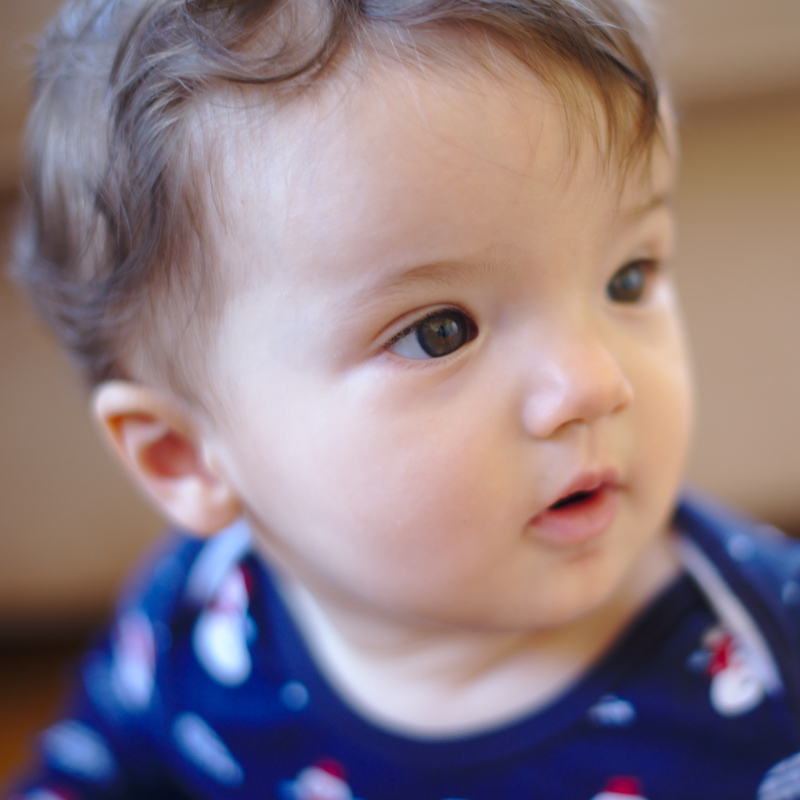
\includegraphics[width=3cm]{figures/theo6.jpg}}\\[1mm]
\hfill
\begin{tikzpicture}
  \begin{scope}
    \clip (0,0) circle[radius=1.5cm];
    \node[circle, thin border] (theo1) at (0,0) {\theo};
  \end{scope}
  \draw[->,opacity=.6] (-1.8,0) -- (1.8,0);
  \draw[->,opacity=.6] (0,-1.8) -- (0,1.8);

  \begin{scope}[xshift=7cm]
  \begin{scope}[rotate=45]
    \clip (0,0) circle[radius=1.5cm];
    \node[transform shape, circle, thin border] 
      (theo2) at (0,0) {\theo};
  \end{scope}
  \draw[->,opacity=.6] (-1.8,0) -- (1.8,0);
  \draw[->,opacity=.6] (0,-1.8) -- (0,1.8);
  \end{scope}

  \draw[->] ($(theo1.east)+(0,.3)$) to[bend left]
    node[midway,above] {$A$}
    node[midway,below=5mm,text width=3cm,align=center] 
      {no nonzero vector $x$ is collinear with $Ax$}
    ($(theo2.north west)+(0,.3)$);

\end{tikzpicture}
\hfill\null

\pause
or algebraically:
\[ f(\lambda) = \lambda^2 - \Tr(A)\,\lambda + \det(A)
= \lambda^2 - \sqrt 2\,\lambda + 1\pause
\implies \lambda = \frac{\sqrt 2\pm\sqrt{-2}}2. \]

\end{frame}


%%%%%%%%%%%%%%%%%%%%%%%%%%%%%%%%%%%%%%%%%%%%%%%%%%%%%%%%%%%%%%%%%%%

\begin{frame}
\frametitle{Complex Numbers}

It makes us sad that $-1$ has no square root.
\pause
If it did, then $\sqrt{-2} = \sqrt{2}\cdot\sqrt{-1}$.

\pause\medskip
\alert{Mathematician's solution:} we're just not using enough numbers!
\pause
We're going to declare by \emph{fiat} that there exists a square root of $-1$.

\pause
\begin{defn}
  The number $i$ is defined such that $i^2 = -1$.
\end{defn}

\pause
Once we have $i$, we have to allow numbers like $a+bi$ for real numbers $a,b$.

\pause
\begin{defn}
  A \emph{complex number} is a number of the form $a+bi$ for $a,b$ in $\R$.
  The set of all complex numbers is denoted $\C$.
\end{defn}

\pause\medskip
Note $\R$ is contained in $\C$: they're the numbers $a + 0i$.

\pause\medskip
We can identify $\C$ with $\R^2$ by $a+bi \ToT {a\choose b}$.
\pause
So when we draw a picture of $\C$, we draw the plane:\\
\hfill
\begin{tikzpicture}[scale=.5, whitebg nodes, thin border nodes]
  \draw[grid lines] (-2,-2) grid (2,2);
  \draw[thick, ->] (-2,0) -- (2,0);
  \draw[<-, overlay] (-2.05,0) -- (-2.5,0) node[left] {real axis};
  \draw[thick, ->] (0,-2) -- (0,2);
  \draw[<-, overlay] (-.05,-1.5) -- ++(-2.5,0) node[left] {imaginary axis};
  \point["$1$" above] at (1,0);
  \point["$i$" left] at (0,1);
  \point at (0,0);
  \point["$1-i$" below] at (1,-1);
\end{tikzpicture}
\hfill\null

\end{frame}


%%%%%%%%%%%%%%%%%%%%%%%%%%%%%%%%%%%%%%%%%%%%%%%%%%%%%%%%%%%%%%%%%%%

\begin{frame}
\frametitle{Why This Is Not A Weird Thing To Do}
\framesubtitle{An anachronistic historical aside}

\small
In the beginning, people only used counting numbers for, well, counting things:
$1,2,3,4,5,\ldots$.
\pause
Then someone (Persian mathematician Mu\underdot{h}ammad ibn M\=us\=a
al-Khw\=arizm\=\i, 825) had the ridiculous idea that there should be a number
$0$ that represents an absence of quantity.
\pause
This blew everyone's mind.

\pause\medskip
Then it occurred to someone (Chinese mathematician Liu Hui, c.\ 3rd century)
that there should be \emph{negative} numbers to represent a deficit in quantity.
\pause
That seemed reasonable, until people realized that $10 + (-3)$ would have to
equal $7$.
\pause
This is when people started saying, ``bah, math is just too hard for me.''

\pause\medskip
At this point it was inconvenient that you couldn't divide $2$ by $3$.
\pause
Thus someone (Indian mathematician Aryabhatta, c.\ 5th century) invented
fractions (rational numbers) to represent fractional quantities.
\pause
These proved very popular.  The Pythagoreans developed a whole belief system
around the notion that any quantity worth considering could be broken down into
whole numbers in this way.

\pause\medskip
Then the Pythagoreans (c.\ 6th century BCE) discovered that the hypotenuse of an
isosceles right triangle with side length $1$ (i.e.\ $\sqrt 2$) is not a
fraction.
\pause
This caused a serious existential crisis and led to at least one death by
drowning.
\pause
The real number $\sqrt 2$ was thus invented to solve the equation $x^2-2=0$.

\pause\medskip
So what's so strange about inventing a number $i$ to solve the equation $x^2+1=0$?

\end{frame}


%%%%%%%%%%%%%%%%%%%%%%%%%%%%%%%%%%%%%%%%%%%%%%%%%%%%%%%%%%%%%%%%%%%

\begin{frame}
\frametitle{Operations on Complex Numbers}

\alert{Addition:}
\webonlycmd{$(2-3i) + (-1+i) = 1 - 2i$.}

\medskip
\alert{Multiplication:}
\webonlycmd{$(2-3i)(-1+i) = 2(-1) + 2i + 3i -3i^2 = -2 + 5i + 3 = 1+5i$.}

\pause\medskip
\alert{Complex conjugation:} 
$\bar{a+bi} = a-bi$ is the \textbf{complex conjugate} of $a+bi$.\\
\pause
\alert{Check:} $\bar{z+w} = \bar z + \bar w$ and $\bar{zw} = \bar z\cdot\bar w$.

\pause\medskip
\alert{Absolute value:}
$|a+bi| = \sqrt{a^2+b^2}$.
\pause
This is a \emph{real} number.\\
\pause
\alert{Note:} $(a+bi)(\bar{a+bi}) = (a+bi)(a-bi) = a^2 - (bi)^2 = a^2+b^2$.
\pause
So $|z| = \sqrt{z\bar z}$.\\
\pause
\alert{Check:}
$|zw| = |z|\cdot|w|$.

\pause\medskip
\alert{Division by a nonzero real number:}
$\displaystyle\frac{a+bi}c = \frac ac + \frac bci$.

\pause\medskip
\alert{Division by a nonzero complex number:}
$\displaystyle\frac zw = \frac{z\bar w}{w\bar w} = \frac{z\bar w}{|w|^2}$.

\pause\medskip
\alert{Example:}
\[ \frac{1+i}{1-i} = \webonlycmd{\frac{(1+i)^2}{1^2+(-1)^2} = \frac{1+2i+i^2}2 = i.} \]

\pause\medskip
\alert{Real and imaginary part:}
$\Re(a+bi) = a \qquad \Im(a+bi) = b$.

\end{frame}


%%%%%%%%%%%%%%%%%%%%%%%%%%%%%%%%%%%%%%%%%%%%%%%%%%%%%%%%%%%%%%%%%%%

\begin{frame}
\frametitle{Polar Coordinates for Complex Numbers}

\begin{minipage}[c]{.6\linewidth}
  Any complex number $z=a+bi$ has the polar coordinates
  \[ z = |z|(\cos\theta + i\sin\theta). \]
  The angle $\theta$ is called the \textbf{argument} of $z$, and is denoted
  $\theta = \arg(z)$.
  \uncover<2->{Note $\arg(\bar z) = -\arg(z)$.}
\end{minipage}\hfill
\begin{tikzpicture}[baseline=1cm, decoration={brace,raise=2pt}]
  \coordinate (z) at (1,2);
  \coordinate (x) at (z |- 0,0);
  \coordinate (o) at (0,0);
  \draw[very thin] (-.2,0) -- (1.4,0);
  \draw[very thin] (0,-.2) -- (0,2.2);
  \draw[vector] (0,0) -- node[anchor=south east,inner sep=.5pt,fill=white]
    {$|z|$} (z) node[above] {$z$};
  \point at (0,0);
  \draw[decorate, decoration=mirror] (0,0) -- node[below=3pt]{$a$} (x);
  \draw[decorate] (z) -- node[right=2pt]{$b$} (x);
  \pic[draw,"$\theta$"] {angle = x--o--z};
\end{tikzpicture}\hfill\null

\pause[3]\medskip
When you multiply complex numbers, you multiply the absolute values and add the
arguments:
\[ |zw| = |z|\,|w| \qquad \arg(zw) = \arg(z)+\arg(w). \]
\begin{center}
\begin{tikzpicture}[thin border nodes=.5pt]
  \coordinate (z) at (1,2);
  \coordinate (w) at (1,1);
  \coordinate (u) at (-1,3);
  \coordinate (o) at (0,0);
  \coordinate (x) at (1,0);
  \draw[very thin] (-1.2,0) -- (2.7,0);
  \draw[very thin] (0,-.2) -- (0,3.2);

  \draw[vector,seq-blue] (o) --
    node[auto] {$|z|$} (z)
    node[above] {$z$};
  \draw[vector,seq-green] (o) --
    node[auto,near end,swap] {$|w|$} (w) 
    node[above] {$w$};
  \pic[draw,->,seq-blue,"$\theta$"] {angle = x--o--z};
  \pic[draw,->,seq-green,"$\phi$",angle radius=.8cm,angle eccentricity=.8]
    {angle = x--o--w};
  \draw[vector,seq-violet] (o) --
    node[auto] {$|z|\,|w|$} (u) 
    node[above] {$zw$};
  \pic[draw,->,seq-violet,"$\theta+\phi$",angle radius=2.5cm,angle eccentricity=1.15]
    {angle = x--o--u};
  
  \point at (0,0);
\end{tikzpicture}
\end{center}

\end{frame}


%%%%%%%%%%%%%%%%%%%%%%%%%%%%%%%%%%%%%%%%%%%%%%%%%%%%%%%%%%%%%%%%%%%

\begin{frame}
\frametitle{The Fundamental Theorem of Algebra}

The whole point of using complex numbers is to solve polynomial equations.  It
turns out that they are enough to find all solutions of all polynomial equations:

\pause
\begin{oneoffthm}{Fundamental Theorem of Algebra}
  Every polynomial of degree $n$ has exactly $n$ complex roots, counted with
  multiplicity.
\end{oneoffthm}

\pause\medskip
Equivalently, if $f(x) = x^n + a_{n-1}x^{n-1}+\cdots+a_1 x+a_0$ is a polynomial
of degree $n$, then
\[ f(x) = (x-\lambda_1)(x-\lambda_2)\cdots(x-\lambda_n) \]
for (not necessarily distinct) complex numbers
$\lambda_1,\lambda_2,\ldots,\lambda_n$. 

\pause\medskip
\begin{bluebox}[Important]{.9\linewidth}
  If $f$ is a polynomial with \emph{real} coefficients, and if $\lambda$ is a
  root of $f$, then so is $\bar\lambda$:
  \[\begin{split} 0 = \bar{f(\lambda)}
    &= \bar{\lambda^n + a_{n-1}\lambda^{n-1}+\cdots+a_1\lambda+a_0} \\
    &= \bar\lambda{}^n + a_{n-1}\bar\lambda{}^{n-1}+\cdots+a_1\bar\lambda+a_0 
    = f\bigl(\bar\lambda\bigr). \end{split}\]
  \pause
  Therefore complex roots of real polynomials come in \emph{conjugate pairs}.

\end{bluebox}

\end{frame}


%%%%%%%%%%%%%%%%%%%%%%%%%%%%%%%%%%%%%%%%%%%%%%%%%%%%%%%%%%%%%%%%%%%

\begin{frame}
\frametitle{The Fundamental Theorem of Algebra}
\framesubtitle{Examples}

\alert{Degree $2$:}
The quadratic formula gives you the (real or complex) roots of any degree-$2$
polynomial:
\[ f(x) = x^2+bx+c \implies x = \frac{-b\pm\sqrt{b^2-4c}}2. \]
\pause
For instance, if $f(\lambda) = \lambda^2 - \sqrt 2\lambda + 1$ then
\[ \lambda = \webonlycmd{\frac{\sqrt 2\pm\sqrt{-2}}2 = \frac{\sqrt 2}2(1\pm i)
  = \frac {1\pm i}{\sqrt 2}.} \]
\pause
Note the roots are complex conjugates if $b,c$ are real.

\end{frame}


%%%%%%%%%%%%%%%%%%%%%%%%%%%%%%%%%%%%%%%%%%%%%%%%%%%%%%%%%%%%%%%%%%%

\begin{frame}
\frametitle{The Fundamental Theorem of Algebra}
\framesubtitle{Examples}

\alert{Degree $3$:}
A real cubic polynomial has either
\pause
three real roots, or
\pause
one real root and a conjugate pair of complex roots.
\pause
The graph looks like:
\begin{center}
\begin{tikzpicture}[domain=-2:2,smooth,scale=.3,baseline]
  \draw (-2,0) -- (2,0);
  \draw[color=seq-red, <->] plot (\x,\x^3-2*\x+.5);
\end{tikzpicture}
\quad or \quad
\begin{tikzpicture}[domain=-2:2,smooth,scale=.3,yscale=.7,baseline]
  \draw (-2,0) -- (2,0);
  \draw[color=seq-red, <->] plot (\x,\x^3-\x+.7);
\end{tikzpicture}
\end{center}
respectively.

\pause\medskip
\alert{Example:} let
$f(\lambda) = 5\lambda^3 - 18\lambda^2 + 21\lambda - 10$.\\[1mm]
\begin{webonly}
Since $f(2) = 0$, we can do polynomial long division by $\lambda-2$: we get
$f(\lambda) = (\lambda-2)\left( 5\lambda^2-8\lambda+5 \right)$.
Using the quadratic formula, the second polynomial has a root when
\[ \lambda = \frac{8 \pm \sqrt{64-100}}{10}
= \frac 45 \pm \frac{\sqrt{-36}}{10}
= \frac{4 \pm 3i}5. \]
Therefore,
\[ f(\lambda) = 5(\lambda-2)\left( \lambda-\frac{4+3i}5 \right)
\left( \lambda-\frac{4-3i}5 \right). \]
\end{webonly}

\end{frame}


%%%%%%%%%%%%%%%%%%%%%%%%%%%%%%%%%%%%%%%%%%%%%%%%%%%%%%%%%%%%%%%%%%%

\begin{pollframe}

\bigskip
The characteristic polynomial of 
\[ A = \frac 1{\sqrt 2}\mat{1 -1; 1 1} \]
is $f(\lambda) = \lambda^2-\sqrt 2\lambda+1$.  This has two complex roots
$(1\pm i)/\sqrt 2$.

\begin{poll}
\pause\bigskip
\begin{bluebox}[Poll]{.8\linewidth}
  Does $A$ have any eigen\emph{vectors}?  If so, what are they?
\end{bluebox}
\end{poll}

\end{pollframe}


%%%%%%%%%%%%%%%%%%%%%%%%%%%%%%%%%%%%%%%%%%%%%%%%%%%%%%%%%%%%%%%%%%%

\begin{frame}
\frametitle{A Matrix \emph{with} an Eigenvector}

\emph{Every} matrix is guaranteed to have \emph{complex} eigenvalues and
eigenvectors.
\pause
Using rotation by $\pi/4$ from before:
\abovedisplayskip=5pt\belowdisplayskip=\abovedisplayskip
\[ A = \frac 1{\sqrt 2}\mat{1 -1; 1 1}
\sptxt{has eigenvalues} \lambda=\frac{1\pm i}{\sqrt 2}. \]
\pause
Let's compute an eigenvector for $\lambda=(1+i)/\sqrt 2$:
\begin{webonly}
\[ A-\lambda I = \frac 1{\sqrt 2}\mat{1-(1+i) -1; 1 1-(1+i)} =
\frac 1{\sqrt 2}\mat{-i -1; 1 -i}. \]
The second row is $i$ times the first, so we row reduce:
\[ \frac 1{\sqrt 2}\mat{-i -1; 1 -i} \;\longsquiggly\;
\frac 1{\sqrt 2}\mat{-i -1; 0 0} \;\longsquiggly[divide by $-i/\sqrt2$]\;
\mat{1 -i; 0 0}. \]
The parametric form is $x = iy$, so an eigenvector is $\vec{i 1}$.
\end{webonly}

\pause
A similar computation shows that an eigenvector for $\lambda=(1-i)/\sqrt 2$ is 
$\vec{-i 1}$.
\pause
So is $i\vec{-i 1} = \vec{1 i}$ (you can scale by \emph{complex} numbers).

\end{frame}


%%%%%%%%%%%%%%%%%%%%%%%%%%%%%%%%%%%%%%%%%%%%%%%%%%%%%%%%%%%%%%%%%%%

\begin{frame}
\frametitle{A Trick for Computing Eigenvectors of $2\times 2$ Matrices}
\framesubtitle{Very useful for complex eigenvalues}

Let $A$ be a $2\times 2$ matrix, and let $\lambda$ be an eigenvalue of $A$.

\pause\medskip
Then $A-\lambda I$ is not invertible, so the second row is \emph{automatically}
a multiple of the first.
\pause
(Think about it for a while: otherwise the rref is 
$\begin{psmm}1&0\\0&1\end{psmm}$.)

\pause\medskip
Hence the second row disappears in the rref, so \emph{we don't care what it is!}

\pause\medskip
If $A - \lambda I = \mat{a b; \star, \star}$, then $(A-\lambda I)\vec{b -a} =
0$, so $\vec{b -a}$ is an eigenvector.  
\pause
So is $\vec{-b a}$.

\pause\medskip
\alert{Example:}
\[ \displaystyle A = \frac 1{\sqrt 2}\mat{1 -1; 1 1} \qquad
\lambda = \frac{1-i}{\sqrt 2}. \]
\begin{webonly}%
  Then:
  \[ A-\lambda I = \frac 1{\sqrt 2}\mat{i -1; \star, \star} \]
  so an eigenvector is 
  \[ v = \vec{1 i}. \]
\end{webonly}

\end{frame}


%%%%%%%%%%%%%%%%%%%%%%%%%%%%%%%%%%%%%%%%%%%%%%%%%%%%%%%%%%%%%%%%%%%

\begin{frame}
\frametitle{Conjugate Eigenvectors}

For $\displaystyle A = \frac 1{\sqrt 2}\mat{1 -1; 1 1}$,
\[\begin{split}
  \text{the eigenvalue $\frac{1+i}{\sqrt 2}$} & \text{ has eigenvector} \vec{i 1}.\\
  \text{the eigenvalue $\frac{1-i}{\sqrt 2}$} & \text{ has eigenvector} \vec{-i 1}.\\
\end{split}\]
\pause
Do you notice a pattern?
\pause

\begin{fact2}
  Let $A$ be a real square matrix.  If $\lambda$ is an eigenvalue with
  eigenvector $v$, then $\bar\lambda$ is an eigenvalue with eigenvector $\bar v$.
\end{fact2}

\pause\medskip
\alert{Why?}
\[ Av = \lambda \implies A\bar v = \bar{Av} = \bar{\lambda v}
= \bar\lambda\bar v. \]

\pause\smallskip
\begin{bluebox}{.6\linewidth}
  Both eigenvalues and eigenvectors of real square matrices occur in conjugate pairs.
\end{bluebox}

\end{frame}


%%%%%%%%%%%%%%%%%%%%%%%%%%%%%%%%%%%%%%%%%%%%%%%%%%%%%%%%%%%%%%%%%%%

\begin{frame}
\frametitle{A $3\times 3$ Example}

Find the eigenvalues and eigenvectors of
\[ A = \mat{\frac 45 -\frac 35 0; \frac 35 \frac 45 0; 0 0 2}. \]
\pause
The characteristic polynomial is
\webonlycmd{
\[ f(\lambda) = \det\mat{\frac 45-\lambda, -\frac 35 0; \frac 35 \frac 45-\lambda, 0;
  0 0 2-\lambda}
= \namedbox{factor}{(2-\lambda)}\left( \lambda^2 - \frac 85\lambda + 1 \right). \]
\begin{tikzpicture}[remember picture, overlay]
  \node[blue!50, rounded corners, draw, fit=(factor), inner sep=2pt] (factorbox) {};
  \path (factorbox.north) ++(8mm,11mm)
    node[blue!50, align=center, text width=3cm, right, inner sep=0pt] (expl)
      {This factors out automatically if you expand cofactors along the third
        row or column};
  \draw[->, blue!50, shorten >=1pt] (expl.west) to[out=180, in=90] (factorbox.north);
\end{tikzpicture}}
\pause
We computed the roots of this polynomial (times $5$) before:
\[ \lambda =\quad 2,\quad \frac{4+3i}5,\quad \frac{4-3i}5. \]
\pause
We eyeball an eigenvector with eigenvalue $2$ as $(0,0,1)$.

\end{frame}


%%%%%%%%%%%%%%%%%%%%%%%%%%%%%%%%%%%%%%%%%%%%%%%%%%%%%%%%%%%%%%%%%%%

\begin{frame}
\frametitle{A $3\times 3$ Example}
\framesubtitle{Continued}

\vskip -5mm
\[ A = \mat{\frac 45 -\frac 35 0; \frac 35 \frac 45 0; 0 0 2} \]
To find the other eigenvectors, we row reduce:
\begin{webonly}
\[ A-\frac{4+3i}5I = 
\mat{-\frac 35i -\frac 35 0; \frac 35 -\frac 35i, 0;
  0 0 2-\frac{4+3i}5}
\;\longsquiggly[scale rows]\;
\mat{-i -1 0; 1 -i 0; 0 0 1}\]
The second row is $i$ times the first:
\[ \longsquiggly[row replacement]\;
\mat{-i -1 0; 0 0 0; 0 0 1}
\;\longsquiggly[divide by $-i$,swap]\;
\mat{1 -i 0; 0 0 1; 0 0 0}.
\]
The parametric form is $x=iy,\,z=0$, so an eigenvector is
$\vec{i 1 0}$.
Therefore, an eigenvector with conjugate eigenvalue $\displaystyle\frac{4-3i}5$ is 
$\vec{-i 1 0}$.
  
\end{webonly}

\end{frame}


%%%%%%%%%%%%%%%%%%%%%%%%%%%%%%%%%%%%%%%%%%%%%%%%%%%%%%%%%%%%%%%%%%%

\begin{frame}
\frametitle{Geometric Interpretation of Complex Eigenvectors}
\framesubtitle{$2\times 2$ case}

\vskip-3mm
\abovedisplayskip=5pt\belowdisplayskip=\abovedisplayskip
\begin{thm}
  Let $A$ be a $2\times 2$ matrix with complex (non-real) eigenvalue $\lambda$,
  and let  $v$ be an eigenvector.  Then
  \[ A = PCP\inv \]
  where
  \[ P = \mat{| |; \Re v \Im v; | |}
  \sptxt{and}
  C = \mat{\Re\lambda, \Im\lambda; -\Im\lambda, \Re\lambda}. \]
  \pause
  The matrix $C$ is a composition of rotation by $-\arg(\lambda)$ and scaling by
  $|\lambda|$:
  \[ C = \mat{|\lambda| 0; 0 |\lambda|}
    \mat{
      \cos(-\arg(\lambda)) -\sin(-\arg(\lambda));
      \sin(-\arg(\lambda)) \cos(-\arg(\lambda))
    }. \]
\end{thm}

\pause
\begin{bluebox}{.9\linewidth}
  A $2\times 2$ matrix with complex eigenvalue $\lambda$ is similar to (rotation
  by the argument of $\bar\lambda$) composed with (scaling by $|\lambda|$).
  This is multiplication by $\bar\lambda$ in $\C\sim\R^2$.
\end{bluebox}

\end{frame}


%%%%%%%%%%%%%%%%%%%%%%%%%%%%%%%%%%%%%%%%%%%%%%%%%%%%%%%%%%%%%%%%%%%

\begin{frame}
\frametitle{Geometric Interpretation of Complex Eigenvalues}
\framesubtitle{$2\times 2$ example}

What does $\displaystyle A = \mat{1 -1; 1 1}$ do geometrically?

\begin{webonly}
\begin{itemize}
\item The characteristic polynomial is
  \[ f(\lambda) = \lambda^2 - \Tr(A)\,\lambda + \det(A) 
  = \lambda^2 - 2\lambda + 2. \]
  The roots are
  \[ \frac{2\pm\sqrt{4-8}}2 = 1\pm i. \]
\item Let $\lambda = 1-i$.  We compute an eigenvector $v$:
  \[ A - \lambda I = \mat{i -1; \star, \star}
  \;\longsquiggly\; v = \vec{1 i}. \]
\item Therefore, $A=PCP\inv$ where
  \[\begin{aligned}
    \hss P &= \mat{\Re\vec{1 i} \Im\vec{1 i}} = \mat{1 0; 0 1} \\
     C &= \mat{\Re\lambda, \Im\lambda; -\Im\lambda, \Re\lambda}
       = \mat{1 -1; 1 1 } \hss 
     \end{aligned}\]
\end{itemize}
\end{webonly}
\end{frame}


%%%%%%%%%%%%%%%%%%%%%%%%%%%%%%%%%%%%%%%%%%%%%%%%%%%%%%%%%%%%%%%%%%%

\begin{frame}
\frametitle{Geometric Interpretation of Complex Eigenvalues}
\framesubtitle{$2\times 2$ example, continued}

\vskip-5mm
\[ A = C = \mat{1 -1; 1 1} \qquad \lambda = 1-i \]

\begin{webonly}
\begin{itemize}
\item The matrix $C = A$ scales by a factor of
  \[ |\lambda| = \sqrt{1^2 + 1^2} = \sqrt 2. \]
\item The argument of $\lambda$ is $-\pi/4$:\\[.5mm]
  \hfill\begin{tikzpicture}[yscale=-1]
    \coordinate (z) at (1,1);
    \coordinate (x) at (1,0);
    \coordinate (o) at (0,0);
    \point at (0,0);
    \draw[very thin] (-.1,0) -- (1.1,0);
    \draw[very thin] (0,-.1) -- (0,1.1);
    \draw[vector] (o) to (z) node[right] {$\lambda$};
    \pic[draw, "$\frac\pi4$" font=\scriptsize, angle radius=.75cm]
      {angle = z--o--x};
    \end{tikzpicture}\hfill\null\\
  Therefore $C = A$ rotates by $+\pi/4$.
\item (We already knew this because $A = \sqrt 2$ times the matrix for rotation
  by $\pi/4$ from before.)
\end{itemize}
\end{webonly}

\pause
\def\theo{
\includegraphics[width=2.828427cm]{figures/theo5.jpg}}
\hfill\begin{tikzpicture}
  \begin{scope}
    \clip (0,0) circle[radius=1];
    \node[circle, scale=1/sqrt(2)] (theo1) at (0,0) {\theo};
  \end{scope}

  \begin{scope}[opacity=.6, black!15]
    \draw[->] (-1.3,0) -- (1.3,0) node[coordinate] (l) {};
    \draw[->] (0,-1.3) -- (0,1.3);
  \end{scope}
  \draw[->,red] (1.1,0) arc[radius=1.1,start angle=0,delta angle=30];

  \begin{scope}[xshift=7cm]
    \begin{scope}
      \clip (0,0) circle[radius=sqrt(2)];
      \node[circle, rotate=30] (theo2) at (0,0) {\theo};
    \end{scope}

    \begin{scope}[opacity=.6, black!15]
      \draw[->] (-1.3,0) node[coordinate] (r) {} -- (1.3,0);
      \draw[->] (0,-1.3) -- (0,1.3);
    \end{scope}
  \end{scope}

  \draw[->] ($(l)+(3mm,3mm)$) to[bend left]
    node[midway,above] {$A$}
    node[midway,below=.5cm,align=center] 
      {rotate by $\pi/4$\\scale by $\sqrt 2$}
    ($(r)+(-3mm,3mm)$);

\end{tikzpicture}
\hfill\null\\

\end{frame}


%%%%%%%%%%%%%%%%%%%%%%%%%%%%%%%%%%%%%%%%%%%%%%%%%%%%%%%%%%%%%%%%%%%

\begin{frame}
\frametitle{Geometric Interpretation of Complex Eigenvalues}
\framesubtitle{Another $2\times 2$ example}

What does
$\displaystyle A = \mat{\sqrt 3+1 -2; 1 \sqrt 3-1}$ do geometrically?

\medskip
\begin{webonly}
\begin{itemize}
\item The characteristic polynomial is
  \[ f(\lambda) = \lambda^2 - \Tr(A)\,\lambda + \det(A) 
  = \lambda^2 - 2\sqrt 3\,\lambda + 4. \]
  The roots are
  \[ \frac{2\sqrt 3\pm\sqrt{12-16}}2 = \sqrt 3\pm i. \]
\item Let $\lambda = \sqrt 3-i$.  We compute an eigenvector $v$:
  \[ A-\lambda I = \mat{1+i -2; \star, \star} \;\longsquiggly\;
  v = \vec{1-i 1}. \]
\item It follows that $A = PCP\inv$ where
  \[\begin{aligned} 
    P &= \mat{\Re\vec{1-i 1} \Im\vec{1-i 1}} = \mat{1 -1; 1 0} \\
    C &= \mat{\Re\lambda, \Im\lambda; -\Im\lambda, \Re\lambda} 
    = \mat{\sqrt 3 -1; 1 \sqrt 3}. 
  \end{aligned}\]

\end{itemize}
\end{webonly}

\end{frame}


%%%%%%%%%%%%%%%%%%%%%%%%%%%%%%%%%%%%%%%%%%%%%%%%%%%%%%%%%%%%%%%%%%%

\begin{frame}
\frametitle{Geometric Interpretation of Complex Eigenvalues}
\framesubtitle{Another $2\times 2$ example, continued}

\vskip-5mm
\[ A = \mat{\sqrt 3+1 -2; 1 \sqrt 3-1} \qquad
C = \mat{\sqrt 3 -1; 1 \sqrt 3} \qquad
\lambda = \sqrt 3-i \]

\begin{webonly}
\begin{itemize}
\item The matrix $C$ scales by a factor of
  \[ |\lambda| = \sqrt{(\sqrt 3)^2 + (-1)^2} = \sqrt 4 = 2. \]
\item The argument of $\lambda$ is $-\pi/6$:\\[.5mm]
  \hfill\begin{tikzpicture}[scale=1.2, thin border nodes]
    \coordinate (z) at ({sqrt(3)/2},-1/2);
    \coordinate (x) at (1,0);
    \coordinate (o) at (0,0);
    \point at (0,0);
    \draw[very thin] (-.1,0) -- (1.1,0);
    \draw[very thin] (0,-.6) -- (0,.1);
    \draw[vector] (o) to["$\lambda$"'] (z);
    \pic[draw, "$\frac\pi6$" font=\scriptsize, 
        angle radius=.75cm, angle eccentricity=.85]
      {angle = z--o--x};
    \draw[decoration={brace,raise=1pt}, decorate] 
      ({sqrt(3)/2},0) to["$1$" xshift=3pt] (z);
    \draw[decoration={brace,raise=1pt,mirror}, decorate] 
      (0,-1/2) to["$\sqrt 3$"' yshift=-3pt] (z);
  \end{tikzpicture}\hfill\null\\
  Therefore $C$ rotates by $+\pi/6$.

\end{itemize}
\end{webonly}

\end{frame}


%%%%%%%%%%%%%%%%%%%%%%%%%%%%%%%%%%%%%%%%%%%%%%%%%%%%%%%%%%%%%%%%%%%

\begin{frame}
\frametitle{Geometric Interpretation of Complex Eigenvalues}
\framesubtitle{Another $2\times 2$ example: picture}

What does
$\displaystyle A = \mat{\sqrt 3+1 -2; 1 \sqrt 3-1}$ do geometrically?

\def\theo{
\includegraphics[width=2.828427cm]{figures/theo5.jpg}}
\hfill
\begin{tikzpicture}
  \useasboundingbox (3.5,{sqrt(2)}) -- (3.5,{-sqrt(2)});
  \begin{scope}
    \clip (0,0) circle[radius=1/sqrt(2)];
    \node[circle,scale=1/2] (theo1) at (0,0) {\theo};
  \end{scope}

  \begin{scope}[opacity=.6, black!15]
    \draw[->] (-1.3,0) -- (1.3,0) node[coordinate] (l) {};
    \draw[->] (0,-1.3) -- (0,1.3);
    \draw (0,0) circle[radius=1];
  \end{scope}
  \draw[->,red] (1.1,0) arc[radius=1.1,start angle=0,delta angle=30];

  \begin{scope}[xshift=7cm]
    \begin{scope}
      \clip (0,0) circle[radius=sqrt(2)];
      \node[circle, rotate=30] (theo2) at (0,0) {\theo};
    \end{scope}

    \begin{scope}[opacity=.6, black!15]
      \draw[->] (-1.3,0) node[coordinate] (r) {} -- (1.3,0);
      \draw[->] (0,-1.3) -- (0,1.3);
      \draw (0,0) circle[radius=1];
    \end{scope}
  \end{scope}

  \draw[->] ($(l)+(3mm,3mm)$) to[bend left]
    node[midway,above] {$C$}
    node[midway,below=.5cm,align=center] {rotate by $\pi/6$\\scale by $2$}
    ($(r)+(-3mm,3mm)$);

\end{tikzpicture}
\hfill\null\\
\pause
$A = PCP\inv$ does the same thing, but with respect to the basis
$\cB = \bigl\{ {1\choose 1},\,{-1\choose 0} \bigr\}$ of columns of $P$:\\
\def\theo{
\includegraphics[width=4cm]{figures/theo5.jpg}}
\hfill
\begin{tikzpicture}
  \useasboundingbox (3.5,{sqrt(2)}) -- (3.5,{-sqrt(2)});
  \begin{scope}
    \clip[cm={1,1,-1,0,(0,0)}] (0,0) ellipse[radius=1/sqrt(2)];
    \node[scale=1/2] (theo1) at (0,0) {\theo};
  \end{scope}

  \begin{scope}[opacity=.6, black!15]
    \draw[->] (-1.3,0) -- (1.3,0) node[coordinate] (l) {};
    \draw[->] (0,-1.3) -- (0,1.3);
  \end{scope}

  \begin{scope}[cm={1,1,-1,0,(0,0)}]
    \draw[opacity=.6, black!15] (0,0) circle[radius=1];
    \draw[->,red] (1.1,0) arc[radius=1.1,start angle=0,delta angle=30];
  \end{scope}
  \draw[vector] (0,0) -- (1,1);
  \draw[vector] (0,0) -- (-1,0);

  \begin{scope}[xshift=7cm]
    \begin{scope}[cm={(sqrt(3)+1)/2,1/2,-1,(sqrt(3)-1)/2,(0,0)}]
      \clip[cm={1,1,-1,0,(0,0)}] (0,0) ellipse[radius=sqrt(2)];
      \node[transform shape] (theo2) at (0,0) {\theo};
    \end{scope}
    \begin{scope}[opacity=.6, black!15]
      \draw[->] (-1.3,0) node[coordinate] (r) {} -- (1.3,0);
      \draw[->] (0,-1.3) -- (0,1.3);
      \draw[cm={1,1,-1,0,(0,0)}] (0,0) ellipse[radius=1];
    \end{scope}
  \end{scope}

  \draw[->] ($(l) + (3mm,3mm)$) to[bend left]
    node[midway,above] {$A$}
    node[midway,below=.5cm,align=center] 
      {``rotate around an ellipse''\\
      scale by $2$}
    ($(r) + (-3mm,3mm)$);

\end{tikzpicture}
\hfill\null

\end{frame}


%%%%%%%%%%%%%%%%%%%%%%%%%%%%%%%%%%%%%%%%%%%%%%%%%%%%%%%%%%%%%%%%%%%

\begin{frame}
\frametitle{Classification of $2\times 2$ Matrices with a Complex Eigenvalue}
\framesubtitle{Triptych}

Let $A$ be a real matrix with a complex eigenvalue $\lambda$.
\pause
One way to understand the geometry of $A$ is to consider the difference equation
$v_{n+1} = Av_n$, i.e.\ the sequence of vectors $v,Av,A^2v,\ldots$
\pause
\pgfmathsetmacro{\sqrtii}{sqrt(2)}
\hbox to \linewidth{\hss
\parbox{4.1cm}{\centering
\vbox{\small
\[\begin{aligned}
  A =  \frac 1{\sqrt 2}&\mat{\sqrt 3+1 -2; 1 \sqrt 3-1}\\
  \lambda &= \frac{\sqrt 3-i}{\sqrt 2}\\
  \color{seq-red}|\lambda| &\color{seq-red}> 1
\end{aligned} \]\vss}
\begin{tikzpicture}[scale=.4, samples at={0,.25,...,4.25}, 
    smooth, tension=.5, thin border nodes=2pt]
  \useasboundingbox (-4,-4) rectangle (4,4);
  \draw[dashed, cm={1,1,-1,0,(0,0)}] (0,0) ellipse[radius=10/4];
  \draw[->, very thin] (-4,0) -- (4,0);
  \draw[->, very thin] (0,-4) -- (0,4);
  \begin{scope}[cm={1,1,-1,0,(0,0)}, <->/.tip={Stealth}]
  \foreach \rot in {0,60,...,359} {
    \draw[seq-blue,rotate=\rot]
      plot ({\sqrtii^\x*cos(\x*30)},{\sqrtii^\x*sin(\x*30)});
    % Can't use decorations.markings for this; it exceeds TeX's limited
    % capacity for numerical calculations.
    \foreach \x in {0,3,4.25} {
      \draw[seq-blue,->,rotate=\rot] 
        ({\sqrtii^\x*cos(\x*30)},{\sqrtii^\x*sin(\x*30)}) --
        ({\sqrtii^(\x+.1)*cos((\x+.1)*30)},{\sqrtii^(\x+.1)*sin((\x+.1)*30)});
    }
  }
  \foreach \x in {0,1,2,3} {
    \pgfmathsetmacro{\y}{\x+1.1}
    \coordinate (v\x) at ({\sqrtii^\y*cos(\y*30+180)},{\sqrtii^\y*sin(\y*30+180)});
    \draw[vector,seq-green] (0,0) -- (v\x)
      node[point,seq-green,scale=.5] {};
  }
  \end{scope}
  \foreach \x in {0,1,2,3} {
    \pgfmathanglebetweenpoints{\pgfpoint{0cm}{0cm}}{\pgfpointanchor{v\x}{center}}
    \node[anchor={\pgfmathresult+180},seq-green] at (v\x)
      {$\ifnum\x>0\ifnum\x>1A^\x\else A\fi\fi v$};
  }
  \point at (0,0);
\end{tikzpicture}
``spirals out''}
%
\pause\hfill
\parbox{4.1cm}{\centering
\vbox{\small
\[\begin{aligned}
  A =  \frac 12&\mat{\sqrt 3+1 -2; 1 \sqrt 3-1}\\
  \lambda &= \frac{\sqrt 3-i}2\\
  \color{seq-red}|\lambda| &\color{seq-red}= 1
\end{aligned} \]\vss}
\begin{tikzpicture}[scale=.1, thin border nodes=2pt,
    decoration={markings, mark=between positions 0 and .75 step .25
      with {\arrow{Stealth}}}]
  \useasboundingbox (-16,-16) rectangle (16,16);
  \draw[->, very thin] (-16,0) -- (16,0);
  \draw[->, very thin] (0,-16) -- (0,16);
  \draw[postaction=decorate, seq-blue, cm={1,1,-1,0,(0,0)}]
    (0,0) ellipse[radius=10];
  \foreach \x in {0,...,3} {
    \pgfmathsetmacro{\y}{\x-.4}
    \begin{scope}[cm={1,1,-1,0,(0,0)}]
    \coordinate (v\x) at ({10*cos(\y*30)},{10*sin(\y*30)});
    \draw[vector,seq-green]
      (0,0) -- (v\x)
        node[point,seq-green,scale=.5] {};
    \end{scope}
    \pgfmathanglebetweenpoints{\pgfpoint{0cm}{0cm}}{\pgfpointanchor{v\x}{center}}
    \node[anchor={\pgfmathresult+180},seq-green] at (v\x)
      {$\ifnum\x>0\ifnum\x>1A^\x\else A\fi\fi v$};
  }
  \point at (0,0);
\end{tikzpicture}
``rotates around an ellipse''}
%
\pause\hfill
\parbox{4.1cm}{\centering
\vbox{\small
  \[\begin{aligned}
  A =  \frac 1{2\sqrt2}&\mat{\sqrt 3+1 -2; 1 \sqrt 3-1}\\
  \lambda &= \frac{\sqrt 3-i}{2\sqrt2}\\
  \color{seq-red}|\lambda| &\color{seq-red}< 1
\end{aligned}\]\vss}
\begin{tikzpicture}[scale=.4, samples at={0,.25,...,4.25}, 
    smooth, tension=.5, thin border nodes=2pt]
  \useasboundingbox (-4,-4) rectangle (4,4);
  \draw[dashed, cm={1,1,-1,0,(0,0)}] (0,0) ellipse[radius=10/4];
  \draw[->, very thin] (-4,0) -- (4,0);
  \draw[->, very thin] (0,-4) -- (0,4);
  \begin{scope}[cm={1,1,-1,0,(0,0)}, <->/.tip={Stealth}]
  \foreach \rot in {0,60,...,359} {
    \draw[seq-blue,rotate=\rot]
      plot ({-\sqrtii^\x*cos(\x*30)},{\sqrtii^\x*sin(\x*30)});
    % Can't use decorations.markings for this; it exceeds TeX's limited
    % capacity for numerical calculations.
    \foreach \x in {0,3,4.25} {
      \draw[seq-blue,<-,rotate=\rot] 
        ({-\sqrtii^\x*cos(\x*30)},{\sqrtii^\x*sin(\x*30)}) --
        ({-\sqrtii^(\x+.1)*cos((\x+.1)*30)},{\sqrtii^(\x+.1)*sin((\x+.1)*30)});
    }
  }
  \foreach \x in {3,2,1,0} {
    \pgfmathsetmacro{\y}{(3-\x)+1.1}
    \coordinate (v\x) at (-{\sqrtii^\y*cos(\y*30-120)},{\sqrtii^\y*sin(\y*30-120)});
    \draw[vector,seq-green] (0,0) -- (v\x)
      node[point,seq-green,scale=.5] {};
  }
  \end{scope}
  \foreach \x in {3,2,1,0} {
    \pgfmathanglebetweenpoints{\pgfpoint{0cm}{0cm}}{\pgfpointanchor{v\x}{center}}
    \node[anchor={\pgfmathresult+180},seq-green] at (v\x)
      {$\ifnum\x>0\ifnum\x>1A^\x\else A\fi\fi v$};
  }
  \point at (0,0);
\end{tikzpicture}
``spirals in''}
\hss}

\end{frame}


%%%%%%%%%%%%%%%%%%%%%%%%%%%%%%%%%%%%%%%%%%%%%%%%%%%%%%%%%%%%%%%%%%%

\begin{frame}
\frametitle{Complex Versus Two Real Eigenvalues}
\framesubtitle{An analogy}

\vskip -3mm
\abovedisplayskip=5pt\belowdisplayskip=\abovedisplayskip
\begin{thm}
  Let $A$ be a $2\times 2$ matrix with complex eigenvalue $\lambda = a+bi$
  (where $b\neq 0$), and let $v$ be an eigenvector.  Then
  \[ A = PCP\inv \]
  where
  \[ P = \mat{| |; \Re v \Im v; | |}
  \sptxt{and}
  C = \text{(rotation)}\cdot\text{(scaling)}. \]
\end{thm}

\pause
This is very analogous to diagonalization.  In the $2\times 2$ case:

\pause
\begin{thm}
  Let $A$ be a $2\times 2$ matrix with linearly independent eigenvectors
  $v_1,v_2$ and associated eigenvalues $\lambda_1,\lambda_2$.  Then
  \[ A = PDP\inv \]
  where
  \[ P = \mat{| |; v_1 v_2; | |}
  \sptxt{and}
  D = \mat{\lambda_1 0; 0 \lambda_2}\namedbox{blah}{}. \]
  \pause
  \begin{tikzpicture}[remember picture, overlay]
    \path (blah) ++(1,1) node[blue!50, align=center] (expl)
      {scale $x$-axis by $\lambda_1$\\scale $y$-axis by $\lambda_2$};
    \draw[->, blue!50] (expl.south) to[out=-90,in=0] (blah);
  \end{tikzpicture}
  
\end{thm}

\end{frame}


%%%%%%%%%%%%%%%%%%%%%%%%%%%%%%%%%%%%%%%%%%%%%%%%%%%%%%%%%%%%%%%%%%%

\begin{frame}
\frametitle{Picture with $2$ Real Eigenvalues}

We can draw analogous pictures for a matrix with $2$ real eigenvalues.

\pause\medskip\displayskips{3pt}
\alert{Example:} Let $\displaystyle A = \frac 14\mat{5 3; 3 5}$.
\pause\\
This has eigenvalues $\lambda_1 = 2$ and $\lambda_2 = \frac 12$, with
eigenvectors
\[ v_1 = \vec{1 1} \sptxt{and} v_2 = \vec{-1 1}. \]
\pause
Therefore, $A = PDP\inv$ with
\[ P = \mat{1 -1; 1 1} \sptxt{and} D = \mat{2 0; 0 \frac 12}. \]
\pause
So $A$ scales the $v_1$-direction by $2$ and the $v_2$-direction by $\frac 12$.\\[1mm]
\def\theo{
\includegraphics[width=2cm]{figures/theo5.jpg}}
\hfill
\begin{tikzpicture}[thin border nodes]
  \useasboundingbox (3.5,{sqrt(2)}) -- (3.5,{-sqrt(2)});
  \node (theo1) at (0,0) {\theo};

  \begin{scope}[opacity=.6]
    \draw[->] (-1.3,0) -- (1.3,0) node[coordinate] (l) {};
    \draw[->] (0,-1.3) -- (0,1.3);
  \end{scope}
  \draw[vector] (0,0) -- (1,1) node[above right] {$v_1$};
  \draw[vector] (0,0) -- (-1,1) node[above left] {$v_2$};

  \begin{scope}[xshift=7cm]
    \node[cm={5/4,3/4,3/4,5/4,(0,0)}]
      (theo2) at (0,0) {\theo};
    \begin{scope}[opacity=.6]
      \draw[->] (-1.3,0) node[coordinate] (r) {} -- (1.3,0);
      \draw[->] (0,-1.3) -- (0,1.3);
    \end{scope}
  \draw[vector] (0,0) -- (1,1) node[above right] {$v_1$};
  \draw[vector] (0,0) -- (-1,1) node[above left] {$v_2$};
  \end{scope}

  \draw[->] ($(l)+(0,3mm)$) to[bend left]
    node[midway,above=2pt] {$A$}
    node[midway,below=.5cm,text width=3cm,align=center] 
      {scale $v_1$ by $2$\\scale $v_2$ by $\frac 12$}
    ($(r)+(0,3mm)$);

\end{tikzpicture}
\hfill\null

\end{frame}


%%%%%%%%%%%%%%%%%%%%%%%%%%%%%%%%%%%%%%%%%%%%%%%%%%%%%%%%%%%%%%%%%%%

\begin{frame}
\frametitle{Picture with $2$ Real Eigenvalues}

We can also draw a picture from the perspective a difference equation:
in other words, we draw $v,Av,A^2v,\ldots$
\pause
\abovedisplayskip=5pt
\[A = \frac 14\mat{5 3; 3 5}\qquad
\begin{aligned}
  \lambda_1 &= 2\\
  |\lambda_1| &> 1
\end{aligned}\qquad
\begin{aligned}
  \lambda_2 &= \textstyle\frac 12\\
  |\lambda_1| &< 1\\
\end{aligned}\]\\[1mm]
\hfill
\begin{tikzpicture}[scale=.25, samples at={-3.25,-3,...,3.25}, smooth, tension=.5,
    thin border nodes=2pt]
  \useasboundingbox (-8,-10) rectangle (8,9);
  \begin{scope}[cm={1,1,-1,1,(0,0)}]
  \draw[very thin] (-10,0) -- (10,0);
  \draw[very thin] (0,-10) -- (0,10);
  \foreach \xs/\ys in {1/1,1/-1,-1/1,-1,-1} {
    \begin{scope}[xscale=\xs, yscale=\ys, <->/.tip={Stealth}]
      \draw[seq-blue, postaction=decorate] 
        plot (2^\x,1/2^\x);
      \draw[seq-blue, postaction=decorate, samples at={-2.2,-2,...,2.2}]
        plot (2*2^\x,2*1/2^\x);
      % Can't use decorations.markings for this; it exceeds TeX's limited
      % capacity for numerical calculations.
      \foreach \x in {-3.25,-2,0,2,3.25} {
        \draw[seq-blue, ->] (2^\x,1/2^\x) -- ({2^(\x+.1)},{1/2^(\x+.1)});
      }
      \foreach \x in {-2.2,-1,0,1,2.2} {
        \draw[seq-blue, ->] (2*2^\x,2*1/2^\x) -- ({2*2^(\x+.1)},{2*1/2^(\x+.1)});
      }
    \end{scope}
  }
  \foreach \x in {0,1,2,3} {
    \pgfmathsetmacro{\y}{\x-1.5}
    \coordinate (v\x) at (2*2^\y,2*1/2^\y);
    \draw[vector,seq-green] (0,0) -- (v\x)
      node[point,seq-green,scale=.5] {};
  }
  \end{scope}
  \foreach \x in {0,1,2,3} {
    \node[above,seq-green] at (v\x)
      {$\ifnum\x>0\ifnum\x>1A^\x\else A\fi\fi v$};
  }
  \draw[vector] (0,0) -- (1,1) node[right] {$v_1$};
  \draw[vector] (0,0) -- (-1,1) node[left] {$v_2$};
  \point at (0,0);
\end{tikzpicture}
\hfill\null

\pause
\alert{Exercise:}
Draw analogous pictures when $|\lambda_1|,|\lambda_2|$ are any combination of
$<1,=1,>1$. 

\end{frame}


%%%%%%%%%%%%%%%%%%%%%%%%%%%%%%%%%%%%%%%%%%%%%%%%%%%%%%%%%%%%%%%%%%%

\begin{frame}
\frametitle{The Higher-Dimensional Case}

\vskip -3mm
\begin{thm}
  Let $A$ be a real $n\times n$ matrix.  Suppose that for each (real or complex)
  eigenvalue, the dimension of the eigenspace equals the algebraic
  multiplicity.  Then $A = PCP\inv$, where $P$ and $C$ are as follows:
  \pause
  \begin{enumerate}
  \item $C$ is \textbf{block diagonal}, where the blocks are $1\times 1$ blocks
    containing the real eigenvalues (with their multiplicities), or $2\times 2$
    blocks containing the matrices 
    $\mat{\Re\lambda,\Im\lambda;-\Im\lambda,\Re\lambda}$ for each
    non-real eigenvalue $\lambda$ (with multiplicity).
    \pause
  \item The columns of $P$ form bases for the eigenspaces for the real
    eigenvectors, or come in pairs $(\,\Re v\; \Im v\,)$ for the non-real
    eigenvectors. 
  \end{enumerate}

\end{thm}

\pause
For instance, if $A$ is a $3\times 3$ matrix with one real eigenvalue $\lambda_1$ with
eigenvector $v_1$,
\pause
and one conjugate pair of complex eigenvalues $\lambda_2,\bar \lambda_2$ with
eigenvectors $v_2,\bar v_2$,
then 
\pause
\[ P = \mat{| | |; v_1 \Re v_2 \Im v_2; | | |}
\pause\quad\def\g{\color{black!30}}
C = \mat{
  \namedbox{real}{\lambda_1} \g0 \g0;
  \g0 \namedbox{cplx1}{\phantom-\Re\lambda_2} \Im\lambda_2;
  \g0 -\Im\lambda_2, \namedbox{cplx2}{\Re\lambda_2}}
\]
\begin{tikzpicture}[remember picture, overlay, blue!50]
  \node[draw, fit=(real), inner sep=1pt] {};
  \node[draw, fit=(cplx1) (cplx2), inner ysep=1pt, inner xsep=2pt] {};
\end{tikzpicture}%

\end{frame}


%%%%%%%%%%%%%%%%%%%%%%%%%%%%%%%%%%%%%%%%%%%%%%%%%%%%%%%%%%%%%%%%%%%

\begin{frame}
\frametitle{The Higher-Dimensional Case}
\framesubtitle{Example}

Let $A = \mat{1 -1 0; 1 1 0; 0 0 2}$.
\pause
This acts on the $xy$-plane by
\pause
rotation by $\pi/4$ and scaling by $\sqrt 2$.
\pause
This acts on the $z$-axis by
\pause
scaling by $2$.  Pictures:\\[1mm]
\hfill
\begin{tikzpicture}[myxyz, scale=.1, thin border nodes,
    decoration={markings, mark=at position .5 with {\arrow{Stealth}}}]
  \useasboundingbox[resetxy] (40,-28) -- (40,25);

  \draw[->] (-16,0,0) -- (16,0,0) node[right] {$x$};
  \draw[->] (0,-16,0) -- (0,16,0) node[below left] {$y$};
  \draw[->] (0,0,-16) -- (0,0,16) node[above] {$z$};

  \pgfmathsetmacro{\sqrtii}{sqrt(2)}

  \begin{scope}[<->/.tip={Stealth}]
  \draw[seq-blue, ->, samples at={0,.25,...,8}, postaction=decorate, smooth]
    plot ({\sqrtii^\x*cos(\x*45)},{\sqrtii^\x*sin(\x*45)}, 2^\x/10);
  \draw[seq-blue, ->, samples at={0,.25,...,8}, postaction=decorate, smooth]
    plot ({\sqrtii^\x*cos(\x*45)},{\sqrtii^\x*sin(\x*45)}, -2^\x/10);
  \end{scope}

  \begin{scope}[resetxy, xshift=40cm, yscale=-1]
  \draw[->] (-16,0) -- (16,0) node[right] {$x$};
  \draw[->] (0,-16) -- (0,16) node[below] {$y$};
  \point at (0,0);
  \draw[seq-blue, -{Stealth}, samples at={0,.25,...,8}, postaction=decorate, smooth]
    plot ({\sqrtii^\x*cos(\x*45)},{\sqrtii^\x*sin(\x*45)});
  \node at (0,-22) {from above};
  \end{scope}

  \begin{scope}[resetxy, xshift=80cm]
  \draw[->] (-16,0) -- (16,0) node[right] {$x$};
  \draw[->] (0,-16) -- (0,16) node[above] {$z$};
  \point at (0,0);
  \draw[seq-blue, -{Stealth}, samples at={0,.25,...,8}, postaction=decorate, smooth]
    plot ({\sqrtii^\x*cos(\x*45)},2^\x/10);
  \draw[seq-blue, -{Stealth}, samples at={0,.25,...,8}, postaction=decorate, smooth]
    plot ({\sqrtii^\x*cos(\x*45)},-2^\x/10);
  \node at (0,22) {looking down $y$-axis};
  \end{scope}

  \point at (0,0);
\end{tikzpicture}\hfill\null

\pause\vskip -2mm
Remember, in general $A=PCP\inv$ is only \emph{similar} to such a matrix $C$: so
the $x,y,z$ axes have to be replaced by the columns of $P$.

\end{frame}


%%% Local Variables:
%%% TeX-master: "../slides"
%%% End:

% 
% JDR: These are the topics I thought my students found most confusing from
%   chapter 5, and the ones they asked me to cover.  This is more than 50
%   minutes worth of slides; the students can review the rest online.

\usetikzlibrary{angles,decorations.pathreplacing}

\titleframe{Review for Midterm 3}{Selected Topics}


%%%%%%%%%%%%%%%%%%%%%%%%%%%%%%%%%%%%%%%%%%%%%%%%%%%%%%%%%%%%%%%%%%%

\begin{frame}
\frametitle{Eigenvectors and Eigenvalues}

\vskip-3mm
\begin{defn}
  Let $A$ be an $n\times n$ matrix.
  \begin{enumerate}
  \item An \textbf{eigenvector} of $A$ is a nonzero vector $v$ in
    $\R^n$ such that $Av = \lambda v$, for some $\lambda$ in $\R$.
    In other words, $Av$ is a multiple of $v$.
  \item An \textbf{eigenvalue} of $A$ is a number $\lambda$ in $\R$ such that the
    equation $Av=\lambda v$ has a nontrivial solution.
  \end{enumerate}
  If $Av = \lambda v$ for $v\neq 0$, we say $\lambda$ is the
  \textbf{eigenvalue for $v$}, and $v$ is an \textbf{eigenvector for $\lambda$}.
\end{defn}

\pause
\begin{defn}
  Let $A$ be an $n\times n$ matrix and let $\lambda$ be an eigenvalue of $A$.
  The \textbf{$\lambda$-eigenspace} of $A$ is the set of all eigenvectors of $A$
  with eigenvalue $\lambda$, plus the zero vector:
  \[\begin{split} \text{$\lambda$-eigenspace}
    &= \bigl\{ v\text{ in }\R^n\mid Av = \lambda v \bigr\} \\
    &= \bigl\{ v\text{ in }\R^n\mid (A-\lambda I)v = 0 \bigr\} \\
    &= \Nul\bigl( A-\lambda I \bigr).
  \end{split}\]
\end{defn}

\pause
You find a basis for the $\lambda$-eigenspace by finding the parametric vector
form for the general solution to $(A-\lambda I)x=0$ using row reduction.

\end{frame}


%%%%%%%%%%%%%%%%%%%%%%%%%%%%%%%%%%%%%%%%%%%%%%%%%%%%%%%%%%%%%%%%%%%

\begin{frame}
\frametitle{The Characteristic Polynomial}

\vskip-3mm
\begin{defn}
  Let $A$ be an $n\times n$ matrix.  The \textbf{characteristic polynomial} of
  $A$ is 
  \[ f(\lambda) = \det(A-\lambda I). \]
\end{defn}

\pause
\alert{Important Facts:}
\pause
\begin{enumerate}
\item The characteristic polynomial is a polynomial of degree $n$, of the
  following form:
  \[ f(\lambda)
  = (-1)^n\lambda^n + a_{n-1}\lambda^{n-1} + a_{n-2}\lambda^{n-2} 
  + \cdots + a_1\lambda + a_0. \]
  \vskip-3mm
  \pause
\item The eigenvalues of $A$ are the roots of $f(\lambda)$.
  \pause
\item The constant term $f(0) = a_0$ is equal to $\det(A)$:
  \[ f(0) = \det(A-0I) = \det(A). \]
  \vskip-5mm\pause
\item The characteristic polynomial of a $2\times 2$ matrix $A$ is
  \[ f(\lambda) = \lambda^2 - \Tr(A)\,\lambda + \det(A). \]
\end{enumerate}

\pause
\begin{defn}
  The \textbf{algebraic multiplicity} of an eigenvalue $\lambda$ is its
  multiplicity as a root of the characteristic polynomial.
\end{defn}

\end{frame}


%%%%%%%%%%%%%%%%%%%%%%%%%%%%%%%%%%%%%%%%%%%%%%%%%%%%%%%%%%%%%%%%%%%

\begin{frame}
\frametitle{Similarity}

\vskip-3mm
\begin{defn}
  Two $n\times n$ matrices $A$ and $B$ are \textbf{similar} if there is an
  invertible $n\times n$ matrix $P$ such that
  \[ A = PBP\inv. \]
\end{defn}

\pause
\alert{Important Facts:}
\pause
\begin{enumerate}
\item Similar matrices have the same characteristic polynomial.
\pause
\item It follows that similar matrices have the same eigenvalues.
\pause
\item If $A$ is similar to $B$ and $B$ is similar to $C$, then $A$ is similar to
  $C$. 
\end{enumerate}

\pause\medskip
\alert{Caveats:}
\pause
\begin{enumerate}
\item Matrices with the same characteristic polynomial need not be similar.
\pause
\item Similarity has nothing to do with row equivalence.
\pause
\item Similar matrices usually do not have the same eigenvectors.
\end{enumerate}

\end{frame}


%%%%%%%%%%%%%%%%%%%%%%%%%%%%%%%%%%%%%%%%%%%%%%%%%%%%%%%%%%%%%%%%%%%

\begin{frame}
\frametitle{Similarity}
\framesubtitle{Geometric meaning}

Let $A = PBP\inv$, and let $v_1,v_2,\ldots,v_n$ be the columns of $P$.
\pause
These form a basis $\cB$ for $\R^n$ because $P$ is invertible.
\pause
\emph{Key relation:} for any vector $x$ in $\R^n$,
\[ [Ax]_\cB = B[x]_\cB. \]
\pause
This says:
\begin{center}
  $A$ acts on the usual coordinates of $x$\\
  in the same way that\\
  $B$ acts on the $\cB$-coordinates of $x$.
\end{center}

\pause\smallskip
\alert{Example:}
\vskip-2mm
\[ A = \frac 14\mat{5 3; 3 5} \qquad
B = \mat{2 0; 0 1/2} \qquad
P = \mat{1 1; 1 -1}. \]
\pause
Then $A=PBP\inv$.
\pause
$B$ acts on the usual coordinates by
\pause
scaling the first coordinate by $2$, and the second by $1/2$:
\displayskips{3pt}
\[ B\vec{x_1 x_2} = \vec{2x_1, x_2/2}. \]
\pause
The unit coordinate vectors are eigenvectors: $e_1$ has eigenvalue
\pause
$2$, and $e_2$ has eigenvalue
\pause
$1/2$.

\end{frame}


%%%%%%%%%%%%%%%%%%%%%%%%%%%%%%%%%%%%%%%%%%%%%%%%%%%%%%%%%%%%%%%%%%%

\begin{frame}
\frametitle{Similarity}
\framesubtitle{Example}

\vskip-5mm
\[\hss A = \frac 14\mat{5 3; 3 5} \qquad
B = \mat{2 0; 0 1/2} \qquad
P = \mat{1 1; 1 -1} \qquad
[Ax]_\cB = B[x]_\cB.\hss \]
In this case, $\cB = \bigl\{{1 \choose 1}, {1 \choose -1}\bigr\}$.
Let $v_1 = {1\choose 1}$ and $v_2 = {1\choose -1}$.

\pause\medskip
\begin{columns}[onlytextwidth]
\column{.5\textwidth}
To compute $y = Ax$: $\phantom{1\choose 1}$
\begin{enumerate}
\item<3-> Find $[x]_\cB$. $\phantom{1\choose 1}$
\item<5-> $[y]_\cB = B[x]_\cB$. $\phantom{1\choose 1}$
\item<7-> Compute $y$ from $[y]_\cB$. $\phantom{1\choose 1}$
\end{enumerate}
\column{.5\textwidth}
Say $x = {2\choose 0}$.
\begin{enumerate}
\item<4-> $x = v_1+v_2$ so $[x]_\cB = {1\choose 1}$.
\item<6-> $[y]_\cB = B{1\choose 1} = {2\choose 1/2}$.
\item<8-> $y = 2v_1 + \frac 12v_2 = {5/2 \choose 3/2}$.
\end{enumerate}
\end{columns}

\pause[9]\smallskip\alert{Picture:}
\begin{center}
\begin{tikzpicture}[scale=.5, thin border nodes]
  \draw[very thin, black!20] (-3,-3) grid (3,3);
  \draw[->] (-3,0) -- (3,0);
  \draw[->] (0,-3) -- (0,3);
  \point (o) at (0,0);
  \draw[vector] (0,0) -- (1,1) node[above] {$v_1$};
  \draw[vector] (0,0) -- (1,-1) node[below] {$v_2$};
  \point[seq-red, "$x$" text=seq-red] (x) at (2,0);
  \draw[densely dashed, very thin] (1,1) -- (x) (1,-1) -- (x);
  \coordinate (left) at (3,0);

  \begin{scope}[xshift=12cm]
  \draw[very thin, black!20] (-3,-3) grid (3,3);
  \draw[->] (-3,0) -- (3,0);
  \draw[->] (0,-3) -- (0,3);
  \point (o) at (0,0);
  \draw[vector] (0,0) -- (2,2) node[above] {$Av_1$};
  \draw[vector] (0,0) -- (.5,-.5) node[below] {$Av_2$};
  \point[seq-red, "$Ax$" {below,text=seq-red}] (Ax) at (2.5,1.5);
  \draw[densely dashed, very thin] (2,2) -- (Ax) (.5,-.5) -- (Ax);
  \coordinate (right) at (-3,0);
  \end{scope}

  \draw[->, shorten=3mm] (left) to[bend left]
    node[above=1mm] {$A$}
    node[below=4mm, align=center, text width=2.8cm]
      {$A$ scales the $v_1$-coordinate by $2$, and
       the $v_2$-coordinate by $\frac 12$.}
    (right);

\end{tikzpicture}
\end{center}

\end{frame}


%%%%%%%%%%%%%%%%%%%%%%%%%%%%%%%%%%%%%%%%%%%%%%%%%%%%%%%%%%%%%%%%%%%

\begin{frame}
\frametitle{Diagonalization}

\vskip-3mm
\displayskips{2pt}
\begin{defn}
  An $n\times n$ matrix $A$ is \textbf{diagonalizable} if it is similar to a
  diagonal matrix:
  \[ A = PDP\inv \sptxt{for $D$ diagonal.} \]
\end{defn}

\pause
It is easy to take powers of diagonalizable matrices:
\[ A^n = PD^n P\inv. \]

\pause
\begin{oneoffthm}{The Diagonalization Theorem}
  An $n\times n$ matrix $A$ is diagonalizable if and only if $A$ has $n$
  linearly independent eigenvectors.
  In this case, $A = PDP\inv$ for
  \[ P = \mat{| |,, |; v_1 v_2 \cdots, v_n; | |,, |}
  \qquad
  D = \mat{\lambda_1 0 \cdots, 0; 0 \lambda_2 \cdots, 0;
    \vdots, \vdots, \ddots, \vdots; 0 0 \cdots, \lambda_n},
  \]
  where $v_1,v_2,\ldots,v_n$ are linearly independent eigenvectors,
  and $\lambda_1,\lambda_2,\ldots,\lambda_n$ are the corresponding eigenvalues
  (in the same order).
\end{oneoffthm}

\pause
\begin{cor}
  An $n\times n$ matrix with $n$ distinct eigenvalues is diagonalizable.
\end{cor}

\end{frame}


%%%%%%%%%%%%%%%%%%%%%%%%%%%%%%%%%%%%%%%%%%%%%%%%%%%%%%%%%%%%%%%%%%%

\begin{frame}
\frametitle{Non-Distinct Eigenvalues}

\vskip-3mm
\begin{defn}
  Let $A$ be a square matrix with eigenvalue $\lambda$.  The
  \textbf{geometric multiplicity} of $\lambda$ is the dimension of the
  $\lambda$-eigenspace.
\end{defn}

\pause
\begin{thm}
  Let $A$ be an $n\times n$ matrix.  Then $A$ is diagonalizable if and only if,
  for every eigenvalue $\lambda$, the algebraic multiplicity of $\lambda$ is
  equal to the geometric multiplicity.\\
  \pause\smallskip
  (And all eigenvalues are real, unless you want to diagonalize over $\C$.)
\end{thm}

\pause\medskip
\alert{Notes:}
\begin{itemize}
\item The algebraic and geometric multiplicities are both whole numbers $\geq 1$,
  and the algebraic multiplicity is always greater than or equal to the
  geometric multiplicity.
  \pause
  In particular, they're equal if the algebraic multiplicity is $1$.
\pause
\item Equivalently, $A$ is diagonalizable if and only if the sum of the
  geometric multiplicities of its eigenvalues is $n$.

\end{itemize}

\end{frame}


%%%%%%%%%%%%%%%%%%%%%%%%%%%%%%%%%%%%%%%%%%%%%%%%%%%%%%%%%%%%%%%%%%%

\begin{frame}
\frametitle{Non-Distinct Eigenvalues}
\framesubtitle{Example}

\vskip-3mm
\[ A = \mat{1 1 0; 0 1 0; 0 0 2} \]

This has eigenvalues
\pause
$1$ and $2$,
with algebraic multiplicities
\pause
$2$ and $1$, respectively.

\pause\medskip
The geometric multiplicity of $2$ is
\pause
\emph{automatically $1$}.

\pause\medskip
Let's compute the geometric multiplicity of $1$:
\[ A - I = \mat{0 1 0; 0 0 0; 0 0 1}
\;\longsquiggly[rref]\; \mat{0 1 0; 0 0 1; 0 0 0}. \]
\pause
This has \blankuntil{8}{$1$} free variable, so the geometric multiplicity of $1$
is \blankuntil{8}{$1$}.
\pause[9]
This is less than the algebraic multiplicity, so the matrix is
\emph{not diagonalizable}.

\end{frame}


%%%%%%%%%%%%%%%%%%%%%%%%%%%%%%%%%%%%%%%%%%%%%%%%%%%%%%%%%%%%%%%%%%%

\begin{frame}
\frametitle{Stochastic Matrices}

\vskip-3mm
\begin{defn}
  A square matrix $A$ is \textbf{stochastic} if all of its entries are
  nonnegative, and the sum of the entries of each column is $1$.
  It $A$ is \textbf{positive} if all of its entries are positive.
\end{defn}

\pause
\begin{defn}
  A \emph{steady state} for a stochastic matrix $A$ is an eigenvector $w$ with
  eigenvalue $1$, such that its entries are positive and sum to $1$.
\end{defn}

\pause
\begin{oneoffthm}{Perron--Frobenius Theorem}
  If $A$ is a positive stochastic matrix, then it admits a unique steady state
  vector $w$, which spans the $1$-eigenspace.

  \smallskip
  Moreover, for any vector $v_0$ with entries summing to some number
  $c$, the iterates $v_1 = Av_0$, $v_2 = Av_1$, \ldots, $v_n = Av_{n-1}$,
  \ldots, approach $cw$ as $n$ gets large.
\end{oneoffthm}

\pause\medskip\small
Think about it in terms of Red Box movies:
\pause
$v_n$ is the number of movies in each location on day $n$, and $v_{n+1}=Av_n$.
\pause
Eventually, the number of movies in each location will be the same every day:
$v_n = v_{n+1} = Av_n$.
\pause
This means $v_n$ is an eigenvector with eigenvalue $1$, so it is a multiple of
the steady state $w$: $v_n = cw$.
\pause
The steady state $w$ tells you the \emph{percentages} of movies that are in each
location, so $c$ is the total number of movies.
\pause
So if you started with $c=100$ movies on day $0$, then you know
$v_n = cw = 100w$ for large enough $n$: the total number of movies doesn't
change.

\end{frame}


%%%%%%%%%%%%%%%%%%%%%%%%%%%%%%%%%%%%%%%%%%%%%%%%%%%%%%%%%%%%%%%%%%%

\begin{frame}
\frametitle{Computing the Steady State}

\vskip-3mm
\[ A = \mat{.3 .4 .5; .3 .4 .3; .4 .2 .2} \]
This is a positive stochastic matrix.
\pause
To compute the steady state, first we find \emph{some} eigenvector with
eigenvalue $1$:
\[ A - I = \mat{-.7 .4 .5; .3 -.6 .3; .4 .2 -.8}
\;\longsquiggly[rref]\;
\mat{1 0 -7/5; 0 1 -6/5; 0 0 0}.
\]
\pause
The parametric vector form is $\vec{x y z} = z\vec{7/5 6/5 1}$, so an
eigenvector is $\vec{7 6 5}$.
\pause\\[1mm]
We want the entries of our eigenvector to sum to $1$, so we need to divide by
the sum of the entries:
\[ w = \pause \frac 1{7+6+5}\vec{7 6 5} = \frac 1{18}\vec{7 6 5}. \]
\pause
This is the steady state.
\pause
If $v = (6,22,8)$ then $A^nv$ approaches
\pause
\rlap{$36w = (14,12,10)$.}

\end{frame}


%%%%%%%%%%%%%%%%%%%%%%%%%%%%%%%%%%%%%%%%%%%%%%%%%%%%%%%%%%%%%%%%%%%

\begin{frame}
\frametitle{Complex Eigenvectors}

Complex eigenvalues and eigenvectors work just like their real counterparts,
with the additional fact:
\pause\smallskip
\begin{bluebox}{.6\linewidth}
  Both eigenvalues and eigenvectors of real square matrices occur in conjugate pairs.
\end{bluebox}

\pause\medskip\displayskips{3pt}%
\alert{Example:} $A = \mat{\sqrt 3+1 -2; 1 \sqrt 3-1}$.
\pause
The characteristic polynomial is
\begin{webonly}
\[ f(\lambda) = \lambda^2 - \Tr(A)\,\lambda + \det(A)
  = \lambda^2 - 2\sqrt 3\,\lambda + 4.
\]
\end{webonly}
The quadratic formula tells us the eigenvalues are
\begin{webonly}
\[ \lambda = \frac{2\sqrt 3\pm\sqrt{(2\sqrt 3)^2-16}}2
= \sqrt 3\pm i. \]
\end{webonly}
Let's compute an eigenvector $v$ with eigenvalue $\lambda=\sqrt 3-i$.
\begin{webonly}
\[ A-\lambda I = \mat{1+i -2; \star, \star} 
\;\longsquiggly\; v = \vec{2 1+i}. \]
\end{webonly}%
\pause
An eigenvector with eigenvalue $\sqrt 3 + i$ is (automatically)
\pause
${2\choose 1-i}$.

\end{frame}


%%%%%%%%%%%%%%%%%%%%%%%%%%%%%%%%%%%%%%%%%%%%%%%%%%%%%%%%%%%%%%%%%%%

\begin{frame}
\frametitle{Geometric Interpretation of Complex Eigenvalues}

\vskip-3mm
\begin{thm}
  Let $A$ be a $2\times 2$ matrix with complex (non-real) eigenvalue $\lambda$,
  and let $v$ be an eigenvector.  Then
  \[ A = PCP\inv \]
  where
  \[ P = \mat{| |; \Re v \Im v; | |}
  \sptxt{and}
  C = \mat[r]{\Re\lambda, \Im\lambda; -\Im\lambda, \Re\lambda}. \]

  \smallskip
  The matrix $C$ is a composition of a counterclockwise rotation by 
  $-\arg(\lambda)$, and a scale by a factor of $|\lambda|$.
\end{thm}

\pause\smallskip
\alert{Example:}\vskip-2mm
\displayskips{2pt}
\[ A = \mat{\sqrt 3+1 -2; 1 \sqrt 3-1} 
\qquad
\lambda = \sqrt 3-i
\qquad
v = \vec{1-i 1}
\]
\pause
This gives
\[\begin{split}
  C &= \webonlycmd{\mat[r]{\Re\lambda, \Im\lambda; -\Im\lambda, \Re\lambda}
  = \mat{\sqrt 3 -1; 1 \sqrt 3}} \\
  P &= \webonlycmd{\mat[l]{\Re(1-i) \Im(1-i); \Re(1) \Im(1)} = \mat{1 -1; 1 0}} 
\end{split}\]

\end{frame}


%%%%%%%%%%%%%%%%%%%%%%%%%%%%%%%%%%%%%%%%%%%%%%%%%%%%%%%%%%%%%%%%%%%

\begin{frame}
\frametitle{Geometric Interpretation of Complex Eigenvalues}
\framesubtitle{Example}

\vskip-6mm
\[ A = \mat{\sqrt 3+1 -2; 1 \sqrt 3-1} \quad 
C = \mat{\sqrt 3 -1; 1 \sqrt 3} \quad
P = \mat{1 -1; 1 0} \quad
\lambda = \sqrt 3-i \]
\pause
The Theorem says that $C$ scales by a factor of
\[ |\lambda| = \sqrt{(\sqrt 3)^2 + (-1)^2} = \sqrt{3+1} = 2. \]
\pause
It rotates counterclockwise by the argument of $\bar\lambda = \sqrt 3+i$,
which is $\pi/6$:\\[1mm]
\hfill
\begin{tikzpicture}[thin border nodes, decoration={brace,raise=2pt}]
  \coordinate (l) at ({sqrt(3)},1);
  \coordinate (o) at (0,0);
  \coordinate (x) at (1,0);
  \draw (-1,0) -- (2,0);
  \draw (0,-.5) -- (0,1.2);
  \draw[vector] (0,0) -- node[auto] {$\bar\lambda$} (l);
  \pic[draw, "$\theta$", angle radius=.75cm, angle eccentricity=.75]
    {angle = x--o--l};
  \draw[decoration=mirror, decorate]
    (0,0) -- node[below=5pt] {$\sqrt 3$} ({sqrt(3)},0);
  \draw[decoration=mirror, decorate]
    ({sqrt(3)},0) -- node[right=5pt] {$1$} ++(0,1);
  \point at (0,0);

  \node[font=\normalsize] at (5,1/2)
    {$\displaystyle\theta = \tan\inv\left( \frac 1{\sqrt 3} \right) = \frac\pi 6$};
\end{tikzpicture}\hfill\null\\
\pause\hfill\def\theo{
\includegraphics[width=4cm]{figures/theo5.jpg}}%
\begin{tikzpicture}
  \useasboundingbox (3.5,{sqrt(2)}) -- (3.5,{-sqrt(2)});
  \begin{scope}
    \clip[cm={1,1,-1,0,(0,0)}] (0,0) ellipse[radius=1/sqrt(2)];
    \node[scale=1/2] (theo1) at (0,0) {\theo};
  \end{scope}

  \begin{scope}[opacity=.6, black!15]
    \draw[->] (-1.3,0) -- (1.3,0) node[coordinate] (l) {};
    \draw[->] (0,-1.3) -- (0,1.3);
  \end{scope}

  \begin{scope}[cm={1,1,-1,0,(0,0)}]
    \draw[opacity=.6, black!15] (0,0) circle[radius=1];
    \draw[->,red] (1.1,0) arc[radius=1.1,start angle=0,delta angle=30];
  \end{scope}
  \draw[vector] (0,0) -- (1,1);
  \draw[vector] (0,0) -- (-1,0);

  \begin{scope}[xshift=7cm]
    \begin{scope}[cm={(sqrt(3)+1)/2,1/2,-1,(sqrt(3)-1)/2,(0,0)}]
      \clip[cm={1,1,-1,0,(0,0)}] (0,0) ellipse[radius=sqrt(2)];
      \node[transform shape] (theo2) at (0,0) {\theo};
    \end{scope}
    \begin{scope}[opacity=.6, black!15]
      \draw[->] (-1.3,0) node[coordinate] (r) {} -- (1.3,0);
      \draw[->] (0,-1.3) -- (0,1.3);
      \draw[cm={1,1,-1,0,(0,0)}] (0,0) ellipse[radius=1];
    \end{scope}
  \end{scope}

  \draw[->] ($(l) + (3mm,3mm)$) to[bend left]
    node[midway,above] {$A$}
    node[midway,below=.5cm,align=center] 
      {``rotate around an ellipse''\\
      scale by $2$}
    ($(r) + (-3mm,3mm)$);

\end{tikzpicture}
\hfill\null

\end{frame}


%%%%%%%%%%%%%%%%%%%%%%%%%%%%%%%%%%%%%%%%%%%%%%%%%%%%%%%%%%%%%%%%%%%

\begin{frame}
\frametitle{Computing the Argument of a Complex Number}
\framesubtitle{Caveat}

\alert{Warning:} if $\lambda = a+bi$, you can't just plug $\tan\inv(b/a)$ into
your calculator and expect to get the argument of $\lambda$.

\pause\medskip
\alert{Example:} If $\lambda = -1-\sqrt 3i$ then
\[ \tan\inv\left( \frac{-\sqrt 3}{-1} \right) 
= \tan\inv(\sqrt 3) = \pause \frac\pi 3. \]
\pause
Anyway that's the number your calculator will give you.

\pause\medskip
You have to \emph{draw a picture}:
\begin{center}
\begin{tikzpicture}[thin border nodes, decoration={brace,raise=2pt}]
  \coordinate (l) at (-1,{-sqrt(3)});
  \coordinate (o) at (0,0);
  \coordinate (x) at (-1,0);
  \draw (-1.5,0) -- (.5,0);
  \draw (0,-2) -- (0,.5);
  \draw[vector] (0,0) -- node[auto] {$\lambda$} (l);
  \pic[draw, "$\theta$"]
    {angle = x--o--l};
  \draw[decoration=mirror, decorate]
    (0,0) -- node[above=5pt] {$1$} (-1,0);
  \draw[decoration=mirror, decorate]
    (-1,0) -- node[left=5pt] {$\sqrt 3$} (-1,{-sqrt(3)});
  \point at (0,0);

  \node[align=left, font=\normalsize] at (3,-1/2)
    {$\displaystyle\theta = \tan\inv(\sqrt 3) = \frac\pi 3$\\
    argument = $\displaystyle\theta+\pi = \frac{4\pi}3$};
\end{tikzpicture}
\end{center}
\note{No calculators on exams.}


\end{frame}




%%% Local Variables:
%%% TeX-master: "../slides"
%%% End:

% 
\usetikzlibrary{decorations.pathreplacing}

\titleframe{Chapter 6}{Orthogonality and Least Squares}
\titleframe{Section 6.1}{Inner Product, Length, and Orthogonality}


%%%%%%%%%%%%%%%%%%%%%%%%%%%%%%%%%%%%%%%%%%%%%%%%%%%%%%%%%%%%%%%%%%%

\begin{frame}
\frametitle{Orientation}

\alert{Recall:} This course is about learning to:

\begin{itemize}
\item \textcolor<2->{gray}{Solve the matrix equation $Ax = b$}\\
  \pause
\item \textcolor<3->{gray}{Solve the matrix equation $Ax = \lambda x$}\\
  \pause
\item Almost solve the equation $Ax = b$
\end{itemize}

\pause
We are now aiming at the last topic.

\pause\medskip
\alert{Idea:} In the real world, data is imperfect.
\pause
Suppose you measure a data point $x$ which you know for theoretical reasons must lie
on a plane spanned by two vectors $u$ and $v$.
\pause
\begin{center}
\begin{tikzpicture}[myxyz, scale=.5, thin border nodes]
  \coordinate (u) at (1,0,0);
  \coordinate (v) at (0,1.1,-.2);
  \coordinate (uxv) at (0,.2,1.1);
  \coordinate (x) at ($-1.1*(u)+(v)+1.5*(uxv)$);
  \coordinate (px) at ($-1.1*(u)+(v)$);
  \begin{scope}[x=(u),y=(v),transformxy]
    \fill[seq-violet!30] (-2,-2) rectangle (2,2);
    \draw[help lines] (-2,-2) grid (2,2);
  \end{scope}
  \draw[vector] (0,0,0) -- (u) node[right] {$u$};
  \draw[vector] (0,0,0) -- (v) node[left] {$v$};
  \coordinate (xu) at ($(px) + .3*(u)$);
  \coordinate (xv) at ($(px) + .3*(v)$);
  \pic<13->[draw] {right angle=(x)--(px)--(xu)};
  \pic<13->[draw] {right angle=(x)--(px)--(xv)};
  \draw<13-> (x) -- (px);
  \point<13-> at (px);
  \point[seq-red, "$x$" {above,text=seq-red}] at (x);
  \point at (0,0,0);
\end{tikzpicture}
\end{center}
\pause
Due to measurement error, though, the measured $x$ is not actually in
$\Span\{u,v\}$.
\pause
In other words, the equation
$au + bv = x$ has no solution.
\pause
What do you do?
\pause
The real value is probably the \emph{closest} point to $x$ on $\Span\{u,v\}$.
\pause
Which point is that?

\end{frame}


%%%%%%%%%%%%%%%%%%%%%%%%%%%%%%%%%%%%%%%%%%%%%%%%%%%%%%%%%%%%%%%%%%%

\begin{frame}
\frametitle{The Dot Product}

We need a notion of \emph{angle} between two vectors, and in particular, a
notion of \emph{orthogonality} (i.e.\ when two vectors are perpendicular).
\pause
This is the purpose of the dot product.

\pause
\begin{defn}
  The \textbf{dot product} of two vectors $x,y$ in $\R^n$ is
  \[ x\cdot y = \vec{x_1 x_2 \vdots, x_n} \cdot \vec{y_1 y_2 \vdots, y_n}
  \overset{\rm def}= x_1y_1 + x_2y_2 + \cdots + x_ny_n. \]
  \pause
  Thinking of $x,y$ as column vectors, this is the same as $x^Ty$.
\end{defn}

\pause
\begin{eg}
  \[ \vec{1 2 3}\cdot\vec{4 5 6} = \mat{1 2 3}\vec{4 5 6}
  = \webonlycmd{1\cdot 4 + 2\cdot 5 + 3\cdot 6 = 32.} \]
\end{eg}

\end{frame}


%%%%%%%%%%%%%%%%%%%%%%%%%%%%%%%%%%%%%%%%%%%%%%%%%%%%%%%%%%%%%%%%%%%

\begin{frame}
\frametitle{Properties of the Dot Product}

Many usual arithmetic rules hold, as long as you remember you can only dot two
vectors together, and that the result is a scalar.

\pause
\begin{itemize}
\item $x\cdot y = y \cdot x$
  \pause
\item $(x + y)\cdot z = x\cdot z+y\cdot z$
  \pause
\item $(cx)\cdot y = c(x\cdot y)$
\end{itemize}

\pause\medskip
Dotting a vector with itself is special:
\[ \vec{x_1 x_2 \vdots, x_n}\cdot\vec{x_1 x_2 \vdots, x_n}
= x_1^2 + x_2^2 + \cdots + x_n^2. \]
Hence:
\pause
\begin{itemize}
\item $x\cdot x\geq 0$
  \pause
\item $x\cdot x = 0$ if and only if $x = 0$.
\end{itemize}

\pause\medskip
\alert{Important:} $x\cdot y = 0$ does \emph{not} imply $x = 0$ or $y = 0$.
\pause
For example, ${1\choose 0} \cdot {0\choose 1} = 0$.

\end{frame}


%%%%%%%%%%%%%%%%%%%%%%%%%%%%%%%%%%%%%%%%%%%%%%%%%%%%%%%%%%%%%%%%%%%

\begin{frame}
\frametitle{The Dot Product and Length}

\vskip -3mm
\begin{defn}
  The \textbf{length} or \textbf{norm} of a vector $x$ in $\R^n$ is
  \[\|x\| = \sqrt{x\cdot x} = \sqrt{x_1^2 + x_2^2 + \cdots + x_n^2}.\]
\end{defn}

\pause
Why is this a good definition?
\pause
The Pythagorean theorem!
\begin{center}
\begin{tikzpicture}[scale=.5,decoration={brace,raise=3pt}]
  \draw[grid lines] (0,0) grid (5,5);
  \point at (0,0);
  \point["$\vec{3 4}$" right] (x) at (3,4);
  \draw[vector] (0,0) 
    -- node[sloped,above,inner sep=1pt] {$\sqrt{3^2 + 4^2} = 5$}
    (x);
  \draw[decorate,decoration={mirror}] (0,0) -- node[below=4pt] {3} (3,0);
  \draw[decorate] (0,0) -- node[left=3pt] {4} (0,4);

  \node at (10,2.5) {$\left\|\vec{3 4}\right\| = \sqrt{3^2+4^2} = 5$};
  
\end{tikzpicture}
\end{center}

\pause\vskip -3mm
\begin{fact2}
  If $x$ is a vector and $c$ is a scalar, then
  $\|cx\| = |c|\cdot\|x\|$.
\end{fact2}

\pause
\[ \displaystyle\left\|\vec{6 8}\right\| = \left\|2\vec{3 4}\right\| = 
\webonlycmd{2\left\|\vec{3 4}\right\| = 10} \]

\end{frame}


%%%%%%%%%%%%%%%%%%%%%%%%%%%%%%%%%%%%%%%%%%%%%%%%%%%%%%%%%%%%%%%%%%%

\begin{frame}
\frametitle{The Dot Product and Distance}

\vskip -3mm
\begin{defn}
  The \textbf{distance} between two points $x,y$ in $\R^n$ is
  \[ \dist(x,y) = \pause \|y-x\|. \]
\end{defn}

\pause
This is just the length of the vector from $x$ to $y$.

\pause
\begin{eg}
  Let $x = (1,2)$ and $y = (4,4)$.  Then
  \[ \dist(x,y) = \webonlycmd{
    \|y-x\| = \left\|\vec{3,2}\right\| = \sqrt{3^2+2^2} = \sqrt{13}.
  } \]
  \pause
  \begin{center}
  \begin{tikzpicture}[scale=.5, thin border nodes]
    \draw[grid lines] (0,0) grid (5,5);
    \point["$0$" left] at (0,0);
    \point["$x$" left] (x) at (1,2);
    \point["$y$" right] (y) at (4,4);
    \draw[vector] (x) --
      node[sloped,above] {$y-x$} (y);

  \end{tikzpicture}
  \end{center}

\end{eg}

\end{frame}


%%%%%%%%%%%%%%%%%%%%%%%%%%%%%%%%%%%%%%%%%%%%%%%%%%%%%%%%%%%%%%%%%%%

\begin{frame}
\frametitle{Unit Vectors}

\vskip-3mm
\begin{defn}
  A \textbf{unit vector} is a vector $v$ with length $\|v\|=1$.
\end{defn}

\pause
\begin{eg}
  The unit coordinate vectors are unit vectors:
  \[
    \|e_1\| = \left\|\vec{1 0 0}\right\| = \sqrt{1^2 + 0^2 + 0^2} = 1 
  \]
\end{eg}

\pause
\begin{defn}
  Let $x$ be a nonzero vector in $\R^n$.  The
  \textbf{unit vector in the direction of $x$} is the vector
  $\displaystyle\frac{\mathstrut x}{\|x\|}$.
\end{defn}

\pause\medskip
This is in fact a unit vector:
\[ \left\|\frac{x}{\namedbox{scalar}{\|x\|}}\right\|
= \frac 1{\|x\|}\|x\| = 1. \]
\begin{tikzpicture}[remember picture, overlay]
  \node[draw,blue!50,circle,fit=(scalar),inner sep=.5pt] (scalarbox) {};
  \path (scalar) ++ (-2cm,2mm) node[blue!50] (expl) {scalar};
  \draw[->,blue!50] (expl) to[out=-45,in=225] (scalarbox);
\end{tikzpicture}

\end{frame}


%%%%%%%%%%%%%%%%%%%%%%%%%%%%%%%%%%%%%%%%%%%%%%%%%%%%%%%%%%%%%%%%%%%

\begin{frame}
\frametitle{Unit Vectors}
\framesubtitle{Example}

\vskip-3mm
\begin{eg}
  What is the unit vector in the direction of $x = \vec{3 4}$?
  \begin{webonly}
  \[ u = \frac{x}{\|x\|} = \frac 1{\sqrt{3^2+4^2}}\vec{3 4}
  = \frac{1}{5}\vec{3 4}. \]
  \begin{center}
    \medskip
  \begin{tikzpicture}[scale=.5, thin border nodes]
    \draw[grid lines] (-1,-1) grid (5,5);
    \coordinate["$x$" above] (x) at (3,4);
    \draw[vector] (0,0) -- (x);
    \draw[vector,seq-blue] (0,0) to["$u$"] ($1/5*(x)$);
    \point["$0$" left] at (0,0);
  \end{tikzpicture}
  \end{center}

  \end{webonly}

\end{eg}

\end{frame}


%%%%%%%%%%%%%%%%%%%%%%%%%%%%%%%%%%%%%%%%%%%%%%%%%%%%%%%%%%%%%%%%%%%

\begin{frame}
\frametitle{Orthogonality}

\vskip 1mm
\namedbox{ortho}{
\begin{minipage}{\linewidth}
\vskip-2mm
\begin{defn}
  Two vectors $x,y$ are \textbf{orthogonal} or \textbf{perpendicular} if
  $x\cdot y = 0$.\\
  \uncover<2->{\emph{Notation:} $x\perp y$ means $x\cdot y = 0$.}
\end{defn}
\end{minipage}}
\tikz[remember picture, overlay]
  \node[redbox, fit=(ortho)] {};

\pause[3]\bigskip
Why is this a good definition?
\pause
The Pythagorean theorem / law of cosines!
\begin{center}
\begin{tikzpicture}[scale=.75]
  \point ["$x$" right] (x) at (3,1);
  \point ["$y$" above] (y) at (-1,3);
  \coordinate (o) at (0,0);
  \draw[vector] (0,0) -- node[below] {$\|x\|$} (x);
  \draw[vector] (0,0) -- node[left] {$\|y\|$} (y);
  \draw[vector] (y) -- node[sloped,above] {$\|x-y\|$} (x);
  \pic[draw] {right angle=(x)--(o)--(y)};
\end{tikzpicture}
\end{center}
\begin{webonly}
  \[\begin{split}
    \parbox{2cm}{\centering $x$ and $y$ are\\perpendicular}
    &\iff \|x\|^2 + \|y\|^2 = \|x-y\|^2 \\
    &\iff x\cdot x + y\cdot y = (x-y)\cdot(x-y) \\
    &\iff x\cdot x + y\cdot y = x\cdot x + y\cdot y -2x\cdot y \\
    &\iff x\cdot y = 0
  \end{split}\]
\end{webonly}

\pause
\alert{Fact:} $x\perp y \iff \|x-y\|^2=\|x\|^2+\|y\|^2$ 

\end{frame}


%%%%%%%%%%%%%%%%%%%%%%%%%%%%%%%%%%%%%%%%%%%%%%%%%%%%%%%%%%%%%%%%%%%

\begin{frame}
\frametitle{Orthogonality}
\framesubtitle{Example}

\alert{Problem:} Find \emph{all} vectors orthogonal to $v = \vec{1,1,-1}$.

\medskip
\begin{webonly}
We have to find all vectors $x$ such that $x\cdot v = 0$.  This means solving
the equation
\[ 0 = x\cdot v = \vec{x_1 x_2 x_3}\cdot\vec{1 1 -1} = x_1 + x_2 - x_3. \]
The parametric form for the solution is $x_1 = -x_2 + x_3$, so the parametric
vector form of the general solution is
\[ x = \vec{x_1 x_2 x_3} = x_2\vec{-1 1 0} + x_3\vec{1 0 1}. \]
For instance, $\vec{-1 1 0}\perp\vec{1 1 -1}$ because
$\vec{-1 1 0}\cdot\vec{1 1 -1} = 0$.
\end{webonly}

\end{frame}


%%%%%%%%%%%%%%%%%%%%%%%%%%%%%%%%%%%%%%%%%%%%%%%%%%%%%%%%%%%%%%%%%%%

\begin{frame}
\frametitle{Orthogonality}
\framesubtitle{Example}

\alert{Problem:} Find \emph{all} vectors orthogonal to both $v = \vec{1 1 -1}$ and 
$w = \vec{1 1 1}$.

\medskip
\begin{webonly}
Now we have to solve the system of two homogeneous equations
\spalignsysdelims..
\[ \syseq{
  0 = x\cdot v = \vec{x_1 x_2 x_3}\cdot\vec{1 1 -1} = x_1 + x_2 - x_3;
  0 = x\cdot w = \vec{x_1 x_2 x_3}\cdot\vec{1 1 1}  = x_1 + x_2 + x_3\rlap.} \]
In matrix form:
\[ \namedbox{vw}{\mat{1 1 -1; 1 1 1}} \;\longsquiggly[rref]\;\mat{1 1 0; 0 0 1}. \]
The parametric vector form of the solution is 
\[ \vec{x_1 x_2 x_3} = x_2\vec{-1 1 0}. \]
\begin{tikzpicture}[remember picture, overlay]
  \path (vw.west) ++(-5mm,0)
    node[blue!50, anchor=mid east, inner sep=3pt] (expl) {The rows are $v$ and $w$};
  \draw[->, blue!50] (expl.mid east) -- (vw.west);
\end{tikzpicture}
\end{webonly}

\end{frame}


%%%%%%%%%%%%%%%%%%%%%%%%%%%%%%%%%%%%%%%%%%%%%%%%%%%%%%%%%%%%%%%%%%%

\begin{frame}
\frametitle{Orthogonality}
\framesubtitle{General procedure}

\alert{Problem:} Find all vectors orthogonal to some number of vectors
$v_1,v_2,\ldots,v_m$ in $\R^n$.

\pause\medskip
This is the same as finding all vectors $x$ such that 
\[ 0 = v_1^Tx = v_2^Tx = \cdots = v_m^Tx. \]
\pause\leavevmode
\begin{minipage}[c]{0.5\linewidth}
  Putting the \emph{row} vectors $v_1^T,v_2^T,\ldots,v_m^T$ into a matrix, this
  is the same as finding all $x$ such that
\end{minipage}%
\begin{minipage}[c]{0.5\linewidth}
  \[
  \mat{ \matrow{v_1^T};
    \matrow{v_2^T}; \spvdots;
    \matrow{v_m^T}} x = 
  \vec{v_1\cdot x v_2\cdot x \spvdots, v_m\cdot x} = 0. \]
\end{minipage}%
\pause\medskip
\begin{bluebox}[Important]{.8\linewidth}
  \vskip-2mm
  \begin{minipage}[c]{0.7\linewidth}
    The set of all vectors orthogonal to some vectors $v_1,v_2,\ldots,v_m$ in
    $\R^n$ is the \emph{null space} of the $m\times n$ matrix
  \end{minipage}
  \begin{minipage}[c]{0.25\linewidth}
  \[ \mat{
    \matrow{v_1^T};
    \matrow{v_2^T};
    \spvdots;
    \matrow{v_m^T}}. \]
  \end{minipage}\\
  \pause
  In particular, this set is a subspace!
\end{bluebox}

\end{frame}


%%%%%%%%%%%%%%%%%%%%%%%%%%%%%%%%%%%%%%%%%%%%%%%%%%%%%%%%%%%%%%%%%%%

\begin{frame}
\frametitle{Orthogonal Complements}

\vskip-3mm
\begin{defn}
  Let $W$ be a subspace of $\R^n$.  Its \textbf{orthogonal complement} is
  \[ W^{\namedbox{perp}{\scriptstyle\perp}} = \bigl\{ \text{$v$ in $\R^n$}\mid
  v\cdot w=0 \text{ for all $w$ in $W$} \bigr\}
  \rlap{\qquad\text{read ``$W$ perp''}.} \]
\end{defn}
\pause
\begin{tikzpicture}[remember picture, overlay]
  \node[blue!50, draw, circle, inner sep=.5pt, fit=(perp)] (perpbox) {};
  \path (perpbox.south) ++(3mm,-7mm)
    node[right, blue!50, align=left] (expl)
      {$W^{\color{seq-red}{\scriptstyle\perp}}$ is orthogonal complement\\
       $A^{\color{seq-red}{\scriptstyle T}}$ is transpose};
  \draw[->, blue!50] (expl.west) to[bend left] (perpbox.south);
\end{tikzpicture}

\pause
\alert{Pictures}:\vskip-5mm
\begin{columns}[c,onlytextwidth]
  \column{.7\linewidth}
    The orthogonal complement of a \textcolor{seq-blue}{line} in $\R^2$ is
    \uncover<4->{the perpendicular \textcolor{seq-green}{line}.}
  \column{.3\linewidth}\centering
    \begin{tikzpicture}[scale=.5, thin border nodes]
      \draw (-2,-2) rectangle (2,2);
      \clip (-2,-2) rectangle (2,2);
      \draw[seq-blue] (-2,-3) -- node[right,pos=.6] {$W$} (2,3);
      \draw<4->[seq-green] (3,-2) -- node[below left,pos=.6] {$W^\perp$} (-3,2);
      \draw<4->[very thin]
        let \p1=($(0,0)!4mm!(-2,-3)$), \p2=($(0,0)!4mm!(3,-2)$) in
          (\p1) -- ($(\p1) + (\p2)$) -- (\p2);
    \end{tikzpicture}
\end{columns}
\begin{columns}[c,onlytextwidth]
  \column{.7\linewidth}
  \pause[5]%
    The orthogonal complement of a \textcolor{seq-blue}{line} in $\R^3$ is
    \uncover<6->{the perpendicular \textcolor{seq-green}{plane}.}
  \column{.3\linewidth}\centering
    \begin{tikzpicture}[scale=.5, myxyz, thin border nodes]
      \clip[resetxy] (-2,-2) rectangle (2,2);
      \coordinate (x) at ($1/sqrt(1.09)*(.3,0,1)$);
      \coordinate (y) at (0.957826, 0., -0.287348);
      \coordinate (z) at (0,1,0);
      \draw[seq-blue] (0,0) -- ($-3*(x)$);
      \begin{scope}[x=(y), y=(z), transformxy]
        \filldraw<6->[seq-green,fill opacity=.5]
          (-1.5,-1.5) rectangle (1.5,1.5);
        \node<6->[seq-green] at (-2,-1) {$W^\perp$};
      \end{scope}
      \draw[seq-blue] (0,0) -- node[right,pos=.5] {$W$} ($3*(x)$);
      \point<6-> (o) at (0,0,0);
      \pic<6->[draw] {right angle=(z)--(o)--(x)};
      \pic<6->[draw] {right angle=(y)--(o)--(x)};
    \end{tikzpicture}
\end{columns}
\begin{columns}[c,onlytextwidth]
  \column{.7\linewidth}
  \pause[7]%
    The orthogonal complement of a \textcolor{seq-blue}{plane} in $\R^3$ is
    \uncover<8->{the perpendicular \textcolor{seq-green}{line}.}
  \column{.3\linewidth}\centering
    \begin{tikzpicture}[scale=.5, myxyz, thin border nodes]
      \clip[resetxy] (-2,-2) rectangle (2,2);
      \coordinate (x) at ($1/sqrt(1.09)*(.3,0,1)$);
      \coordinate (y) at (0.957826, 0., -0.287348);
      \coordinate (z) at (0,1,0);
      \draw<8->[seq-green] (0,0) -- ($-3*(x)$);
      \begin{scope}[x=(y), y=(z), transformxy]
        \filldraw[seq-blue,fill opacity=.5]
          (-1.5,-1.5) rectangle (1.5,1.5);
        \node[seq-blue] at (-2,-1) {$W$};
      \end{scope}
      \draw<8->[seq-green] (0,0) -- node[right,pos=.5] {$W^\perp$} ($3*(x)$);
      \point<8-> (o) at (0,0,0);
      \pic<8->[draw] {right angle=(z)--(o)--(x)};
      \pic<8->[draw] {right angle=(y)--(o)--(x)};
    \end{tikzpicture}
\end{columns}

\end{frame}


%%%%%%%%%%%%%%%%%%%%%%%%%%%%%%%%%%%%%%%%%%%%%%%%%%%%%%%%%%%%%%%%%%%

\begin{pollframe}

\vskip 1cm

\begin{bluebox}[Poll]{.8\linewidth}
  Let $W$ be a plane in $\R^4$.  How would you describe $W^\perp$?
  \smallskip
  \begin{eAlpherate}
  \item The zero space $\{0\}$.
  \item A line in $\R^4$.
  \item A plane in $\R^4$.
  \item A $3$-dimensional space in $\R^4$.
  \item All of $\R^4$.
  \end{eAlpherate}
\end{bluebox}

\end{pollframe}


%%%%%%%%%%%%%%%%%%%%%%%%%%%%%%%%%%%%%%%%%%%%%%%%%%%%%%%%%%%%%%%%%%%

\begin{frame}
\frametitle{Orthogonal Complements}
\framesubtitle{Basic properties}

Let $W$ be a subspace of $\R^n$.

\medskip
\alert{Facts:}\pause
\begin{enumerate}
\item $W^\perp$ is also a subspace of $\R^n$
\pause
\item $(W^\perp)^\perp = W$
\pause
\item $\dim W + \dim W^\perp = n$
\pause
\item If $W = \Span\{v_1,v_2,\ldots,v_m\}$, then
  \[\begin{split}
    W^\perp &= \text{all vectors orthogonal to each $v_1,v_2,\ldots,v_m$}\\
    &= \bigl\{ \text{$x$ in $\R^n$}\mid
  x\cdot v_i = 0 \text{ for all } i=1,2,\ldots,m \bigr\}\\
    &= \Nul\mat{
    \matrow{v_1^T};
    \matrow{v_2^T};
    \spvdots;
    \matrow{v_m^T}}.
  \end{split}\]

\end{enumerate}

\medskip\small
\begin{webonly}
Let's check \alert{1.}
\begin{itemize}
\item Is $0$ in $W^\perp$?  
  Yes: $0\cdot w = 0$ for any $w$ in $W$.
\item Suppose $x,y$ are in $W^\perp$.
  So $x\cdot w = 0$ and $y\cdot w = 0$ for all $w$ in $W$.
  Then $(x+y)\cdot w = x\cdot w + y\cdot w = 0+0 = 0$ for all $w$ in $W$.
  So $x+y$ is also in $W^\perp$.
\item Suppose $x$ is in $W^\perp$.
  So $x\cdot w = 0$ for all $w$ in $W$.
  If $c$ is a scalar, then $(cx)\cdot w = c(x\cdot 0) = c(0) = 0$ for any $w$ in
  $W$.
  So $cx$ is in $W^\perp$.
\end{itemize}
\end{webonly}

\end{frame}


%%%%%%%%%%%%%%%%%%%%%%%%%%%%%%%%%%%%%%%%%%%%%%%%%%%%%%%%%%%%%%%%%%%

\begin{frame}
\frametitle{Orthogonal Complements}
\framesubtitle{Computation}

\alert{Problem:} if $W = \Span\left\{ \vec{1 1 -1},\;\vec{1 1 1} \right\}$,
compute $W^\perp$.

\medskip
\begin{webonly}
By property \alert{4}, we have to find the null space of the matrix whose rows
are $\mat{1 1 -1}$ and $\mat{1 1 1}$, which we did before:
\[ \Nul\mat{1 1 -1; 1 1 1} = \Span\left\{ \vec{-1 1 0} \right\}. \]
\end{webonly}

\pause\medskip
\begin{bluebox}{.8\linewidth}
  \[ \Span\{v_1,v_2,\ldots,v_m\}^\perp=\Nul\mat{
    \matrow{v_1^T};
    \matrow{v_2^T};
              \spvdots;
    \matrow{v_m^T}} \]
\end{bluebox}

\end{frame}


%%%%%%%%%%%%%%%%%%%%%%%%%%%%%%%%%%%%%%%%%%%%%%%%%%%%%%%%%%%%%%%%%%%

\begin{frame}
\frametitle{Orthogonal Complements}
\framesubtitle{Row space, column space, null space}

\vskip-3mm
\begin{defn}
  The \textbf{row space} of an $m\times n$ matrix $A$ is the span of the
  \emph{rows} of $A$.  It is denoted $\Row A$.
  \pause
  Equivalently, it is the column span of $A^T$:
  \[ \Row A = \Col A^T. \]
  \pause
  It is a subspace of $\R^{\blankuntil{4}{n}}$.
\end{defn}

\pause[5]\medskip
We showed before that if $A$ has rows $v_1^T,v_2^T,\ldots,v_m^T$, then 
\[ \Span\{v_1,v_2,\ldots,v_m\}^\perp = \pause\Nul A. \]
\pause
Hence we have shown:

\medskip
\alert{Fact:} $(\Row A)^\perp = \Nul A$.

\pause\medskip
Replacing $A$ by $A^T$, and remembering $\Row A^T = \Col A$:

\pause\medskip
\alert{Fact:} $(\Col A)^\perp = \Nul A^T$.

\pause\medskip
Using property \alert{2} and taking the orthogonal complements of both sides, 
we get:

\pause\medskip
\alert{Fact:} $(\Nul A)^\perp = \Row A$ and
$\Col A = (\Nul A^T)^\perp$.

\end{frame}


%%%%%%%%%%%%%%%%%%%%%%%%%%%%%%%%%%%%%%%%%%%%%%%%%%%%%%%%%%%%%%%%%%%

\begin{frame}
\frametitle{Orthogonal Complements}
\framesubtitle{Reference sheet}

\hbox to \linewidth{
\hss\alert{\large Orthogonal Complements of Most of the
  Subspaces We've Seen}\hss
}

\bigskip\centering
For any vectors $v_1,v_2,\ldots,v_m$:
\[\color{seq-orange} \Span\{v_1,v_2,\ldots,v_m\}^\perp = \Nul\mat{
  \matrow{v_1^T};
  \matrow{v_2^T};
  \spvdots;
  \matrow{v_m^T}} \]
\medskip
For any matrix $A$:
\[\color{seq-orange} \Row A = \Col A^T \]
\medskip
and
\[\color{seq-orange}
\begin{aligned}
  (\Row A)^\perp &= \Nul A    &  \Row A &= (\Nul A)^\perp \\
  (\Col A)^\perp &= \Nul A^T  &  \Col A &= (\Nul A^T)^\perp
\end{aligned}\]

\end{frame}



%%% Local Variables:
%%% TeX-master: "../slides"
%%% End:

% 
% JDR: This is meant to be half a lecture, the other half being 6.3.

\titleframe{Section 6.2}{Orthogonal Sets}


%%%%%%%%%%%%%%%%%%%%%%%%%%%%%%%%%%%%%%%%%%%%%%%%%%%%%%%%%%%%%%%%%%%

\begin{frame}
\frametitle{Best Approximation}

Suppose you measure a data point $\color{seq-red}x$ which you know for
theoretical reasons must lie on a subspace $W$.
\begin{center}
\begin{tikzpicture}[myxyz, scale=.5, thin border nodes]
  \coordinate (u) at (1,0,0);
  \coordinate (v) at (0,1.1,-.2);
  \coordinate (uxv) at (0,.2,1.1);
  \coordinate (x) at ($-1.1*(u)+(v)+1.5*(uxv)$);
  \begin{scope}[x=(u),y=(v),transformxy]
    \fill[seq-violet!30] (-2,-2) rectangle (2,2);
    \draw[seq-violet, help lines] (-2,-2) grid (2,2);
    \node[seq-violet] at (2.6,1) {$W$};
  \end{scope}
  \point<2->[seq-blue, "$y$" {below,text=seq-blue}] (y) at ($-1.1*(u)+1*(v)$);
  \coordinate<2-> (yu) at ($(y)+(u)$);
  \coordinate<2-> (yv) at ($(y)+(v)$);
  \pic<4->[draw, right angle len=1.5mm] {right angle=(x)--(y)--(yu)};
  \pic<4->[draw, right angle len=1.5mm] {right angle=(x)--(y)--(yv)};
  \point[seq-red, "$x$" {above,text=seq-red}] (xx) at (x);
  \draw<4->[vector, thin] (y) -- node[auto] {$x-y$} (xx);
  \point at (0,0,0);
\end{tikzpicture}
\end{center}
\pause
Due to measurement error, though, the measured $\color{seq-red}x$ is not actually in
$W$.  Best approximation: $\color{seq-blue}y$ is the \emph{closest} point to
$\color{seq-red}x$ on $W$.

\pause\medskip
How do you know that $\color{seq-blue}y$ is the closest point?
\pause
The vector from $\color{seq-blue}y$ to $\color{seq-red}x$ is orthogonal to $W$:
\pause
it is in the \emph{orthogonal complement} $W^\perp$.

\end{frame}


%%%%%%%%%%%%%%%%%%%%%%%%%%%%%%%%%%%%%%%%%%%%%%%%%%%%%%%%%%%%%%%%%%%

\begin{frame}
\frametitle{Orthogonal Projection onto a Line}

\vskip-3mm
\begin{thm}
  Let $L = \Span\{u\}$ be a line in $\R^n$, and let $x$ be in $\R^n$.  The
  closest point to $x$ on $L$ is the point
  \[ \proj_L(x) = \frac{x\cdot u}{u\cdot u}\,u. \]
  \pause
  This point is called the \textbf{orthogonal projection of $x$ onto $L$.}
\end{thm}

\pause\medskip
\begin{center}
\begin{tikzpicture}[scale=.5, thin border nodes]
  \draw[seq-violet] (-3,-2) -- node[below right, very near start] {$L$} (3,2);
  \draw[vector] (0,0) --  node[below right] {$u$} (1.5,1);
  \point[seq-red] (x) at (-3,2);
  \point (o) at (0,0);
  \draw[vector,seq-red] (o) -- node[auto,swap] {$x$} (x);
  \point[seq-blue, "$y=\proj_L(x)$" {below right,seq-blue}]
    (p) at (${-2.5/(1.5*1.5+1)}*(1.5,1)$);
  \draw[vector, seq-green] (p) -- node[below left] {$x-y$} (x);
  \pic[draw] {right angle=(x)--(p)--(o)};
\end{tikzpicture}
\end{center}

\begin{webonly}\medskip
\alert{Why?}
Let $y = \proj_L(x)$.
We have to verify that $x-y$ is in $L^\perp$. 
This means proving that $u\cdot(x-y) = 0$.
\[ u\cdot(x-y) = u\cdot\left(x-\frac{x\cdot u}{u\cdot u}u\right) 
= u\cdot x - \frac{x\cdot u}{u\cdot u} (u\cdot u)
= u\cdot x - x\cdot u = 0.
\]
\end{webonly}

\end{frame}


%%%%%%%%%%%%%%%%%%%%%%%%%%%%%%%%%%%%%%%%%%%%%%%%%%%%%%%%%%%%%%%%%%%

\begin{frame}
\frametitle{Orthogonal Projection onto a Line}
\framesubtitle{Example}

Compute the orthogonal projection of $x = \vec{-6 4}$ onto the line
$L$ spanned by $u = \vec{3 2}$.

\begin{webonly}
  \[ y = \proj_L(x) = \frac{x\cdot u}{u\cdot u}u
  = \frac{-18+8}{9+4}\vec{3 2} = -\frac{10}{13}\vec{3 2}. \]
\end{webonly}

\pause
\begin{center}
\begin{tikzpicture}[scale=.5, thin border nodes]
  \draw[seq-violet] (-3,-2) -- node[below right, very near start] {$L$} (3,2);
  \draw[vector] (0,0) --  node[below right, at end] {$\vec{3 2}$} (1.5,1);
  \point[seq-red] (x) at (-3,2);
  \point (o) at (0,0);
  \draw[vector,seq-red] (o) -- node[at end, left=1mm] {$\vec{-6 4}$} (x);
  \point[seq-blue, "$\displaystyle-\frac{10}{13}\vec{3 2}$" {below right,seq-blue}]
    (p) at (${-2.5/(1.5*1.5+1)}*(1.5,1)$);
  \draw (p) -- (x);
  \pic[draw] {right angle=(x)--(p)--(o)};
\end{tikzpicture}
\end{center}

\end{frame}


%%%%%%%%%%%%%%%%%%%%%%%%%%%%%%%%%%%%%%%%%%%%%%%%%%%%%%%%%%%%%%%%%%%

\begin{frame}
\frametitle{Orthogonal Sets}

\vskip-3mm
\begin{defn}
  A set of \emph{nonzero} vectors is \textbf{orthogonal} if each pair of vectors
  is orthogonal.
  \pause
  It is \textbf{orthonormal} if, in addition, each vector is a unit vector.
\end{defn}
\note{Lay forgets(?) nonzero}

\pause\medskip
\alert{Example:} $\cB = \left\{\vec{1 1 1},\;\vec{1 -2 1},\;\vec{1 0 -1}\right\}$
is an orthogonal set.  Check:
\begin{webonly}
  \[ \vec{1 1 1}\cdot\vec{1 -2 1} = 0 \qquad \vec{1 1 1}\cdot\vec{1 0 -1} = 0
  \qquad \vec{1 -2 1}\cdot\vec{1 0 -1} = 0. \]
\end{webonly}

\pause\vskip-3mm
\begin{lem}
  An orthogonal set of vectors is linearly independent.
\end{lem}

\begin{webonly}\medskip
\displayskips{5pt}
Suppose $\{u_1,u_2,\ldots,u_m\}$ is orthogonal.  We need to show that the
equation
\[ c_1u_1 + c_2u_2 + \cdots + c_mu_m = 0 \]
has only the trivial solution $c_1=c_2=\cdots=c_m=0$.
\[ 0 = u_1\cdot(c_1u_1 + c_2u_2 + \cdots + c_mu_m)
= c_1(u_1\cdot u_1) + 0 + 0 + \cdots + 0. \]
Hence $c_1=0$.  Similarly for the other $c_i$.
\end{webonly}

\end{frame}


%%%%%%%%%%%%%%%%%%%%%%%%%%%%%%%%%%%%%%%%%%%%%%%%%%%%%%%%%%%%%%%%%%%

\begin{frame}
\frametitle{Orthogonal Bases}

An orthogonal set $\cB = \{u_1,u_2,\ldots,u_m\}$ forms a basis for
$W = \Span\cB$.\\[1mm]
\pause
An advantage of orthogonal bases is it's \emph{very easy} to compute the
$\cB$-coordinates of a vector in $W$.

\pause
\begin{thm}
  Let $\cB = \{u_1,u_2,\ldots,u_m\}$ be an orthogonal set, and let $x$ be a
  vector in $W = \Span\cB$.  Then
  \[ x = \sum_{i=1}^m \frac{x\cdot u_i}{u_i\cdot u_i}\,u_i
  = \frac{x\cdot u_1}{u_1\cdot u_1}\,u_1 + \frac{x\cdot u_2}{u_2\cdot u_2}\,u_2
  + \cdots + \frac{x\cdot u_m}{u_m\cdot u_m}\,u_m. \]
\end{thm}

\pause
In other words, the $\cB$-coordinates of $x$ are
$\displaystyle\left(\frac{x\cdot u_1}{u_1\cdot u_1},
  \frac{x\cdot u_2}{u_2\cdot u_2},\ldots,
\frac{x\cdot u_m}{u_m\cdot u_m} \right)$.

\medskip
\begin{webonly}
\alert{Why?}
If $x = c_1u_1 + c_2u_2 + \cdots + c_mu_m$, then
\[ x\cdot u_1 = c_1(u_1\cdot u_1) + 0 + \cdots + 0 \implies c_1 =
\frac{x\cdot u_1}{u_1\cdot u_1}. \]
Similarly for the other $c_i$.
\end{webonly}

\end{frame}


%%%%%%%%%%%%%%%%%%%%%%%%%%%%%%%%%%%%%%%%%%%%%%%%%%%%%%%%%%%%%%%%%%%

\begin{frame}
\frametitle{Orthogonal Bases}
\framesubtitle{Geometric reason}

\vskip-3mm
\begin{thm}
  Let $\cB = \{u_1,u_2,\ldots,u_m\}$ be an orthogonal set, and let $x$ be a
  vector in $W = \Span\cB$.  Then
  \[ x = \sum_{i=1}^m \frac{x\cdot u_i}{u_i\cdot u_i}\,u_i
  = \frac{x\cdot u_1}{u_1\cdot u_1}\,u_1 
  + \namedbox{u2}{\displaystyle\frac{\mathstrut x\cdot u_2}{u_2\cdot u_2}\,u_2}
  + \cdots + \frac{x\cdot u_m}{u_m\cdot u_m}\,u_m. \]
  \begin{tikzpicture}[remember picture, overlay]
    \node[blue!50, draw, rounded corners, inner sep=1pt, fit=(u2)] (u2box) {};
    \path (u2box.north) ++(5mm,4mm)
      node[blue!50, right] (expl) {$\proj_{L_2}(u_2)$};
    \draw[blue!50, ->] (expl.west) to[out=180,in=90] (u2box.north);
  \end{tikzpicture}
\end{thm}

If $L_i$ is the line spanned by $u_i$, then this says
\[ x = \proj_{L_1}(x) + \proj_{L_2}(x) + \cdots + \proj_{L_m}(x). \]
\pause
\begin{center}\vskip-3mm
\begin{tikzpicture}[myxyz, scale=.75, thin border nodes]
  \coordinate (u) at (1,0,0);
  \coordinate (v) at (0,1.1,-.2);
  \coordinate (uxv) at (0,.2,1.1);
  \coordinate (x) at ($-1.1*(u)+(v)+1.5*(uxv)$);
  \begin{scope}[x=(u),y=(v),transformxy]
    \fill[seq-violet!20] (-2,-2) rectangle (2,2);
    \draw[seq-blue] (-2,0) -- node[auto, near start]{$L_1$} (2,0);
    \draw[seq-green] (0,-2) -- node[auto, near end]{$L_2$} (0,2);
    \point (o) at (0,0);
    \node[seq-violet] at (2.6,1.3) {$W$};
    \point[seq-red, "$x$" {above right, seq-red}] (y) at (1,-1.25);
    \coordinate (p2) at (0,-1.25);
    \draw[vector] (0,0) -- (p2) node[left=2pt] {$\proj_{L_2}(x)$};
    \coordinate (p1) at (1,0);
    \draw[vector] (0,0) -- (p1) node[below=1pt] {$\proj_{L_1}(x)$};
    \draw[dashed] (1,0) -- (y);
    \draw[dashed] (0,-1.25) -- (y);
    \pic[draw] {right angle=(p2)--(o)--(p1)};
    \pic[draw] {right angle=(o)--(p1)--(y)};
    \pic[draw] {right angle=(o)--(p2)--(y)};
    \pic[draw] {right angle=(p1)--(y)--(p2)};
  \end{scope}
\end{tikzpicture}
\pause
\begin{tikzpicture}[scale=.75, thin border nodes,
    remember picture, right angle len=1.5mm]
  \draw[seq-blue] (-1,0) -- node[near end,auto, swap] {$L_1$} (2,0);
  \draw[seq-green] (-.5,-1) -- node[near end,auto] {$L_2$} (1,2);
  \point (o) at (0,0);
  \point[seq-red, "$x$" {below left, text=seq-red}] (y) at (1,1);
  \coordinate (p1) at (1,0);
  \draw[vector] (o) -- (p1);
  \draw[dashed] (y) -- (p1);
  \coordinate (p2) at ($3/5*(1,2)$);
  \draw[vector] (o) -- (p2);
  \draw[densely dashed] (y) -- (p2);
  \pic[draw] {right angle=(o)--(p1)--(y)};
  \pic[draw] {right angle=(o)--(p2)--(y)};
  \point (s) at ($(p1) + (p2)$);
  \draw (p1) -- (s.center) (p2) -- (s.center)
    node[above right] {$\proj_{L_1}(x) + \proj_{L_2}(x)$};
  \coordinate (end) at (.5,-.5);
\end{tikzpicture}
\end{center}

\medskip
\alert{Warning:} This only works for an \emph{orthogonal} basis.\namedbox{start}{\strut}
\begin{tikzpicture}[remember picture, overlay]
  \draw[blue!50, ->] (start) to[out=0,in=-90] (end);
\end{tikzpicture}

\end{frame}


%%%%%%%%%%%%%%%%%%%%%%%%%%%%%%%%%%%%%%%%%%%%%%%%%%%%%%%%%%%%%%%%%%%

\begin{frame}
\frametitle{Orthogonal Bases}
\framesubtitle{Example}

\alert{Problem:} Find the $\cB$-coordinates of $x = {0\choose 3}$, where
\[ \cB = \left\{ \vec{1 2},\;\vec{-4 2} \right\}. \]

\pause\medskip
\alert{Old way:}\vskip-4mm
\[ \amat{1 -4 0; 2 2 3} \;\longsquiggly[rref]\; \amat{1 0 6/5; 0 1 6/20}
\implies [x]_\cB = \vec{6/5 6/20}. \]

\pause\medskip
\alert{New way:} note $\cB$ is an \emph{orthogonal} basis.
\begin{webonly}
  \[
    x = \frac{x\cdot u_1}{u_1\cdot u_1} u_1 + \frac{x\cdot u_2}{u_2\cdot u_2}u_2
    = \frac{3\cdot 2}{1^2+2^2} u_1 + \frac{3\cdot 2}{(-4)^2+2^2} u_2 
    = \frac 65 u_1 + \frac 6{20} u_2.
  \]
  So the $\cB$-coordinates are $\frac 65, \frac 6{20}$.
\end{webonly}

\pause
\begin{center}
\begin{tikzpicture}[scale=.5, thin border nodes]
  \draw[grid lines] (-5,-1) grid (2,4);
  \draw[->] (-5,0) -- (2,0);
  \draw[->] (0,-1) -- (0,4);
  \clip (-5,-1) rectangle (3,4);
  \coordinate (u1) at (1,2);
  \coordinate (u2) at (-4,2);
  \draw[seq-blue] ($-3*(u1)$) -- ($3*(u1)$);
  \draw[seq-green] ($-3*(u2)$) -- ($3*(u2)$);
  \draw[vector] (0,0) -- node[auto,swap] {$u_1$} (u1);
  \draw[vector] (0,0) -- node[auto,near end] {$u_2$} (u2);
  \point[seq-red, "$x$" {above right, text=seq-red}] (y) at (0,3);
  \point (o) at (0,0);
  \coordinate (p1) at ($6/5*(u1)$);
  \coordinate (p2) at ($6/20*(u2)$);
  \point[scale=.75] at (p1);
  \node[right=2.5pt, yshift=-2pt, fill=white] at (p1) {$\frac 65 u_1$};
  \point[scale=.75] at (p2);
  \node[below left=1pt, fill=white] at (p2) {$\frac 6{20} u_2$};
  \draw[densely dashed] (y) -- (p1) (y) -- (p2);
  \pic[draw] {right angle=(o)--(p1)--(y)};
  \pic[draw] {right angle=(o)--(p2)--(y)};
\end{tikzpicture}
\end{center}

\end{frame}


%%%%%%%%%%%%%%%%%%%%%%%%%%%%%%%%%%%%%%%%%%%%%%%%%%%%%%%%%%%%%%%%%%%

\begin{frame}
\frametitle{Orthogonal Bases}
\framesubtitle{Example}

\alert{Problem:} Find the $\cB$-coordinates of $x = (6,1,-8)$ where
\[ \cB = \left\{ \vec{1 1 1},\;\vec{1 -2 1},\;\vec{1 0 -1} \right\}. \]

\begin{webonly}
\alert{Answer:}\vskip\abovedisplayskip
\hbox to \linewidth{\hss$\displaystyle\begin{aligned}
  [x]_\cB &=
  \left(
    \frac{x\cdot u_1}{u_1\cdot u_1},\;
    \frac{x\cdot u_2}{u_2\cdot u_2},\;
    \frac{x\cdot u_3}{u_3\cdot u_3}
  \right) \\
  &= \left(
    \frac{6\cdot 1+1\cdot 1-8\cdot 1}{1^2+1^2+1^2},\;
    \frac{6\cdot 1+1\cdot(-2)-8\cdot 1}{1^2+(-2)^2+1^2},\;
    \frac{6\cdot 1+1\cdot 0+(-8)\cdot(-1)}{1^2 + 0^2 + (-1)^2}
  \right) \\
  &= \left( -\frac13,\; -\frac23,\;7 \right).
\end{aligned}$\hss}
\vskip\belowdisplayskip
\alert{Check:}
\[ \vec{6 1 -8} = -\frac 13\vec{1 1 1} -\frac 23\vec{1 -2 1} + 7\vec{1 0 -1}.
\bigcheck[\quad] \]
\end{webonly}

\end{frame}


%%% Local Variables:
%%% TeX-master: "../slides"
%%% End:

% 
% JDR: This is meant to be half a lecture, the other half being 6.2.

\titleframe{Section 6.3}{Orthogonal Projections}


%%%%%%%%%%%%%%%%%%%%%%%%%%%%%%%%%%%%%%%%%%%%%%%%%%%%%%%%%%%%%%%%%%%

\begin{frame}
\frametitle{Idea Behind Orthogonal Projections}

If $x$ is not in a subspace $W$, then $y$ in $W$ is the closest to $x$ if
\pause
$x-y$ is in $W^\perp$:
\begin{center}
\begin{tikzpicture}[myxyz, scale=.5, thin border nodes,
    right angle len=1.5mm]
  \coordinate (u) at (1,0,0);
  \coordinate (v) at (0,1.1,-.2);
  \coordinate (uxv) at (0,.2,1.1);
  \coordinate (x) at ($-1.1*(u)+(v)+1.5*(uxv)$);
  \begin{scope}[x=(u),y=(v),transformxy]
    \fill[seq-violet!30] (-2,-2) rectangle (2,2);
    \draw[seq-violet, help lines] (-2,-2) grid (2,2);
    \node[seq-violet] at (2.6,1) {$W$};
  \end{scope}
  \point<-2| handout:0>[seq-blue, "$y$" {below,text=seq-blue}] (y) at ($-1.1*(u)+1*(v)$);
  \point<3->[seq-blue, "$x_W$" {below,text=seq-blue}] (y) at ($-1.1*(u)+1*(v)$);
  \point[seq-red, "$x$" {above,text=seq-red}] (xx) at (x);
  \draw<-2| handout:0>[vector, thin] (y) -- node[auto] {$x-y$} (xx);
  \draw<3->[vector, thin] (y) -- node[auto] {$x_{W^\perp}$} (xx);
  \point at (0,0,0);
  \coordinate (yu) at ($(y)+(u)$);
  \coordinate (yv) at ($(y)+(v)$);
  \pic[draw] {right angle=(x)--(y)--(yu)};
  \pic[draw] {right angle=(x)--(y)--(yv)};
\end{tikzpicture}
\end{center}

\pause\medskip
\alert{Reformulation:}
Every vector $x$ can be decompsed uniquely as 
\[ x = x_W + x_{W^\perp} \]
where $x_W\textcolor{black!50}{{} = y}$ is the closest vector to $x$ in $W$, and
$x_{W^\perp}\textcolor{black!50}{{} = x-y}$ is in
$W^\perp$. 

\pause\medskip
\alert{Example:}
Let $u = {3\choose 2}$ and let $L = \Span\{u\}$.  Let
$x = {-6\choose 4}$.
\pause
Then the closest point to $x$ in
$L$ is
\pause
$\proj_L(x) = \frac{x\cdot u}{u\cdot u}u$, so
\displayskips{3pt}
\[ x_L =\pause \proj_L(x) = -\frac{10}{13}\vec{3 2}
\qquad
x_{L^\perp} = \pause x - \proj_L(x) = \vec{-6 4} + \frac{10}{13}\vec{3 2}. \]
\begin{center}
\begin{tikzpicture}[scale=.5, thin border nodes,
    right angle len=1.5mm]
  \draw[seq-violet] (-3,-2) -- node[below right, very near start] {$L$} (3,2);
  \draw[vector] (0,0) --  node[below right] {$u$} (1.5,1);
  \point[seq-red] (x) at (-3,2);
  \point (o) at (0,0);
  \draw[vector,seq-red] (o) -- node[auto,swap] {$x$} (x);
  \point[seq-blue, "$x_L = \proj_L(x)$" {below right,seq-blue}]
    (p) at (${-2.5/(1.5*1.5+1)}*(1.5,1)$);
  \draw[vector, seq-green] (p) -- node[below left] {$x_{L^\perp}$} (x);
  \pic[draw] {right angle=(x)--(p)--(o)};
\end{tikzpicture}
\end{center}

\end{frame}


%%%%%%%%%%%%%%%%%%%%%%%%%%%%%%%%%%%%%%%%%%%%%%%%%%%%%%%%%%%%%%%%%%%

\begin{frame}
\frametitle{Orthogonal Projections}

\vskip-3mm
\begin{defn}
  Let $W$ be a subspace of $\R^n$, and let $\{u_1,u_2,\ldots,u_m\}$ be an
  \emph{orthogonal} basis for $W$.  The \textbf{orthogonal projection} of a
  vector $x$ onto $W$ is
  \[ \proj_W(x) \overset{\rm def}= \sum_{i=1}^m \frac{x\cdot u_i}{u_i\cdot u_i}\,u_i. \]
\end{defn}

\pause
\alert{Question:} What is the difference between this and the formula for
$[x]_\cB$ from before?

\pause\medskip
\begin{thm}
  Let $W$ be a subspace of $\R^n$, and let $x$ be a vector in $\R^n$.  Then
  $\proj_W(x)$ is the closest point to $x$ in $W$.
  \pause
  Therefore
  \[ \namedbox{start}{x_W} = \proj_W(x) \qquad x_{W^\perp}
  = \namedbox{end}{x-\proj_W(x)}. \]
\end{thm}%
\begin{tikzpicture}[remember picture, overlay]%
  \node[fit=(start) (end), inner sep=1mm, thick, rounded corners, seq-red, draw] {};
\end{tikzpicture}%

\vskip-5mm
\begin{webonly}
\alert{Why?}
Let $y = \proj_W(x)$.  We need to show that $x-y$ is in $W^\perp$.
In other words, $u_i\cdot(x-y)=0$ for each $i$.
Let's do $u_1$:
\[ u_1\cdot(x-y)
= u_1\cdot\left( x-\sum_{i=1}^m\frac{x\cdot u_i}{u_i\cdot u_i}\,u_i \right)
= u_1\cdot x - \frac{x\cdot u_1}{u_1\cdot u_1}(u_1\cdot u_1) - 0 - \cdots
= 0. \]
\end{webonly}

\end{frame}


%%%%%%%%%%%%%%%%%%%%%%%%%%%%%%%%%%%%%%%%%%%%%%%%%%%%%%%%%%%%%%%%%%%

\begin{frame}
\frametitle{Orthogonal Projections}
\framesubtitle{Easy example}

What is the projection of $x = \vec{1 2 3}$ onto the $xy$-plane?

\medskip
\begin{webonly}
\alert{Answer:}
The $xy$-plane is $W=\Span\{e_1,e_2\}$, and $\{e_1,e_2\}$ is an orthogonal basis.
\[ x_W = \proj_W\vec{1 2 3}
= \frac{x\cdot e_1}{e_1\cdot e_1}e_1 + \frac{x\cdot e_2}{e_2\cdot e_2}e_2
= \frac{1\cdot 1}{1^2} e_1 + \frac{1\cdot 2}{1^2} e_2
= \vec{1 2 0}.
 \] 
\end{webonly}
\pause
So this is the same projection as before.

\begin{center}
\begin{tikzpicture}[myxyz, scale=.75, thin border nodes]
  \draw (0,0,-2)--(0,0,0);
  \fill[transformxy, help lines, seq-violet!20, opacity=.7]
    (-2.5,-2.5) rectangle (2.5,2.5);
  \draw[transformxy, help lines, seq-violet!50] (-2.5,-2.5) grid (2.5,2.5);
  \draw[->] (-2.5,0,0)--(2.5,0,0);
  \draw[->] (0,-2.5,0)--(0,2.5,0);
  \draw[->] (0,0,0)--(0,0,2);
  \point[seq-red, "$x$" {above, text=seq-red}] (x) at (1,2,3);
  \point[seq-blue, "$x_W$" {below, text=seq-blue}] (xW) at (1,2,0);
  \point (o) at (0,0,0);
  \draw[vector, seq-green] (xW) --
    node[auto, seq-green!80!black] {$x_{W^\perp}$} (x);
  \coordinate (xWu) at ($(xW)+(1,0,0)$);
  \coordinate (xWv) at ($(xW)+(0,1,0)$);
  \pic[draw] {right angle=(x)--(xW)--(xWu)};
  \pic[draw] {right angle=(x)--(xW)--(xWv)};
  \node[seq-violet] at (3,1,0) {$W$};
    
\end{tikzpicture}
\end{center}

\end{frame}


%%%%%%%%%%%%%%%%%%%%%%%%%%%%%%%%%%%%%%%%%%%%%%%%%%%%%%%%%%%%%%%%%%%

\begin{frame}
\frametitle{Orthogonal Projections}
\framesubtitle{More complicated example}

\hbox to \linewidth{
What is the projection of $x = \vec[r]{-1.1\phantom0 1.4\phantom0 1.45}$ onto
$W = \Span\left\{ \vec{1 0 0},\;\vec{0 1.1 -.2} \right\}$?\hss}

\medskip
\begin{webonly}
\alert{Answer:}
The basis is orthogonal, so
\[\begin{split}
  x_W 
  &= \proj_W\vec[r]{-1.1\phantom0 1.4\phantom0 1.45}
  = \frac{x\cdot u_1}{u_1\cdot u_1}u_1 + \frac{x\cdot u_2}{u_2\cdot u_2}u_2 \\
  &= \frac{(-1.1)(1)}{1^2}\vec{1 0 0} + 
  \frac{(1.4)(1.1)+(1.45)(-.2)}{1.1^2+(-.2)^2}\vec{0 1.1 -.2} \\
\end{split}\]
This turns out to be equal to $u_2-1.1u_1$.
\end{webonly}
\vfill\pause
\begin{center}
\begin{tikzpicture}[myxyz, scale=.5, thin border nodes,
    right angle len=1.5mm]
  \coordinate (u) at (1,0,0);
  \coordinate (v) at (0,1.1,-.2);
  \coordinate (uxv) at (0,.2,1.1);
  \coordinate (x) at ($-1.1*(u)+(v)+1.5*(uxv)$);
  \begin{scope}[x=(u),y=(v),transformxy]
    \fill[seq-violet!30] (-2,-2) rectangle (2,2);
    \draw[seq-violet, help lines] (-2,-2) grid (2,2);
    \node[seq-violet] at (2.6,1) {$W$};
    \draw[vector] (0,0) -- (1,0) node[right] {$u_1$};
    \draw[vector] (0,0) -- (0,1) node[below] {$u_2$};
  \end{scope}
  \point[seq-blue, "$x_W$" {below,text=seq-blue}] (y) at ($-1.1*(u)+1*(v)$);
  \point[seq-red, "$x$" {above,text=seq-red}] (xx) at (x);
  \draw[vector, seq-green] (y) -- node[auto] {$x_{W^\perp}$} (xx);
  \point at (0,0,0);
  \coordinate (yu) at ($(y)+(u)$);
  \coordinate (yv) at ($(y)+(v)$);
  \pic[draw] {right angle=(x)--(y)--(yu)};
  \pic[draw] {right angle=(x)--(y)--(yv)};
\end{tikzpicture}
\end{center}\vfill

\end{frame}


%%%%%%%%%%%%%%%%%%%%%%%%%%%%%%%%%%%%%%%%%%%%%%%%%%%%%%%%%%%%%%%%%%%

\begin{frame}
\frametitle{Orthogonal Projections}
\framesubtitle{Picture}

Let $W$ be a subspace of $\R^n$, and let $\{u_1,u_2,\ldots,u_m\}$ be an
orthogonal basis for $W$.  Let $L_i = \Span\{u_i\}$.  Then
\[ \proj_W(x) = \sum_{i=1}^m \frac{x\cdot u_i}{u_i\cdot u_i}\,u_i
= \sum_{i=1}^m \proj_{L_i}(x). \]
\pause
So the orthogonal projection is formed by adding orthogonal projections onto
perpendicular lines.

\vfill
\begin{center}
\begin{tikzpicture}[myxyz, scale=1, thin border nodes]
  \coordinate (u) at (1,0,0);
  \coordinate (v) at (0,1.1,-.2);
  \coordinate (uxv) at (0,.2,1.1);
  \coordinate (x) at ($-1.1*(u)+(v)+1.5*(uxv)$);
  \begin{scope}[x=(u),y=(v),transformxy]
    \fill[seq-violet!30] (-2,-2) rectangle (2,2);
    \draw[seq-violet, help lines] (-2,-2) grid (2,2);
    \node[seq-violet] at (2.6,1) {$W$};
    \draw (-2,0) -- node[near end, above] {$L_1$} (2,0);
    \draw (0,-2) -- node[near start, above left] {$L_2$} (0,2);
    \point (p1) at (-1.1,0);
    \point["$\proj_{L_2}(x)$" below right] (p2) at (0,1);
    \pic[draw] {right angle=(p1)--(o)--(p2)};
  \end{scope}
  \pgfmathanglebetweenpoints{\pgfpoint{0cm}{0cm}}{\pgfpointanchor{v}{center}}
  \node[anchor=mid west, inner xsep=1.5mm, rotate={\pgfmathresult+180}] 
    at (p1) {$\proj_{L_1}(x)$};
  \draw[densely dashed] (x) -- (p1);
  \draw[densely dashed] (x) -- (p2);
  \point (o) at (0,0,0);
  \coordinate (oo) at (-2,0,0);
  \pic[draw] {right angle=(x)--(p1)--(oo)};
  \pic[draw] {right angle=(x)--(p2)--(o)};
  \point[seq-blue, "$x_W$" {below,text=seq-blue}] (y) at ($-1.1*(u)+1*(v)$);
  \point[seq-red, "$x$" {above,text=seq-red}] (xx) at (x);
  \draw[densely dashed] (p1) -- (y);
  \draw[densely dashed] (p2) -- (y);
  \draw (xx) -- (y);
  \pic[draw] {right angle=(p1)--(y)--(xx)};
  \pic[draw] {right angle=(p2)--(y)--(xx)};
\end{tikzpicture}
\end{center}

\vfill

\end{frame}


%%%%%%%%%%%%%%%%%%%%%%%%%%%%%%%%%%%%%%%%%%%%%%%%%%%%%%%%%%%%%%%%%%%

\begin{frame}
\frametitle{Orthogonal Projections}
\framesubtitle{Properties}

First we restate the property we've been using all along.

\begin{oneoffthm}{Best Approximation Theorem}
  Let $W$ be a subspace of $\R^n$, and let $x$ be a vector in $\R^n$.  Then
  $y = \proj_W(x)$ is the closest point in $W$ to $x$, in the sense that
  \[ \dist(x,y') \geq \dist(x,y) \sptxt{for all} y'\text{ in }W. \]
\end{oneoffthm}

\pause
We can think of orthogonal projection as a \emph{transformation}:
\[ \proj_W\colon\R^n\To\R^n \qquad x \mapsto \proj_W(x). \]

\pause
\begin{thm}
  Let $W$ be a subspace of $\R^n$.
  \pause
  \begin{enumerate}
  \item $\proj_W$ is a \emph{linear} transformation.
    \pause
  \item For every $x$ in $W$, we have $\proj_W(x) = \pause x$.
    \pause
  \item For every $x$ in $W^\perp$, we have $\proj_W(x) = \pause 0$.
    \pause
  \item The range of $\proj_W$ is
    \pause
    $W$.
  \end{enumerate}
\end{thm}

\end{frame}


%%%%%%%%%%%%%%%%%%%%%%%%%%%%%%%%%%%%%%%%%%%%%%%%%%%%%%%%%%%%%%%%%%%

\begin{pollframe}

Let $W$ be a subspace of $\R^n$.

\begin{bluebox}[Poll]{.9\linewidth}
  Let $A$ be the matrix for $\proj_W$.  What is/are the eigenvalue(s) of $A$?
  \[
  \text{\alert{A. }} 0 \quad
  \text{\alert{B. }} 1 \quad
  \text{\alert{C. }} -1 \quad
  \text{\alert{D. }} 0,\, 1 \quad
  \text{\alert{E. }} 1,\,-1 \quad
  \text{\alert{F. }} 0,\,-1 \quad
  \text{\alert{G. }} -1,\,0,\,1
  \]
\end{bluebox}

\pause\medskip
The $1$-eigenspace is
\pause
$W$.

\pause\medskip
The $0$-eigenspace is
\pause
$W^\perp$.

\pause\medskip
We have $\dim W+\dim W^\perp = n$, so that gives $n$ linearly independent
eigenvectors already.

\pause\medskip
So the answer is \alert{D}.

\end{pollframe}


%%%%%%%%%%%%%%%%%%%%%%%%%%%%%%%%%%%%%%%%%%%%%%%%%%%%%%%%%%%%%%%%%%%

\begin{frame}
\frametitle{Orthogonal Projections}
\framesubtitle{Matrices}

\displayskips{2pt}
What is the matrix for $\proj_W\colon\R^3\to\R^3$, where 
\[ W = \Span\left\{ \vec{1 0 -1},\;\vec{1 1 1} \right\}? \]

\footnotesize
\begin{webonly}%
\alert{Answer:}
Recall how to compute the matrix for a linear transformation:
\[ A = \mat{| | |; \proj_W(e_1) \proj_W(e_2) \proj_W(e_3); | | |}. \]
We compute:
\[\begin{split}
  \proj_W(e_1) &= \frac{e_1\cdot u_1}{u_1\cdot u_1}u_1 +
  \frac{e_1\cdot u_2}{u_2\cdot u_2}u_2
  = \frac 12\vec{1 0 -1} + \frac 13\vec{1 1 1}
  = \vec{5/6 1/3 -1/6} \\
  \proj_W(e_2) &= \frac{e_2\cdot u_1}{u_1\cdot u_1}u_1 +
  \frac{e_2\cdot u_2}{u_2\cdot u_2}u_2
  = 0 + \frac 13\vec{1 1 1}
  = \vec{1/3 1/3 1/3} \\
  \proj_W(e_3) &= \frac{e_3\cdot u_1}{u_1\cdot u_1}u_1 +
  \frac{e_3\cdot u_2}{u_2\cdot u_2}u_2
  = -\frac 12\vec{1 0 -1} + \frac 13\vec{1 1 1}
  = \vec{-1/6 1/3 5/6}
\end{split}\]
Therefore $A = \mat{5/6 1/3 -1/6; 1/3 1/3 1/3; -1/6 1/3 5/6}$.
  
\end{webonly}

\end{frame}


%%%%%%%%%%%%%%%%%%%%%%%%%%%%%%%%%%%%%%%%%%%%%%%%%%%%%%%%%%%%%%%%%%%

\begin{frame}
\frametitle{Orthogonal Projections}
\framesubtitle{Matrix facts}

Let $W$ be an $m$-dimensional subspace of $\R^n$, let $\proj_W\colon\R^n\to W$
be the projection, and let $A$ be the matrix for $\proj_L$.

\pause\medskip
\alert{Fact 1:} $A$ is diagonalizable with eigenvalues $0$ and $1$; it is
similar to the diagonal matrix with $m$ ones and $n-m$ zeros on the diagonal.

\medskip
\begin{webonly}
  \alert{Why?} Let $v_1,v_2,\ldots,v_m$ be a basis for $W$, and let
  $v_{m+1},v_{m+2},\ldots,v_n$ be a basis for $W^\perp$.  These are (linearly
  independent) eigenvectors with eigenvalues $1$ and $0$, respectively, and they
  form a basis for $\R^n$ because there are $n$ of them.

  \medskip
  \alert{Example:} If $W$ is a plane in $\R^3$, then $A$ is similar
  to projection onto the $xy$-plane:
  \[ \mat{1 0 0; 0 1 0; 0 0 0}. \]
\end{webonly}

\pause\medskip
\alert{Fact 2:} $A^2 = A$.

\medskip
\begin{webonly}
  \alert{Why?} Projecting twice is the same as projecting once:
  \[ \proj_W\circ\proj_W = \proj_W \implies A\cdot A = A. \]
\end{webonly}

\end{frame}



%%%%%%%%%%%%%%%%%%%%%%%%%%%%%%%%%%%%%%%%%%%%%%%%%%%%%%%%%%%%%%%%%%%

\begin{frame}
\frametitle{Orthogonal Projections}
\framesubtitle{Minimum distance}

What is the distance from $e_1$ to 
$W = \Span\left\{ \vec{1 0 -1},\;\vec{1 1 1} \right\}$? 

\medskip
\begin{webonly}%
\alert{Answer:}
The closest point on $W$ to $e_1$ is 
$\proj_W(e_1) = \vec{5/6 1/3 -1/6}$.\\[1mm]
The distance from $e_1$ to this point is\\[2mm]
$\;\displaystyle\begin{aligned}[c] \dist&\bigl(e_1,\proj_W(e_1)\bigr) 
= \|(e_1)_{W^\perp}\| \\
&= \left\|\vec{1 0 0}-\vec{5/6 1/3 -1/6}\right\| \\
&= \left\|\vec{1/6 -1/3 -1/6}\right\| \\
&= \sqrt{(1/6)^2+(-1/3)^2+(-1/6)^2}  \\
&= \frac 1{\sqrt 6}.
\end{aligned}$
\end{webonly}\hfill\pause
\begin{tikzpicture}[myxyz, scale=2, thin border nodes,
    right angle len=1.5mm, baseline=-.5cm]
  \coordinate (u) at (1,0,-1);
  \coordinate (v) at (1,1,1);
  \coordinate (x) at (1,0,0);
  \coordinate (y) at (5/6,1/3,-1/6);
  \begin{scope}[x=(u),y=(v),transformxy]
    \fill[seq-violet!30] (0,0) rectangle (1,1);
    \draw[seq-violet, help lines, step=.25] (0,0) grid (1,1);
    \node[seq-violet] at (1.1,.5) {$W$};
  \end{scope}
  \draw[vector] (0,0,0) to["$\vec{1 0 -1}$"'] (u);
  \draw[vector] (0,0,0) to["$\vec{1 1 1}$"] (v);
  \draw (x) to["$(e_1)_{W^\perp}$", "$\frac 1{\sqrt 6}$"' pos=.4] (y);
  \point[seq-red, "$e_1$" seq-red] at (x);
  \point[seq-blue, "$y$" {left,seq-blue}] at (y);
  \coordinate (yu) at ($(y)+(u)$);
  \coordinate (yv) at ($(y)+(v)$);
  \pic[draw] {right angle=(x)--(y)--(yu)};
  \pic[draw] {right angle=(x)--(y)--(yv)};
  \point at (0,0,0);
\end{tikzpicture}\hfill\null

\end{frame}


%%% Local Variables:
%%% TeX-master: "../slides"
%%% End:

% 
\titleframe{Section 6.4}{The Gram--Schmidt Process}


%%%%%%%%%%%%%%%%%%%%%%%%%%%%%%%%%%%%%%%%%%%%%%%%%%%%%%%%%%%%%%%%%%%

\begin{frame}
\frametitle{Motivation}

All of the procedures we learned in \S\S6.2--6.3 require an \emph{orthogonal}
basis $\{u_1,u_2,\ldots,u_m\}$.
\pause
\begin{itemize}
\item Finding the $\cB$-coordinates of a vector $x$ using dot products:
  \[ x = \sum_{i=1}^m \frac{x\cdot u_i}{u_i\cdot u_i}\,u_i \]
\pause
\item Finding the orthogonal projection of a vector $x$ onto the span $W$ of
  $u_1,u_2,\ldots,u_m$:
  \[ \proj_W(x) = \sum_{i=1}^m \frac{x\cdot u_i}{u_i\cdot u_i}\,u_i. \]
\end{itemize}

\pause\medskip
\alert{Problem:} What if your basis isn't orthogonal?

\pause\medskip
\alert{Solution:} The Gram--Schmidt process: take any basis and make it
orthogonal.

\end{frame}


%%%%%%%%%%%%%%%%%%%%%%%%%%%%%%%%%%%%%%%%%%%%%%%%%%%%%%%%%%%%%%%%%%%

\begin{frame}
\frametitle{The Gram--Schmidt Process}
\framesubtitle{Procedure}

\vskip-3mm
\begin{oneoffthm}{The Gram--Schmidt Process}
  Let $\{v_1,v_2,\ldots,v_m\}$ be a basis for a subspace $W$ of $\R^n$.  Define:
  \begin{enumerate}
  \item $u_1 = v_1$
    \pause
  \item $\displaystyle 
    \hbox to 5cm{$u_2 = v_2 - \proj_{\Span\{u_1\}}(v_2)$\hss}
    = v_2 - \frac{v_2\cdot u_1}{u_1\cdot u_1}\,u_1$
    \pause
  \item $\displaystyle 
    \hbox to 5cm{$u_3 = v_3 -\proj_{\Span\{u_1,u_2\}}(v_3)$\hss}
    = v_3 - \frac{v_3\cdot u_1}{u_1\cdot u_1}\,u_1
    - \frac{v_3\cdot u_2}{u_2\cdot u_2}\,u_2$
    \pause
  \item[\vdots]
  \item[m.] $\displaystyle 
    \hbox to 5cm{$u_m = v_m -\proj_{\Span\{u_1,u_2,\ldots,u_{m-1}\}}(v_m)$\hss}
    = v_m - \sum_{i=1}^{m-1}\frac{v_m\cdot u_i}{u_i\cdot u_i}\,u_i$
  \end{enumerate}
  \pause
  Then $\{u_1,u_2,\ldots,u_m\}$ is an \emph{orthogonal} basis for the same
  subspace $W$.
\end{oneoffthm}

\pause\smallskip
\begin{rem}
  In fact, for every $i$ between $1$ and $n$, the set
  $\{u_1,u_2,\ldots,u_i\}$ is an orthogonal basis for 
  $\Span\{v_1,v_2,\ldots,v_i\}$.
\end{rem}

\end{frame}


%%%%%%%%%%%%%%%%%%%%%%%%%%%%%%%%%%%%%%%%%%%%%%%%%%%%%%%%%%%%%%%%%%%

\begin{frame}
\frametitle{The Gram--Schmidt Process}
\framesubtitle{Two vectors}

Find an orthogonal basis $\{u_1,u_2\}$ for $W = \Span\{v_1,v_2\}$, where
\displayskips{3pt}
\[ v_1 = \vec{1 1 0} \sptxt{and} v_2 = \vec{1 1 1}. \]

\medskip
\begin{webonly}
Run Gram--Schmidt:\vskip-5mm
\[
  \text{\alert{1. }}\;
  u_1 = v_1 \qquad
  \text{\alert{2. }}\;
  u_2 = v_2 - \frac{v_2\cdot u_1}{u_1\cdot u_1}\,u_1 
  = \vec{1 1 1} - \frac{2}{2}\vec{1 1 0}
  = \vec{0 0 1}.
\]\vskip-3mm
Why does this work?
\end{webonly}%

\begin{columns}[onlytextwidth]
\column[c]{.6\linewidth}
\begin{webonly}%
  \begin{itemize}
  \item First we take $u_1 = v_1$.
  \item Now we're sad because $u_1\cdot v_2\neq 0$, so we can't take $u_2 =
    v_2$.
  \item Fix: let $L_1 = \Span\{u_1\}$, and let
    $u_2 = (v_2)_{L_1^\perp} = v_2 - \proj_{L_1}(v_2)$.
  \item By construction, $u_1\cdot u_2=0$, because $L_1\perp u_2$.
  \end{itemize}
\end{webonly}
\pause
%
\column[c]{.4\linewidth}\hbox to \linewidth{
\begin{tikzpicture}[x={(1cm,.3cm)}, y={(.8cm,-.5cm)}, z={(0cm,1cm)},
    scale=.75, thin border nodes]
  \coordinate (v1) at (1,1,0);
  \coordinate (v2) at (1,1,1);
  \coordinate (u2) at (0,0,1);

  \begin{scope}[x=(v1), y=(u2), transformxy]
    \fill[seq-violet!50, opacity=.7] (-1,-1) rectangle (2.3,2);
    \draw[seq-blue] (-1,0) -- node[auto, very near end, swap] {$L_1$} (2.3,0);
    \node[seq-violet] at (-.5,1.5) {$W$};
  \end{scope}

  \point (o) at (0,0,0);
  \draw[vector] (o) -- node[midway,sloped,below] {$v_1=u_1\mathstrut$} (v1);
  \draw[vector] (o) -- node[auto] {$v_2$} (v2);
  \draw[vector] (v1) -- node[auto,swap] {$u_2 = (v_2)_{L_1^\perp}$} ($(v2)$) ;
  \pic[draw] {right angle=(v2)--(v1)--(o)};
\end{tikzpicture}\hss}
\end{columns}

\pause\medskip
\alert{Important:} $\Span\{u_1,u_2\} = \Span\{v_1,v_2\} = W$: this is an
\emph{orthogonal} basis for the \emph{same\/} subspace.

\end{frame}


%%%%%%%%%%%%%%%%%%%%%%%%%%%%%%%%%%%%%%%%%%%%%%%%%%%%%%%%%%%%%%%%%%%

\begin{frame}
\frametitle{The Gram--Schmidt Process}
\framesubtitle{Three vectors}

Find an orthogonal basis $\{u_1,u_2,u_3\}$ for $W = \Span\{v_1,v_2,v_3\} = \R^3$, where
\[ v_1 = \vec{1 1 0} \qquad v_2 = \vec{1 1 1} \qquad v_3 = \vec{3 1 1}. \]

\medskip
\begin{webonly}
Run Gram--Schmidt:
\begin{enumerate}
\item $u_1 = v_1$
\item $\displaystyle 
  u_2 = v_2 - \frac{v_2\cdot u_1}{u_1\cdot u_1}\,u_1 
  = \vec{1 1 1} - \frac{2}{2}\vec{1 1 0}
  = \vec{0 0 1}$
\item $\displaystyle\begin{aligned}[t]
    u_3 &= v_3 
    - \frac{v_3\cdot u_1}{u_1\cdot u_1}\,u_1
    - \frac{v_3\cdot u_2}{u_2\cdot u_2}\,u_2 \\
    &\qquad= \vec{3 1 1} 
    - \frac{4}{2}\vec{1 1 0}
    - \frac{1}{1}\vec{0 0 1} = \vec{1 -1 0}
  \end{aligned}$
\end{enumerate}
\end{webonly}

\pause
\alert{Important:} $\Span\{u_1,u_2,u_3\} = \Span\{v_1,v_2,v_3\} = W$: this is an
\emph{orthogonal} basis for the \emph{same} subspace.

\end{frame}


%%%%%%%%%%%%%%%%%%%%%%%%%%%%%%%%%%%%%%%%%%%%%%%%%%%%%%%%%%%%%%%%%%%

\begin{frame}
\frametitle{The Gram--Schmidt Process}
\framesubtitle{Three vectors, continued}

\vskip-5mm
\[ \hss v_1 = \vec{1 1 0},\; v_2 = \vec{1 1 1},\; v_3 = \vec{3 1 1} 
\;\longsquiggly[G--S]\;
u_1 = \vec{1 1 0},\; u_2 = \vec{0 0 1},\; u_3 = \vec{1 -1 0} \hss \]

\begin{columns}[onlytextwidth]
\column[c]{.6\linewidth}
\begin{webonly}
  Why does this work?  
  \begin{itemize}
  \item Once we have $u_1$ and $u_2$, then we're sad because $v_3$ is not
    orthogonal to $u_1$ and $u_2$.
  \item Fix: let $W_2 = \Span\{u_1,u_2\}$, and let
    $u_3 = (v_3)_{W_2^\perp} = v_3 - \proj_{W_3}(u_3)$.
  \item By construction, $u_1\cdot u_3 = 0 = u_2\cdot u_3$ because
    $W_2\perp u_3$.
  \end{itemize}
  
  \smallskip
  \alert{Check:}
  \[\begin{aligned}
    u_1\cdot u_2 &= 0 \bigcheck \\
    u_1\cdot u_3 &= 0 \bigcheck \\
    u_2\cdot u_3 &= 0 \bigcheck
  \end{aligned}\]
\end{webonly}

\pause
\column[c]{.4\linewidth}\centering
\begin{tikzpicture}[x={(.4cm,-.8cm)}, y={(-1cm,0cm)}, z={(0cm,1cm)},
    scale=1, thin border nodes]
  \coordinate (v1) at (1,1,0);
  \coordinate (v2) at (1,1,1);
  \coordinate (v3) at (3,1,1);
  \coordinate (u1) at (v1);
  \coordinate (u2) at (0,0,1);
  \coordinate (u3) at (1,-1,0);
  \coordinate (p3) at (2,2,1);

  \begin{scope}[xshift=1.75cm, scale=.5, overlay]
    \draw[->] (0,0,0) -- (1,0,0) node[below right] {$x$};
    \draw[->] (0,0,0) -- (0,1,0) node[left] {$y$};
    \draw[->] (0,0,0) -- (0,0,1) node[above] {$z$};
  \end{scope}

  \begin{scope}[x=(v1), y=(u2), transformxy]
    \fill[seq-violet!50, opacity=.7] (-1,-1) rectangle (2.3,2);
    \node[seq-violet] at (-.5,1.5) {$W_2$};
    \draw[seq-blue] (-1,0) -- node[auto, very near end] {$L_1$} (2.3,0);
    \coordinate (p31) at (2,0);
    \coordinate (p32) at (0,1);
  \end{scope}

  \point (o) at (0,0,0);
  \draw[vector, black!50] (o) -- node[auto] {$u_1$} (u1);
  \draw[vector, black!50] (o) -- node[auto,swap] {$u_2$} (u2);
  \pic[draw] {right angle=(u1)--(o)--(u2)};

  \draw[vector] (o) -- node[auto] {$v_3$} (v3);
  \draw[vector] (p3) -- node[auto,swap,near end] {$u_3$} (v3);
  \draw[vector] (o) -- node[sloped,midway,above,font=\footnotesize]
    {$\proj_{W_2}(v_3)$} (p3);
  \pic[draw] {right angle=(o)--(p3)--(v3)};
  \draw[very thin, black!50] (p3) -- (p31);
  \draw[very thin, black!50] (p3) -- (p32);

\end{tikzpicture}
\end{columns}

\end{frame}


%%%%%%%%%%%%%%%%%%%%%%%%%%%%%%%%%%%%%%%%%%%%%%%%%%%%%%%%%%%%%%%%%%%

\begin{frame}
\frametitle{The Gram--Schmidt Process}
\framesubtitle{Three vectors in $\R^4$}

Find an orthogonal basis $\{u_1,u_2,u_3\}$ for $W = \Span\{v_1,v_2,v_3\}$, where
\[ v_1 = \vec[r]{1 1 1 1} \qquad v_2 = \vec[r]{-1 4 4 -1} \qquad
v_3 = \vec[r]{4 -2 -2 0}. \]

\begin{webonly}
Run Gram--Schmidt:
\begin{enumerate}
\item $u_1 = v_1$
\item $\displaystyle u_2 = v_2 - \frac{v_2\cdot u_1}{u_1\cdot u_1}\,u_1
  = \vec[r]{-1 4 4 -1} - \frac{6}{4}\vec[r]{1 1 1 1}
  = \vec[r]{-5/2 5/2 5/2 -5/2}$
\item $\displaystyle\begin{aligned}[t] u_3 &= v_3
  - \frac{v_3\cdot u_1}{u_1\cdot u_1}\,u_1
  - \frac{v_3\cdot u_2}{u_2\cdot u_2}\,u_2 \\
  &= \vec[r]{4 -2 -2 0}
  - \frac{0}{24}\vec[r]{1 1 1 1}
  - \frac{-20}{25}\vec[r]{-5/2 5/2 5/2 -5/2}
  = \vec[r]{2 0 0 -2}
  \end{aligned}$

\end{enumerate}
\end{webonly}

\end{frame}


%%%%%%%%%%%%%%%%%%%%%%%%%%%%%%%%%%%%%%%%%%%%%%%%%%%%%%%%%%%%%%%%%%%

\begin{pollframe}

\begin{poll}
\begin{bluebox}[Poll]{.8\linewidth}
  What happens if you try to run Gram--Schmidt on a linearly
  \emph{de\/}pendent set of vectors $\{v_1,v_2,\ldots,v_m\}$?
  \smallskip
  \begin{eAlpherate}
  \item You get an inconsistent equation.
  \item For some $i$ you get $u_i = u_{i-1}$.
  \item For some $i$ you get $u_i = 0$.
  \item You create a rift in the space-time continuum.
  \end{eAlpherate}
\end{bluebox}

\pause\bigskip
If $\{v_1,v_2,\ldots,v_m\}$ is linearly dependent, then some $v_i$ is in
$\Span\{v_1,v_2,\ldots,v_{i-1}\} = \Span\{u_1,u_2,\ldots,u_{i-1}\}$.  

\pause\medskip
This means\displayskips{1pt}
\[\begin{aligned} &v_i = \proj_{\Span\{u_1,u_2,\ldots,u_{i-1}\}}(v_i) \\
&\qquad\implies u_i = v_i - \proj_{\Span\{u_1,u_2,\ldots,u_{i-1}\}}(v_i) = 0. 
\end{aligned}\]

\pause\medskip
In this case, you can simply discard $u_i$ and $v_i$ and continue: so
Gram--Schmidt produces an orthogonal basis from any spanning set!
\end{poll}

\end{pollframe}


%%%%%%%%%%%%%%%%%%%%%%%%%%%%%%%%%%%%%%%%%%%%%%%%%%%%%%%%%%%%%%%%%%%

\begin{frame}
\frametitle{$QR$ Factorization}

\vskip-3mm
\begin{oneoffthm}{$QR$ Factorization Theorem}
  Let $A$ be a matrix with linearly independent columns.  Then
  \[ A = QR \]
  where $Q$ has orthonormal columns and $R$ is upper-triangular with positive
  diagonal entries.
\end{oneoffthm}

\pause\smallskip
\alert{Recall:} A set of vectors $\{v_1,v_2,\ldots,v_m\}$ is
\textbf{orthonormal} if they are orthogonal unit vectors: $v_i\cdot v_j = 0$
when $i\neq j$, and $v_i\cdot v_i = 1$.

\pause\medskip
\alert{Check:} A matrix $Q$ has orthonormal columns if and only if $Q^TQ = I$.

\pause\bigskip
The columns of $A$ are a basis for $W = \Col A$.
\pause
The columns of $Q$ come from Gram--Schmidt as applied to the columns of $A$,
after normalizing to unit vectors.
\pause
The columns of $R$ come from the steps in Gram--Schmidt.

\pause\medskip
Here is the procedure for producing a $QR$ factorization.

\end{frame}


%%%%%%%%%%%%%%%%%%%%%%%%%%%%%%%%%%%%%%%%%%%%%%%%%%%%%%%%%%%%%%%%%%%

\begin{frame}
\frametitle{$QR$ Factorization}
\framesubtitle{Example}

Find the $QR$ factorization of
$A = \mat{1 1 0; 1 1 1; 0 1 1}$.

\pause\medskip
(The columns of $A$ are the vectors $v_1,v_2,v_3$ from a previous example.)

\pause\medskip
\alert{Step 1:} Run Gram--Schmidt
\uncover<4->{and solve for $v_1,v_2,v_3$ in terms of $u_1,u_2,u_3$.}
\[\begin{aligned}
  u_1 &= v_1 = \vec{1 1 0} & \uncover<4->{v_1 &= u_1} \\
  u_2 &= v_2 - \frac{v_2\cdot u_1}{u_1\cdot u_1}\,u_1
  = v_2 - \namedbox{a12}{1}\,u_1
  = \vec{0 0 1}
  & \uncover<4->{v_2 &= u_1 + u_2} \\
  u_3 &= v_3 - \frac{v_3\cdot u_1}{u_1\cdot u_1}\,u_1
    - \frac{v_3\cdot u_2}{u_2\cdot u_2}\,u_2 \\
    &= v_3 - \namedbox{a13}{2}\,u_1 - \namedbox{a23}{1}\,u_2
    = \vec{1 -1 0}
    & \uncover<4->{v_3 &= 2u_1 + u_2 + u_3}
\end{aligned}\]

\end{frame}


%%%%%%%%%%%%%%%%%%%%%%%%%%%%%%%%%%%%%%%%%%%%%%%%%%%%%%%%%%%%%%%%%%%

\begin{frame}
\frametitle{$QR$ Factorization}
\framesubtitle{Example, continued}

\def\g{\color<3->{seq-green}}\def\b{\color<4->{seq-blue}}\def\v{\color<5->{seq-violet}}
\vskip-3mm
\displayskips{3pt}
\[ v_1 = \namedbox{a11}{\g1}\,u_1 \qquad
v_2 = \namedbox{a12}{\b1}\,u_1 + \namedbox{a22}{\b1}\,u_2 \qquad
v_3 = \namedbox{a13}{\v2}\,u_1 + \namedbox{a23}{\v1}\,u_2 + \namedbox{a33}{\v1}\,u_3 \]

\medskip
\alert{Step 2:} Write $A = \hat Q\hat R$, where $\hat Q$ has
\emph{orthogonal\/} columns $u_1,u_2,u_3$ and $\hat R$ is upper-triangular with
$1$s on the diagonal.

\pause\medskip
Do this by putting the above equations in matrix form:
\[\begin{aligned} \namedbox{A}{\mathstrut}\mat{| | |; v_1 v_2 v_3; | | |}
&= \namedbox{Q}{\mat{| | |; u_1 u_2 u_3; | | |}}
\mat{\namedbox{b11}{\g1} \namedbox{b12}{\b1} \namedbox{b13}{\v2};
  0 \namedbox{b22}{\b1} \namedbox{b23}{\v1};
  0 \namedbox{R}{0} \namedbox{b33}{\v1}} \\[2ex]
\uncover<3->{
\text{first column of $A$} &=
\mat{| | |; u_1 u_2 u_3; | | |}\vec{\g1 0 0} = {\g1}u_1 = v_1 \\
}
\uncover<4->{
\text{second column of $A$} &=
\mat{| | |; u_1 u_2 u_3; | | |}\vec{\b1 \b1 0} = {\b1}u_1 + {\b1}u_2 = v_2 \\
}
\uncover<5->{
\text{third column of $A$} &=
\mat{| | |; u_1 u_2 u_3; | | |}\vec{\v2 \v1 \v1} = {\v2}u_1 + {\v1}u_2 + {\v1}u_3 = v_3
}
\end{aligned}\]
\begin{tikzpicture}[remember picture, overlay,
    every node/.style={draw, inner sep=.5pt, circle}]
  \node<3->[fit=(a11), seq-green] (a11') {};
  \node<3->[fit=(b11), seq-green] (b11') {};
  \draw<3->[seq-green, ->]
    (a11'.-45) .. controls +(1,-1) and +(-.5,.5) .. (b11'.115);
  \node<4->[fit=(a12), seq-blue] (a12') {};
  \node<4->[fit=(b12), seq-blue] (b12') {};
  \draw<4->[seq-blue, ->]
    (a12'.south east) .. controls +(.5,-.5) and +(0,1) .. (b12'.north);
  \node<4->[fit=(a22), seq-blue] (a22') {};
  \node<4->[fit=(b22), seq-blue] (b22') {};
  \draw<4->[seq-blue, ->]
    (a22'.south) .. controls +(0,-1) and +(-1,0) .. (b22'.west);
  \node<5->[fit=(a13), seq-violet] (a13') {};
  \node<5->[fit=(b13), seq-violet] (b13') {};
  \draw<5->[seq-violet, ->]
    (a13') to[out=-90,in=90] (b13');
  \node<5->[fit=(a23), seq-violet] (a23') {};
  \node<5->[fit=(b23), seq-violet] (b23') {};
  \draw<5->[seq-violet, ->]
    (a23'.south) .. controls +(0,-.5) and +(.5,.5) .. (b23'.45);
  \node<5->[fit=(a33), seq-violet] (a33') {};
  \node<5->[fit=(b33), seq-violet] (b33') {};
  \draw<5->[seq-violet, ->]
    (a33'.south) .. controls +(0,-1.1) and +(1.5,1) .. (b33'.30);
    
  \begin{scope}[every node/.style={seq-red}, draw=seq-red]
    \path<2-> (A) ++(-1cm,0)
      node[font=\large, inner sep=3pt] (A') {$A$};
    \draw<2->[->] (A') -- (A);
    \path<2-> (Q.190) ++(-.75cm,-.75cm)
      node[font=\large, inner sep=1pt] (Q') {$\hat Q$};
    \draw<2->[->] (Q') -- (Q);
    \path<2-> (R.south) ++(.75cm,-.5cm)
      node[font=\large, inner sep=1pt] (R') {$\hat R$};
    \draw<2->[->, shorten=1mm] (R'.west) to[out=180, in=-90] (R.south);
  \end{scope}
\end{tikzpicture}

\end{frame}


%%%%%%%%%%%%%%%%%%%%%%%%%%%%%%%%%%%%%%%%%%%%%%%%%%%%%%%%%%%%%%%%%%%

\begin{frame}
\frametitle{$QR$ Factorization}
\framesubtitle{Example, continued}

\vskip-3mm
\[ A = \hat Q\hat R \qquad 
\mat{1 1 0; 1 1 1; 0 1 1} = \mat[r]{1 0 1; 1 0 -1; 0 1 0} \mat{1 1 2; 0 1 1; 0 0 1} \]

\alert{Step 3:} Scale the columns of $\hat Q$ to get unit vectors, and scale the
rows of $\hat R$ by the opposite factor, to get $Q$ and $R$.
\pause
\[\def\g{\color{seq-green}}\def\b{\color{seq-blue}}\def\v{\color{seq-violet}}
\def\da{\g\uncover<3->{/\sqrt{2}}} \def\ta{\g\uncover<3->{\cdot\sqrt{2}}}
\def\db{\b\uncover<4->{/1}}        \def\tb{\b\uncover<4->{\cdot 1}}
\def\dc{\v\uncover<5->{/\sqrt{2}}}\def\tc{\v\uncover<5->{\cdot\sqrt{2}}}
\mat{1 1 0; 1 1 1; 0 1 1} = 
\mat[l]{1\da, 0\db, \phantom-1\dc; 1\da, 0\db, -1\dc; 0\da, 1\db, \phantom-0\dc}
\mat[l]{1\ta, 1\ta, 2\ta; 0\tb, 1\tb, 1\tb; 0\tc, 0\tc, 1\tc}. \]
\pause[6]%
Note that the entries in the $i$th column of $Q$ multiply by the entries in the
$i$th row of $R$, so this doesn't change the product.

\pause\medskip
The final $QR$ decomposition is:
\[ A = QR \qquad
Q = \mat[r]{1/\sqrt 2 0 1/\sqrt 2; 1/\sqrt 2 0 -1/\sqrt 2; 0 1 0}
\qquad
R = \mat[r]{\sqrt 2 \sqrt 2 2\sqrt 2; 0 1 1; 0 0 \sqrt 2}
\]

\end{frame}


%%%%%%%%%%%%%%%%%%%%%%%%%%%%%%%%%%%%%%%%%%%%%%%%%%%%%%%%%%%%%%%%%%%

\begin{frame}
\frametitle{$QR$ Factorization}
\framesubtitle{Another example}

Find the $QR$ factorization of
$A = \mat{1 -1 4; 1 4 -2; 1 4 -2; 1 -1 0}$.

\pause\smallskip
(The columns are vectors from a previous example.)

\medskip
\alert{Step 1:}
Run Gram--Schmidt and solve
for $v_1,v_2,v_3$ in terms of $u_1,u_2,u_3$:
\begin{webonly}
\[\begin{aligned}
 u_1 &= v_1 = \vec{1 1 1 1}  & v_1 &= u_1 \\
 u_2 &= v_2 - \frac{v_2\cdot u_1}{u_1\cdot u_1}\,u_1
  = v_2 - \frac{3}{2}u_1
  = \vec[r]{-5/2 5/2 5/2 -5/2}
  & v_2 &= \frac 32u_1 + u_2 \\
 u_3 &= v_3
  - \frac{v_3\cdot u_1}{u_1\cdot u_1}\,u_1
  - \frac{v_3\cdot u_2}{u_2\cdot u_2}\,u_2 
  = v_3
  + \frac{4}{5}u_2
  = \vec[r]{2 0 0 -2} 
  & v_3 &= -\frac 45u_2 + u_3
\end{aligned}\]

\end{webonly}

\end{frame}


%%%%%%%%%%%%%%%%%%%%%%%%%%%%%%%%%%%%%%%%%%%%%%%%%%%%%%%%%%%%%%%%%%%

\begin{frame}
\frametitle{$QR$ Factorization}
\framesubtitle{Another example, continued}

\vskip-3mm
\displayskips{3pt}
\def\r{\textcolor{seq-red}}
\def\g{\textcolor{seq-green}}
\def\b{\textcolor{seq-blue}}\[ 
v_1 = \r{1}\,u_1 \qquad
v_2 = \g{\frac 32}\,u_1 + \g{1}\,u_2 \qquad
v_3 = \b{0}\,u_1  \b{{}-\frac 45}\,u_2 + \b{1}\,u_3
 \]

\medskip
\alert{Step 2:} Write $A = \hat Q\hat R$, where $\hat Q$ has
\emph{orthogonal} columns $u_1,u_2,u_3$ and $\hat R$ is upper-triangular with
$1$s on the diagonal.
\begin{webonly}
  \[\begin{split}
    \hat Q &= \mat{| | |; u_1 u_2 u_3; | | |} 
    = \mat[r]{1 -5/2 2; 1 5/2 0; 1 5/2 0; 1 -5/2 -2} \\
    \hat R &= \mat{\r1 \g{3/2} \b0; 0 \g{1} \b{-4/5}; 0 0 \b{1}}
  \end{split}\]
\end{webonly}

\end{frame}


%%%%%%%%%%%%%%%%%%%%%%%%%%%%%%%%%%%%%%%%%%%%%%%%%%%%%%%%%%%%%%%%%%%

\begin{frame}
\frametitle{$QR$ Factorization}
\framesubtitle{Another example, continued}

\vskip-3mm
\displayskips{3pt}
\[ A = \hat Q\hat R 
\qquad \hat Q = \mat[r]{1 -5/2 2; 1 5/2 0; 1 5/2 0; 1 -5/2 -2}
\qquad \hat R = \mat{1 3/2 0; 0 1 -4/5; 0 0 1}
\]

\alert{Step 3:} Normalize the columns of $\hat Q$ and the rows of $\hat R$ to
get $Q$ and $R$:
\begin{webonly}
  \[\begin{split}
    Q &= \mat{| | |; u_1/\|u_1\| u_2/\|u_2\| u_3/\|u_3\|; | | |} 
    = \mat[r]{1/2 -1/2 1/\sqrt 2; 1/2 1/2 0; 1/2 1/2 0; 1/2 -1/2 -1/\sqrt 2} \\
    R &= \mat[r]{
      1\cdot\|u_1\| 3/2\cdot\|u_1\| 0\cdot\|u_1\|;
      0  1\cdot\|u_2\|  -4/5\cdot\|u_2\|;
      0  0  1\cdot\|u_3\|
    } =
    \mat{2 3 0; 0 5 -4; 0 0 2\sqrt 2}
  \end{split}\]
\end{webonly}

\pause\medskip
The final $QR$ decomposition is
\[ A = QR \qquad
Q = \mat[r]{1/2 -1/2 1/\sqrt 2; 1/2 1/2 0; 1/2 1/2 0; 1/2 -1/2 -1/\sqrt 2}
\qquad
R = \mat{2 3 0; 0 5 -4; 0 0 2\sqrt 2}.
\]

\end{frame}


%%%%%%%%%%%%%%%%%%%%%%%%%%%%%%%%%%%%%%%%%%%%%%%%%%%%%%%%%%%%%%%%%%%

\begin{frame}
\frametitle{$QR$ Factorization}
\framesubtitle{Application: computing determinants}

\vskip-1mm
Let $A$ be an \emph{invertible} $n\times n$ matrix.  Consider its $QR$
factorization
\[ A = QR. \]

\pause
\alert{Recall:} Since $Q$ has orthonormal columns, $Q^TQ = I_n$, so
$Q^T=Q\inv$.

\pause\smallskip
But $\det(Q^T)=\det(Q)$, so
\[ 1 = \det(I_n) = \det(Q^TQ) = \det(Q^T)\det(Q) = \det(Q)^2. \]
\pause
It follows that $\det(Q)=\pm1$.

\pause\smallskip
(Since $\det(R)>0$, in fact $\det(Q)$ has the same sign as $\det(A)$.)

\pause\medskip
Therefore,
\[ \det(A) = \det(Q)\det(R) = \pm\det(R). \]
\pause
But $R$ is upper-triangular, so it's easy to compute its determinant!

\pause\medskip
In fact, if $v_1,v_2,\ldots,v_n$ are the columns of $A$, and
$u_1,u_2,\ldots,u_n$ are the vectors you obtain by applying Gram--Schmidt, then
the $(i,i)$ entry of $R$ is $\|u_i\|$, so
\[ \det(A) = \pm\|u_1\|\,\|u_2\|\cdots\|u_n\|. \]
\pause
So you can use Gram--Schmidt to compute determinants (up to sign)!

\end{frame}


%%%%%%%%%%%%%%%%%%%%%%%%%%%%%%%%%%%%%%%%%%%%%%%%%%%%%%%%%%%%%%%%%%%

\begin{frame}
\frametitle{$QR$ Factorization}
\framesubtitle{Application: computing eigenvalues}

Let $A$ be an $n\times n$ matrix with real eigenvalues.  Here is an algorithm:

\pause
\[\begin{aligned}
  A &= Q_1R_1 && \text{$QR$ factorization} \\
  \uncover<3->{A_1 &= R_1Q_1 && \text{swap the $Q$ and $R$} \\}
  \uncover<4->{&= Q_2R_2 && \text{find its $QR$ factorization} \\}
  \uncover<5->{A_2 &= R_2Q_2 && \text{swap the $Q$ and $R$} \\}
  \uncover<6->{&= Q_3R_3 && \text{find its $QR$ factorization} \\}
  \uncover<7->{& && \text{et cetera}}
\end{aligned}\]

\pause[8]
\begin{thm}
  The matrices $A_k$ converge to an upper triangular matrix, and the diagonal
  entries converge (quickly!) to the eigenvalues of $A$.
\end{thm}

\pause\medskip
This gives a computationally efficient way (called the $QR$ algorithm) to
find the eigenvalues of a matrix.

\end{frame}


%%% Local Variables:
%%% TeX-master: "../slides"
%%% End:

% 
\usetikzlibrary{decorations.pathreplacing,math}

\titleframe{Section 6.5}{Least Squares Problems}


%%%%%%%%%%%%%%%%%%%%%%%%%%%%%%%%%%%%%%%%%%%%%%%%%%%%%%%%%%%%%%%%%%%

\begin{frame}
\frametitle{Motivation}

We now are in a position to solve the motivating problem of this third part of
the course:

\pause\medskip
\begin{bluebox}[Problem]{.7\linewidth}
  Suppose that $Ax=b$ does not have a solution.  What is the best possible
  approximate solution?
\end{bluebox}

\pause\medskip
To say $Ax=b$ does not have a solution means that $b$ is not in $\Col A$.

\pause\medskip
The closest possible $\hat b$ for which $Ax = \hat b$ does have a solution is
\pause
$\hat b = \proj_{\Col A}(b)$.

\pause\medskip
Then $A\hat x = \hat b$ is a consistent equation.

\pause\medskip
A solution $\hat x$ to $A\hat x = \hat b$ is a \textbf{least squares solution.}

\end{frame}


%%%%%%%%%%%%%%%%%%%%%%%%%%%%%%%%%%%%%%%%%%%%%%%%%%%%%%%%%%%%%%%%%%%

\begin{frame}
\frametitle{Least Squares Solutions}

Let $A$ be an $m\times n$ matrix.

\begin{defn}
  A \textbf{least squares solution} to $Ax=b$ is a vector $\hat x$ in $\R^n$
  such that
  \[ \|b-A\hat x\|\leq \|b-Ax\| \]
  for all $x$ in $\R^n$.
\end{defn}

\begin{center}
\begin{tikzpicture}[myxyz, scale=.6, thin border nodes]
  \coordinate (u) at (1,0,0);
  \coordinate (v) at (0,1.1,-.2);
  \coordinate (uxv) at (0,.2,1.1);
  \coordinate (x) at ($-1.1*(u)+(v)+1.5*(uxv)$);
  \begin{scope}[x=(u),y=(v),transformxy]
    \fill[seq-violet!30] (-2,-2) rectangle (2,2);
    \draw[seq-violet, help lines] (-2,-2) grid (2,2);
    \node[seq-violet] at (2.8,1) {$\Col A$};
    \point[seq-brown, "$Ax$" text=seq-brown] at (1,-1);
    \point[seq-brown, "$Ax$" text=seq-brown] at (-1,0);
    \point[seq-brown, "$Ax$" text=seq-brown] at (1,1);
  \end{scope}
  \point[seq-blue, pin={[
      text=seq-blue,
      pin edge={<-,very thin, seq-blue, shorten <=1pt},
      pin distance=.6cm]
      below:$A\hat x = \hat b = \proj_{\Col A}(b)$}]
    (y) at ($-1.1*(u)+1*(v)$);
  \coordinate (yu) at ($(y)+(u)$);
  \coordinate (yv) at ($(y)+(v)$);
  \pic[draw, right angle len=1.5mm] {right angle=(x)--(y)--(yu)};
  \pic[draw, right angle len=1.5mm] {right angle=(x)--(y)--(yv)};
  \point[seq-red, "$b$" {above,text=seq-red}] (xx) at (x);
  \draw[vector, thin] (y) -- node[auto,pos=.6] {$b-A\hat x$} (xx);
  \point at (0,0,0);

  \begin{scope}[xshift=-6.5cm,overlay,align=center]
    \node<2-> {Note that $b-A\hat x$\\is in $(\Col A)^\perp$.};
  \end{scope}
\end{tikzpicture}
\end{center}

\pause[3]
In other words, a least squares solution $\hat x$ solves $Ax=b$
\emph{as closely as possible}.

\pause\medskip
Equivalently, a least squares solution to $Ax=b$ is a vector $\hat x$ in $\R^n$
such that 
\[ A\hat x = \hat b = \proj_{\Col A}(b). \]
\pause
This is because $\hat b$ is the closest vector to $b$ such that
$A\hat x=\hat b$ is consistent.

\end{frame}


%%%%%%%%%%%%%%%%%%%%%%%%%%%%%%%%%%%%%%%%%%%%%%%%%%%%%%%%%%%%%%%%%%%

\begin{frame}
\frametitle{Least Squares Solutions}
\framesubtitle{Computation}

\vskip-3mm
\begin{thm}
  The least squares solutions to $Ax=b$ are the solutions to 
  \displayskips{3pt}
  \[ (A^TA)\hat x = A^Tb. \]
\end{thm}

\pause
This is just another $Ax=b$ problem, but with a \emph{square} matrix $A^TA$!
\pause\\
Note we compute $\hat x$ directly, without computing $\hat b$ first.

\pause\medskip
\alert{Why is this true?}
\begin{webonly}
\begin{itemize}
\item We want to find $\hat x$ such that $A\hat x = \proj_{\Col A}(b)$.
\item This means $b-A\hat x$ is in $(\Col A)^\perp$.
\item Recall that $(\Col A)^\perp = \Nul(A^T)$.
\item So $b-A\hat x$ is in $(\Col A)^\perp$ if and only if $A^T(b-A\hat x) = 0$.
\item In other words, $A^T A\hat x = A^T b$.
\end{itemize}
\end{webonly}

\pause\medskip
\alert{Alternative when $A$ has orthogonal columns $v_1,v_2,\ldots,v_n$:}
\displayskips{2pt}
\[ \hat b = \proj_{\Col A}(b)
= \sum_{i=1}^n \frac{b\cdot v_i}{v_i\cdot v_i}\,v_i \]
The right hand side equals $A\hat x$, where $\displaystyle\hat x = \left(
  \frac{b\cdot v_1}{v_1\cdot v_1},\;
  \frac{b\cdot v_2}{v_2\cdot v_2},\;
  \cdots,\;
  \frac{b\cdot v_n}{v_n\cdot v_n}
 \right).$

\end{frame}


%%%%%%%%%%%%%%%%%%%%%%%%%%%%%%%%%%%%%%%%%%%%%%%%%%%%%%%%%%%%%%%%%%%

\begin{frame}
\frametitle{Least Squares Solutions}
\framesubtitle{Example}

Find the least squares solutions to $Ax=b$ where:
\[ A = \mat{1 0; 1 1; 1 2} \qquad b = \vec{6 0 0}. \]

\begin{webonly}
  We have
  \[ A^TA = \mat{1 1 1; 0 1 2}\mat{1 0; 1 1; 1 2} = \mat{3 3; 3 5} \]
  and
  \[ A^T b = \mat{1 1 1; 0 1 2}\vec{6 0 0} = \vec{6 0}. \]
  Row reduce:
  \[ \amat{3 3 6; 3 5 0} \;\longsquiggly\; \amat{1 0 5; 0 1 -3}. \]
\end{webonly}%
\pause
So the only least squares solution is $\hat x = \vec{5 -3}$.

\end{frame}


%%%%%%%%%%%%%%%%%%%%%%%%%%%%%%%%%%%%%%%%%%%%%%%%%%%%%%%%%%%%%%%%%%%

\begin{frame}
\frametitle{Least Squares Solutions}
\framesubtitle{Example, continued}

How close did we get?
\begin{webonly}
  \[ \hat b = A\hat x = \mat{1 0; 1 1; 1 2}\vec{5 -3} = \vec{5 2 -1} \]
  The distance from $b$ is
  \[ \|b-A\hat x\| = \left\|\vec{6 0 0} - \vec{5 2 -1}\right\|
  = \left\|\vec{1 -2 1}\right\| = \sqrt{1^2+(-2)^2+1^2} = \sqrt 6. \]
\end{webonly}

\pause\leavevmode
\hbox to .5\linewidth{\hss
\begin{tikzpicture}[x={(1.2cm,.4cm)}, y={(1cm,-.8cm)}, z={(0cm,1cm)},
    scale=.25, thin border nodes, baseline]
  \coordinate (v1) at (1,1,1);
  \coordinate (v2) at (0,1,2);
  \coordinate (b)  at (6,0,0);
  \coordinate (bh) at ($5*(v1)-3*(v2)$);

  \begin{scope}[xshift=-5cm, yshift=1.5cm, scale=2]
    \draw[->] (0,0,0) -- (1,0,0) node[right] {$x$};
    \draw[->] (0,0,0) -- (0,1,0) node[right] {$y$};
    \draw[->] (0,0,0) -- (0,0,1) node[above] {$z$};
  \end{scope}

  \begin{scope}[x=(v1), y=(v2), transformxy]
    \draw[help lines, seq-violet!50] (-1,-4) grid (6,2);
    \fill[seq-violet!50, opacity=.7] (-1,-4) rectangle (6,2);
    \node[seq-violet] at (3,-5) {$\Col A$};
    \draw[vector] (0,0) to["$v_1$"'] (1,0);
    \draw[vector] (0,0) -- (0,1)
      node[anchor=south] {$v_2$};

    \draw<3->[dashed] (0,0) -| 
      node[pos=.25, above=1pt] {$5v_1$}
      node[pos=.75, right] {$-3v_2$}
        (5,-3);
  \end{scope}

  \point (o) at (0,0,0);
  \draw (b) -- node[font=\scriptsize,pos=.5,left=1pt] {$\sqrt 6$} (bh);
  \coordinate (b1) at ($(bh)-(v1)$);
  \coordinate (b2) at ($(bh)+(v2)$);
  \point[seq-blue, pin={[
      text=seq-blue,
      pin edge={<-,very thin, seq-blue, shorten <=1pt},
      pin distance=.6cm]
      below right:$\hat b=A\vec{5 -3}$}] at (bh);
  \point[seq-red, "$b$" text=seq-red] at (b);
  \pic[draw] {right angle=(b)--(bh)--(b1)};
  \pic[draw] {right angle=(b)--(bh)--(b2)};

\end{tikzpicture}\quad}%
\begin{minipage}[c]{.5\linewidth}\raggedright
  Let 
  \[ v_1 = \vec{1 1 1} \sptxt{and} v_2 = \vec{0 1 2} \]
  be the columns of $A$, and let $\cB=\{v_1,v_2\}$.
\end{minipage}

\pause\smallskip
Note $\hat x = {5\choose -3}$ is just the $\cB$-coordinates of $\hat b$,
in $\Col A = \Span\{v_1,v_2\}$.

\end{frame}


%%%%%%%%%%%%%%%%%%%%%%%%%%%%%%%%%%%%%%%%%%%%%%%%%%%%%%%%%%%%%%%%%%%

\begin{frame}
\frametitle{Least Squares Solutions}
\framesubtitle{Second example}

Find the least squares solutions to $Ax=b$ where:
\[ A = \mat[r]{2 0; -1 1; 0 2} \qquad b = \vec[r]{1 0 -1}. \]

\begin{webonly}
  We have
  \[ A^T A = \mat[r]{2 -1 0; 0 1 2}\mat[r]{2 0; -1 1; 0 2} =
  \mat[r]{5 -1; -1 5} \]
  and
  \[ A^T b = \mat[r]{2 -1 0; 0 1 2}\vec[r]{1 0 -1}
  = \vec[r]{2 -2}. \]
  Row reduce:
  \[ \amat{5 -1 2; -1 5 -2} \;\longsquiggly\;
  \amat{1 0 1/3; 0 1 -1/3}. \]
\end{webonly}%
\pause
So the only least squares solution is $\hat x = \vec{1/3 -1/3}$.

\end{frame}


%%%%%%%%%%%%%%%%%%%%%%%%%%%%%%%%%%%%%%%%%%%%%%%%%%%%%%%%%%%%%%%%%%%

\begin{frame}
\frametitle{Least Squares Solutions}
\framesubtitle{Uniqueness}

When does $Ax=b$ have a \emph{unique} least squares solution $\hat x$?

\pause
\begin{thm}
  Let $A$ be an $m\times n$ matrix.  The following are equivalent:
  \pause
  \begin{enumerate}
  \item $Ax=b$ has a \emph{unique} least squares solution for all $b$ in $\R^n$.
  \pause
  \item The columns of $A$ are linearly independent.
  \pause
  \item $A^TA$ is invertible.
  \end{enumerate}
  \pause
  In this case, the least squares solution is $(A^T A)\inv(A^T b)$.
\end{thm}

\pause\smallskip
\alert{Why?}
\pause
If the columns of $A$ are linearly \emph{de\/}pendent, then $A\hat x=\hat b$ has
many solutions:\\[-1mm]
\hfill\begin{tikzpicture}[x={(1.2cm,.4cm)}, y={(1cm,-.8cm)}, z={(0cm,1cm)},
    scale=.25, thin border nodes, baseline]
  \coordinate (v1) at (1,1,1);
  \coordinate (v2) at (0,1,2);
  \coordinate (b)  at (6,0,0);
  \coordinate (bh) at ($5*(v1)-3*(v2)$);

  \begin{scope}[x=(v1), y=(v2), transformxy]
    \draw[help lines, seq-violet!50] (-1,-4) grid (6,2);
    \fill[seq-violet!50, opacity=.7] (-1,-4) rectangle (6,2);
    \node[seq-violet] at (3,-5) {$\Col A$};
    \draw[vector] (0,0) to["$v_1$"'] (1,0);
    \draw[vector] (0,0) -- (0,1)
      node[anchor=south] {$v_2$};
    \draw[vector] (0,0) -- (1,-2)
      node[anchor=east] {$v_3$};
  \end{scope}

  \point (o) at (0,0,0);
  \draw (b) -- (bh);
  \coordinate (b1) at ($(bh)-(v1)$);
  \coordinate (b2) at ($(bh)+(v2)$);
  \point[seq-blue, pin={[
      text=seq-blue,
      pin edge={<-,very thin, seq-blue, shorten <=1pt},
      pin distance=.6cm]
      below right:$\hat b=A\hat x$}] at (bh);
  \point[seq-red, "$b$" text=seq-red] at (b);
  \pic[draw] {right angle=(b)--(bh)--(b1)};
  \pic[draw] {right angle=(b)--(bh)--(b2)};

\end{tikzpicture}\hfill\null

\pause\smallskip
\alert{Note:} $A^TA$ is always a square matrix, but it need not be invertible.

\end{frame}


%%%%%%%%%%%%%%%%%%%%%%%%%%%%%%%%%%%%%%%%%%%%%%%%%%%%%%%%%%%%%%%%%%%

\begin{frame}
\frametitle{Application}
\framesubtitle{Data modeling: best fit line}

Find the best fit line through $(0,6)$, $(1,0)$, and $(2,0)$.

\medskip
\begin{columns}[onlytextwidth]
\column[c]{.6\linewidth}
\begin{webonly}%
The general equation of a line is
\[ y = C + Dx. \]
So we want to solve:
\[\begin{split}
  6 &= C + D\cdot 0 \\
  0 &= C + D\cdot 1 \\
  0 &= C + D\cdot 2.
\end{split}\]
In matrix form:
\[ \mat{1 0; 1 1; 1 2}\vec{C D} = \vec{6 0 0}. \]
We already saw: the least squares solution is ${5\choose-3}$.
So the best fit line is
\[ y = -3x + 5. \]
\vss
\end{webonly}

\column[c]{.4\linewidth}\centering
\begin{tikzpicture}[scale=.6,decoration={brace,raise=1mm},
    thin border nodes]
  \draw[grid lines] (-2,-2) grid (4,7);
  \draw[->] (-2,0) -- (4,0);
  \draw[->] (0,-2) -- (0,7);
  \point["{$(0,6)$}" above right] at (0,6);
  \point["{$(1,0)$}" below] at (1,0);
  \point["{$(2,0)$}" anchor=-130] at (2,0);
  \draw<3->[decorate, seq-blue, thick, decoration={mirror}]
    (0,5) -- node[right=2mm] {$1$} (0,6);
  \draw<3->[decorate, seq-blue, thick]
    (1,0) -- node[left=2mm,yshift=1.5pt] {$-2$} (1,2);
  \draw<3->[decorate, seq-blue, thick]
    (2,0) -- node[right=2mm] {$1$} (2,-1);
  \draw<2->[thick, seq-red] (-2/3,7) --
    node[sloped,above=1pt] {$y=-3x+5$} (7/3,-2);
  \node<3->[text=seq-blue] at (1,-3.2) 
    {$A\vec{5 -3} - \vec{6 0 0} = \vec{1 -2 1}$};
  \useasboundingbox (1,-4.25);

\end{tikzpicture}
\end{columns}
\note{Don't reveal the last overlay until answering the poll.}

\end{frame}


%%%%%%%%%%%%%%%%%%%%%%%%%%%%%%%%%%%%%%%%%%%%%%%%%%%%%%%%%%%%%%%%%%%

\begin{pollframe}

\begin{poll}
\vskip 1cm

\begin{bluebox}[Poll]{.7\linewidth}
  What does the best fit line minimize?
  \smallskip
  \begin{eAlpherate}
  \item The sum of the squares of the distances from the data points to the line.
  \item The sum of the squares of the vertical distances from the data points to
    the line.
  \item The sum of the squares of the horizontal distances from the data points
    to the line.
  \item The maximal distance from the data points to the line.
  \end{eAlpherate}

\end{bluebox}

\pause\medskip
\alert{Answer: B.}  See the picture on the previous slide.
\end{poll}

\end{pollframe}


%%%%%%%%%%%%%%%%%%%%%%%%%%%%%%%%%%%%%%%%%%%%%%%%%%%%%%%%%%%%%%%%%%%

\def\eqline#1#2{(#1)^2 + A(#2)^2 + B(#1)(#2) + C(#1) + D(#2) + E = 0}
\edef\eqs{\eqline02;
  \eqline21;
  \eqline1{-1};
  \eqline{-1}{-2};
  \eqline{-3}1
}

\begin{frame}
\frametitle{Application}
\framesubtitle{Best fit ellipse}

Find the best fit ellipse for the points 
$(0,2)$, $(2,1)$, $(1,-1)$, $(-1,-2)$, $(-3,1)$.
\note{Tell the students not to bother writing this down.}

\pause\medskip
The general equation for an ellipse is
\[ x^2 + Ay^2 + Bxy + Cx + Dy + E = 0 \]
\pause
So we want to solve:
\[\spalignsysdelims..
\expandafter\syseq\expandafter{\eqs}
\]
\pause
In matrix form:
\[ \mat[r]{
  4 0 0 2 \phantom-1;
  1 2 2 1 1;
  1 -1 1 -1 1;
  4 2 -1 -2 1;
  1 -3 -3 1 1}
\vec{A B C D E} = \vec[r]{0 -4 -1 -1 -9}. \]

\end{frame}


%%%%%%%%%%%%%%%%%%%%%%%%%%%%%%%%%%%%%%%%%%%%%%%%%%%%%%%%%%%%%%%%%%%

\begin{frame}
\frametitle{Application}
\framesubtitle{Best fit ellipse, continued}

\small
\vskip-3mm
\[ A = \mat[r]{
  4 0 0 2 \phantom-1;
  1 2 2 1 1;
  1 -1 1 -1 1;
  4 2 -1 -2 1;
  1 -3 -3 1 1}
\qquad b = \vec[r]{0 -4 -1 -1 -9}. \]

\pause
\[ A^T A = \mat[r]{
  35 6 -4 1 11;
  6 18 10 -4 0;
  -4 10 15 0 -1;
  1 -4 0 11 1;
  11 0 -1 1 5
} \qquad
A^T b = \vec[r]{-18 18 19 -10 -15} \]
\pause
Row reduce:
\[ \amat{
  35 6 -4 1 11 -18;
  6 18 10 -4 0 18;
  -4 10 15 0 -1 19;
  1 -4 0 11 1 -10;
  11 0 -1 1 5 -15
}
\;\longsquiggly\;
\amat{
  1 0 0 0 0 16/7;
  0 1 0 0 0 -8/7;
  0 0 1 0 0 15/7;
  0 0 0 1 0 -6/7;
  0 0 0 0 1 -52/7
}
\]
\pause\normalsize
Best fit ellipse:
\displayskips{3pt}
\[ x^2 + \frac{16}7 y^2 -\frac87 xy + \frac{15}7x - \frac67y - \frac{52}7 = 0 \]
\pause
or
\[ 7 x^2 + 16 y^2 - 8 xy + 15 x - 6y - 52 = 0. \]

\end{frame}


%%%%%%%%%%%%%%%%%%%%%%%%%%%%%%%%%%%%%%%%%%%%%%%%%%%%%%%%%%%%%%%%%%%

\begin{frame}
\frametitle{Application}
\framesubtitle{Best fit ellipse, picture}

\begin{center}
\vskip-3mm
\begin{tikzpicture}[scale=.8,decoration={brace,raise=1mm},
    thin border nodes, whitebg nodes]
  \draw[grid lines] (-6,-4) grid (6,4);
  \draw[->] (-6,0) -- (6,0);
  \draw[->] (0,-4) -- (0,4);
  
  \point["{$(0,2)$}" below] at (0,2);
  \point["{$(2,1)$}" right] at (2,1);
  \point["{$(1,-1)$}" right] at (1,-1);
  \point["{$(-1,-2)$}" {above,xshift=-2mm}] at (-1,-2);
  \point["{$(-3,1)$}" {above,xshift=-1.5mm}] at (-3,1);

  \draw<2->[thick, seq-red]
    (-1.125,-.09375) ellipse[x radius=3.31346, y radius=1.85295, rotate=31.4296];
  \node<2->[text=seq-red, font=\normalsize] at (-1.125, -3.3)
    {$7 x^2 + 16 y^2 - 8 xy + 15 x - 6y - 52 = 0$};
\end{tikzpicture}
\end{center}

\pause[3]\vskip-1mm
\alert{Remark:} Gauss invented the method of least squares to do exactly this:
he predicted the (elliptical) orbit of the asteroid Ceres as it passed behind
the sun in 1801.
%
\note{Ask: what does the best fit ellipse minimize?}

\end{frame}


%%%%%%%%%%%%%%%%%%%%%%%%%%%%%%%%%%%%%%%%%%%%%%%%%%%%%%%%%%%%%%%%%%%

\begin{frame}
\frametitle{Application}
\framesubtitle{Best fit parabola}

What least squares problem $Ax=b$ finds the best parabola through the points
$(-1,0.5)$, $(1,-1)$, $(2,-0.5)$, $(3,2)$?

\medskip
\begin{webonly}
  The general equation for a parabola is
  \[ y = Ax^2 + Bx + C. \]
  So we want to solve:
  \[\spalignsysdelims..\syseq{
    0.5  = A(-1)^2 + B(-1) + C;
    -1   = A(1)^2  + B(1)  + C;
    -0.5 = A(2)^2  + B(2)  + C;
    2    = A(3)^2  + B(3)  + C
  }
  \]
  In matrix form:
  \[\mat[r]{
    1 -1 1;
    1  1 1;
    4  2 1;
    9  3 1}
  \vec{A B C} = \vec[r]{0.5 -1 -0.5 2}.
  \]

\end{webonly}

\pause
\hbox to \linewidth{
  \rlap{\alert{Answer:}}\hss
  $\displaystyle 88y = 53x^2 - \frac{379}5x - 82$  \hss
}

\end{frame}


%%%%%%%%%%%%%%%%%%%%%%%%%%%%%%%%%%%%%%%%%%%%%%%%%%%%%%%%%%%%%%%%%%%

\begin{frame}
\frametitle{Application}
\framesubtitle{Best fit parabola, picture}

\begin{center}
\vfill
\begin{tikzpicture}[scale=1,decoration={brace,raise=1mm},
    thin border nodes, whitebg nodes]
  \draw[grid lines] (-4,-2) grid (5,5);
  \draw[->] (-4,0) -- (5,0);
  \draw[->] (0,-2) -- (0,5);
  
  \point["{$(-1,0.5)$}" {right,yshift=2mm}] at (-1,0.5);
  \point["{$(1,-1)$}" {above,xshift=-2mm}] at (1,-1);
  \point["{$(2,-0.5)$}" right] at (2,-0.5);
  \point["{$(3,2)$}" {above,xshift=-4mm}] at (3,2);

  \clip (-4,-2) rectangle (5,5);

  \draw<2->[thick, seq-red, domain=-6:6, samples=50, smooth]
    plot (\x, 53/88*\x*\x - 379/440*\x - 41/44);
  \node<2->[text=seq-red, font=\normalsize] at (.8, 3.3)
    {$\displaystyle 88y = 53x^2 - \frac{379}5x - 82$};
\end{tikzpicture}
\vfill
\end{center}

\end{frame}


%%%%%%%%%%%%%%%%%%%%%%%%%%%%%%%%%%%%%%%%%%%%%%%%%%%%%%%%%%%%%%%%%%%

\begin{frame}
\frametitle{Application}
\framesubtitle{Best fit linear function}

\begin{columns}[onlytextwidth]
\column[t]{.7\linewidth}
What least squares problem $Ax=b$ finds the best linear function $f(x,y)$
fitting the following data?

\medskip\webonlycmd{
The general equation for a linear function in two variables is
\[ f(x,y) = Ax + By + C. \]
}
\column[t]{.3\linewidth}
\vskip-1cm
\[\begin{array}{r|r|c}
  x & y & f(x,y) \\\hline
  1 & 0 & 0 \\
  0 & 1 & 1 \\
  -1 & 0 & 3 \\
  0 & -1 & 4
\end{array}\]
\end{columns}

\begin{webonly}
  So we want to solve
  \[\spalignsysdelims..\syseq{
    A(1) + B(0) + C = 0;
    A(0) + B(1) + C = 1;
    A(-1) + B(0) + C = 3;
    A(0) + B(-1) + C = 4
  }\]
  In matrix form:
  \[\mat[r]{
    1 0 1;
    0 1 1;
    -1 0 1;
    0 -1 1
  }\vec{A B C} = \vec{0 1 3 4}.
  \]

\end{webonly}

\pause
\hbox to \linewidth{
  \rlap{\alert{Answer:}}\hss
  $\displaystyle f(x,y) = -\frac32 x -\frac 32y + 2$
  \hss
}

\end{frame}


%%%%%%%%%%%%%%%%%%%%%%%%%%%%%%%%%%%%%%%%%%%%%%%%%%%%%%%%%%%%%%%%%%%

\begin{frame}
\frametitle{Application}
\framesubtitle{Best fit linear function, picture}

\begin{center}
\vfill
\begin{tikzpicture}[scale=.5, myxyz, thin border nodes,
    vert lines/.style={very thin, black!40}]

  \begin{scope}[xshift=-8cm, yshift=1cm, scale=2, overlay]
    \draw<2->[->] (0,0,0) -- (1,0,0) node[right] {$x$};
    \draw<2->[->] (0,0,0) -- (0,1,0) node[left] {$y$};
    \draw<2->[->] (0,0,0) -- (0,0,1) node[above] {$f(x,y)$};
  \end{scope}

  \begin{scope}[xshift=8cm,, yshift=2cm, overlay]
    \node<2->[align=center]
      {Graph of\\[2mm]
        $\displaystyle\color{red}f(x,y) = -\frac32 x -\frac 32y + 2$};
  \end{scope}

  \begin{scope}[transformxy]
    \draw[help lines, black!90] (-2,-2) grid (2,2);
  \end{scope}

  \tikzmath {
    int \x, \y;
    function f(\x,\y) {
      return -3/2*\x-3/2*\y+2;
    };
    for \x in {-2,...,1}{
      for \y in {-2,...,1}{
        { \filldraw<2->[help lines, seq-red!70, fill=seq-red!40, fill opacity=.5]
             (\x,\y,{f(\x,\y)}) 
             -- (\x+1,\y,{f(\x+1,\y)}) 
             -- (\x+1,\y+1,{f(\x+1,\y+1)})
             -- (\x,\y+1,{f(\x,\y+1)}) 
             -- cycle;
          % \draw<2->[vert lines] (\x,\y,{f(\x,\y)}) -- (\x,\y,0);
          % \draw<2->[vert lines] (\x+1,\y,{f(\x+1,\y)}) -- (\x+1,\y,0);
          % \draw<2->[vert lines] (\x+1,\y+1,{f(\x+1,\y+1)}) -- (\x+1,\y+1,0);
          % \draw<2->[vert lines] (\x,\y+1,{f(\x,\y+1)}) -- (\x,\y+1,0);
        };
      };
    };
  }
  
  \draw<2->[vert lines] (-2,-2,{f(-2,-2)}) -- (-2,-2,0);
  \draw<2->[vert lines] (-2, 2,{f(-2, 2)}) -- (-2, 2,0);
  \draw<2->[vert lines] ( 2,-2,{f( 2,-2)}) -- ( 2,-2,0);
  \draw<2->[vert lines] ( 2, 2,{f( 2, 2)}) -- ( 2, 2,0);

  \begin{scope}[every node/.style={font=\footnotesize, inner sep=1pt}]
    \draw<2->[thick,seq-blue] (1,0,0)
      -- (1,0,{f(1,0)})
      node[point,seq-red,"${f(1,0)}$" text=seq-red] {};
    \point["${(1,0,0)}$" below] at (1,0,0);
    \draw[densely dotted] (0,1,1) -- (0,1,0);
    \draw<2->[thick,seq-blue] (0,1,1) 
      -- (0,1,{f(0,1)}) 
      node[point,seq-red,"${f(0,1)}$" {text=seq-red, below}] {};
    \point["${(0,1,1)}$"] at (0,1,1);
    \draw[densely dotted] (-1,0,3) -- (-1,0,0);
    \draw<2->[thick,seq-blue] (-1,0,3)
      -- (-1,0,{f(-1,0)}) 
      node[point,seq-red,"${f(-1,0)}$" text=seq-red] {};
    \point["${(-1,0,3)}$" below] at (-1,0,3);
    \draw[densely dotted] (0,-1,4) -- (0,-1,0);
    \draw<2->[thick,seq-blue] (0,-1,4) 
      -- (0,-1,{f(0,-1)}) 
      node[point,seq-red,"${f(0,-1)}$" {text=seq-red, below}] {};
    \point["${(0,-1,4)}$"] at (0,-1,4);
  \end{scope}

  \point[scale=.75, black!50] at (0,0,0);

  \useasboundingbox (2,2,{f(2,2)}) (-2,-2,{f(-2,-2)});
  
\end{tikzpicture}
\vfill
\end{center}

\end{frame}


%%% Local Variables:
%%% TeX-master: "../slides"
%%% End:

% 
% JDR: These are mostly topics the students asked me about, plus extra review on
%   chapter 6.  This is probably more than 50 minutes worth of slides; the
%   students can review the rest online.

\titleframe{Review for the Final Exam}{Selected Topics}


%%%%%%%%%%%%%%%%%%%%%%%%%%%%%%%%%%%%%%%%%%%%%%%%%%%%%%%%%%%%%%%%%%%

\begin{frame}
\frametitle{Orthogonal Sets}

\vskip-3mm
\begin{defn}
  A set of \emph{nonzero} vectors is \textbf{orthogonal} if each pair of vectors
  is orthogonal.
  \pause
  It is \textbf{orthonormal} if, in addition, each vector is a unit vector.
\end{defn}

\pause\medskip
\alert{Example:} $\cB_1 = \left\{\vec{1 1 1},\;\vec{1 -2 1},\;\vec{1 0 1}\right\}$
is not orthogonal.

\pause\medskip
\alert{Example:} $\cB_2 = \left\{\vec{1 1 1},\;\vec{1 -2 1},\;\vec{1 0 -1}\right\}$
is orthogonal but not orthonormal.

\pause\medskip
\alert{Example:} 
$\displaystyle\cB_3 = \left\{\frac 1{\sqrt 3}\vec{1 1 1},\;
  \frac 1{\sqrt 6}\vec{1 -2 1},\;
  \frac 1{\sqrt 2}\vec{1 0 -1}\right\}$
is orthonormal.

\pause\medskip
To go from an orthogonal set $\{u_1,u_2,\ldots,u_m\}$ to an orthonormal set,
replace each $u_i$ with $u_i/\|u_i\|$.

\pause\medskip
\begin{thm}
  An orthogonal set is linearly independent.  In particular, it is a basis for
  its span.
\end{thm}

\end{frame}


%%%%%%%%%%%%%%%%%%%%%%%%%%%%%%%%%%%%%%%%%%%%%%%%%%%%%%%%%%%%%%%%%%%

\begin{frame}
\frametitle{Orthogonal Projection}

Let $W$ be a subspace of $\R^n$, and let $\cB = \{u_1,u_2,\ldots,u_m\}$ be an
\emph{orthogonal} basis for $W$.  The \textbf{orthogonal projection} of a vector $x$
onto $W$ is
\[ \proj_W(x) \overset{\rm def}=
\sum_{i=1}^m \frac{x\cdot u_i}{u_i\cdot u_i}\,u_i
= \frac{x\cdot u_1}{u_1\cdot u_1}\,u_1 + \frac{x\cdot u_2}{u_2\cdot u_2}\,u_2 
+ \cdots + \frac{x\cdot u_m}{u_m\cdot u_m}\,u_m. \]
\pause
This is the closest vector to $x$ that lies on $W$.
\pause
In other words, the difference $x-\proj_W(x)$ is perpendicular to $W$: it is in
$W^\perp$.  
\pause
Notation:
\[ \namedbox{start}{x_W} = \proj_W(x) \qquad x_{W^\perp}
= \namedbox{end}{x-\proj_W(x).} \]
\begin{tikzpicture}[remember picture, overlay]%
  \node[fit=(start) (end), inner sep=1mm, thick, rounded corners, seq-red, draw] {};
\end{tikzpicture}%
\pause
So $x_W$ is in $W$,  $x_{W^\perp}$ is in $W^\perp$, and
$x = x_W + x_{W^\perp}$.

\vskip 8mm
\begin{center}
\begin{tikzpicture}[myxyz, scale=.5, thin border nodes,
    right angle len=1.5mm]
  \coordinate (u) at (1,0,0);
  \coordinate (v) at (0,1.1,-.2);
  \coordinate (uxv) at (0,.2,1.1);
  \coordinate (x) at ($-1.1*(u)+(v)+1.5*(uxv)$);
  \begin{scope}[x=(u),y=(v),transformxy]
    \fill[seq-violet!30] (-2,-2) rectangle (2,2);
    \draw[seq-violet, help lines] (-2,-2) grid (2,2);
    \node[seq-violet] at (2.6,1) {$W$};
  \end{scope}
  \point[seq-blue] (y) at ($-1.1*(u)+1*(v)$);
  \point (xx) at (x);
  \draw[vector, thin, seq-green] (y) -- node[auto] {$x_{W^\perp}$} (xx);
  \point (o) at (0,0,0);
  \draw[vector, thin, seq-blue] (o) -- node[auto]{$x_W$} (y);
  \draw[vector, thin] (o) -- node[auto,swap] {$x$} (xx);
  \coordinate (yu) at ($(y)+(u)$);
  \coordinate (yv) at ($(y)+(v)$);
  \pic[draw] {right angle=(x)--(y)--(yv)};
\end{tikzpicture}
%
\begin{tikzpicture}[myxyz, scale=.5, thin border nodes,
    right angle len=1.5mm]
  \coordinate (u) at (1,0,0);
  \coordinate (v) at (0,1.1,-.2);
  \coordinate (uxv) at (0,.2,1.1);
  \coordinate (x) at ($-1.1*(u)+(v)+1.5*(uxv)$);
  \begin{scope}[x=(u),y=(v),transformxy]
    \fill[seq-violet!30] (-2,-2) rectangle (2,2);
    \draw[seq-violet, help lines] (-2,-2) grid (2,2);
    \node[seq-violet] at (2.6,1) {$W$};
  \end{scope}
  \point[seq-blue, "$\proj_W(x)$" {below,text=seq-blue}] (y) at ($-1.1*(u)+1*(v)$);
  \point["$x$"] (xx) at (x);
  \draw[vector, thin, seq-green] (y) -- node[auto] {$x-\proj_W(x)$} (xx);
  \point at (0,0,0);
  \coordinate (yu) at ($(y)+(u)$);
  \coordinate (yv) at ($(y)+(v)$);
  \pic[draw] {right angle=(x)--(y)--(yu)};
  \pic[draw] {right angle=(x)--(y)--(yv)};
\end{tikzpicture}
\end{center}

\end{frame}


%%%%%%%%%%%%%%%%%%%%%%%%%%%%%%%%%%%%%%%%%%%%%%%%%%%%%%%%%%%%%%%%%%%

\begin{frame}
\frametitle{Orthogonal Projection}
\framesubtitle{Special cases}

\alert{Special case:} If $x$ is in $W$, then $x = \proj_W(x)$, so
\[ x = \frac{x\cdot u_1}{u_1\cdot u_1}\,u_1
+ \frac{x\cdot u_2}{u_2\cdot u_2}\,u_2 + \cdots
+ \frac{x\cdot u_m}{u_m\cdot u_m}\,u_m. \]
\pause
In other words, the $\cB$-coordinates of $x$ are
\[ \left( \frac{x\cdot u_1}{u_1\cdot u_1},\;
\frac{x\cdot u_2}{u_1\cdot u_2},\;\ldots,
\frac{x\cdot u_m}{u_1\cdot u_m}\right), \]
where $\cB = \{u_1,u_2,\ldots,u_m\}$, an orthogonal basis for $W$.

\pause\medskip
\alert{Special case:} 
If $W = L$ is a line, then $L = \Span\{u\}$ for some nonzero vector $u$, and
\[ \proj_L(x) = \frac{x\cdot u}{u\cdot u}\,u \]
\begin{center}
\begin{tikzpicture}[scale=.5, thin border nodes,
    right angle len=1.5mm]
  \draw[seq-violet] (-3,-2) -- node[below right, very near start] {$L$} (3,2);
  \draw[vector] (0,0) --  node[below right] {$u$} (1.5,1);
  \point (x) at (-3,2);
  \point (o) at (0,0);
  \draw[vector] (o) -- node[auto,swap] {$x$} (x);
  \point[seq-blue, "$x_L = \proj_L(x)$" {below right,seq-blue}]
    (p) at (${-2.5/(1.5*1.5+1)}*(1.5,1)$);
  \draw[vector, seq-blue] (o) -- (p);
  \draw[vector, seq-green] (p) -- node[below left] {$x_{L^\perp}$} (x);
  \coordinate (mu) at (-1.5, -1);
  \pic[draw] {right angle=(x)--(p)--(mu)};
\end{tikzpicture}
\end{center}

\end{frame}


%%%%%%%%%%%%%%%%%%%%%%%%%%%%%%%%%%%%%%%%%%%%%%%%%%%%%%%%%%%%%%%%%%%

\begin{frame}
\frametitle{Orthogonal Projection}
\framesubtitle{And matrices}

Let $W$ be a subspace of $\R^n$.

\begin{thm}
  The orthogonal projection $\proj_W$ is a \emph{linear} transformation from
  $\R^n$ to $\R^n$.  Its range is $W$.
\end{thm}

\pause\medskip
If $A$ is the matrix for $\proj_W$, then $A^2 = A$ because projecting twice is
the same as projecting once: $\proj_W\circ\proj_W = \proj_W$.

\pause\medskip
\begin{thm}
  The only eigenvalues of $A$ are
  \pause
  $1$ and $0$.  
\end{thm}

\medskip\alert{Why?}%
\begin{webonly}
\[ Av = \lambda v \implies A^2v = A(Av) = A(\lambda v) = \lambda(Av) = \lambda^2v. \]
So if $\lambda$ is an eigenvalue of $A$, then $\lambda^2$ is an eigenvalue of
$A^2$.
But $A^2 = A$, so $\lambda^2 = \lambda$, and hence $\lambda = 0$ or $1$.
\end{webonly}%

\pause\medskip
The $1$-eigenspace of $A$ is
\pause
$W$, and the $0$-eigenspace is
\pause
$W^\perp$.

\end{frame}


%%%%%%%%%%%%%%%%%%%%%%%%%%%%%%%%%%%%%%%%%%%%%%%%%%%%%%%%%%%%%%%%%%%

\begin{frame}
\frametitle{The Gram--Schmidt Process}

\vskip-3mm
\begin{oneoffthm}{The Gram--Schmidt Process}
  Let $\{v_1,v_2,\ldots,v_m\}$ be a basis for a subspace $W$ of $\R^n$.  Define:
  \begin{enumerate}
  \item $u_1 = v_1$
    \pause
  \item $\displaystyle 
    \hbox to 5cm{$u_2 = v_2 - \proj_{\Span\{u_1\}}(v_2)$\hss}
    = v_2 - \frac{v_2\cdot u_1}{u_1\cdot u_1}\,u_1$
    \pause
  \item $\displaystyle 
    \hbox to 5cm{$u_3 = v_3 -\proj_{\Span\{u_1,u_2\}}(v_3)$\hss}
    = v_3 - \frac{v_3\cdot u_1}{u_1\cdot u_1}\,u_1
    - \frac{v_3\cdot u_2}{u_2\cdot u_2}\,u_2$
    \pause
  \item[\vdots]
  \item[m.] $\displaystyle 
    \hbox to 5cm{$u_m = v_m -\proj_{\Span\{u_1,u_2,\ldots,u_{m-1}\}}(v_m)$\hss}
    = v_m - \sum_{i=1}^{m-1}\frac{v_m\cdot u_i}{u_i\cdot u_i}\,u_i$
  \end{enumerate}
  \pause
  Then $\{u_1,u_2,\ldots,u_m\}$ is an \emph{orthogonal} basis for the same
  subspace $W$.
\end{oneoffthm}

\pause\medskip
In fact, for each $i$, 
\[ \Span\{u_1,u_2,\ldots,u_i\} = \Span\{v_1,v_2,\ldots,v_i\}. \]
\pause
Note if $v_i$ is in
$\Span\{v_1,v_2,\ldots,v_{i-1}\} = \Span\{u_1,u_2,\ldots,u_{i-1}\}$,
then $v_i = \proj_{\Span\{u_1,u_2,\ldots,u_{i-1}\}}(v_i)$,
so $u_i = 0$.
\pause
So this also detects linear dependence.

\end{frame}


%%%%%%%%%%%%%%%%%%%%%%%%%%%%%%%%%%%%%%%%%%%%%%%%%%%%%%%%%%%%%%%%%%%

\begin{frame}
\frametitle{$QR$ Factorization}

\vskip-3mm
\begin{oneoffthm}{$QR$ Factorization Theorem}
  Let $A$ be a matrix with linearly independent columns.  Then
  \[ A = QR \]
  where $Q$ has orthonormal columns and $R$ is upper-triangular with positive
  diagonal entries.
\end{oneoffthm}

\pause\medskip
\alert{Step 1:} Let $v_1,v_2,\ldots,v_m$ be the columns of $A$.
Run Gram--Schmidt on $\{v_1,v_2,\ldots,v_m\}$ to get an orthogonal
basis $\{u_1,u_2,\ldots,u_m\}$, and solve for each $v_i$
in terms of $u_1,u_2,\ldots,u_i$.

\pause\medskip
\alert{Step 2:} Put the resulting equations in matrix form to get
$A = \hat Q\hat R$ where
\displayskips{2pt}
\[ A = \mat{| | ,, |; v_1 v_2 \cdots, v_m; | | ,, |}
\qquad
\hat Q = \mat{| | ,, |; u_1 u_2 \cdots, u_m; | | ,, |} \]
and $\hat R$ contains the coefficients from
$v_i =$ (linear combination of $u_1,u_2,\ldots,u_{i-1}$) in the columns.

\pause\medskip
\alert{Step 3}: Scale each column of $\hat Q$ by its length to get a matrix with
orthonormal columns, and scale each row of $\hat R$ by the opposite factor to
get $Q$ and $R$, respectively.

\end{frame}


%%%%%%%%%%%%%%%%%%%%%%%%%%%%%%%%%%%%%%%%%%%%%%%%%%%%%%%%%%%%%%%%%%%

\begin{frame}
\frametitle{$QR$ Factorization}
\framesubtitle{Example}

Find the $QR$ factorization of
$A = \mat{1 -1 4; 1 4 -2; 1 4 -2; 1 -1 0}$.

\pause\smallskip\alert{Step 1:}
Let $v_1,v_2,v_3$ be the columns.
Run Gram--Schmidt and solve
for $v_1,v_2,v_3$ in terms of $u_1,u_2,u_3$:
\begin{webonly}
\[\begin{aligned}
 u_1 &= v_1 = \vec{1 1 1 1}  & v_1 &= u_1 \\
 u_2 &= v_2 - \frac{v_2\cdot u_1}{u_1\cdot u_1}\,u_1
  = v_2 - \frac{3}{2}u_1
  = \vec[r]{-5/2 5/2 5/2 -5/2}
  & v_2 &= \frac 32u_1 + u_2 \\
 u_3 &= v_3
  - \frac{v_3\cdot u_1}{u_1\cdot u_1}\,u_1
  - \frac{v_3\cdot u_2}{u_2\cdot u_2}\,u_2 
  = v_3
  + \frac{4}{5}u_2
  = \vec[r]{2 0 0 -2} 
  & v_3 &= -\frac 45u_2 + u_3
\end{aligned}\]

\end{webonly}

\end{frame}


%%%%%%%%%%%%%%%%%%%%%%%%%%%%%%%%%%%%%%%%%%%%%%%%%%%%%%%%%%%%%%%%%%%

\begin{frame}
\frametitle{$QR$ Factorization}
\framesubtitle{Example, continued}

\vskip-3mm
\displayskips{3pt}
\def\r{\textcolor{seq-red}}
\def\g{\textcolor{seq-green}}
\def\b{\textcolor{seq-blue}}\[ 
v_1 = \r{1}\,u_1 \qquad
v_2 = \g{\frac 32}\,u_1 + \g{1}\,u_2 \qquad
v_3 = \b{0}\,u_1  \b{{}-\frac 45}\,u_2 + \b{1}\,u_3
 \]
\alert{Step 2:} write $A = \hat Q\hat R$, where $\hat Q$ has
\emph{orthogonal} columns $u_1,u_2,u_3$ and $\hat R$ is upper-triangular with
$1$s on the diagonal.
\begin{webonly}
  \[\begin{split}
    \hat Q &= \mat{| | |; u_1 u_2 u_3; | | |} 
    = \mat[r]{1 -5/2 2; 1 5/2 0; 1 5/2 0; 1 -5/2 -2} \\
    \hat R &= \mat{\r1 \g{3/2} \b0; 0 \g{1} \b{-4/5}; 0 0 \b{1}}
  \end{split}\]
\end{webonly}

\end{frame}


%%%%%%%%%%%%%%%%%%%%%%%%%%%%%%%%%%%%%%%%%%%%%%%%%%%%%%%%%%%%%%%%%%%

\begin{frame}
\frametitle{$QR$ Factorization}
\framesubtitle{Example, continued}

\vskip-3mm
\displayskips{3pt}
\[ A = \hat Q\hat R 
\qquad \hat Q = \mat[r]{1 -5/2 2; 1 5/2 0; 1 5/2 0; 1 -5/2 -2}
\qquad \hat R = \mat{1 3/2 0; 0 1 -4/5; 0 0 1}
\]

\alert{Step 3:} normalize the columns of $\hat Q$ and the rows of $\hat R$ to
get $Q$ and $R$:
\begin{webonly}
  \[\begin{split}
    Q &= \mat{| | |; u_1/\|u_1\| u_2/\|u_2\| u_3/\|u_3\|; | | |} 
    = \mat[r]{1/2 -1/2 1/\sqrt 2; 1/2 1/2 0; 1/2 1/2 0; 1/2 -1/2 -1/\sqrt 2} \\
    R &= \mat[r]{
      1\cdot\|u_1\| 3/2\cdot\|u_1\| 0\cdot\|u_1\|;
      0  1\cdot\|u_2\|  -4/5\cdot\|u_2\|;
      0  0  1\cdot\|u_3\|
    } =
    \mat{2 3 0; 0 5 -4; 0 0 2\sqrt 2}
  \end{split}\]
\end{webonly}

\pause\medskip
The final $QR$ decomposition is
\[ A = QR \qquad
Q = \mat[r]{1/2 -1/2 1/\sqrt 2; 1/2 1/2 0; 1/2 1/2 0; 1/2 -1/2 -1/\sqrt 2}
\qquad
R = \mat{2 3 0; 0 5 -4; 0 0 2\sqrt 2}.
\]

\end{frame}


%%%%%%%%%%%%%%%%%%%%%%%%%%%%%%%%%%%%%%%%%%%%%%%%%%%%%%%%%%%%%%%%%%%

\begin{frame}
\frametitle{Subspaces}

\vskip-3mm
\begin{defn}
  A \textbf{subspace} of $\R^n$ is a subset $V$ of $\R^n$ satisfying:
  \begin{enumerate}
  \item The zero vector is in $V$.
    \hfill \textcolor{blue}{``not empty''}
  \item If $u$ and $v$ are in $V$, then $u+v$ is also in $V$.
    \hfill \textcolor{blue}{``closed under addition''}
  \item If $u$ is in $V$ and $c$ is in $\R$, then $cu$ is in $V$.
    \hfill \textcolor{blue}{``closed under $\times$ scalars''}
  \end{enumerate}
\end{defn}

\pause\medskip
\alert{Examples:}
\begin{itemize}
\item Any $\Span\{v_1,v_2,\ldots,v_m\}$.
  \pause
\item The \emph{column space} of a matrix: 
  $\Col A = \Span\{\text{columns of $A$}\}$.
  \pause
\item The range of a linear transformation (same as above).
  \pause
\item The \emph{null space} of a matrix:
  $\Nul A = \bigl\{ x\mid Ax = 0 \bigr\}$.
  \pause
\item The \emph{row space} of a matrix:
  $\Row A = \Span\{\text{rows of $A$}\}$.
  \pause
\item The $\lambda$-eigenspace of a matrix, where $\lambda$ is an eigenvalue.
  \pause
\item The orthogonal complement $W^\perp$ of a subspace $W$.
  \pause
\item The zero subspace $\{0\}$.
  \pause
\item All of $\R^n$.

\end{itemize}

\end{frame}


%%%%%%%%%%%%%%%%%%%%%%%%%%%%%%%%%%%%%%%%%%%%%%%%%%%%%%%%%%%%%%%%%%%

\begin{frame}
\frametitle{Subspaces and Bases}

\vskip -.3cm
\begin{defn}
  Let $V$ be a subspace of $\R^n$.  A \textbf{basis} of $V$ is a set of vectors
  $\{v_1,v_2,\ldots,v_m\}$ in $\R^n$ such that:
  \begin{enumerate}
  \item $V = \Span\{v_1,v_2,\ldots,v_m\}$, and
  \item $\{v_1,v_2,\ldots,v_m\}$ is linearly independent.
  \end{enumerate}
  \pause
  The number of vectors in a basis is the \textbf{dimension} of $V$, and is
  written $\dim V$.
\end{defn}

\pause\medskip
Every subspace has a basis, so every subspace is a span.
\pause
But subspaces have many different bases, and some might be better than others.
\pause
For instance, Gram--Schmidt takes a basis and produces an \emph{orthogonal}
basis.
\pause
Or, diagonalization produces a basis of \emph{eigenvectors} of a matrix.

\pause\medskip
\alert{How do I know if a subset $V$ is a subspace or not?}
\pause
\begin{itemize}
\item Can you write $V$ as one of the examples on the previous slide?
\pause
\item If not, does it satisfy the three defining properties?
\end{itemize}

\pause\medskip
\alert{Note on subspaces versus subsets:}
A \textbf{subset} of $\R^n$ is any collection of vectors whatsoever.
\pause
Like, the unit circle in $\R^2$, or all vectors with whole-number coefficients.
\pause
A \emph{subspace} is a subset that satisfies three additional properties.
\pause
Most subsets are not subspaces.

\end{frame}


%%%%%%%%%%%%%%%%%%%%%%%%%%%%%%%%%%%%%%%%%%%%%%%%%%%%%%%%%%%%%%%%%%%

\begin{frame}
\frametitle{Similarity}

\vskip-3mm
\begin{defn}
  Two $n\times n$ matrices $A$ and $B$ are \textbf{similar} if there is an
  invertible $n\times n$ matrix $P$ such that
  \[ A = PBP\inv. \]
\end{defn}

\pause
\alert{Important Facts:}
\pause
\begin{enumerate}
\item Similar matrices have the same characteristic polynomial.
\pause
\item It follows that similar matrices have the same eigenvalues.
\pause
\item If $A$ is similar to $B$ and $B$ is similar to $C$, then $A$ is similar to
  $C$. 
\end{enumerate}

\pause\medskip
\alert{Caveats:}
\pause
\begin{enumerate}
\item Matrices with the same characteristic polynomial need not be similar.
\pause
\item Similarity has nothing to do with row equivalence.
\pause
\item Similar matrices usually do not have the same eigenvectors.
\end{enumerate}

\end{frame}


%%%%%%%%%%%%%%%%%%%%%%%%%%%%%%%%%%%%%%%%%%%%%%%%%%%%%%%%%%%%%%%%%%%

\begin{frame}
\frametitle{Similarity}
\framesubtitle{Geometric meaning}

Let $A = PBP\inv$, and let $v_1,v_2,\ldots,v_n$ be the columns of $P$.
\pause
These form a basis $\cB$ for $\R^n$ because $P$ is invertible.
\pause
\emph{Key relation:} for any vector $x$ in $\R^n$,
\[ [Ax]_\cB = B[x]_\cB. \]
\pause
This says:
\begin{center}
  $A$ acts on the usual coordinates of $x$\\
  in the same way that\\
  $B$ acts on the $\cB$-coordinates of $x$.
\end{center}

\pause\smallskip
\alert{Example:}
\vskip-2mm
\[ A = \frac 14\mat{5 3; 3 5} \qquad
B = \mat{2 0; 0 1/2} \qquad
P = \mat{1 1; 1 -1}. \]
\pause
Then $A=PBP\inv$.
\pause
$B$ acts on the usual coordinates by
\pause
scaling the first coordinate by $2$, and the second by $1/2$:
\displayskips{3pt}
\[ B\vec{x_1 x_2} = \vec{2x_1, x_2/2}. \]
\pause
The unit coordinate vectors are eigenvectors: $e_1$ has eigenvalue
\pause
$2$, and $e_2$ has eigenvalue
\pause
$1/2$.

\end{frame}


%%%%%%%%%%%%%%%%%%%%%%%%%%%%%%%%%%%%%%%%%%%%%%%%%%%%%%%%%%%%%%%%%%%

\begin{frame}
\frametitle{Similarity}
\framesubtitle{Example}

\vskip-5mm
\[\hss A = \frac 14\mat{5 3; 3 5} \qquad
B = \mat{2 0; 0 1/2} \qquad
P = \mat{1 1; 1 -1} \qquad
[Ax]_\cB = B[x]_\cB.\hss \]
In this case, $\cB = \bigl\{{1 \choose 1}, {1 \choose -1}\bigr\}$.
Let $v_1 = {1\choose 1}$ and $v_2 = {1\choose -1}$.

\pause\medskip
\begin{columns}[onlytextwidth]
\column{.5\textwidth}
To compute $y = Ax$: $\phantom{1\choose 1}$
\begin{enumerate}
\item<3-> Find $[x]_\cB$. $\phantom{1\choose 1}$
\item<5-> $[y]_\cB = B[x]_\cB$. $\phantom{1\choose 1}$
\item<7-> Compute $y$ from $[y]_\cB$. $\phantom{1\choose 1}$
\end{enumerate}
\column{.5\textwidth}
Say $x = {2\choose 0}$.
\begin{enumerate}
\item<4-> $x = v_1+v_2$ so $[x]_\cB = {1\choose 1}$.
\item<6-> $[y]_\cB = B{1\choose 1} = {2\choose 1/2}$.
\item<8-> $y = 2v_1 + \frac 12v_2 = {5/2 \choose 3/2}$.
\end{enumerate}
\end{columns}

\pause[9]\smallskip\alert{Picture:}
\begin{center}
\begin{tikzpicture}[scale=.5, thin border nodes]
  \draw[very thin, black!20] (-3,-3) grid (3,3);
  \draw[->] (-3,0) -- (3,0);
  \draw[->] (0,-3) -- (0,3);
  \point (o) at (0,0);
  \draw[vector] (0,0) -- (1,1) node[above] {$v_1$};
  \draw[vector] (0,0) -- (1,-1) node[below] {$v_2$};
  \point[seq-red, "$x$" text=seq-red] (x) at (2,0);
  \draw[densely dashed, very thin] (1,1) -- (x) (1,-1) -- (x);
  \coordinate (left) at (3,0);

  \begin{scope}[xshift=12cm]
  \draw[very thin, black!20] (-3,-3) grid (3,3);
  \draw[->] (-3,0) -- (3,0);
  \draw[->] (0,-3) -- (0,3);
  \point (o) at (0,0);
  \draw[vector] (0,0) -- (2,2) node[above] {$Av_1$};
  \draw[vector] (0,0) -- (.5,-.5) node[below] {$Av_2$};
  \point[seq-red, "$Ax$" {below,text=seq-red}] (Ax) at (2.5,1.5);
  \draw[densely dashed, very thin] (2,2) -- (Ax) (.5,-.5) -- (Ax);
  \coordinate (right) at (-3,0);
  \end{scope}

  \draw[->, shorten=3mm] (left) to[bend left]
    node[above=1mm] {$A$}
    node[below=4mm, align=center, text width=2.8cm]
      {$A$ scales the $v_1$-coordinate by $2$, and
       the $v_2$-coordinate by $\frac 12$.}
    (right);

\end{tikzpicture}
\end{center}

\end{frame}


%%%%%%%%%%%%%%%%%%%%%%%%%%%%%%%%%%%%%%%%%%%%%%%%%%%%%%%%%%%%%%%%%%%

\begin{frame}
\frametitle{Consistent and Inconsistent Systems}

\vskip-3mm
\begin{defn}
  A matrix equation $Ax=b$ is \textbf{consistent} if it has a solution, and
  \textbf{inconsistent} otherwise.
\end{defn}

\pause\medskip
If $A$ has columns $v_1,v_2,\ldots,v_n$, then
\[ b = Ax = \mat{| | ,, |; v_1 v_2 \cdots, v_m; | | ,, |}\vec{x_1 \vdots, x_n}
= x_1v_1 + x_2v_2 + \cdots + x_nv_n. \]
\pause
So if $Ax=b$ has a solution, then $b$ is a linear combination of
$v_1,v_2,\ldots,v_n$, and conversely.
\pause
Equivalently, $b$ is in $\Span\{v_1,v_2,\ldots,v_n\} = \Col A$.


\pause\medskip
\begin{bluebox}[Important]{.7\linewidth}
  $Ax = b$ is consistent if and only if $b$ is in $\Col A$.
\end{bluebox}

\end{frame}


%%%%%%%%%%%%%%%%%%%%%%%%%%%%%%%%%%%%%%%%%%%%%%%%%%%%%%%%%%%%%%%%%%%

\begin{frame}
\frametitle{Least-Squares Solutions}

Suppose that $Ax=b$ is \emph{in\/}consistent.
\pause
Let $\hat b = \proj_{\Col A}(b)$ be the closest vector for which
$A\hat x=\hat b$ \emph{does} have a solution.

\pause\medskip
\begin{defn}
  A solution to $A\hat x = \hat b$ is a \textbf{least squares solution} 
  to $Ax=b$. 
  \pause
  This is the solution $\hat x$ for which $A\hat x$ is \emph{closest} to $b$
  (with respect to the usual notion of distance in $\R^n$).
\end{defn}

\pause\medskip
\begin{thm}
  The least-squares solutions to $Ax=b$ are the solutions to
  \[ A^TA\hat x = A^Tb. \]
\end{thm}

\pause\medskip
If $A$ has \emph{orthogonal} columns $u_1,u_2,\ldots,u_n$, then the
least-squares solution is
\displayskips{3pt}
\[ \hat x = \left( \frac{x\cdot u_1}{u_1\cdot u_1},\;
\frac{x\cdot u_2}{u_2\cdot u_2},\; \cdots,\;
\frac{x\cdot u_m}{u_m\cdot u_m} \right) \]
because
\[  A\hat x = \hat b = \frac{x\cdot u_1}{u_1\cdot u_1}\,u_1
+ \frac{x\cdot u_2}{u_2\cdot u_2}\,u_2 + \cdots
+ \frac{x\cdot u_m}{u_m\cdot u_m}\,u_m.
\]

\end{frame}


%%% Local Variables:
%%% TeX-master: "../slides"
%%% End:


% For autogen.py
\input{autogen}

\end{document}
